% 小型图表优先与解释它们的正文同页；只在接近整页时独立成页。
\renewcommand{\topfraction}{0.92}
\renewcommand{\bottomfraction}{0.80}
\renewcommand{\textfraction}{0.08}
\renewcommand{\floatpagefraction}{0.82}
\setcounter{topnumber}{3}
\setcounter{bottomnumber}{2}
\setcounter{totalnumber}{5}
\setlength{\textfloatsep}{12pt plus 2pt minus 2pt}
\setlength{\floatsep}{8pt plus 2pt minus 2pt}
\setlength{\intextsep}{8pt plus 2pt minus 2pt}
% 边注在浮动体跨页时也明确使用正文墨色，避免继承页眉的白色。
\setsidenotefont{\booknotefont\color{black}}
\setmarginnotefont{\booknotefont\color{black}}

\bookvolume{学习范式：强化学习}{Learning Paradigms: Reinforcement Learning}
\label{vol:reinforcement-learning}

\bookpart{基本问题与求解}{Problems and Solving}
\label{part:rl-problems-and-solving}

\BookPartGuide{%
机器人执行一次动作后，位置会改变，下一次可取得的观测也可能改变。我们既要选择从观测到动作的规则，也要评价这条规则造成的长期回报，并检查它在训练时产生的交互记录。本部分先建立这些共同对象，再区分模型给定的规划和模型不完全已知时依靠交互记录的学习。

第~\ref{chap:rl-overview}章“强化学习概述”从环境与智能体的交互出发，说明状态、观测、动作、奖励、策略和价值各自表示什么，以及它们怎样共同决定轨迹。长期目标确定后，才能判断一次动作的即时奖励与后续回报之间怎样取舍；观测与训练样本的取得条件也决定了策略能够使用哪些依据。

第~\ref{chap:rl-planning}章“给定模型下的规划”固定转移与奖励规律，研究怎样评价策略、求解最优策略，以及怎样在有限计算预算下近似规划。第~\ref{chap:rl-learning}章“未知模型的求解”在环境模型未知或仅部分可用时，从有限交互记录出发，讨论怎样探索、估计价值、改进策略或学习环境模型。时间抽象、样本复杂度与算法比较分别补充行动跨度、训练记录数量和评价协议带来的限制。

规划得到近似解、训练目标下降和独立评价中的回报提高，是需要分别检查的结论。各章保留误差来源、求解条件和比较基准；策略选择所用的训练样本、验证样本与选择完成后使用的测试样本也各有职责。后两部分沿用这些对象，继续研究观测、奖励、任务和行为约束改变后的学习问题。}


\chapter{强化学习概述}
\label{chap:rl-overview}

仓储中的移动机器人要绕开货箱，驶向指定的停靠区。前进还是转向，既影响当前的位置，也影响下一步还能走哪些路线。我们可以让机器人每一步都尽量靠近目标，但这条规则可能使它在障碍前反复试探，或者进入难以脱身的位置。当前一步走得近，不等于整段行动能完成任务。要选择动作，我们需要把动作引起的环境变化与此后的结果一起考虑。

\term{强化学习}（reinforcement learning, RL）研究怎样根据行动后得到的反馈学习决策规则。学习者尝试一种行动，观察结果，再调整以后的选择；调整所依据的目标是长期累计收益，而不只是当前一步的评分。反馈可以是收益，也可以是代价。图~\ref{fig:rl-overview-embodied-setting}~中的机器人展示了这种交互：动作改变场景，新场景又成为下一次决策的依据。

为了逐步核算这些关系，我们把仓储场景简化成一个带障碍和随机滑移的网格任务，并围绕四个彼此衔接的问题展开本章。首先要描述清楚：在什么位置可以提交哪些命令，命令执行后位置和场景按什么规律变化，这就是状态、动作与环境规律要回答的问题。其次要规定决策规则本身：到达每个位置时究竟怎样在允许的命令之间作选择，这样的规则称为策略。再次要规定计分方式：怎样把每一步得到的即时反馈合成为一个能够衡量整段行动好坏的总分，这涉及奖励与累计回报。最后，在真正行动之前就要比较不同命令可能带来的长期结果，用于这种比较的量称为价值。

这四个问题还通过一条线索连在一起：策略不仅决定当前得分，还决定机器人接下来会到达哪些位置、看到哪些情况，因而决定以后能够收集到什么样的行动记录。评价一条规则有多好，与说明交互训练记录是按什么规则产生的，因此是同一个问题的两面，不能分开处理。本章先用概率、条件期望与基础优化知识把这四个对象讲清楚；至于给定规律后如何高效算出价值、规律未知时如何从交互记录中估计价值，分别由后续两章展开。

\begin{figure*}[htbp]
  \centering
  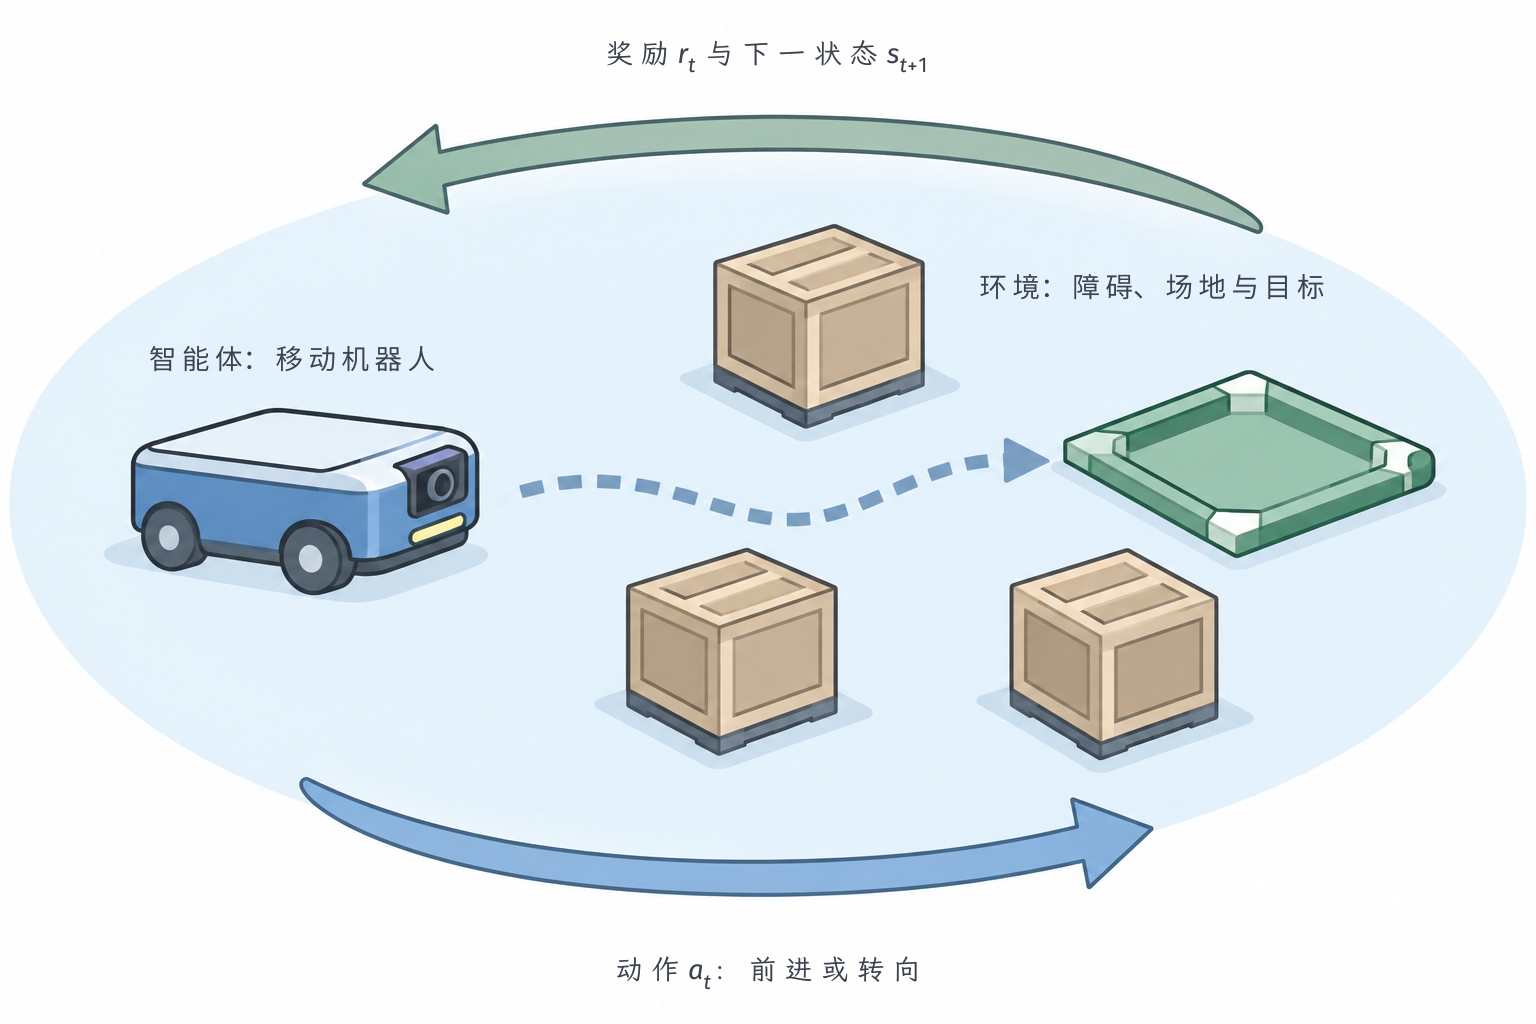
\includegraphics[width=157.400mm]{figures/10-reinforcement-learning/01-problems-and-solving/generated/rl-overview-embodied-loop/figure.png}
  \caption{完全可观测教学设定中的具身交互。移动机器人能够取得当前状态，据此选择动作；环境执行动作后改变场景，并返回奖励和下一状态。一般任务中机器人取得的是观测，观测未必揭示完整状态。插图只表达交互关系，不表示精确动力学、传感器结构或实验结果。}
  \label{fig:rl-overview-embodied-setting}
\end{figure*}

% Outline: 1.1
\Needspace{35mm}
\section{强化学习的基本设定}
\label{sec:rl-overview-setting}

% Outline: 1.1.1
\subsection{智能体与环境的交互}
\label{sec:rl-overview-interaction}

在仓储任务中，机器人可以提交前进、转向或停止等命令，却不能直接指定命令执行后的精确位置。地面摩擦、货箱位置和执行误差也会影响实际运动。我们把选择命令的主体称为\term{智能体}（agent），把命令给定后产生运动和反馈的过程称为\term{环境}（environment）。这种划分明确了学习算法能够改变的是命令选择规则，而不是任意改变物理后果。到达停靠区可以得到正奖励，碰撞或耗时可以产生代价；这些评分怎样共同评价任务，还需要另行规定。

为预测命令执行后的变化，需先规定用哪些变量描述当前环境。状态（state）是用于预测后续变化的环境描述，记为$s_t$；机器人的位置、朝向和障碍物位置可以共同组成一个状态。\term{状态空间}（state space）$S$收集任务中所有可能的状态，也就是这些变量在任务内允许出现的组合。动作$a_t$表示一次具体命令，\term{动作空间}（action space）$\mathsf A$则收集所有命令形式；这里的“动作”与前卷的“行动”指同一对象。命令可能只在某些状态下可执行，状态$s$下允许的命令组成$\mathsf A(s)\subseteq\mathsf A$。

环境状态与智能体实际取得的观测未必相同。观测（observation）是传感器或交互接口给出的测量结果，记为$o_t$：机器人的位置可以属于状态，相机拍到的局部图像则是观测。一张图像可能遮住了影响运动的障碍，因而不足以预测下一步。下面先假设智能体能够直接读出完整状态，即$o_t=s_t$，再将一次命令及其后果组成交互记录。

\begin{definition}[智能体、环境与一步经验]
  \label{def:rl-overview-interface}
  设$S$为状态集合，$\mathsf A$为动作集合，$\mathsf A(s)\subseteq\mathsf A$为状态$s$下非空的允许动作集合。离散时刻$t=0,1,\ldots$的状态为$s_t\in S$，所选动作为$a_t\in\mathsf A(s_t)$。智能体是依据可得观测和历史选择动作的主体，环境是在动作给定后产生后继状态与反馈的过程。在完全可观测（fully observable）设定下，观测$o_t=s_t$。执行$a_t$后取得奖励$r_t\in\mathbb R$和后继状态$s_{t+1}$，四元组
  \[
    (s_t,a_t,r_t,s_{t+1})
  \]
  称为一步经验，也称一步交互记录。$r_t$按动作发生的时刻编号，表示执行$a_t$之后得到的反馈。
\end{definition}

决策历史记为$I_t$，由行动前已取得的观测、过去动作及可见奖励组成。智能体只能利用当时已经取得的这些记录选择动作，不能读取尚未发生的奖励。本章先取$o_t=s_t$，不完整观测下怎样利用$I_t$由第~\ref{chap:rl-information}章处理。状态、观测与决策依据的区分沿用前卷的共同学习框架。

我们用网格位置作为状态，把上述接口缩小到一个可以手算的任务。网格宽$4$、高$3$，坐标为$x=1,\ldots,4$、$y=1,\ldots,3$；起点为$(1,1)$，终点为$(4,3)$，障碍$(2,2)$不可进入。到达终点的那一步得$1$，其余非终止步得$-0.04$。这些数值是教学假设，不是实验测量。方向命令可能因滑移而执行偏离，因此下面三条记录可以依次发生：
\[
\begin{aligned}
 &((1,1),\text{右},-0.04,(2,1)),\\
 &((2,1),\text{右},-0.04,(2,1)),\\
 &((2,1),\text{右},-0.04,(3,1)).
\end{aligned}
\]
第二条记录中，命令仍是向右，位置却没有改变。这可以由滑向障碍或边界造成，不能据此把动作改记为“停留”。经验同时保留命令和结果，才能区分选择规则与执行误差。

取得交互记录以后，学习规则才能据此构造训练目标并调整策略。图~\ref{fig:rl-overview-loop}用实线表示每步执行，用虚线表示记录收集和参数更新：采集器可以每步记录，参数更新却可以每积累一批记录才执行一次。部署时也可以固定参数，只保留执行闭环。因此，交互次数与梯度更新次数需要分别计算。

参与拟合的有限记录组称为训练样本，记为$D=(Z_1,\ldots,Z_n)$。每条$Z_i$可以是一条一步交互记录，也可以是一段完整轨迹；$Z_i$具体表示什么，必须随采集协议一并说明。这里特意保留记录的先后顺序和重复出现：机器人沿一条轨迹连续行动，相邻记录本就相互影响，同一种意外也可能多次发生，因此不能默认这些记录像独立抽签那样互不相关。除训练样本外，还可以按记录的用途划分另外两组：用于在候选规则之间作比较、帮助选择的称为验证样本$D_{\mathrm{va}}$；选择完成后，再用一组没有参与选择的记录独立检验最终规则，称为测试样本$D_{\mathrm{te}}$。训练、验证与测试描述的是同一批可能格式相同的记录被怎样使用，而不是记录来自真实机器人还是仿真程序。

怎样使用训练记录，还取决于允许在哪些行为规则中作选择。考虑一个最简单的情形：暂时只允许在两份事先写好的导航规则之间选择，每份规则在每个状态下都给出合法命令。这两份规则就划定了候选范围；而根据采集到的记录比较二者、并从中选出一份的那套计算过程，则属于选择程序。候选范围回答“可以选什么”，选择程序回答“凭记录怎样选”，两者即使都已确定，也还没有指出某次训练最终会选中哪一份——那要看具体记录与程序中的随机因素。

一般的策略学习也保留同样的层次，只是把候选规则记为策略，把候选范围记为候选策略类$\Pi$。学习规则需要完整规定四件事：允许哪些候选、怎样由训练样本构造比较用的目标、参数怎样初始化和逐步更新、以及何时停止并读出策略。先固定这些规则、训练配置和计算预算，单次拟合所得策略可以记为$\pi_D=A(D,U)$：$A$是从训练样本及随机源到候选策略的学习映射，$U$汇集初始化、抽样等算法随机性。这里$D$是程序使用的有限交互记录组，$A$规定怎样使用这些记录，$\pi_D$是这一次拟合得到的候选策略；某一步实际选出的动作又是执行该策略的结果。训练样本、学习映射、拟合所得策略和执行动作由此分属四个不同层次。

若还要利用验证样本选择超参数或检查点，固定训练样本与拟合随机数就不足以确定最终部署策略。为写清这层依赖，将参与拟合的样本也记为$D_{\mathrm{tr}}=D$，用$\eta\in\Lambda$表示允许选择的训练配置，$A_\eta$表示固定配置后的拟合映射；这些映射给出的候选策略都属于共同的$\Pi$。把拟合与选择使用的随机源合记为$U=(U_{\mathrm{fit}},U_{\mathrm{sel}})$，整个程序可写成
\[
 \widehat\eta=\operatorname{Select}(D_{\mathrm{tr}},D_{\mathrm{va}},U),
 \qquad
 \pi_{\mathrm{final}}
 =A_{\widehat\eta}(D_{\mathrm{tr}},U_{\mathrm{fit}})
 =A_{\mathrm{final}}(D_{\mathrm{tr}},D_{\mathrm{va}},U).
\]
选择规则还须规定怎样比较验证结果和处理并列；若验证结果决定何时停止，停止程序也属于$A_{\mathrm{final}}$。要进一步讨论最终策略的随机分布，还要求选择规则以及$(\eta,D_{\mathrm{tr}},U_{\mathrm{fit}})\mapsto A_\eta(D_{\mathrm{tr}},U_{\mathrm{fit}})$联合可测，从而上述复合程序仍是可测映射。例如，两份候选导航策略在同一训练样本上已经拟合完，另一次验证可能改变它们的回报排序，进而改变部署时选中的策略。执行阶段固定的是全部拟合与选择完成后的$\pi_{\mathrm{final}}$，再依据当前观测或决策历史选择动作，而不能把验证样本对最终结果的影响隐藏在一次固定配置的拟合映射里。

改变规则后，机器人可能进入此前很少经过的区域，新采集的训练记录随之改变分布。常见的监督学习基准分析把训练样本的生成规律视为固定；强化学习则必须额外处理“策略改变后，后续训练样本的分布也跟着改变”这层闭环关系。需要说明的是，监督学习的技术手段仍然可以用于这样的闭环，这里区分的是两类问题设定，而不是把两类技术割裂开来\scite{sutton2018}。

\begin{figure}[htbp]
  \centering
  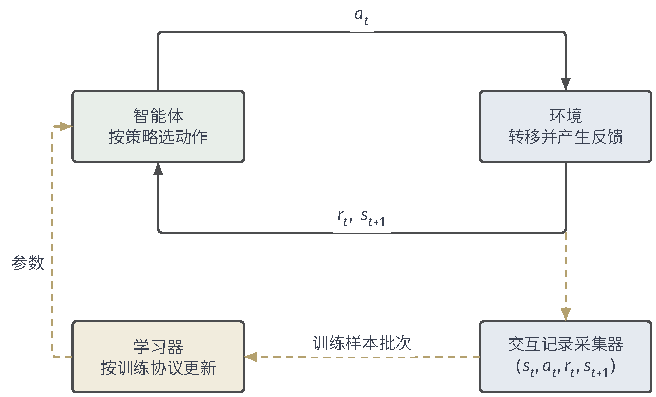
\includegraphics[width=111.100mm]{figures/10-reinforcement-learning/01-problems-and-solving/tikz/rl-overview-loop.pdf}
  \caption{交互与学习的接口。实线是每步执行的动作和反馈，虚线是经验收集及按训练协议发生的参数更新。部署时可移除虚线部分而保留执行闭环。}
  \label{fig:rl-overview-loop}
\end{figure}

% Outline: 1.1.2
\subsection{马尔可夫决策过程}
\label{sec:rl-overview-mdp}

前面三条经验只告诉我们已经发生了什么。它们无法回答一个对决策更关键的问题：如果在同一个位置改选其他动作，结果会怎样？已发生的记录里根本没有这种尝试，因此单凭记录本身无法比较没有执行过的命令。要在行动之前就算出每个选择的可能后果，我们需要一个环境模型：对每个状态和动作，给出它可能导致的下一状态、奖励，以及各种结果出现的概率。

在写出这份模型之前，先引入一个能大幅简化计算的假设。若给定当前状态与动作后，后果的条件分布不再随更早的历史改变，那么预测这一步时就无需翻出过去的观测、动作和奖励，只需知道现在处在哪个状态、准备执行什么命令。这一条件称为马尔可夫性（Markov property）。它不是在断言“真实世界没有历史”，而是在要求所选状态已经概括了过去观测、动作与奖励记录中预测下一步后果所需的部分；它的实际好处是让我们能够始终从当前状态开始向前计算，而不必逐次重放整段经历。

把这样的转移规律与可选动作结合，就得到\term{马尔可夫决策过程}（Markov decision process, MDP）。顾名思义，它是一个“做决策”的过程：描述智能体在哪些状态可以选哪些动作，以及每次选择之后按什么概率产生后果。它只负责给出决策所面对的环境规则，至于按什么规则做选择、用什么长期目标评价选择，仍需另行指定。在有限网格中，用$p(s',r\mid s,a)$表示给定$s,a$后下一状态为$s'$且奖励为$r$的联合概率，用$\mu_0$表示起始状态的分布。对同一状态动作下的所有奖励求和，就得到下一状态本身的概率；按各结果的概率对奖励加权，则得到这一步的平均评分。

为与前卷的一般记号衔接，动态环境记为$\mathcal E=(S,\Sigma_S,\mathsf A,\Sigma_A,\mu_0,T)$。其中$\Sigma_S,\Sigma_A$分别规定状态与动作中哪些子集算作可讨论概率的事件，是连续空间下严格表述所需要的对象；$T(s,a,B)$表示在$s$执行$a$后，下一状态落入事件$B$的概率。有限空间中可简写为$T(s'\mid s,a)=T(s,a,\{s'\})$；连续空间中则对应$T(\mathrm ds'\mid s,a)$这样的概率核写法。本卷额外使用联合核$p$，是为了把奖励与下一状态绑定在一起、保留二者的相关性；把$p$对奖励求和所得的状态边缘，恰好就是$T$。阅读时注意区分四个对象：环境$\mathcal E$是后果规律，策略$\pi$是选择规则，一次观测$o_t$是单个测量值，一批训练样本$D$是有限条记录，它们处在不同层次。

除了马尔可夫性，还要说明后果规律是否随时刻改变。下面先假设在同一状态执行同一动作时，下一状态与奖励的分布不看钟表上的绝对时刻都相同，这称为时间齐次（time homogeneous）。这两个条件回答的是两个独立的问题：马尔可夫性限制的是“给定现在后，是否还依赖更早的过去”，时间齐次限制的是“同一规律是否随时间推移而变化”。一个过程可以只满足其中之一，使用时不要混为一谈。若转移或奖励规律确实随时刻变化，可以把核改写为$p_t$，再对每个时刻分别检查马尔可夫条件。

\begin{definition}[马尔可夫决策过程]
  \label{def:rl-overview-mdp}
  设$(S,\Sigma_S)$、$(\mathsf A,\Sigma_A)$分别为状态和动作的可测空间，$\mathsf A(s)$是每个状态下非空的可行动作集合，$\mu_0$是$S$上的初始分布。时间齐次的联合转移奖励核$p(\mathrm ds',\mathrm dr\mid s,a)$从合法状态动作对生成$S\times\mathbb R$中的后继状态和奖励；固定$(s,a)$后它是概率测度，固定后果事件后它关于$(s,a)$可测。该结构配以时域和评价目标，构成所讨论的马尔可夫决策过程。状态、动作与奖励有限或可数时，以$p(s',r\mid s,a)$记点质量，要求$p\geq0$、$\sum_{s',r}p(s',r\mid s,a)=1$。马尔可夫性表示：给定当前状态动作后，下一状态与奖励的条件律不再依赖更早历史；在正概率历史上写为
  \begin{equation}
    \mathbb P(s_{t+1}=s',r_t=r\mid s_0,a_0,r_0,\ldots,s_t,a_t)
    =p(s',r\mid s_t,a_t).
    \label{eq:rl-overview-markov}
  \end{equation}
  当状态与奖励取值有限或可数时，转移边缘可以通过对奖励求和得到。要把平均一步评分定义为有限实数，还须对每个合法$(s,a)$假设
  $\sum_{s',r}p(s',r\mid s,a)|r|<\infty$。在此条件下，
  \begin{equation}
  \begin{aligned}
    T(s'\mid s,a)&=\sum_r p(s',r\mid s,a),\\
    R(s,a)&=\sum_{s',r}p(s',r\mid s,a)r.
  \end{aligned}
  \label{eq:rl-overview-kernels}
  \end{equation}
  $T$是转移核，给出每种后继状态的概率；$R$是给定状态动作后的条件期望奖励。连续状态或奖励时把相应求和改为对联合核的积分，并保留绝对可积条件。
\end{definition}

将定义用于网格，我们就能补全尚未给出的概率。$S$包含除障碍外的$11$个格子，起点固定，故$\mu_0((1,1))=1$。动作名称是上、下、左、右；意图方向会越界或进入障碍的命令不在$\mathsf A(s)$内。合法命令以$0.8$概率沿意图方向移动，以各$0.1$概率向两侧垂直方向滑移。滑移若撞墙或遇到障碍，则留在原位。

终点记为$g=(4,3)$。到达终点后，任务本已结束，但后文有时希望把“到达之后”也统一写成一条仍在继续的无限序列，以便对所有时刻使用同一套求和公式。为此引入一个约定：到达后只保留虚拟动作“停留”，满足$T(g\mid g,\text{停留})=1$，且后续奖励恒为$0$。这种一旦进入就不再离开的状态称为吸收状态（absorbing state）。它纯粹是记账上的补全——终止后的记录既不增加也不减少任务收益，却让无限时域折扣目标可以直接沿用；后续讨论中我们将一直采用这一约定。

这项任务按实际后果计分，而不是按意图计分。从非终点状态出发，若$s'=g$就返回$1$，否则返回$-0.04$。在$(3,3)$选右时，有$0.8$概率到终点、$0.1$因上方边界留在原位、$0.1$滑到$(3,2)$。要在执行前评价这一步的平均评分，需按这些概率加权，得到
\[
  R((3,3),\text{右})=0.8\times1+0.2\times(-0.04)=0.792.
\]
其中$0.792$是重复执行时的期望，不是环境每次返回的奖励；一次实际反馈仍是$1$或$-0.04$。一次样本不能确定期望，期望也不能唯一确定全部奖励分布。联合核$p$保留了后继状态与奖励的对应关系，而$T,R$分别汇总其中的状态概率和平均评分。

上述模型把网格位置当作充分状态，其前提是：位置相同、动作相同时，更早的历史不会再改变后果分布。这一前提并不总成立。设想网格新增一扇门，而此前是否取到钥匙会改变门此刻能否通行；那么同样站在门前、坐标完全相同的两个时刻，向前走的后果可能一个是穿过门、另一个是被挡住。只记$(x,y)$对预测未来就不再充分。补救办法是把门的通行状态$b\in\{0,1\}$一并写入状态$s=(x,y,b)$；在其余机制固定的情况下，增广后的状态才可能恢复充分性。这个例子同时说明式~\eqref{eq:rl-overview-markov}约束的对象是状态表示：当历史确实影响未来时，应当把相关历史吸收进状态，而不是假装历史无关。反过来，若$b$根本无法被传感器观测到，扩充符号也不能让智能体凭空知道门是开是关——状态增广解决的是后果描述是否充分，不能保证门的通行状态能够由传感器观测辨认。

有了状态、动作和转移概率，MDP仍缺最后一块拼图：怎样把不同时刻陆续得到的奖励合成为一个可以最大化的总目标。最简单的做法是只累计接下来$H$步的结果，任务到时即结束；也可以让任务持续运行，此时若把未来每一步都等权相加，总和通常会发散而无法比较，于是引入折扣因子（discount factor）$\gamma$：$k$步之后才拿到的奖励先乘上$\gamma^k$，越远的未来在总目标中占的比重越小。本章网格默认采用$\gamma=0.9$的无限时域折扣目标，并会明确标出与之独立的有限时域算例。表~\ref{tab:rl-overview-horizons}汇总四种常见设定；其中平均奖励考察长期平均每步收益，随机最短路累计到随机到达终点时刻为止的收益。这两类只作为了解边界的入口，它们的收敛条件不能直接照搬折扣问题的结论。

读这张表时，$V_H$表示时刻$H$之后剩余收益的期望，$V_H=0$即任务在末端不再计入任何后续收益。平均奖励一行还涉及策略长期运行时会落在哪些状态：固定策略会在状态空间上诱导一条转移链，需要考察长期是否进入稳定的循环区域、所得每步平均是否仍依赖起点。以有限状态情形为例，闭合互通类内的状态彼此可达，进入后不会离开；暂态状态可以在进入这些长期运行区域之前经过，在有限链中几乎必然只被访问有限次。所有状态彼此可达时，链称为不可约。表中的单链条件要求每份平稳确定性策略各自只产生一个闭合互通类，但仍允许存在暂态状态；这些条件是在约束长期运行结构，并不等于已经证明了任意策略的平均奖励结论。

\begin{table*}[htbp]
  \centering\small
  \begin{tabularx}{\linewidth}{@{}>{\raggedright\arraybackslash}p{24mm}*{3}{>{\raggedright\arraybackslash}X}@{}}
    \toprule
    设定 & 终止与时间 & 比较的目标 & 需另行检查的条件\\
    \midrule
    有限时域 & $t=0,\ldots,H-1$，$V_H=0$表示末端无后续收益 & $H$步期望奖励总和，可另指定折扣 & 剩余时间影响决策；可并入状态\\
    折扣无限时域 & 可持续运行；终止后补吸收状态 & $\mathbb E\sum_{t\geq0}\gamma^t r_t$ & $0\leq\gamma<1$；有界奖励使总和有限\\
    平均奖励 & 通常持续运行，不因目标达成停止 & $\lim_{n\to\infty}n^{-1}\mathbb E\sum_{t=0}^{n-1}r_t$ & 极限需存在；须检查策略诱导的状态转移链。链不可约时状态相互可达；若称MDP为单链，通常要求每份平稳确定性策略诱导的链仅有一个闭合互通类，另可含暂态\\
    随机最短路 & 在随机时刻$\tau$到达终点 & $\mathbb E\sum_{t=0}^{\tau-1}r_t$，常用成本形式 & 需检查到达性、期望终止时间与不可终止策略的代价\\
    \bottomrule
  \end{tabularx}
  \caption{同一状态动作接口可搭配不同时间目标。随机最短路中的“最短”可以指累计成本，不限于几何距离；取$\gamma=1$不能自动把折扣定理变成其余三类定理。}
  \label{tab:rl-overview-horizons}
\end{table*}

\Needspace{10\baselineskip}
上述几类MDP的系统性处理可见Puterman的专著\scite{rl1-puterman1994-mdp}

% Outline: 1.1.3
\subsection{动作}
\label{sec:rl-overview-actions}

% Outline: 1.1.3.1
\subsubsection{动作空间与可行动作}
\label{sec:rl-overview-action-space}

网格已经规定了上、下、左、右四个方向命令，但真实任务的一次选择未必能用有限个名称穷尽。受控机械系统可能需要输出一个连续的力向量$\bm u\in\mathbb R^m$，其中$m$是控制分量数；推荐系统需要同时选择若干项目并排列次序；抓取命令则可能先选离散的抓取方式、再给连续的位置参数。之所以要比较这些动作形式，是因为它们直接决定两件事：决策规则最终要输出什么类型的对象，以及在执行前应当用什么方式检查一条命令在当前状态下是否合法。

合法性首先由当前状态下的允许集合$\mathsf A(s)$决定。若规则用概率分布选择命令，记为$\pi(\cdot\mid s)$，就必须把全部概率放在这个集合内。这个记号只表示在状态$s$如何选动作，其完整类型将在策略一节定义。

\begin{definition}[合法动作与策略支持]
  \label{def:rl-overview-admissible}
  给定状态空间$S$、动作可测空间$(\mathsf A,\Sigma_A)$以及非空可测集合$\mathsf A(s)\in\Sigma_A$。从$S$到$\mathsf A$的概率核$\pi(\cdot\mid s)$是合法决策规则，当且仅当对每个$s\in S$有
  \[
    \pi(\mathsf A(s)\mid s)=1.
  \]
  对离散动作，这等价于$a\notin\mathsf A(s)$时$\pi(a\mid s)=0$，且合法动作的概率和为$1$。确定性规则必须输出$\mathsf A(s)$中的一个元素。
\end{definition}

在图~\ref{fig:rl-overview-grid-actions}中，$(1,1)$允许上和右；$(3,2)$允许上、下和右，但左边是障碍。这里排除的是\emph{意图方向}非法的命令，不是排除随机执行误差。另一种常见网格建模允许四个方向始终可选，把主动撞墙也规定为原地不动；那会增加可选行为，改变策略空间。本书贯穿网格采用前一种定义，只有随机滑移撞墙才留在原位。

\begin{figure}[htbp]
  \centering
  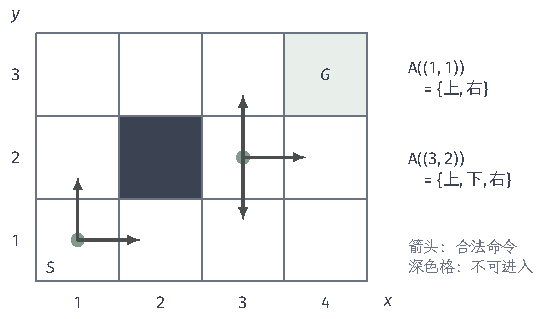
\includegraphics[width=92.019mm]{figures/10-reinforcement-learning/01-problems-and-solving/tikz/rl-overview-grid-actions.pdf}
  \caption{基准网格与两个位置的合法命令。实心方格是障碍，$S$和$G$分别表示起点与终点；箭头表示可选择的意图方向，不表示随机滑移的全部后果。}
  \label{fig:rl-overview-grid-actions}
\end{figure}

表~\ref{tab:rl-overview-action-types}按一次命令的数学形式列出输出与约束。这里的分类不涉及命令持续多久：一个持续若干步的技能仍可用离散编号或连续参数选择，只是决策时间尺度不同。这一变化由下一小节处理。

命令能够执行，也不等于执行它满足安全要求。执行器只能提供有限大小的力，是动作接口的限制；某个力在硬件上可用，却可能因碰撞风险而被禁用，则是根据行为要求进一步限制动作。两种限制可以同时进入允许集合，但安全条件怎样建立、能保证什么，需由第~\ref{chap:rl-trustworthy}章另行分析。

\begin{table}[htbp]
  \centering\small
  \begin{tabularx}{\linewidth}{@{}>{\raggedright\arraybackslash}p{19mm}*{2}{>{\raggedright\arraybackslash}X}@{}}
    \toprule
    数学形式 & 策略输出对象 & 约束接口的例子\\
    \midrule
    离散 & 一个动作编号或概率向量 & 方向掩码标出可用命令；仅对合法方向归一化\\
    连续 & 向量$\bm u$或其分布 & 力的上下界、联动约束\\
    组合 & 子集、排列或多项联合选择 & 推荐列表长度、项目去重、容量限制\\
    参数化 & 类型$c$及参数$\bm u_c$ & 不同类型有各自维度和参数范围\\
    \bottomrule
  \end{tabularx}
  \caption{动作的分类对象是一次命令的数学形式。执行器噪声属于转移机制，不会把离散命令自动变成连续动作。}
  \label{tab:rl-overview-action-types}
\end{table}

% Outline: 1.1.3.2
\subsubsection{动作后果与时间尺度}
\label{sec:rl-overview-time-scale}

在起点提交同一个向右命令，改变执行机制就会改变后果。表~\ref{tab:rl-overview-transition}固定$s=(1,1)$和命令，只对照确定移动与基准滑移。两者即时奖励都为$-0.04$，但确定移动总到$(2,1)$，随机移动还可能进入左侧竖向通道或留在起点。只看这一步的评分，就看不到后续可达区域的变化。确定移动仅是本表的对照条件，其余网格计算仍保留滑移。

\begin{table}[htbp]
  \centering\small
  \begin{tabular}{@{}lccc@{}}
    \toprule
    向右的后继状态 & 确定移动概率 & 基准概率 & 奖励\\
    \midrule
    $(2,1)$ & $1$ & $0.8$ & $-0.04$\\
    $(1,2)$ & $0$ & $0.1$ & $-0.04$\\
    $(1,1)$ & $0$ & $0.1$ & $-0.04$\\
    \bottomrule
  \end{tabular}
  \caption{同一向右命令在两种转移机制下的结果。基准的向下滑移越界，因此留在原位；零概率行仅用于对齐比较。}
  \label{tab:rl-overview-transition}
\end{table}

即使不改变机制，不同动作也可能具有相同即时奖励。在$(3,2)$选择上或下，当步都不可能到达终点，所以期望奖励同为$-0.04$。向上大概率到$(3,3)$，下一步即可尝试进入目标；向下大概率回到$(3,1)$，还需多次行动。一步评分无法表现这项差别。这里尚不声称某个动作必然最优，因为后续策略及随机转移也影响累计结果；它说明了为何需要一个跨越多步的评价对象。

动作的多步后果还要和奖励的记录时刻区分开。图~\ref{fig:rl-overview-timeline}上行沿一条可能发生的轨迹标出每次命令与反馈：执行$a_t$后得到$r_t$，而数步之后到达终点的那$1$分奖励只记录在真正到达的那一步。这就带来一个学习时无法回避的问题：当奖励很晚才出现时，应当如何用这个晚到的结果去评价早先作出的那些选择？例如终点奖励应归功于几步前那次关键转向，而不应平均分给沿途所有无关动作。这种判断哪些早先行动应对后来的收益或失败承担作用的工作，称为信用分配（credit assignment）。请注意，它改变的只是评价时如何引用历史，并不改变奖励实际发生的时间顺序——终点奖励依然发生在到达的那一刻。

\begin{figure*}[htbp]
  \centering
  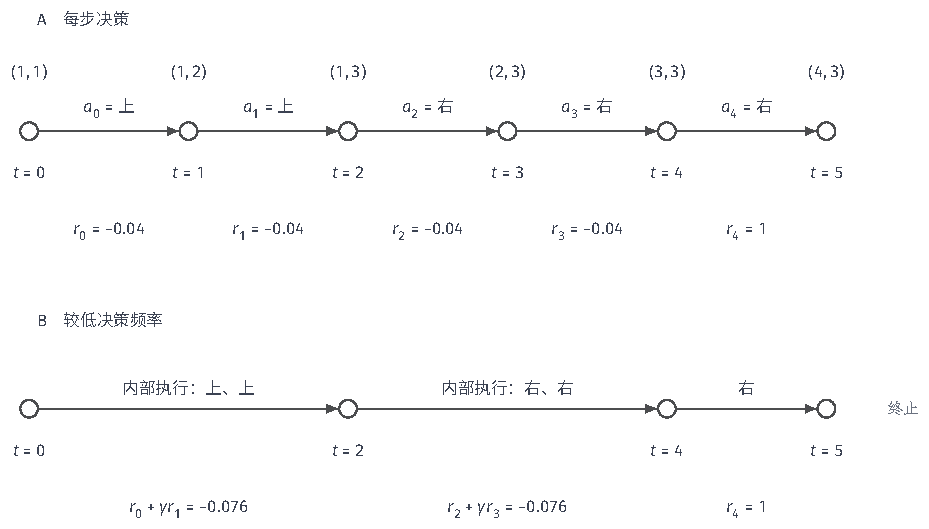
\includegraphics[width=157.371mm]{figures/10-reinforcement-learning/01-problems-and-solving/tikz/rl-overview-timeline.pdf}
  \caption{同一条五步到达轨迹的时间标记。上行每步决策，最后一个动作返回$r_4=1$；下行只在$t=0,2,4$重新决策。下行跨两步的箭头表示持有或执行内部命令的区间，不能仍用上行的一步核和单步奖励表示。}
  \label{fig:rl-overview-timeline}
\end{figure*}

图的下行改为每两步才重新决策一次。这一改变不只是少记录几个时刻：新接口下的一次动作跨过了两次原始转移，因此必须重新描述“两步之后”的状态分布，并把这期间累计的评分一并计入，不能继续套用原来的单步核和单步奖励。具体地，若一条命令持续$k$个原始步，在原始折扣$\gamma$下，区间内拿到的收益为$\sum_{j=0}^{k-1}\gamma^j r_{t+j}$；而从下一次决策时刻$t+k$才开始计算的后续累计收益，在折算回当前时刻$t$时还要整体再乘$\gamma^k$，因为它的第一项已经晚了$k$个原始步。例如两个非终止步的贡献是$-0.04+0.9(-0.04)=-0.076$，不能仍记成单个$-0.04$。若命令持续的步数本身是随机的，这段持续时间也必须作为动作后果的一部分纳入描述。

连续时间控制进一步以物理时间而非固定步号描述运动，用微分动力学或跳变机制表示变化，奖励常是单位时间的收益率。离散化时，状态变化和区间收益必须一起调整，不能只改变决策频率。本章保留这些接口区别，不把其目标混入固定步长MDP；跨步递归将在第~\ref{chap:rl-learning}章的时间抽象中展开。

% Outline: 1.1.4
\Needspace{7\baselineskip}
\subsection{策略}
\label{sec:rl-overview-policies}

% Outline: 1.1.4.1
\subsubsection{策略及其类型}
\label{sec:rl-overview-policy-types}

若网格移动没有任何误差，那么从起点依次执行“上、上、右、右、右”就能沿上路准确到达终点，此时一条事先排好的动作序列已经足够。但基准网格存在滑移：同一条命令可能把机器人带偏，一旦偏离，预先写好的余下命令就可能与当前实际位置不再匹配。这说明决策规则必须能够在行动过程中根据当前所在位置重新选择，而不是一次性写死整个动作序列。\term{策略}（policy）就是这样一条根据当前观测或决策历史选择行动的规则。此前记号$\pi(\cdot\mid s)$描述的正是它在状态$s$下给出的动作分布；某一步实际选出的$a_t$只是这条规则的一次抽样结果。

策略可以沿两个相互独立的维度变化。一个维度是规则是否随时间改变：在同一状态始终使用相同动作分布的，称为平稳策略（stationary policy）；允许这份分布随时刻变化的，称为非平稳策略（nonstationary policy）。另一个维度是给定状态后如何取值：每次只指定一个确定动作的，称为确定性策略（deterministic policy）；按一份概率分布抽样动作的，称为随机策略（stochastic policy）。这两个维度必须分别记录——是否随机抽样，与是否依赖时间并无关系，不能从一个性质推断另一个。

在有限动作情形下，固定一个状态$s$，策略给出的就是一份各动作概率组成的向量；换一个状态，这份向量可以完全不同。要把“给定状态后产生一份动作分布”的规则写到一般空间上，就使用下面的概率核记号。确定性规则把全部概率集中在同一个动作上，这种点质量分布称为Dirac分布；它仍然是一份合法的概率分布，只是取某个动作的概率为$1$，并没有改变策略作为“状态到分布的映射”这一对象类型。

\begingroup
\binoppenalty=10000
\relpenalty=10000
\begin{definition}[马尔可夫策略]
  \label{def:rl-overview-policy}
  给定状态可测空间$(S,\Sigma_S)$、动作可测空间$(\mathsf A,\Sigma_A)$及非空可测动作集合$\mathsf A(s)$。马尔可夫策略序列为$\pi=(\pi_t)_{t\geq0}$，其中每个$\pi_t(\mathrm da\mid s)$是从$S$到$\mathsf A$的概率核，并对每个$s$满足$\pi_t(\mathsf A(s)\mid s)=1$。动作有限或可数时，以$\pi_t(a\mid s)$记点质量；当$\mathbb P_\pi(s_t=s)>0$时，它等于$\mathbb P_\pi(a_t=a\mid s_t=s)$。这里的马尔可夫策略在给定$t$后只使用当前状态，不再依赖此前历史。若规则不显式依赖$t$，记为$\pi(\mathrm da\mid s)$，称为\term{平稳策略}；否则称为非平稳策略。若每个状态只输出一个合法动作$f_t(s)$，则为确定性策略；一般动作空间上对应以$f_t(s)$为原子的Dirac核，有限或可数动作下其点质量可写为$\pi_t(a\mid s)=\mathbf 1\{a=f_t(s)\}$。
\end{definition}
\endgroup

更一般的策略可以依赖全部可用历史，写成$\pi_t(\mathrm da\mid I_t)$；有限或可数动作下仍用$\pi_t(a\mid I_t)$表示点质量。本章完全可观测的主线使用上述马尔可夫策略，但不据此宣称在任何约束或观测与历史访问条件下当前状态都足够。表~\ref{tab:rl-overview-policy-types}展示抽样与时间依赖的四种组合：固定概率抽样可以是平稳的，每次确定地选择动作也可以随剩余时间改变。

\begin{table}[htbp]
  \centering\small
  \begin{tabularx}{\linewidth}{@{}>{\raggedright\arraybackslash}p{21mm}*{2}{>{\raggedright\arraybackslash}X}@{}}
    \toprule
    & 确定性 & 随机性\\
    \midrule
    平稳 & 在起点总选上 & 在起点始终以$0.7$选上、$0.3$选右\\
    非平稳 & 根据剩余步数改选近路或远路 & 剩余时间多时以$0.7$选上，少时改为$0.2$\\
    \bottomrule
  \end{tabularx}
  \caption{两种互不等同的策略属性。表中的概率是教学规则，不是估计结果；各状态仍须满足各自的动作合法性。}
  \label{tab:rl-overview-policy-types}
\end{table}

有限时域为何可能需要时间？考虑一个从导航任务简化出的独立岔路例：取消滑移和步成本，近路只需一步即以$0.4$概率得到终点奖励$1$，否则以奖励$0$终止；绕路需要两步，必得$1$。在不折扣且到时终止的规则下，只剩一步时近路期望为$0.4$、绕路为$0$；还剩两步时两者为$0.4$和$1$。同一岔路的选择随剩余时间改变。把剩余时间加入状态可以重新用平稳形式书写，但这相对于增广状态而言，并没有消除实际的时间依赖。

图~\ref{fig:rl-overview-policy-randomness}在基准起点画出两份动作概率。一份以$1$的概率选择上，另一份以$0.7$选上、$0.3$选右。即使采用第一份规则，下一状态仍以$0.8$概率为$(1,2)$、$0.1$为$(2,1)$、$0.1$留在起点。策略确定只能消除选动作时的随机性，不能消除转移随机性。状态与动作均有限的无限时域折扣MDP何时存在最优确定性平稳策略，是第~\ref{chap:rl-planning}章要证明的结论，不是策略一词本身的含义。

\begin{figure}[htbp]
  \centering
  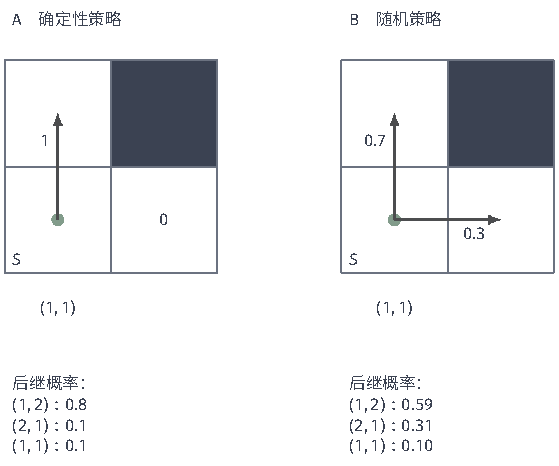
\includegraphics[width=94.580mm]{figures/10-reinforcement-learning/01-problems-and-solving/tikz/rl-overview-policy-randomness.pdf}
  \caption{同一网格起点的两种动作分布。左边确定性策略仍有随机后继；右边额外引入动作选择的随机性。图只显示起点附近，未画出的位置沿用基准网格。}
  \label{fig:rl-overview-policy-randomness}
\end{figure}

% Outline: 1.1.4.2
\subsubsection{策略诱导的轨迹与样本}
\label{sec:rl-overview-occupancy}

起点选上与选右，会把机器人带向不同区域。要计算某份策略会产生哪些训练记录，我们先求一段记录出现的概率。把包含$H$步的有限轨迹记为$\tau_H=(s_0,a_0,r_0,\ldots,s_{H-1},a_{H-1},r_{H-1},s_H)$。下面先沿有限或可数状态、动作和奖励的点质量写法计算；一般空间上的轨迹分布须逐步应用策略核与环境核，对事件作相应积分，不能把连续变量的单点概率当作密度。概率链式法则按发生顺序展开联合概率；马尔可夫性把每步环境条件缩减为当前状态动作，马尔可夫策略则给出该时刻的动作概率。因此，
\begin{equation}
  \mathbb P_\pi(\tau_H)
  =\mu_0(s_0)\prod_{t=0}^{H-1}
    \pi_t(a_t\mid s_t)\,p(s_{t+1},r_t\mid s_t,a_t).
  \label{eq:rl-overview-trajectory}
\end{equation}
初始位置来自$\mu_0$，动作来自$\pi_t$，反馈来自环境核$p$。这里使用的概率链式分解按发生顺序逐层条件化，不要求各时刻独立；同一联合律下再按中间变量取条件期望，便可把多步平均分层计算。链式分解和条件期望的迭代性质可参考\BookChapterRef{chap:random-variables}{卷2《数学准备：概率、因果与决策》的“随机变量与概率基础”章}。若只关心状态动作轨迹，对奖励求和后便得到含$T(s_{t+1}\mid s_t,a_t)$的乘积；不能直接把$p$替换为“奖励恒等于$R(s,a)$”。若策略依赖历史，链式分解依然成立，但动作项须改写为$\pi_t(a_t\mid I_t)$。

将这个轨迹分布记为$P_{\mathcal E}^{\pi}$；该简记还固定了奖励联合规律、观测机制与时域。本章状态完全可见，观测核为$K_o(s,\cdot)=\delta_s$。由于$o_t=s_t$，轨迹中可省写观测。部分可观测时，理论轨迹还须纳入观测机制生成的$o_0,\ldots,o_H$；实际训练记录则只能保留已经采集的字段，不能直接读出隐藏状态。

为区分这两个层次，先按理论轨迹分布生成一条轨迹，再用可测记录映射$b$保留实际可见的字段。不同的隐藏轨迹可能留下同一份可见记录；要计算某类记录出现的概率，就要把所有能生成这类记录的轨迹作为同一事件来计概率。可见记录分布记为$P_{\mathrm{rec}}^{\pi}=b_{\#}P_{\mathcal E}^{\pi}$，其中推前记号的事件读法是：对可见记录空间中的任意可测事件$C$，
\[
 P_{\mathrm{rec}}^{\pi}(C)
 =P_{\mathcal E}^{\pi}\bigl(\{\tau:b(\tau)\in C\}\bigr).
\]
右侧先在理论轨迹中找出经$b$映入$C$的全部情形，再按原轨迹分布计算这个事件的概率。本章保留可见状态时，不需要删去这些状态字段；改变观测或记录机制时，则须恢复相应依赖，不能把理论轨迹的全部状态直接当成训练记录。

沿用第~\ref{sec:rl-overview-interaction}节的三步记录，若在$(1,1)$与$(2,1)$都必选右，其概率为$0.8\times0.2\times0.8=0.128$。中间的$0.2$是两种被阻挡的滑移概率之和。只把起点改为以$0.3$概率选右，保持后两次必选右，同一记录的概率就变为$0.0384$。环境核没有改变，训练记录的分布却随策略改变了。

完整轨迹的可能种类很多，而比较不同策略会产生什么样的训练记录时，往往不必逐一罗列整条轨迹，只需知道在各个时刻、机器人有多大概率处在某些状态并采取某些动作。为此先看固定某一时刻$t$的分布，称为逐时分布（time-marginal distribution），它记录该时刻遇到各状态、各动作的概率。若还想把无限多个时刻汇总成一份分布，就必须约定不同时刻各占多大权重。由于折扣目标认为越早的后果越重要，我们自然用$\gamma^t$对逐时分布加权，再乘上$1-\gamma$使全部权重之和恰好为$1$。汇总所得的\term{折扣占用度量}（discounted occupancy measure）就是一份状态动作分布，回答这样一个问题：若按策略运行、并按这些折扣时间权重随机抽取一个时刻，那个时刻会看到什么状态、正在做什么动作。下面的$q_t^\pi(s,a)$、$d^\pi(s,a)$及求和仍采用有限或可数空间的点质量写法；一般空间上应把它们定义为状态动作集合上的测度，并将求和改为积分。

\begin{definition}[逐时分布与折扣占用度量]
  \label{def:rl-overview-occupancy}
  给定有限或可数状态动作空间上的时间齐次MDP、初始分布$\mu_0$及合法马尔可夫策略序列$\pi$。以$\mathbb P_\pi$表示它们诱导的轨迹律，逐时状态分布为$q_t^\pi(s)=\mathbb P_\pi(s_t=s)$，状态动作分布为$q_t^\pi(s,a)=q_t^\pi(s)\pi_t(a\mid s)$。对$0\leq\gamma<1$，归一化的折扣占用度量为
  \begin{equation}
    d^\pi(s,a)=(1-\gamma)\sum_{t=0}^{\infty}
      \gamma^t q_t^\pi(s,a),\qquad
    d^\pi(s)=\sum_a d^\pi(s,a).
    \label{eq:rl-overview-occupancy}
  \end{equation}
\end{definition}

我们可以把这种加权写成一次抽样：取独立于轨迹的时刻$T$，满足$\mathbb P(T=t)=(1-\gamma)\gamma^t$，则$\mathbb P_\pi(s_T=s,a_T=a)=d^\pi(s,a)$。它不是一条轨迹中“至少到访一次”的概率，反复到访与晚到访都会影响加权结果。要核对$d^\pi$确实归一化，可利用各项非负交换求和次序，再用每一时刻的概率质量为$1$：
\[
  \sum_{s,a}d^\pi(s,a)
  =(1-\gamma)\sum_{t=0}^{\infty}\gamma^t
    \underbrace{\sum_{s,a}q_t^\pi(s,a)}_{1}=1.
\]
终止后必须保留吸收状态及其虚拟动作，以上质量才仍然为$1$；若把终止后的时刻全部删除，得到的是非终止占用，其总质量一般小于$1$。吸收状态的占用高也不表示在那里继续取得奖励，因为其奖励为零。

另取只有起点$x$与吸收终点$g$的两状态教学任务，从$x$一步必到$g$，以后一直停留。取$\gamma=0.9$，只有时刻0位于$x$，因而$d(x)=0.1$、$d(g)=0.1\sum_{t\geq1}0.9^t=0.9$。两处都必定到访，至少到访一次的概率却都是1。占用描述按折扣权重抽到的时刻在哪里，不是有没有到访过；若进入$g$时奖励1、此后奖励0，回报为1，也不能把终点占用0.9当作回报。

平稳策略还满足$d^\pi(s,a)=d^\pi(s)\pi(a\mid s)$，因为每个时刻在$s$的动作分布相同。非平稳策略的占用仍由式~\eqref{eq:rl-overview-occupancy}定义，但不能把随时间变化的$\pi_t$直接提出求和号。这一区别在后续利用占用度量恢复平稳策略时会用到。

图~\ref{fig:rl-overview-occupancy}把加权分布用于比较两份完整的确定性策略。箭头给出每个非终点格的唯一意图方向，深浅及数字表示$d^\pi(s)$，不是价值。计算时先从$q_0=\mu_0$出发，对当前状态概率、动作概率和后继概率逐层加权，将分布传播到下一步：
\[
 q_{t+1}^\pi(s')=\sum_s q_t^\pi(s)
                    \sum_a\pi(a\mid s)T(s'\mid s,a)
\]
再按式~\eqref{eq:rl-overview-occupancy}累加各时刻分布。保留$400$个时刻时，总质量尾差为$0.9^{400}<5\times10^{-19}$。两幅图采用同一色标：上路策略在左侧通道的占用较大，下路策略则更多到访底边。

占用还可以联系到一项明确的记录计数协议。固定策略与初始分布，独立重复生成轨迹；每次按前述几何权重抽一个独立于轨迹的时刻，再保留该时刻的状态动作记录。若共保留$n$条这样的记录，区域$B\subseteq S$中的记录数，其期望为$n\sum_{s\in B}d^\pi(s)$。因此，在相同折扣时间权重和记录预算下，两份策略会提供不同的期望区域记录数；一份有限样本的实际计数仍有波动。这里$n$按保留的记录计数，生成这些记录消耗的真实环境交互步数须另行计算。

\begin{figure*}[htbp]
  \centering
  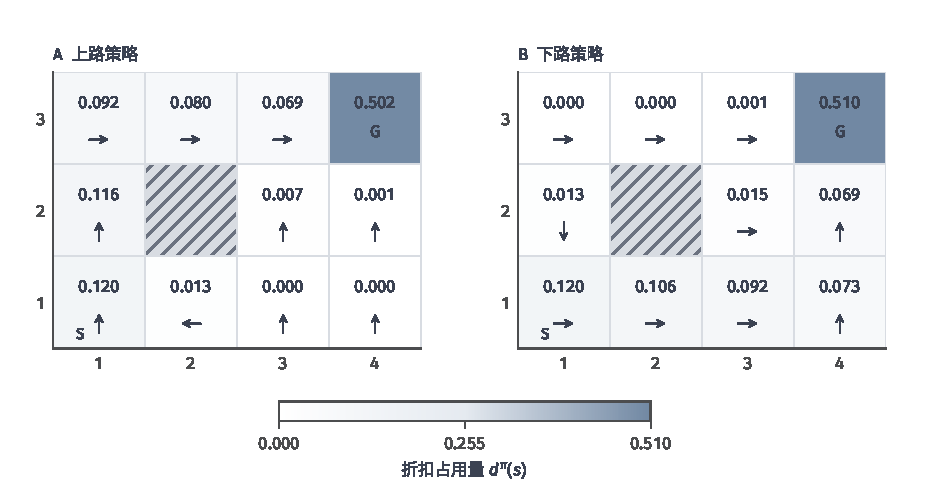
\includegraphics[width=157.400mm]{figures/10-reinforcement-learning/01-problems-and-solving/matplotlib/rl-overview-occupancy.pdf}
  \caption{基准随机网格中两份策略的归一化折扣状态占用，$\mu_0$集中于起点，$\gamma=0.9$。箭头是确定性策略，滑移仍为$0.8/0.1/0.1$；数字四舍五入至三位小数，障碍不是零概率的可用状态。}
  \label{fig:rl-overview-occupancy}
\end{figure*}

这种训练样本生成规律的差异，在“想用旧规则跑出来的经验去评价或改进一条新规则”时尤为关键，因此需要为两条规则分别命名。实际负责采集训练样本、决定日志如何产生的规则称为\termalias{rl-behavior-policy}{行为策略}（behavior policy），记为$\beta$；而我们真正想评价或改进、想知道其后果的规则称为\term{目标策略}（target policy），记为$\pi$。二者恰好相同时，称为同策略（on-policy）问题，即“用谁就评价谁”；二者不同时，称为离策略（off-policy）问题，即“用一份规则的记录去推断另一份规则”。还要注意这一划分与在线、离线的划分不同：同策略与离策略比较的是行为规则和目标规则是否为同一条，在线与离线说的则是训练过程中能否继续追加新的交互记录，两组概念互不蕴含。

用$\beta$的记录去推断$\pi$的后果，首先要检查这些记录是否覆盖了目标规则真正需要的状态和动作。如果行为分布对某个必要动作赋予的概率始终为零，那么已有样本再多，也无法靠重新加权凭空生成该动作的后果。这就是覆盖（coverage）问题：训练样本的生成规律必须为待推断的行为提供足够支持，关键不在于记录总数多，而在于关键的状态动作是否真有机会被采到。

训练样本的联合律还要由采样机制$\Gamma_{\mathrm{tr},n}$指定，不能只由单条记录分布推出。例如，从同一条长轨迹中截取相邻转移，与每次重置后独立采集完整回合，会产生不同的记录间依赖；采样机制要说明采取哪一种协议，以及每条$Z_i$保留什么。

在以固定$\beta$、按同一协议独立重复采集完整回合的基准设定中，若每条$Z_i$是一个回合的可见记录，就有$D\sim(P_{\mathrm{rec}}^\beta)^n$，右侧的幂表示$n$份回合记录的乘积分布。全部拟合与验证选择完成后，冻结最终策略$\pi$，用新的环境随机性独立运行$m$个测试回合。给定这份最终策略及固定的测试协议，便有$D_{\mathrm{te}}\sim(P_{\mathrm{rec}}^\pi)^m$；右侧是条件于所选策略后的乘积律。这里$m$是测试回合数。也可以先给定全部训练样本、验证样本和拟合与选择随机源，使最终策略固定，再说明测试回合的条件独立性；仅固定训练样本和拟合随机源，不足以排除验证选择造成的共同依赖。若只能使用旧日志，留出的评价记录仍由行为策略生成，必须通过离策略评价联系目标回报，不能假定它们已来自$\pi$。

在$(2,1)$，合法动作是左、右，两侧滑移都只会停留。若$\beta$在此永远选左，日志就没有从该格主动向右的样本，尽管$\pi$可能需要向右。另一种情况是$\beta$允许进入左侧通道，但某份有限日志恰好没到过那里。前者是行为分布本身不支持必要动作，后者可能只是有限抽样遗漏，二者不能混为同一结论。

跨位置推断可以借助函数逼近（function approximation），也就是让不同位置的预测共享参数；其可靠性仍需结构假设和相应的交互记录。网络能输出一个未尝试动作的预测，不等于该预测已被验证。占用的流守恒及由占用恢复策略将在第~\ref{chap:rl-planning}章展开，离策略覆盖的后果则由第~\ref{chap:rl-information}章进一步分析。

% Outline: 1.1.5
\subsection{奖励}
\label{sec:rl-overview-rewards}

% Outline: 1.1.5.1
\subsubsection{奖励与累计回报}
\label{sec:rl-overview-return}

策略决定怎样行动，奖励规则则决定怎样给行动后果计分。基准网格对每个非终止步收取$0.04$的代价、到达终点给$1$，这两条数值同时表达了两种偏好：希望到达目标，也希望不要拖延。但单步评分很快就不够用了：在远离终点的位置，绝大多数动作的即时奖励都是同一个$-0.04$，只比较这一个数字，根本无法区分一个动作是把机器人带向终点还是带向死路。因此评价一个动作时，必须把它之后陆续获得的奖励也一起算进来。\term{回报}（return）就是按约定的时间规则把一串奖励累计成的一个总分，用一个数概括整段行动的好坏。

沿用前面引入的折扣因子，折扣回报对$k$步之后的奖励乘权重$\gamma^k$。当$0<\gamma<1$时，越遥远的收益权重越小，这同时保证无限序列的总分通常仍是有限数；$\gamma=0$时则退化为只计当前一步。还需注意，对随机策略和随机转移而言，同一份策略可能产生许多条不同轨迹、对应许多个不同的回报实现值。本章统一按期望回报比较策略，即在同一初始分布下比较长期评分的平均值，而不是要求某条策略在每一条轨迹上都最好。

\begin{definition}[回报与策略目标]
  \label{def:rl-overview-return}
  设奖励序列$(r_t)_{t\geq0}$由给定环境和策略生成，$r_t\in\mathbb R$按执行动作的时刻编号，$0\leq\gamma<1$。若对所讨论的每个时刻$t$均有$\mathbb E_\pi\sum_{k\geq0}\gamma^k|r_{t+k}|<\infty$，从时刻$t$起的折扣回报为
  \begin{equation}
    G_t=\sum_{k=0}^{\infty}\gamma^k r_{t+k},
    \qquad 0\leq\gamma<1.
    \label{eq:rl-overview-return}
  \end{equation}
  相对于给定初始分布$\mu_0$，策略目标为$J(\pi)=\mathbb E_\pi[G_0]$。它是未归一化的期望折扣回报，不是单条轨迹的实现值。
\end{definition}

若任务只计入时刻$t$至$H-1$的奖励，且没有额外终端收益，累计范围就缩为剩余的$H-t$步：
\[
  G_{t,H}=\sum_{k=0}^{H-t-1}\gamma^k r_{t+k}.
\]
有限和允许$\gamma=1$，这时每一步权重相同。若任务持续运行，关心的是长期每步取得多少收益，则可以把前$n$步总收益除以$n$，再考察$n$增大后的极限。从状态$s$启动、遵从策略$\pi$的期望时间平均为
\[
  g^\pi(s)=\lim_{n\to\infty}\frac{1}{n}
    \mathbb E_\pi\left[\sum_{t=0}^{n-1}r_t\,\middle|\,s_0=s\right],
\]
这里须假设极限存在。该式先对随机轨迹取期望，再取时间极限；它与沿某条轨迹计算平均后得到的样本路径结论不同，本章不默认二者相等。表~\ref{tab:rl-overview-returns}比较三种累计口径，尤其要观察终止后的零奖励：它不改变奖励总和，却会被持续计入时间平均的分母。

\begin{table}[htbp]
  \centering\small
  \begin{tabularx}{\linewidth}{@{}>{\raggedright\arraybackslash}p{23mm}*{2}{>{\raggedright\arraybackslash}X}@{}}
    \toprule
    累计方式 & 权重与归一化 & 终止后怎样处理\\
    \midrule
    有限回报 & $H-t$项；$\gamma=1$时为总和而非步均值 & $H$之后不计收益；另有终端收益须显式给出\\
    折扣回报 & 权重$\gamma^k$；本书$J$不乘$1-\gamma$ & 吸收状态的零奖励不改变回报\\
    期望时间平均 & 总和除以$n$后取极限 & 终止后永远零奖励，且期望绝对累计奖励有限时，平均值为零\\
    \bottomrule
  \end{tabularx}
  \caption{回报的累计口径。对满足表中可积条件的到达任务使用无限时间平均，会失去区分路径的能力；这不是折扣回报的另一种写法。}
  \label{tab:rl-overview-returns}
\end{table}

期望时间平均中的可积条件需要控制中途部分和，不能只检查正负奖励抵消后的最终总收益。从所讨论的初态出发，若$\mathbb E_\pi\sum_{t\geq0}|r_t|<\infty$，则任意前$n$步的期望总奖励绝对值都不超过这个有限常数，除以$n$便趋于0。另一个充分条件是逐步奖励一致有界、且策略几乎必然在有限时间终止：每条轨迹的时间平均趋于0，各平均值又被同一奖励界控制，因此其期望也趋于0，不要求期望终止时间有限。基准网格的奖励有界，但仍须检查所讨论策略是否几乎必然到达终点；永远避开终点的策略不能据此得到零平均奖励结论。

\begin{example}[同一网格上的两条到达轨迹]
  \label{ex:rl-overview-path-returns}
  路径甲共五步，依次经过
  \[
    (1,1)\to(1,2)\to(1,3)\to(2,3)\to(3,3)\to(4,3).
  \]
  路径乙先从$(1,1)$到$(2,1)$再回起点，然后沿甲前进，共七步。这是两段可发生的实际轨迹，不是两种策略的全部可能结果。甲的奖励为$(-0.04,-0.04,-0.04,-0.04,1)$，乙比甲多两个前置的$-0.04$。我们固定这两串奖励，分别比较是否折扣对累计结果的影响。

  不折扣时，两者回报分别为$1-4(0.04)=0.84$和$1-6(0.04)=0.76$。取$\gamma=0.9$时，每个奖励再乘它发生时刻对应的权重：
  \[
  \begin{aligned}
    G_0^{\text{甲}}&=-0.04(1+0.9+0.9^2+0.9^3)+0.9^4\\
                  &=0.51854,\\
    G_0^{\text{乙}}&=-0.04\sum_{k=0}^{5}0.9^k+0.9^6
                    =0.3440174.
  \end{aligned}
  \]
\end{example}

绕路的回报较小，不只是因为多付了两步成本；折扣还降低了晚到的终点奖励权重。两条已发生轨迹的比较说明了累计规则，却不能直接比较两份随机策略的期望。

即时评分与累计评分甚至可以给出相反排序。另设一个确定性教学岔路：近路一步得$0.4$后终止，远路前两步得$0$、第三步得$1$，没有其他奖励。取$\gamma=0.9$，近路当前得分较高，累计回报却只有$0.4$，小于远路的$0.81$。该例取消了滑移并改变了奖励，不是原网格的计算；下一小节将保持这两条路径不变，考察折扣因子改变时排序如何变化。

有限轨迹的回报可以直接逐项相加，但无限回报首先要回答总和是否存在；实际计算时也不可能真的累加到无穷，只能保留前$H$步，因此还需知道这样截断会带来多大误差。这两个问题可以一并解决：若每步奖励的绝对值都不超过统一上界$R_{\max}$，就可以用这个奖励界乘以几何权重之和，既证明总和有限，又给出截断误差的上界。

在给定环境和策略的轨迹律下，若对所有$t$几乎处处有$|r_t|\leq R_{\max}<\infty$，且$0\leq\gamma<1$，则$\sum_{k\geq0}|\gamma^k r_{t+k}|$受几何级数$R_{\max}\sum_{k\geq0}\gamma^k$控制，因而回报绝对收敛。任意整数$H\geq1$的截断满足
\begin{equation}
 \begin{aligned}
 |G_t|&\leq\frac{R_{\max}}{1-\gamma},\\
 \left|G_t-\sum_{k=0}^{H-1}\gamma^k r_{t+k}\right|
 &\leq\frac{\gamma^H R_{\max}}{1-\gamma}.
 \end{aligned}
 \label{eq:rl-overview-tail}
\end{equation}
两项均为逐轨迹的确定上界，取条件期望后仍控制相应的期望误差；这里使用条件期望不放大确定的绝对界这一性质。绝对收敛与几何尾和可参考\BookChapterRef{chap:limits-continuity}{卷1《数学准备：计算、分析与几何》的“函数的极限”章}，有界可积量的积分极限可参考\BookChapterRef{chap:univariate-integration}{同卷的“一元函数的积分”章}。给定允许误差后，第二个界可用于选择有限采集或计算的截断长度。

基准网格可取$R_{\max}=1$。只保留前$50$步时，通用尾界为$10(0.9)^{50}\approx0.05154$；这是所有满足奖励界的轨迹都适用的保守控制，不是网格的实际误差。若预先允许的误差为$\varepsilon>0$，可以反过来选择截断长度。对于$0<\gamma<1$和$R_{\max}>0$，解$\gamma^H R_{\max}/(1-\gamma)\leq\varepsilon$可得
$H\geq\log(\varepsilon(1-\gamma)/R_{\max})/\log\gamma$，
再取满足条件的正整数；分母为负，解不等式时必须改变方向。若$R_{\max}=0$，所有奖励及截断误差均为零。这些结论依赖折扣，不能用于$\gamma=1$的无限任务。

% Outline: 1.1.5.2
\subsubsection{时间目标与奖励边界}
\label{sec:rl-overview-reward-boundaries}

在前一小节的确定性岔路中，$\gamma=0.9$时远路回报更高。若更重视眼前收益，这个排序还会保持吗？我们固定近路$(0.4)$和远路$(0,0,1)$两串奖励，只改变折扣因子。该例仍没有滑移和步成本。按奖励发生的时刻加权，两条路径的回报为
\[
  G^{\text{近}}(\gamma)=0.4,\qquad
  G^{\text{远}}(\gamma)=\gamma^2.
\]
两条路径回报相等时，$0.4=\gamma^2$，故交点为$\gamma_*=\sqrt{0.4}\approx0.63246$。在这两条候选路径中，$\gamma<\gamma_*$时近路回报较高，$\gamma>\gamma_*$时远路较高，交点处相等。图~\ref{fig:rl-overview-discount}绘出的是解析函数，不是学习曲线，也没有实验误差带。把$\gamma$从$0.5$换成$0.9$后选择翻转，是目标改变的结果，不能据此判断求解算法失效。

\begin{figure}[htbp]
  \centering
  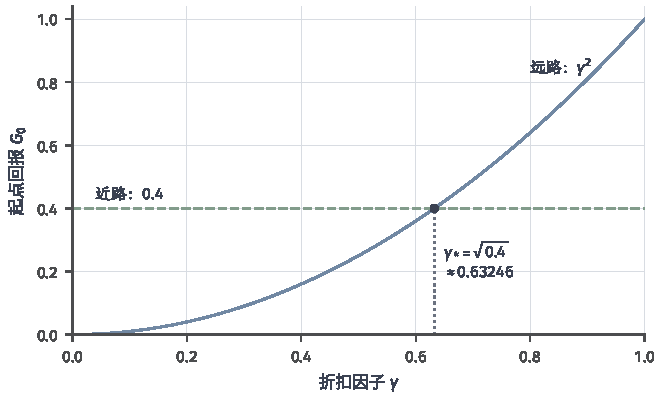
\includegraphics[width=112.000mm]{figures/10-reinforcement-learning/01-problems-and-solving/matplotlib/rl-overview-discount.pdf}
  \caption{独立确定性岔路算例的折扣偏好。横轴为$\gamma$，纵轴为起点回报；近路奖励序列为$(0.4)$，远路为$(0,0,1)$，无其他奖励。交点由解析等式求出。}
  \label{fig:rl-overview-discount}
\end{figure}

累计范围也可能因为时间上限而改变，但要先判断上限来自任务还是采集器。若任务规定“十步内到达才得分”，第十步之后的奖励不属于目标，剩余步数应作为策略可读取的状态分量，终端价值按规则设为零。若任务持续运行，只是采集器最多记录十步，$s_{10}$之后的回报并未消失。我们可以用未来价值估计补齐未记录部分，这称为自举（bootstrapping），即用已有预测代替尚未观测的后果；也可以不补齐，但需承担式~\eqref{eq:rl-overview-tail}给出的截断误差。自举不能应用于本来就不计入目标的未来。区分真正终止与采样截断，要依据任务规则，而不能只看一个含混的结束标记。

即使累计方式明确，奖励也可能鼓励我们不希望看到的行为。另设一个确定性导航任务，保留$\gamma=0.9$、原步成本和终点奖励，但增加一条两步循环。起点可以沿五步路径到达终点，也可以不断循环；到达路径不经过奖励路标，循环每步却都因经过路标多得$0.2$。循环每步净得$0.16$，无限循环的回报为$0.16/(1-0.9)=1.6$，超过五步到达的$0.51854$。这个算例取消了滑移并新增了循环，不是基准网格的精确解。选择循环可能完全符合给定奖励，却违背到达目标的意图。辅助奖励要在促进学习的同时保持最优策略不变，需要额外条件，第~\ref{chap:rl-reward}章再讨论。

奖励符合收益意图后，按期望比较仍有边界。设一个策略的回报必为$1$，另一个以各一半概率得$3$或$-1$；二者期望相同，后者却有一半概率出现负结果。平均数不能恢复失败概率、极端损失或不可违反的条件。第~\ref{chap:rl-trustworthy}章将分别讨论怎样评价回报分布、允许环境发生哪些扰动，以及行为必须满足哪些安全约束；把惩罚系数调大，不能自动给出这些保证。

% Outline: 1.1.6
\subsection{价值}
\label{sec:rl-overview-values}

% Outline: 1.1.6.1
\subsubsection{状态价值、动作价值与优势}
\label{sec:rl-overview-value-functions}

前面的轨迹算例都是在奖励串已经给定之后才算回报，但真正做决策时，我们并不知道这一步会走向哪条轨迹——既可能顺利到达，也可能因滑移偏离。要在动作尚未执行时就比较不同选择，就必须对所有可能的未来取平均。\term{价值函数}（value function）用条件期望承担这件事：固定环境、长期目标和今后遵循的策略，回答“平均而言能拿到多少回报”。这里又分两种问法。状态价值（state value）$V^\pi(s)$问的是“从状态$s$出发、包括当前动作在内都按策略$\pi$选择，平均回报是多少”；动作价值（action value）$Q^\pi(s,a)$则把当前这一步固定下来，问“从$s$出发先强制执行动作$a$、此后再按$\pi$行动，平均回报是多少”。后者专门用于比较同一个状态下的不同候选动作，因而在决策时更直接。两者之差$Q^\pi(s,a)-V^\pi(s)$称为\term{优势}（advantage），衡量“此刻特意改选动作$a$”相对于“按当前策略的平均方式行动”，平均能多拿或少拿多少回报。

\begin{definition}[状态价值、动作价值与优势]
  \label{def:rl-overview-values}
  设时间齐次MDP的奖励满足$|r_t|\leq R_{\max}<\infty$，折扣因子$0\leq\gamma<1$，$\pi$为合法平稳策略。从指定状态启动的轨迹期望定义折扣状态价值和动作价值：
  \begin{equation}
  \begin{aligned}
    V^\pi(s)&=\mathbb E_\pi[G_t\mid s_t=s],\\
    Q^\pi(s,a)&=\mathbb E_\pi[G_t\mid s_t=s,a_t=a].
  \end{aligned}
  \label{eq:rl-overview-values}
  \end{equation}
  条件事件有正概率时，以上采用通常的条件期望。对任意状态$s$，第一式按从$s$启动并遵从$\pi$定义；对任意合法动作$a$，第二式按从$s$启动、强制执行$a$、随后遵从$\pi$定义。因此，状态不必在原初始分布下可达，动作也不必满足$\pi(a\mid s)>0$。优势定义为
  $A^\pi(s,a)=Q^\pi(s,a)-V^\pi(s)$。
  有限时域或非平稳策略需要保留$V_t^\pi,Q_t^\pi,A_t^\pi$的时间下标。
\end{definition}

要从各动作的价值恢复策略在该状态的价值，需要把当前动作选择也平均进去。候选动作来自$\mathsf A(s)$，权重由固定策略给出，而不是在这里挑选最大值。下面沿有限或可数动作的点质量$\pi(a\mid s)$写成求和；一般动作空间上应改为对策略核$\pi(\mathrm da\mid s)$积分。由全期望公式，
\begin{equation}
  V^\pi(s)=\sum_{a\in\mathsf A(s)}\pi(a\mid s)Q^\pi(s,a).
  \label{eq:rl-overview-vq}
\end{equation}
优势用$V^\pi(s)$作共同基线。将其定义代入这个动作平均，再利用合法动作的概率和为$1$，得到
\[
  \sum_a\pi(a\mid s)A^\pi(s,a)
  =\sum_a\pi(a\mid s)Q^\pi(s,a)-V^\pi(s)=0.
\]
正优势表示相对于\emph{当前策略在该状态的平均行为}更好，并不表示相对于最优行为已经足够好，也不表示每次执行都会成功。

\begin{example}[随机网格中的两步价值]
  \label{ex:rl-overview-values}
  为了手算一次行动前的比较，保留基准网格全部转移与奖励，只将目标改为两步有限时域$H=2$，$\gamma=0.9$，$V_2=0$。从$c=(3,3)$开始，时刻$1$在$c$选右，在$(3,2)$选上，在$(2,3)$选右；其他状态任选合法动作，不影响以下计算。时刻$1$只剩一步，因此各处价值就是该步的期望奖励：
  \[
  \begin{aligned}
    V_1^\pi(c)&=0.792,& V_1^\pi((3,2))&=-0.04,\\
    V_1^\pi(g)&=0,& V_1^\pi((2,3))&=-0.04.
  \end{aligned}
  \]
  当前选右，以$0.8$到终点，以$0.1$留在$c$，以$0.1$到$(3,2)$。第一步期望奖励为$0.792$；第二步的期望回报按后继概率平均，再折扣一次，故
  \[
    Q_0^\pi(c,\text{右})
     =0.792+0.9[0.1(0.792)+0.1(-0.04)]=0.85968.
  \]
  当前选左时，以$0.8$到$(2,3)$，以$0.1$因向上滑移留在$c$，以$0.1$到$(3,2)$。三种后果都未到终点，所以即时期望奖励仍为$-0.04$；第二步分别使用这三个后继状态的$V_1^\pi$。

  当前选下时，以$0.8$到$(3,2)$，以$0.1$到$(2,3)$，另以$0.1$侧滑进入终点。即时奖励因而以$0.1$概率为$1$、以$0.9$概率为$-0.04$，平均为$0.064$。到终点那一支的后续价值是$V_1^\pi(g)=0$，第二步只需保留另两支的非零贡献。将各分支代入，得到
  \[
  \begin{aligned}
    Q_0^\pi(c,\text{左})
      &=-0.04+0.9[0.8(-0.04)+0.1(0.792)+0.1(-0.04)]\\
      &=-0.00112,\\
    Q_0^\pi(c,\text{下})
      &=0.1(1)+0.9(-0.04)+0.9[0.8(-0.04)+0.1(-0.04)]\\
      &=0.03160.
  \end{aligned}
  \]
  向下式中的第一个$0.9$是未进入终点的概率，方括号外的$0.9$则是折扣因子；两者数值相同，作用不同。该动作也可能因侧滑取得终点奖励，所以不能把它的即时期望误写成$-0.04$。若$\pi_0$以$0.5$选右、$0.25$选左、$0.25$选下，则
  \[
    V_0^\pi(c)=0.5(0.85968)+0.25(-0.00112)+0.25(0.03160)
              =0.43746.
  \]
  三个动作的优势依次为$0.42222,-0.43858,-0.40586$，按这些概率加权恰好为零。
\end{example}

图~\ref{fig:rl-overview-values}将这组数值放回格点，中心是当前策略的平均价值，箭头旁则是固定首动作的价值及其相对基线。只把$\pi_0$改为必选右，后续规则不变，三个$Q_0$也不变，但$V_0$变为$0.85968$。再把时刻$1$在$c$的选择改为左，就有$V_1(c)=-0.04$，当前向右的价值也变为$0.792+0.9[0.1(-0.04)+0.1(-0.04)]=0.7848$。这个对照分别改变了当前动作分布和后续策略，说明价值取决于环境、时间目标与策略，不是格子固有的属性。

\begin{figure}[htbp]
  \centering
  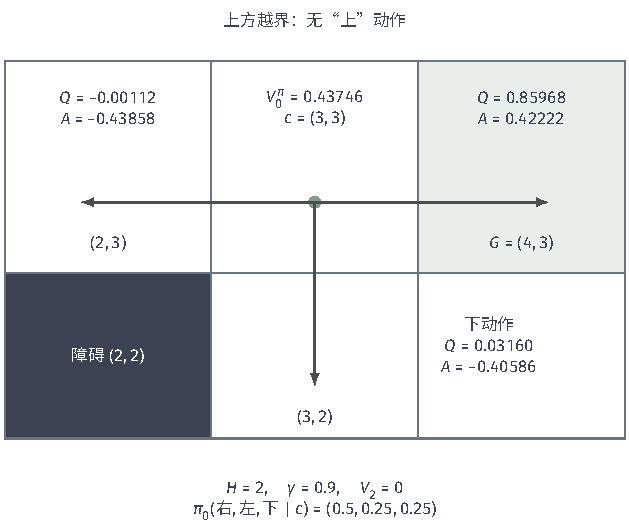
\includegraphics[width=106.581mm]{figures/10-reinforcement-learning/01-problems-and-solving/tikz/rl-overview-values.pdf}
  \caption{两步算例在$c=(3,3)$的价值分解。中心为$V_0^\pi$，三个合法意图方向标出$Q_0^\pi$与$A_0^\pi$；上方越界，因而没有上动作。全部数值对应示例~\ref{ex:rl-overview-values}，不是无限时域最优价值。}
  \label{fig:rl-overview-values}
\end{figure}

回到本章默认的无限时域折扣目标，固定时间齐次环境、合法平稳策略$\pi$与初始分布$\mu_0$，仍假设奖励有界且$0\leq\gamma<1$。在这组条件下，除按初始状态平均$V^\pi$外，还可以由策略诱导的状态动作分布计算同一个$J(\pi)$。逐时分布$q_t^\pi(s,a)$告诉我们时刻$t$遇到每种状态动作的概率，$R(s,a)$给出对应的平均奖励；两者相乘再求和，就是该时刻的期望评分。对时刻加折扣权重，便恢复总目标。有界奖励使级数绝对可和，允许交换期望与求和，得到
\begin{equation}
\begin{aligned}
  J(\pi)
   &=\mathbb E_{s_0\sim\mu_0}V^\pi(s_0)
     =\sum_{t\geq0}\gamma^t\sum_{s,a}q_t^\pi(s,a)R(s,a)\\
   &=\frac{1}{1-\gamma}\sum_{s,a}d^\pi(s,a)R(s,a).
\end{aligned}
\label{eq:rl-overview-objective-occupancy}
\end{equation}
最后一行用$d^\pi$汇总时间权重，但它比原来的折扣和多乘了$1-\gamma$，所以恢复$J$时必须除以这一系数。这把“策略去哪里、做什么”与“那些行为得到多少奖励”联系起来；后续占用分布的梯度和误差界须沿用同一归一化约定。

前面的两步算例仍使用$V_0^\pi$与有限时域回报，不能直接套用这里无时间下标的平稳价值。若要将两步任务补成无限记录，必须在第二步之后停止计奖，并保留剩余时间或相应的时间下标；这样扩展记录不会改变原来的两步目标。

% Outline: 1.1.6.2
\subsubsection{回报的递归关系}
\label{sec:rl-overview-bellman}

在两步算例中，我们先算最后一步、再把它带回当前一步。自然要问：能否用同样的“从后往前”方式处理任意长的未来，而不必逐条枚举所有轨迹？先对折扣回报本身做一次拆分。它的第一项就是当前奖励$r_t$，其余每一项都含一个共同的$\gamma$，对绝对收敛的级数可以把这个因子提到求和号外，于是得到一个不依赖任何近似的恒等式：
\begin{equation}
  G_t=r_t+\gamma G_{t+1}.
  \label{eq:rl-overview-return-recursion}
\end{equation}
有限时域下也有同样关系，只是末端为$G_{H,H}=0$。这个等式的含义很直观：从$t$起的总分，等于眼下拿到的$r_t$，加上从下一步起的总分$G_{t+1}$整体打一次折扣。恒等式本身解决了“分解”，真正的难点在于右边的$G_{t+1}$此刻尚未发生、仍是随机量，需要把它转换成可以计算的条件期望。

当前固定$s_t=s,a_t=a$后，下一步奖励和状态仍然随机。先对可能的$r_t,s_{t+1}$分情况，再评价从后继状态继续行动的回报：马尔可夫性使环境未来只依赖$s_{t+1}$，平稳策略使未来选择也只依赖后续状态。因此，
$\mathbb E_\pi[G_{t+1}\mid s_t,a_t,r_t,s_{t+1}]=V^\pi(s_{t+1})$。
先将回报分解代入动作价值，再用条件期望的塔式法则把未来回报分层平均：
\[
\begin{aligned}
 Q^\pi(s,a)
 &=\mathbb E_\pi[r_t+\gamma G_{t+1}\mid s_t=s,a_t=a]\\
 &=\mathbb E_\pi\!\left[
 r_t+\gamma\mathbb E_\pi[G_{t+1}\mid
 s_t,a_t,r_t,s_{t+1}]
 \,\middle|\,s_t=s,a_t=a\right]\\
 &=\mathbb E_\pi[r_t+\gamma V^\pi(s_{t+1})
                 \mid s_t=s,a_t=a].
\end{aligned}
\]
内层平均评价指定后继状态之后的未来，外层平均则按当前动作可能产生的奖励与后继状态计权。被替换的是$G_{t+1}$的内层条件期望，不是将每条轨迹上的随机回报都设为同一个数。有限或可数的状态与奖励下，将外层平均展开为联合概率的加权和，得到
\begin{equation}
  Q^\pi(s,a)=\sum_{s',r}p(s',r\mid s,a)
                         [r+\gamma V^\pi(s')].
  \label{eq:rl-overview-bellman-qv}
\end{equation}
该式把当前动作的价值变成一步反馈与后继状态价值的平均。用式~\eqref{eq:rl-overview-vq}平均当前动作，可得到$V^\pi$的递推；用同一式替换后继$V^\pi$，可得到$Q^\pi$的递推。

两式称为\term{Bellman期望关系}（Bellman expectation equations），它们都在评价固定策略，平均权重来自策略与环境，而不是对动作求最优：
\begin{align}
 V^\pi(s)
  &=\sum_a\pi(a\mid s)
        \left[R(s,a)+\gamma\sum_{s'}T(s'\mid s,a)V^\pi(s')\right],
        \label{eq:rl-overview-bellman-v}\\
 Q^\pi(s,a)
  &=R(s,a)+\gamma\sum_{s'}T(s'\mid s,a)
          \sum_{a'}\pi(a'\mid s')Q^\pi(s',a').
        \label{eq:rl-overview-bellman-q}
\end{align}
从联合核改写成$T,R$时，分别平均$r_t$和后继价值，只使用了期望的线性性，不要求二者独立。网格奖励恰好由后继状态决定，仍可使用这两式。递推现在给出了计算关系，但还需核对它计算的确实是原来定义的回报期望。有限时域可以从零终端值逐步往前验证；无限时域则需用尾项界控制有限截断与完整回报的差。

\begin{theorem}[回报期望与递推一致]
  \label{thm:rl-overview-recursion}
  设MDP的状态与动作均有限，各允许动作集合非空，$\pi$为合法马尔可夫策略序列。给定整数时域$H\geq1$及$0\leq\gamma\leq1$，每个时刻、每个合法状态动作的奖励绝对可积，终端价值为零。按$V_H^\pi=0$及
  \begin{equation}
    V_t^\pi(s)=\sum_a\pi_t(a\mid s)
      \int_{S\times\mathbb R}
      [r+\gamma V_{t+1}^\pi(s')]
      p_t(\mathrm d s',\mathrm d r\mid s,a)
    \label{eq:rl-overview-finite-recursion}
  \end{equation}
  反向计算，得到的量等于$\mathbb E_\pi[G_{t,H}\mid s_t=s]$。这里允许环境核$p_t$随时刻变化；时间齐次时$p_t=p$。
  对时间齐次模型、固定平稳策略、有界奖励与$0\leq\gamma<1$，无限折扣回报的条件期望满足式~\eqref{eq:rl-overview-bellman-v}和式~\eqref{eq:rl-overview-bellman-q}。
\end{theorem}

\begin{proof}
  与价值定义相同，零概率条件事件处采用从指定状态启动的含义。有限时域在$t=H$无剩余奖励，两边都为零。假设时刻$t+1$的递推值已经等于剩余回报的条件期望。将$G_{t,H}=r_t+\gamma G_{t+1,H}$代入，再按动作、奖励和后继状态逐层取条件期望，得到
  \[
  \begin{aligned}
   &\mathbb E_\pi[G_{t,H}\mid s_t=s]\\
   &\quad=\sum_a\pi_t(a\mid s)
      \int_{S\times\mathbb R}
      \bigl[r+\gamma\mathbb E_\pi[G_{t+1,H}\mid s_{t+1}=s']\bigr]\\
   &\qquad\qquad{}\times p_t(\mathrm d s',\mathrm d r\mid s,a).
  \end{aligned}
  \]
  内层条件期望只需$s_{t+1}$，是因为模型在给定时刻满足马尔可夫性，未来采用指定的策略序列。代入归纳假设就得到式~\eqref{eq:rl-overview-finite-recursion}。由$t=H-1$逐次归纳到$t=0$，有限结论成立。固定当前动作而不平均$\pi_t$，同一论证给出有限时域的$Q_t^\pi$关系。

  对无限折扣情形，令$V^{\pi,[n]}(s)$为从$s$开始只累加前$n$步的回报期望，方括号表示截断长度而非更新迭代。由已经证明的有限结论，
  \[
    V^{\pi,[n]}(s)=\sum_a\pi(a\mid s)
       \left[R(s,a)+\gamma\sum_{s'}T(s'\mid s,a)
                                       V^{\pi,[n-1]}(s')\right].
  \]
  式~\eqref{eq:rl-overview-tail}给出对所有$s$一致的界
  $|V^{\pi,[n]}(s)-V^\pi(s)|\leq\gamma^nR_{\max}/(1-\gamma)$，
  因而左边收敛到$V^\pi(s)$。右边加权平均的差至多为
  $\gamma\cdot\gamma^{n-1}R_{\max}/(1-\gamma)$，也趋于零，故极限满足式~\eqref{eq:rl-overview-bellman-v}。对固定首动作的截断回报重复同样步骤，得到式~\eqref{eq:rl-overview-bellman-qv}；再用动作平均关系替换其中的$V^\pi$，即得到式~\eqref{eq:rl-overview-bellman-q}。
\end{proof}

证明从回报定义出发，先验证有限递推，再用尾项界过渡到无限回报，因此没有用递推本身假定价值存在。但“价值满足这些式子”还不能反过来说明只有这一个函数满足它们，也不能说明反复计算右侧会收敛。不动点唯一性与计算误差由第~\ref{chap:rl-planning}章补足。

图~\ref{fig:rl-overview-backup}将式中的两层平均分开：先按策略选择动作，再按环境生成后继。若不再按当前策略平均，而是在合法动作中选择期望累计回报最大的一个，问题就从评价这份策略转为改进行为。最大值的候选集合是$\mathsf A(s)$，比较指标是动作的期望回报；这一新的求解问题也由规划章展开。

\begin{figure}[htbp]
  \centering
  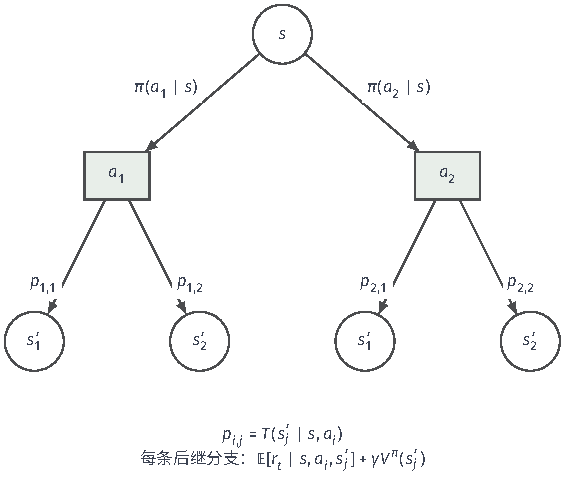
\includegraphics[width=95.617mm]{figures/10-reinforcement-learning/01-problems-and-solving/tikz/rl-overview-backup.pdf}
  \caption{Bellman期望备份的两层随机性。圆节点表示状态，方节点表示动作；第一层以$\pi(a\mid s)$平均，第二层以$T(s'\mid s,a)$平均后继价值。给定状态动作的即时奖励平均为$R(s,a)$；若按后继分支同时计入奖励，需保留奖励与后继状态的条件关系。}
  \label{fig:rl-overview-backup}
\end{figure}

% Outline: 1.2
\section{强化学习的研究内容}
\label{sec:rl-overview-research}

同一个网格任务可以提出不同问题：已有策略的回报怎样，怎样找到更好的策略，以及应当去哪里收集训练样本。回答这些问题，需要同时说明求解目标、环境访问权限和评价依据。

% Outline: 1.2.1
\subsection{核心研究问题}
\label{sec:rl-overview-questions}

给定一份策略，估计它的长期回报，称为\term{策略评价}（policy evaluation）；选择或改进策略以提高期望回报，称为\term{控制}（control）。当环境规律未知时，还需要\term{探索}（exploration）：主动尝试动作，取得能够区分候选动作后果的训练样本。探索可能牺牲当前回报，换取以后作出更好决策的依据。

求解可以沿两条路线进行。基于模型（model-based）方法显式利用环境的转移与奖励规律；规律未知时，先从交互记录估计环境模型，再据此规划。无模型（model-free）方法直接从训练样本估计价值或调整策略。这里的“模型”特指预测环境后果的模型，因此用神经网络表示价值函数仍可以是无模型方法。

图~\ref{fig:rl-overview-research-flow}展示这些路线怎样接入交互过程。价值估计帮助改进策略，环境模型支持预测与规划，新策略又改变后续训练样本的分布。晚到的奖励怎样评价早先动作、怎样表示复杂观测，以及更新能否稳定，都是这些路线共同面对的问题。

\begin{figure}[htbp]
  \centering
  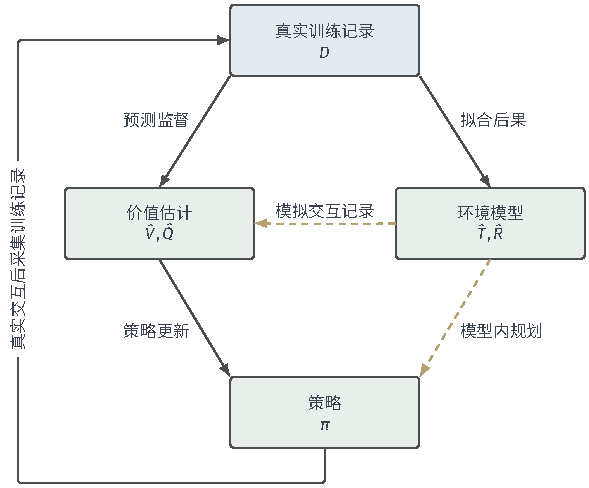
\includegraphics[width=99.815mm]{figures/10-reinforcement-learning/01-problems-and-solving/tikz/rl-overview-research-flow.pdf}
  \caption{训练样本、价值估计、环境模型与策略之间的依赖。实线表示真实交互记录参与模型拟合、价值估计及策略更新；虚线表示利用学习模型规划或生成模拟交互记录。各条路线可以组合使用。}
  \label{fig:rl-overview-research-flow}
\end{figure}

% Outline: 1.2.2
\subsection{问题边界与变体}
\label{sec:rl-overview-protocols}

环境模型是否已知，首先决定了求解任务。转移与奖励规律已知时，主要困难是在多步选择中控制计算量和近似误差，第~\ref{chap:rl-planning}章介绍动态规划与搜索。规律未知时，还需从有限训练样本估计动作后果，并协调探索与策略改进，第~\ref{chap:rl-learning}章介绍蒙特卡罗、时序差分、策略梯度和环境模型学习。

模型未知时，训练样本的采集权限也有不同设定。在线学习通常要沿实际轨迹到达某个状态，才能尝试该处的动作；\term{生成模型}（generative model）允许指定合法状态动作对，查询随机后继状态和奖励样本；离线学习只能使用固定日志。随机查询不等于知道精确转移概率，在线交互也不自动允许任意重置。有限批次交互则只在规定轮次内追加训练样本。

模型与采集权限之外，观测、奖励和任务要求也会改变问题。表~\ref{tab:rl-overview-variants}列出主要设定及后续章节的处理路线。观测不完整造成的是当前状态难以辨认，固定日志造成的是部分动作后果缺少训练样本，两者需要分别处理。

\begin{table*}[htbp]
  \centering\small
  \begin{tabularx}{\linewidth}{@{}>{\raggedright\arraybackslash}p{24mm}*{2}{>{\raggedright\arraybackslash}X}@{}}
    \toprule
    问题设定 & 主要困难 & 方法与承接位置\\
    \midrule
    观测不完整 & 同一观测可能对应不同状态，单次观测可能遗漏决策依据 & 根据交互历史推断状态，利用记忆或主动探测；第~\ref{chap:rl-information}章\\
    训练样本固定 & 待评价或改进的策略可能选择日志未覆盖的动作，无法补采其后果 & 离策略评价、行为约束与保守价值估计；第~\ref{chap:rl-information}章\\
    缺少可信奖励 & 缺少可信的标量奖励反馈，示范或偏好也未必唯一确定目标 & 行为克隆、逆强化学习、奖励建模与反馈校验；第~\ref{chap:rl-reward}章\\
    任务发生变化 & 目标、动力学或观测机制改变，旧策略未必仍然适用 & 共享表示、任务推断与元学习；第~\ref{chap:rl-transfer}章\\
    多个决策者 & 动作后果取决于共同选择，其他参与者也可能在学习 & 联合决策建模、集中训练与分散执行、自我对弈；第~\ref{chap:rl-multi-agent}章\\
    风险或安全受限 & 平均回报之外，还需控制严重失败、动力学扰动下的回报损失与约束违反 & 风险敏感优化、鲁棒规划、约束优化与安全过滤；第~\ref{chap:rl-trustworthy}章\\
    \bottomrule
  \end{tabularx}
  \caption{强化学习的主要问题变体。各行改变不同条件，可以在同一任务中同时出现；相应方法的保证仍依赖具体的观测、训练样本覆盖和环境假设。}
  \label{tab:rl-overview-variants}
\end{table*}

奖励受限还需区分两种情形。已经观测到随机奖励、只是其均值未知，属于通常的未知模型设定。\term{奖励无关探索}（reward-free exploration）则先在不知道奖励函数时收集转移记录，之后取得完整且有界的奖励函数，再用这些固定记录规划，不再追加交互。它要为全部允许的后续奖励保留足够覆盖，与从示范或偏好中学习奖励不同；相关协议见第~\ref{sec:rl-learning-guarantees-access}节。

这些设定可以叠加。例如，机器人可能只看到局部货架，只能用旧仓库日志训练，到新仓库后还须与其他机器人协作并避免碰撞。组合方法时，需要重新核对每一种限制下的适用条件。

% Outline: 1.2.3
\subsection{评价与研究证据}
\label{sec:rl-overview-evidence}

评价应与研究目标对应。价值估计关注预测与真实价值的误差，控制关注策略的期望回报，探索还需计入收集训练样本的代价。减少真实交互次数可能需要更多模型内计算，因此真实环境转移次数、模型查询次数与计算时间应分别报告。

评价训练完成后的策略时，应先固定策略和测试协议，再用未参与训练与候选选择的独立评价样本估计回报。任务目标、评价初始分布和时间范围必须一致。多个评价回合反映同一策略回报的随机波动，多次独立训练则反映学习过程的波动；两者都需要报告。任务外泛化还应单列新任务的适应预算，安全研究则需另报失败或约束违反情况。

定理说明假设成立时可以保证什么，受控实验考察具体设置下的方法作用，跨任务评价检验结果能延伸到哪些任务。三类证据相互补充，结论都应保持在各自的假设与评价范围内。

% Outline: 1.3
\section{强化学习的研究历史}
\label{sec:rl-overview-history}

强化学习逐步连接了三个问题：怎样根据结果改变行为，怎样规划多阶段行动，以及怎样从连续经验学习长期预测。随着表示能力和计算规模扩大，研究又进入高维观测、连续控制和更复杂的交互设定。

% Outline: 1.3.1
\subsection{强化学习的思想源流}
\label{sec:rl-overview-origins}

一种行为得到某种结果后，以后还会不会再被选择？Thorndike在早期行为研究及1911年的专著中讨论效果律（law of effect），将情境、行为与后果联系起来，为试错学习提供了思想线索。当时尚无本章的MDP与折扣目标框架\scite{rl1-thorndike1911-learning}。

动态与目标已知时，困难在于怎样安排一系列行动。Bellman的动态规划把长期决策分解为后继子问题，用后继价值比较当前选择，建立了递归求解的基础\scite{rl1-bellman1957-dp}。对于从经验改善预测的问题，Samuel的跳棋程序探索了局面评价的学习；程序仍利用已知棋局规则与搜索\scite{samuel1959}。

终局结果出现很晚时，还可以利用相邻时刻的预测来学习。Sutton在1988年的工作中系统讨论\term{时序差分}（temporal difference, TD）预测，用一步奖励和后继价值预测修正当前预测，使长期评价可以逐步更新\scite{rl1-sutton1988-td}。图~\ref{fig:rl-overview-history}将这些线索及相关代表工作放在同一时间线上。

\begin{figure*}[htbp]
  \centering
  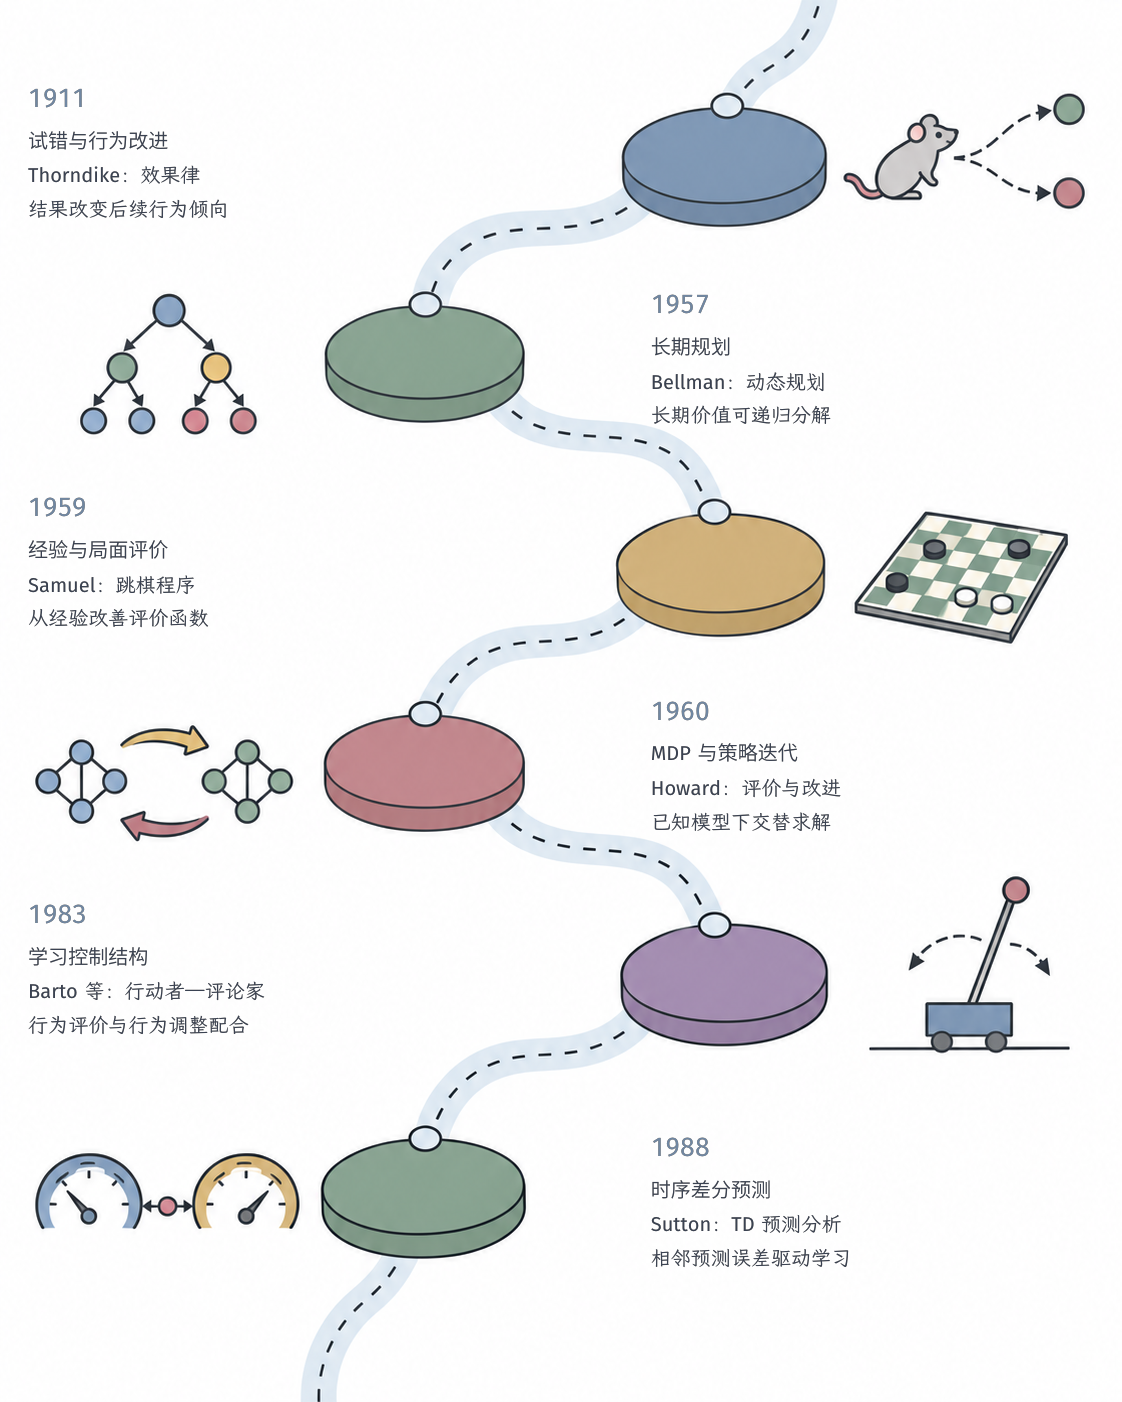
\includegraphics[width=157.400mm,height=.88\textheight,keepaspectratio]{figures/10-reinforcement-learning/01-problems-and-solving/generated/rl-overview-history/figure.png}
  \caption{强化学习思想源流的代表工作。沿曲线路径从上向下按年代阅读，节点间距不按年份等比例缩放；年份对应正文所引代表文献，路径不表示直接因果继承或方法替代。}
  \label{fig:rl-overview-history}
\end{figure*}

% Outline: 1.3.2
\subsection{现代强化学习框架的形成}
\label{sec:rl-overview-modern}

MDP使已知模型下的规划与未知模型下的学习能够围绕同一长期目标讨论。Howard在1960年的专著中系统发展了MDP的动态规划与策略迭代，交替评价当前策略并据此改进，形成了已知模型下的重要求解路线\scite{rl1-howard1960-dp}。

模型未知时，蒙特卡罗评价用采样回报估计价值，TD则利用一步经验和已有预测构造更新目标。前者在有限时域任务中可以等到轨迹结束，后者缩短了等待，但目标也受价值预测误差影响。把评价接到行为调整上，\term{行动者—评论家}（actor--critic）让评论家估计长期后果，再据此更新行动者的动作分布；Barto、Sutton与Anderson在1983年的学习控制工作中研究了这种配合结构\scite{rl1-barto1983-control}。

Q-learning直接估计最优动作价值，通过比较后继状态的候选动作来形成学习目标。Watkins于1989年提出该方法，Watkins与Dayan在1992年给出限定条件下的收敛证明，条件包括表格表示、充分访问和适当步长\scite{rl1-watkins1992-qlearning}。这些方法将价值学习与行为改进连接起来，具体更新及其成立条件见第~\ref{chap:rl-learning}章。

% Outline: 1.3.3
\subsection{函数逼近与规模扩展}
\label{sec:rl-overview-approximation}

连续位置、速度和关节角无法逐点存入价值表，高维离散状态的组合数也会迅速增长。函数逼近用共享参数计算价值或动作分布，使有限训练样本能够影响多个状态的预测。近似动态规划研究怎样在这种受限表示下计算价值并改进策略，Bertsekas与Tsitsiklis的神经动态规划专著系统连接了动态规划、仿真与函数逼近\scite{rl1-bertsekas1996-ndp}。

策略也可以直接用参数表示，再沿期望回报上升的方向调整参数，这就是策略梯度的基本思路。Williams在1992年研究的REINFORCE用采样回报加权动作对数概率的导数，估计策略梯度，无须对环境动态求导；这类估计的抽样波动也推动了后续的方差控制研究\scite{rl1-williams1992-reinforce}。

参数共享带来泛化，也带来状态间的相互干扰。利用后继预测修正当前预测称为自举，使用其他策略采集的训练样本学习称为离策略学习。函数逼近与这两种机制结合时，更新可能发散，表格方法的收敛结论不能直接推广到任意网络。第~\ref{chap:rl-learning}章将展开这些机制及稳定学习的条件。

% Outline: 1.3.4
\subsection{深度强化学习的兴起}
\label{sec:rl-overview-deep}

根据游戏画面选择动作，需要同时学习观测表示与长期价值。深度Q网络（deep Q-network, DQN）将卷积网络与动作价值学习结合，并用经验回放复用交互记录、用目标网络减缓学习目标的变化。2015年的Atari游戏结果展示了这种组合处理高维视觉观测的能力\scite{mnih2015}。

连续控制难以枚举全部候选动作。深度确定性策略梯度（deep deterministic policy gradient, DDPG）用行动者直接给出连续动作，再由评论家估计动作价值并指导行动者更新，将深度方法扩展到模拟物理控制\scite{rl1-lillicrap2016-ddpg}。

对于规则已知、可进行前瞻模拟的围棋，AlphaGo的2016年系统结合策略网络、价值网络与蒙特卡罗树搜索，用模拟对局分配搜索预算，以网络指导候选落子和局面评价，并通过人类棋谱及自我对弈训练\scite{silver2016}。这些进展分别利用了表示学习、策略优化和搜索；游戏或仿真中的成功仍须结合相应的模型访问与交互条件理解。

% Outline: 1.3.5
\subsection{研究范围的拓展}
\label{sec:rl-overview-expansion}

研究也逐步处理完整状态与可信奖励难以取得的任务。部分可观测决策根据历史观测推断隐藏状态，Kaelbling、Littman与Cassandra在1998年的工作系统讨论了相应规划框架\scite{rl1-kaelbling1998-pomdp}。目标难以直接写成奖励时，则可利用示范或人类反馈；Christiano等在2017年用人类对轨迹片段的偏好训练奖励预测，再据此学习策略\scite{christiano2017}。

多个决策者与行为约束也有长期研究基础。Shapley在1953年研究随机博弈，将状态转移与多个参与者的共同决策联系起来；约束MDP则在回报目标之外另设成本预算，Altman的专著系统处理了这类问题\scite{rl1-shapley1953-games,rl1-altman1999-cmdp}。这些方向改变的是观测、目标或参与者等问题条件，其方法与后文章节的对应关系已在表~\ref{tab:rl-overview-variants}中列出，并不构成深度强化学习之后才依次出现的年代阶段。

% Outline: 1.3.6
\subsection{前沿研究方向}
\label{sec:rl-overview-frontiers}

跨任务研究希望复用已有训练结果，减少新任务所需的训练样本。Gato用统一序列组织多种任务的观测和动作编码，通过监督式序列训练学习共享参数\scite{rl1-reed2022-gato}。共享编码仍需对齐具体任务的观测与动作含义，不能使不同机器人的动作编号自动互换。

进一步的上下文强化学习把已有或新增的观测、动作和奖励记录作为决策依据，在参数固定时调整后续行为。可扩展上下文Q学习（S-ICQL）从这些交互记录估计动作价值，再据此生成策略，Vintix II研究多领域决策预训练及上下文适应\scite{rl1-liu2026-sicql,rl1-polubarov2026-vintix}。在线适应可以取得新反馈，离线推断只能使用给定记录；两者的交互预算与适用任务范围需要分别评价，相关机制见第~\ref{chap:rl-transfer}章。

另一条路线先学习可供决策使用的\term{世界模型}（world model），即根据观测和给定动作预测后继变化与任务反馈的环境模型。DreamerV3在模型预测的想象轨迹中训练策略，TD-MPC2在每次决策时利用学习模型规划，Dreamer 4探索由固定离线记录训练模型并在模型内学习行为\scite{rl1-hafner2025-dreamerv3,rl1-hansen2024-tdmpc2,rl1-hafner2025-dreamer4}。图~\ref{fig:rl-overview-world-loop}展示模型内求解怎样接回真实环境：预测轨迹中的高回报仍需真实评价，旧轨迹上的预测准确也不保证未尝试动作的后果预测准确。

\begin{figure}[htbp]
  \centering
  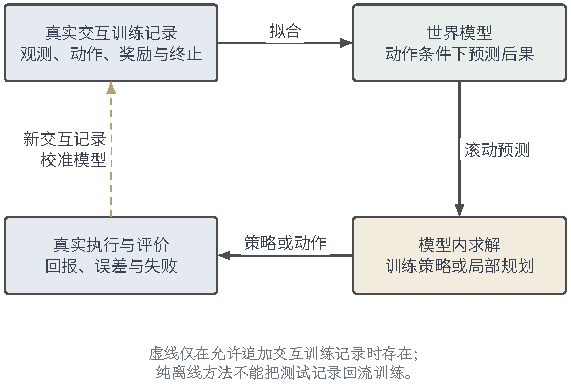
\includegraphics[width=96.615mm]{figures/10-reinforcement-learning/01-problems-and-solving/tikz/rl-overview-world-loop.pdf}
  \caption{可供决策使用的世界模型闭环。实线连接训练样本、模型内求解与独立评价；虚线校准路径只在允许追加真实训练记录时存在。模型预测的回报需要在真实环境中检验。}
  \label{fig:rl-overview-world-loop}
\end{figure}

工具使用把动作扩展为检索、运行程序或修改文件等调用，面临长程信用分配和局部观测的困难。Agent Lightning将执行程序与策略训练分开，保存实际调用记录，再据此更新语言模型策略；其后续版本进一步对齐训练采样与实际运行流程\scite{rl1-luo2025-lightning,rl1-he2026-lightning}。一次工具调用与语言模型生成的一个词元对应不同的动作尺度，任务成功率也须在相同工具权限和调用预算下比较。

要进一步回答“若主动改选动作会怎样”，还需要区分预测与因果识别。观察日志中的关联未必确定干预结果，即使各动作的转移分布已知，也未必能够回答同一次具体经历若换一个动作会怎样；相关区分可参考\BookChapterRef{chap:causal-inference}{卷2《数学准备：概率、因果与决策》中讨论因果响应的章节}。Oberst与Sontag用结构因果模型构造反事实轨迹，所得解释依赖所指定的生成机制\scite{rl1-oberst2019-counterfactual}。跨任务复用这类机制时，还须明确哪些关系保持不变，以及已有观察或干预记录是否足以确定所求结果。

% Outline: 1.4
\section{本章小结}
\label{sec:rl-overview-summary}

回到网格任务，决策问题现在有了可核算的说明。状态是除障碍外的格子，合法命令按意图方向确定，环境以$0.8/0.1/0.1$执行或滑移；起点、终点吸收与奖励规则固定。给出一份策略，就能由动作概率与环境核计算轨迹概率，再用占用度量汇总折扣时间中的状态动作分布。回报给这些轨迹计长期总分，价值则在行动前按可能后果取平均。策略改变的既是长期回报，也是后续经验的来源。

章首的机器人因此不能只按当前距离选择动作：距离变小，并不能保证整段行动到达目标，更不能保证安全。比较行动需指定后继分布、长期评分和后续规则；从经验作出比较，还需检查训练样本是否覆盖待选行为的后果。本章给出了描述和评价这些关系的对象，尚未求出仓储任务的最优安全路线。表~\ref{tab:rl-overview-distinctions}用三个具体判断收拢易混对象，便于继续检查求解方法与实验结论。

\begin{table*}[htbp]
  \centering\small
  \begin{tabularx}{\linewidth}{@{}>{\raggedright\arraybackslash}p{31mm}>{\raggedright\arraybackslash}X@{}}
    \toprule
    区别 & 可用于检验理解的具体判断\\
    \midrule
    状态与观测 & 相同照片可能对应门已开或未开；照片不一定是充分状态。见第~\ref{sec:rl-overview-mdp}节。\\
    奖励样本与长期价值 & $(3,3)$向右的一次奖励是$1$或$-0.04$；两步$Q_0^\pi=0.85968$是多种未来的平均。见第~\ref{sec:rl-overview-value-functions}节。\\
    行为与目标策略 & 日志始终向左，不代表待评价策略也应向左；右行的后果仍可能缺证据。见第~\ref{sec:rl-overview-occupancy}节。\\
    \bottomrule
  \end{tabularx}
  \caption{对象不同，能够回答的问题也不同。数值判断沿用本章明确给出的两步算例，不能移作无限时域结论。}
  \label{tab:rl-overview-distinctions}
\end{table*}

有界奖励与$0\leq\gamma<1$保证了折扣回报存在，也给出截断尾项界；有限时域和无限折扣下的条件期望论证则说明价值满足递推。价值存在和满足递推，还不意味着已经有可承受的求解方法，也不意味着有限训练样本能估计得足够准。第~\ref{chap:rl-planning}章先在模型可访问时建立规划与计算误差基准，区分精确期望和指定查询点的随机采样；第~\ref{chap:rl-learning}章再处理未知环境中的经验收集、估计与策略改进。历史和前沿中的方法虽然扩展了表示与接口，结论仍须绑定评价目标、观测机制和训练样本采集权限，因为行动始终同时改变结果与学习证据。

\chapter{给定模型下的规划}
\label{chap:rl-planning}

第~\ref{chap:rl-overview}~章用随机滑移的网格说明了为何要比较动作的长期后果，也证明了回报期望满足Bellman递推。本章把问题进一步收紧：假设导航模型已经给出，我们能够查询每个合法动作会把机器人带向何处、得到什么奖励。于是待求的对象不再是“环境规律是什么”，而是“怎样利用已知规律算出一份好策略”，这类在给定模型上求解最优或近似最优行为的工作统称为规划（planning）。

即使规律全部已知，规划仍有计算上的困难。一次查询只涉及一个状态动作，可一份策略必须应对机器人后续可能到达的许多状态；把所有后果枚举出来、为每个状态保存价值、以及把价值算到所需精度，都要消耗计算、存储与查询资源。本章的主线就是考察：在给定的资源预算下，怎样把“一步查询”组织成对整段未来的评价。

在进入方法前，还要先弄清“模型已经给出”到底允许我们取得什么答案，因为不同的允许方式对应不同的算法与代价。给定一个后继价值估计$v$，要比较当前动作，需要计算当步期望奖励与折扣后继价值之和。\term{精确期望访问}（exact expectation access）允许直接计算
$R(s,a)+\gamma\sum_{s'}T(s'\mid s,a)v(s')$；网格模型若明确列出了向前和向两侧滑移的全部概率，就能按概率逐项加权求和。\term{生成模型访问}（generative model access）则弱得多：它只允许指定任意合法的$(s,a)$，再取得一个独立样本$(r,s')\sim p(\cdot,\cdot\mid s,a)$，相当于反复调用一个模拟器。重复同一查询可能返回不同后果，规划器只能用样本均值估计上述期望。

生成模型无须公开概率表，也不要求规划器先从起点走到$s$；它提供的是从指定查询点正确采样的能力。因此，模型准确并不意味着有限次查询已经给出准确期望。本章把两种接口都作为给定资源，在各方法中分别说明所需能力。尤其不能把真实机器人的交互默认成生成模型：机器人通常只能从当前位置继续行动，不能任意重置到待查状态。后面的稀疏采样规划依赖这种指定查询点的能力\scite{rl2-kearns2002-sparse}

我们先沿用前章的有限折扣MDP：状态、动作集合有限，每个$\mathsf A(s)$非空，$|r_t|\leq R_{\max}$，且$0\leq\gamma<1$。奖励$r_t$仍按执行$a_t$的时刻编号，价值和策略性能仍是未归一化折扣回报。前章的有界回报结论于是给出$|V^\pi(s)|\leq V_{\max}:=R_{\max}/(1-\gamma)$。讨论有限时域、成本最小化或平均奖励时，我们会在当地重新规定目标，避免把这些设定混入折扣结论。

在这些条件下，本章按“预算从充足到紧张”的顺序组织求解方式。若计算与存储都充足，Bellman动态规划逐状态使用递推，全局优化则同时约束所有状态动作；这是两条求解同一目标的一般精确路线。若动力学、成本或子任务之间还存在额外结构，有时能显著减少精确求解所需的未知量或动作比较，但每一种简化都必须逐项验证其条件是否成立。若状态数或搜索树仍超出预算，还剩两条近似路线：只为当前状态展开局部后果，或保存一份跨状态复用的近似价值；局部搜索又可以借助这份近似价值评估未展开的未来，因此两类近似能够配合。图~\ref{fig:rl-planning-map}~展示的正是这些求解方式及其联系，后文再用误差和资源要求逐一比较它们。

\begin{figure*}[htbp]
  \centering
  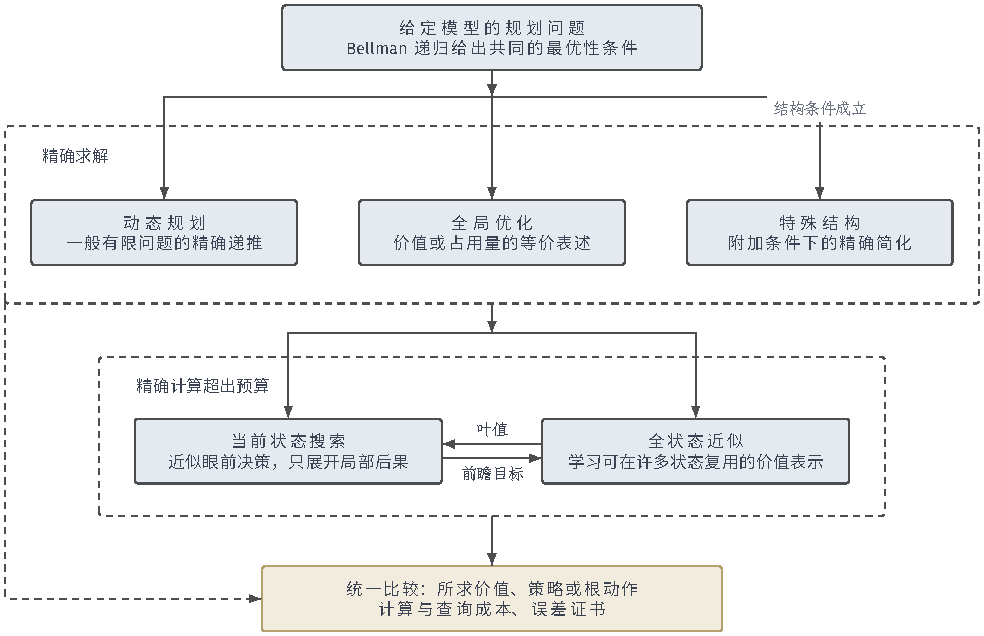
\includegraphics[width=166.617mm]{figures/10-reinforcement-learning/01-problems-and-solving/tikz/rl-planning-map.pdf}
  \caption{给定模型时的规划方法关系。动态规划与全局优化是一般精确路线；特殊结构只在附加条件成立时给出精确简化。精确计算超出预算后，可以近似当前决策或构造全状态近似，二者可通过叶节点价值与前瞻目标结合。}
  \label{fig:rl-planning-map}
\end{figure*}

% Outline: 2.1
\section{Bellman动态规划}
\label{sec:rl-planning-dp}

在网格的一个岔路口，若已经知道各后继状态的价值，就能用“当步奖励加折扣后继价值”比较各个合法方向，而不必把这些方向之后的全部轨迹重新枚举一遍。动态规划（dynamic programming）反复利用这种一步分解：先求出较短未来的价值，再用它算出较长未来的价值，逐步得到原先难以直接计算的长期价值。本节分三步走：先固定一条动作规则、只算遵从它的后果（策略评价），再用评价结果比较其他动作（策略改进），最后把动作选择直接并入价值更新（价值迭代）。

% Outline: 2.1.1
\subsection{策略评价}
\label{sec:rl-planning-evaluation}

给定平稳策略$\pi$，策略评价要算的是从每个状态出发遵从它的$V^\pi$，这一步并不重新选择动作，动作概率完全由给定的$\pi$决定。为把前章的Bellman关系整理成可以求解的线性方程，先把当步奖励和转移概率都按$\pi$平均：
\[
 r^\pi(s)=\sum_a\pi(a\mid s)R(s,a),\qquad
 T^\pi(s,s')=\sum_a\pi(a\mid s)T(s'\mid s,a).
\]
这样得到的$r^\pi$是按$\pi$行动时的当步期望奖励，并非一次模拟实际拿到的数值；$T^\pi$描述“遵从$\pi$时”下一状态的分布，它把动作选择的随机性和环境转移的随机性合在了一起。在精确期望接口下，按状态排列的$\bm r^\pi$和$\bm T^\pi$都可以直接算出，整张表里唯一未知的就是价值向量。令$\bm v^\pi$的$s$坐标为$V^\pi(s)$，Bellman方程便写成
\begin{equation}
 \bm v^\pi=\bm r^\pi+\gamma\bm T^\pi\bm v^\pi,\qquad
 (\bm I-\gamma\bm T^\pi)\bm v^\pi=\bm r^\pi.
 \label{eq:rl-planning-linear-evaluation}
\end{equation}
矩阵$\bm T^\pi$非负且每行之和为1，其无穷范数（最大绝对行和）为1。这意味着$\|\gamma\bm T^\pi\|_\infty=\gamma<1$：每多向前递推一层，未来的贡献就要再打一次折扣。于是矩阵几何级数$\sum_{k\geq0}\gamma^k(\bm T^\pi)^k$收敛到$(\bm I-\gamma\bm T^\pi)^{-1}$，评价方程因而有唯一解，而且可以直接写出来。矩阵范数和逆矩阵级数的结论可参考\BookChapterRef{chap:linear-analysis}{卷1《数学准备：计算、分析与几何》中“谱和奇异值”章}。这个级数解还有一层直观含义：把它乘开后，第$k$项$\gamma^k(\bm T^\pi)^k\bm r^\pi$恰好是第$k$步的折扣期望奖励，所以“解线性方程”和“按时间把各步期望奖励累加起来”得到的是同一个$V^\pi$。

\begin{example}[三个格子的独立手算模型]
 \label{ex:rl-planning-corridor}
 为看清线性方程如何计入反复停留，我们另设一条$x,y,g$三格走廊，从$x$开始。它不是宽4、高3基准网格的局部转移表：非终点只有“前进”和“等待”，前进以$0.8$进入下一格、以$0.2$留在原处，等待则必定原地不动，不再有侧向滑移。$g$保留零奖励吸收动作。进入$g$仍得1，其余非终点步仍得$-0.04$，并取$\gamma=0.9$。

 固定总是前进的策略，按$x,y,g$排序有
 \[
 \bm T^\pi=
 \begin{pmatrix}0.2&0.8&0\\0&0.2&0.8\\0&0&1\end{pmatrix},
 \qquad
 \bm r^\pi=\begin{pmatrix}-0.04\\0.792\\0\end{pmatrix}.
 \]
 在$y$前进只有$0.8$概率进入终点，所以第二个期望奖励为$0.8\times1+0.2\times(-0.04)=0.792$，不是每次都得1。终点以后没有奖励，故$V^\pi(g)=0$；把原地停留项移到左侧，得到
 \[
 0.82V^\pi(y)=0.792,\qquad
 0.82V^\pi(x)=-0.04+0.72V^\pi(y),
 \]
 因而
 \[
 V^\pi(y)=\frac{198}{205}\approx0.965854,\qquad
 V^\pi(x)=\frac{6718}{8405}\approx0.799286.
 \]
 也可以从$v^{(0)}=0$开始，每轮都用上一轮的整张表计算新值。前两轮在$(x,y)$处依次得到
 $(-0.04,0.792)$与$(0.52304,0.93456)$。这种同步备份第一轮只计当步奖励，第二轮才把$y$处的已有价值传到$x$。
\end{example}

走廊中的同步计算可以推广到所有状态：\term{Bellman备份}（Bellman backup）用已有的后继价值重算当前状态的一步期望，相当于对整张价值表统一“刷新”一次。为表示对整张表做一次备份，定义策略算子
\begin{equation}
 (\mathcal B^\pi v)(s)=r^\pi(s)+\gamma\sum_{s'}T^\pi(s,s')v(s').
 \label{eq:rl-planning-policy-operator}
\end{equation}
这个算子读入一张价值表$v$、输出一张新表，所以它作用的对象是“整份价值函数”，而不是某个数值。随之产生两个对实践很重要的问题：反复备份会不会收敛？初值取得不好会不会影响最终答案？我们用无穷范数衡量两张表的最大状态误差（在所有状态中取绝对误差的最大值），把再次备份后完全不再改变的价值表称为不动点。数学上，非空完备度量空间上的压缩自映射有唯一不动点，且从任意初值反复作用都会收敛到它；这里需要核对的是Bellman算子是否满足压缩性、压缩因子又是多少。一般结论和停止误差工具可参考\BookChapterRef{chap:metric-spaces}{卷1《数学准备：计算、分析与几何》的“度量空间”章}。

\begin{theorem}[策略评价的压缩性与收敛]
 \label{thm:rl-planning-policy-contraction}
 设MDP的状态集$S$与各非空动作集$\mathsf A(s)$有限，联合核时间齐次，奖励满足$|r_t|\leq R_{\max}<\infty$，且$0\leq\gamma<1$。固定合法平稳策略$\pi$，则$\mathcal B^\pi:\mathbb R^{|S|}\to\mathbb R^{|S|}$在无穷范数下为$\gamma$压缩映射，其唯一不动点为$V^\pi$。同步迭代$v^{(k+1)}=\mathcal B^\pi v^{(k)}$满足
 \[
 \lVert v^{(k)}-V^\pi\rVert_\infty
 \leq\gamma^k\lVert v^{(0)}-V^\pi\rVert_\infty.
 \]
\end{theorem}
\begin{proof}
 对任意$v,u$和状态$s$，期望奖励相消，故
 \[
 \begin{aligned}
 |(\mathcal B^\pi v)(s)-(\mathcal B^\pi u)(s)|
 &\leq\gamma\sum_{s'}T^\pi(s,s')|v(s')-u(s')|\\
 &\leq\gamma\lVert v-u\rVert_\infty.
 \end{aligned}
 \]
 第一个不等式来自概率非负，第二个来自概率之和为1：加权平均不会放大最大坐标差。对$s$取最大值，便说明备份把两张表的距离缩至原来的至多$\gamma$倍，这就是压缩性。有限维实向量空间在此范数下完备，压缩映射定理保证唯一不动点和迭代收敛。前章已由回报分解证明$V^\pi$满足式~\eqref{eq:rl-planning-policy-operator}，因此不动点就是所求价值。每轮把$v^{(k)}$与$V^\pi$代入压缩不等式，连续使用$k$次即得误差界。
\end{proof}

迭代界还含未知的初始真实误差。实际计算时，我们更容易检查一张表再次备份后改变了多少；这项变化也能控制它离$V^\pi$还有多远。

\begin{theorem}[评价残差证书]
 \label{thm:rl-planning-evaluation-residual}
 设状态动作有限、动作集非空、奖励有界且$0\leq\gamma<1$的时间齐次MDP，$\pi$为合法平稳策略，$V^\pi$为其折扣价值。对任意$v:S\to\mathbb R$，
 \begin{equation}
 \lVert v-V^\pi\rVert_\infty
 \leq\frac{\lVert \mathcal B^\pi v-v\rVert_\infty}{1-\gamma}.
 \label{eq:rl-planning-evaluation-residual}
 \end{equation}
\end{theorem}
\begin{proof}
 插入$\mathcal B^\pi v$并利用不动点关系，有
 \[
 \begin{aligned}
 \lVert v-V^\pi\rVert_\infty
 &\leq\lVert v-\mathcal B^\pi v\rVert_\infty+
       \lVert \mathcal B^\pi v-\mathcal B^\pi V^\pi\rVert_\infty\\
 &\leq\lVert v-\mathcal B^\pi v\rVert_\infty+
       \gamma\lVert v-V^\pi\rVert_\infty.
 \end{aligned}
 \]
 将右边的真实误差项移到左侧，再除以正数$1-\gamma$，就把未知价值误差界在了可计算的备份差之内。
\end{proof}

这项备份差称为\term{Bellman残差}（Bellman residual）：$\mathcal B^\pi v-v$在每个状态上度量“当前预测”与“Bellman递推要求它等于的值”之间还差多少。它的价值在于完全可计算——只要模型已知就能直接算出来，无须事先知道真实的$V^\pi$；而定理把这个看得见的量与看不见的真实误差联系了起来。要让每个状态的价值误差都不超过$\varepsilon$，只需确认全状态残差的无穷范数不超过$(1-\gamma)\varepsilon$，这给出了一个可以随时检查的停机标准。需要注意，只抽查少量状态、或用样本去估计残差，都不能直接给出同样的全状态证书，必须另外控制未查状态和采样估计带来的误差。

同步备份要求所有状态都使用同一轮的旧值、整轮结束后才一起更新，这需要同时保存新旧两张表。Gauss--Seidel更新则按固定顺序逐个覆盖：后更新的状态可以立刻使用本轮刚算出的较新后继值，因而往往收敛得更快；异步更新更灵活，允许一次只处理一部分状态。不过这种便利附带条件：对精确备份，收敛的一个充分条件是每个状态都被无限次更新，且所用的后继价值估计不会永久停留在旧迭代轮次上，有界延迟是常用的更强条件。证明思路是把“所有状态都完成一次有效更新”划分为一个阶段，逐阶段压低覆盖全状态的误差上界。实际中优先处理残差大的状态通常能节省工作量，但不能因此跳过某些状态——被遗漏状态的误差会一直留在那里、并传给把它作为后继的前驱状态。标准处理可参见Sutton与Barto教材第4章\scite{sutton2018}。

% Outline: 2.1.2
\subsection{策略改进与迭代}
\label{sec:rl-planning-policy-iteration}

有了$V^\pi$，可以重新检查网格中的方向选择。向左绕回起点与向终点移动，当步奖励可能同为$-0.04$，长期后果却不同。我们先只改变当前这一步，以后仍遵从$\pi$；这样既能比较新动作，又能沿用刚算出的后继价值：
\[
 Q^\pi(s,a)=R(s,a)+\gamma\sum_{s'}T(s'\mid s,a)V^\pi(s').
\]

目标是提高期望折扣回报，因此我们在合法集合$\mathsf A(s)$中选择$Q^\pi$最大的动作。

\begin{definition}[贪心策略]
 \label{def:rl-planning-greedy}
 给定有限MDP中的合法平稳策略$\pi$及其有限实数动作价值$Q^\pi$。相对于$Q^\pi$的贪心策略是在每个状态$s$将全部概率放在最大化动作集合中的合法平稳策略，该集合为
 \[
  \arg\max_{a\in\mathsf A(s)}Q^\pi(s,a)
 \]
 确定性选择在每个状态取一个最大化动作，随机选择可以在这些动作间分配任意概率。策略迭代采用确定性规则：若旧动作仍达到最大值，就保留旧动作；否则按预先固定次序选一个最大化动作。
\end{definition}

这样的“贪心”比较里包含了折扣后的未来回报，并非只挑即时奖励最大的动作，这也是它与第~\ref{chap:rl-overview}~章网格中“只看当步$-0.04$无法区分方向”的关键区别。但还有一件事必须证明，不能想当然：$Q^\pi$只衡量了“当前这一步偏离$\pi$、以后又回到$\pi$”的效果，为什么据此在每个状态都改选最好动作、得到一份全新策略后，真实价值仍不会下降？这正是策略改进定理要回答的问题。

\begin{theorem}[策略改进及策略迭代的有限终止]
 \label{thm:rl-planning-policy-improvement}
 设MDP的状态动作有限、动作集非空、奖励有界、联合核时间齐次，且$0\leq\gamma<1$，$\pi,\pi'$为合法平稳策略。若$\mathcal B^{\pi'}V^\pi\geq V^\pi$逐状态成立，则$V^{\pi'}\geq V^\pi$。从确定性平稳策略开始，每轮精确评价并逐状态选择最大动作价值；旧动作仍并列最大时保留，否则按固定次序选取一个最大化动作。这样的策略迭代在有限轮后终止于对所有初始状态最优的策略。
\end{theorem}
\begin{proof}
 非负转移概率保证备份保持逐状态大小关系：$u\geq v$就有$\mathcal B^{\pi'}u\geq \mathcal B^{\pi'}v$，这称为算子的单调性。对假设中的不等式反复使用同一个$\mathcal B^{\pi'}$，
 \[
 V^\pi\leq \mathcal B^{\pi'}V^\pi
 \leq (\mathcal B^{\pi'})^2V^\pi\leq\cdots.
 \]
 定理~\ref{thm:rl-planning-policy-contraction}~说明右端收敛到$V^{\pi'}$，所以逐状态不等式在极限中仍成立。

 贪心改进满足
 $\mathcal B^{\pi'}V^\pi\geq \mathcal B^\pi V^\pi=V^\pi$。若策略改变，保留并列旧动作的规则保证至少某个状态$s$有
 $(\mathcal B^{\pi'}V^\pi)(s)>V^\pi(s)$；上述单调序列又说明
 $V^{\pi'}(s)\geq(\mathcal B^{\pi'}V^\pi)(s)>V^\pi(s)$。
 因此策略未终止时，价值向量至少一个坐标严格增加，其他坐标不减，不可能回到以前的策略。确定性平稳策略至多有$\prod_s|\mathsf A(s)|$个，故必在有限步停止。

 有限终止还不够，我们必须检查终止策略是否支配所有允许的行为。停止意味着旧动作已是最大化动作，所以对于所有$s,a$，
 \[
 V^\pi(s)\geq R(s,a)+\gamma\sum_{s'}T(s'\mid s,a)V^\pi(s').
 \]
 对任意可能依赖历史的策略$\sigma$，将该不等式沿它的动作与转移取条件期望并连续展开$H$步，得到
 \[
 V^\pi(s)\geq
 \mathbb E_\sigma\!\left[
 \sum_{t=0}^{H-1}\gamma^t r_t+\gamma^H V^\pi(s_H)
 \,\middle|\,s_0=s\right].
 \]
 有界价值乘$\gamma^H$后趋于0，故$H\to\infty$时有$V^\pi(s)\geq V^\sigma(s)$。这里没有把$\sigma$限制成平稳或确定性策略；它任意而$\pi$自身可行，因而终止策略在所有状态最优。
\end{proof}

下面的算法将确定性策略核简记为合法动作映射$\pi^{(k)}(s)$：这个值是在状态$s$以概率1选择的动作，等价的策略核在该动作处取1、其余动作处取0。

\begin{algorithm}[精确策略迭代]
 \label{alg:rl-planning-policy-iteration}
 \begin{algorithmic}[1]
  \Require 精确模型，$\gamma<1$，确定性初始策略$\pi^{(0)}$
  \Ensure 全状态最优确定性平稳策略
  \For{$k=0,1,\ldots$}
   \State 解$(\bm I-\gamma\bm T^{\pi^{(k)}})\bm v=\bm r^{\pi^{(k)}}$
   \For{每个状态$s$}
    \State 计算$q(s,a)=R(s,a)+\gamma\sum_{s'}T(s'\mid s,a)v(s')$
    \State 在最大化动作中保留旧动作，否则按固定次序选取$\pi^{(k+1)}(s)$
   \EndFor
   \If{$\pi^{(k+1)}=\pi^{(k)}$}
    \State \Return $\pi^{(k)}$
   \EndIf
  \EndFor
 \end{algorithmic}
\end{algorithm}

算法~\ref{alg:rl-planning-policy-iteration}~把上述证明对应的评价与改进组成一个循环。为观察不同位置怎样先后改变动作，我们回到未简化的基准网格：起点$(1,1)$、终点$(4,3)$、障碍$(2,2)$，意图方向概率$0.8$、两侧滑移各$0.1$；非法意图方向被排除，滑移撞墙仍留在原处。表~\ref{tab:rl-planning-grid-pi}~按“左、下、右、上”取每个状态第一个合法动作为$\pi^{(0)}$，并使用同一次序处理需要换动作的并列选择，列出两轮精确评价和改进。终点仅有零奖励吸收动作，故省略其行。

\begin{table*}[htbp]
 \centering
 \small
 \begin{tabularx}{\linewidth}{@{}c*{3}{c}*{3}{>{\raggedright\arraybackslash}X}@{}}
  \toprule
  状态 & $\pi^{(0)}$ & $\pi^{(1)}$ & $\pi^{(2)}$ &
  $V^{\pi^{(0)}}$ & $V^{\pi^{(1)}}$ & $V^{\pi^{(2)}}$\\
  \midrule
  $(1,1)$ & 右 & 右 & 右 & $-0.400000$ & $0.393318$ & $0.395377$\\
  $(2,1)$ & 左 & 右 & 右 & $-0.400000$ & $0.515595$ & $0.517970$\\
  $(3,1)$ & 左 & 右 & 右 & $-0.398373$ & $0.642761$ & $0.645466$\\
  $(4,1)$ & 左 & 上 & 上 & $-0.383549$ & $0.769713$ & $0.771194$\\
  $(1,2)$ & 下 & 下 & 下 & $-0.400000$ & $0.296572$ & $0.298380$\\
  $(3,2)$ & 下 & 右 & 上 & $-0.383549$ & $0.785763$ & $0.801271$\\
  $(4,2)$ & 左 & 上 & 上 & $-0.246674$ & $0.948042$ & $0.949576$\\
  $(1,3)$ & 下 & 下 & 右 & $-0.400000$ & $0.268198$ & $0.606648$\\
  $(2,3)$ & 左 & 右 & 右 & $-0.400000$ & $0.783647$ & $0.784994$\\
  $(3,3)$ & 左 & 右 & 右 & $-0.398373$ & $0.948042$ & $0.949576$\\
  \bottomrule
 \end{tabularx}
 \caption{基准随机网格的两轮策略改进。每列价值均解完整线性方程后四舍五入至六位小数，不是轨迹样本均值。$\pi^{(2)}$尚未声称最优，下一轮仍需重新检查贪心条件。}
 \label{tab:rl-planning-grid-pi}
\end{table*}

初始策略把左侧区域封闭起来，进入后会一直付出步成本，因此这些状态的价值为$-0.04/(1-0.9)=-0.4$。第一轮已使$(2,1)$转向右，$(1,3)$却仍保留向下：在旧策略的评价中，右邻还会把机器人带回左侧。第二轮用改进后的后继价值重算，才使$(1,3)$转向右。这说明后续行为的改善如何传到前面的选择，也说明一次改进未必足以恢复最终路线。

为在同一模型下比较完整策略，再定义\term{均匀合法策略}$\pi_{\mathrm u}$：每个非终点状态在$\mathsf A(s)$内等概率选择，即$\pi_{\mathrm u}(a\mid s)=1/|\mathsf A(s)|$；非法方向概率为0，终点只选择零奖励吸收动作。比较仍取$\mu_0((1,1))=1$、$\gamma=0.9$，进入终点得1，其余非终点步得$-0.04$，不改滑移规律。解式~\eqref{eq:rl-planning-linear-evaluation}~得到$J(\pi_{\mathrm u})\approx-0.154754$；将精确策略迭代继续到终止，再评价终止策略，得到$J(\pi^*)\approx0.421161$。这些数字四舍五入至六位小数，由配套网格程序用有理数线性消元计算，不是学习实验结果；二者的差别来自动作选择，而非环境或奖励改变。

每轮都把评价方程完整解到收敛可能很费计算，尤其在策略只是小幅改变时也要重解一遍。一个自然的折中是只做有限几次评价备份、就立刻用当前还不精确的价值改动作。表~\ref{tab:rl-planning-evaluation-schedules}~比较这种安排与精确评价，并说明修改策略迭代把部分评价放在循环的哪个位置。\term{广义策略迭代}（generalized policy iteration）概括“评价与改进反复相互影响”这一普遍配合关系；但它只是对这种配合的命名，并不保证任意不精确的交替都能让真实性能单调上升——评价欠准确时，贪心改进的方向也可能出错。

\begin{table}[htbp]
 \centering
 \small
 \begin{tabularx}{\linewidth}{@{}l>{\raggedright\arraybackslash}X>{\raggedright\arraybackslash}X@{}}
  \toprule
  安排 & 每次评价工作 & 何时改进\\
  \midrule
  精确评价 & 解方程；理论上也可迭代至极限 & 得到$V^\pi$后\\
  部分评价 & 固定若干次备份或达到指定残差 & 评价预算用尽时\\
  修改策略迭代 & 从当前$v$选贪心策略，再做$m_k\geq1$次该策略备份 & 每个外层循环一次\\
  \bottomrule
 \end{tabularx}
 \caption{评价深度与改进频率。部分评价是一类操作，修改策略迭代是将它嵌入明确循环的算法；两者不是互斥类别。}
 \label{tab:rl-planning-evaluation-schedules}
\end{table}

% Outline: 2.1.3
\subsection{价值迭代}
\label{sec:rl-planning-value-iteration}

策略迭代每一轮都要先把某份完整策略评价准确，才能改进一次。如果我们的最终目的只是尽快逼近最优价值、并不关心中间策略是否被评价充分，完全可以把“改进”这一步直接揉进每次备份：在重算每个状态时立刻比较所有合法动作，只保留“当步奖励加后继估值”中最大的那个结果。这样不再需要等待一整份策略被评价完，动作选择本身成为更新的一部分，这就是价值迭代的思路。

\begin{definition}[最优Bellman算子]
 \label{def:rl-planning-optimal-operator}
 给定有限状态动作、非空动作集、有限期望奖励$R(s,a)$及$0\leq\gamma<1$的时间齐次MDP。最优Bellman算子$\mathcal B^*:\mathbb R^{|S|}\to\mathbb R^{|S|}$对每个状态函数$v$作用为
 \begin{equation}
 (\mathcal B^*v)(s)=\max_{a\in\mathsf A(s)}
 \left\{R(s,a)+\gamma\sum_{s'}T(s'\mid s,a)v(s')\right\}.
 \label{eq:rl-planning-optimal-operator}
 \end{equation}
 相对于$v$的贪心策略$\pi_v$选择该式的最大化动作，因此$\mathcal B^{\pi_v}v=\mathcal B^*v$。
\end{definition}

\begin{theorem}[最优不动点与平稳最优策略]
 \label{thm:rl-planning-optimal-fixed-point}
 设时间齐次MDP的状态动作有限、各动作集非空、奖励有界，且$0\leq\gamma<1$。以$V^*(s)=\sup_\sigma V^\sigma(s)$表示从$s$启动、遍历所有合法历史依赖随机策略的最优折扣价值。则$\mathcal B^*$单调且在无穷范数下为$\gamma$压缩映射，其唯一不动点为$V^*$；存在合法确定性平稳策略$\pi^*$，使$V^{\pi^*}(s)=V^*(s)$对所有$s$成立。
\end{theorem}
\begin{proof}
 若$v\leq u$，每个动作的期望备份都不减，取最大值后仍有$\mathcal B^*v\leq \mathcal B^*u$。对有限个实数$\{f_a\},\{g_a\}$，取$f_a$的最大化动作$a_f$，有
 $\max_a f_a-\max_a g_a\leq f_{a_f}-g_{a_f}\leq\max_a|f_a-g_a|$。
 交换两组数便得最大值之差的绝对值界。因此
 \[
 \lVert \mathcal B^*v-\mathcal B^*u\rVert_\infty
 \leq\gamma\lVert v-u\rVert_\infty.
 \]
 压缩映射定理给出唯一不动点$\bar v$。有限动作集保证每个状态都能取到一个最大化动作，组成确定性平稳策略$\bar\pi$。于是
 $\mathcal B^{\bar\pi}\bar v=\mathcal B^*\bar v=\bar v$，策略评价不动点的唯一性给出$\bar v=V^{\bar\pi}$。

 还须证明$\bar v$不只是平稳策略中的某个值。不动点对每个动作给出
 $\bar v(s)\geq R(s,a)+\gamma\mathbb E[\bar v(s')\mid s,a]$。
 沿任意历史依赖随机策略逐步取条件期望，展开$H$步，
 \[
 \bar v(s)\geq\mathbb E\!\left[
 \sum_{t=0}^{H-1}\gamma^t r_t+\gamma^H\bar v(s_H)
 \,\middle|\,s_0=s\right].
 \]
 $\bar v$在有限状态集上有界，尾项趋于0，故$\bar v$支配每个策略的价值。另一方面$\bar\pi$实现它，因此$\bar v=V^*$，取$\pi^*=\bar\pi$即得结论。
\end{proof}

\term{价值迭代}（value iteration）反复执行$v^{(k+1)}=\mathcal B^*v^{(k)}$，用当前后继估值计算下一轮的最大一步备份。由压缩性，
$\lVert v^{(k)}-V^*\rVert_\infty\leq\gamma^k\lVert v^{(0)}-V^*\rVert_\infty$。
若不使用含初始误差的轮数界，也可以再次检查备份差。按评价残差证明插入$\mathcal B^*v$并移项，得到
\begin{equation}
 \lVert v-V^*\rVert_\infty
 \leq\frac{\lVert \mathcal B^*v-v\rVert_\infty}{1-\gamma}.
 \label{eq:rl-planning-optimal-residual}
\end{equation}
同步更新时，$v^{(k+1)}-v^{(k)}$恰好是旧表$v^{(k)}$的残差，因此其无穷范数能为旧表提供证书。若实际返回新表，则应检查新表的残差，或另行推导它的界；两张表对应的索引不能混用。

价值表接近$V^*$之后，最终仍要从表中读出动作并真正执行。这里要区分两类误差：表本身的预测误差$\|v-V^*\|$，与执行所选出的策略后真实回报与最优回报之差（策略损失）；后者才是我们最终关心的性能指标。由于一份近似表会在机器人实际运行时反复影响每一次动作选择，一个看似很小的单点误差可能在多步决策中被放大。下面的定理就把“全状态价值精度”换算成“长期执行贪心策略的性能损失”。

\begin{theorem}[由价值精度到贪心策略性能]
 \label{thm:rl-planning-greedy-loss}
 设状态动作有限、动作集非空、奖励有界、$0\leq\gamma<1$的时间齐次MDP，$V^*$为最优折扣价值。若$\varepsilon\geq0$、$v:S\to\mathbb R$满足$\lVert v-V^*\rVert_\infty\leq\varepsilon$，且合法平稳策略$\pi_v$仅选择$R(s,a)+\gamma\sum_{s'}T(s'\mid s,a)v(s')$的最大化动作，则
 \begin{equation}
 \lVert V^*-V^{\pi_v}\rVert_\infty
 \leq\frac{2\gamma\varepsilon}{1-\gamma}.
 \label{eq:rl-planning-greedy-loss}
 \end{equation}
\end{theorem}
\begin{proof}
 利用$\mathcal B^*v=\mathcal B^{\pi_v}v$，在$\mathcal B^*V^*-\mathcal B^{\pi_v}V^{\pi_v}$中插入这两个相等的量，有
 \[
 \begin{aligned}
 \lVert V^*-V^{\pi_v}\rVert_\infty
 &\leq\lVert \mathcal B^*V^*-\mathcal B^*v\rVert_\infty
       +\lVert \mathcal B^{\pi_v}v-\mathcal B^{\pi_v}V^{\pi_v}\rVert_\infty\\
 &\leq\gamma\varepsilon+
       \gamma\lVert v-V^{\pi_v}\rVert_\infty\\
 &\leq2\gamma\varepsilon+
       \gamma\lVert V^*-V^{\pi_v}\rVert_\infty.
 \end{aligned}
 \]
 第一项$\gamma\varepsilon$控制最优备份受到估值误差的影响，第二项再计入同一表与执行策略价值的差。将最后的策略损失移到左侧即得结论，因此该界覆盖反复执行$\pi_v$，而不只覆盖根动作。
\end{proof}

先用残差界控制价值误差，再代入贪心性能界，可知全状态最优残差为$\eta$时，精确贪心策略的损失至多
$2\gamma\eta/(1-\gamma)^2$。这也给出了按策略精度选择停止阈值的依据。若$\gamma=0$，未来不再计入目标，直接最大化即时奖励已精确最优，不需要含$1/\gamma$的阈值。

图~\ref{fig:rl-planning-grid-values}~固定基准网格和零初值，展示终点收益怎样随精确备份向远处传播。终点值始终为0，因为奖励1已经在进入它的那一步支付；若再把终点值设为1，就会重复计奖。第一轮邻近终点的最大期望奖励为$0.792$，更远状态则在后续轮次中才计入这项收益。

\begin{figure*}[htbp]
 \centering
 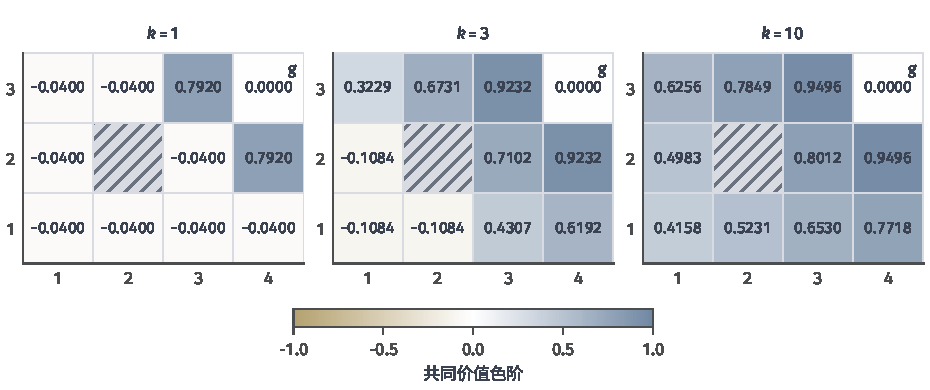
\includegraphics[width=157.400mm]{figures/10-reinforcement-learning/01-problems-and-solving/matplotlib/rl-planning-grid-values.pdf}
 \caption{基准随机网格在$k=1,3,10$次同步价值迭代后的价值，$\gamma=0.9$、$v^{(0)}=0$。数字由完整转移期望计算，显示四位小数；三个面板共用色阶，障碍单独标记。它们是确定的算法迭代值，不是实验学习曲线。}
 \label{fig:rl-planning-grid-values}
\end{figure*}

上述迭代和证书依赖折扣压缩性。若目标只计有限步，我们可以从指定终端值反向算，不需要令迭代趋于无限；若改用平均奖励，累计收益通常不断增长，原价值不动点也不再适用。表~\ref{tab:rl-planning-horizons}~对照这三种任务。平均奖励方程中的差分价值$h(s)$衡量扣除共同增长趋势后的状态差别；表中$T_ah(s)=\sum_{s'}T(s'\mid s,a)h(s')$。对所有状态同时给$h$加同一个常数，方程不变，但存在共同最优平均奖励$g$本身并不保证$h$仅有这种不确定性。例如两个互不连通的零奖励吸收状态都有$g=0$，它们的$h$却可各取任意值；固定其中一个状态的值仍不能确定另一个。参考状态归一化只消除整体常数，唯一性和迭代收敛还须另核结构条件。这些时间目标及其条件可见Puterman的系统论述\scite{rl1-puterman1994-mdp}

表中将用到的通信条件要求：对任意两个状态，都存在某份合法策略，使过程从前一个状态经有限步以正概率到达后一个状态；不同状态对可以使用不同策略。这是在允许选择策略后考察环境中的可达性。固定一份平稳策略后，它诱导的转移链是否不可约，或是否只有一个闭的常返类，则是另一层条件；后一种单链情形还允许暂态状态。通信并不要求每份策略都诱导不可约链，也不能单独保证任意相对价值迭代收敛，表中的迭代条件仍须分别核验。

\begin{table}[htbp]
 \centering
 \small
 \begin{tabularx}{\linewidth}{@{}l>{\raggedright\arraybackslash}X>{\raggedright\arraybackslash}X@{}}
  \toprule
  目标 & 递推与边界 & 关键条件与保证\\
  \midrule
  有限时域 & $V_H=0$，$V_t=\mathcal B_t^*V_{t+1}$；无折扣时取该式$\gamma=1$ & 反向做$H$层；策略一般随$t$变化\\
  无限折扣 & $V^*=\mathcal B^*V^*$ & 有限状态动作、奖励有界、$\gamma<1$；无穷范数压缩\\
  平均奖励 & $g+h(s)=\max_a\{R(s,a)+T_ah(s)\}$ & 需另给通信等条件以得到共同增益$g$；相对价值迭代收敛还需相应非周期或更强混合条件\\
  \bottomrule
 \end{tabularx}
 \caption{不同时间目标的递推口径。平均奖励相对价值迭代通常每轮减去参考状态的备份值来固定$h$的常数，但不能直接套用$\gamma<1$的证明。}
 \label{tab:rl-planning-horizons}
\end{table}

% Outline: 2.2
\section{从动态规划到全局优化}
\label{sec:rl-planning-linear-programming}

刚才的动态规划是逐状态备份、靠反复迭代收敛到最优价值。同一个有限折扣MDP还可以换一个角度：把所有状态动作“最终应满足的关系”一次性写成一组并行的约束，再交给一个优化器统一求解。未知量有两种自然选择：可以是各状态的价值，也可以是策略在折扣时间内分配给各状态动作的访问量。前者给出的约束限制了长期回报的上界，后者的约束则限定哪些访问分布真的能由某份策略实现。下面先分别建立这两个线性规划，再说明它们恰好构成一对互为对偶、最优值相同的问题。

% Outline: 2.2.1
\subsection{价值的线性规划}
\label{sec:rl-planning-value-lp}

最优Bellman方程说明：在状态$s$先取任意合法动作，再最优行动，回报都不能超过$V^*(s)$。我们据此要求候选函数$v$满足
$v(s)\geq R(s,a)+\gamma\sum_{s'}T(s'\mid s,a)v(s')$，对每个状态动作都成立。下一项证明将说明这些约束使$v$成为$V^*$的逐状态上界。既然上界可以任意抬高，我们应将它压低，而不是最大化它。用非负权重$w(s)$指定各状态在目标中的分量，目标和约束都关于$v$线性，得到线性规划（linear programming, LP）：
\begin{equation}
 \begin{aligned}
 \min_v\quad &\sum_s w(s)v(s)\\
 \text{满足}\quad
 &v(s)-\gamma\sum_{s'}T(s'\mid s,a)v(s')\geq R(s,a),
 \quad s\in S,\ a\in\mathsf A(s).
 \end{aligned}
 \label{eq:rl-planning-value-lp}
\end{equation}
式~\eqref{eq:rl-planning-value-lp}~在所有满足Bellman不等式的状态函数中，最小化加权价值。这里的$\min$寻找最紧的上界，并非把策略的回报改成最小化。每个合法动作都对应一条约束；若事先删除某个动作，其长期后果就不再受到检查，可能改变所求上界。

\begin{theorem}[价值线性规划的解]
 \label{thm:rl-planning-value-lp}
 设状态动作有限、动作集非空、奖励有界、$0\leq\gamma<1$的时间齐次MDP，权重$w(s)\geq0$。任意满足每个合法状态动作的Bellman不等式$v(s)\geq R(s,a)+\gamma\sum_{s'}T(s'\mid s,a)v(s')$的$v:S\to\mathbb R$，均逐状态满足$v\geq V^*$。若所有$w(s)>0$，则式~\eqref{eq:rl-planning-value-lp}的唯一最优解为$V^*$。
\end{theorem}
\begin{proof}
 因为每个动作的备份都不超过$v$，这些约束等价于$v\geq \mathcal B^*v$。利用单调性反复备份，
 $v\geq \mathcal B^*v\geq(\mathcal B^*)^2v\geq\cdots$，而压缩性使后者收敛到$V^*$，所以$v\geq V^*$。$V^*$自身满足全部约束，因而可行。对任何不同于$V^*$的可行$v$，至少一个坐标严格大于$V^*$，其他坐标不小于；所有权重严格为正便推出
 $\sum_s w(s)v(s)>\sum_s w(s)V^*(s)$。这同时证明最优性和唯一性。
\end{proof}

若只比较从$\mu_0$出发的回报，可以取$w=\mu_0$；所有约束仍然保留，但零权重状态未必得到唯一价值。例如在走廊之外增加不可达的孤立状态$z$，其唯一动作是零奖励自循环，约束只要求$v(z)\geq\gamma v(z)$，也就是$v(z)\geq0$。当$\mu_0(z)=0$时，任何这样的$v(z)$都不影响目标，而真正的$V^*(z)$为0。因此初始分布下目标已最优，仍不能推出每个坐标都等于全状态最优价值。

% Outline: 2.2.2
\subsection{占用度量的线性规划}
\label{sec:rl-planning-occupancy-lp}

换用访问量作变量时，最需要保证的是：所选的这组概率质量必须真的能由环境中的某份策略产生，而不能脱离动力学任意指派。先回顾第~\ref{chap:rl-overview}~章定义的归一化占用度量
\[
 d^\pi(s,a)=(1-\gamma)\sum_{t=0}^{\infty}
 \gamma^t\mathbb P_\pi(s_t=s,a_t=a),\qquad
 d^\pi(s)=\sum_a d^\pi(s,a).
\]
其中$d^\pi(s)$汇总折扣时间内落在$s$的概率质量。它一部分来自初始分布，另一部分由此前状态动作转移而来。拆出$t=0$项，再对其余时刻使用全概率公式，便得到这种流守恒关系：
\begin{equation}
 \begin{aligned}
 d^\pi(s)
 &=(1-\gamma)\mu_0(s)
   +(1-\gamma)\sum_{t=1}^{\infty}\gamma^t
     \sum_{x,a}\mathbb P_\pi(s_{t-1}=x,a_{t-1}=a)T(s\mid x,a)\\
 &=(1-\gamma)\mu_0(s)+\gamma\sum_{x,a}T(s\mid x,a)d^\pi(x,a).
 \end{aligned}
 \label{eq:rl-planning-flow}
\end{equation}
式~\eqref{eq:rl-planning-flow}~要求一个状态分配给各动作的总量，等于初始注入加折扣后的转移流入。图~\ref{fig:rl-planning-occupancy-flow}~把这两项放回三格走廊：注入为$(1-\gamma)\mu_0$，每条转移流还乘$\gamma$。对所有状态求和，并利用转移概率之和为1，可得
$\sum_{s,a}d^\pi(s,a)=1$。终点吸收后仍占用折扣时间，只是不再产生奖励。

\begin{figure}[htbp]
 \centering
 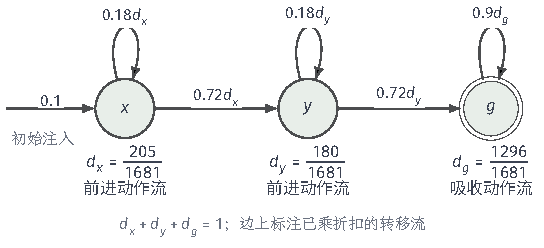
\includegraphics[width=92.050mm]{figures/10-reinforcement-learning/01-problems-and-solving/tikz/rl-planning-occupancy-flow.pdf}
 \caption{手算走廊中前进策略的归一化折扣流。状态流出分别为$d_x,d_y,d_g$；初始注入为$0.1$，前进转移流为$0.72d$，原地流为$0.18d$，终点吸收流为$0.9d_g$。等待动作在最优解中的流量为0，未画出。}
 \label{fig:rl-planning-occupancy-flow}
\end{figure}

这项流约束也会从价值线性规划的对偶中自然出现。取$w=\mu_0$，把每条价值约束写成“右端减左端不大于0”，再引入非负乘子$\lambda(s,a)$。乘子给各约束分配权重，拉格朗日函数把加权约束与原目标相加：
\[
 \begin{aligned}
 L(v,\lambda)
 &=\sum_s\mu_0(s)v(s)
 +\sum_{s,a}\lambda(s,a)[R(s,a)-v(s)]\\
 &\quad+\gamma\sum_{s,a}\lambda(s,a)\sum_xT(x\mid s,a)v(x)\\
 &=\sum_{s,a}\lambda(s,a)R(s,a)+\sum_s v(s)\kappa_\lambda(s),
 \end{aligned}
 \]
将含同一个$v(s)$的项收集后，其系数为
\[
 \kappa_\lambda(s)=\mu_0(s)-\sum_a\lambda(s,a)
       +\gamma\sum_{x,a}T(s\mid x,a)\lambda(x,a).
\]
对固定$\lambda$，取$\inf_v L(v,\lambda)$可为原最小化问题给出下界。由于$v(s)$可以取任意实数，若有一个系数$\kappa_\lambda(s)$非零，就能沿相反方向把$L$降到负无穷；只有全部系数为0才得到有限下界。这个条件正是注入为$\mu_0$的流方程，因而$\lambda$对应总质量为$1/(1-\gamma)$的\emph{未归一化}占用量。对偶在这些可行乘子中最大化下界；代入$d=(1-\gamma)\lambda$，得到
\begin{equation}
 \begin{aligned}
 \max_{d\geq0}\quad&
 \frac{1}{1-\gamma}\sum_{s,a}d(s,a)R(s,a)\\
 \text{满足}\quad&
 \sum_a d(s,a)-\gamma\sum_{x,a}T(s\mid x,a)d(x,a)
   =(1-\gamma)\mu_0(s),\quad s\in S.
 \end{aligned}
 \label{eq:rl-planning-occupancy-lp}
\end{equation}
对偶的$\max$也可以直接理解为：在满足流守恒的访问量中选取累计期望奖励最大的分布。归一化只改变变量尺度，目标仍是$J(\pi)$，所以流注入改为$(1-\gamma)\mu_0$后，目标中的$(1-\gamma)^{-1}$必须保留。接着要验证，这些代数上可行的流确实都对应合法策略。

\begin{theorem}[可行占用量的策略实现]
 \label{thm:rl-planning-occupancy-realization}
 设MDP的状态动作有限、各动作集非空、$0\leq\gamma<1$，初始分布为$\mu_0$。任意非负状态动作函数$d$，若满足对所有$s$的流约束$\sum_a d(s,a)-\gamma\sum_{x,a}T(s\mid x,a)d(x,a)=(1-\gamma)\mu_0(s)$，均可由合法平稳随机策略实现。具体地，令$d(s)=\sum_a d(s,a)$；在$d(s)>0$处取$\pi(a\mid s)=d(s,a)/d(s)$，在$d(s)=0$处任取合法动作分布，则$d=d^\pi$。
\end{theorem}
\begin{proof}
 在正占用状态，按比例选择动作直接给出$d(s,a)=d(s)\pi(a\mid s)$。在零占用状态，各动作量非负且和为0，只能全部为0，因此同一等式仍成立，不依赖该处选什么合法分布。代入流方程，并用列向量$\bm d$收集状态占用量，
 \[
 \bm d=(1-\gamma)\bm\mu_0+\gamma(\bm T^\pi)^\top\bm d.
 \]
 由于$\bm I-\gamma\bm T^\pi$可逆，其转置也可逆，此方程的唯一解为
 \[
 \bm d=(1-\gamma)\sum_{t=0}^{\infty}
 \gamma^t((\bm T^\pi)^\top)^t\bm\mu_0.
 \]
 右端正是策略$\pi$的折扣状态分布。再乘$\pi(a\mid s)$，得到$d(s,a)=d^\pi(s,a)$。零占用状态的任意动作选择没有改变这个唯一解。
\end{proof}

% Outline: 2.2.3
\subsection{价值与占用度量的对偶关系}
\label{sec:rl-planning-duality}

价值线性规划给回报设上界，占用线性规划选取可实现的访问分布；现在需要确认两种求法会不会留下间隙。价值问题可用常数$R_{\max}/(1-\gamma)$作为可行函数，目标又由$V^*$从下方界住。占用问题至少有任意平稳策略的流作为可行点；所有可行$d$非负、总质量为1，且奖励有界，故目标有界。有限维线性规划只要原问题可行且最优值有限，原问题和对偶问题都能达到相同的最优值。这里已核验价值与占用问题的可行性和有界性，因此两种规划的最优目标相等。该强对偶结论及互补松弛的依据可参考\BookChapterRef{chap:optimization}{卷1《数学准备：计算、分析与几何》中讨论最优化的章节}。

我们用示例~\ref{ex:rl-planning-corridor}~检验这种对应。两个非终点处，前进策略的价值都高于等待的一步备份$-0.04+0.9V(s)$，而前进备份恰好等于该价值，因此前进策略满足最优Bellman方程。取$\mu_0(x)=1$，对应流量满足
\[
 d_x=0.1+0.18d_x,\qquad
 d_y=0.72d_x+0.18d_y,\qquad
 d_g=0.72d_y+0.9d_g.
\]
解得
\[
 (d_x,d_y,d_g)=\frac{1}{1681}(205,180,1296).
\]
该策略从不等待，等待动作的流量为0；前进和终点吸收动作分别取得所在状态的全部占用量。将同一组价值与流量代入两个目标，可核对
\[
 \mu_0^\top\bm v^*=V^*(x)=\frac{6718}{8405}
 =10\left(-0.04\frac{205}{1681}
           +0.792\frac{180}{1681}\right).
\]
两个目标确实都等于起点最优价值。终点的占用虽大，却只记录到达后的零奖励时间；它不贡献回报，但不能从归一化流中删除，否则总质量和守恒都将改变。

目标相等还能反推出最优价值上界与最优占用量之间的一个有用刻画。对任意一对可行的$v,d$，Bellman约束的余量非负；将各余量乘对应占用量后求和，再乘归一化还原系数$(1-\gamma)^{-1}$，恰好得到价值目标与占用目标的间隙。若这对解都最优，强对偶使总间隙为零，各项又都非负，因此每个正占用动作对应的约束余量必须为零。这就是下面的互补松弛条件。

这里的余量衡量上界是否紧，不能直接解释为改动作可以获得的收益。例如，只有一个状态和一个动作，奖励恒为0、确定自循环，取$\gamma=1/2$。唯一策略已经最优，其价值为0；可行上界$v=2$却仍有$2-(0+\tfrac12\times2)=1$的余量。此时没有另一个动作可改选，正余量只表明所取价值上界与该策略的占用量没有同时达到最优。下面的定理明确要求$v$与$d$都是相应规划的最优解。

\begin{theorem}[互补松弛与最优动作]
 \label{thm:rl-planning-complementarity}
 设MDP的状态动作有限、各动作集非空、奖励有界、$0\leq\gamma<1$，初始分布为$\mu_0$。$v:S\to\mathbb R$和$d\geq0$分别为式~\eqref{eq:rl-planning-value-lp}（权重$w=\mu_0$）与式~\eqref{eq:rl-planning-occupancy-lp}的最优解。若某合法状态动作满足$d(s,a)>0$，则
 \[
 v(s)=R(s,a)+\gamma\sum_{s'}T(s'\mid s,a)v(s').
 \]
 由$d$按状态归一化恢复的策略在$\mu_0$下最优；仅凭正占用动作的等式，不能断言零占用状态的任意恢复动作也全状态最优。
\end{theorem}
\begin{proof}
 将流约束乘$v(s)$再求和，原始、对偶目标之差恰为
 \[
 \frac{1}{1-\gamma}\sum_{s,a}d(s,a)
 \left[v(s)-R(s,a)-\gamma\sum_{s'}T(s'\mid s,a)v(s')\right].
 \]
 每项由原始与对偶可行性保证非负，强对偶又使总和为0。因此，只要$d(s,a)>0$，对应方括号必须为0，这就是互补松弛。定理~\ref{thm:rl-planning-occupancy-realization}~保证恢复策略实现$d$，其$J$等于对偶目标，故等于$\mu_0^\top\bm v^*$。

 若某状态占用为0，乘积为0就不再限制该处动作的约束余量。例如在不可达孤立状态增加奖励$-1$的自循环动作，选它不会改变从$\mu_0$出发的目标，但其价值为$-1/(1-\gamma)$，低于零奖励自循环。要保证全状态最优，可以在所有状态对真正的$V^*$贪心，或改用严格正的初始权重，求出全状态价值后恢复策略。
\end{proof}

价值变量便于检查各动作的上界，流量变量则便于累计策略的资源消耗。表~\ref{tab:rl-planning-dp-lp}~对照它们与局部备份的检查量。若$c(s,a)$是有界单步成本，只需将占用目标中的奖励换成成本，就能计算该策略的未归一化折扣累计期望：
\[
 \mathbb E_\pi\sum_{t=0}^{\infty}\gamma^t c(s_t,a_t)
 =\frac{1}{1-\gamma}\sum_{s,a}d^\pi(s,a)c(s,a).
\]
所以限制这一成本不超过预算，可以直接增加一条关于$d$的线性约束。这里仅建立计算接口；约束是否可行、是否需要随机化，以及期望成本限制能支持怎样的安全结论，留给第~\ref{chap:rl-trustworthy}~章。

\begin{table}[htbp]
 \centering
 \small
 \begin{tabularx}{\linewidth}{@{}l>{\raggedright\arraybackslash}X>{\raggedright\arraybackslash}X@{}}
  \toprule
  形式 & 求解关系 & 适合检查的量\\
  \midrule
  价值迭代 & 局部Bellman备份 & 全状态残差、贪心损失界\\
  价值LP & 全部动作的上界约束 & 原始可行性、最小上界\\
  占用LP & 非负流及全局守恒 & 对偶间隙；累计成本$\sum dc/(1-\gamma)\leq B$\\
  \bottomrule
 \end{tabularx}
 \caption{递推与全局优化的不同接口。等价的最优目标不意味着通用LP求解器比专用动态规划更快。}
 \label{tab:rl-planning-dp-lp}
\end{table}

% Outline: 2.3
\section{特殊结构下的精确求解}
\label{sec:rl-planning-structure}

前两节按有限MDP的最一般形式求解，代价是每个状态都设一个价值未知量、每个合法动作都要参与比较。当状态数变大时，这套通用方法会很快变得不可承受。但真实问题往往不是“毫无结构的一堆状态和动作”：动力学可能是线性的、成本可能是二次的、最优动作可能随状态有顺序、若干子系统可能彼此独立。如果能识别并利用这些额外关系，就可能不必逐项保存和比较。下面分别考察四类结构，它们依次作用于不同对象：备份能否保持有限参数的价值形式（价值族封闭）、方程能否通过换元变成线性（可线性化）、最优动作能否按状态排序（单调）、以及子问题能否分别求解再合并（可分离）。它们并不是互斥的模型类别，条件成立时可以组合使用。

% Outline: 2.3.1
\subsection{价值函数族的封闭结构}
\label{sec:rl-planning-closure}

在连续状态上逐点保存价值根本无法实现，因为状态有无穷多个取值。一种自然的精确简化是：用有限个参数表示价值，让每次备份只更新这些参数，而不更新一张无限大的表。但这个想法有一个前提必须检查——备份之后的价值仍然属于原来选定的函数族；一旦备份结果跑出了这个函数族，参数更新就无法精确表达它，只能求助近似或扩大表示。\term{Bellman封闭性}（Bellman closure）要求的正是“备份后仍留在所选函数族内”，它使参数化更新能够精确地反复进行。

\begin{definition}[函数族的Bellman封闭性]
 \label{def:rl-planning-closure}
 设$\mathsf V$是状态上的实值函数空间，$\mathcal B:\mathsf V\to\mathsf V$为给定Bellman算子，$\mathcal F\subseteq\mathsf V$。若$\mathcal B\mathcal F\subseteq\mathcal F$，即任意$v\in\mathcal F$经备份后仍属于$\mathcal F$，称$\mathcal F$在$\mathcal B$下封闭。有限时域的相应条件为$\mathcal B_t\mathcal F_{t+1}\subseteq\mathcal F_t$，且指定终端价值属于$\mathcal F_H$。
\end{definition}

仅仅把价值设成参数的线性函数，并不能保证封闭性。考虑连续状态$x$上两个动作，分别给即时奖励$x$和$-x$，随后立即终止。终端零价值属于线性函数族，但一步最优备份是$\max(x,-x)=|x|$，它已经不是$x$的线性函数，备份把函数族“撑破”了。下面的LQR之所以能精确保留二次形式，靠的是线性动力学与二次成本共同提供的特殊结构，而不是任意选一个参数化表示就能做到。

考虑一个状态完全可见的控制系统：一方面希望状态尽量贴近目标（偏离越小越好），另一方面又不希望控制用力过猛。\term{线性二次调节}（linear-quadratic regulation, LQR）恰好分别用线性动力学和二次成本刻画这两点。这里不再使用有限网格，而令状态$\bm x_t\in\mathbb R^{n_x}$、动作$\bm u_t\in\mathbb R^{n_u}$，动作没有额外约束；目标也改为有限时域、无折扣的成本最小化。记从时刻$t$起的最小剩余成本为$C_t$，若把成本取负当作奖励，对应的奖励价值就是$-C_t$。动力学为
\[
 \bm x_{t+1}=\bm A\bm x_t+\bm B\bm u_t+\bm w_t,
 \quad
 \bm A\in\mathbb R^{n_x\times n_x},\
 \bm B\in\mathbb R^{n_x\times n_u}.
\]
加性噪声$\bm w_t$相互独立，并独立于此前状态与动作，均值为0、协方差$\bm\Sigma_t$有限；初始状态固定，或其二阶矩有限。为了在允许的控制序列中比较偏离与用力，我们最小化总期望成本
\begin{equation}
 \mathbb E\!\left[
 \sum_{t=0}^{H-1}
  (\bm x_t^\top\bm Q\bm x_t+\bm u_t^\top\bm R\bm u_t)
 +\bm x_H^\top\bm Q_f\bm x_H\right],
 \label{eq:rl-planning-lqr-cost}
\end{equation}
其中对称矩阵$\bm Q,\bm Q_f\succeq0$分别计入逐步状态成本和终端成本，$\bm R\succ0$计入控制成本；这里$\bm Q$不是动作价值$Q$。反向递推应从指定的终端成本$C_H(\bm x)=\bm x^\top\bm Q_f\bm x$开始，而不默认沿用网格的零终端值。正定的控制成本还将保证每步配方有唯一的最小化动作。

在线性动力学、二次成本、完全可见状态、无额外动作约束和独立零均值加性噪声下，最优剩余成本为$C_t(\bm x)=\bm x^\top\bm S_t\bm x+c_t$，最优动作是线性反馈$\bm u_t^*=-\bm K_t\bm x_t$。矩阵及常数由终端条件反向递推：
\begin{equation}
 \begin{aligned}
 \bm K_t&=(\bm R+\bm B^\top\bm S_{t+1}\bm B)^{-1}
                \bm B^\top\bm S_{t+1}\bm A,\\
 \bm S_t&=\bm Q+\bm A^\top\bm S_{t+1}\bm A
   -\bm A^\top\bm S_{t+1}\bm B
      (\bm R+\bm B^\top\bm S_{t+1}\bm B)^{-1}
      \bm B^\top\bm S_{t+1}\bm A,\\
 c_t&=c_{t+1}+\operatorname{tr}(\bm S_{t+1}\bm\Sigma_t),\\
 \bm S_H&=\bm Q_f,\qquad c_H=0.
 \end{aligned}
 \label{eq:rl-planning-riccati}
\end{equation}
在这组\term{Riccati递推}中，$\bm R+\bm B^\top\bm S_{t+1}\bm B\succ0$，保证每步最小化有唯一动作；$\bm S_t\succeq0$保证下一层仍满足同样条件。噪声二阶矩只进入$c_t$，不改变反馈增益。允许$\bm\Sigma_t$随时刻变化时，每层使用该时刻的协方差即可。有限时域线性二次调节的结论与配方证明可参考\BookChapterRef{chap:control-theory}{卷2《数学准备：概率、因果与决策》中讨论策略的实现与轨迹控制的章节}。

这个结论在规划中的作用是核验Bellman封闭性：终端成本属于“半正定二次型加常数”的函数族，一步最小化后仍在该族内，所以精确规划只需保存矩阵和常数，而不必为每个连续状态存表。若动作改变噪声分布，或决策前必须估计隐藏状态，反馈增益不受噪声影响的结论就不能直接继承。

\begin{example}[标量Riccati递推]
 \label{ex:rl-planning-lqr}
 取教学参数$A=B=Q=R=Q_f=1$、$H=2$。从$S_2=1$得到
 $K_1=1/2$、$S_1=2-1/2=3/2$，再得
 $K_0=(3/2)/(5/2)=3/5$、$S_0=5/2-9/10=8/5$。
 无噪声且$x_0=1$时，$u_0=-3/5$、$x_1=2/5$、
 $u_1=-1/5$、$x_2=1/5$。代入成本，
 \[
 1+\frac{9}{25}+\frac{4}{25}+\frac{1}{25}+\frac{1}{25}
 =\frac85=C_0(1).
 \]
 若两步噪声方差都改为$0.04$，反馈增益不变，
 $c_1=0.04$、$c_0=0.04+1.5\times0.04=0.10$，
 故最优期望成本为$1.70$；这不是同一条确定轨迹的成本。
\end{example}

图~\ref{fig:rl-planning-lqr-closure}~展示这种封闭关系：虽然状态取值无穷，一次精确备份只更新矩阵和常数，执行时再用矩阵乘法计算反馈。一般动作约束可能使配方所得控制不可行，非线性动力学也可能使后继成本不再二次，因而都要重新检查封闭性，不能继续断言价值在整个状态空间上为二次函数。

\begin{figure}[htbp]
 \centering
 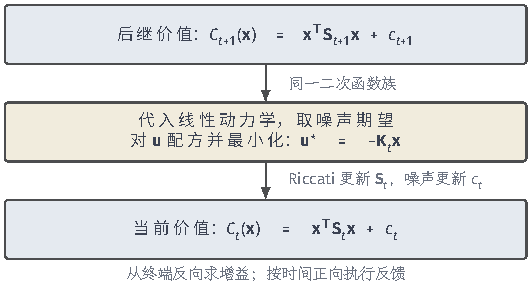
\includegraphics[width=89.958mm]{figures/10-reinforcement-learning/01-problems-and-solving/tikz/rl-planning-lqr-closure.pdf}
 \caption{有限时域LQR的封闭关系。给定线性动力学、二次成本与独立零均值加性噪声，最小化一步成本后仍得到二次价值加常数；增益由反向递推得到，控制按正向时间执行。}
 \label{fig:rl-planning-lqr-closure}
\end{figure}

有限时域封闭还不能保证时域趋于无穷后成本有限。对无噪声、无折扣的无限总成本，标准结果另要求$(\bm A,\bm B)$可稳定、$(\bm Q^{1/2},\bm A)$可检测，并保留$\bm Q\succeq0$、$\bm R\succ0$。可稳定意味着存在反馈，使闭环$\bm A-\bm B\bm K$的特征值落在单位圆内。可检测条件考察成本所衡量的量$\bm Q^{1/2}\bm x$：沿无输入状态动力学始终不能由这个量辨出的状态模式，必须自行衰减，其特征值严格落在单位圆内。这里需要考察模式随时间的演化，不是只检查某个时刻的状态是否满足$\bm Q^{1/2}\bm x=0$；所用的量也不是传感器观测，不能把这项成本条件替换成观测核的性质。在这些条件下，零终端成本的递推随时域延长，收敛到唯一半正定稳定化解$\bm S$。它满足将式~\eqref{eq:rl-planning-riccati}~中的$\bm S_t,\bm S_{t+1}$都替换成$\bm S$所得的代数Riccati方程。

这个无限时域结论还要求稳定化解，而不是任意代数方程解。持续非零噪声通常会使无折扣无限总成本发散，需要改用平均成本等准则；有限时域的常数项可以求出，并不代表无限累加仍有限。

% Outline: 2.3.2
\subsection{价值方程的可线性化结构}
\label{sec:rl-planning-kl-control}

LQR通过保留二次价值族减少了未知量，但每一步仍要做二次函数最小化和矩阵求逆。另一类结构走的是不同的简化路线：它不去限制价值的函数形式，而是限制“能选择哪些后继分布、偏离自然规律要付多少代价”，从而让原本含优化的价值方程可以通过一次换元变成线性方程。考虑这样一种控制视角：直接把下一步状态的概率分布当作可选择的对象；系统在不加干预时本来有一个自然转移，干预越强、分布偏离自然转移越多，费用就越高。\term{KL控制}用KL散度来计量这种偏离。要特别注意，它允许优化的是一族受支持约束的后继分布，而不是普通MDP里事先给定的那几个离散动作。

在普通MDP中，执行动作$a$只能得到接口规定的$T(\cdot\mid s,a)$；即使随机化动作，得到的也只是这些给定分布的凸组合，无法任意调配各后继的概率。KL控制的特殊设定则把“在自然规律已有的可能后继中重新分配概率”本身当作可选控制，并对偏离收费。因此两种接口即便支持的后继集合相同，也不代表物理执行器真能实现任意的概率重分配；使用下面的换元技巧前，必须先确认任务确实赋予了这种控制权限和对应的费用规则。

两个有限分布$p,q$之间的KL散度是按$p$平均的对数概率比：
\[
 D_{\mathrm{KL}}(p\Vert q)=\sum_{i:p_i>0}p_i\log\frac{p_i}{q_i}.
\]
$p_i=0$的项取0；若$p_i>0$而$q_i=0$，值为正无穷。对数取自然底。该量非负，且仅在$p=q$时为0，一般并不对称。只要将待优化成本改写成“一个不随候选改变的常数加非负KL项”，就能验证候选的全局最优性。这些性质以及收益与KL偏离权衡的指数倾斜结论，可参考\BookChapterRef{chap:information-theory-and-statistical-geometry}{卷2《数学准备：概率、因果与决策》的“概率分布的分析与优化”章}。

\begin{definition}[有限时域KL控制]
 \label{def:rl-planning-kl-control}
 给定非空有限状态集$S$、整数时域$H\geq1$、被动转移概率核$T_0(s'\mid s)$、有限实值成本$c_t:S\to\mathbb R$（$0\leq t<H$）和$g:S\to\mathbb R$，以及$\lambda>0$。在状态$s$可选择概率分布$u(\cdot\mid s)$，要求
 $T_0(s'\mid s)=0$时$u(s'\mid s)=0$。单步期望成本为
 \[
 c_t(s)+\lambda D_{\mathrm{KL}}(u(\cdot\mid s)\Vert T_0(\cdot\mid s)).
 \]
 目标是在所有允许的历史依赖分布控制中，最小化从$t$到$H-1$的上述成本之和加$g(s_H)$的期望，不折扣。最小剩余成本记为$V_t^{\mathrm c}(s)$，终端条件为$V_H^{\mathrm c}=g$；对应的奖励价值为$-V_t^{\mathrm c}$。
\end{definition}

被动转移$T_0$表示不施加这种分布控制时的自然规律。支持约束使控制只能重新分配自然规律已有的可能后继，不能以有限费用创造原本概率为零的转移。对支持内概率采用$0\log0=0$约定；严格正的$\lambda$保证偏离确实增加成本，控制必须权衡这项费用与未来成本。

给定下一时刻的最小成本$V_{t+1}^{\mathrm c}$，当前要在允许的概率分布$u$中，最小化KL费用加后继成本期望。我们先用被动概率和后继成本构造一个候选：令
$Z_t(s)=\sum_{s'}T_0(s'\mid s)\exp(-V_{t+1}^{\mathrm c}(s')/\lambda)>0$作为归一化系数，并取
\[
 u_t^*(s'\mid s)=
 \frac{T_0(s'\mid s)\exp(-V_{t+1}^{\mathrm c}(s')/\lambda)}{Z_t(s)}.
\]
有限状态、有限成本及$\lambda>0$保证$Z_t(s)>0$，候选$u_t^*$是合法概率分布，且与$T_0$有相同支持。有限分布的指数倾斜关系在这个支持集上给出：任意允许分布$u$的待优化成本满足
\begin{equation}
 \begin{aligned}
 &\lambda D_{\mathrm{KL}}(u\Vert T_0)
       +\sum_{s'}u(s'\mid s)V_{t+1}^{\mathrm c}(s')\\
 &\qquad=\lambda D_{\mathrm{KL}}(u\Vert u_t^*)-\lambda\log Z_t(s).
 \end{aligned}
 \label{eq:rl-planning-kl-completion}
\end{equation}
右侧第二项不随$u$改变，第一项非负且在$u=u_t^*$时为0。因此$u_t^*$在整个允许分布集合上达到最小值，不只满足一阶必要条件。加回当前状态成本，得到
\[
 V_t^{\mathrm c}(s)=c_t(s)-\lambda\log Z_t(s).
\]
这个最小值替代了原来的分布优化。$u_t^*$给低成本后继更大的指数权重，再由$T_0$和$Z_t$保持支持与归一化；指数中的负号来自成本越小越优，不能原样解释为奖励最大化中的偏好。

上式仍含对数，但我们可以改求成本的指数变换，而不直接求成本。令$z_t(s)=\exp(-V_t^{\mathrm c}(s)/\lambda)$，对等式两侧取相应指数，便有
\begin{equation}
 z_t(s)=\exp(-c_t(s)/\lambda)\sum_{s'}T_0(s'\mid s)z_{t+1}(s'),
 \qquad z_H(s)=\exp(-g(s)/\lambda).
 \label{eq:rl-planning-kl-linear}
\end{equation}
后继未知量$z_{t+1}$现在只出现在加权和中，所以这是线性反向递推。由终端值算出$z$后，再用
$u_t^*(s'\mid s)=T_0(s'\mid s)z_{t+1}(s')/\sum_xT_0(x\mid s)z_{t+1}(x)$
恢复最优转移，若需成本则用$V_t^{\mathrm c}=-\lambda\log z_t$还原。控制限制、指数变换和不同时间目标的关系可参见Todorov的原始工作\scite{rl2-todorov2006-linear}

用一个只剩一步的教学模型检查这种权衡。被动转移以相等概率到达两处，终端成本分别为0和$\lambda\log3$，当前状态成本为0。两处$z_H$为1和$1/3$，所以$Z=2/3$，最优受控概率为$(3/4,1/4)$，最小成本为$\lambda\log(3/2)$。若全部转向第一处，终端成本虽为0，偏离被动分布的费用却为$\lambda\log2$，总成本更高。因此最优分布仍给第二个后继保留概率。

线性化依赖刚才的控制费用和时间目标。表~\ref{tab:rl-planning-kl-regimes}~对照有限时域、终止型和平均成本中的边界条件。一般折扣成本方程含$\gamma V(s')$，同样换元得到$z(s)=e^{-c(s)/\lambda}\sum_{s'}T_0(s'\mid s)z(s')^\gamma$，通常仍然非线性。即使方程已经线性，也未必减少未知量个数：表格表示仍需保存每个状态的$z(s)$。

终止型总成本把固定时刻的终端边界改成首次到达终点集$B$时终止，并在到达状态支付给定成本$g_B$。这一行采用不随时间变化的状态成本$c(s)$，令$N=S\setminus B$为非终点集合。将被动核$T_0$按这两个集合分块，$\bm T_{NN}$收集从$N$到$N$的概率，$\bm T_{NB}$收集从$N$到$B$的概率，行均对应出发状态。对角矩阵$\bm G_N=\operatorname{diag}_{s\in N}(e^{-c(s)/\lambda})$给出非终点的成本因子，边值$\bm z_B=e^{-\bm g_B/\lambda}$按坐标取指数，因而方程中只剩$\bm z_N$未知。这是按状态集合分块，不是有限时域递推中的时间下标；表中的谱半径条件保证这组线性方程唯一可解，有限最优总成本还须另核终止问题的适定条件。

\begin{table*}[htbp]
 \centering
 \small
 \begin{tabularx}{\linewidth}{@{}l>{\raggedright\arraybackslash}X>{\raggedright\arraybackslash}X@{}}
  \toprule
  目标 & 换元后的关系 & 所需边界或附加条件\\
  \midrule
  有限时域 & $\bm z_t=\bm G_t\bm T_0\bm z_{t+1}$ & $\bm G_t=\operatorname{diag}(e^{-c_t/\lambda})$，终端$\bm z_H=e^{-\bm g/\lambda}$\\
  终止型总成本 & $\bm z_N=\bm G_N(\bm T_{NN}\bm z_N+\bm T_{NB}\bm z_B)$ & 固定终点集$B$的边值；如$\bm G_N\bm T_{NN}$的谱半径小于1，线性方程唯一可解\\
  平均成本 & $e^{-\bar c/\lambda}\bm z=\bm G\bm T_0\bm z$ & 有限不可约被动链、有限成本给正的Perron特征向量；只确定尺度，非周期性影响幂迭代\\
  一般折扣成本 & $\bm z=\bm G\bm T_0\bm z^\gamma$ & 幂按坐标作用；不再是线性方程\\
  \bottomrule
 \end{tabularx}
 \caption{KL控制的三类线性形式及折扣边界。终止型的$N$表示非终点集合，不是时间；平均成本的$\bar c$是每步最优平均成本。}
 \label{tab:rl-planning-kl-regimes}
\end{table*}

表中的平均成本关系来自$\bar c+V^{\mathrm c}(s)=c(s)-\lambda\log\sum_{s'}T_0(s'\mid s)e^{-V^{\mathrm c}(s')/\lambda}$的指数变换。此时$V^{\mathrm c}$是扣除平均增长后的差分成本，换元所得$z$只确定到尺度。不可约非负矩阵的Perron理论保证所需正特征向量；沿轨迹累加成本等式，再除以时长，有界差分成本的首尾项消失，从而验证平均成本最优性。这条证明使用特征值与平均成本关系，不是折扣压缩论证。

% Outline: 2.3.3
\subsection{最优策略的单调与阈值结构}
\label{sec:rl-planning-monotone}

在库存这类问题中，状态（库存数量）和动作（订货多少）本身都是可以排序的。如果每个库存水平都单独与所有动作逐一比较，就忽略了最优选择可能天然带有顺序规律。不过在使用顺序结构前，必须先说清动作究竟代表什么：当库存增加时，“订货量”可能下降，但“订货之后的总库存”却可能上升，两者的单调方向相反。\term{单调策略}指状态沿一个方向增大时，所选动作也始终沿某个固定方向变化；对只有两个动作的情形，这种规则往往只由一个切换点决定，称为\term{阈值策略}。库存中的\term{基库存策略}以$x$表示订货前的净库存，把订后库存设为$\max\{x,S_t\}$，订货量为$(S_t-x)_+$；其中$(z)_+=\max(z,0)$表示正部，所以库存一旦达到水平$S_t$就不再订货。这类规则把要描述的选择压缩成少数几个阈值或水平，但$S_t$具体取多少仍须根据模型和目标求出来。

怎样判断这种顺序关系是否真的成立？关键在于比较“选大动作比选小动作多花多少成本”如何随状态变化。如果状态越大，大动作相对小动作反而越便宜，那么最优选择就应当随状态增大而单调地偏向大动作。把当前成本与后继成本期望合起来记作一步目标$f(s,a)$，称它具有\term{递减差分}，若对$s_2\geq s_1$、$a_2\geq a_1$，
\begin{equation}
 f(s_2,a_2)-f(s_2,a_1)
 \leq f(s_1,a_2)-f(s_1,a_1).
 \label{eq:rl-planning-decreasing-differences}
\end{equation}
这个条件比较的是两动作成本之差，而不是要求每个动作的绝对成本下降。以下定理在共同的有限全序动作集中最小化$f$；遇到并列最小值时，统一选最大的动作，才能得到所述单调选择。更一般的格上比较静态结果见Topkis\scite{rl2-topkis1978-lattice}

\begin{theorem}[递减差分给出单调最优动作]
 \label{thm:rl-planning-monotone}
 设$(S,\leq)$为全序状态集，所有状态共享同一个非空有限全序动作集$\mathsf A$，$f:S\times\mathsf A\to\mathbb R$为一步成本目标。若对任意$s_2\geq s_1$、$a_2\geq a_1$都有$f(s_2,a_2)-f(s_2,a_1)\leq f(s_1,a_2)-f(s_1,a_1)$，则选取最大的最小化动作
 $a^*(s)=\max\arg\min_a f(s,a)$得到随$s$单调不减的策略。
\end{theorem}
\begin{proof}
 取$s_2\geq s_1$，记$a_1=a^*(s_1)$、$a_2=a^*(s_2)$。反设$a_2<a_1$。最优性给出
 $f(s_1,a_1)-f(s_1,a_2)\leq0$与
 $f(s_2,a_1)-f(s_2,a_2)\geq0$。递减差分又给出
 \[
 0\leq f(s_2,a_1)-f(s_2,a_2)
 \leq f(s_1,a_1)-f(s_1,a_2)\leq0.
 \]
 所有不等式只能取等号，故$a_1$也是$s_2$处的最小化动作。但$a_1>a_2$，与$a_2$是最大的最小化动作矛盾。因此$a_2\geq a_1$。
\end{proof}

将定理用于多步决策，还必须证明后继成本加入后，差分条件仍保持。考虑一个可逐步验证的排队模型：状态$x\in\{0,\ldots,B\}$表示有容量上限的队长，动作$a=0$保留队列，$a=1$立即清空。保留支付非负且随$x$不减的等待成本$h(x)$，清空支付固定成本$K>0$。随后产生与状态动作独立、分布已知的非负到达$W_t$，容量外到达丢弃且不另收费。两动作的后继分别为
$\min(x+W_t,B)$和$\min(W_t,B)$。取有限时域、无折扣、终端成本0。

若$C_{t+1}$单调不减，则
\[
 \begin{aligned}
 f_t(x,0)&=h(x)+\mathbb E C_{t+1}(\min(x+W_t,B)),\\
 f_t(x,1)&=K+\mathbb E C_{t+1}(\min(W_t,B)).
 \end{aligned}
 \]
保留目标随$x$不减，清空目标不随$x$变化，取两者最小值得到的$C_t$仍随$x$不减。从$C_H=0$反向归纳，这项性质逐步保持。与此同时，清空相对保留的成本差$f_t(x,1)-f_t(x,0)$随$x$不增，满足递减差分。因此在上述模型中，可以按阈值选择清空。若清空费用依赖队长、丢包另有复杂成本，或到达规律随服务动作变化，就必须重新验证每一步目标，不能只凭“排队模型”沿用阈值结论。

为求出阈值而不只说明其存在，取教学参数$B=5$、$h(x)=x$、$K=2.5$、$W_t=1$、$H=2$。最后一步最小成本为$C_1(x)=\min(x,2.5)$。在$t=0$，清空目标恒为$2.5+C_1(1)=3.5$，保留目标为$x+C_1(\min(x+1,5))$；后者在$x=0,1,2$分别为1、3、4.5，且继续随$x$不减。因此从$x=2$起清空更便宜，阈值为2，见图~\ref{fig:rl-planning-threshold}。

\begin{figure}[htbp]
 \centering
 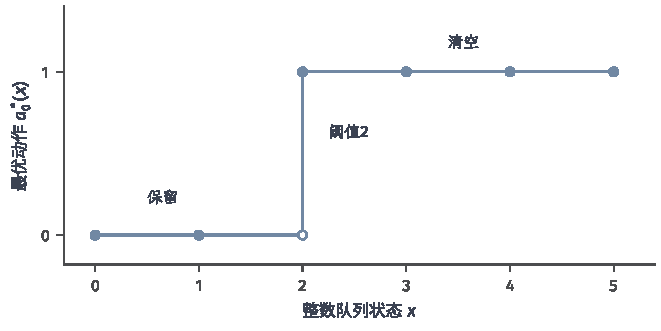
\includegraphics[width=112.000mm]{figures/10-reinforcement-learning/01-problems-and-solving/matplotlib/rl-planning-threshold.pdf}
 \caption{上述两步排队教学模型在$t=0$的最优动作。横轴是整数队长，纵轴0表示保留、1表示清空；连接线只帮助阅读阶梯形状，不表示连续状态模型。阈值2由列出的Bellman目标计算。}
 \label{fig:rl-planning-threshold}
\end{figure}

回到库存时，订后库存$y$受$y\geq x$约束，各状态的允许动作不同，不能直接套用共同动作集的定理。采用有限时域、无折扣的经典教学模型：净库存$x,y$取实数，负值表示结转的欠货；订货立即到达，无容量上限，也不允许通过负订货量处置库存。各期非负需求$D_t$分布已知、独立于过去和订货选择，需求后净库存为$y-D_t$。没有固定订货费，单位费$c\geq0$；以有限凸函数$\ell_t(z)$表示需求后净库存$z$的持有和缺货成本，以有限凸函数$C_H$表示终端成本。一步目标于是为
\[
 \begin{aligned}
 C_t(x)&=\min_{y\geq x}\{c(y-x)+
       \mathbb E[\ell_t(y-D_t)+C_{t+1}(y-D_t)]\}\\
       &=-cx+\min_{y\geq x}G_t(y),\\
 G_t(y)&=cy+\mathbb E[\ell_t(y-D_t)+C_{t+1}(y-D_t)].
 \end{aligned}
\]
还要求所列期望在每个实数$y$处有限，并且每期$G_t$在\emph{整个实数域}有有限的全局最小化点$S_t$；例如$G_t(y)\to+\infty$当$|y|\to\infty$，就是保证最小点存在的充分条件。仅要求每个$y\geq x$的受限问题能取到最小值并不够：若需求、持有和缺货成本及终端成本全为0而$c>0$，则$G_t(y)=cy$在每个受限域都于$x$取最小，却没有全域有限最小点。

若$C_{t+1}$凸，平移后的$\ell_t(y-D_t)+C_{t+1}(y-D_t)$对$y$仍凸，取期望保持凸性，再加线性项$cy$，得到凸的$G_t$。$-cx+G_t(y)$对$(x,y)$联合凸，约束$y\geq x$也为凸集合：两状态与各自最优订后库存的凸组合仍可行，把它代入目标便得到$C_t$的凸性不等式。因此从$C_H$反向归纳，凸性逐期保持。任取上述全局最小点$S_t$，当$x\leq S_t$时它可行且最优；当$x>S_t$时，凸函数在$S_t$右侧单调不减，受限最小值于$x$取到。故可选$y^*=\max(x,S_t)$，并非要求最优动作唯一。

例如最后一期取确定需求$D_{H-1}=2$、$c=1$、$\ell_{H-1}(z)=(z)_++3(-z)_+$、$C_H=0$，则$G_{H-1}(y)$在$y\leq2$时为$6-2y$，在$y\geq2$时为$2y-2$，从而$S_{H-1}=2$。订前库存1时订1，库存3时不订；订后库存随$x$不减，订货量随$x$不增。加入固定订货费、容量限制等条件后，目标或可行域改变，策略形状须重新推导。

% Outline: 2.3.4
\subsection{整体价值与策略的可分离结构}
\label{sec:rl-planning-separable}

当系统由若干彼此独立的设备组成时，联合状态是各设备状态的笛卡尔积，规模会随设备数急剧膨胀。我们很自然地希望分别求出每个子设备的局部价值、再相加，而不去枚举全部联合状态。但能否这样做，不只取决于各设备是否独立转移、奖励是否可加，还取决于动作选择是否也能各自独立进行：如果几台设备共享同一个操作者、每一步只能操作其中一台，就无法在同一时刻同时选取各自的最优动作。下面先给出直接分解成立所需的条件，再用反例说明共享资源会破坏其中的哪一步。

\begin{theorem}[独立子过程的可分离性]
 \label{thm:rl-planning-separable}
 设$m\geq1$个子过程具有有限状态集$S_i$、非空有限动作集$\mathsf A_i(s_i)$、转移核$T_i$及有界奖励$R_i$，共同折扣因子为$0\leq\gamma<1$。联合状态为$s=(s_1,\ldots,s_m)\in\prod_i S_i$，合法联合动作集是$\mathsf A(s)=\prod_i\mathsf A_i(s_i)$，且
 \[
 T(s'\mid s,a)=\prod_iT_i(s_i'\mid s_i,a_i),\qquad
 R(s,a)=\sum_iR_i(s_i,a_i).
 \]
 在有限状态动作的折扣问题中，$V^*(s)=\sum_iV_i^*(s_i)$，且各子过程的最优动作可分别选择。有限时域中，若各时刻仍满足上述乘积转移与可加奖励，终端价值也可加，则相同的价值分解及逐分量动作选择按时刻成立。
\end{theorem}
\begin{proof}
 对任意可加函数$v(s)=\sum_i v_i(s_i)$，利用转移的乘积形式并对其他坐标求和，
 \[
 \sum_{s'}T(s'\mid s,a)v(s')
 =\sum_i\sum_{s_i'}T_i(s_i'\mid s_i,a_i)v_i(s_i').
 \]
 因为每个$a_i$可以独立地在$\mathsf A_i(s_i)$中选择，
 \[
 \begin{aligned}
 (\mathcal B^*v)(s)
 &=\max_{a_1,\ldots,a_m}\sum_i
   \left[R_i(s_i,a_i)+\gamma\sum_{s_i'}T_i(s_i'\mid s_i,a_i)v_i(s_i')\right]\\
 &=\sum_i(\mathcal B_i^*v_i)(s_i).
 \end{aligned}
 \]
 最后一个等式的两个方向分别来自“任意动作的和不超过各自最大值之和”和“同时选择每个最大化动作便达到该和”。有限时域由可加终端值反向归纳，且逐层的独立最大化恢复策略。折扣情形取各子过程不动点$v_i=V_i^*$，其和成为联合$\mathcal B^*$的不动点；唯一性给出联合最优价值，独立最大化动作构成联合最优策略。
\end{proof}

图~\ref{fig:rl-planning-factorization}~上部的两个子网格各自接收动作，允许同时执行局部最大化选择；若改为每步最多激活一个，证明中把联合最大值拆成各自最大值之和的等式就不再成立。一个最小反例是两个单状态设备：激活每步得1，空闲得0，状态恒定。在笛卡尔积动作下可同时激活，联合价值为$2/(1-\gamma)$；互斥激活后只能得到$1/(1-\gamma)$。因此独立转移不足以保证局部最优价值相加。

\begin{figure}[htbp]
 \centering
 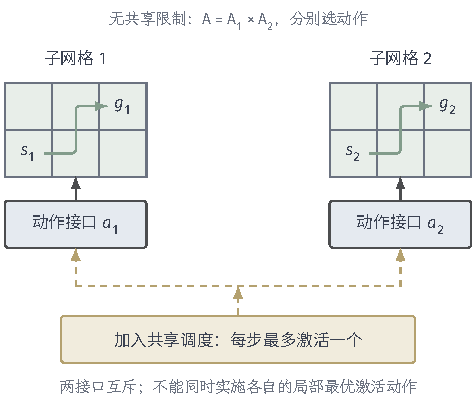
\includegraphics[width=80.617mm]{figures/10-reinforcement-learning/01-problems-and-solving/tikz/rl-planning-factorization.pdf}
 \caption{可分解的动力学不等于可分解的决策。上部两个子网格分别接收$a_1,a_2$；下部共享调度选择只能激活一个接口，使联合动作集不再是原局部动作集的笛卡尔积。}
 \label{fig:rl-planning-factorization}
\end{figure}

共享激活虽然破坏了直接相加，但若结构足够特殊，仍可能找到避免联合枚举的办法。\term{经典冻结型Markov老虎机}（rested Markov bandit）把每个独立设备看成一只“臂”：只有当前被激活的那只臂才会发生状态转移并产生奖励，其余臂的状态一律冻结、奖励为0；每步恰好激活一只臂，且切换不收费。若每只臂只有一个不变状态，问题就简化为每步从若干奖励来源中选一个；现在每只臂内部还会随激活演化，所以当前选择也会影响以后可得的奖励。在有限状态、已知转移、有界非负奖励、共同$0<\gamma<1$及无限时域目标下，Gittins指数定理给出一个结构性结论：可以给每只臂在当前状态下单独算出一个数（指数），然后每一步只需激活当前指数最大的那只臂，无须维护联合状态上的价值表。奖励规律未知、必须边试验边估计的老虎机探索，则由第~\ref{chap:rl-learning}~章讨论。

这个数要衡量的不是“下一步奖励”，而是“持续使用这只臂一段时间，平均每单位折扣时间能换来多少收益”，从而允许为了将来的高收益先承受眼前的低收益。对臂$i$当前状态$x$，我们允许根据已看到的局部历史决定何时停止，且至少激活一次；在所有这样的停止规则中，取期望累计奖励与期望累计折扣时间之比的上确界：
\begin{equation}
 \nu_i(x)=\sup_{\tau\geq1}
 \frac{\mathbb E_x\sum_{t=0}^{\tau-1}\gamma^t R_i(X_t)}
      {\mathbb E_x\sum_{t=0}^{\tau-1}\gamma^t},
 \label{eq:rl-planning-gittins}
\end{equation}
其中$X_t$是持续激活该臂时的局部状态过程，$\tau$是由该臂已见历史决定的停止时刻，$\tau\geq1$保证分母为正。固定一份停止规则并反复运行时，先分别计算收益与折扣占用时间的期望，再将两者相除；这通常不同于先算每条轨迹的收益时间比再取平均。允许在看到不利局部状态后停止，正是它区别于当前一步奖励的地方。用上确界容纳所有允许的停止规则，不要求某个有限停止时刻必定取到它。也可以把候选指数$\lambda$当作每次激活的机会成本，考察净收益
$\sup_{\tau\geq1}\mathbb E_x\sum_{t<\tau}\gamma^t(R_i(X_t)-\lambda)$，
净收益由正转为非正的临界$\lambda$给出上述指数。全局最优性并非来自价值直接相加，而是利用未激活臂的冻结性，交换比较竞争臂的激活片段，证明按指数排序不损失回报。完整指数理论与局部计算方法见Gittins的原文\scite{rl2-gittins1979-index}

用一个两状态教学例观察指数为何不同于即时奖励。某臂从$x$开始，激活时奖励为0并确定转到$y$；在$y$激活时奖励为1，且状态保持$y$。未激活时两状态都冻结，奖励为0，取$\gamma=1/2$。若连续激活$k\geq1$次后停止，时间按该臂的激活次数计算，这条确定轨迹的收益与折扣占用时间之比为
\[
 \frac{\sum_{t=1}^{k-1}2^{-t}}{\sum_{t=0}^{k-1}2^{-t}}
 =\frac{2^{k-1}-1}{2^k-1}
 =\frac12-\frac{1}{2(2^k-1)}.
\]
激活一次的比率为0，激活两次为$1/3$，随$k$增加趋于$1/2$。由于状态演化确定，非随机停止规则在这条轨迹上就是选择停止次数；随机停止也不能超过这些比率的上确界，因为每条轨迹的收益都至多为其折扣占用时间的一半，分别取期望后该不等式仍成立。因此$\nu_i(x)=1/2$，虽然$x$的即时奖励为0。只允许有限停止时，没有某个有限$k$取到这一上确界；若允许永久激活，则得到同一数值。这个例子展示了继续激活的未来收益怎样进入指数，全局指数规则的最优性仍依赖前述冻结性等条件。

若未激活的臂也会演化，即restless情形，等待期间的状态会改变，刚才利用冻结性交换片段的依据就不再适用；任意有限截止日期或切换成本也不在此定理范围内。各臂内部仍可能具有封闭、可线性化或单调结构，但简化局部计算并不自动解决共享激活造成的全局耦合。

% Outline: 2.4
\section{有限预算下的当前状态规划}
\label{sec:rl-planning-local-search}

前面的精确方法都是在行动之前，就为整个状态空间算出价值或反馈律。但很多实时系统做不到这一点：导航机器人此刻就需要下一步动作，没有预算先把成千上万甚至无穷多个状态全部算完。于是出现另一条思路——只为“当前所在的这一个状态”向前展开可能发生的后果，据此立刻给出一个动作；等真正走到新状态后，再在那里重新展开一次。这称为局部搜索。它把计算时间集中花在当前决策上，代价是不保存覆盖全部状态的完整解，因此每次到达新状态往往都要重新搜索。

% Outline: 2.4.1
\subsection{有限预算下的近似规划问题}
\label{sec:rl-planning-local-budget}

设机器人已经位于某个网格状态，当前这次规划只需返回一个动作，也可以附带给出各候选动作的价值估计。评价这样一个规划器要同时看两件事：首动作的长期后果是否选得好，以及它是否赶在行动截止时间之前算出来、用了多少次模型查询、占用多少搜索内存。这里要特别区分两种预算：全状态方法可能先花较长时间离线预计算，但执行时只需查一次表；局部方法几乎不需要预计算、总查询量也可能更少，但单次搜索仍可能超时。因此比较二者时，预计算预算和行动时预算应分别记账。

图~\ref{fig:rl-planning-search-tree}~展示了一次局部搜索可以从四个方面控制规模：限制向前看的步数（深度）、限制每层展开的分支数（宽度）、在停止展开处补上对未来价值的估计（叶值）、以及根据已有结果决定下一次模拟走哪条路径（自适应分配）。它们裁剪的是同一棵树的不同部分，可以组合使用；后文将分别分析每种手段省下了什么计算、又留下了什么误差。

\begin{figure}[htbp]
 \centering
 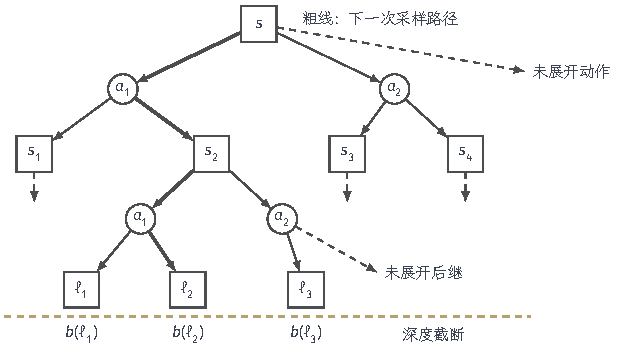
\includegraphics[width=105.138mm]{figures/10-reinforcement-learning/01-problems-and-solving/tikz/rl-planning-search-tree.pdf}
 \caption{局部搜索中的四种预算安排。方框是状态处的动作选择，圆点是选定动作后的随机后继选择；虚线边表示未展开的分支，底部虚线表示深度截断，叶子处的$b$为剩余价值估计。加粗路径表示下一次模拟的一个可能样本路径，不表示确定的环境转移。}
 \label{fig:rl-planning-search-tree}
\end{figure}

具体怎样展开，仍由模型接口决定：若模型直接给出非零概率的后继，就可以逐个列出并加权求精确和；若只有生成模型，一次查询只产生一个随机后继，就必须靠重复查询的均值来估计期望。无论哪种接口，都要严格区分树中的两类节点——哪些是规划器可以选择的动作，哪些是动作之后只能接受、无法挑选的随机结果。规划器能决定“查询哪个动作”，却不能在看到随机后继后专挑最有利的那个当作必然结果；即使采样完全正确，有限次模拟仍会带来统计误差。

% Outline: 2.4.2
\subsection{未来步数受限的搜索空间构造}
\label{sec:rl-planning-horizon-search}

一棵无限向前生长的搜索树在计算上不可行，最直接的裁剪是只看有限步：先精确计算当前状态$s$起$H$步内的奖励，至于第$H$步之后那部分尚未展开的未来，则用一个边界函数$b$给出估值补上。允许策略$\sigma$在这$H$步内根据实际到达的状态选择合法动作，以期望折扣回报最大为准，在这些策略中取上确界：
\begin{equation}
 U_H^b(s)=\sup_\sigma\mathbb E_\sigma\!\left[
 \sum_{t=0}^{H-1}\gamma^t r_t+\gamma^H b(s_H)
 \,\middle|\,s_0=s\right].
 \label{eq:rl-planning-lookahead}
\end{equation}
这里$b(s_H)$是到达搜索边界时对剩余回报的估计，它要乘$\gamma^H$，是因为这部分回报从第$H$步才开始计算，折算回当前时刻必须整体打$H$次折扣。式中的策略$\sigma$能够根据实际观察到的后继随时调整后续动作，因此我们优化的是一棵“看到结果再决定下一步”的反馈决策树，而不是一条事先定死、无法回应随机滑移的动作序列。在有限状态动作下，可以从$U_0^b=b$出发，逐层用$U_h^b=\mathcal B^*U_{h-1}^b$精确算出这棵树。特别要注意，取$b=0$只是在计算时忽略搜索范围之外的回报，相当于一种近似，并没有真的把任务改成在第$H$步终止——真实的终点奖励可能仍在更远处。

\term{滚动时域规划}（receding-horizon planning）的用法是：每次求出这棵有限树后只执行根部的第一个动作；待观察到实际新状态，再从那里重新规划同样长度的$H$步。这样能根据真实滑移不断修正后续选择，但“重新规划”本身并不会自动补回边界之外被忽略的价值。要判断有限前瞻究竟有多准，仍须控制边界估值的误差、以及它如何随层数向根部传播。

\begin{theorem}[有限前瞻的终端误差]
 \label{thm:rl-planning-terminal-error}
 设时间齐次MDP的状态动作有限、各动作集非空、奖励满足$|r_t|\leq R_{\max}<\infty$，且$0\leq\gamma<1$。给定整数$H\geq1$和终端函数$b,\tilde b:S\to\mathbb R$，$U_H^b$表示从当前状态起在所有合法反馈策略中最大化前$H$步折扣奖励加$\gamma^H b(s_H)$所得的价值。则
 \[
 \lVert U_H^b-U_H^{\tilde b}\rVert_\infty
 \leq\gamma^H\lVert b-\tilde b\rVert_\infty.
 \]
 特别地，若$\lVert b-V^*\rVert_\infty\leq\varepsilon$，
 则$\lVert U_H^b-V^*\rVert_\infty\leq\gamma^H\varepsilon$；
 零终端值满足
 $\lVert U_H^0-V^*\rVert_\infty\leq\gamma^H R_{\max}/(1-\gamma)$。
 固定同一策略序列、比较其两个终端估值时，同样成立。
\end{theorem}
\begin{proof}
 对任意同一策略序列，两个$H$步目标的前$H$步奖励相消，差只剩
 $\gamma^H\mathbb E[b(s_H)-\tilde b(s_H)]$，绝对值不超过
 $\gamma^H\lVert b-\tilde b\rVert_\infty$。对两个目标分别取上确界，利用
 $|\sup f-\sup g|\leq\sup|f-g|$，该界仍成立。也可逐层使用期望的非扩张性和最大化的非扩张性，每层再乘$\gamma$，得到同一结果。

 取$\tilde b=V^*$时，$\mathcal B^*V^*=V^*$保证$U_H^{V^*}=V^*$，即得第二条。又因$\lVert V^*\rVert_\infty\leq R_{\max}/(1-\gamma)$，令$b=0$得到零边值界。它也等于直接控制尾和
 $\sum_{t=H}^{\infty}\gamma^t|r_t|\leq\gamma^H R_{\max}/(1-\gamma)$所得的界。
\end{proof}

终端误差界控制的是$H$步前瞻值，还不是滚动执行策略的价值。若每次使用相同$H$、边界函数$b$及固定并列规则，精确根动作便定义一个平稳策略。计算根动作时，当前奖励后面接的是剩余$H-1$步的$U_{H-1}^b$，所以该策略对$U_{H-1}^b$贪心，不是对$U_H^b$贪心。由定理~\ref{thm:rl-planning-greedy-loss}，当$H\geq1$且$\lVert b-V^*\rVert_\infty\leq\varepsilon$时，其长期损失至多
$2\gamma^H\varepsilon/(1-\gamma)$。这才把前瞻精度与反复执行的性能联系起来。

\begin{example}[同一障碍下的短前瞻]
 \label{ex:rl-planning-detour}
 为隔离时域的影响，采用基准网格的坐标、障碍和终点，但将起点改为$(1,2)$，取消滑移，使合法动作确定执行；奖励和$\gamma=0.9$不变，所有搜索使用$b=0$。从起点向上绕过障碍，最短4步到终点；向下进入底部通道，至少6步到终点。

 长度$L$的确定到达路径的回报为
 $-0.04\sum_{t=0}^{L-2}0.9^t+0.9^{L-1}$。
 当$H=2$时，上、下动作的最优截断回报都为$-0.076$，按“下优先”的并列规则会选下。当$H=4$时，向上的分支已经看到终点，回报为$0.6206$；向下的分支仍只有四次步成本，回报为$-0.13756$。完整6步底部路线的回报为$0.426686$，也低于上方路线。
\end{example}

图~\ref{fig:rl-planning-detour}~让我们看到，短前瞻的并列来自两条分支都还没有计入终点收益。重复短规划未必解决这个问题：始终取$H=1$和“下、上、右、左”的并列次序，起点会向下，底部左格又向上，形成往返。若某个早期动作不可逆，后来即使延长搜索，也不能撤销已经付出的损失。

\begin{figure}[htbp]
 \centering
 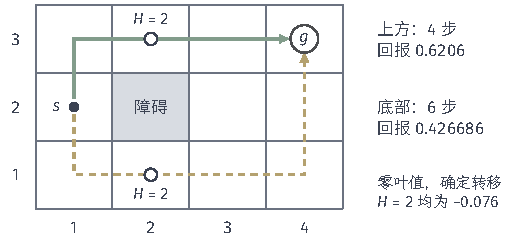
\includegraphics[width=86.847mm]{figures/10-reinforcement-learning/01-problems-and-solving/tikz/rl-planning-detour.pdf}
 \caption{确定性教学变体中的两条绕行路线。实线为4步上方路线，虚线为6步底部路线；标记$H=2$说明两个首动作在零叶值下都尚未看到终点。图中条件仅用于示例~\ref{ex:rl-planning-detour}，不替代基准随机网格。}
 \label{fig:rl-planning-detour}
\end{figure}

% Outline: 2.4.3
\subsection{未来分支受限的搜索空间构造}
\label{sec:rl-planning-sparse-search}

即使把深度限制为$H$，这棵树仍然可能太宽：每个状态都有若干候选动作，每个动作之后又有若干随机后继。裁剪宽度有两种性质完全不同的做法，必须分清：限制动作数是在删掉规划器本来可以选择的选项，可能因此漏掉真正最优的动作；限制随机后继数则不改变可选动作，只是用有限样本来近似“执行该动作后期望发生什么”。后者保留了动作选择本身，却引入了采样误差。

\term{稀疏采样}（sparse sampling）采取后一种做法：保留对有限动作的逐一枚举，但只为每个动作从生成模型独立抽取$m$个后继，再递归地计算这些样本上的未来价值，用样本均值近似随机后果的期望。取零叶值时，递归写为
\begin{equation}
 \begin{aligned}
 \widehat U_0(s)&=0,\\
 \widehat Q_h(s,a)&=\frac1m\sum_{j=1}^{m}
       \bigl[r_j+\gamma\widehat U_{h-1}^{(j)}(s'_j)\bigr],\\
 \widehat U_h(s)&=\max_{a\in\mathsf A(s)}\widehat Q_h(s,a).
 \end{aligned}
 \label{eq:rl-planning-sparse-sampling}
\end{equation}
其中$j$编号的是同一$(s,a)$下的样本$(r_j,s'_j)$，不是轨迹时刻；$\widehat U_{h-1}^{(j)}$来自第$j$棵递归子树，而非同一张表的第$j$轮更新。每棵子树继续使用新样本。若每处动作数至多为$A$，一层为$A$个动作各付出$m$次查询，并为每个样本建立子树，因此
$C_0=0$、$C_h\leq Am(1+C_{h-1})$，进而
$C_H\leq\sum_{\ell=1}^{H}(Am)^\ell$。计数不显含全状态数，却仍可能随深度迅速增长。

我们还要判断这些有限样本能否可靠选择根动作。若$R_{\max}=0$，奖励、零叶值递推的理想值和采样估计都恒为0，估计误差也恒为0，无须使用尾概率界。下面只在$V_{\max}>0$时分析波动。先保留理想子值$U_h^0$，只分析一次均值估计；有界奖励和折扣使
$r+\gamma U_{h-1}^0(s')\in[-V_{\max},V_{\max}]$。
对一个动作的$m$个独立样本，Hoeffding不等式给出：$m$个独立、同分布于$[-V_{\max},V_{\max}]$内的随机变量，其均值偏离期望超过$\eta>0$的概率至多$2\exp[-m\eta^2/(2V_{\max}^2)]$。该界用于为每个模型查询均值分配允许的失败概率；独立有界随机量的集中条件可参考\BookChapterRef{chap:random-sequences-and-processes}{卷2《数学准备：概率、因果与决策》的“随机序列与随机过程”章}。
树中需要估计的动作均值至多有
$M=A\sum_{\ell=0}^{H-1}(Am)^\ell$个。即使节点状态由祖先样本决定，在给定祖先后，该节点的新样本仍独立，且相同的概率界一致成立。因此联合失败概率至多
$2M\exp[-m\eta^2/(2V_{\max}^2)]$。

只控制根部的一次均值还不够，实际计算使用的是带误差的递归子值。为了分开抽样波动与子树误差，对剩余$h$层的一个节点和动作，先用同一批$(r_j,s'_j)$配合理想子值，构造辅助均值
\[
 \widetilde Q_h(s,a)=\frac1m\sum_{j=1}^{m}
       [r_j+\gamma U_{h-1}^0(s'_j)].
\]
它的期望是理想动作价值
$Q_h^0(s,a)=R(s,a)+\gamma\sum_{s'}T(s'\mid s,a)U_{h-1}^0(s')$。
前面的集中界控制的是$|\widetilde Q_h-Q_h^0|$；实际估计$\widehat Q_h$与辅助均值的差，则只来自同一批后继处使用了不同的子值。在树内所有辅助均值误差均不超过$\eta$的联合事件上，令$e_{h-1}$同时界住相关子树的估值误差，三角不等式给出
\[
 \begin{aligned}
 |\widehat Q_h(s,a)-Q_h^0(s,a)|
 &\leq |\widehat Q_h(s,a)-\widetilde Q_h(s,a)|
       +|\widetilde Q_h(s,a)-Q_h^0(s,a)|\\
 &\leq\gamma e_{h-1}+\eta.
 \end{aligned}
\]
对合法动作取最大值不会放大这个统一误差上界，因而剩余$h$层的状态估值误差满足
$e_h\leq\eta+\gamma e_{h-1}$、$e_0=0$，从而
$e_H\leq\eta(1-\gamma^H)/(1-\gamma)$。
根部各动作值的误差也有同样上界；按估计值选动作相对理想$H$步最优首动作的损失不超过$2e_H$。再单独加上截断误差，才能联系无限时域目标。选择$m$使上述失败概率不超过指定$\alpha$便得到一条充分保证；$M$也依赖$m$，故这是需满足的隐式条件，而不是忽略树大小的一次均值估计。

上述保证依赖独立生成查询、有限动作、奖励界，以及对整棵有限树的误差联合控制，不能只靠某个节点的均值准确。Kearns等给出了更系统的分析：当前状态规划可以不显含全状态数，但精度要求和有效时域，即折扣尾部尚不能忽略的步数，仍可能使查询代价很高\scite{rl2-kearns2002-sparse}

固定$m$会为各节点预先分配相同宽度，也可以把展开数量与实际访问次数联系起来。\term{渐进加宽}（progressive widening）在节点访问少时保留少量候选，随着访问增加再加入动作或后继。图~\ref{fig:rl-planning-widening}~对照同一个父节点的预设宽度与增长宽度；这改变的是展开预算，不会自动提供最优性保证。

\begin{figure}[htbp]
 \centering
 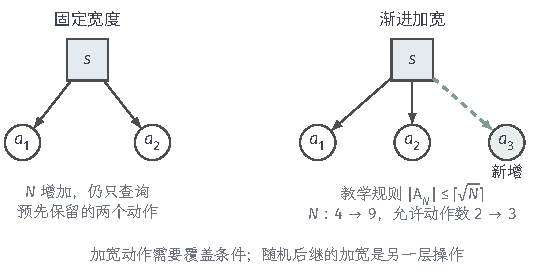
\includegraphics[width=90.318mm]{figures/10-reinforcement-learning/01-problems-and-solving/tikz/rl-planning-widening.pdf}
 \caption{固定分支与渐进加宽。左侧预先只保留两个动作；右侧在节点访问次数$N$增加后加入第三个动作，虚线标记本次新增边。若加宽的是随机后继而非动作，应在每个动作节点内部另行实施，不能混为同一次动作筛选。}
 \label{fig:rl-planning-widening}
\end{figure}

例如以节点访问次数$N$限制动作数为$\lceil cN^\beta\rceil$，其中$c>0$、$0<\beta<1$，使候选数增长慢于访问数，给已有候选留下重复评估的预算。在连续动作中，还要说明怎样提出新动作、最优动作附近能否被采到，以及邻近动作价值是否足够接近。若加宽随机后继，保留与重采样也必须保持正确的转移概率含义。这些条件缺失时，树变大仍不构成最优性证书。

% Outline: 2.4.4
\subsection{搜索空间外的未来价值评估}
\label{sec:rl-planning-leaf-value}

当搜索在一个尚未到达终点的格子停止展开时，后续奖励仍然真实存在、仍属于任务目标，只是我们没有继续把树画下去。因此需要对“这部分未展开的回报”给出一个估值，作为式~\eqref{eq:rl-planning-lookahead}~中的边界函数$b$，这就是\term{边界价值评估}。常见的有四种来源，它们补在搜索树的同一个边界位置，但所评价的后续行为和代价各不相同：直接取零等于忽略它；启发式依据问题知识估一个数；基础策略的\term{rollout}从叶子出发按某条既定规则继续模拟、再累计所得奖励；近似价值函数则用一组共享参数直接对叶子求值。

固定示例~\ref{ex:rl-planning-detour}~中的两处叶子$p=(2,3)$和$q=(3,2)$，它们在确定性变体中都恰好距终点两步。最佳剩余回报同为$-0.04+0.9=0.86$。表~\ref{tab:rl-planning-leaf-values}~在这同一对叶子上比较四种接口；所有数字均为教学设定。

\begin{table*}[htbp]
 \centering
 \small
 \begin{tabularx}{\linewidth}{@{}lcc>{\raggedright\arraybackslash}X>{\raggedright\arraybackslash}X@{}}
  \toprule
  边界规则 & $b(p)$ & $b(q)$ & 额外调用 & 偏差与方差\\
  \midrule
  零值 & $0$ & $0$ & 0 & 忽略真实剩余回报，无采样方差\\
  距离启发式 & $0.9$ & $0.9$ & 已知距离时为0 & 只计终点折扣、漏计步成本；此例高估$0.04$\\
  基础策略rollout & $0.86$ & $0.6206$ & 每条轨迹分别2、4次 & 基础策略在$q$多走两步；确定性模型中方差为0\\
  近似价值函数 & $0.80$ & $0.82$ & 求值时为0 & 给定的教学预测；相对$V^*$误差分别$-0.06,-0.04$\\
  \bottomrule
 \end{tabularx}
 \caption{固定叶子的四类评估。rollout基础策略在$p$走$p\to(3,3)\to g$，在$q$走$q\to(3,1)\to(4,1)\to(4,2)\to g$；预测数值不是训练实验结果，计算或训练这些预测的前期代价未计入在线调用。}
 \label{tab:rl-planning-leaf-values}
\end{table*}

表中的rollout差别来自基础策略的路线，而不是采样波动。模型随机时，rollout估计的仍是所选基础策略$\pi_{\mathrm b}$的$V^{\pi_{\mathrm b}}$，不自动是$V^*$。平均$N$条独立完整回报可减小采样方差，却不会改变基础策略的次优性。若只模拟$L$步再置零，还会相对$V^{\pi_{\mathrm b}}$留下至多$\gamma^L V_{\max}$的尾误差。折扣任务可能没有自然终止，因此完整rollout也未必能在有限次调用内结束。

定理~\ref{thm:rl-planning-terminal-error}~给出了资源取舍：减小边界误差或增加深度，都能降低传到根部的误差上界。加深会扩大搜索树，改进叶值则可能复用之前算出的价值。不过，网络在其他区域预测准确，不能代替当前搜索叶子上的误差控制。这里先讨论如何使用叶值；跨状态表示和评价近似价值的方法由下一节展开。

% Outline: 2.4.5
\subsection{搜索预算的自适应分配}
\label{sec:rl-planning-mcts}

如果在同一个根状态反复模拟，很快会出现一个资源分配问题：有些动作已经模拟很多次、证据较充分，有些动作几乎没试过、价值仍很不确定。若每次都对所有分支平均用力，往往不划算。\term{蒙特卡罗树搜索}（Monte Carlo tree search, MCTS）的思路是保存各节点的访问统计，用已有的模拟结果决定下一次该往哪条路径深入：一次模拟从根出发，沿已建成的树选择动作，遇到尚未充分展开的节点就扩展，再评估叶子的回报，最后把沿途奖励连同折扣后的叶值逐层回传、更新统计。整个过程中要分清两种选择：树内“走哪条分支继续模拟”由搜索规则决定，而动作之后到达哪个后继仍由模型随机采样，二者不能混为一谈。

这些统计量按搜索树节点分别保存。同一个环境状态可能由不同路径到达，也可能对应不同的剩余深度；它在树中的这些节点各有自己的访问次数和平均回报。下面的$N(s,a)$、$\bar Q(s,a)$用节点所处的环境状态$s$作简记，省略路径与剩余深度标记，不表示仅按环境状态共享统计。若另做节点合并，至少须保留剩余深度，并核对后续模型、合法动作与叶值规则是否相同；仅凭环境状态相同不足以合并这些统计量。

为了同时利用“已知回报较高的动作”和“还没怎么试过的动作”，在当前节点的每条动作边$(s,a)$上记录访问次数$N(s,a)$和从该边起算的平均折扣回报$\bar Q(s,a)$，并令$N(s)=\sum_aN(s,a)$。\term{UCT}（upper confidence bounds applied to trees）给每个动作打一个由两部分相加的分数，用它决定树内下一次模拟走哪条边；对已访问的合法动作，选择分数最大的一个：
\begin{equation}
 a\in\arg\max_a\left[
 \bar Q(s,a)+c\sqrt{\frac{\log N(s)}{N(s,a)}}\right],
 \label{eq:rl-planning-uct}
\end{equation}
第一项$\bar Q$是“利用”：偏向目前平均回报高的动作；第二项随$N(s,a)$增大而减小，是“探索”：访问得越少的动作，这项加分越大，越有机会补充证据。其中$c>0$要与回报的数值尺度相配；未访问过的动作先至少试一次，以免分母为零。要强调的是，这个分数只用于决定把查询预算投向哪里，第二项并不是环境真正给出的奖励。预算用尽、需要输出最终动作时，通常按访问次数或平均回报来选、不再加探索项，因此报告时必须写明最终采用的规则。

图~\ref{fig:rl-planning-mcts}~用一条教学记录展示分数、叶值和回传怎样共同改变预算。人为给定根状态$(1,1)$两条边的统计量：
$N(\text{右})=4,\bar Q(\text{右})=0.30$，
$N(\text{上})=1,\bar Q(\text{上})=0.20$，
取$c=0.20$。UCT分数分别约为$0.427$与$0.454$，因此下一次模拟先试“上”。假定本次没有滑移，到达$(1,2)$，当步奖励$-0.04$，叶估值$b=0.70$；回传值为
$g=-0.04+0.9\times0.70=0.59$。
这是假设的单次搜索记录，$0.70$不是该状态的真实最优价值。更新后
$N(\text{上})=2$，
$\bar Q(\text{上})=(1\times0.20+0.59)/2=0.395$。
此时两条分数约为$0.434$与$0.584$，下一次仍偏向“上”。一次乐观叶估值会改变后续预算，因此访问次数大并不自行证明估值正确。

\begin{figure}[htbp]
 \centering
 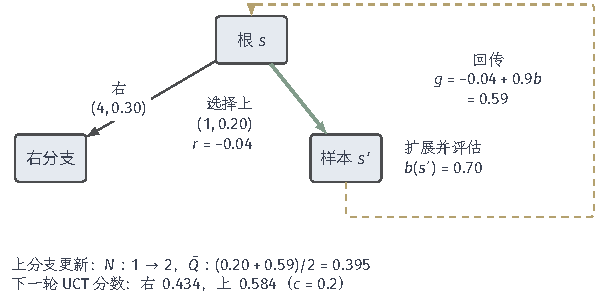
\includegraphics[width=101.388mm]{figures/10-reinforcement-learning/01-problems-and-solving/tikz/rl-planning-mcts.pdf}
 \caption{一次MCTS模拟及回传。边标签列出模拟前的$(N,\bar Q)$；本次选择“上”，扩展到样本后继，用$b=0.70$评估叶子，并回传$0.59$，得到更新后的$(2,0.395)$。箭头旁分别标明树内选择与统计量回传，数字为正文规定的教学记录。}
 \label{fig:rl-planning-mcts}
\end{figure}

若路径更深，先从叶值开始，用$g_t=r_t+\gamma g_{t+1}$逐层算回各边起点的回报，再更新对应边的统计量：
$N\leftarrow N+1$、
$\bar Q\leftarrow\bar Q+(g_t-\bar Q)/N$。
各边的奖励起算时刻和折扣次数不同，因此不能把根部累计回报原样写入所有深度。

UCT的探索项借鉴了老虎机的上置信界（upper confidence bound, UCB），即给证据不足的动作增加乐观估值。不过，树内下游搜索规则会不断改变，同一边以后模拟的回报分布未必与早期相同，不能直接套用固定分布老虎机的全部结论。原始UCT分析在有限动作、有界回报和有限深度等条件下沿树深归纳，处理这种变化；折扣问题还需加入截断误差。即使原设定下一致，也不代表任意先验、叶网络或连续加宽方案都有相同有限样本保证\scite{rl2-kocsis2006-uct}

在棋类中，合法走子和状态转移由规则给定，难点是无法穷举全部后续局面。AlphaZero把网络给出的动作先验和局面价值接入搜索：先验提示哪些动作先分配预算，价值估计尚未展开的未来，模型仍由已知规则提供。因此学习这些建议不等于学习环境动力学\scite{rl2-silver2018-alphazero}

具体地，AlphaZero使用带策略先验的PUCT式选择，按先验概率调整探索分配，其典型探索项与
$p(a\mid s)\sqrt{N(s)}/(1+N(s,a))$成正比，而非直接照抄式~\eqref{eq:rl-planning-uct}。表~\ref{tab:rl-planning-alphazero}~区分环境规则、动作先验、叶值与搜索统计的职责。

\begin{table*}[t]
 \centering
 \small
 \begin{tabularx}{\linewidth}{@{}l>{\raggedright\arraybackslash}X>{\raggedright\arraybackslash}X@{}}
  \toprule
  部件 & 无学习先验的基本搜索 & AlphaZero中的接口\\
  \midrule
  环境后果 & 用精确规则或模型样本展开 & 已知棋类规则，不以学习动力学为必要条件\\
  动作预算 & 根据均值和探索项分配 & 策略先验影响早期访问分配；先验错误可能浪费预算\\
  叶子价值 & 零值、启发式或rollout & 价值网络估计当前局面结果，仍有逼近误差\\
  搜索输出 & 根动作及其统计量 & 根访问分布提供动作选择依据，并作为策略训练目标\\
  训练反馈 & 可以完全没有训练阶段 & 自我对弈结果训练价值；对手策略与自我对弈训练记录的分布随策略变化\\
  \bottomrule
 \end{tabularx}
 \caption{已知模型搜索中规则、先验、叶值和搜索目标的不同作用。棋类回报与双方轮流行动的符号按当前玩家处理，不能直接套用单智能体网格的同向回报。}
 \label{tab:rl-planning-alphazero}
\end{table*}

已知规则、动作建议和叶值承担不同职责，搜索可以组合给定转移规则、动作先验与叶节点价值。先验与价值如何从自我对弈中改进、对手策略和自我对弈训练记录的分布怎样随之变化，则涉及多个决策者的共同学习，由第~\ref{chap:rl-multi-agent}~章继续分析。

% Outline: 2.5
\section{面向全状态的近似规划}
\label{sec:rl-planning-global-approximation}

局部搜索每次到达新状态都要重新展开，若导航过程中反复经过同一位置或相似局面，这些计算彼此无法复用，会造成大量重复。另一条近似路线针对这一点：保存一个覆盖全部状态的价值函数，但用数目有限的、跨状态共享的参数来表示它，代替为每个状态单独存一个数。这样能同时降低存储和重复计算，却引入了新问题——更新一个参数会同时改变许多状态的预测。本节就要分析这种“共享”如何影响价值评价和动作选择，以及在什么误差范围内结果仍然可用。

% Outline: 2.5.1
\subsection{全状态规划的挑战}
\label{sec:rl-planning-global-budget}

基准网格的11个合法位置可以各存一个价值。但只要状态再包含若干离散变量，表格就会迅速膨胀：如果导航还要考虑$q$种物品的库存、每种有$L$个取值，状态数就从单纯的位置扩大为位置与库存组合，共有$11L^q$个。取教学规模$L=10,q=6$，已有约1100万个状态；每值占8字节，仅价值表就要约8800万字节。再加入时间、动作或设备台数，存储和转移表还会继续暴涨。更关键的是，即使“库存如何变化”的规则本身只有短短几行，状态组合的数量也不会因此减少——规则简洁不等于组合可以低成本枚举。

价值表示被压缩后，一次规划更新内部其实包含好几类不同的计算，误差来源也各不相同。图~\ref{fig:rl-planning-approximation-loop}~把它们分开：表示决定哪些状态共享参数，Bellman备份计算转移期望，拟合用选定的函数类去近似备份目标，动作选择再做最大化。相应地至少要分清四种误差：表示或拟合误差（函数类能否表达目标）、期望估计误差（用样本代替精确求和）、以及动作优化误差（数值求解有没有真正取到最大值），不能把它们笼统称为一个“预测误差”。

\begin{figure*}[htbp]
 \centering
 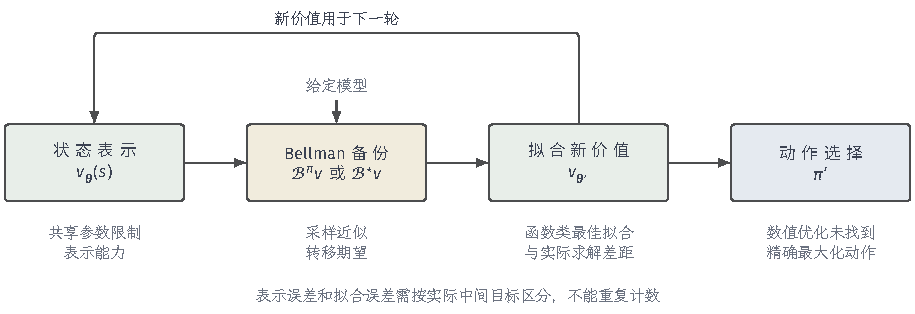
\includegraphics[width=154.961mm]{figures/10-reinforcement-learning/01-problems-and-solving/tikz/rl-planning-approximation-loop.pdf}
 \caption{全状态近似的共同计算接口。实线表示当前价值、备份目标、拟合结果与动作选择之间的计算依赖，外侧回路表示把新价值送往下一轮；下方分别标出表示、期望估计、拟合和动作优化可能产生的误差。给定模型仍是备份的输入。}
 \label{fig:rl-planning-approximation-loop}
\end{figure*}

这些计算仍以给定模型为输入。为了减少精确求和而使用模型样本，会留下有限样本的期望估计误差；模型本身若由真实交互学得，还会偏离环境规律，那是下一章要加入的另一层误差。本节只分析给定模型上的表示和求解，不把两种误差混称为来源不明的预测误差。

% Outline: 2.5.2
\subsection{跨状态近似价值的表示}
\label{sec:rl-planning-representation}

要用少数参数代替庞大的价值表，最直接的办法是让一整组状态共用同一个数值。\term{状态聚合}（state aggregation）就是这样一种分组表示：取一个映射$g:S\to\{1,\ldots,p\}$，令$v(s)=\theta_{g(s)}$，于是更新参数$\theta_i$会同时改变第$i$组所有状态的预测。分组的关键在于把“长期回报确实相近”的状态放在一起，而不能只凭几何上相邻就归为同组，否则被迫共享的误差会很大。

比硬分组更细的是\term{基函数展开}：让状态通过一组给定特征以加权和的形式贡献价值。用$\bm\phi(s)\in\mathbb R^p$表示特征向量、$\bm\theta$表示权重，写成
$\ v_{\bm\theta}(s)=\bm\phi(s)^\top\bm\theta$。
例如在网格中取$\bm\phi(s)=(1,x/4,y/3)^\top$，就只需保存3个参数便能为任意位置求值；代价是这样只能表示坐标的仿射函数，既不能任意指定11个格子的价值，也不会自动刻画“必须绕过障碍”这种非线性结构。若把特征取成各组的指示函数，基函数展开就退化为状态聚合。更一般的参数化函数（如神经网络）还能表达非线性关系，但它能表示哪些函数仍取决于网络结构和参数数量。

图~\ref{fig:rl-planning-aggregation}~用同一网格检查分组会丢失什么。按行聚合把障碍两侧的$(1,2)$和$(3,2)$放在同组，但两处最优价值约为$0.501527$和$0.801271$。共享常数不可能同时等于它们，最大误差至少为差值的一半，约$0.149872$。按到达终点的通道划组能够保留两侧差别，却没有证明组内所有价值相同；还须继续检查组内误差。

\begin{figure}[htbp]
 \centering
 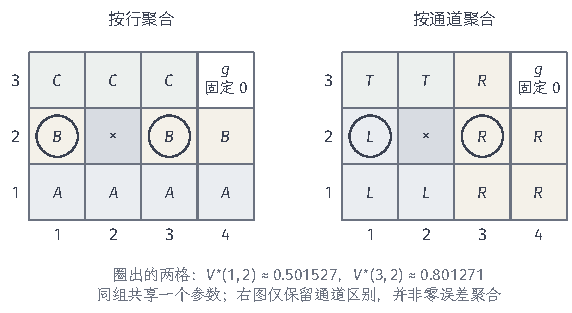
\includegraphics[width=96.788mm]{figures/10-reinforcement-learning/01-problems-and-solving/tikz/rl-planning-aggregation.pdf}
 \caption{同一基准网格的两种教学聚合。左图按行分成A、B、C组，右图按障碍周围的通道分成L、T、R组；非终点格的字母表示共享参数，终点价值固定为0，颜色仅作辅助。右图保留了障碍两侧的区别，但不是精确MDP同态或零误差聚合的声明。}
 \label{fig:rl-planning-aggregation}
\end{figure}

表~\ref{tab:rl-planning-representations}~分别比较一次价值求值与一次单状态参数更新所需的资源，其中$n_S=|S|$表示状态数。更灵活的函数类可能减小表示偏差，但投影迭代未必更稳定，数值优化也未必能找到最佳拟合。

\begin{table*}[htbp]
 \centering
 \small
 \begin{tabularx}{\linewidth}{@{}lcc>{\raggedright\arraybackslash}X@{}}
  \toprule
  表示 & 参数存储 & 求值／单样本更新 & 表达范围与限制\\
  \midrule
  全状态表 & $O(n_S)$ & $O(1)$／$O(1)$ & 可独立表示每个状态，不含模型存储\\
  $p$组聚合 & $O(p)$ & $O(1)$／$O(1)$ & 假设组索引可常数时间取得；组内差别全部丢失\\
  $p$维稠密线性特征 & $O(p)$ & $O(p)$／$O(p)$ & 只能表示特征张成空间；未计特征构造和批量解方程\\
  一般参数化函数 & 参数数$p_\theta$ & 依计算图而定 & 前向与反向代价须按架构计数；非凸拟合与泛化另需分析\\
  \bottomrule
 \end{tabularx}
 \caption{价值表示的资源口径。一次函数求值不包括Bellman备份所需的多后继求值；动作价值$q(s,a)$若为每个动作单独输出，还需计入动作维。}
 \label{tab:rl-planning-representations}
\end{table*}

% Outline: 2.5.3
\subsection{策略的近似价值评估}
\label{sec:rl-planning-approximate-evaluation}

固定策略$\pi$和线性函数空间$\mathcal F$后，目标是在这个有限表示里尽量逼近它的真实价值$V^\pi$。这里出现一个现实困难：如果真实价值$V^\pi$已知，直接拿状态—真实价值对$(s,V^\pi(s))$作回归即可，但规划时未知的恰恰就是$V^\pi$；我们真正拿得到的，只是由模型确定的Bellman关系。因此需要区分几种“在不知道$V^\pi$时仍可计算”的近似目标。为比较它们，先固定状态权重$\xi(s)>0$、$\sum_s\xi(s)=1$，以
$\lVert v\rVert_\xi^2=\sum_s\xi(s)v(s)^2$计量加权平方大小。优化在$\mathcal F$中寻找对应误差最小的函数；投影则把一次备份的结果变成该加权距离下最接近的可表示函数。

\begin{definition}[三种近似评价对象]
 \label{def:rl-planning-projected-evaluation}
 给定状态动作有限、奖励有界且$0\leq\gamma<1$的时间齐次MDP，$\pi$为合法平稳策略，$V^\pi$为其折扣价值。设$\mathcal F\subseteq\mathbb R^{|S|}$是线性子空间，$\xi(s)>0$且$\sum_s\xi(s)=1$，$\Pi_\xi$为加权内积$\langle u,v\rangle_\xi=\sum_s\xi(s)u(s)v(s)$下到$\mathcal F$的正交投影。三种近似评价问题分别为
 \[
 \begin{array}{ll}
 \text{价值拟合：}&\displaystyle\min_{v\in\mathcal F}\lVert v-V^\pi\rVert_\xi^2,\\
 \text{残差最小化：}&\displaystyle\min_{v\in\mathcal F}\lVert v-\mathcal B^\pi v\rVert_\xi^2,\\
 \text{投影方程：}&v=\Pi_\xi \mathcal B^\pi v,\qquad v\in\mathcal F.
 \end{array}
 \]
 前两者最小化不同误差；第三者要求一次备份后投影回来不再改变$v$，并不要求原始Bellman残差为零。
\end{definition}

定义中的价值拟合直接缩小预测与$V^\pi$的差，残差最小化缩小预测与自身备份的差；投影方程则寻找备份再投影后的不动点。因此后两者不要求先取得各状态的真实价值$V^\pi(s)$作为拟合目标，也不保证给出第一种答案。在线性表示中，我们可以将投影方程化为关于参数的线性系统：用$\bm\Phi\in\mathbb R^{n_S\times p}$的第$s$行为$\bm\phi(s)^\top$，
$\bm D=\operatorname{diag}(\xi)$，并假设$\bm\Phi$列满秩。投影矩阵为
$\bm\Pi_\xi=\bm\Phi(\bm\Phi^\top\bm D\bm\Phi)^{-1}\bm\Phi^\top\bm D$。
将$\bm v=\bm\Phi\bm\theta$代入投影方程并乘$\bm\Phi^\top\bm D$，得到
\begin{equation}
 \underbrace{\bm\Phi^\top\bm D(\bm I-\gamma\bm T^\pi)\bm\Phi}_{\bm A}
 \bm\theta
 =\underbrace{\bm\Phi^\top\bm D\bm r^\pi}_{\bm b}.
 \label{eq:rl-planning-projected-system}
\end{equation}
式~\eqref{eq:rl-planning-projected-system}~把函数不变条件压缩成$p$个参数的方程。但$\bm\Phi$列满秩只保证投影矩阵中的逆存在，不自动保证这里的$\bm A$可逆。只有后者可逆，$\bm A^{-1}\bm b$才是唯一参数解；若奇异，还需检查有无解、怎样选解，或是否另加正则化。正则化是改变方程的求解选择，不是原方程无条件可解的证明。

\begin{example}[同一特征的三种答案]
 \label{ex:rl-planning-projection}
 构造一个独立的两状态、单动作教学模型，$\gamma=1/2$，
 \[
 \bm T^\pi=\begin{pmatrix}0&1\\0&1\end{pmatrix},\quad
 \bm r^\pi=\begin{pmatrix}1\\0\end{pmatrix},\quad
 \bm\Phi=\begin{pmatrix}1\\2\end{pmatrix},\quad
 \bm D=\tfrac12\bm I.
 \]
 精确价值为$(1,0)^\top$。价值拟合最小化
 $\tfrac12[(\theta-1)^2+4\theta^2]$，故$\theta=1/5$。
 原始残差为$(1+\theta,\theta)^\top-(\theta,2\theta)^\top=(1,-\theta)^\top$，
 所以残差最小化给$\theta=0$。

 对投影方程，
 $(\bm I-\gamma\bm T^\pi)\bm\Phi=(0,1)^\top$，
 因而$\bm A=1$、$\bm b=1/2$，解为$\theta=1/2$。
 若每轮先备份再投影，参数更新为
 $\theta^{(k+1)}=1/5+(3/5)\theta^{(k)}$，也收敛到$1/2$。
 三者不同不是数值误差，而是目标不同。
 取投影解$\theta=1/2$，有$v=(1/2,1)^\top$、$\mathcal B^\pi v=(3/2,1/2)^\top$，于是
 \[
   \mathcal B^\pi v-v=(1,-1/2)^\top\ne0,\qquad
   \bm\Phi^\top\bm D(\mathcal B^\pi v-v)=0.
 \]
 可表示的价值只能沿$\bm\Phi$方向变化，剩余差与这个方向正交，所以投影后更新为零，原始Bellman残差却仍非零。

\end{example}

直接解方程之外，也可以反复备份再投影，但精确评价的收敛证明还需要复合算子$\Pi_\xi \mathcal B^\pi$保持压缩。一个充分条件是$\xi$为$\bm T^\pi$的严格正平稳分布，即按这个分布转移一步后分布不变。此时由Jensen不等式，
\[
 \lVert\bm T^\pi v\rVert_\xi^2
 \leq\sum_s\xi(s)\sum_{s'}T^\pi(s,s')v(s')^2
 =\lVert v\rVert_\xi^2.
\]
第一个不等式说明平方的加权平均不小于平均后的平方，最后的等式使用$\xi$的平稳性。正交投影在同一$\xi$范数下也不放大距离，二者复合再乘$\gamma$，便得到压缩和唯一投影不动点。例~\ref{ex:rl-planning-projection}~并无严格正平稳权重，但其参数更新斜率$3/5<1$直接给出收敛；刚才列的是充分条件，不是必要条件。

一般权重未必满足平稳等式，而最小二乘投影在无穷范数下也未必不放大距离，所以不能默认备份再投影稳定。若还能算出原始残差的全状态上界，式~\eqref{eq:rl-planning-evaluation-residual}~仍可为拟合结果提供价值误差证书；仅有投影残差为零则不够。只有模型样本时，残差梯度还涉及同一状态动作下如何组合独立后继样本，称为双重采样问题，由第~\ref{chap:rl-learning}~章展开。

% Outline: 2.5.4
\subsection{基于近似价值的策略改进}
\label{sec:rl-planning-approximate-improvement}

上一小节解决的是“在给定函数类里如何评价一条固定策略”，现在要用这个近似评价反过来改动作。这里有两种保存方式：若保存的是状态价值$v$，行动时还需借助模型把它换算成各动作可直接比较的量
$R(s,a)+\gamma T_av$，其中$T_av=\sum_{s'}T(s'\mid s,a)v(s')$；
若保存的就是动作价值$q(s,a)$，则可在合法动作中直接比较$q$、省去行动时的一步期望计算，但$q$估得准不准仍取决于学习质量。还要注意，即使假定估值本身完全给定，实际的数值优化也可能因为种种原因没有真正取到最大值；因此有必要把“价值估得准不准”和“动作有没有选对”这两类误差分开计量。

\begin{definition}[近似贪心误差]
 \label{def:rl-planning-greedy-error}
 给定时间齐次折扣MDP，其状态集$S$有限，各合法动作集$\mathsf A(s)$有限且非空，期望奖励$R(s,a)$为有限实数，$0\leq\gamma<1$。给定状态函数$v:S\to\mathbb R$及合法平稳策略$\pi'$，相对于$v$的模型贪心误差为
 \[
 \eta(v,\pi')=\lVert \mathcal B^*v-\mathcal B^{\pi'}v\rVert_\infty.
 \]
 因$\mathcal B^*v\geq \mathcal B^{\pi'}v$，它衡量实际动作选择比精确最大化少了多少一步备份价值。对给定动作价值$q$，对应地考察
 \[
  \sup_s\left[\max_{a\in\mathsf A(s)}q(s,a)-\sum_{a\in\mathsf A(s)}\pi'(a\mid s)q(s,a)\right].
 \]
\end{definition}

这里的无穷范数或上确界覆盖所有状态，比较方向是实际策略的备份比合法动作最大值少多少，避免某个状态的选择误差被平均掉。即使精确最大化$q$，动作价值估计也可能不准确。

这种比较动作选择误差的思路也可推广到连续动作，但此时须先给出合法动作集，再确认比较基准是能够取到的最大值，还是只能逼近的上确界。确定基准后，即使$v$准确，数值求解选出的动作也可能比该基准少一部分备份价值。因此有限动作的枚举与连续动作的数值优化应分别说明，后者还须给出约束、优化器和精度。上面的正式定义及后续误差推导仍采用有限MDP条件，并未据此自动获得连续动作下的全部保证。

估值和动作选择都可以放进迭代循环，但位置不同会改变每轮所求的对象。表~\ref{tab:rl-planning-approximate-loops}~用同一组评价、拟合和改进操作对照三种安排；$\mathcal F$为选定函数类，拟合用该类中的函数近似备份目标。特别是最优备份内部选了一次动作，不等于已经精确评价这份策略的长期价值。

\begin{table*}[htbp]
 \centering
 \small
 \begin{tabularx}{\linewidth}{@{}l>{\raggedright\arraybackslash}X>{\raggedright\arraybackslash}X@{}}
  \toprule
  循环 & 每轮备份与拟合 & 动作选择的位置\\
  \midrule
  近似策略迭代 & 固定$\pi^{(k)}$，用若干次评价备份及拟合得到$v^{(k)}\approx V^{\pi^{(k)}}$ & 评价结束后对$v^{(k)}$近似贪心\\
  近似价值迭代 & 一次$\mathcal B^*v^{(k)}$后拟合一次，得$v^{(k+1)}\in\mathcal F$ & 每次最优备份内部都比较动作\\
  修改策略迭代 & 先取$\pi^{(k+1)}$，再做$m_k$次$\mathcal B^{\pi^{(k+1)}}$；近似版本还需注明每次或最后拟合 & 每个外层循环开始时一次\\
  \bottomrule
 \end{tabularx}
 \caption{共享接口下的不同循环。$m_k=1$且没有拟合时，修改策略迭代退化为价值迭代；最优备份不意味着已经精确评价了所选策略。}
 \label{tab:rl-planning-approximate-loops}
\end{table*}

用一个只剩一步的教学问题检查误差会怎样改变选择。真实动作价值为$Q(a)=0.50,Q(b)=0.49$，若估计误差分别为$-0.01,+0.01$，就得到$q(a)=0.49,q(b)=0.50$，精确贪心也会选$b$。最大估值误差为$0.01$，已经足以翻转两动作的排序；若旧策略选$a$，新策略真实回报反而下降$0.01$。所以近似改进不继承每轮单调提高的无条件保证，下一步要把评价误差和动作选择误差带入长期性能分析。

% Outline: 2.5.5
\subsection{误差传播与策略性能损失}
\label{sec:rl-planning-error-propagation}

在近似迭代里，每一次备份都可能同时受到表示能力不足、采样噪声和数值优化的影响。为了分析这些误差如何一轮轮传播，先把“实际更新”与“对同一当前价值函数$v^{(k)}$、使用同一给定模型所得的理想最优备份”作差，写成
$v^{(k+1)}=\mathcal B^*v^{(k)}+e^{(k)}$。
这里的$e^{(k)}$有意做成一个“大口袋”，装下本轮相对理想备份的全部误差；若需要区分来源，可以在理想备份目标与实际更新所得的$v^{(k+1)}$之间依次插入若干中间量，相邻两项之差分别对应动作优化误差、期望估计误差、表示不足和拟合求解误差，再用三角不等式给总差一个上界。比较时必须始终使用同一范数：在加权二范数下的最佳拟合，未必也是最大状态误差最小的那个拟合。

图~\ref{fig:rl-planning-error-flow}~将旧误差与新误差分开：理想算子的压缩性减小上一轮的价值误差，本轮$e^{(k)}$又使结果偏离理想备份。若动作优化误差已计入$e^{(k)}$，就不能在总界$\delta$中重复加入；最终从价值表另行提取策略所产生的近似贪心误差，才是另一处需要计量的误差。下面用每轮全状态总误差不超过$\delta$的条件，控制价值和输出策略的性能。

\begin{figure}[htbp]
 \centering
 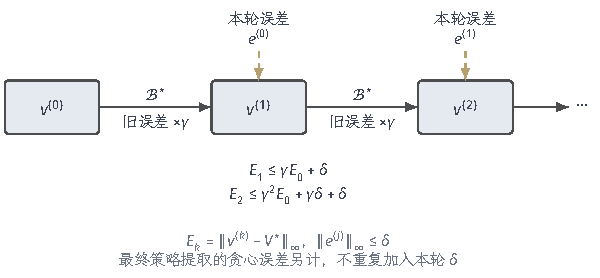
\includegraphics[width=101.533mm]{figures/10-reinforcement-learning/01-problems-and-solving/tikz/rl-planning-error-flow.pdf}
 \caption{近似价值迭代的误差传播。横向每经过一次理想Bellman备份，旧误差乘$\gamma$；上方$e^{(k)}$在各轮注入。因此第$j$轮的误差对第$k$轮的贡献按$\gamma^{k-1-j}$衰减，而每轮都持续注入的误差不会消失。}
 \label{fig:rl-planning-error-flow}
\end{figure}

\begin{theorem}[近似价值迭代的统一误差界]
 \label{thm:rl-planning-avi-error}
 设时间齐次MDP的状态动作有限、各动作集非空、奖励有界，且$0\leq\gamma<1$，$V^*$为最优折扣价值。给定$\delta\geq0$及状态函数序列$(v^{(k)})_{k\geq0}$，若每轮满足$\lVert v^{(k+1)}-\mathcal B^*v^{(k)}\rVert_\infty\leq\delta$，则
 \begin{equation}
 \lVert v^{(k)}-V^*\rVert_\infty
 \leq\gamma^k\lVert v^{(0)}-V^*\rVert_\infty
       +\frac{\delta(1-\gamma^k)}{1-\gamma}.
 \label{eq:rl-planning-avi-error}
 \end{equation}
 若输出策略$\pi^{(k)}$对$v^{(k)}$的贪心误差不超过$\eta$，其真实性能满足
 \[
 \lVert V^*-V^{\pi^{(k)}}\rVert_\infty
 \leq\frac{2\gamma\lVert v^{(k)}-V^*\rVert_\infty+\eta}{1-\gamma}.
 \]
\end{theorem}
\begin{proof}
 记$E_k=\lVert v^{(k)}-V^*\rVert_\infty$。插入$\mathcal B^*v^{(k)}$并使用压缩性，
 \[
 E_{k+1}\leq
 \lVert v^{(k+1)}-\mathcal B^*v^{(k)}\rVert_\infty+
 \lVert \mathcal B^*v^{(k)}-\mathcal B^*V^*\rVert_\infty
 \leq\delta+\gamma E_k.
 \]
 连续代入得到
 $E_k\leq\gamma^kE_0+\delta\sum_{j=0}^{k-1}\gamma^j$，计算几何和即为第一式。

 提取策略时，插入$\mathcal B^*v^{(k)}$及$\mathcal B^{\pi^{(k)}}v^{(k)}$，两者差至多$\eta$。其余两项分别用最优算子和策略算子的压缩性控制，得到
 \[
 \lVert V^*-V^{\pi^{(k)}}\rVert_\infty
 \leq 2\gamma E_k+\eta+
       \gamma\lVert V^*-V^{\pi^{(k)}}\rVert_\infty.
 \]
 移项即得第二式；$\eta=0$时正好回到精确贪心性能界。
\end{proof}

在教学参数$\gamma=0.9$、每轮统一误差$\delta=0.001$下，几何累积给出渐近价值误差上界$0.01$，再转成精确贪心策略的损失上界为$0.18$。误差先在价值迭代中累积，又在长期执行的性能比较中放大；两个分母各有来源。这些是可能保守的解析上界，不表示实际网格正好损失相应数值。

上界使用最大状态误差，而拟合目标可能只控制加权二范数，两种精度不能直接交换。假设一个状态在拟合分布中仅有$10^{-6}$概率，误差为1，其他状态误差为0，加权二范数仍只有$10^{-3}$。部署若恰好从这个状态开始，低权重下的小误差指标就没有控制初始决策。要将加权误差转成性能界，还需限制部署占用相对拟合分布的偏移，例如要求覆盖并控制密度比，即同一状态在两分布中的概率之比。原分布给零概率的状态，也不能靠增加该分布上的样本数覆盖。生成模型下拟合价值迭代的有限时间分析因此保留函数类的逼近能力，以及相关未来状态分布相对拟合分布的密度比控制条件。具体控制哪些未来状态分布、怎样聚合它们的密度比，取决于所用的误差传播界，不能只检查最终策略的一份占用分布\scite{rl2-munos2008-fitted}

近似策略迭代每轮评价的是一份变化中的策略，不是直接近似一次$\mathcal B^*$更新，所以式~\eqref{eq:rl-planning-avi-error}~的假设不再对应。我们改为控制每轮估值离当前策略真实价值的最大误差。若
$\lVert v^{(k)}-V^{\pi^{(k)}}\rVert_\infty\leq\varepsilon$，
改进误差不超过$\eta$，则
$\mathcal B^{\pi^{(k+1)}}V^{\pi^{(k)}}\geq \mathcal B^*V^{\pi^{(k)}}-\beta
\geq V^{\pi^{(k)}}-\beta$，
其中$\beta=2\gamma\varepsilon+\eta$。比较$\mathcal B^*v^{(k)}$与$\mathcal B^{\pi^{(k+1)}}v^{(k)}$给出$\eta$，把两边估值换回真实$V^{\pi^{(k)}}$各付出至多$\gamma\varepsilon$，便得到这项不等式。
为把一次可能下降的备份转成新策略真实价值的下降界，利用恒等式
\[
 V^{\pi'}-V^\pi
 =(\bm I-\gamma\bm T^{\pi'})^{-1}(\mathcal B^{\pi'}V^\pi-V^\pi)
\]
这里$\pi=\pi^{(k)}$、$\pi'=\pi^{(k+1)}$。逆矩阵的几何级数非负，行和为$1/(1-\gamma)$，因而备份下降至多$\beta$时，真实价值满足$V^{\pi'}\geq V^\pi-\beta/(1-\gamma)$。
再比较新策略与最优价值，在两者之间插入$\mathcal B^*V^\pi$和$\mathcal B^{\pi'}V^\pi$，逐状态得到
\[
\begin{aligned}
 V^*-V^{\pi'}
 &=\mathcal B^*V^*-\mathcal B^{\pi'}V^{\pi'}\\
 &\leq\gamma\lVert V^*-V^\pi\rVert_\infty
       +\beta+\gamma\bm T^{\pi'}(V^\pi-V^{\pi'})\\
 &\leq\gamma\lVert V^*-V^\pi\rVert_\infty+\frac{\beta}{1-\gamma}.
\end{aligned}
\]
由于$V^*\geq V^{\pi'}$，对状态取最大值得到保守递推
$\lVert V^*-V^{\pi^{(k+1)}}\rVert_\infty
\leq\gamma\lVert V^*-V^{\pi^{(k)}}\rVert_\infty+\beta/(1-\gamma)$，
将这项递推展开为几何和，渐近损失至多$\beta/(1-\gamma)^2$。这里控制的是每轮相对\emph{当前策略真实价值}的评价误差；AVI，即近似价值迭代，控制的则是一次最优备份误差，二者不能混用。更细的加权范数和不同迭代安排的误差传播可见Farahmand等\scite{rl2-farahmand2010-errors}

% Outline: 2.6
\section{可计算性与复杂度边界}
\label{sec:rl-planning-complexity}

同样一步Bellman备份，背后的实际代价可能天差地别：有的是对一行已知概率逐项求和，有的要反复采样，连续动作还要调用数值优化器。它们写在伪代码里可能都只是“一行更新”，但若不统一计量单位，就无法判断一个算法究竟快还是慢。沿用前面的精确表项、解析动力学或生成模型访问协议，可以分别计算各种方法为了求得价值表、策略或根动作及相应精度所需要的算术运算、存储空间与模型查询次数；只有这些单位先固定下来，“迭代次数少”或“复杂度与状态数无关”这类说法才有确切含义。

% Outline: 2.6.1
\subsection{复杂度指标与模型访问}
\label{sec:rl-planning-access-complexity}

为了比较“一次完整扫描”和“一棵采样树”的代价，先要分清四类资源各计什么。\term{算术运行时间}数加法、乘法等基本运算的次数，回答计算量多大；\term{存储复杂度}数同一时刻需要同时保留的模型、价值、策略和搜索节点，回答要占多少内存；\term{并行深度}数即便有无限多个处理器、仍然必须按顺序完成的依赖层数，回答并行之后最快能多快；\term{模型调用复杂度}则数向外部模型接口发起查询的次数，回答要消耗多少（往往昂贵的）仿真或真实采样。增加处理器可以在依赖允许的范围内缩短延迟，却不会自动减少总运算量或总样本数。

表~\ref{tab:rl-planning-access-models}~对应四种模型表示的基本操作。读取一个表项、遍历一个后继集合和取得一个随机样本，返回的转移概率、后继值或单次奖励记录不同；因此必须先规定一次访问指什么，再比较调用次数。

\begin{table*}[htbp]
 \centering
 \small
 \begin{tabularx}{\linewidth}{@{}l>{\raggedright\arraybackslash}X>{\raggedright\arraybackslash}X@{}}
  \toprule
  模型表示 & 基本访问操作 & 一次备份仍需付出的代价\\
  \midrule
  显式稠密转移表 & 读取一个概率或奖励表项 & 对$n_S$个后继求和；需要整个模型的存储\\
  稀疏转移表 & 遍历一个状态动作的非零后继 & 对$b$个后继求和，并读取对应价值\\
  解析动力学 & 计算状态转移或积分表达式 & 单次函数代价依公式而定；有公式不等于积分可解析\\
  生成模型 & 给定$(s,a)$取得一个独立$(r,s')$ & 用样本均值估计期望；还须计样本数与失败概率\\
  \bottomrule
 \end{tabularx}
 \caption{不同模型访问协议的计数单位。表中$b$表示非零后继数；生成模型的一次查询通常只产生一个后继，不能与遍历整行概率等价计数。}
 \label{tab:rl-planning-access-models}
\end{table*}

以同一个后继期望$T_av$为例，稀疏精确模型要读取$b$个后继价值并加权求和，没有采样误差。生成模型用$m$个后继样本的均值近似它，调用代价随$m$增加，精度则要附带失败概率。即使$m<b$，也只是以更少查询换取近似结果；比较同精度下的速度，还要说明两者误差标准如何对齐。

所求价值表、策略或根动作的精度要求也要固定。全状态价值精度约束每个坐标，给定$\mu_0$的策略精度约束其回报差，当前状态选择则只需控制一个根决策的损失。三者不同，不能共用所有下界：写出$n_S$维显式价值表本身至少需要$\Omega(n_S)$次写入，而输出一个根动作不需要写出这张表。

一次基本算术运算按单位成本计数，前提是将参与运算的数视为可在单步处理。模型编码的读取、价值表或策略等结果的表示长度，以及运算数目分别给出资源要求，不能用迭代次数代替全部成本。若进一步计算位复杂度，即处理数字的二进制编码所需的工作，还要考虑转移概率的编码位长、目标精度和精确消元中的分子分母增长。多项式算术步数并不意味着每一步的位运算都只需常数成本；采用浮点实现时，舍入误差也应纳入残差证书。

% Outline: 2.6.2
\subsection{全状态动态规划的计算代价}
\label{sec:rl-planning-dp-complexity}

先数一次精确最优Bellman扫描的工作。设状态数为$n_S$，每处合法动作至多$n_A$，实际状态动作对的平均非零后继数为$b$。扫描逐个状态枚举动作，再遍历各动作的后继；状态动作对至多$n_Sn_A$个，每对平均付出$b$次后继计算，因此代价上界为
\begin{equation}
 O(n_Sn_Ab).
 \label{eq:rl-planning-sweep-cost}
\end{equation}
若转移稠密，$b=n_S$，一次扫描便为$O(n_S^2n_A)$。稀疏模型及奖励占$O(n_Sn_Ab)$存储，价值表占$O(n_S)$；确定性策略每状态只存一个动作索引，共$O(n_S)$个字，随机策略则至多存$O(n_Sn_A)$个概率。同步更新多留一张价值表，但价值存储阶仍为$O(n_S)$，模型存储要另外计入。

总运行时间还要乘扫描轮数。压缩性给出第$k$轮误差至多$\gamma^kE_0$，其中$E_0$界住初始误差；要使它不超过$\varepsilon$，在$0<\gamma<1$、$0<\varepsilon<E_0$时解这个不等式，得到充分轮数
\begin{equation}
 k\geq\left\lceil\frac{\log(E_0/\varepsilon)}{-\log\gamma}\right\rceil.
 \label{eq:rl-planning-iteration-count}
\end{equation}
从零初始化时，有界回报给出$E_0=R_{\max}/(1-\gamma)$。利用$-\log\gamma\geq1-\gamma$，可以进一步采用较保守的
$O((1-\gamma)^{-1}\log(E_0/\varepsilon))$轮数上界。$\gamma$越接近1，未来影响衰减越慢，达到同一精度可能需要更多轮。边界也要分开：$\gamma=0$时一次备份已最优，$\varepsilon\geq E_0$时初值已满足精度，都无须使用对数式。

表~\ref{tab:rl-planning-dp-costs}~将各操作的单轮成本与轮数要求分开。固定确定性策略只使用一个动作，稠密随机策略还要按动作概率混合，或提前构造$\bm T^\pi,\bm r^\pi$。若直接解稠密$n_S$阶评价方程，常规消元需$O(n_S^3)$运算及$O(n_S^2)$存储。稀疏消元可能产生填充，即原本为零的位置在消元中变成非零，所以不能仅将$b$代入稠密立方公式，就认定得到稀疏求解代价。

\begin{table*}[htbp]
 \centering
 \small
 \begin{tabularx}{\linewidth}{@{}l>{\raggedright\arraybackslash}X>{\raggedright\arraybackslash}X@{}}
  \toprule
  操作 & 单轮算术代价 & 轮数或输出条件\\
  \midrule
  固定确定性策略的迭代评价 & 一次固定策略扫描$O(n_Sb_\pi)$ & $b_\pi$为所选动作平均后继数；轮数由评价压缩或残差确定\\
  策略改进 & $O(n_Sn_Ab)$ & 只比较一次动作；不包括评价\\
  价值迭代 & $O(n_Sn_Ab)$ & 达到价值误差的轮数见式~\eqref{eq:rl-planning-iteration-count}\\
  精确策略迭代 & 稠密评价$O(n_S^3)$加改进；模型混合另计 & 外层轮数依问题而变；有限终止论证只给有限策略数的粗界\\
  \bottomrule
 \end{tabularx}
 \caption{全状态动态规划的成本。$b_\pi$可能与所有动作平均的$b$不同；表中随机策略若未预先混合转移，评价扫描还需计入动作枚举。}
 \label{tab:rl-planning-dp-costs}
\end{table*}

前面的有限终止证明只用到了确定性策略总数$\prod_s|\mathsf A(s)|$。它对$n_S$可能指数增长，因此既不是紧的轮数分析，也不是多项式时间结论。若要作更细比较，必须说明策略迭代的具体规则、折扣是否固定，以及复杂度定理所计的模型编码规模与运算。

同步扫描内，各状态动作的后继求和可以并行。令$b_{\max}$为最大非零后继数，树状求和再比较动作最大值的依赖深度为$O(\log(1+b_{\max})+\log(1+n_A))$；这里必须用最大值而不是平均$b$，因为并行延迟由最长计算链决定。第$k+1$轮仍使用第$k$轮的价值，所以有足够处理器也不能将所有轮次同时完成。

% Outline: 2.6.3
\subsection{时域、分支与搜索复杂度}
\label{sec:rl-planning-search-complexity}

局部搜索省去了全状态扫描，却可能反复展开同一位置的不同历史。为数完整树的规模，固定每处$A$个动作、每个动作$B$个随机后继，并以动作执行次数计深度$H$。每层状态节点增加$AB$倍，因此状态节点总数为
$\sum_{h=0}^{H}(AB)^h$，非叶状态处的动作节点数为
$A\sum_{h=0}^{H-1}(AB)^h$。
当$AB>1$时，前者为$[(AB)^{H+1}-1]/(AB-1)$，随深度指数增长；$AB=1$时则只有一条长度$H$的链，不能使用分母为0的几何和形式。

若两条历史到达同一网格位置，且剩余步数相同，马尔可夫性保证它们面对同一个后继子问题。于是可合并相同的$(s,\text{剩余深度})$，用动态规划图复用结果；连终端层在内至多有$(H+1)n_S$个时层状态，其中至多$Hn_S$个需要备份。合并要支付状态识别与存储成本，利用的是当前状态与剩余步数对后继子问题的充分性，而非删除真实随机后果。连续状态很少精确重复时，这种复用可能收益有限。

表~\ref{tab:rl-planning-search-costs}~回到同一棵搜索树，比较截断、采样、叶值、自适应访问和状态合并各省去什么工作。稀疏采样将每动作后继数$B$替换为$m$，仍保留$(Am)^H$的深度依赖；MCTS只展开访问到的节点，但减少节点不等于普遍改善固定预算下的最坏决策误差。

\begin{table*}[htbp]
 \centering
 \small
 \begin{tabularx}{\linewidth}{@{}l>{\raggedright\arraybackslash}X>{\raggedright\arraybackslash}X@{}}
  \toprule
  手段 & 减少的计算 & 误差及额外条件\\
  \midrule
  深度截断 & 删除$H$步之后的展开 & 尾和或$\gamma^H\varepsilon$终端误差；短视不可逆动作仍危险\\
  稀疏采样 & 每个动作只抽$m$个后继 & 样本均值及递归误差；独立生成模型、置信度和树规模\\
  叶值近似 & 用一次求值替代叶外模拟 & 叶值必须在到达区域准确；预计算和训练代价另计\\
  MCTS & 将查询集中于被选择的分支 & 回报非平稳、叶值偏差与探索条件；选择性展开不是普遍最坏界\\
  状态合并 & 复用相同状态及剩余深度的计算 & 要求状态表示足以确定剩余决策问题的转移与奖励规律，并支付索引与存储成本\\
  \bottomrule
 \end{tabularx}
 \caption{搜索预算的节省对象。不同手段可以组合，但组合后的误差应按实际接口重新分析。}
 \label{tab:rl-planning-search-costs}
\end{table*}

若一次MCTS模拟至多走$H$层，每层只抽一个后继，叶值评估又需$L$次模型调用，则调用至多为$H+L$，$N$次模拟至多为$N(H+L)$。这个计数不含动作枚举、网络求值或连续优化，也没有说明误差随$N$减小多快。模拟长度随机时，还应分别报告期望调用和尾部延迟；平均用时小于预算不保证每次都在截止时间内返回。

% Outline: 2.6.4
\subsection{计算下界}
\label{sec:rl-planning-lower-bounds}

前面给出的都是上界：我们构造了某个算法，并数清它需要多少工作。但上界无法回答“还能不能更省”。要证明某类问题在给定接口下至少要付出多少代价，常用的办法是构造\term{不可区分问题对}：设置两个环境，让它们对算法已经发起的查询返回相同记录，却在尚未查询的奖励表项或后继分支上有所不同，使真正的最优动作也不同。只凭这份共同记录，算法无法确定自己面对哪一个环境；若必须在两者中都精确选对，就须继续取得能够区分它们的查询记录。对允许随机失败的算法，则要控制两环境下查询记录分布的差别及相应的判别错误概率。这样才能分别得到精确表项读取和随机样本辨识的资源下界。

先隔离精确表项的读取代价。一个单步问题有$n_A$个动作，算法已读奖励都为0，未查动作中可能有一个奖励为1。若还剩至少两个未查动作，就可以分别把唯一奖励1放在它们上面，得到相同读取记录和不同最优动作。因此要求精确最优的确定性算法，最坏至少要查$n_A-1$个表项；扫描全表给出$O(n_A)$上界。奖励没有随机性，取得未查动作的奖励值仍须付出读取成本。

换成生成模型，一次读到的奖励不再确定其期望，我们就要数样本辨识的代价。考虑单状态、单步、两动作，即$H=1$、没有后续奖励，也等价于$\gamma=0$。奖励在$[0,1]$内，动作$a_1$恒得$1/2$，动作$a_2$在模型$M_+$和$M_-$中分别服从
$\operatorname{Bernoulli}(1/2+2\varepsilon)$和
$\operatorname{Bernoulli}(1/2-2\varepsilon)$，其中$0<\varepsilon\leq1/8$。
要求算法输出一个确定性根动作，并在模型样本及自身随机性下，以至少$1-\alpha$的概率使该动作期望奖励离最优不超过$\varepsilon$，其中$0<\alpha<1/4$。两模型的最优动作相反，选错会损失$2\varepsilon$，所以达到精度要求就必须分辨它们。

为计算自适应奖励查询积累的对数似然证据，令$T$为停止查询的时刻，$A_k,X_k$为第$k$次查询的动作与奖励，$\widehat a$为最终根动作。完整记录包含独立于环境的内部随机种子，以及$(A_k,X_k)_{k=1}^T$、$T$和$\widehat a$；记它在两模型下的分布为$\mathbb P_+,\mathbb P_-$。要求$T$在两模型下几乎必然有限；若$\mathbb E_+N_2=\infty$，下界已经成立，下面只需考虑有限期望，其中$N_2=\sum_{k=1}^T\mathbf1\{A_k=a_2\}$。记录分布的KL仍是按前一分布平均对数似然比，即$D_{\mathrm{KL}}(\mathbb P_+\Vert\mathbb P_-)=\mathbb E_+\log(d\mathbb P_+/d\mathbb P_-)$，其中$d\mathbb P_+/d\mathbb P_-$表示同一记录在两模型下的似然比。

给定同一已有历史，同一个算法的动作选择、停止和输出规则相同，内部种子的分布也相同，因此这些因素在记录似然比中相消。$a_1$的奖励在两模型下相同，也不贡献；只有每次$a_2$的奖励留下一个似然比。令$p=1/2+2\varepsilon$、$q=1/2-2\varepsilon$，$f_p,f_q$为相应Bernoulli概率质量函数，下面将Bernoulli分布简记为$\operatorname{Ber}$。于是
\[
 \begin{aligned}
 \log\frac{d\mathbb P_+}{d\mathbb P_-}
 &=\sum_{k=1}^{T}\mathbf1\{A_k=a_2\}
          \log\frac{f_p(X_k)}{f_q(X_k)},\\
 D_{\mathrm{KL}}(\mathbb P_+\Vert\mathbb P_-)
 &=\mathbb E_+N_2\,
       D_{\mathrm{KL}}(\operatorname{Ber}(p)\Vert\operatorname{Ber}(q)).
 \end{aligned}
\]
第二式先对每次查询前的历史取条件期望，再对查询次数求和；这里单次对数比有界，$\mathbb E_+N_2$有限，保证求和与期望可交换。停止时间下的这类换测度等式见Kaufmann等附录A式(18)\scite{rl3-kaufmann2016complexity}

利用$\log z\leq z-1$分别界住Bernoulli散度的两项，可得
\[
 \begin{aligned}
 D_{\mathrm{KL}}(\operatorname{Ber}(p)\Vert\operatorname{Ber}(q))
 &\leq\frac{(p-q)^2}{q(1-q)}
 \leq\frac{256}{3}\varepsilon^2.
 \end{aligned}
\]
最后一步使用$p-q=4\varepsilon$、$q\in[1/4,1/2)$和$q(1-q)\geq3/16$。取$C=256/3$，总记录散度便至多为$C\varepsilon^2\mathbb E_+N_2$，这说明每个样本能积累的分布差别很少。

再以事件$B=\{\widehat a=a_1\}$把输出看作二元检验：$\mathbb P_+(B)$和$\mathbb P_-(B^{\mathrm c})$分别是两模型中的错误概率。两种Bernoulli参数均在$(0,1)$内，奖励支持相同；结合共同的算法规则及两模型下有限的$T$，记录分布互相绝对连续，即任一记录事件在一个模型下概率为0时，另一个也为0。在此条件下，检验界给出
\[
 \mathbb P_+(B)+\mathbb P_-(B^{\mathrm c})
 \geq\tfrac12\exp[-D_{\mathrm{KL}}(\mathbb P_+\Vert\mathbb P_-)].
\]
这里使用Kaufmann等附录A引理20中的事件形式\scite{rl3-kaufmann2016complexity}
成功要求使左侧不超过$2\alpha$，故记录散度至少为$\log(1/(4\alpha))$。与上界合并，得到
\[
 \mathbb E_+N_2\geq
 \frac{\log(1/(4\alpha))}{C\varepsilon^2}.
\]
这说明记录必须积累足够的分布差别，才能达到规定的检验成功率。对$\alpha\leq1/8$，所需样本阶为
$\Omega(\varepsilon^{-2}\log(1/\alpha))$。反过来，用固定次数独立样本估计$a_2$均值，与$1/2$比较，Hoeffding不等式给出同阶上界。若接口直接返回精确期望，只查一次就能区分二者，这条样本下界随即不适用。

再将困难放在未查搜索分支中，而不是奖励采样中。考虑深度$H$、每层$n_A\geq2$动作的完整确定性树，目标有限时域且不折扣。此前奖励都为0，$n_A^H$个终端叶子中恰有一个得1，其余为0；结构已知，但只能逐次精确查询叶奖励，没有可利用的参数关系或内部节点摘要。要求以至少$2/3$概率输出损失不超过$\varepsilon<1/2$的确定性根动作，也就是选中包含奖励叶的根分支。

若把唯一奖励叶在$n_A^H$个位置均匀放置，至多$q$次查询发现它的概率不超过$q/n_A^H$。固定算法的随机种子后，在所有查询都返回0的记录上，算法只能输出某个根分支；该分支最多包含全部叶子的$1/n_A$，所以“未发现且猜对”这一联合事件的概率至多为$1/n_A$。对随机种子取平均，界仍成立。因此总体成功率不超过$q/n_A^H+1/n_A$，要达到$2/3$，必有$q\geq n_A^H/6$。这个对奖励叶位置均匀抽样的论证，也推出至少一种奖励叶配置上的随机算法预算下界；扫描全部叶子则给匹配上界。指数困难来自没有结构的叶奖励表，不能把它推广为所有简洁模型的不可解性，或声称共享状态的网格必然需要同样多的查询。

表~\ref{tab:rl-planning-bounds}~分别将三个受限问题族的下界与同条件上界并列。每行数量级匹配，含义是该行指定任务所需资源的阶已确定；行间接口、精度和成功概率不同，不能合并为一般MDP的统一最优复杂度。

\begin{table*}[htbp]
 \centering
 \small
 \begin{tabularx}{\linewidth}{@{}>{\raggedright\arraybackslash}Xcc>{\raggedright\arraybackslash}X@{}}
  \toprule
  问题配置、目标与查询接口 & 下界 & 同条件上界 & 匹配范围\\
  \midrule
  单步$n_A$动作、精确奖励表、精确最优动作 & $\Omega(n_A)$ & $O(n_A)$ & 表项读取次数，不是随机样本数\\
  单步两动作Bernoulli模型、$\varepsilon\leq1/8$、$\alpha\leq1/8$ & $\Omega(\varepsilon^{-2}\log(1/\alpha))$ & $O(\varepsilon^{-2}\log(1/\alpha))$ & 独立生成样本；常数因子未追求一致\\
  完整确定树、唯一奖励叶、根动作成功率$2/3$ & $\Omega(n_A^H)$ & $O(n_A^H)$ & 精确叶奖励查询；不含到叶路径执行成本\\
  \bottomrule
 \end{tabularx}
 \caption{三个受限问题族中的上、下界。它们分别隔离奖励表项读取、统计辨识和搜索宽深度，不能合并为一个适用于所有MDP的复杂度公式。}
 \label{tab:rl-planning-bounds}
\end{table*}

两臂下界还没有说明一般有限MDP的状态数和长期传播怎样影响采样。考虑$n_S$个状态、每个状态$n_A$个动作的时间齐次折扣MDP，$0<\gamma<1$，奖励为已知确定性函数$R(s,a)\in[0,1]$。生成模型允许在任意指定的$(s,a)$独立采样后继；对每对查询$N$次，以后继计数的频率构造经验转移$\widehat T$，便得到一份可交给前面规划算法的经验MDP。用$\widehat V^\pi$和$\widehat V^*$表示该经验模型中的策略价值和最优价值，区别于真实环境中的$V^\pi,V^*$。

采样后不能只证明某份预先固定策略的估值准确，因为规划器会主动选择在这批记录上看起来最好的策略。Agarwal等处理了所选策略与经验转移之间的依赖，得到如下代表性样本保证：对$\varepsilon\in(0,1]$、$\delta\in(0,1)$，存在通用常数$c,C>0$，当
\begin{equation}
 \begin{aligned}
 N&\geq\max\left\{1,
   \frac{c\log\!\bigl(8n_Sn_A/[(1-\gamma)\delta]\bigr)}
        {(1-\gamma)^3\varepsilon^2}\right\},\\
 \|\widehat V^*-\widehat V^{\widehat\pi}\|_\infty
      &\leq\varepsilon_{\mathrm{opt}}
       \leq(1-\gamma)\varepsilon,
 \end{aligned}
 \label{eq:rl-planning-generative-rate}
\end{equation}
达到右侧精度的合法平稳策略$\widehat\pi$，以至少$1-\delta$的概率满足
$\|V^*-V^{\widehat\pi}\|_\infty\leq C\varepsilon$。
这里概率针对生成查询，内部规划器须确实达到所列全状态精度。这个状态价值结论需要保留动作选择的质量，不能仅由$Q^{\widehat\pi}$接近$Q^*$直接改写出来。取真实最优策略$\pi^*$，用$\widehat Q^\pi$表示同一策略在经验模型中的动作价值，则
\[
 \|V^*-V^{\widehat\pi}\|_\infty
 \leq \|Q^*-\widehat Q^{\pi^*}\|_\infty
       +\varepsilon_{\mathrm{opt}}
       +\|\widehat Q^{\widehat\pi}-Q^{\widehat\pi}\|_\infty.
\]
这是在两份真实价值之间插入$\widehat V^{\pi^*}$和$\widehat V^{\widehat\pi}$所得：首末两项比较同一策略在两个模型中的价值，可按该策略平均动作价值误差；中项由$\widehat V^{\pi^*}\leq\widehat V^*$及规划精度控制。强的经验状态价值条件也保证
$\|\widehat Q^*-\widehat Q^{\widehat\pi}\|_\infty
\leq\gamma\varepsilon_{\mathrm{opt}}$。
原分析同时控制上式首末两个动作价值估计误差，按所列$N$与内部精度即可得到$C\varepsilon$界；保留中项避免漏掉初始动作选错的损失。

按式\eqref{eq:rl-planning-generative-rate}左侧阈值的数量级选择正整数$N$，总查询数为$n_Sn_AN$，因而在隐藏对数因子的记法下为
$\widetilde O\!\left(n_Sn_A/[(1-\gamma)^3\varepsilon^2]\right)$；
将$\varepsilon$按常数缩小即可得到预先指定的策略误差。内部精度也随$1-\gamma$缩小，因为经验规划误差会通过后续执行放大\scite{rl2-agarwal2020-generative}

这条结果不要求先将整张转移表逐项估到很小的总变差。分析利用后继价值的方差，并通过将一个状态改为吸收状态的辅助模型，解除待评价价值与该状态转移样本之间的部分依赖；只对固定函数套一次集中界不够。经验模型随后可以调用价值迭代或其他达到所需精度的规划器，所以同一个外部样本率可以对应不同的内部运算和存储开销。极小极大率比较指定MDP类中最不利环境的样本需求，不等于每个具体网格都同样困难，也不是精确概率表的读取下界。真实在线交互通常还不能查询未到达状态，还须承担探索与可达性的代价。

% Outline: 2.7
\section{本章小结}
\label{sec:rl-planning-summary}

章首的问题现在可以分成两步回答：准确模型给出了计算长期后果的依据，所求价值表、策略或根动作及预算决定我们能算到哪里。在基准网格上，精确Bellman求解和占用量线性规划都得到同一个最优起点价值
$J(\pi^*)\approx0.421161$；前文定义并评价的均匀合法策略满足
$J(\pi_{\mathrm u})\approx-0.154754$。最优策略与均匀合法策略的回报差来自行动方式，而不是更换奖励或滑移规则。价值评价各状态的长期后果，占用量记录策略怎样分配折扣时间；二者由
$J(\pi)=(1-\gamma)^{-1}\sum_{s,a}d^\pi(s,a)R(s,a)$联系，所以归一化流量恢复为未归一化回报时，必须保留尺度系数。

进一步减少精确计算，要找到实际模型中的结构，而不是只辨认方法名称。LQR用动力学与成本保持二次价值，KL控制用受限转移和偏离费用使方程换元线性化；递减差分支持单调选择，独立子过程还须配合笛卡尔积动作才能直接分解。它们可以叠加，但动作约束、噪声机制或共享资源的改变也可能破坏原推导，使用时应回到对应条件检查。

资源仍不足时，可以局部搜索，也可以保存可复用的近似价值，二者能在叶值处结合。表~\ref{tab:rl-planning-method-choice}~按所求价值表、策略或根动作、模型访问协议和资源归纳这种选择，并列出应检查的误差依据。深度限制留下尾部误差，有限样本留下期望估计误差，函数表示与拟合留下跨状态误差，动作求解还可能留下选择误差；减小其中一项并不自动减小其他项。

\begin{table*}[htbp]
 \centering
 \small
 \begin{tabularx}{\linewidth}{@{}l>{\raggedright\arraybackslash}X>{\raggedright\arraybackslash}X>{\raggedright\arraybackslash}X@{}}
  \toprule
  所求决策对象 & 模型接口与资源 & 可用方法 & 应报告的证书或边界\\
  \midrule
  全状态精确价值／策略 & 精确期望，可存表并扫描 & 动态规划、价值或占用LP & 全状态残差、原对偶间隙及恢复条件\\
  特殊结构的反馈律 & 解析模型，结构满足假设 & Riccati、线性换元、阈值或分解 & 封闭、可稳定、差分或独立性条件\\
  当前状态动作 & 精确展开，在线时间有限 & 有限前瞻与滚动规划 & 截断尾界、叶值误差、根动作与执行损失的区别\\
  当前状态动作 & 独立生成样本，调用预算有限 & 稀疏采样、MCTS & 查询次数、置信度、叶值与探索条件\\
  可复用的全状态近似 & 精确或采样模型，价值表过大 & 聚合、拟合评价、近似策略／价值迭代 & 一致误差界；若只有加权误差，另需覆盖条件\\
  \bottomrule
 \end{tabularx}
 \caption{模型已知时的方法选择。时间与存储应包含预计算、在线求值及模型本身；经验表现不能替代所列条件下的误差保证。}
 \label{tab:rl-planning-method-choice}
\end{table*}

下一章沿用本章的理想Bellman算子、评价与改进关系及性能界，却不再默认能够访问准确模型。学习者还要采集交互训练记录，从中估计价值或环境规律，并处理策略改变后训练记录分布随之改变的问题。某些统计分析会单独保留生成模型假设以隔离估计困难，真实在线学习则通常只能沿实际轨迹采集。于是本章的计算误差，将与统计误差、覆盖和探索共同决定能够得到怎样的策略。

% Outline: 3
\chapter{未知模型的求解}
\label{chap:rl-learning}

在导航网格中，智能体执行一次向右，就能记录下这一步的奖励和实际落脚位置，却仍然不知道“向右成功”这件事的真实概率。第\ref{chap:rl-planning}章的Bellman备份要求按转移概率对所有后继状态加权求期望；而一次真实交互只给出其中一个后果，无论重复多少次，单次观察都不等于那个条件期望本身。本章因此撤掉“转移表已知”的前提，让智能体在行动中学习。这里要同时回答两件紧密耦合的事：一次观察如何进入对长期回报的估计（学习），以及下一步应当去哪里取得足以纠正估计的新证据（探索）。

这里继续假定每一步都能观察到马尔可夫状态，一条经验记为四元组
$(s_t,a_t,r_t,s_{t+1})$，其中$r_t$是执行$a_t$后收到的奖励。贯穿全章的示例仍是宽4、高3的网格：起点$(1,1)$、终点$(4,3)$、障碍$(2,2)$；合法意图方向以$0.8$执行，两侧滑移各为$0.1$，滑移撞墙则留在原位。进入终点奖励为1，其他非终止步为$-0.04$，终点之后奖励为0，折扣$\gamma=0.9$。后文另设的短链和老虎机都会明确说明改动了哪些设定，不能把它们的手算结果当成整个随机网格的解。

同一条$(s,a,r,s')$经验其实有三种截然不同的用法，这也对应三类可以分别学习的对象。若想以后回答“在这里向右好还是向上好”，可以学习动作价值$Q(s,a)$，为每个动作预测长期回报；若想让系统直接根据当前位置输出动作，可以学习策略$\pi(a\mid s)$，调整各动作的选择概率；若想在脑中试算一条尚未真正执行的路线，则可以学习环境模型，预测给定动作后的落点分布与奖励。一句话概括：价值回答“这个行动值多少”，策略决定“下一步怎样行动”，模型预测“采取行动后会发生什么”。学会其中任何一种，都不代表自动掌握了另外两种。

学习之前还要先约定允许使用哪些表示。例如动作价值既可以逐格存成一张表，也可以由一组跨状态共享的参数算出；表示形式一旦确定，改变参数就对应在一族候选函数中挑选。用$\Theta_Q,\Theta_\pi,\Theta_{\mathrm{env}}$分别表示三者允许的参数范围，三类候选函数写为$\mathcal H_Q=\{Q_{\bm\theta}:\bm\theta\in\Theta_Q\}$、$\mathcal H_\pi=\{\pi_{\bm\theta}:\bm\theta\in\Theta_\pi\}$和$\mathcal H_{\mathrm{env}}=\{(\widehat T_{\bm\phi},\widehat R_{\bm\phi},\ldots):\bm\phi\in\Theta_{\mathrm{env}}\}$。这些集合划定学习时可以选择的范围，而训练结束后真正得到的那个具体函数才是学习产物。

交互记录组$D$由行动方式与采集协议共同生成，相邻记录通常相互依赖，并不是一筐独立抽签。因此学习规则除了选择表示，还必须完整规定：怎样从记录构造更新目标、怎样修改参数、何时停止，以及最终如何从训练产物产生动作。例如存下“这次向右没成功”之后，算法仍要决定究竟是降低向右的价值估计、调整向右的选择概率，还是更新向右成功概率的模型——同一个事实在三种用法下导向三种不同更新。后文会分别推导这些操作。

从同一条经验出发，既可以直接更新价值或策略，也可以先拟合一个环境模型、再借助它的预测完成更新。表\ref{tab:rl-learning-four-interfaces}按两个问题固定四种组合：改进时是否查询学习到的模型；执行时动作主要来自价值比较（或规划），还是来自一份参数化策略。需要强调，“无模型”只表示这次更新不依赖学得的环境转移预测，绝不意味着系统里没有价值函数或神经网络。反过来，模型虽然允许反复试算没有真正发生的后果，却也可能把同一个预测错误反复放大；显式策略能省去部署时的动作搜索，却要求先找到可靠的参数更新方向。后文还会大量把策略与价值估计配合使用，这种配合可以出现在多种组合中。

其中，“基于模型的价值学习”一节把两种做法放在一起讨论：用模型生成经验来更新价值函数，以及在每次执行动作前用模型预测并比较候选动作或轨迹。后一种做法属于在线规划，可以只计算候选轨迹的预计回报，而不训练独立的价值函数。两者都由价值比较或规划结果产生动作；“基于模型的策略优化”一节则讨论如何用模型训练一份参数化策略，供执行时直接调用。

\begin{table*}[t]
  \centering
  \small
  \begin{tabularx}{\linewidth}{>{\raggedright\arraybackslash}p{26mm} >{\raggedright\arraybackslash}X >{\raggedright\arraybackslash}X >{\raggedright\arraybackslash}X}
    \toprule
    主要改进接口 & 是否查询学习模型 & 价值承担的作用 & 最终动作来源与例子 \\
    \midrule
    无模型价值学习 & 不查询转移模型 & 比较动作的长期回报 & 根据$Q$比较动作，并保留必要试验 \\
    无模型策略优化 & 不查询转移模型 & 帮助判断策略应向哪个方向改变 & 从训练后的参数策略采样或输出动作 \\
    基于模型的价值学习 & 查询模型以模拟、前瞻或搜索 & 更新动作值，或给候选路线评分 & 根据更新后的$Q$或当前规划结果选动作 \\
    基于模型的策略优化 & 查询模型以求导或生成训练经验 & 为模型中的策略训练估计长期回报 & 调用训练后的参数策略 \\
    \bottomrule
  \end{tabularx}
  \caption{四种求解组合。分类依据是交互记录、训练目标与动作接口之间的实际依赖，而不是系统里是否出现过预测网络。}
  \label{tab:rl-learning-four-interfaces}
\end{table*}

学习这些更新，先要有可用经验，所以我们从动作选择与探索进入，再分别讨论价值和策略的学习。理解单步更新后，就能进一步看模型如何提供模拟经验或求导路径，以及一段多步行为怎样作为一次高层决策。最后需要检查，有限真实样本支持什么保证，实验又怎样计量样本与计算。图\ref{fig:rl-learning-map}展示这些关系。本章推导主要用到样本均值、条件期望、线性代数和链式法则；遇到新的统计结构时，会在它所解决的问题中说明其用途和条件。

\begin{figure}[htbp]
  \centering
  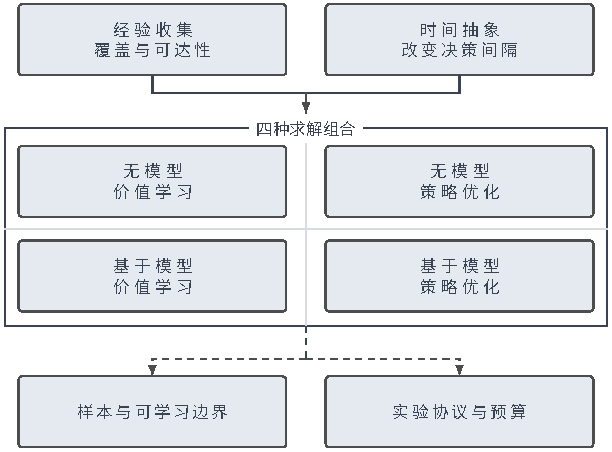
\includegraphics[width=103.618mm]{figures/10-reinforcement-learning/01-problems-and-solving/tikz/rl-learning-map.pdf}
  \caption{本章的问题关系。实线表示经验收集和时间抽象与四种求解接口之间的依赖或组合关系，虚线表示统一的分析与评价口径；四种求解接口没有先后执行关系。}
  \label{fig:rl-learning-map}
\end{figure}

% Outline: 3.1
\section{支持策略改进的经验收集}
\label{sec:rl-learning-experience}

在网格中，如果当前策略总是绕开某条岔路，后续训练就永远不会得到那条岔路的转移和奖励——你无法从一份从未记录过的经验中学习。于是交互采集与策略更新之间形成一个闭环：策略决定下一批能看到哪些经验，经验又决定下一次如何改进策略。这正是强化学习区别于普通监督学习的根本困难。探索方法的条件因此必须分别按几件事来确定：决策前能看到什么观测、奖励服从什么规律、最终要推荐的是哪个动作或策略，以及动作是否会改变后续状态。

% Outline: 3.1.1
\subsection{探索问题中的不确定性与变化维度}
\label{sec:rl-learning-uncertainty}

面对网格中的不确定性，首先要分清它来自两种不同的源头，因为补充样本能够减少哪一种不确定性，需要分别判断。从未走过的岔路使我们完全不了解转移规律，这种因已掌握的转移与奖励记录不足而产生的不确定，称为\term{认知不确定性}（epistemic uncertainty）：已采集的交互样本不足以确定转移或奖励规律，而补充相关样本有可能缩小这种无知，它原则上可以通过学习消除。另一种是即使把规律摸得很熟也无法消除的\term{偶然不确定性}（aleatoric uncertainty）：规律本身就允许多个随机结果，例如滑移概率即使精确已知为$0.8/0.1/0.1$，下一次究竟落在哪里仍无法预言，增加再多样本也不会让某次滑移变得确定。区分二者的现实意义在于：重走熟悉的岔路能帮助把概率估得更准，却不可能消除滑移本身。因此，一次罕见结果不足以证明模型仍不了解该处（可能只是已知随机性的一次实现），反过来，已熟悉区域的预测误差很低，也不能证明那些重要却没走过的岔路都已探索充分。

区分这两种不确定性后，还需要确定未知量和采样目标。只估计各动作的奖励均值，与学习依用户特征选动作的规则，需要明确不同的决策前观测字段及样本间共享的奖励结构；在线服务与最终只推荐一个动作，也允许不同的试验代价。表\ref{tab:rl-learning-exploration-settings}把这些变化分开，条件仍可组合，例如可见用户特征的同时，奖励由对手改变。进入MDP时新增的则是可达性：本次动作会改变下一状态的分布，从而改变后续能取得的观测与奖励，而不只是多看到一列特征。

\begin{table*}[t]
  \centering
  \small
  \begin{tabularx}{\linewidth}{>{\raggedright\arraybackslash}p{25mm} >{\raggedright\arraybackslash}X >{\raggedright\arraybackslash}X >{\raggedright\arraybackslash}X}
    \toprule
    改变的条件 & 决策前可见的状态或上下文 & 一次动作提供的样本 & 典型输出 \\
    \midrule
    动作回报未知 & 动作集合、过去选择与奖励 & 所选臂的奖励 & 在线动作序列 \\
    上下文出现 & 本轮特征与过去反馈 & 当前特征下所选动作的奖励 & 从特征到动作的策略 \\
    奖励由对手选择 & 历史，可能还有上下文 & 所选动作的当轮奖励 & 相对指定比较类的低遗憾序列 \\
    只关心部署动作 & 与随机老虎机相同 & 可按识别需要分配的奖励样本 & 一个推荐动作及置信陈述 \\
    动作影响状态 & 当前状态、历史反馈 & 奖励与后继状态 & 能到达并利用高价值区域的策略 \\
    \bottomrule
  \end{tabularx}
  \caption{探索设定的变化维度。表中每行突出一个变化，不表示这些条件互斥。}
  \label{tab:rl-learning-exploration-settings}
\end{table*}

\paragraph{探索要评价什么}
探索到底“值不值”，需要先明确用什么尺子衡量，因为不同阶段关心的损失并不相同。\term{累积遗憾}统计的是在整个学习（试验）期间，因为反复试错而比“每步都选最优”少获得的期望回报，它关心学习过程本身的代价；\term{简单遗憾}只看试验结束后最终推荐出去的那个动作，比最优动作的均值差多少；\term{最终策略损失}则比较输出策略与参照策略在指定初始分布下的整段回报差。这三种量所用的基准和取期望的对象都由具体任务确定，老虎机中的公式见式\eqref{eq:rl-learning-bandit-regret}与式\eqref{eq:rl-learning-simple-regret}。判断经验是否覆盖了决策所需，也必须落到这些具体对象上：目标策略可能经过的路线有没有机会被采到、关键动作是否试过足够多次、已有奖励或转移样本是否足以约束共享表示在相关特征方向上的预测。仅仅说样本“很多”或“很多样”，回答不了这些问题。

这些指标考察的时间窗和对象不同，因而很可能相互冲突。为了确认一个看起来略差的动作其实略差（而不是被噪声误导），算法往往必须多试它几次：这会在试验期间少拿奖励、增大累积遗憾，却能让最终推荐更少出错、减小简单遗憾。同理，访问大量与通往终点无关的状态，虽然让“访问过的状态种类”变多，却不一定能为关键岔路上的动作价值提供约束。判断一次探索的收益，应看新样本是否真的减少了目标决策的不确定性，而不能只看交互记录的数量或多样性。

% Outline: 3.1.2
\subsection{动作回报未知：随机老虎机中的探索}
\label{sec:rl-learning-bandits}

我们先把网格里的状态转移完全拿掉，得到一个最干净的探索问题：每一轮都面对同一组$K$个动作，动作只影响本轮奖励，不改变下一轮的处境。这就是老虎机的选臂问题，其中一只“臂”就对应一个可以反复试验的动作。剥离状态后，问题反而更聚焦：我们仍然只能看到自己选中的那个臂的结果，没选的臂一无所知。麻烦在于早期奖励可能偶然偏低；如果从此再不选这个臂，这份错误估计就永远没有被纠正的机会。因此探索的核心张力是：既要利用当前看起来最好的臂多拿奖励，又要为其他可能其实更好的臂保留试验机会。

衡量试验代价时，自然以“始终选择真实均值最高的臂”作为参照。每当选到一个均值较低的臂，就比最优选择少拿两者的均值差；把这一损失按该臂被访问的次数累加，就得到下面的累积伪遗憾。参照中的最大值要遍历全部$K$个臂，追求的是较高奖励。取期望时，要对算法随机性及奖励历史共同造成的选臂次数随机性平均：即使选臂规则不使用内部随机数，先前看到的随机奖励也会改变后续选择。每次选择的损失使用真实均值差，而不是两条实现奖励序列的逐次差，这正是“伪”遗憾中“伪”的含义。

\begin{definition}[有界随机老虎机]
  \label{def:rl-learning-stochastic-bandit}
  给定正整数$K,T$。臂$a\in\{1,\ldots,K\}$有固定奖励分布$\nu_a$，每次拉动得到一个取值于$[0,1]$的新样本；给定选臂前历史和当前动作$a$，下一奖励的条件分布仍为$\nu_a$。记均值$m_a$、最优均值$m_*=\max_a m_a$、差距$\Delta_a=m_*-m_a$，以及前$T$轮臂$a$的访问数$N_a(T)$。累积伪遗憾为
  \begin{equation}
    \mathcal R_T
    =T m_*-\mathbb E\!\left[\sum_{t=1}^T m_{a_t}\right]
    =\sum_{a=1}^K\Delta_a\,\mathbb E N_a(T).
    \label{eq:rl-learning-bandit-regret}
  \end{equation}
  “伪”表示比较的是均值，而不是两条独立随机奖励序列的逐次差。
\end{definition}

\begin{example}[一次噪声如何锁住贪心策略]
  \label{ex:rl-learning-greedy-trap}
  教学设定中，两臂分别为均值$0.7$和$0.4$的伯努利分布。各试一次，恰好观察到$(0,1)$的概率为$0.3\times0.4=0.12$。此后纯贪心不再试第一臂，而第二臂的经验均值在任意有限次采样后都严格为正，因为最初的那个1仍在样本中。因此第一臂的估计一直停在0，算法可以永久错选；这不是两个均值太接近，而是未被选择的臂失去了纠错机会。
\end{example}

\term{$\varepsilon$-贪心}用显式随机来打破上述闭环：以概率$1-\varepsilon_t$选择当前经验均值最高的臂（利用），以概率$\varepsilon_t$在所有臂中均匀随机地试一个（探索）。若采用固定的$\varepsilon_t\equiv\varepsilon>0$，每个臂都以至少$\varepsilon/K$的概率获得试验机会；存在正差距时，仅这部分固定比例探索就会使累积伪遗憾随轮数线性增长。逐轮为正却不等于固定比例：例如$\varepsilon_t=t^{-2}$的探索概率之和有限，不能保证每个臂都被无限探索。衰减过快可能使早期错误失去纠正机会，合适的衰减日程则还需结合奖励分布和臂间差距分析。均匀随机探索没有按“每个动作究竟还剩多少不确定性”来精细分配试验次数。

\term{置信上界}（upper confidence bound, UCB）的思路更聪明：与其盲目随机，不如给每个动作构造一个“按现有样本尚不能排除的较高可能均值”，用这个乐观值为动作评分。当两个臂经验均值相近时，样本少的那个估计更不可靠、可能的上限更高，于是值得再查一次；随着被抽次数增多，它的误差区间收窄，乐观加分自动下降。记轮$t$前的经验均值为$\widehat m_a(t)$、已抽次数为$N_a(t)$；未访问过的臂先各试一次，以免分母为0。UCB1随后在全部臂中选择“经验均值加上区间半宽”最大的动作：
\begin{equation}
  a_t\in\argmax_a\left\{\widehat m_a(t)
    +\sqrt{\frac{2\log t}{N_a(t)}}\right\}.
  \label{eq:rl-learning-ucb}
\end{equation}
均值高带来利用，区间宽带来探索。图\ref{fig:rl-learning-bandit-geometry}左侧的教学快照把半宽简化为$(0.05,0.20,0.12)$，三个均值估计为$(0.55,0.48,0.30)$，因此上界分别为$(0.60,0.68,0.42)$。第二臂的当前均值不是最高，却最值得再查一次；这些示意半宽只是教学设定，并非将某个指定时刻的奖励采样记录代入式\eqref{eq:rl-learning-ucb}计算而来。

置信区间刻画的是“未知均值可能落在什么范围”，而不是“下一次奖励会落在哪里”，这一点务必分清。即使某个伯努利臂的均值已被精确确定为$0.7$，下一次奖励仍然只可能是0或1；置信区间不会因此变宽或变窄。半宽随$N_a^{-1/2}$缩小，反映重复采样使均值估计越来越精确；分子中缓慢增长的$\log t$则保证即使到了后期，也仍为各臂保留一点点重新检视的误差余量。按区间上端点行动，含义是“暂时假定该臂仍可能有这么好，于是再给它一次试验机会”，而不是断言它的真实均值就等于这个乐观上端点。

除了用区间表达不确定性，还可以直接为“均值可能取哪些值”维护一份概率分布：抽样前对未知均值的初始判断称为先验，观察到奖励后，按“先验乘以该奖励在各均值下出现的概率”再归一化，得到后验。后验描述的是我们对未知均值的相信程度，仍然不是下一次奖励本身的分布。\term{Thompson采样}（Thompson sampling）的做法是：每一轮先从这份后验中随机抽出一组“假设的均值”，把它当作本轮暂时为真的环境，再选其中最大的臂。这样一来，那些尚不确定、但有不小概率其实最优的臂，自然会获得试验机会，而无须显式计算区间。若联合后验因子化，例如各臂先验独立且奖励似然按臂分解，就可以逐臂独立抽样；存在后验相关性时，须保留它。固定以编号最小者打破并列，规则可以写为
\[
  \widetilde{\bm m}_t\sim p(\mathrm d\bm m\mid I_t),
  \qquad a_t=\min\argmax_a\widetilde m_{t,a},
\]
其中$I_t$为本轮选臂前已取得的动作与奖励记录。抽样向量与未知均值向量具有同一后验分布，所以
\[
  \mathbb P(a_t=a\mid I_t)
   =\mathbb P\!\left(a=\min\argmax_b m_b\mid I_t\right).
\]
因此，概率匹配针对的是按同一并列规则选出的最优臂事件；没有并列时，它就是该臂为唯一最优臂的后验概率。

例如伯努利奖励配$\operatorname{Beta}(1,1)$先验，观察$(1,0,1)$后，似然$m^2(1-m)$使该臂后验变为$\operatorname{Beta}(3,2)$，后验均值为$3/5$；但选臂用的是本轮抽样值，不是这个均值。若三个抽样值为$(0.58,0.63,0.27)$，就选第二臂。这一解释依赖给定的先验和奖励模型；后验可信区间是否具有频率学覆盖率，仍需另行分析。

\begin{example}[独立抽取边缘后验会改变选臂概率]
  \label{ex:rl-learning-thompson-joint}
  设两臂均值的联合后验以各$1/2$的概率取$(0.2,0.1)$或$(0.4,0.3)$。两种情况下第一臂都更好，正确的联合抽样因此总选第一臂。如果分别从两个边缘后验独立抽样，就会以$1/4$的概率拼出$(0.2,0.3)$并误选第二臂。这组均值在原联合后验下根本不会出现；差别来自抽样时丢掉了相关性。
\end{example}

UCB1的一个经典结果能说明探索成本怎样进入式\eqref{eq:rl-learning-bandit-regret}。在上述固定、独立、有界奖励条件下，对每个$\Delta_a>0$的臂，
\begin{equation}
  \mathbb E N_a(T)
  \leq \frac{8\log T}{\Delta_a^2}+1+\frac{\pi^2}{3},
  \qquad
  \mathcal R_T
  \leq\sum_{a:\Delta_a>0}
    \left(\frac{8\log T}{\Delta_a}
    +\left(1+\frac{\pi^2}{3}\right)\Delta_a\right).
  \label{eq:rl-learning-ucb-bound}
\end{equation}
这里$\pi$在常数$\pi^2/3$中是圆周率，不是策略。证明的关键不是直接控制所有动作选择，而是控制错误选择所需的事件：若最优臂没有被低估、次优臂没有被高估，而且次优臂已访问超过$8\log T/\Delta_a^2$次，它的置信上界就不能超过最优臂。对预先固定样本数$n$，独立同分布的$[0,1]$奖励均值满足$\mathbb P(|\widehat m_n-m|>u)\leq2e^{-2nu^2}$，$u>0$；对全部可能访问数和轮次分配失败概率，再用联合界限制前两类坏事件；对可能的样本数和轮次求和得到常数项；剩余访问数乘差距便得到遗憾。自适应选臂要求同时控制各个可能的样本数，不能只在最终随机访问数上直接套一次固定样本不等式。上述常数和算法来自UCB1原始分析\scite{rl3-auer2002finite}这里使用的是有界独立奖励的集中界，不是把自适应产生的整条奖励序列当成独立样本。条件期望、换测度、集中与鞅工具可参考\BookChapterRef{chap:random-sequences-and-processes}{卷2《数学准备：概率、因果与决策》的“随机序列与随机过程”章}；应用到TD、离策略估计和线性置信椭球时，仍须分别核对条件矩、支持和可预测性。

对数代价也有统计辨识的解释。两个奖励分布可能具有接近的均值，但我们实际用来辨认它们的是随机样本。对某个观察结果，比较它在两种分布下的概率，便得到似然比；连续多个独立样本的比率相乘，取对数后证据相加。将单次对数比在当前分布下平均，得到\term{KL散度}（Kullback--Leibler divergence），用于衡量一个样本平均提供多少分布辨识证据。令$\mu$为当前臂的奖励分布、$\nu$为同一奖励空间上的替代分布。若$\mu\ll\nu$，即$\nu$不可能的事件在$\mu$下也不可能，平均对数似然证据为
\[
 D_{\mathrm{KL}}(\mu\Vert\nu)
   =\mathbb E_{r\sim\mu}\log\frac{\mathrm d\mu}{\mathrm d\nu}(r).
\]
这里采用自然对数，单位为nat；离散奖励时是$\sum_r\mu(r)\log[\mu(r)/\nu(r)]$，零质量项取0。若$\mu$给某事件正质量而$\nu$给它零质量，散度为$+\infty$；即使绝对连续，散度也未必有限。方向由当前分布下的期望确定，不能交换。后面的奖励辨识下界、策略KL约束与技能目标都要保留这个分布比较对象。KL、互信息及局部分布几何可参考\BookChapterRef{chap:information-theory-and-statistical-geometry}{卷2《数学准备：概率、因果与决策》的“概率分布的分析与优化”章}。

Lai--Robbins分析考虑满足正则条件的参数化奖励族与一致有效策略，即在该族每个实例上，对任意$c>0$都有$\mathcal R_T=o(T^c)$。若一个次优臂的分布改成均值超过$m_*$的合法分布，算法必须收集足够样本区分这两个世界；所需次数满足渐近下界
\[
  \liminf_{T\to\infty}\frac{\mathbb E N_a(T)}{\log T}
  \geq
  \frac{1}{\inf_{\nu:\,\mathbb E_\nu r>m_*}
                D_{\mathrm{KL}}(\nu_a\Vert\nu)}.
\]
分母中的候选$\nu$只取所声明奖励族内、均值超过$m_*$的合法分布；下确界选出与当前次优臂最难区分的替代分布。KL越小，仅凭一个奖励样本越难区分两种奖励分布，算法就越需要重复试验。伯努利分布只需比较成功和失败两种结果；记
\[
  \operatorname{kl}(p,q)
    :=D_{\mathrm{KL}}(\operatorname{Ber}(p)\Vert\operatorname{Ber}(q))
    =p\log\frac pq+(1-p)\log\frac{1-p}{1-q}.
\]
对$0<p,q<1$可直接使用上式，端点按前述零质量和零支持约定处理。若$0<m_a<m_*<1$，伯努利族中的替代均值从$m_*$上方趋近，分母的下确界为$\operatorname{kl}(m_a,m_*)$。这是固定分布族内、依赖当前实例的渐近辨识成本，不是任意非平稳奖励下都存在的$\log T$保证\scite{rl3-lai1985adaptive}

% Outline: 3.1.3
\subsection{反馈条件变化：上下文与对抗老虎机}
\label{sec:rl-learning-contextual}

同一个推荐动作，对不同的用户（或不同情境）可能产生完全不同的奖励。如果决策前已经能看到刻画当前情境的特征，却仍为每个动作只存一个不分对象的全局均值，就等于忽略了当前用户或情境特征对奖励的影响。\term{上下文老虎机}（contextual bandit）学习的正是一条根据本轮可见特征选择动作的规则；这里的“上下文”就是动作选择之前就能看到的特征。它与MDP的关键简化是：假定动作不改变下一轮上下文的生成机制（当前推荐不会改变明天来的是什么用户），从而可以把“依据特征预测条件奖励”的问题与MDP中“动作改变后续状态”的纠缠分开来单独研究。

为了让不同用户和动作共享样本，先假定奖励均值是已知特征的线性函数。动作$a$在轮$t$的特征为$\bm{x}_{t,a}\in\mathbb R^d$，未知系数为$\bm\theta_*$。下面第一式规定奖励与噪声的关系，后两式用过去实际选中的特征和奖励计算正则化最小二乘估计：
\begin{equation}
  r_t=\bm{x}_{t,a_t}^{\top}\bm{\theta}_*+\eta_t,\qquad
  \bm{V}_t=\lambda\bm{I}+\sum_{u<t}\bm{x}_{u,a_u}\bm{x}_{u,a_u}^{\top},
  \quad
  \widehat{\bm{\theta}}_t
  =\bm{V}_t^{-1}\sum_{u<t}\bm{x}_{u,a_u}r_u .
  \label{eq:rl-learning-linear-bandit}
\end{equation}
假设特征在选动作前已知、$\lVert\bm{x}_{t,a}\rVert_2\leq L$、$\lVert\bm{\theta}_*\rVert_2\leq B_{\theta}$，噪声相对于历史条件均值为0且为$R$-次高斯，正则化$\lambda>0$。这些条件容许自适应选择特征，但不容许噪声在看到本轮抽样结果后任意配合奖励。

式\eqref{eq:rl-learning-linear-bandit}来自一个回归问题：用$\bm x_{u,a_u}^{\top}\bm\theta$预测已观察的$r_u$，最小化过去平方残差之和，再加$\lambda\|\bm\theta\|_2^2$限制参数大小。求导并令其为0，得到$\bm V_t\widehat{\bm\theta}_t=\sum_{u<t}\bm x_{u,a_u}r_u$。因此$\bm V_t$既用于求参数，也记录哪些特征方向已被样本约束；$\lambda\bm I$保证样本尚少时矩阵仍可逆。这里的次高斯条件约束噪声尾部：对任意实数$v$，有$\mathbb E[e^{v\eta_t}\mid I_t,a_t]\leq e^{R^2v^2/2}$，其中$I_t$为动作前历史。它用于控制估计误差，不要求噪声恰好为高斯分布。

选臂需要知道这份参数估计在当前动作方向上还能错多少，而不只是各坐标的误差。自归一化集中将参数误差与自适应采样得到的$\bm V_t$一起控制，给出形如$\lVert\widehat{\bm{\theta}}_t-\bm{\theta}_*\rVert_{\bm{V}_t}\leq b_t^{\mathrm{conf}}$的高概率椭球，其中$\lVert\bm{z}\rVert_{\bm{V}}^2=\bm{z}^{\top}\bm{V}\bm{z}$。对允许失败概率$\delta\in(0,1)$，一个常用半径是
\[
  b_t^{\mathrm{conf}}=R\sqrt{2\log
       \frac{\det(\bm{V}_t)^{1/2}}
            {\det(\lambda\bm{I})^{1/2}\delta}}
       +\sqrt{\lambda}B_{\theta} .
\]
在适用的时间一致事件上，这个椭球同时限制各轮参数误差。对某个已知动作特征，我们在椭球内选择预测奖励最高的参数，得到该动作的乐观评分；最大化的对象是尚未被已见奖励样本排除的参数，而不是任意实向量。利用柯西不等式可得
\[
  \max_{\lVert\bm{\theta}-\widehat{\bm{\theta}}_t\rVert_{\bm{V}_t}\leq b_t^{\mathrm{conf}}}
  \bm{x}_{t,a}^{\top}\bm{\theta}
  =
  \bm{x}_{t,a}^{\top}\widehat{\bm{\theta}}_t
  +b_t^{\mathrm{conf}}\sqrt{\bm{x}_{t,a}^{\top}\bm{V}_t^{-1}\bm{x}_{t,a}}.
\]
若$\bm{V}_t=\operatorname{diag}(4,100)$，沿两个坐标方向的不确定半宽分别为$0.5b_t^{\mathrm{conf}}$和$0.1b_t^{\mathrm{conf}}$。多次观察第二个方向不会自动了解与之正交的第一个方向。图\ref{fig:rl-learning-bandit-geometry}右侧示意这种长轴沿特征样本约束较弱的方向展开的关系，轴长不按该数例的比例绘制。

\begin{figure*}[t]
  \centering
  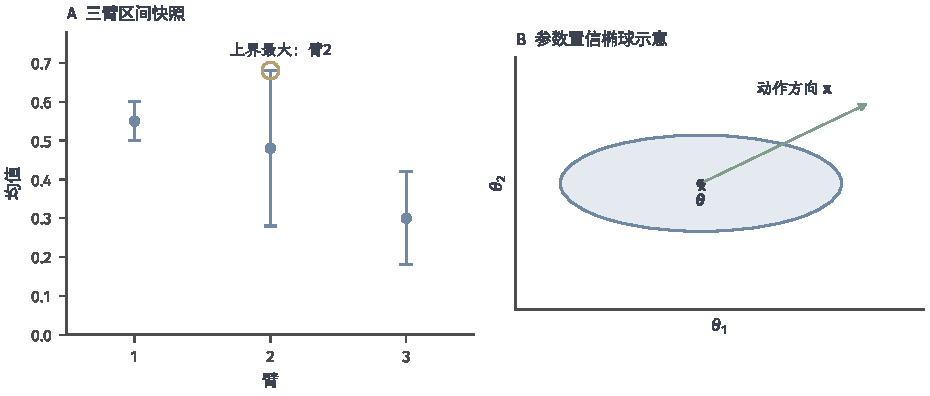
\includegraphics[width=157.400mm]{figures/10-reinforcement-learning/01-problems-and-solving/matplotlib/rl-learning-bandit-geometry.pdf}
  \caption{动作区间与参数椭球。左图为明确标注的三臂教学快照，UCB选择上端点最大的第二臂；右图示意线性参数置信集合，较长的轴对应奖励样本约束较弱的参数方向。二者都把不确定性转成动作评分，但线性模型还通过共享特征把奖励样本的约束扩展到其他动作。}
  \label{fig:rl-learning-bandit-geometry}
\end{figure*}

\Needspace{14\baselineskip}
LinUCB常以这个方向性奖励构造动作评分；OFUL直接在联合参数置信集合中做乐观选择，并把集合有效性纳入分析\scite{rl3-abbasi2011linear}
线性Thompson采样则抽取整个参数向量，再对所有动作用同一个抽样参数评分。共享的是线性结构和设计矩阵，而不是“把标量UCB换成更大网络”就能保留的保证。具体统计结论依赖所用噪声模型、置信半径或抽样尺度。

若奖励规律不固定，每个臂可能根本没有待估计的固定均值。我们改用无上下文的对抗老虎机：对手在本轮实际抽样前选择奖励向量$\bm{r}_t\in[0,1]^K$，智能体只看到$r_{t,a_t}$。对手可依赖过去历史，却不能在看到本轮动作后临时改写奖励。此时EXP3用权重记录各臂迄今的奖励证据，并把权重归一化成抽样概率。为更新未被选臂也有定义的奖励估计，所选臂的奖励除以其抽样概率，其他臂记0；下面三式依次给出抽样、估计与指数权重更新：
\begin{equation}
  p_{t,a}=(1-\varepsilon)\frac{w_{t,a}}{\sum_b w_{t,b}}
                 +\frac{\varepsilon}{K},\quad
  \widehat r_{t,a}=\frac{\mathbf 1\{a_t=a\}r_{t,a_t}}{p_{t,a}},
  \quad
  w_{t+1,a}=w_{t,a}\exp(\eta\widehat r_{t,a})
  \label{eq:rl-learning-exp3}
\end{equation}
估计奖励较高的臂获得更大的下一轮权重。各臂权重从正值开始；$0<\varepsilon\leq1$保证所有抽样概率为正，$\eta$与$\varepsilon$必须按具体遗憾分析配合，而不能任意取大值。

逆概率加权的意义可以先用一个数看清。固定某轮奖励为$0.6$的臂，若它以概率$0.2$被选中，就在选中时记$0.6/0.2=3$，其余时候记0。平均为$0.2\times3=0.6$，恰好恢复该臂本轮奖励。这个估计数可以超过奖励上限1，因为它承担的是补偿少抽样的权重，不是模拟一次真实奖励。抽样概率越小，偶尔出现的加权值越大，有限样本波动也越强。

无偏性的条件可以直接检查。固定抽样前历史及本轮奖励向量后，
\[
  \mathbb E[\widehat r_{t,a}\mid\text{历史},\bm{r}_t]
  =p_{t,a}\frac{r_{t,a}}{p_{t,a}}=r_{t,a}.
\]
概率小会放大方差，但不会在这些条件下改变条件均值。若对手看到$a_t$后才选择$\bm{r}_t$，这一步条件化便不成立。通常的外部遗憾比较事后最佳固定臂，而不是每轮都预知奖励的全知动作序列；对抗上下文算法还要明确比较的策略类。EXP3的原始保证正是围绕这种反馈与比较协议建立的\scite{rl3-auer2002nonstochastic}

% Outline: 3.1.4
\subsection{学习目标变化：累积遗憾与最佳臂识别}
\label{sec:rl-learning-best-arm}

同样的随机老虎机，若试验期间也要服务用户，就需要控制累积收益损失；若只在试验后部署一个动作，则可以多试当前看来略差的候选，换取更可靠的推荐。后一种任务称为最佳臂识别，评价的是输出而非整段动作序列。预算结束时输出$\widehat a_T$，下面分别计算它比最佳均值差多少，以及它落在最优臂集合之外的概率；两者都越小越好：
\begin{equation}
  \mathfrak r_T=\mathbb E[m_*-m_{\widehat a_T}],
  \qquad
  \mathbb P\{\widehat a_T\notin\argmax_a m_a\}.
  \label{eq:rl-learning-simple-regret}
\end{equation}
错选一个只差$10^{-4}$的动作，对这两个指标的影响并不相同。仅报告推荐错误率会把近乎无损与严重失误放在同一类别中。表\ref{tab:rl-learning-identification-protocols}进一步区分何时结束试验：预算耗尽与证据充分，是两种不同的停止依据。

\begin{table}[htbp]
  \centering
  \small
  \begin{tabularx}{\linewidth}{>{\raggedright\arraybackslash}p{22mm} >{\raggedright\arraybackslash}X >{\raggedright\arraybackslash}X}
    \toprule
    协议 & 预先固定什么 & 算法输出与待分析量 \\
    \midrule
    固定预算 & 总拉臂次数$T$ & 推荐$\widehat a_T$；分析简单遗憾或错误概率 \\
    固定置信度 & 允许错误$\delta$，必要时精度$\epsilon$ & 随机停止时间$\tau$和推荐$\widehat a_\tau$；保证错误概率不超过$\delta$并分析$\mathbb E\tau$ \\
    \bottomrule
  \end{tabularx}
  \caption{纯探索的两种协议。固定置信度不是先任意选择预算，再宣称置信度已经满足。}
  \label{tab:rl-learning-identification-protocols}
\end{table}

固定置信度协议允许边采样边检查是否停止，因而停止时的样本数由已见奖励记录决定。只在某个预先固定样本数有效的区间不足以支持这种反复查看。我们给全部臂、全部正整数样本数同时分配失覆盖概率；对$[0,1]$奖励，取下面的半宽与区间：
\[
  \begin{aligned}
    c(n)&=\sqrt{\frac{\log(2K n(n+1)/\delta)}{2n}},\\
    [L_a(n),U_a(n)]&=[\widehat m_a(n)-c(n),\widehat m_a(n)+c(n)].
  \end{aligned}
\]
Hoeffding不等式给出单个$(a,n)$的失覆盖概率不超过$\delta/[K n(n+1)]$。因为$\sum_{n\geq1}1/[n(n+1)]=1$，联合界保证全部臂、全部样本数同时覆盖的概率至少为$1-\delta$。这不是最紧的边界，却明确处理了自适应停止。

\term{逐次淘汰}（successive elimination）保留尚可能最优的臂；若$U_a<\max_b L_b$，则淘汰$a$。在全部区间覆盖的事件上，真正最优臂不可能满足淘汰条件。教学快照若三个区间为$[0.55,0.65]$、$[0.40,0.52]$、$[0.42,0.70]$，第二臂可淘汰，第一、第三臂还不能分胜负。LUCB把试验集中到当前经验最优臂$b$与其余臂中上界最大的竞争者$c$\scite{rl3-kalyanakrishnan2012pac}
当$L_b\geq U_c-\epsilon$时，可以推荐一个$\epsilon$-最优臂。这个例子中下一步重点采第一和第三臂，而不是轮流采已排除的第二臂。

区间正确时，淘汰和停止逻辑便给出正确性；样本复杂度还要分析何时区间足够窄。固定置信度理论进一步研究不同臂之间的最优样本分配\scite{rl3-kaufmann2016complexity}
从区间宽度看，为了分开差距$\Delta_a$，半宽通常要降到$\Delta_a$的常数比例，所需样本因而带有$\Delta_a^{-2}$量级和置信度对数项，但这一粗略尺度不能给出最优常数。差距趋近0会使精确识别越来越昂贵；并列最优时，要求用严格区间分离证明唯一最优可能永不停止，应改用适合并列情形的识别目标，例如允许正精度的$\epsilon$-最优识别。

% Outline: 3.1.5
\subsection{状态随动作变化：MDP中的覆盖、可达性与长时程探索}
\label{sec:rl-learning-deep-exploration}

回到MDP，每轮并不会自动把智能体送回同一组候选动作面前。某扇门只有到达门口才能尝试，一次转向可能让后续奖励区域暂时不可达。图\ref{fig:rl-learning-exploration-chain}左侧是由网格导航抽出的独立教学链：取消滑移，增设单向门与失败后重置，连续$H$次必要选择才能到达唯一奖励。若每次独立均匀试两个动作，一回合走完全链的概率为$2^{-H}$；这个数字描述该随机试验方案，不是所有能观察状态的算法都必须付出的下界。

\begin{figure*}[t]
  \centering
  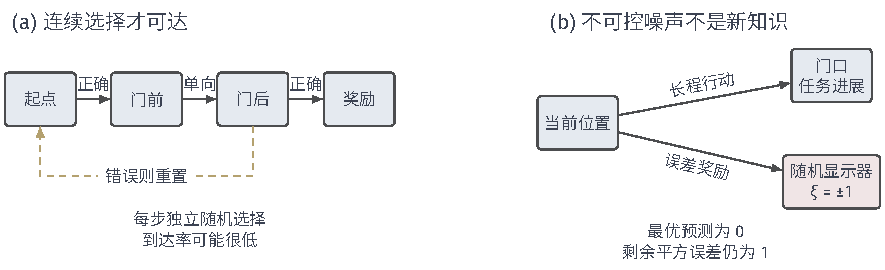
\includegraphics[width=149.818mm]{figures/10-reinforcement-learning/01-problems-and-solving/tikz/rl-learning-exploration-chain.pdf}
  \caption{可达性与预测误差的两个教学反例。左侧为从导航任务抽出的确定性单向门链，每一步错误都会重置；右侧的随机显示器可持续制造不可控预测误差，却不帮助通过门口。两者均为明确修改过的独立任务，不是基准网格的新转移规则。}
  \label{fig:rl-learning-exploration-chain}
\end{figure*}

在这条链上，“试一下最后一道门”首先要求走过前面的门。已经确认的前缀应被后续探索保留，新的随机选择集中在尚不了解的部分。这样的长时程探索将一次试验看成持续多步的行为：当前动作不仅为了本步奖励，也为了取得较远处的证据。下面的乐观备份和整回合后验采样，分别用价值传播和一致的模型假设维持这种方向。

要探索链末端，当前动作必须能利用对远处尚未确定收益的估计。乐观价值先给未充分访问的状态动作较高估值，再通过Bellman备份将它传向上游；模型置信集合则保留尚未被已见转移与奖励记录排除的转移核与奖励规律，选其中预计回报较高的模型来规划。后验采样强化学习（posterior sampling for reinforcement learning, PSRL）在回合开始抽取一套完整动力学和奖励，再在整回合执行其策略。这样多个时刻共享同一个探索假设，不会像逐步重新随机选方向那样频繁放弃当前路线。后验及其计算仍依赖模型假设，有限样本表格保证将在第\ref{sec:rl-learning-statistical-limits}节另列条件\scite{rl3-osband2013posterior}

也可以不显式规划一个乐观模型，而在训练奖励中加入鼓励访问未充分采样状态动作的内部信号。这称为内在奖励（intrinsic reward）：外在任务奖励仍为$r_t$，训练使用$r_t+\eta_{\mathrm{int}} b_t$，其中$b_t$由采样或预测记录构造，$\eta_{\mathrm{int}}$决定探索信号的权重。表\ref{tab:rl-learning-intrinsic}比较不同$b_t$的测量对象。加入它会改变训练时的选择偏好，所以评价必须另报不含内在奖励的任务回报，才能确认探索最终帮助了原任务。

用预测误差产生内在奖励时，需要先明确“预测什么”。ICM（intrinsic curiosity module，内在好奇心模块）用当前与后继特征反推已执行动作，借此训练表示，再预测给定动作后的特征；预测错的部分产生内部奖励。RND（random network distillation，随机网络蒸馏）则固定一个随机初始化的网络，用另一个网络模仿它对当前观测的输出。观测越少参与拟合，输出差可能越大；固定目标网络并不是在预测真实环境。两者都把某种拟合误差转为探索信号，是否测到可减少的无知，还要检查噪声和表示。

\begin{table*}[t]
  \centering
  \small
  \begin{tabularx}{\linewidth}{>{\raggedright\arraybackslash}p{24mm} >{\raggedright\arraybackslash}X >{\raggedright\arraybackslash}X}
    \toprule
    方法 & 估计对象与典型信号 & 怎样改变行为及主要边界 \\
    \midrule
    访问计数 & $b_t(s,a)=1/\sqrt{N_t(s,a)+1}$ & 奖励少访问位置；离散计数需要有意义的状态划分 \\
    伪计数 & 用密度模型更新前后的概率变化构造计数替代 & 将新颖性扩到大状态空间；依赖密度学习假设，不是实际访问次数 \\
    ICM & 学习特征中的动作条件前向预测误差，配合逆动力学表示 & 偏向可由动作影响的特征；不能保证剔除所有噪声 \\
    RND & 可训练预测器与固定随机目标网络的输出差 & 以拟合困难代表新颖性；泛化、遗忘和观测噪声会影响分数 \\
    回合内好奇心 & 当前嵌入与本回合记忆的距离或近邻密度 & 鼓励回合内未访区域；跨回合重置记忆改变了“新”的含义 \\
    \bottomrule
  \end{tabularx}
  \caption{新颖性信号的计算对象。表中的奖励是训练工具，不自动对应环境转移的置信区间。}
  \label{tab:rl-learning-intrinsic}
\end{table*}

按表中的计数公式，同一教学状态的两个动作已访问99次和3次，探索奖励分别为$0.1$和$0.5$；后者因样本更少而得到更高偏好。预测误差却可能在观测样本充分后仍然很大。设与位置无关的显示器每步独立输出$\xi_t\in\{-1,1\}$，两值等概率。平方损失下最优预测为0，剩余期望误差仍是$\mathbb E\xi_t^2=1$。把这项误差奖励给智能体，可能使它停在显示器旁：它已经知道显示规律，却仍能持续获取探索奖励。这就是noisy-TV反例，说明不可预测性不能直接当成可通过采样减少的无知。

\Needspace{16\baselineskip}
ICM在学习到的特征空间预测动作后果，用预测误差提供探索信号；表示的学习目标影响哪些变化会被当成值得探索的后果\scite{rl3-pathak2017curiosity}

\Needspace{16\baselineskip}
RND改为预测固定随机网络的输出，避免直接用随机后继的不可预测性作为目标；但其新颖性仍依赖观测表示、预测器训练及其训练观测样本的分布\scite{rl3-burda2019rnd}
ICM、RND与回合记忆分别改变表示、预测目标或比较范围，缓解条件并不相同。

在特别稀疏的任务中，还要区分“发现过某个状态”与“能稳定再到达它”。Go-Explore保存已发现状态及其到达路径，返回选定状态后继续探索，再处理带执行随机性的稳健复现。模拟器存档恢复提供了普通单轨迹交互没有的访问能力；即使两者都记录一百万步，允许采集的状态动作与重置条件也不同。探索性课程可以从更易到达的起点或子目标逐步扩展，但必须说明谁提供重置和任务选择。目标重标记如何把失败轨迹变成其他任务的成功经验，留到第\ref{chap:rl-transfer}章讨论\scite{rl3-ecoffet2021goexplore}

若勘查时还不知道将来要送往哪一个区域，探索目标就不能只围绕当前任务奖励。奖励无关探索先收集转移记录，奖励函数在采集结束后才给出，要求不再交互也能为它规划。此时重要的是记录能否支持全部允许奖励下的决策，而非已有技能是否容易区分；具体协议与统一保证见第\ref{sec:rl-learning-guarantees-access}节。

% Outline: 3.2
\section{无模型的价值学习}
\label{sec:rl-learning-value}

取得经验后，还需把观察到的奖励和后继变成长期价值估计。第\ref{chap:rl-planning}章的Bellman备份计算条件期望；现在只能用样本逼近它。固定产生目标回报的策略后，完整回报与自举目标具有不同的采样和估计误差；根据价值进一步改变行为或共享函数参数，又会引入评价与改进的耦合。

% Outline: 3.2.1
\subsection{完整回报与一步自举}
\label{sec:rl-learning-mc-td}

一条到达终点的轨迹已记录沿途全部奖励，我们可以把某次访问之后的奖励折扣相加，作为该状态的一次价值样本。\term{蒙特卡罗}（Monte Carlo, MC）评价就用这种完整随机回报修正估值：样本回报高于当前预测时上调，低于预测时下调。设回合在$T$终止，$V(s_T)=0$，目标及更新为
\begin{equation}
  G_t=\sum_{j=0}^{T-t-1}\gamma^j r_{t+j},
  \qquad
  V(s_t)\leftarrow V(s_t)+\alpha_t[G_t-V(s_t)].
  \label{eq:rl-learning-mc}
\end{equation}
更新中的$\alpha_t$是步长，控制这次样本占多大权重。把第二式写成$(1-\alpha_t)V(s_t)+\alpha_tG_t$，就能看出它在旧估计与新回报之间加权。若某状态已有$n-1$个选定回报样本的均值，第$n$个样本到来时取$\alpha=1/n$，更新后恰为$n$个样本的均值。因此这条递推首先是一种不必保存全部旧回报的平均算法；其他步长则采用不同加权，不能都解释成普通样本均值。

首次访问MC对每回合第一次出现的状态更新，每次访问MC对该状态的所有出现都更新。二者利用的回报都来自真实奖励，但同一回合内重复访问对应的回报并不独立。

若回合很长，等待完整回报会推迟更新；继续任务甚至没有自然的回合终点。Bellman关系提供了另一种目标：把已观察的一步奖励与下一状态的当前估值相加。\term{时序差分}（temporal difference, TD）用这个目标与当前预测的差立即更新，$\delta_t$就是这次样本的预测差：
\begin{equation}
  \delta_t=r_t+\gamma V(s_{t+1})-V(s_t),\qquad
  V(s_t)\leftarrow V(s_t)+\alpha_t\delta_t .
  \label{eq:rl-learning-td-zero}
\end{equation}
这种用已有预测构造新目标的做法称为\term{自举}（bootstrapping）。终止转移的下一价值是0；继续任务的人工时间截断则不能一概置0。表\ref{tab:rl-learning-mc-td}把目标的偏差来源与更新时机分开，避免把一步目标尚不准确误解为最终估计必然有偏。

\begin{example}[同一终止轨迹上的不同目标]
  \label{ex:rl-learning-mc-td}
  在基准随机网格中，一条可能的轨迹依次经过
  \[
    (1,1),(1,1),(2,1),(3,1),(4,1),(4,2),(4,3).
  \]
  第一次向右时向下滑移撞墙，因此留在原位；其后五步实现意图方向。奖励为五个$-0.04$和末步的1。于是起点两次访问的回报分别为
  \[
    \begin{aligned}
      G_0&=-0.04\frac{1-0.9^5}{1-0.9}+0.9^5=0.426686,\\
      G_1&=-0.04\frac{1-0.9^4}{1-0.9}+0.9^4=0.51854.
    \end{aligned}
  \]
  只看这一回合，首次访问样本是$0.426686$，每次访问的样本平均为$0.472613$。它们都是该轨迹产生的估计，不是起点的精确策略价值。若冻结估值$V(1,1)=0.2$、$V(2,1)=0.3$，前两次TD目标却分别是$-0.04+0.9(0.2)=0.14$和$-0.04+0.9(0.3)=0.23$。取步长$0.5$，第一条TD更新把起点估值从$0.2$改为$0.17$；从相同初值做首次访问MC则得到$0.313343$。这里为了比较目标没有把各方法串行混用。
\end{example}

\begin{table}[htbp]
  \centering
  \small
  \begin{tabularx}{\linewidth}{>{\raggedright\arraybackslash}p{22mm} >{\raggedright\arraybackslash}X >{\raggedright\arraybackslash}X}
    \toprule
    比较对象 & MC & TD(0) \\
    \midrule
    更新何时可得 & 等实际回报完成 & 观察一步转移即可 \\
    随机性来源 & 之后整段奖励和状态 & 当步奖励、后继状态及当前估值 \\
    对初值的依赖 & 初值不进入回报目标 & 后继估值进入目标 \\
    目标的条件均值 & 固定策略完整回报对应$V^\pi$ & 对应$\mathcal B^\pi V$，通常不等于$V^\pi$ \\
    适用注意 & 需终止或处理无限回报尾项 & 需控制自举与采样条件 \\
    \bottomrule
  \end{tabularx}
  \caption{目标偏差不等于最终估计偏差。TD目标含当前估值，不妨碍满足条件的表格迭代最终收敛到真实价值。}
  \label{tab:rl-learning-mc-td}
\end{table}

MC以已实现的整段回报作为目标，TD则把未来分成“刚看到的一步”和“尚未看到的其余部分”。后一部分由$V(s_{t+1})$暂时代替，所以目标会随价值估计一起改变。若后继估值过高，当前状态也可能被上调；若后继估值逐渐纠正，误差又会沿访问过程传回来。TD(0)中的0表示这里不使用跨步资格迹，资格迹将在下一小节解释。

随机的一步目标不必每次都更接近真实价值。固定当前估值$V$，对从状态$s$出发按$\pi$得到的许多一步样本平均，平均目标才是前章的$(\mathcal B^\pi V)(s)$。这里$\mathcal B^\pi$仍表示“即时奖励均值加折扣后继价值均值”。TD要用带噪声的更新追踪这项平均备份，直至备份前后相同；这与拿一个已知的正确标签做回归不同。

固定策略时，对给定$s_t=s$的动作、奖励和后继取平均，TD误差的条件均值为$(\mathcal B^\pi V)(s)-V(s)$。因此，样本更新虽然有噪声，平均方向仍指向Bellman不动点。在有限折扣MDP中，若奖励二阶矩受控、策略固定、每个需要评价的状态被无限访问，且各状态的访问步长满足$\sum_n\alpha_n(s)=\infty$、$\sum_n\alpha_n(s)^2<\infty$，配合相应马尔可夫噪声条件，可用随机逼近证明表格TD收敛。步长和发散使初始误差有机会被持续修正，平方和收敛则限制噪声的长期影响；Bellman压缩性确定唯一平衡点。这不覆盖任意常数步长或任意函数逼近。

MC的一致性则直接来自回报平均：独立回合的首次访问回报可用大数定律，每次访问版本要处理回合内依赖和访问次数的随机性。无限时域折扣MC若只截取有限长度，还留下尾项偏差。MC与TD都依赖轨迹采集和抽样条件，但依赖的方式不同\scite{sutton2018}

% Outline: 3.2.2
\subsection{多步回报、资格迹与时间信用}
\label{sec:rl-learning-traces}

MC一直使用真实奖励直到终点，TD(0)在一步之后就接入预测。若奖励需要多步才能传回当前状态，可以先观察$n$步奖励，再用第$n$步的估值补上余下未来。对固定估值$V$和终止时刻$T$，令$m=T-t$，允许长度$1\leq n\leq m$，得到
\begin{equation}
  G_t^{[n]}=\sum_{j=0}^{n-1}\gamma^j r_{t+j}
                    +\gamma^n V(s_{t+n}),\qquad V(s_T)=0.
  \label{eq:rl-learning-n-step}
\end{equation}
方括号$[n]$表示目标长度，不是参数迭代。$n$增大让奖励影响更快传过多步，但也把更多未来随机性带入一次目标。

先作一个独立的三步终止算例，观察目标长度改变了哪一部分。设奖励依次为$0,0,1$，$\gamma=0.9$，当前后继估值为$V(s_1)=0.2,V(s_2)=0.5,V(s_3)=0$。起点的一步、两步和完整三步目标分别是$0.18,0.405,0.81$。一步目标只读取$s_1$的预测，三步目标已读到真实终点奖励。这里数值差来自指定初值，不表示较长目标每次都更准；一般任务中多读真实奖励，也会多承受后续随机性。

\term{$\lambda$回报}（lambda return）用一组几何权重混合这些长度，不再只选一个$n$。参数$\lambda$越大，越多权重交给较长的真实奖励段。对$0\leq\lambda\leq1$，混合目标为
\begin{equation}
  G_t^\lambda
    =(1-\lambda)\sum_{n=1}^{m-1}\lambda^{n-1}G_t^{[n]}
                     +\lambda^{m-1}G_t^{[m]} .
  \label{eq:rl-learning-lambda-return}
\end{equation}
末项收走所有剩余权重，故权重之和为1；$\lambda=0$得到一步目标，$\lambda=1$得到完整回报。若采样片段只是截断而非终止，末端$V$必须保留。

仍用三步算例，取$\lambda=0.5$时，三个长度的权重依次为$0.5,0.25,0.25$，所以$G_0^\lambda=0.5(0.18)+0.25(0.405)+0.25(0.81)=0.39375$。较早结束的目标占一部分，剩余权重继续交给较长目标，直到末项全部收走。这解释了末项为何不能再乘$1-\lambda$：否则混合权重之和会小于1。

上述计算从一次访问出发，把后续奖励组合成它的更新目标，称为前向视图。完整的$\lambda$回报需要等到后续奖励出现才能算出。若希望每收到一个TD误差就立即利用它，可以反过来保存过去访问的影响：每次访问加入当前价值对参数的梯度，旧的梯度贡献则逐步衰减。这份累积记录称为\term{资格迹}（eligibility trace）；当前TD误差乘以资格迹，就能同时修正与过去访问有关的参数，这称为后向视图。下面在有限终止轨迹上冻结参数，证明两种方式累计的更新相同。比较截断片段上的前后向计算时，也必须采用相同的末端自举值。

在表格表示中，价值参数就是各状态的表项，$\nabla V(s)$是一份只在当前状态分量为1、其余为0的记录。资格迹先给当前状态记1，再让过去记录乘$\gamma\lambda$衰减。若奖励到达时刚才几个状态的迹还非零，一个TD误差就能同时更新这些表项；在线性表示中，把这份单状态记录换成特征向量即可。这样把“未来奖励应影响哪些过去判断”变成可维护的记录，就是时间信用分配在这里的含义。接下来的证明核对前后两种计算在固定参数时是否累计了同一批影响。

\begin{theorem}[固定参数下前后向更新等价]
  \label{thm:rl-learning-trace-equivalence}
  设$T\geq1$为整数，$0\leq\gamma\leq1$、$0\leq\lambda\leq1$。给定终止轨迹$(s_0,r_0,\ldots,s_{T-1},r_{T-1},s_T)$，固定可微状态价值函数$V_{\bm\theta}$及参数$\bm\theta$，并令$V_{\bm\theta}(s_T)=0$。用式\eqref{eq:rl-learning-n-step}与式\eqref{eq:rl-learning-lambda-return}定义各步的$G_t^{[n]}$和$G_t^\lambda$。定义$\delta_k=r_k+\gamma V_{\bm\theta}(s_{k+1})-V_{\bm\theta}(s_k)$。从$\bm e_{-1}=\bm0$递推积累资格迹
  \[
    \bm{e}_k=\gamma\lambda\bm{e}_{k-1}
                    +\nabla_{\bm{\theta}}V_{\bm{\theta}}(s_k).
  \]
  若整回合结束后一次性应用更新，则
  \begin{equation}
    \sum_{t=0}^{T-1}
      (G_t^\lambda-V_{\bm{\theta}}(s_t))
      \nabla_{\bm{\theta}}V_{\bm{\theta}}(s_t)
      =\sum_{k=0}^{T-1}\delta_k\bm{e}_k .
    \label{eq:rl-learning-trace-equivalence}
  \end{equation}
\end{theorem}
\begin{proof}
  先对$n$步目标作望远镜展开：
  \[
    G_t^{[n]}-V(s_t)
       =\sum_{j=0}^{n-1}\gamma^j
          [r_{t+j}+\gamma V(s_{t+j+1})-V(s_{t+j})]
       =\sum_{j=0}^{n-1}\gamma^j\delta_{t+j}.
  \]
  在式\eqref{eq:rl-learning-lambda-return}中，$\delta_{t+j}$出现在所有$n\geq j+1$的项内。它的总系数为
  \[
    \gamma^j\left[(1-\lambda)
       \sum_{n=j+1}^{m-1}\lambda^{n-1}
       +\lambda^{m-1}\right]=(\gamma\lambda)^j.
  \]
  端点$\lambda=0,1$可直接代入定义验证。因此
  $G_t^\lambda-V(s_t)=\sum_{k=t}^{T-1}(\gamma\lambda)^{k-t}\delta_k$。
  交换有限和得到
  \[
    \sum_{t=0}^{T-1}\sum_{k=t}^{T-1}
       (\gamma\lambda)^{k-t}\delta_k\nabla V(s_t)
    =
    \sum_{k=0}^{T-1}\delta_k
       \sum_{t=0}^k(\gamma\lambda)^{k-t}\nabla V(s_t).
  \]
  内层和正是递推定义的$\bm{e}_k$，故两种总更新相同。
\end{proof}

若$\gamma=0.9$、$\lambda=0.8$，资格迹对当前、前一次和前两次访问的梯度贡献分别赋予权重$1,0.72,0.5184$，见图\ref{fig:rl-learning-traces}。当前误差因而可以影响较早的预测，无须等待回合结束。但上一定理的等价性限定了固定参数；每步更新参数后，过去目标和梯度都可能改变。表\ref{tab:rl-learning-trace-variants}据此区分改变迹、修正在线更新和重分配奖励三类操作。

\begin{figure}[htbp]
  \centering
  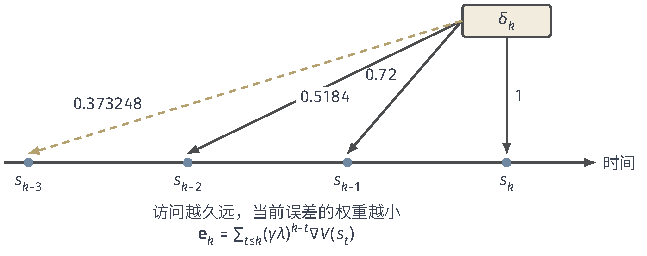
\includegraphics[width=109.583mm]{figures/10-reinforcement-learning/01-problems-and-solving/tikz/rl-learning-traces.pdf}
  \caption{同一个TD误差的后向信用分配。横轴为访问时刻，箭头上的数值来自$\gamma\lambda=0.72$。前向视图把未来误差加给当前状态，后向视图在误差出现时按资格迹更新与过去访问有关的参数。}
  \label{fig:rl-learning-traces}
\end{figure}

\begin{table*}[t]
  \centering
  \small
  \begin{tabularx}{\linewidth}{>{\raggedright\arraybackslash}p{26mm} >{\raggedright\arraybackslash}X >{\raggedright\arraybackslash}X}
    \toprule
    方法 & 改变什么 & 需要保留的边界 \\
    \midrule
    积累迹 & 每次访问都加上特征，旧迹乘$\gamma\lambda$ & 重复访问会累加；等价定理使用固定参数 \\
    替换迹 & 表格或二值特征中，把本次激活分量置1而非继续累加 & 改变重复访问权重；一般稠密特征不能照搬“置1”语义 \\
    真实在线TD & 使用修正的迹与更新，匹配随时间变化的前向目标 & 经典精确等价针对线性表示的在线前向视图，不是任意网络的代数恒等式 \\
    奖励重分配 & 把延迟奖励分配到预测中关键的过去事件 & 保持目标须保证逐轨迹折扣总和相等，或明确等价条件 \\
    \bottomrule
  \end{tabularx}
  \caption{改变信用传播与改变奖励位置并非同一操作。真实在线TD修正参数变化引起的偏差，RUDDER类方法则学习奖励应归到哪些事件。}
  \label{tab:rl-learning-trace-variants}
\end{table*}

真实在线TD的修正正是为了让在线参数变化也有明确的前向解释\scite{rl3-vanseijen2014true}

\Needspace{14\baselineskip}
RUDDER利用序列回报预测，把预测变化归给较早的关键事件\scite{rl3-arjona2019rudder}
在有限回合、未折扣回报下，重分配若满足$\sum_t\widetilde r_t=\sum_t r_t$，就保留逐轨迹总回报；折扣目标则需要$\sum_t\gamma^t\widetilde r_t=\sum_t\gamma^t r_t$，不能只核对未加权总和。预测不完整时还要有残差补偿或另外分析误差。即使奖励位置改得很合适，从未到达过奖励区域的转移与奖励记录也不能凭空告诉模型那里有什么。

% Outline: 3.2.3
\subsection{离策略回报估计与校正}
\label{sec:rl-learning-off-policy}

策略改进后，回放中的旧轨迹仍可利用，但直接平均其回报会评价采集这些轨迹记录的旧策略，而非当前目标策略。我们将前者称为行为策略$\beta$，后者称为目标策略$\pi$。两者共享环境时，轨迹概率的差别来自动作抽样；重要性校正按这一概率比重新加权，使行为策略采集的轨迹记录可用于目标策略评价。前提是目标可能产生的轨迹在行为分布下也有机会出现，否则任何权重都无法补出缺失经验。

先看只有一个决策的教学例。行为策略以概率$1/2$选右，目标策略以概率$0.8$选右。对于“选右后收到奖励”的记录，权重为$0.8/(1/2)=1.6$；对于选左记录，权重为$0.2/(1/2)=0.4$。于是行为抽样后的平均加权回报为$0.8$倍右动作奖励均值加$0.2$倍左动作奖励均值，正好等于目标策略回报。这就是重要性采样（importance sampling）：样本仍来自原分布，但通过权重计算另一分布的期望。

连续多步时，一条动作前缀在目标策略下的概率是各步目标动作概率的乘积，行为策略下同样如此，所以校正权重也相乘。已经发生的$r_t$只需要截至动作$t$的前缀权重，后来的动作不改变这项奖励。定理将这个直觉写成完整轨迹与逐决策两种公式；其中“目标律绝对连续于行为律”正是前述要求，即行为分布不能给目标可能出现的事件零概率。

\begin{theorem}[轨迹与逐决策重要性校正]
  \label{thm:rl-learning-importance-sampling}
  设$H\geq1$为整数，$0\leq\gamma\leq1$，状态与合法动作集有限。固定平稳Markov行为策略$\beta$与目标策略$\pi$，二者使用同一初始分布$\mu_0$及同一联合奖励转移核$p(\mathrm dr,s'\mid s,a)$。令$G_0=\sum_{t=0}^{H-1}\gamma^t r_t$。设目标轨迹律$P_{\mathcal E}^{\pi}$绝对连续于行为轨迹律$P_{\mathcal E}^{\beta}$，且对各$t<H$有$\mathbb E_\pi|r_t|<\infty$。在行为实际产生的历史上记
  \[
    \rho_t=\frac{\pi(a_t\mid s_t)}{\beta(a_t\mid s_t)},\qquad
    W_{u:v}=\prod_{k=u}^{v}\rho_k .
  \]
  则
  \begin{equation}
    \mathbb E_\pi G_0
       =\mathbb E_\beta[W_{0:H-1}G_0]
       =\mathbb E_\beta\left[\sum_{t=0}^{H-1}
                           \gamma^t W_{0:t}r_t\right].
    \label{eq:rl-learning-is}
  \end{equation}
\end{theorem}
\begin{proof}
  对轨迹$\tau=(s_0,a_0,r_0,\ldots,s_H)$，共同初始分布和联合奖励转移核给出按发生顺序的测度乘积
  \[
    P_{\mathcal E}^{\pi}(\mathrm d\tau)
      =\mu_0(s_0)\prod_{t=0}^{H-1}
        \pi(a_t\mid s_t)\,p(\mathrm dr_t,s_{t+1}\mid s_t,a_t).
  \]
  Radon--Nikodym导数在行为轨迹律几乎处处意义下为$W_{0:H-1}$。行为概率为0的历史可任意约定权重版本，例如取0；绝对连续性保证不会遗漏目标质量。对可积回报应用换测度，得到第一个等式。

  再把轨迹截到$r_t,s_{t+1}$，记此前缀为$\tau_{0:t+1}$。对剩余轨迹积分后，两条策略的前缀分布仍由相同环境核与各自动作概率相乘得到，故前缀密度比为$W_{0:t}$。完整轨迹的绝对连续性也保证前缀绝对连续。将换测度分别用于非负的$|r_t|$，得到
  \[
    \mathbb E_\beta[W_{0:H-1}|r_t|]
    =\mathbb E_\beta[W_{0:t}|r_t|]
    =\mathbb E_\pi|r_t|<\infty.
  \]
  因而下面各项期望均存在。由于$r_t$仅依赖该前缀，
  \[
    \mathbb E_\beta[W_{0:H-1}r_t]
    =\mathbb E_\pi[r_t]
    =\mathbb E_\beta[W_{0:t}r_t].
  \]
  对有限个奖励项加权求和，得到逐决策形式。这个前缀论证不要求在目标概率为0的行为历史上，未来概率比也具有条件均值1。
\end{proof}

以网格中一段两步动作前缀为例，若行为动作概率分别为$1/2,1/4$，目标概率分别为$0.8,0.6$，则比率为$1.6,2.4$，乘积为$3.84$。对应奖励对逐决策估计的贡献为$1.6r_0+0.9(3.84)r_1$。概率比不含滑移概率，因为两条策略共享同一转移核；若这些轨迹记录由另一种滑移机制生成，这个消去理由便不存在。

方差问题在最简单的教学模型中就会出现：目标策略必选的两步动作，在行为策略下每步概率都是0.1，故该前缀仅以0.01发生，权重为100。设仅成功前缀末端奖励为1，其余为0且暂取$\gamma=1$，无偏估计量以概率0.01取100，否则取0，均值为1而方差为99。图\ref{fig:rl-learning-is-sampling}把低概率和大权重画在同一条路径上。若行为概率改成0，权重技巧就完全失效。

\begin{figure}[htbp]
  \centering
  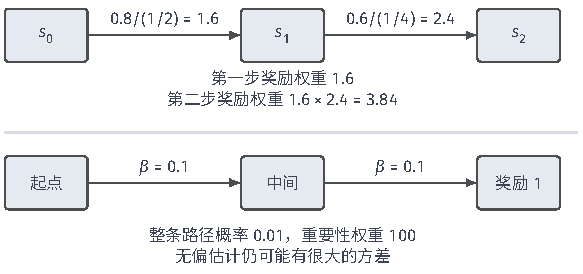
\includegraphics[width=98.651mm]{figures/10-reinforcement-learning/01-problems-and-solving/tikz/rl-learning-is-sampling.pdf}
  \caption{两步重要性权重的乘积。上方为可手算的网格动作前缀，下方为独立的罕见路径教学例；共同环境核不进入比率。宽支持是可校正的前提，大权重则是方差问题。}
  \label{fig:rl-learning-is-sampling}
\end{figure}

直接将过大的总权重截小，会连期望一并改变。在上面的罕见路径例中，若把权重100截为10，平均估计从1降到$0.01\times10=0.1$。要在控制波动时仍评价指定策略，就必须设计不同的误差传播方式或补偿项；下面的多步方法需要分清截断的是当前奖励权重，还是未来误差传回来的系数。

完整概率比积可能随时域增长而剧烈波动。多步自举可以改为传播逐步Bellman误差，并限制较远误差的权重，但是否保留目标策略取决于截断位置。先固定$\pi$，在后继状态对其合法动作按概率求平均，构造
\[
  \delta_t^\pi=r_t+\gamma\sum_a\pi(a\mid s_{t+1})Q(s_{t+1},a)
                       -Q(s_t,a_t).
\]
Retrace使用$c_t=\lambda\min(1,\rho_t)$，从给定$(s_t,a_t)$构造
\begin{equation}
  Q_{\mathrm{ret},t}
   =Q(s_t,a_t)+\sum_{k=t}^{T-1}
        \gamma^{k-t}\left(\prod_{j=t+1}^{k}c_j\right)\delta_k^\pi .
  \label{eq:rl-learning-retrace}
\end{equation}
空积为1。注意第一项误差不乘$\rho_t$，因为这里评价的起始动作已给定；$\pi$期望进入每个Bellman误差，截断系数只控制更远误差的传播。教学例若$\delta_t^\pi=0.4$、$\delta_{t+1}^\pi=-0.2$、$\lambda=0.8$、$\rho_{t+1}=2$，则增量为$0.4+0.9(0.8)(-0.2)=0.256$。以步长$0.5$更新时，起始$Q$增加$0.128$。表\ref{tab:rl-learning-off-policy-targets}比较不同方法的截断位置，尤其要看当前误差与后续迹是否承担不同权重。

\begin{table*}[t]
  \centering
  \small
  \begin{tabularx}{\linewidth}{>{\raggedright\arraybackslash}p{23mm} >{\raggedright\arraybackslash}X >{\raggedright\arraybackslash}X}
    \toprule
    校正方法 & 权重放在哪里 & 目标与不动点 \\
    \midrule
    普通重要性采样 & 完整回报或每步奖励前乘概率比积 & 支持充分时无偏评价$\pi$；方差可能指数增长 \\
    直接截断总权重 & 用$\min(c,W)$替代$W$ & 一般改变期望；没有补偿不能声称仍精确评价$\pi$ \\
    Tree Backup & 多步误差迹用$\lambda\pi(a_t\mid s_t)$ & 以$\pi$期望备份，保留$Q^\pi$不动点；未选分支由估值补足 \\
    Retrace & 迹用$\lambda\min(1,\rho_t)$ & 表格、覆盖等条件下不动点为$Q^\pi$，截断并非直接截回报权重 \\
    V-trace & TD误差前用截断$\rho$，后续迹另截断$c$ & 有限$\bar\rho$一般评价$\pi_{\bar\rho}(a\mid s)\propto\min(\bar\rho\beta(a\mid s),\pi(a\mid s))$；$c$主要改变传播与收敛速度 \\
    \bottomrule
  \end{tabularx}
  \caption{几种离策略多步目标的差别。表格不动点结论不能直接替代有限训练样本和非线性优化分析。}
  \label{tab:rl-learning-off-policy-targets}
\end{table*}

\Needspace{14\baselineskip}
在$Q=Q^\pi$时，给定每个被访问状态动作，$\delta_t^\pi$的条件均值为0；可预测的迹系数不改变这个零点，这是理解Retrace不动点的入口。证明其收缩与控制性质还要利用系数范围和覆盖条件\scite{rl3-munos2016retrace}

\Needspace{18\baselineskip}
V-trace截断当前误差的概率比则会改变条件动作权重，因此具有不同的有效目标策略\scite{rl3-espeholt2018impala}
两者不能统称为“截断只降方差、不改目标”。

% Outline: 3.2.4
\subsection{表格与平均奖励条件下的价值控制}
\label{sec:rl-learning-tabular-control}

固定策略评价给出当前走法的长期回报，控制则用这个评价改变走法。MC控制先用完整回报估计$Q^\pi(s,a)$，再提高当前贪心动作的选择概率；下一批轨迹于是来自改进后的策略。未访问表项仍没有纠错样本。探索起点允许从不同状态动作开始，是额外的交互采样访问机制；软策略在可达状态给各动作保留正概率，却不能让不可达状态自动出现。采用哪种机制都还要检查实际覆盖。

用$V(s)$评价当前策略时，动作已经按该策略平均掉了。要在模型未知时改变动作，保留$Q(s,a)$更直接：每个合法动作各有一项估值，比较这些表项即可选择。一步控制的差异则落在未来如何行动：继续评价包含探索的实际走法、对指定策略平均，或假定下一步选择当前最优动作。这些选择决定下面三个目标，而非只改变算法名称。

一步控制保留统一的更新外形
\begin{equation}
  Q(s_t,a_t)\leftarrow Q(s_t,a_t)
        +\alpha_t[y_t-Q(s_t,a_t)],
  \label{eq:rl-learning-control-update}
\end{equation}
区别在目标$y_t$，具体见表\ref{tab:rl-learning-control-targets}。SARSA把下一次实际选择的动作接上去，因此五元组$(s_t,a_t,r_t,s_{t+1},a_{t+1})$构成更新；Expected SARSA对目标策略的下一动作求期望；Q-learning直接用下一状态的最大估值。

\begin{table*}[t]
  \centering
  \small
  \begin{tabularx}{\linewidth}{>{\raggedright\arraybackslash}p{28mm} >{\raggedright\arraybackslash}X >{\raggedright\arraybackslash}X}
    \toprule
    方法 & 目标$y_t$ & 下一动作由谁决定 \\
    \midrule
    MC控制 & $G_t$ & 整段轨迹中的行为策略，策略改进发生在回报估计之后 \\
    SARSA & $r_t+\gamma Q(s_{t+1},a_{t+1})$ & 当前行为策略实际抽样；同策略版本评价含探索的行为 \\
    Expected SARSA & $r_t+\gamma\sum_a\pi(a\mid s_{t+1})Q(s_{t+1},a)$ & 显式指定目标策略$\pi$；$\pi=\beta$时同策略 \\
    Q-learning & $r_t+\gamma\max_aQ(s_{t+1},a)$ & 目标贪心策略；行为可以继续探索 \\
    \bottomrule
  \end{tabularx}
  \caption{控制更新中的动作来源。终止转移的自举部分均为0；所有最大化都只在合法动作集合中进行。}
  \label{tab:rl-learning-control-targets}
\end{table*}

\begin{example}[一条转移，三个一步目标]
  \label{ex:rl-learning-sarsa-q}
  基准网格中从$(3,1)$向右并到达$(4,1)$，奖励为$-0.04$。教学估值取$Q((4,1),\text{上})=0.8$、$Q((4,1),\text{左})=0.2$，行为概率分别为$0.75,0.25$，下一次恰好选了左。则SARSA目标为$0.14$，Expected SARSA目标为$-0.04+0.9(0.75\times0.8+0.25\times0.2)=0.545$，Q-learning目标为$0.68$。若当前被更新表项为$0.3$、步长为$0.5$，新值分别为$0.22,0.4225,0.49$。这些差异来自目标策略和动作抽样，不是对同一个目标做出了三个互相矛盾的估计。
\end{example}

最大化还会偏爱正的估计噪声。独立教学例中，两个动作的真实值均为0，各估计独立等概率取$-1$或1；最大值以概率$3/4$为1、$1/4$为$-1$，均值为$0.5$。这不是某个动作本来更好，而是“选最大”与“报告它的估值”使用了同一份噪声。

要减少这项选择偏差，可以用一份估计选动作，用另一份估计评价被选动作。Double Q-learning维护两张表$Q^A,Q^B$，随机更新其中一张；更新$A$时先在合法动作中最大化$Q^A$，再把所选动作的$Q^B$值接到奖励后：
\begin{equation}
  a^\star=\argmax_a Q^A(s_{t+1},a),\qquad
  y_t^A=r_t+\gamma Q^B(s_{t+1},a^\star),
  \label{eq:rl-learning-double-q}
\end{equation}
更新$B$时交换两者角色。行为可对两表之和采用$\varepsilon$-贪心。在刚才的理想独立噪声例中，用$A$选择、用独立的$B$评价，被选动作的$B$估值条件均值仍为0。但真实两张表共享环境交互记录，不保证独立，也可能产生低估或其他逼近误差；双估计针对的是选择与评价耦合，而不是通用误差消除器\scite{rl3-hasselt2010double}

表格折扣Q-learning的经典收敛结论要求有限状态动作、有界奖励，每个状态动作被无限访问，并且对每一对$(s,a)$的本地更新步长满足
\[
  \sum_n\alpha_n(s,a)=\infty,\qquad
  \sum_n\alpha_n(s,a)^2<\infty .
\]
条件期望更新是$\mathcal B^*Q-Q$，最优Bellman算子的压缩性控制估值误差，随机逼近处理采样噪声。单条持续轨迹若进了无法返回的区域，即使每一步都探索，也未必满足无限访问条件。SARSA控制还需行为逐渐成为贪心且仍无限探索，通常称为GLIE；持续固定$\varepsilon$的SARSA并非同一个最优性结论\scite{rl1-watkins1992-qlearning,rl3-singh2000convergence}

有些任务关心长期每步产出，而不是折扣总和。例如持续运行的服务系统没有自然终点。此时要显式更换目标。对固定策略$\pi$，若有限链不可约并具有适当回返性质，可定义与起点无关的\term{平均奖励增益}
\[
  g^\pi=\lim_{T\to\infty}\frac1T
      \mathbb E_\pi\sum_{t=0}^{T-1}r_t .
\]
对应的\term{差分价值}衡量相对于长期平均水平的暂时盈亏，满足Poisson方程
\begin{equation}
  g^\pi+h^\pi(s)=R^\pi(s)+\sum_{s'}T^\pi(s'\mid s)h^\pi(s').
  \label{eq:rl-learning-average-poisson}
\end{equation}
对不可约、非周期的有限链，奖励均值有限时，可以先累加有限段奖励，再扣除同样步数的平均收益：
\[
  h_{\mathrm c}^\pi(s)
   =\lim_{H\to\infty}\mathbb E_s^\pi\!\left[
        \sum_{t=0}^{H-1}(r_t-g^\pi)\right].
\]
这里$\mathbb E_s^\pi$表示从$s$启动并执行$\pi$。这个极限比较的是不同起点在进入长期运行状态之前，多得或少得多少期望奖励；它没有把随机级数$\sum_t(r_t-g^\pi)$当作几乎处处收敛的量。上式选定了平稳均值为0的解。因为Poisson方程中$h^\pi+c$仍是解，也可以改取
$h^\pi(s)=h_{\mathrm c}^\pi(s)-h_{\mathrm c}^\pi(s_{\mathrm{ref}})$，令参考状态的值为0。更一般单链任务还要额外处理瞬态状态与极限形式。

\begin{example}[相同长期增益，不同起点差额]
  \label{ex:rl-learning-differential-value}
  固定策略后只有两个状态$x,y$，从任一状态出发，下一步都以各$1/2$的概率到$x$或$y$；在$x$当步得1，在$y$当步得0。这是不可约、非周期的有限链，平稳分布为$(1/2,1/2)$，所以$g^\pi=1/2$。

  从第二步起，两种起点的期望奖励都已为$1/2$。因此对每个$H\geq1$，中心化回报的期望分别为
  \[
    \mathbb E_x^\pi\sum_{t=0}^{H-1}(r_t-\tfrac12)
      =\tfrac12,\qquad
    \mathbb E_y^\pi\sum_{t=0}^{H-1}(r_t-\tfrac12)
      =-\tfrac12.
  \]
  上述极限给出$h_{\mathrm c}^\pi(x)=1/2$、$h_{\mathrm c}^\pi(y)=-1/2$。若改令$h^\pi(y)=0$，则$h^\pi(x)=1$。代回Poisson方程，
  \[
    \tfrac12+1=1+\tfrac12(1+0),\qquad
    \tfrac12+0=0+\tfrac12(1+0).
  \]
  两个状态的长期每步收益相同；差分价值相差1，只表示从$x$起步比从$y$起步多一次奖励1，并非以后每步都多得1。
\end{example}

要将状态差分价值用于动作比较，先固定当前合法动作$a$，此后仍按$\pi$行动。相应的差分动作值为
\[
  \begin{aligned}
    q^\pi(s,a)
      &=R(s,a)-g^\pi
        +\sum_{s'}T(s'\mid s,a)h^\pi(s'),\\
    h^\pi(s)
      &=\sum_{a\in\mathsf A(s)}\pi(a\mid s)q^\pi(s,a).
  \end{aligned}
\]
第一式扣除当前一步的平均增益，再接后继的相对价值；第二式由Poisson方程和按策略平均得到。它不是折扣动作值$Q^\pi$，并与$h^\pi$共享加法常数的约定。令$q$为这项动作值的当前估计、$\widehat g$为长期每步平均奖励的估计。差分SARSA使用下一实际动作的差分值构造一步误差，正步长$\alpha_t$调整动作值，$\alpha_t^g$调整增益：
\[
  \begin{aligned}
    \delta_t&=r_t-\widehat g+q(s_{t+1},a_{t+1})-q(s_t,a_t),\\
    q(s_t,a_t)&\leftarrow q(s_t,a_t)+\alpha_t\delta_t,\qquad
    \widehat g\leftarrow\widehat g+\alpha_t^g\delta_t .
  \end{aligned}
\]
\Needspace{14\baselineskip}
差分Q-learning以$\max_a q(s_{t+1},a)$替代下一实际动作值，并配合增益更新及归一化。R-learning的经典形式也维护差分动作值和平均奖励，但增益只在规定的贪心更新条件下调整\scite{rl3-schwartz1993rlearning}
典型增益误差是$r_t+\max_aq(s_{t+1},a)-\max_aq(s_t,a)-\widehat g$。名称相近不表示更新条件完全相同。

\Needspace{14\baselineskip}
可证明的平均奖励算法还要列明弱连通或单链条件、参考函数、步长及访问要求\scite{rl3-wan2021average}
式\eqref{eq:rl-learning-average-poisson}没有折扣压缩因子，不能照搬Q-learning的折扣证明。

% Outline: 3.2.5
\subsection{函数逼近下的价值学习与稳定性}
\label{sec:rl-learning-approximation}

网格中的状态可以逐个存表，图像或连续状态则难以枚举。函数逼近（function approximation）改用同一组参数表示许多状态的价值：在线性表示$V_{\bm{\theta}}(s)=\bm{\phi}(s)^\top\bm{\theta}$中，已知特征$\bm\phi(s)$决定各参数怎样影响该状态。共享参数使一条经验也能改变未访问状态的预测，同时让不同状态的更新相互牵连。换成网络进一步扩大函数类，却不会自动保留表格更新的压缩结构。

共享参数的效果可以用一个独立线性例子看清。取$\bm\phi(s_1)=(1,0)^\top$、$\bm\phi(s_2)=(1,1)^\top$，参数$\bm\theta=(0.2,0.3)^\top$，两个预测分别为$0.2,0.5$。在$s_1$收到目标$0.4$，用步长$0.5$做半平方误差下降，得到$\bm\theta'=(0.3,0.3)^\top$；没有访问$s_2$，其预测也从$0.5$变成$0.6$。这使样本能够泛化，也意味着一次局部更新可能改变其他地方正确的预测。后面要检查的稳定性，正来自这种联动与自举目标的配合。

三种误差分别回答不同的问题。真实价值误差问预测离$V^\pi$有多远，但通常拿不到这个答案作标签；Bellman误差问当前预测是否与自身的一步备份一致。共享特征还带来第三个问题：备份后的整组状态值未必能由当前特征表示，例如只允许常数函数时，不可能同时表示两个不同目标值。把备份替换成函数类内加权平方距离最近的可表示函数，就是这里的投影；投影Bellman误差只比较这份可表示目标与当前预测。接下来用$d$指定各状态的权重，决定哪些状态的拟合偏离占更大比重，不能将三种误差都叫作同一个训练损失。

先固定策略$\pi$和采样分布$d$，暂设所讨论的有限状态上$d(s)>0$，令$\bm D$为以$d(s)$作对角元的矩阵。这里的$d$是指定的误差权重，不一定等于策略的折扣占用$d^\pi$。表\ref{tab:rl-learning-value-objectives}中的$\mathcal B^\pi$含真正的环境条件期望；$\Pi_d$把目标投影到线性特征能表示的空间，最近程度按$\|u\|_d^2=\sum_s d(s)u(s)^2$计量。

有限状态下，整组价值是一份实向量，线性特征能表示的向量构成线性子空间。正权重$d$使加权平方距离对应一个内积，最近点唯一，剩余误差与该子空间正交。这就是这里采用的正交投影条件；更一般的实Hilbert空间中，需要子空间非空且闭。非凸网络类可能有多个同样近的函数，不能直接继承唯一性或后面的线性矩阵式。投影与函数空间条件可参考\BookChapterRef{chap:functional-analysis-and-approximation}{卷1《数学准备：计算、分析与几何》中讨论函数空间的章节}。

\begin{table*}[t]
  \centering
  \small
  \begin{tabularx}{\linewidth}{>{\raggedright\arraybackslash}p{30mm} >{\raggedright\arraybackslash}X >{\raggedright\arraybackslash}X}
    \toprule
    误差目标 & 公式 & 需要知道或估计什么 \\
    \midrule
    均方价值误差 & $\lVert V_{\bm{\theta}}-V^\pi\rVert_d^2$ & 真实价值$V^\pi$，通常不能直接监督 \\
    均方Bellman误差（MSBE） & $\lVert \mathcal B^\pi V_{\bm{\theta}}-V_{\bm{\theta}}\rVert_d^2$ & 先对奖励和后继求条件期望，再平方 \\
    均方投影Bellman误差（MSPBE） & $\lVert\Pi_d\mathcal B^\pi V_{\bm{\theta}}-V_{\bm{\theta}}\rVert_d^2$ & 投影后的备份；依赖特征空间和采样权重 \\
    \bottomrule
  \end{tabularx}
  \caption{固定策略下的三种误差。把样本TD误差平方，并不会自动得到其中的MSBE。}
  \label{tab:rl-learning-value-objectives}
\end{table*}

同一个状态可能出现多个随机后继。将每次样本误差平方后平均，与先平均误差再平方，是两个不同的计算；前者还惩罚后继随机性造成的波动。下面的条件方差分解说明为什么这种差异甚至会改变最优参数。

\Needspace{10\baselineskip}
固定本次更新的参数$\bm\theta$。令$x$表示Bellman条件：评价状态价值时为$s$，评价动作价值时为$(s,a)$。若样本TD误差$\delta_{\bm\theta}$二阶可积，条件均值与条件方差满足
\begin{equation}
 \mathbb E[\delta_{\bm\theta}^2\mid x]
  =\bigl(\mathbb E[\delta_{\bm\theta}\mid x]\bigr)^2
     +\operatorname{Var}(\delta_{\bm\theta}\mid x).
 \label{eq:rl-learning-td-variance}
\end{equation}
条件中心化误差的均值为0，展开平方的交叉项因而消失。应用到TD时，最后一项还可能随参数变化，所以最小化样本平方损失一般不等于最小化Bellman均值残差。二阶可积保证这几项均有定义；它不要求相邻转移独立。

\begin{example}[两个后继使最优参数改变]
  \label{ex:rl-learning-double-sampling}
  这是独立于基准网格的单参数教学例：在固定状态$s$，奖励为1、$\gamma=1/2$，下一状态等概率为$u,v$；令$V_\theta(s)=\theta$、$V_\theta(u)=0$、$V_\theta(v)=2\theta$，只在$s$处度量Bellman残差。两种样本TD误差为$1-\theta$和1。因此
  \[
    \bigl(\mathbb E\delta_\theta\bigr)^2=(1-\theta/2)^2,\qquad
    \mathbb E\delta_\theta^2=\tfrac12(1-\theta)^2+\tfrac12.
  \]
  前者在$\theta=2$最小，后者在$\theta=1$最小；差值为$\theta^2/4$，正是依赖参数的条件方差。在$\theta=2$处Bellman平均残差已经为0，样本平方损失却仍会把参数往回推。这比仅展示一项常数噪声更直接地说明了目标不等价。
\end{example}

若目标确实是减少Bellman条件均值残差，就需要对MSBE本身求导，而不能直接把样本平方损失的梯度当作它。将MSBE乘$1/2$只消去平方求导中的系数2，不改变最小化方向。沿用$m_{\bm\theta}(x)=\mathbb E[\delta_{\bm\theta}\mid x]$，若可交换求导与条件期望，则
\begin{equation}
  \nabla_{\bm{\theta}}\frac12\mathbb E_x[m_{\bm{\theta}}(x)^2]
    =\mathbb E_x\!\left[
        \mathbb E(\delta_{\bm{\theta}}\mid x)\,
        \mathbb E(\nabla_{\bm{\theta}}\delta_{\bm{\theta}}\mid x)
      \right].
  \label{eq:rl-learning-msbe-gradient}
\end{equation}
关键是两个条件均值的乘积。用同一后继样本估计两因子，会得到$\mathbb E[\delta_{\bm{\theta}}\nabla\delta_{\bm{\theta}}\mid x]$，多出两因子的条件协方差；在可微条件下也可看成条件方差梯度的一半。

\term{双重采样}要求给定同一个$x$后，独立抽两份后果$\xi,\widetilde\xi$，用$\delta_{\bm{\theta}}(x,\xi)\nabla\delta_{\bm{\theta}}(x,\widetilde\xi)$估计该乘积。图\ref{fig:rl-learning-double-sampling}强调两条支路必须条件独立，而不是从回放中随意取两个不同状态。对状态价值，固定$s$后还要独立按$\pi$抽动作和后果；对动作价值，固定$(s,a)$后独立抽奖励、后继及目标所需随机量。普通在线轨迹通常不能要求环境从原状态再独立执行一次；确定性后继、可查询生成模型或某些特殊结构须单独判断\scite{rl3-zhu2020borrowing}

\begin{figure*}[t]
  \centering
  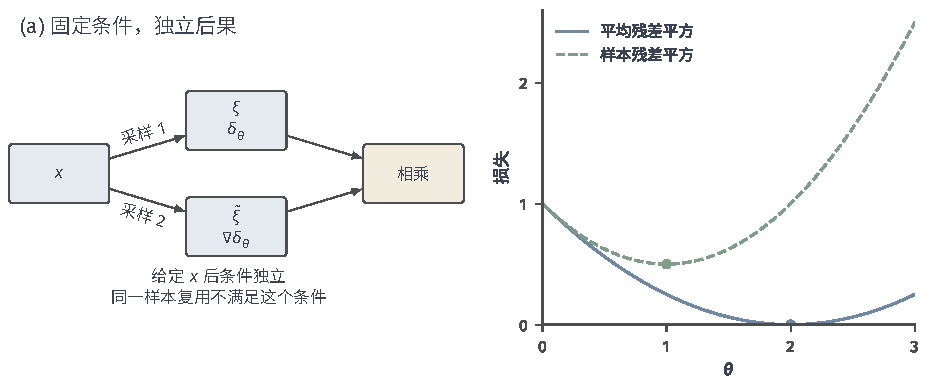
\includegraphics[width=157.406mm]{figures/10-reinforcement-learning/01-problems-and-solving/tikz/rl-learning-double-sampling.pdf}
  \caption{双重采样针对条件均值乘积。左侧两条独立支路保持同一个条件变量$x$；右侧曲线按示例\ref{ex:rl-learning-double-sampling}的解析公式绘制，展示两个损失的最小值不在同一参数处。}
  \label{fig:rl-learning-double-sampling}
\end{figure*}

常见的半梯度TD采取另一条路线：对自举目标停止求导，只执行
\[
  \bm{\theta}\leftarrow\bm{\theta}
       +\alpha\delta_{\bm{\theta}}
                    \nabla_{\bm{\theta}}V_{\bm{\theta}}(s).
\]
“半”表示没有求目标中下一价值对参数的导数。它不是式\eqref{eq:rl-learning-msbe-gradient}的随机梯度，因而不能借用该损失下降作为稳定性证明。在线性、同策略且采样权重与策略平稳分布匹配时，可用投影Bellman方程分析；离策略权重会破坏这条论证。表\ref{tab:rl-learning-fitted-methods}把这种逐步递推与批量方程、重复回归放在同一个评价或控制接口下比较。

在线性TD中，记$\bm\phi=\bm\phi(s)$、$\bm\phi'=\bm\phi(s')$，分别为当前和后继特征，撇号不是导数。平均更新为0要求$\mathbb E[\bm\phi\delta]=\bm0$；把$\delta=r+\gamma\bm\phi'^{\top}\bm\theta-\bm\phi^{\top}\bm\theta$代入并整理，就得到$\bm A\bm\theta=\bm b$。这里的期望按$s\sim d$、$a\sim\pi(\cdot\mid s)$、$(r,s')\sim p(\cdot,\cdot\mid s,a)$的固定策略样本计算；使用行为策略记录时需另作离策略校正。

这为批量求解提供了入口：最小二乘时序差分（least-squares temporal difference, LSTD）用许多记录估计$\bm A,\bm b$，再解方程；最小二乘策略迭代（least-squares policy iteration, LSPI）把这种动作值评价与贪心改进交替执行。拟合Q迭代（fitted Q-iteration, FQI）则不要求线性方程，而是每轮冻结旧$Q$，为记录构造新标签，再让回归器拟合。下面的表按这些不同求解任务汇总。

\begin{table*}[t]
  \centering
  \small
  \begin{tabularx}{\linewidth}{>{\raggedright\arraybackslash}p{23mm} >{\raggedright\arraybackslash}X >{\raggedright\arraybackslash}X}
    \toprule
    方法 & 解什么问题 & 表示、转移记录与适用边界 \\
    \midrule
    半梯度TD & 用样本逼近Bellman不动点，不对目标求全导数 & 线性同策略有专门保证；一般网络不是某个MSBE的下降法 \\
    LSTD & 解$\bm{A}\bm{\theta}=\bm{b}$，其中$\bm{A}=\mathbb E[\bm{\phi}(\bm{\phi}-\gamma\bm{\phi}')^\top]$、$\bm{b}=\mathbb E[r\bm{\phi}]$ & 固定策略线性评价；离策略版本需概率比等校正与矩阵可解条件 \\
    LSPI & 交替做动作值的LSTD评价与贪心改进 & 线性动作特征、同一批固定转移记录反复用于不同目标策略；需要相关状态动作覆盖 \\
    拟合Q迭代（FQI） & 冻结旧$Q$，回归$r+\gamma\max_aQ_{\mathrm{old}}(s',a)$ & 可用非线性回归器；控制误差包含回归误差、函数类封闭性与分布迁移 \\
    \bottomrule
  \end{tabularx}
  \caption{评价、控制与求解方式的差别。批量最小二乘减少逐步更新噪声，不会消除状态动作记录缺失或错误目标。}
  \label{tab:rl-learning-fitted-methods}
\end{table*}

\Needspace{20\baselineskip}
LSTD直接估计线性不动点方程的矩阵与向量，再求解参数\scite{rl3-bradtke1996lstd}
它省去逐步梯度迭代，但样本矩阵病态时仍需正则化和数值诊断，不能把可写成线性方程理解为总能稳定求逆。

LSPI把这种评价接口接到策略迭代：评价当前策略，按动作值改进，再重新构造与新策略相应的评价方程。固定转移样本的复用依赖行为策略记录对所需状态动作的覆盖，不是一次解线性方程便得到全局最优策略\scite{rl3-lagoudakis2003lspi}

FQI则冻结上一轮动作值，将新的Bellman目标交给监督回归器。它允许树模型等非梯度回归工具；每轮拟合误差以及从训练转移记录的状态动作抽样分布到部署策略访问分布的变化，仍会影响最终控制质量。三者提供了不同计算接口，不能只按是否使用梯度分类\scite{rl3-ernst2005tree}

一个完全线性的反例足以说明离策略、自举与共享参数同时出现的风险。Baird反例有7个状态、8个参数，奖励全为0，$\gamma=0.99$\scite{rl3-baird1995residual}
目标策略总选实线动作，转到状态7；行为策略以$1/7$选实线动作，以$6/7$选虚线动作，后者均匀转到上方6个状态。行为链的平稳分布为均匀分布。特征取
\[
  \bm{\phi}(i)=\frac{2\bm{e}_i+\bm{e}_8}{\sqrt5}\quad(1\leq i\leq6),
  \qquad
  \bm{\phi}(7)=\frac{\bm{e}_7+2\bm{e}_8}{\sqrt5}.
\]
令$\bm{\Phi}$的第$i$行为$\bm{\phi}(i)^\top$，$\bm{D}=\bm{I}/7$，$\bm{T}^\pi=\bm{1}\bm{e}_7^\top$。对带一步重要性比的半梯度TD，固定当前参数、按行为平稳样本取期望，漂移为
\begin{equation}
  \mathbb E[\Delta\bm{\theta}\mid\bm{\theta}]
     =\alpha\bm{M}\bm{\theta},\qquad
  \bm{M}=\bm{\Phi}^\top\bm{D}
                   (\gamma\bm{T}^\pi-\bm{I})\bm{\Phi}.
  \label{eq:rl-learning-baird-matrix}
\end{equation}
重要性比修正了给定状态的动作分布，却没有把行为状态权重$\bm{D}$换成目标状态权重。

在不变的对称子空间$\theta_1=\cdots=\theta_6=a$、$\theta_7=b$、$\theta_8=c$中，该漂移作用为
\begin{equation}
  \begin{pmatrix}\dot a\\\dot b\\\dot c\end{pmatrix}
  =
  \frac1{35}
  \begin{pmatrix}
    -4 & 1.98 & 1.96\\
     0 & -0.01 & -0.02\\
    -12 & 5.92 & 5.84
  \end{pmatrix}
  \begin{pmatrix}a\\b\\c\end{pmatrix}.
  \label{eq:rl-learning-baird-reduced}
\end{equation}
未除35的矩阵具有特征多项式$z(z^2-1.83z+0.26)$，因此漂移特征值为$0$、约$0.04785009$和$0.00443562$。例如较大的正特征值对应$(a,b,c)\approx(0.34124745,-0.01187117,1)$。若用期望更新作确定性迭代，沿这个方向每步乘$1+\alpha(0.04785009)>1$；在对应平均常微分方程中则指数增长。即使采用趋零且和发散的正步长，该方向的乘积仍不衰减。由此看到的是平均动力学的不稳定方向，而不只是某次随机运行的波动；随机更新还需相应随机逼近分析，不能把独立平稳样本的期望等式不加说明地当成任意相关轨迹下的参数均值递推。真实价值是0，函数类完全能表示它，问题出在更新动力学。

上述反例中，真实零价值在函数类内，平均更新仍有发散方向；单靠表示能力无法修复它。梯度TD方法为固定策略的线性评价改造目标和递推。对行为策略$\beta$的平稳经验，记$\bm\phi_t=\bm\phi(s_t)$、$\bm\phi_{t+1}=\bm\phi(s_{t+1})$，并用$\rho_t=\pi(a_t\mid s_t)/\beta(a_t\mid s_t)$校正动作分布；目标动作仍须由行为策略支持。由这些当前和后继特征定义不动点矩阵$\bm A$、奖励向量$\bm b$及特征二阶矩$\bm C$：
\[
  \bm{A}=\mathbb E_\beta[\rho_t\bm{\phi}_t
          (\bm{\phi}_t-\gamma\bm{\phi}_{t+1})^\top],\quad
  \bm{b}=\mathbb E_\beta[\rho_t r_t\bm{\phi}_t],\quad
  \bm{C}=\mathbb E_\beta[\bm{\phi}_t\bm{\phi}_t^\top].
\]
若$\bm C$正定，则MSPBE为
$(\bm b-\bm A\bm\theta)^\top\bm C^{-1}
 (\bm b-\bm A\bm\theta)$。

辅助向量的作用是把一个难直接估计的乘积拆开。令残差向量$\bm b-\bm A\bm\theta$固定，所需$\bm w$应满足$\bm C\bm w=\bm b-\bm A\bm\theta$；第一条递推用样本逐渐追踪这个解，第二条再用它调整价值参数。GTD2属于梯度时序差分（gradient temporal difference, GTD）方法，其2标识针对投影Bellman误差的版本。这里称双时间尺度，是要求$\bm w$的追踪比$\bm\theta$的变化快，近似形成“先估计当前需要的均值，再据它改变参数”的关系，而非必须开两种物理时钟。

GTD2用辅助向量$\bm w$跟踪$\bm C^{-1}(\bm b-\bm A\bm\theta)$，例如双时间尺度更新
\begin{align}
  \bm w&\leftarrow\bm w+\alpha_t^w
     [\rho_t\delta_t-\bm\phi_t^\top\bm w]\bm\phi_t,
     \nonumber\\
  \bm\theta&\leftarrow\bm\theta+\alpha_t\rho_t
     (\bm\phi_t-\gamma\bm\phi_{t+1})(\bm\phi_t^\top\bm w).
  \label{eq:rl-learning-gtd2}
\end{align}
辅助变量把难以直接估计的期望乘积拆成两个受控的递推，快变量在慢变量变化之前近似跟踪所需均值。

\Needspace{24\baselineskip}
GTD早期版本以期望TD更新的平方范数为目标；GTD2针对MSPBE；TDC采用TD加校正的形式，在同一线性目标下组织更新；emphatic TD则通过跟随迹重设状态权重，例如$F_t=i_t+\gamma\rho_{t-1}F_{t-1}$中$i_t$指定关注程度，以改变离策略投影的稳定性条件。它们并非都在优化同一个无权Bellman残差。收敛定理还需固定策略、特征与重要性比的矩条件、行为链覆盖、矩阵条件以及合适步长；双时间尺度分析常要求$\alpha_t/\alpha_t^w\to0$。这些评价结论没有直接证明深度控制稳定\scite{rl3-sutton2009fast,rl3-sutton2016emphatic}

% Outline: 3.2.6
\subsection{深度价值控制的训练机制}
\label{sec:rl-learning-dqn}

表格中更新一个状态动作，只修改一项数值。深度Q网络（deep Q-network, DQN）用神经网络一次输出或计算动作价值，同一参数会影响许多表项，还会进入后继目标。若每改一次预测，目标也立刻跟着改，训练就不断追逐正在移动的数值。先暂时固定一份旧参数来算标签，再让当前网络拟合它，承接了FQI的短期固定目标思路。

目标移动之外，连续采样还使相邻经验高度相关，少数极端TD误差也可能主导一次梯度。DQN用延迟参数生成目标，减缓自举目标随在线参数移动；把真实经验存入回放再抽样，减少相邻样本在训练批中的相关性；限制大误差的梯度幅度，避免极端残差主导更新。它们改变的是样本组织和短期回归过程，不是任意网络的收敛证明。

记有限回放记录组为$D$，按指定回放权重抽取记录的经验抽样律为$\widehat P_D$。其状态边缘记为$\widehat P_D^S$。每次训练按$\widehat P_D$取记录$(s,a,r,s',z)$，其中$z=1$仅表示环境真正终止。我们要减小在线网络对记录动作的预测与停止求导目标的差；目标先在$s'$的合法动作中找最高延迟估值，再加已观察奖励。记在线参数$\bm\theta$、延迟参数$\bar{\bm\theta}$，得到
\begin{equation}
  y=r+\gamma(1-z)\max_{a'\in\mathsf A(s')}Q_{\bar{\bm\theta}}(s',a'),
  \qquad
  L(\bm\theta)=\mathbb E_{\widehat P_D}
       \ell_\kappa\bigl(y-Q_{\bm\theta}(s,a)\bigr),
  \label{eq:rl-learning-dqn-loss}
\end{equation}
其中$\ell_\kappa(u)=u^2/2$当$|u|\leq\kappa$，否则为$\kappa(|u|-\kappa/2)$。这个Huber形式使大误差的导数限幅。$y$在该次更新中停止求导，目标网络不从这条损失直接反向传播。图\ref{fig:rl-learning-dqn}把两条参数路径分开。

\begin{figure*}[t]
  \centering
  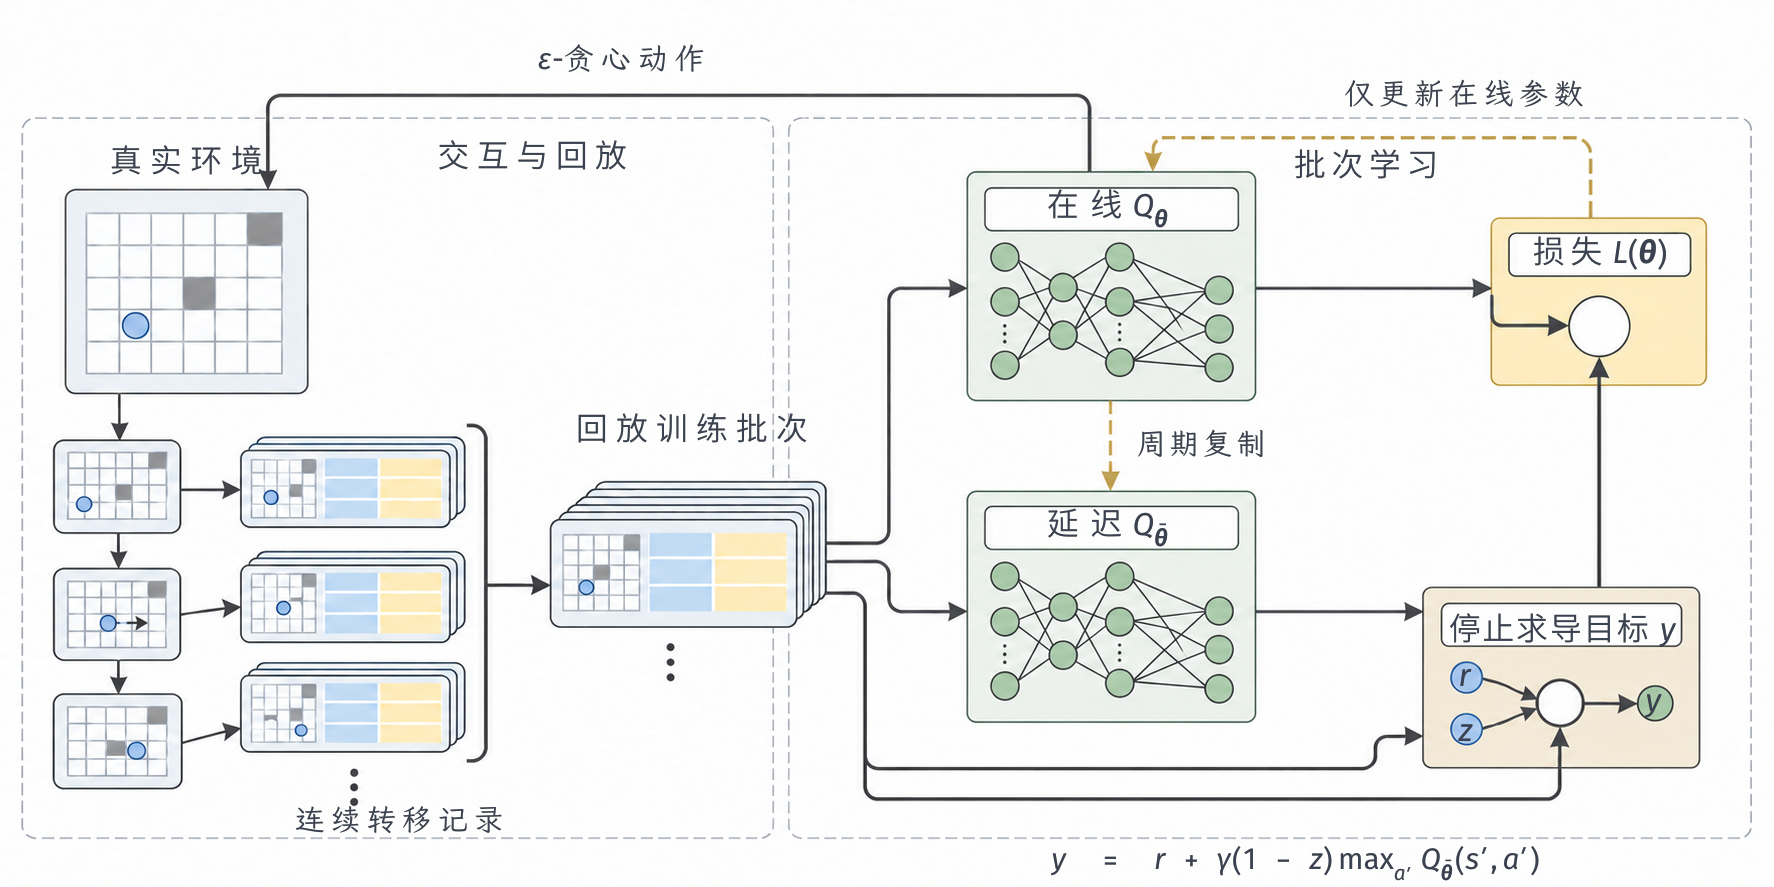
\includegraphics[width=157.400mm]{figures/10-reinforcement-learning/01-problems-and-solving/generated/rl-learning-dqn/figure.png}
  \caption{DQN的交互回放与批次学习。真实转移写入回放，在线网络给出被选动作的估值，延迟网络构造后继目标。在线与延迟网络之间的纵向虚线表示周期复制，外侧虚线表示只更新在线参数的损失梯度；目标分支停止求导。网格、记录卡片和神经节点仅示意部件职责，不规定基准网格布局、批量大小或网络结构。}
  \label{fig:rl-learning-dqn}
\end{figure*}

\begin{algorithm}[包含交互记录采集的DQN循环]
  \label{alg:rl-learning-dqn}
  \begin{algorithmic}[1]
    \Require 网络$\bm\theta$、空回放$D$、批量大小$B$、目标同步间隔$C$、更新频率、合法动作接口
    \State 置$\bar{\bm\theta}\gets\bm\theta$，从环境获得起始状态$s$
    \For{每个真实环境步$t$}
      \State 用当前$Q_{\bm\theta}$的$\varepsilon_t$-贪心策略在$\mathsf A(s)$中选择$a$
      \State 执行$a$，观察$r,s'$及真正终止标记$z$，将$(s,a,r,s',z)$写入$D$
      \If{已满足回放预热数量且到达更新时刻}
        \State 均匀抽取$B$条记录，按式\eqref{eq:rl-learning-dqn-loss}计算停止求导的目标$y_i$
        \State 对$B^{-1}\sum_i\ell_\kappa(y_i-Q_{\bm\theta}(s_i,a_i))$做规定次数梯度更新
      \EndIf
      \If{目标网络更新计数达到$C$}
        \State $\bar{\bm\theta}\gets\bm\theta$，重置同步计数
      \EndIf
      \State 若真正终止或环境因时间上限要求重置，则重置并取得新起点；否则令$s\gets s'$
      \State 仅时间截断的记录仍令$z=0$，并保留重置前的$s'$用于自举
    \EndFor
    \Ensure 在线网络及与训练探索策略区分的评估策略
  \end{algorithmic}
\end{algorithm}

算法\ref{alg:rl-learning-dqn}中的$C$按环境步还是梯度步计数必须在实现中固定。取示例\ref{ex:rl-learning-sarsa-q}的一条记录，若延迟网络最大值为$0.8$、在线被选动作值为$0.3$，则$y=0.68$、残差为$0.38$。当$\kappa=1$，对该输出的梯度为$-0.38$；在仅这一标量可训练、学习率$0.1$的教学网络中，新输出为$0.338$。真实共享网络还会改变其他状态动作，不能把这个标量更新当作一般网络输出的精确变化。

原始DQN在Atari像素输入、固定动作重复与预处理协议下检验了上述机制\scite{mnih2015}
回放减少相邻样本在同一批中的相关性，也允许同一真实经验参与多次更新；这不等于新增了独立采集的环境转移样本。目标网络固定一个短期回归目标，但同步时目标仍会改变。奖励裁剪也改变了训练目标，不能把所有具体设计视为任何任务都适用的定理。

后续部件针对不同的误差来源。表\ref{tab:rl-learning-dqn-components}保留每项实际改变的公式，便于区分表示改造、抽样改变与目标改变。优先回放中，$N$是当前缓冲区的记录数，$i$编号其中一条记录，$P(i)$是归一化抽样概率。指数$p\geq0$控制优先程度，$p=0$恢复均匀抽样；$\epsilon>0$使零残差记录仍有机会被抽到。校正指数$\eta_{\mathrm{IS}}\in[0,1]$控制向均匀缓冲目标补偿的程度，不是抽样概率本身。

有些状态中各动作的回报都差不多，逐动作独立表示会重复学习共同部分。Dueling结构把预测拆成状态共有的$V(s)$与动作差异$A(s,a)$，再对动作差异中心化；这里的$A$先表示网络输出之间的相对量。优先回放解决另一问题：同样抽一次记录，不同记录对当前误差的纠正作用可能不同，因而提高大残差记录的抽样概率，但这会改变经验损失的权重，需要相应校正。参数噪声则在一次扰动下共同改变许多动作评分，使探索发生在整份价值函数的参数上。这三个动机与Double DQN的选择偏差不同，下面分别列出机制。

NoisyNet式中的$\bm W,\bm M,\bm\Sigma,\bm E$形状相同；$\bm M$是可学习的均值权重，$\bm\Sigma$是可学习的噪声尺度系数，$\bm E$是每次扰动时抽取的零均值随机噪声，$\odot$表示逐元素乘法。训练调整前两者，噪声本身按所选分布重采样；这区分了学到的扰动强度和一次抽样结果。

\begin{table*}[t]
  \centering
  \small
  \begin{tabularx}{\linewidth}{>{\raggedright\arraybackslash}p{26mm} >{\raggedright\arraybackslash}X >{\raggedright\arraybackslash}X}
    \toprule
    部件 & 机制或公式 & 不能由它推出什么 \\
    \midrule
    Double DQN & 在线网络选$a^\star=\argmax_aQ_{\bm\theta}(s',a)$，延迟网络评价$Q_{\bar{\bm\theta}}(s',a^\star)$ & 两个网络仍相关，不能保证完全无偏 \\
    Dueling结构 & $Q(s,a)=V(s)+A(s,a)-|\mathsf A(s)|^{-1}\sum_bA(s,b)$ & 分解改善共享表示，不代表学到了独立可识别的真实优势 \\
    优先回放 & $P(i)\propto(|\delta_i|+\epsilon)^p$，权重$w_i\propto(NP(i))^{-\eta_{\mathrm{IS}}}$ & 非均匀抽样改变损失权重；$\eta_{\mathrm{IS}}<1$通常只作部分校正 \\
    NoisyNet & 权重写成$\bm W=\bm M+\bm\Sigma\odot\bm E$，学习噪声尺度 & 参数噪声与逐步随机动作不同，不自动保证长程覆盖 \\
    \bottomrule
  \end{tabularx}
  \caption{深度价值学习中的四种机制。它们分别改变目标、表示、回放记录抽样和探索参数，不能只用“更稳定”概括。}
  \label{tab:rl-learning-dqn-components}
\end{table*}

Double DQN在目标中分开动作选择与评价，避免同一次最大化总是同时选中偏高噪声。在线网络与目标网络仍共享训练历史，因此这不是两个独立无偏估计器，改动也不自动消除所有过估计\scite{rl3-hasselt2016deep}

Dueling用均值中心化消除$V$与$A$任意加减常数的代数歧义，使不同动作能够共享状态评价。但中心化后的$A$不必等于某个给定策略的真实优势；它首先是网络分解中的一个参数化量\scite{rl3-wang2016dueling}

优先回放若以固定缓冲区的均匀经验损失为目标，取$\eta_{\mathrm{IS}}=1$并保留正确的$1/(NP(i))$因子，可以对当前抽样分布校正；常见的批内最大值归一化、过期优先级和逐渐增加$\eta_{\mathrm{IS}}$都需要单独说明\scite{rl3-schaul2016prioritized}

\Needspace{28\baselineskip}
NoisyNet把可学习噪声加入网络参数，一次参数扰动会同时影响多个动作评分，其作用范围不同于逐步$\varepsilon$随机动作\scite{rl3-fortunato2018noisy}
噪声采样频率和尺度学习规则决定探索的时间相关性，但参数随机并不自动保证访问到远处关键状态。

组合系统必须用受控消融解释。Rainbow在57个ALE游戏、2亿帧训练的具体配置中，逐一去掉Double、优先回放、dueling、多步、分布式目标和参数噪声等组件；论文中的优先回放与多步移除影响较大，Double与dueling对中位汇总的影响较小且依游戏而异。这是已组合系统内的条件贡献，不是组件在所有任务上的独立效应。其评估每隔一百万环境步进行一次，并使用最好快照，还涉及no-op和human-starts协议；因此不能把报告值当作预先约定最终检查点的无选择偏差估计\scite{rl3-hessel2018rainbow}

Agent57进一步结合内外在价值、跨时间尺度策略族、回合级元控制器及更长的序列训练。它回答的是更强探索与记忆如何组成系统，不是与Rainbow使用相同总预算的一次单因素试验。把论文中的表现差异归因于某一个部件，必须先统一交互、网络、回放与评估口径；无法统一时，只陈述各自协议下的证据。需要过去观测与动作记录的DRQN与R2D2将在第\ref{chap:rl-information}章讨论，不能把缺少过去观测与动作记录简单归为网络太小\scite{rl3-badia2020agent57}

% Outline: 3.2.7
\subsection{回报分布与控制充分表示}
\label{sec:rl-learning-distributional}

两个动作的期望回报相同，实际后果仍可能很不同。在独立教学例中，路径A总回报恒为$0.5$，路径B等概率得到$-0.5$或$1.5$；均值均为$0.5$，但只有B会出现较低和较高的结果。只存一个均值无法保留这项区别。这里另设了奖励分布，并不声称基准网格存在这两条精确路径；图\ref{fig:rl-learning-return-distributions}展示的就是这两个指定分布。

令$Z^\pi(s,a)$为给定状态动作之后的随机折扣回报。\term{分布式价值学习}（distributional value learning）学习的是整个回报分布，而非仅其均值。分布Bellman关系为
\begin{equation}
  Z^\pi(s,a)\ \overset{D}{=}\ %
    r+\gamma Z^\pi(s',a'),\qquad
  (s',r)\sim p(\cdot,\cdot\mid s,a),\quad a'\sim\pi(\cdot\mid s').
  \label{eq:rl-learning-distributional-bellman}
\end{equation}
右侧的未来随机回报按给定$s',a'$的条件分布抽取，不能误把它理解成一条确定性递推。

\begin{figure}[htbp]
  \centering
  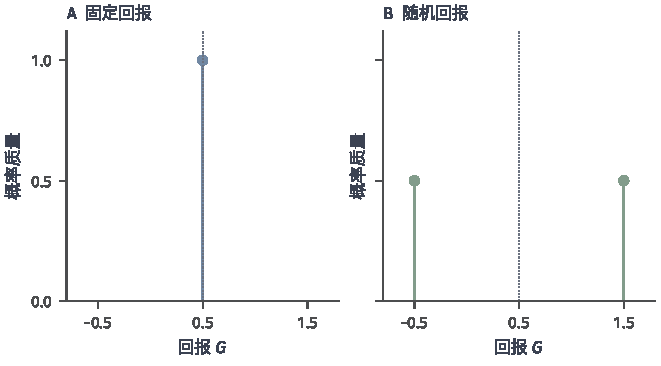
\includegraphics[width=112.000mm]{figures/10-reinforcement-learning/01-problems-and-solving/matplotlib/rl-learning-return-distributions.pdf}
  \caption{相同期望不意味着相同回报分布。两图为人工指定的离散分布，虚线均位于期望$0.5$；这里的不确定性是回报本身的随机性，不是估计参数的置信区间。}
  \label{fig:rl-learning-return-distributions}
\end{figure}

表示一个分布，需要决定保存哪些回报值和多少概率。可以预先固定回报刻度，让模型学习每一刻度附近有多少质量；也可以固定概率刻度，让模型学习对应的回报位置。后一种位置是分位数：$\tau$分位把回报划分到至少$\tau$的概率不超过该值、至少$1-\tau$的概率不低于该值。离散分布可能没有唯一分位位置，后文会给出精确的不等式条件。分位输出与均值输出回答不同问题，不能用普通对称平方误差训练后就称其为分位数。

C51把质量放在固定支撑点$z_1,\ldots,z_N$上，学习各点概率；Bellman变换后的原子$r+\gamma z_j$要按距离插值投影回固定支撑，支撑范围之外的质量会被截到端点。QR-DQN反过来固定每个原子的概率$1/N$，学习分位位置$\theta_i(s,a)$；IQN以随机分位水平$\tau$作为网络输入，表示一个条件分位函数。这三个表示对支撑范围、分辨率和采样方式的限制不同。

要学习分位位置，需要让高分位输出对正残差比负残差更敏感，而不是像平方回归那样都追向均值。以分位回归为例，令$\tau_i=(i-\tfrac12)/N$，$a^\star$是在后继合法动作中按估计均值选出的贪心动作，目标样本为$z'_j=r+\gamma\theta_j(s',a^\star)$。对$u=z'_j-\theta_i(s,a)$，将Huber误差按分位水平非对称加权，再对全部$N^2$对输出和目标平均：
\[
  \rho_{\tau_i}^{\kappa}(u)
      =|\tau_i-\mathbf1\{u<0\}|\frac{\ell_\kappa(u)}{\kappa},
  \qquad
  L=\frac1{N^2}\sum_{i,j}\rho_{\tau_i}^{\kappa}(z'_j-\theta_i).
\]
正负残差的不对称权重使训练朝所需分位方向调整，而Huber阈值$\kappa>0$平滑了零残差附近的目标。例如$\tau_i=0.75$、$u=0.4$、$\kappa=1$时损失为$0.75(0.4^2/2)=0.06$；同样大小的负残差只乘$0.25$。这说明非对称性，不保证有限$\kappa$下的总体最小点正好等于指定分位。

作为对照，标准非平滑分位损失为$\rho_\tau(u)=|\tau-\mathbf1\{u<0\}|\,|u|$。对$\tau\in(0,1)$和一阶可积目标$Y$，最小化$\mathbb E\rho_\tau(Y-\theta)$的解满足$\mathbb P(Y<\theta)\leq\tau\leq\mathbb P(Y\leq\theta)$，即为该水平的分位解；分位不唯一时也不保证单一输出位置。有限阈值的Huber形式是平滑训练代理，会改变这个精确性质。例如$Y$等概率取0和1、$\tau=0.75$、$\kappa=1$时，对$\theta\in[0,1]$的总体代理为$\theta^2/16+3(1-\theta)^2/16$，最小点为$0.75$，而该分布的$0.75$分位为1。因而学到的平滑输出不能无条件解释成准确分位；去掉非对称权重则连分位方向也不再保留\scite{rl3-bellemare2017distributional,rl3-dabney2018quantile,rl3-dabney2018implicit}

比较两个回报分布时，要计量的不只是概率差，还包括回报数值相隔多远。对实值回报分布$\mu,\nu$及$1\leq p<\infty$，$p$-Wasserstein距离为
\[
  W_p(\mu,\nu)=
    \inf_{\lambda\in\Gamma(\mu,\nu)}
       \left(\mathbb E_{(X,Y)\sim\lambda}|X-Y|^p\right)^{1/p}.
\]
这里$\Gamma(\mu,\nu)$包含所有第一边缘为$\mu$、第二边缘为$\nu$的联合分布，称为两分布的耦合。它允许比较不同的配对方式，但不得改变任一边的回报分布；下确界选择平均$p$次差最小的配对，再开$p$次根恢复回报尺度。对两族状态动作回报分布$\mathcal Z,\widetilde{\mathcal Z}$，采用
$\bar W_p=\sup_{s\in S,\,a\in\mathsf A(s)}
W_p(\mathcal Z(s,a),\widetilde{\mathcal Z}(s,a))$，
有限状态动作时就是最大值。这要求统一控制每个合法状态动作，不能只让常见位置的平均距离小。

在固定策略且上述$p$阶矩统一有界的条件下，分布Bellman算子在$\bar W_p$下是$\gamma$压缩。两边可共用同一次奖励、后继状态和按固定策略选出的后继动作，再耦合各自的未来回报；奖励相消，未来数值差乘$\gamma$，对条件分布平均后仍受$\gamma\bar W_p$控制。控制时依据均值取最大动作，动作切换会破坏直接沿用这一论证的条件。即使完整学到$Z^\pi$，若仍按期望最大化，也没有自动引入风险厌恶；风险目标将在第\ref{chap:rl-trustworthy}章另定。回报分布同样不能自动表示“这条分布是用多少样本估出来的”。

分布Bellman式中的$\overset D=$表示两边有同一概率分布，并不要求两次独立抽到的回报数值相等。固定策略时，两套预测可以共用同一个随机奖励和后继，只比较各自尚余的未来回报；折扣才会把这部分数值差缩小。这里控制的是回报分布之间的差别，不是对训练参数有多少把握，所以它仍不能代替探索所需的置信区间。

回报表示保留了一个状态动作的结果分布，状态表示则决定哪些不同状态可共用预测。合并状态时，至少要避免把奖励或未来决策机会不同的状态当成同一个。设映射$f:S\to\bar{S}$；具有同一像的状态构成一个等价类。若任意同类状态$s_1,s_2$都有完整相同的合法动作域$\mathsf A(s_1)=\mathsf A(s_2)$，并对这个共同域中的每个动作具有相同奖励均值，且进入每个等价类$C$的概率也相同，即
\[
  \sum_{s'\in C}T(s'\mid s_1,a)
       =\sum_{s'\in C}T(s'\mid s_2,a),
\]
那么控制Bellman备份可以在等价类上闭合：类内相同动作产生相同的一步奖励和后继类价值，最大化的候选域也相同，所以备份结果不依赖选哪个类成员。只检查两状态共有动作不够，某个状态独有的高奖励动作就可能改变最大值。这是双模拟的重要条件；MDP同态还可以包含状态相关的动作映射，但映射须保留可用动作及对应的奖励和类转移。价值等价则只要求对指定策略与价值测试函数保留相关备份，不一定保留全部观测或完整转移分布，必须说明测试类有多大。

另设一个只提供局部图像的导航例：两个视觉几乎相同的走廊端点，一个只能向上绕过障碍，另一个向下才接近终点。若编码器只看局部纹理并把它们合并，同一个潜在状态就无法同时给出正确动作。这个反例改变了基准网格的地图与观测接口；它说明局部图像未必能替代马尔可夫状态。相反，两个外观不同但合法动作域、各动作奖励和后继等价类概率都相同的状态可以在控制上等价。像素重建相似与控制充分性不是同一判据\scite{rl3-givan2003equivalence}

价值等价进一步围绕所需策略与价值测试函数定义模型要保留的内容。缩小测试集合可以降低学习要求，却也缩小了结论范围；不能在一个策略集合上检验等价后，直接推广到任意后续搜索和任务\scite{rl3-grimm2020value}

表\ref{tab:rl-learning-representations}沿监督信号比较几种表示方法。要从辅助目标走到控制结论，还应检查它是否保留了动作后果，而不只看特征是否易于预测。

\begin{table*}[t]
  \centering
  \small
  \begin{tabularx}{\linewidth}{>{\raggedright\arraybackslash}p{22mm} >{\raggedright\arraybackslash}X >{\raggedright\arraybackslash}X}
    \toprule
    表示方法 & 监督信号 & 希望保留的性质及边界 \\
    \midrule
    DeepMDP & 潜在转移与奖励预测损失 & 在相应误差、距离和光滑条件下连接价值；有限训练损失不等于满足全局条件 \\
    CURL & 同一观测不同增强的对比目标 & 提高表示一致性；正样本增强必须不抹掉会改变动作后果的观测差别 \\
    SPR & 动作条件多步潜在预测与目标表示匹配 & 保留时间与动作相关结构；预测存在不代表执行时查询模型规划 \\
    DrQ & 对增强观测计算并正则化价值学习目标 & 用合理增强约束价值一致性；不是环境转移模型 \\
    \bottomrule
  \end{tabularx}
  \caption{辅助表示目标与控制接口。理想结构保证、训练损失和实际测试表现应分别陈述。}
  \label{tab:rl-learning-representations}
\end{table*}

\Needspace{20\baselineskip}
DeepMDP把奖励与潜在转移预测联系到价值误差；相关条件针对指定距离、误差和光滑性，不是仅凭训练集重建分数判断表示充分\scite{rl3-gelada2019deepmdp}

CURL用同一观测的不同增强构造正样本，使表示在这些变化下保持一致。增强若抹去了会改变动作后果的观测差别，对比目标做得好反而可能使控制更难，因此增强设计也是任务假设\scite{rl3-laskin2020curl}

\Needspace{20\baselineskip}
SPR用动作条件的多步预测约束表示，使潜在特征保留部分时间关系。辅助预测不意味着执行时一定查询它作规划；分类仍应看策略改进实际读取的观测、表示及预测目标\scite{rl3-schwarzer2021spr}

DrQ把图像增强接到价值目标与评价中，通过同一训练观测的不同增强视图约束价值估计。它改变的是训练图像观测的处理与正则化方式，不要求学习一个可滚动的环境转移模型\scite{rl3-kostrikov2021drq}

% Outline: 3.2.8
\subsection{价值误差与策略性能}
\label{sec:rl-learning-value-performance}

估值是否有用，最终取决于它选出的动作能取得多少回报。下面先假定每个合法状态动作的估计都与$Q^*$相差至多$\epsilon$，据此控制贪心策略的损失；这里的无穷范数取遍全部合法状态动作，而非只平均训练样本。这个较强条件避免了关键岔路被平均权重掩盖，也让选错动作的代价可以逐步累加。

\begin{theorem}[动作价值误差到贪心策略损失]
  \label{thm:rl-learning-q-performance}
  设$S$有限，各非终止状态的合法动作集有限且非空，奖励有界，$0\leq\gamma<1$。对$\epsilon\geq0$，若动作价值函数$q$满足$\lVert q-Q^*\rVert_\infty\leq\epsilon$，且$\pi_q$在每个状态按固定并列规则选择$q$的最大合法动作，则
  \begin{equation}
    \lVert V^*-V^{\pi_q}\rVert_\infty
       \leq\frac{2\epsilon}{1-\gamma}.
    \label{eq:rl-learning-q-performance}
  \end{equation}
\end{theorem}
\begin{proof}
  固定$s$，令$a^*\in\argmax_aQ^*(s,a)$、$a_q=\pi_q(s)$。由贪心性$q(s,a_q)\geq q(s,a^*)$，
  \[
    Q^*(s,a^*)-Q^*(s,a_q)
      \leq[Q^*(s,a^*)-q(s,a^*)]
            +[q(s,a_q)-Q^*(s,a_q)]\leq2\epsilon.
  \]
  又因$Q^*(s,a_q)=R(s,a_q)+\gamma\mathbb E[V^*(s')\mid s,a_q]$，
  \[
    V^*(s)-V^{\pi_q}(s)
      \leq2\epsilon+\gamma
          \mathbb E[V^*(s')-V^{\pi_q}(s')\mid s,a_q].
  \]
  沿$\pi_q$展开$n$步，右边为
  $2\epsilon\sum_{t=0}^{n-1}\gamma^t$
  加上$\gamma^n\mathbb E[V^*(s_n)-V^{\pi_q}(s_n)]$。有限折扣任务价值有界，尾项随$n\to\infty$消失，得到逐状态上界，再取无穷范数。
\end{proof}

两次误差分别对应高估被选动作和低估真正最优动作，$1/(1-\gamma)$则来自沿途重复作出次优选择。这也解释了为什么不能把“某批训练样本上的均方误差很低”直接代入定理。表\ref{tab:rl-learning-value-bounds}将这一结论与状态值前瞻及当前策略评价并列，关键区别在误差究竟相对谁定义。

\begin{table*}[t]
  \centering
  \small
  \begin{tabularx}{\linewidth}{>{\raggedright\arraybackslash}p{31mm} >{\raggedright\arraybackslash}X >{\raggedright\arraybackslash}X}
    \toprule
    已知误差 & 如何选动作 & 相应结论或限制 \\
    \midrule
    $\lVert q-Q^*\rVert_\infty\leq\epsilon$ & 直接最大化$q(s,a)$ & 最优性能损失至多$2\epsilon/(1-\gamma)$ \\
    $\lVert v-V^*\rVert_\infty\leq\epsilon$ & 用准确模型最大化$R+\gamma Tv$ & 与规划章相同的$2\gamma\epsilon/(1-\gamma)$界；多一个$\gamma$来自一次前瞻 \\
    $\lVert q-Q^\pi\rVert_\infty\leq\epsilon$ & 对当前策略的近似评价作贪心改进 & 支持相对$\pi$的近似改进分析，不是相对$Q^*$的同一界 \\
    训练分布均方误差较小 & 取决于部署访问状态 & 还需覆盖、分布比或其他误差转移条件 \\
    \bottomrule
  \end{tabularx}
  \caption{动作值和状态值的用途差异。状态值本身不能在未知模型中完成一步动作比较。}
  \label{tab:rl-learning-value-bounds}
\end{table*}

考虑从网格岔路抽出的独立终止决策例：到岔路必选左或右，真实回报分别为1和0；训练状态动作抽样分布却只有$10^{-3}$质量落在这两个动作上，其余状态估计完全准确。若$q$在岔路把两值颠倒，则训练均方误差仅为$10^{-3}$，部署损失却为1。图\ref{fig:rl-learning-error-flow}左侧显示错误集中位置，右侧串起误差来源。训练样本中“少见”不能替代任务中“不重要”。

\begin{figure*}[t]
  \centering
  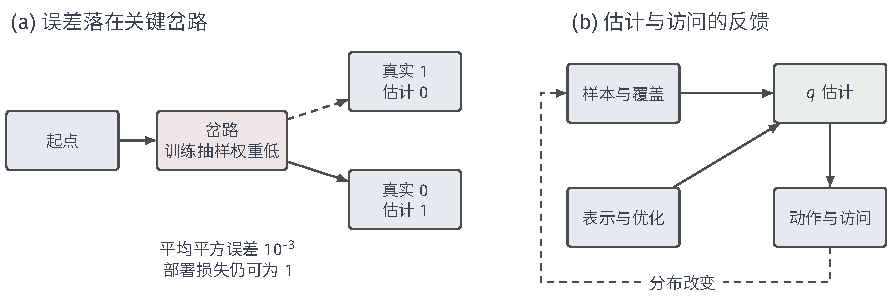
\includegraphics[width=150.887mm]{figures/10-reinforcement-learning/01-problems-and-solving/tikz/rl-learning-error-flow.pdf}
  \caption{局部错误与整体行为。左侧为人工指定的岔路反例，右侧区分表示、样本、优化及分布转移误差；图中的箭头是因果接口，不声称这些误差可以不加条件地线性相加。}
  \label{fig:rl-learning-error-flow}
\end{figure*}

表示误差决定函数类能否同时容纳关键区别，样本误差决定有限观测能否辨清回报，优化误差决定训练是否找到所要求的解；部署策略又可能访问训练中罕见的区域。这些环节必须分别检查。下一节改变主要优化对象，直接更新策略参数，但评论家误差与训练记录的覆盖不足并不会因此消失。

% Outline: 3.3
\section{无模型的策略优化}
\label{sec:rl-learning-policy}

连续控制力有无穷多取值，难以像表格动作那样逐个比较；即使只有上下左右，贪心动作也可能在估值稍有变化时突然切换。若希望直接调整控制输出或平滑改变动作概率，就可以参数化从状态到动作的映射，并按回报更新其参数。这称为\term{策略优化}（policy optimization）。无模型策略优化的更新不查询学得的动力学模型；价值估计器可以指导改变方向，却不负责预测环境转移。

这条路线的训练变量是策略参数，不要求先得到最优$Q$再作贪心选择。为估计更新方向，仍可配一个价值预测器：它为策略比较本次行动与通常回报，称为评论家；产生动作的策略称为行动者。先从不用评论家、只用采样回报的更新开始，随后再引入价值基线和两者的联合训练，这样可以分清价值预测承担的是辅助评价还是最终动作选择。

% Outline: 3.3.1
\subsection{策略梯度与回报梯度估计}
\label{sec:rl-learning-policy-gradient}

先考虑怎样从随机轨迹求出策略参数的上升方向。我们暂用有限状态动作和固定时域$H$，以便逐项对轨迹概率求导；策略$\pi_{\bm\theta,t}(a\mid s)$可依赖时间，在所讨论参数邻域内可微，并对合法动作严格为正。初始分布和环境核不依赖$\bm\theta$，奖励有界。记轨迹$\tau=(s_0,a_0,r_0,\ldots,s_H)$，用其折扣奖励和的期望比较候选参数，目标是增大$J_H$；$G_t^H$则保存动作$t$以后仍可影响的回报：
\begin{equation}
  J_H(\bm\theta)=\mathbb E_{\tau\sim P_{\mathcal E}^{\pi_{\bm\theta}}}
      \left[\sum_{t=0}^{H-1}\gamma^t r_t\right],
  \qquad
  G_t^{H}=\sum_{k=t}^{H-1}\gamma^{k-t}r_k .
  \label{eq:rl-learning-finite-policy-objective}
\end{equation}
策略的随机性提供了一个可求导的概率模型。无需知道某次动作怎样改变后继状态的导数，也能利用“这次轨迹的概率如何随参数变化”来估计回报梯度。

先把这种求导缩到一个单步两动作任务。设动作1奖励恒为$0.7$，动作2奖励恒为$0.4$，策略以$p=\sigma(\theta)=1/(1+e^{-\theta})$选择动作1。其期望回报为$J(\theta)=0.7p+0.4(1-p)$，直接求导得到$J'(\theta)=0.3p(1-p)$。如果不知道两个奖励，只能抽一个动作，仍可计算已选动作的对数概率导数：选动作1时为$1-p$，选动作2时为$-p$。把它乘实际奖励，平均得到
\[
 p\,0.7(1-p)+(1-p)\,0.4(-p)=0.3p(1-p).
\]
这个平均恰等于所需梯度，而一次样本只用到了策略概率和已观察奖励。对数概率的梯度称为得分函数（score function）；它说明当前参数变化会提高还是降低这次动作的发生概率。两种动作的样本方向可能相反，只有在抽样平均后才得到期望回报的上升方向。

推广到轨迹时，动作概率相乘，对数概率就相加；再用$\nabla p=p\nabla\log p$，可以把概率的导数写成“按原概率抽样后，对数梯度乘回报”的期望。这称为似然比估计，不需要对未知转移规律求导。下面的定理还会去掉每个动作之前已发生的奖励，因为这些奖励不能再受该动作影响。

\begin{theorem}[有限时域似然比策略梯度]
  \label{thm:rl-learning-likelihood-gradient}
  设状态空间$S$有限，每个非终止状态的合法动作集$\mathsf A(s)$有限且非空，$H\geq1$为整数，$0\leq\gamma\leq1$。初始分布及联合奖励转移核不依赖参数$\bm\theta$，奖励有界。在一个开参数邻域内，各$\pi_{\bm\theta,t}(\cdot\mid s)$均为合法动作上的严格正概率分布，且关于$\bm\theta$连续可微。用式\eqref{eq:rl-learning-finite-policy-objective}定义$J_H$和$G_t^H$。令
  $\bm z_t=\nabla_{\bm\theta}\log\pi_{\bm\theta,t}(a_t\mid s_t)$，则
  \begin{equation}
    \nabla_{\bm\theta}J_H
       =\mathbb E\left[
          \sum_{t=0}^{H-1}\gamma^t\bm{z}_tG_t^H\right].
    \label{eq:rl-learning-reward-to-go}
  \end{equation}
\end{theorem}
\begin{proof}
  轨迹分布分解为
  \[
    P_{\mathcal E}^{\pi_{\bm\theta}}(\mathrm d\tau)=\mu_0(s_0)
       \prod_{t=0}^{H-1}
       \pi_{\bm\theta,t}(a_t\mid s_t)
       p(\mathrm dr_t,s_{t+1}\mid s_t,a_t).
  \]
  环境项的导数为0，因此
  $\nabla P_{\mathcal E}^{\pi_{\bm\theta}}(\mathrm d\tau)
  =P_{\mathcal E}^{\pi_{\bm\theta}}(\mathrm d\tau)\sum_t\bm{z}_t$。
  该恒等式按测度理解，不要求奖励有离散点概率。有限状态动作和有限时域下，可以对策略概率的有限和逐项求导；随机奖励的有界性保证相应积分可交换。于是
  \[
    \nabla J_H
      =\mathbb E\left[
        \sum_{t=0}^{H-1}\bm{z}_t
        \sum_{k=0}^{H-1}\gamma^k r_k\right].
  \]
  令$I_t$为抽取$a_t$前的全部历史，则
  \[
    \mathbb E[\bm{z}_t\mid I_t]
       =\sum_a\pi_{\bm\theta,t}(a\mid s_t)
          \nabla\log\pi_{\bm\theta,t}(a\mid s_t)
       =\nabla\sum_a\pi_{\bm\theta,t}(a\mid s_t)=\bm0.
  \]
  当$k<t$时，$r_k$已经包含在$I_t$中，故
  $\mathbb E[\bm{z}_t r_k]=\bm0$。删去这些过去奖励，余下
  $\sum_{k=t}^{H-1}\gamma^k r_k=\gamma^tG_t^H$，即得结论。
\end{proof}

过去奖励的删除依据是得分函数对抽样前历史的条件均值为0；未来奖励前的时间权重并未消失。每个动作仍按$\gamma^t$计入起点目标。以$N$条独立同策略回合的
$N^{-1}\sum_{i,t}\gamma^t\bm{z}_{i,t}G_{i,t}^H$
作更新方向，就是一种REINFORCE估计。完整回报包含环境噪声与之后所有动作的随机性，因而无偏不等于低方差；但它不要求对环境转移求导\scite{rl1-williams1992-reinforce}

有限时域公式按时刻累加贡献。推广到无限折扣任务时，可以把这些访问概率汇总成一个状态分布，但需要先保证无限求和与求导可交换。采用平稳策略，并要求例如奖励与邻域内得分函数$\nabla\log\pi_{\bm\theta}$一致有界，就能对折扣级数及导数建立可积支配。再将给定状态动作的平均未来回报写成$Q^{\pi_{\bm\theta}}$，得到
\begin{equation}
  \nabla_{\bm\theta}J(\bm\theta)
    =\frac{1}{1-\gamma}
      \mathbb E_{\substack{s\sim d^{\pi_{\bm\theta}}\\
                           a\sim\pi_{\bm\theta}(\cdot\mid s)}}
        \left[\nabla_{\bm\theta}\log\pi_{\bm\theta}(a\mid s)
              Q^{\pi_{\bm\theta}}(s,a)\right].
  \label{eq:rl-learning-policy-gradient}
\end{equation}
这里$d^\pi$始终是归一化折扣占用分布，$J$始终是未归一化回报。若从固定长度回合中均匀抽时间步，却省去$\gamma^t$，所得权重通常不是$d^\pi$；调节学习率可以吸收整体常数，却不能修正不同时间步的相对权重。平均奖励目标、几何随机终止采样或特定工程近似各有自己的口径，不应把它们都称为式\eqref{eq:rl-learning-policy-gradient}的精确实现\scite{rl3-sutton2000policy}

归一化折扣占用可理解为一份带时间权重的访问记录：$d^\pi(s)=(1-\gamma)\sum_{t\geq0}\gamma^t\mathbb P_\pi(s_t=s)$。所有状态权重相加为1，所以它是概率分布；较早访问权重较大，较晚访问逐步折扣。策略梯度原来按时刻累加，改为从这份分布平均时，就要乘回$1/(1-\gamma)$。这个常数恢复总权重，不能将均匀时间抽样中各时刻相对权重的错误也一并修正。

表\ref{tab:rl-learning-policy-search-information}比较了三种改变策略的路径。确定性策略梯度将在后文展开；此处重要的是，参数可调并不意味着必须使用似然比，也不意味着能够穿过环境反向传播。

\begin{table*}[t]
  \centering
  \small
  \begin{tabularx}{\linewidth}{>{\raggedright\arraybackslash}p{29mm} >{\raggedright\arraybackslash}X >{\raggedright\arraybackslash}X}
    \toprule
    更新路径 & 所需奖励、概率或导数 & 不要求什么，以及主要代价 \\
    \midrule
    REINFORCE & 策略概率或密度及其对数梯度，采样回报 & 不求环境导数；长回合的梯度方差可能很大 \\
    确定性策略梯度 & 策略对参数的导数，$Q(s,a)$对动作的导数 & 不枚举连续动作；依赖评论家的动作方向导数 \\
    参数黑盒搜索 & 给定一组策略参数后可评估回报 & 不要求策略或环境可微；需支付多组参数的整轨迹评估成本 \\
    \bottomrule
  \end{tabularx}
  \caption{直接优化策略时的三类奖励、概率与导数需求。表中“无需模型导数”不等于“无需真实交互”。}
  \label{tab:rl-learning-policy-search-information}
\end{table*}

% Outline: 3.3.2
\subsection{基线、优势与方差控制}
\label{sec:rl-learning-baseline}

在本来就容易获得高回报的状态，许多动作都可能得到较大的$G_t$。直接以$G_t$加权，某次抽中的动作会因此获得很大更新，即使它没有优于其他动作；这些偶然更新可以在平均后相消，却增加了有限样本波动。\term{基线}（baseline）为回报设一个比较水平。若这个水平在本轮选动作之前已确定，减去它不会改变平均梯度，并可能去掉与本轮动作优劣无关的波动。

\begin{theorem}[动作抽样前基线的零均值性质]
  \label{thm:rl-learning-baseline}
  设$I_t$为抽取动作前的决策历史，其当前状态为$s_t$。在有限非空合法动作集$\mathsf A(s_t)$上，$a_t$按严格正、关于$\bm\theta$连续可微的概率分布$\pi_{\bm\theta,t}(\cdot\mid s_t)$抽取。设实基线$b_t$对$I_t$可测，且$b_t\nabla_{\bm\theta}\log\pi_{\bm\theta,t}(a_t\mid s_t)$可积。则
  \[
    \mathbb E[\nabla_{\bm\theta}
       \log\pi_{\bm\theta,t}(a_t\mid s_t)b_t]=\bm0.
  \]
  因而在式\eqref{eq:rl-learning-reward-to-go}中以$G_t^H-b_t$替换$G_t^H$，不改变期望梯度。
\end{theorem}
\begin{proof}
  条件于$I_t$，基线是常数，故
  \[
    \mathbb E[\bm{z}_t b_t\mid I_t]
      =b_t\sum_a\pi_{\bm\theta,t}(a\mid s_t)
                    \nabla\log\pi_{\bm\theta,t}(a\mid s_t)
      =b_t\nabla 1=\bm0.
  \]
  再对历史取期望，逐时刻相加即可。基线是否准确没有进入等式；进入等式的是它对本轮动作抽样的条件独立性。
\end{proof}

在单步两动作算例中，$p=1/2$时平均回报为$0.55$。取基线$0.55$，两个动作的超额回报为$0.15$和$-0.15$，对数梯度分别为$0.5$和$-0.5$，两种样本的乘积都为$0.075$。原来两个方向相反的样本，这时给出同一方向；平均梯度仍为$0.3(1/2)(1/2)=0.075$。这个确定性奖励例展示了基线如何去掉共同回报水平，不表示任意基线都能消除随机环境中的波动。

若以真实$V^\pi(s)$为基线，再按动作后的未来取平均，就得到优势$A^\pi(s,a)=Q^\pi(s,a)-V^\pi(s)$：它表示从同一状态出发，先选这个动作再按$\pi$继续，比立即按$\pi$选动作多得多少期望回报。优势大于0表示相对当前策略的平均水平更好，不要求动作回报本身为正；有步成本的网格中，一个负回报动作也可能具有正优势。

因此，用一个粗糙但预先固定的$V_{\bm w}(s_t)$减去完整回报，不会仅因价值误差而引入偏差。这里将基线作为停止求导的控制变量；若把$-\log\pi_{\bm\theta}(a_t\mid s_t)(G_t-b_{\bm\theta}(s_t))$当成普通损失并让梯度穿过$b_{\bm\theta}$，就多出不属于上述估计的项。同批动作被用于拟合基线后再评价这些动作时，拟合参数也可能随这次抽取的动作而变，需用独立批次、交叉拟合或相应分析恢复所需条件。

零均值性质允许许多基线，并没有指出哪一个最能减小方差。固定状态后，各动作的得分向量长度也会影响梯度波动，所以最小方差基线不总是$V^\pi(s)$。假定相关二阶矩有限且$\mathbb E[\lVert\bm z\rVert^2\mid s]>0$；由于基线不改变梯度均值，最小化其方差等价于在实数$b$上最小化向量估计的二阶矩
$\mathbb E[\lVert\bm z\rVert^2(G-b)^2\mid s]$，对$b$求导可得
\[
  b_*(s)=
    \frac{\mathbb E[\lVert\bm z\rVert^2G\mid s]}
         {\mathbb E[\lVert\bm z\rVert^2\mid s]}.
\]
若分母为0，则给定该状态时$\bm z$几乎处处为零，任意有限基线对梯度的贡献都相同，无须使用这个比值。分母为正时，只有得分长度对回报的加权不改变条件均值等额外条件成立，$b_*(s)$才等于$V^\pi(s)$。实践仍常用价值基线，是因为它可学习、易复用，并直接给出优势$A^\pi=Q^\pi-V^\pi$的解释。

上述基线论证仍使用完整回报。如果需要在远处奖励出现前更新，就必须让价值预测替代未观察的未来，这会增加自举依赖。我们先把多步回报减去当前状态基线，得到多步优势估计；它评价本次动作比状态的一般水平多带来多少回报。给定长度$L$的片段，暂时冻结$V_{\bm w}$，令
\[
  \delta_{t+l}=r_{t+l}+\gamma V_{\bm w}(s_{t+l+1})
                            -V_{\bm w}(s_{t+l}),\qquad
  \widehat A_t^{[n]}=\sum_{l=0}^{n-1}\gamma^l\delta_{t+l}.
\]
相邻价值项抵消，故$\widehat A_t^{[n]}=G_t^{[n]}-V_{\bm w}(s_t)$，方括号仍表示回报长度。\term{广义优势估计}（generalized advantage estimation, GAE）把不同长度的优势作几何混合：
\begin{align}
  \widehat A_t^{\mathrm{GAE}}
    &=(1-\lambda)\sum_{n=1}^{L-1}\lambda^{n-1}\widehat A_t^{[n]}
       +\lambda^{L-1}\widehat A_t^{[L]}
       \notag\\
    &=\sum_{l=0}^{L-1}(\gamma\lambda)^l\delta_{t+l},
       \qquad 0\leq\lambda\leq1.
    \label{eq:rl-learning-gae}
\end{align}
第二个等式来自对每个$\delta_{t+l}$汇总其在所有$n>l$中的权重，系数恰为$\gamma^l\lambda^l$。最后一项的特殊权重保留了有限片段末端的全部剩余质量，不能直接丢掉。

图\ref{fig:rl-learning-gae}给出三个TD误差的教学计算。取$\gamma=0.9$、$\lambda=0.8$，误差与加权结果为
\[
  (\delta_t,\delta_{t+1},\delta_{t+2})=(0.2,-0.1,0.5),\qquad
  \widehat A_t=0.3872.
\]
其中$0.3872=0.2-0.72(0.1)+0.5184(0.5)$。
从后往前递推$\widehat A_j=\delta_j+\gamma\lambda\widehat A_{j+1}$即可线性时间计算整段优势。记片段结束时刻为$T=t+L$，先令优势累积器$\widehat A_T=0$，再从$j=T-1$递推到$t$。非终止的批次边界仍保留$V_{\bm w}(s_T)$，但它只进入最后一个TD误差$\delta_{T-1}$，不能再用来初始化$\widehat A_T$；真正终止时则令该末端状态价值为0。片段不跨越回合重置，不能把下一回合的优势传回上一回合。

\begin{figure}[htbp]
  \centering
  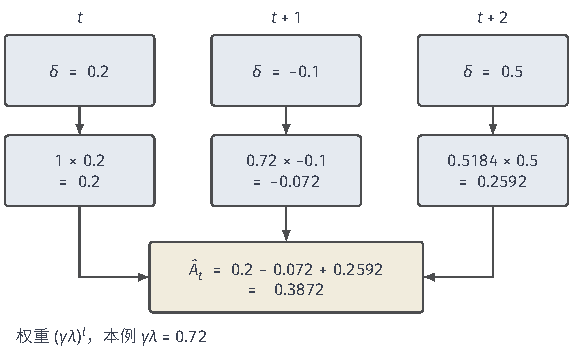
\includegraphics[width=96.961mm]{figures/10-reinforcement-learning/01-problems-and-solving/tikz/rl-learning-gae.pdf}
  \caption{GAE的几何加权。每列是一项TD误差及其对当前优势的贡献；数值是人工指定的三步算例，不是实验学习曲线。}
  \label{fig:rl-learning-gae}
\end{figure}

若评论家等于$V^\pi$，后继TD误差在其动作抽样前历史下均值为0；因此在同策略条件下，对任意$\lambda$，上式给定$(s_t,a_t)$的条件均值均为$A^\pi(s_t,a_t)$。近似评论家则不同。令$e=V_{\bm w}-V^\pi$，在无限折扣和有界误差下，近似GAE相对精确GAE的条件均值变化为
\[
  -e(s_t)+
  \gamma(1-\lambda)\,
  \mathbb E\left[
     \sum_{l=1}^{\infty}(\gamma\lambda)^{l-1}e(s_{t+l})
        \,\middle|\,s_t,a_t\right].
\]
第一项仍是状态基线，乘得分函数后均值为0；第二项通常依赖所选动作，会改变策略更新。$\lambda=1$且完整终止回报可用时，这个自举误差项消失；若仅有截断片段，还留有末端价值误差。表\ref{tab:rl-learning-baseline-bootstrap}将两种评论家用途并排，避免把控制变量的无偏结论错误搬到所有自举目标上\scite{rl3-schulman2016gae}

\begin{table*}[t]
  \centering
  \small
  \begin{tabularx}{\linewidth}{>{\raggedright\arraybackslash}p{30mm} >{\raggedright\arraybackslash}X >{\raggedright\arraybackslash}X}
    \toprule
    评论家的位置 & 估计示例 & 偏差和方差应怎样判断 \\
    \midrule
    状态基线 & 完整$G_t-V_{\bm w}(s_t)$ & 动作抽样前固定即可保持期望；误差影响方差，不保证一定降方差 \\
    未来回报替代 & $r_t+\gamma V_{\bm w}(s_{t+1})-V_{\bm w}(s_t)$ & 后继误差可随动作变化，通常产生自举偏差 \\
    多步混合 & 式\eqref{eq:rl-learning-gae} & $\lambda$和片段长度共同控制自举依赖与随机回报范围 \\
    同批拟合再复用 & 用该动作的回报训练基线并立即扣减 & 必须重新检查条件独立、旧策略比率与重复优化造成的分布变化 \\
    \bottomrule
  \end{tabularx}
  \caption{减去一个数，与用一个数替代尚未观察的未来，是不同操作。}
  \label{tab:rl-learning-baseline-bootstrap}
\end{table*}

% Outline: 3.3.3
\subsection{自然梯度、信赖域与近端更新}
\label{sec:rl-learning-trust-region}

梯度给出方向，步长还需反映动作分布会改变多少。参数距离本身不能提供统一尺度：二动作策略写成$p=\sigma(\theta)$时，$\theta$从0增至$0.1$，$p$约增至$0.5250$；同一策略族改用$\phi=10\theta$，让$\phi$增加$0.1$，$p$却只增至约$0.5025$。相同坐标步长产生了不同的行为变化，因此需要直接用新旧动作分布的差异衡量更新。

令旧参数为$\bm\theta$、候选新参数为$\bm\theta+\bm\Delta$。我们用KL散度比较每个状态的新旧动作分布，并按旧策略占用分布平均，使本次局部比较的状态权重固定。设$S$和合法动作集有限，旧占用$d^\pi$在本次比较中固定，各合法动作概率在开参数邻域内严格为正且二阶连续可微。概率归一化使KL在$\bm\Delta=0$处的一阶项为0，二阶展开为
\begin{align}
  \mathbb E_{d^\pi}\!
    \left[D_{\mathrm{KL}}
       (\pi_{\bm\theta}(\cdot\mid s)
           \Vert\pi_{\bm\theta+\bm\Delta}(\cdot\mid s))\right]
    &=\tfrac12\bm\Delta^\top\bm F\bm\Delta
         +o(\lVert\bm\Delta\rVert^2), \notag\\
  \bm F&=\mathbb E_{d^\pi,\pi}[\bm z\bm z^\top].
  \label{eq:rl-learning-fisher}
\end{align}
一次项因概率归一化而消失；二次项$\bm F$是Fisher信息矩阵，衡量参数变化在动作分布中留下多大痕迹。\term{自然梯度}用这个局部度量而不是坐标长度比较方向。设$\bm g=\nabla J$在有效子空间内非零、$\bm F$在该子空间正定且$\delta>0$，则
\[
  \argmax_{\bm\Delta:\,\bm\Delta^\top\bm F\bm\Delta/2\leq\delta}
       \bm g^\top\bm\Delta
     =
     \sqrt{\frac{2\delta}{\bm g^\top\bm F^{-1}\bm g}}\,
       \bm F^{-1}\bm g.
\]
若$\bm g=\bm0$，局部线性目标没有偏好的上升方向，可取零步；上述归一化公式不适用。若参数冗余导致$\bm F$奇异，应限制到可辨识子空间、使用伪逆，或明确采用$\bm F+\xi\bm I$的阻尼近似。自然梯度的坐标不变性是局部几何性质，不是任意有限步长的回报保证\scite{rl3-kakade2002natural}

自然梯度的约束可以看成给行为变化设置预算。普通梯度在一个参数欧氏球内寻找回报线性近似最大的方向；这里改用$\bm\Delta^\top\bm F\bm\Delta/2\leq\delta$这个椭球，让同样的KL预算可以在不敏感的参数方向走得远一些，在很敏感的方向走得近一些。解椭球内的线性最大化，才得到$\bm F^{-1}\bm g$，而不是因为矩阵可逆就任意将梯度乘一个逆矩阵。它只解释一次局部选择，实际有限步仍要核对动作分布和回报。

局部分布距离说明如何计量一步，却还没有保证回报会上升。要判断改进，需将新策略的回报差写成可评价的优势。下面的恒等式表明：应平均的是新策略实际访问状态上的旧策略优势，不能任意用旧策略轨迹的抽样分布替换。

\begin{theorem}[折扣性能差恒等式]
  \label{thm:rl-learning-performance-difference}
  设$S$有限，各非终止状态的合法动作集有限且非空，奖励有界，$0\leq\gamma<1$。两个平稳策略$\pi,\pi'$使用同一环境核和同一初始分布$\mu_0$，$d^{\pi'}$为其归一化折扣占用分布，$A^\pi=Q^\pi-V^\pi$。则
  \begin{equation}
    J(\pi')-J(\pi)
       =\frac{1}{1-\gamma}
          \mathbb E_{s\sim d^{\pi'},\,a\sim\pi'}[A^\pi(s,a)].
    \label{eq:rl-learning-performance-difference}
  \end{equation}
\end{theorem}
\begin{proof}
  沿$\pi'$的轨迹，条件期望给出
  $A^\pi(s_t,a_t)
    =\mathbb E[r_t+\gamma V^\pi(s_{t+1})-V^\pi(s_t)
                \mid s_t,a_t]$。乘$\gamma^t$并求和到$n-1$，
  \[
    \mathbb E_{\pi'}\sum_{t=0}^{n-1}\gamma^t A^\pi(s_t,a_t)
      =\mathbb E_{\pi'}\sum_{t=0}^{n-1}\gamma^t r_t
         -\mathbb E_{\mu_0}V^\pi(s_0)
         +\gamma^n\mathbb E_{\pi'}V^\pi(s_n).
  \]
  $V^\pi$有界使尾项趋于0，前两项趋于$J(\pi')-J(\pi)$。按归一化占用分布的定义，左边极限等于
  $(1-\gamma)^{-1}\mathbb E_{d^{\pi'},\pi'}A^\pi$。
\end{proof}

更新前尚未收集新策略轨迹，直接计算$d^{\pi'}$下的优势仍有困难。用$d^\pi$替代它，就得到一个可由旧策略轨迹样本估计的局部代理目标；代理提高到什么程度能支持真实改进，还要控制这项替代误差。若连动作也用旧策略样本估计，还需$\pi'(\cdot\mid s)\ll\pi(\cdot\mid s)$，即新策略所选动作在旧策略下有正概率。此时动作比率给出
\[
  \mathcal L_\pi(\pi')
    =J(\pi)+\frac1{1-\gamma}
         \mathbb E_{d^\pi,\,a\sim\pi}
           \left[\frac{\pi'(a\mid s)}{\pi(a\mid s)}
                         A^\pi(s,a)\right].
\]
动作比率校正了同一状态的动作分布，却没有校正状态访问分布。要界住这项变化，使用总变差（total variation, TV）：对离散动作分布$p,q$，
$\operatorname{TV}(p,q)=\tfrac12\sum_a|p(a)-q(a)|
=\tfrac12\lVert p-q\rVert_1$，
其中动作在同一合法域上比较。它也等于$\sup_B|p(B)-q(B)|$，即允许动作事件$B$上概率差的最大值；这个事件定义同样适用于连续分布。令
$\eta=\max_s\operatorname{TV}(\pi'(\cdot\mid s),\pi(\cdot\mid s))$、
$\epsilon_A=\max_{s,a}|A^\pi(s,a)|$。同一转移核按两份动作分布混合时，不放大其$L^1$差，故单步状态转移差至多为$2\eta$；再将占用流方程中的后续传播按折扣累加，可得
$\lVert d^{\pi'}-d^\pi\rVert_1\leq2\gamma\eta/(1-\gamma)$；
又因$\mathbb E_\pi A^\pi=0$，
$|\mathbb E_{\pi'}A^\pi(s,\cdot)|\leq2\epsilon_A\eta$。两式相乘得到
\begin{equation}
  J(\pi')\geq\mathcal L_\pi(\pi')
       -\frac{4\gamma\epsilon_A}{(1-\gamma)^2}\eta^2 .
  \label{eq:rl-learning-trpo-bound}
\end{equation}
这里$\eta$取全部状态上动作分布总变差的最大值，因为少见状态的策略变化也可能改变后续可达区域；仅按旧访问分布平均，可能漏掉这种变化。由Pinsker不等式，可进一步用最大状态KL控制$\eta^2$。因此，下界要求的不只是提高旧策略轨迹样本上的代理，还要限制所有状态的新旧策略差异，使状态分布替代的损失不足以抵消提升。

信赖域策略优化（trust region policy optimization, TRPO）的理论分析从此类下界出发，实践实现则用样本平均KL约束、共轭梯度近似Fisher逆乘积和回溯线搜索，以有限计算求一个局部步。平均KL不控制所有少见状态，估计优势也不等于真实优势，因此“精确下界提高”与“实践TRPO更新”不能无条件互换。兼容函数逼近给出了另一条严格但受限的连接：若评论家为
$f_{\bm w}(s,a)=\bm z(s,a)^\top\bm w$，并在同一$d^\pi\pi$下精确最小化
$\mathbb E[(Q^\pi-b(s)-f_{\bm w})^2]$，
正规方程给出$\mathbb E[\bm z(Q^\pi-b-f_{\bm w})]=0$，从而
$\nabla J=\bm F\bm w/(1-\gamma)$。这要求特征兼容、正确加权和评价解足够准确，不是任意价值网络都保留梯度方向\scite{rl3-schulman2015trpo,rl3-agarwal2021policygradient}

TRPO的约束求解需要额外计算。近端策略优化（proximal policy optimization, PPO）改为优化一个可用于小批量更新的代理，限制过度改变动作概率后还能从同一样本获取多少收益。记旧策略为$\pi_{\mathrm{old}}$，
$q_t(\bm\theta)=\pi_{\bm\theta}(a_t\mid s_t)/
\pi_{\mathrm{old}}(a_t\mid s_t)$，优势在本轮优化中固定。

概率比$q_t$先回答这条旧样本在新策略下应占多少动作权重。例如旧概率为$0.2$，新概率为$0.3$，比率为$1.5$。若优势为正，这份代理鼓励继续增大它；但旧样本没有验证新策略大幅改变后会访问哪里。裁剪目标因此让这条样本在有利方向上的收益到阈值后停止增长，减少继续靠同一条证据推动过大变化的动机。它裁剪的是目标贡献，参数仍由全部样本共同更新。PPO-Clip据此最大化
\begin{equation}
  L^{\mathrm{clip}}(\bm\theta)=
    \widehat{\mathbb E}_t
      \left[\min\left\{q_t\widehat A_t,\,
        \operatorname{clip}(q_t,1-\varepsilon,1+\varepsilon)
                      \widehat A_t\right\}\right].
  \label{eq:rl-learning-ppo-clip}
\end{equation}
这里$\widehat{\mathbb E}_t$使用明确选定的批次权重；若要对应前述折扣代理，权重应匹配$d^{\pi_{\mathrm{old}}}$，均匀抽时间步未必满足。内部最小值是在未裁剪和裁剪后的两项贡献中取较小者，使过大的有利概率变化不再增加代理收益：$\widehat A_t>0$时，$q_t>1+\varepsilon$进入平坦区；$\widehat A_t<0$时，$q_t<1-\varepsilon$进入平坦区。反方向变化仍受惩罚。外层则对策略参数最大化这个批次目标。图\ref{fig:rl-learning-policy-geometry}展示两种优势符号下的曲线，并与参数化例子对照。

\begin{figure*}[t]
  \centering
  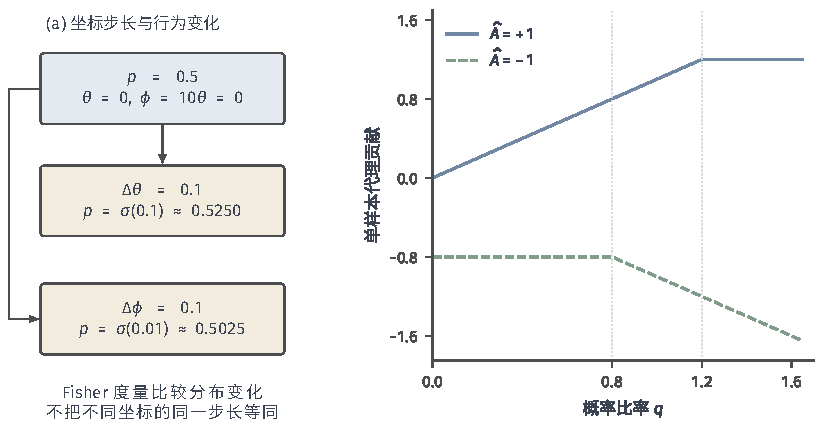
\includegraphics[width=139.587mm]{figures/10-reinforcement-learning/01-problems-and-solving/tikz/rl-learning-policy-geometry.pdf}
  \caption{参数距离、分布距离与PPO裁剪。左侧为同一Bernoulli策略的两种坐标；右侧为$\varepsilon=0.2$、$\widehat A=\pm1$时式\eqref{eq:rl-learning-ppo-clip}的解析折线，裁剪后的平坦区不表示概率比被硬性截住。}
  \label{fig:rl-learning-policy-geometry}
\end{figure*}

例如正优势为1、概率比从1.2变到1.5，单样本贡献仍为1.2；但共享参数受其他样本影响，仍可能继续推动这个比率。PPO-KL改用
$\widehat{\mathbb E}[q_t\widehat A_t]
-\eta_{\mathrm{KL}}\widehat{\mathbb E}_sD_{\mathrm{KL}}
(\pi_{\mathrm{old}}\Vert\pi_{\bm\theta})$
并调节惩罚系数，两者都需要监控实际策略变化。算法\ref{alg:rl-learning-ppo}给出一次完整的交互采样与训练样本复用循环；工程上常加熵项、优势标准化、梯度裁剪与KL提前停止，应分别记录，不能混作裁剪目标的数学性质\scite{rl3-schulman2017ppo}

\begin{algorithm}[一轮PPO-Clip：采样、固定目标与近端优化]
  \label{alg:rl-learning-ppo}
  \begin{algorithmic}[1]
    \State 保存$\bm\theta_{\mathrm{old}}\gets\bm\theta$，冻结旧策略与本轮用于估计优势的评论家。
    \State 用$\pi_{\mathrm{old}}$收集片段，记录状态、动作、$r_t$、真实终止标记、截断标记和旧对数概率。
    \State 真实终止处置末端价值为0；非终止片段边界使用冻结评论家的末端预测。
    \State 从后向前计算式\eqref{eq:rl-learning-gae}，固定$\widehat A_t$与价值目标$\widehat R_t=\widehat A_t+V_{\mathrm{old}}(s_t)$。
    \For{预先指定的$E$轮小批量优化}
      \State 从本轮旧策略采集的训练片段取批次，按已声明权重计算$q_t$与$L^{\mathrm{clip}}$。
      \State 行动者对$L^{\mathrm{clip}}$做梯度上升；评论家对$(V_{\bm w}(s_t)-\widehat R_t)^2$做下降。
      \State 测量旧新策略KL；若采用提前停止规则且超过阈值，停止本轮行动者更新。
    \EndFor
    \State 丢弃本轮作为近端优化依据的旧轨迹批次，使用新策略开始下一轮真实采样。
  \end{algorithmic}
\end{algorithm}

多轮优化复用的是同一个旧分布上的代理，不是每轮都重新获得同策略无偏梯度。理论单调改进是关于特定精确下界和约束的结论；局部平稳性是优化算法的另一类结论；表格softmax等特殊参数化下的全局分析又要求另外的条件。一般神经网络PPO不能从名称中的“近端”继承这三种保证。

\paragraph{小梯度与精确表格保证}
\label{sec:rl-learning-tabular-policy-optimization}
即使梯度完全准确，它很小也未必说明策略已经近优。另设一个单步两动作任务，好动作奖励1、坏动作奖励0，以$p=\sigma(\theta)$表示好动作概率，则$J(\theta)=p$、$J'(\theta)=p(1-p)$。当$p=10^{-6}$时，梯度约为$10^{-6}$，策略离最优回报却仍差$1-10^{-6}$。梯度被罕见动作的概率压小了；多步任务中，很少访问关键状态也会压小相应参数的梯度。因此，普通参数梯度的长度不能单独作为策略损失证书。

自然策略梯度（natural policy gradient, NPG）用Fisher几何调整这些方向的尺度。单步例的Fisher信息为$p(1-p)$，故其逆乘精确梯度得到方向1，而不是随$p$一同趋近零。要把这种局部解释连到一般MDP中的正面结论，可以采用完全表格化、每轮精确评价的设定。以下结论固定同一个初始分布来计算梯度和比较性能，不使用回放分布替代。

\begin{theorem}[精确表格自然策略梯度的全局进展]
  \label{thm:rl-learning-tabular-npg}
  设$S$为非空有限状态集，所有状态共享非空有限动作集$\mathsf A$，$n_A=|\mathsf A|$，环境核时间齐次，奖励为确定性函数$R(s,a)\in[0,1]$，且$0<\gamma<1$。固定初始分布$\mu_0$，并只保留从$\mu_0$出发在某个合法策略下可达的状态，$\pi^*$为该MDP的最优平稳策略。令
  $J(\pi)=\mathbb E_{s_0\sim\mu_0}V^\pi(s_0)$，
  策略按独立状态动作参数作softmax参数化：
  $\pi_{\bm\theta}(a\mid s)=
  e^{\theta_{s,a}}/\sum_b e^{\theta_{s,b}}$。
  记$\pi^{(k)}=\pi_{\bm\theta^{(k)}}$。从$\bm\theta^{(0)}=\bm0$开始，取任意固定步长$\eta>0$。每轮精确计算当前策略的价值、优势、梯度和式\eqref{eq:rl-learning-fisher}中按$d^{\pi_{\bm\theta}}$加权的Fisher矩阵$\bm F(\bm\theta)$，并更新
  $\bm\theta^{(k+1)}=\bm\theta^{(k)}+
  \eta\bm F(\bm\theta^{(k)})^\dagger
          \nabla_{\bm\theta}J(\pi_{\bm\theta})$，其中导数在$\bm\theta^{(k)}$处计算。
  这里$\dagger$为Moore--Penrose伪逆。其诱导策略满足
  \begin{equation}
    \begin{aligned}
    \pi^{(k+1)}(a\mid s)&=
    \frac{\pi^{(k)}(a\mid s)
      \exp\!\left(\eta A^{\pi^{(k)}}(s,a)/(1-\gamma)\right)}
    {Z_k(s)},\\
    Z_k(s)&=\sum_b\pi^{(k)}(b\mid s)
      \exp\!\left(\eta A^{\pi^{(k)}}(s,b)/(1-\gamma)\right),
    \end{aligned}
    \label{eq:rl-learning-tabular-npg-step}
  \end{equation}
  且对每个整数$k\geq1$，
  \begin{equation}
    J(\pi^*)-J(\pi^{(k)})
       \leq\frac{\log n_A}{\eta k}
            +\frac{1}{(1-\gamma)^2k}.
    \label{eq:rl-learning-tabular-npg-rate}
  \end{equation}
\end{theorem}

表格softmax的精确梯度中含有
$d^\pi(s)\pi(a\mid s)A^\pi(s,a)/(1-\gamma)$。
Fisher伪逆在可辨识方向上抵消访问和动作概率带来的尺度，得到式\eqref{eq:rl-learning-tabular-npg-step}；softmax对同一状态的全部参数加相同常数不改变策略，所以使用伪逆不要求冗余参数下的Fisher可逆。在动作分布中，这相当于以旧策略作参考，按当前优势指数加权；第\ref{sec:rl-learning-regularized-search}节将从KL正则的局部优化解释这种形式。

这一更新的进展可以由两个有限量控制。旧策略的平均优势为0，指数的凸性给出$\log Z_k(s)\geq0$；新策略的平均优势则为
$\mathbb E_{\pi^{(k+1)}}A^{\pi^{(k)}}
=(1-\gamma)[D_{\mathrm{KL}}(\pi^{(k+1)}\Vert\pi^{(k)})+\log Z_k(s)]/\eta\geq0$。
性能差恒等式因此给出逐状态价值不下降。对固定最优策略$\pi^*$，更新式还给出
\[
 \frac{\eta}{1-\gamma}
       \mathbb E_{a\sim\pi^*}A^{\pi^{(k)}}(s,a)
 =D_{\mathrm{KL}}(\pi^*\Vert\pi^{(k)})
  -D_{\mathrm{KL}}(\pi^*\Vert\pi^{(k+1)})+\log Z_k(s),
\]
其中各动作分布都条件于同一$s$。按最优策略占用平均并对轮次求和，前两项望远镜相消；均匀初值使剩余初始KL不超过$\log n_A$。从$s$出发的新策略折扣占用在$s$至少有初始质量$1-\gamma$，结合刚才的非负平均优势，又有
$\log Z_k(s)\leq
\eta[V^{\pi^{(k+1)}}(s)-V^{\pi^{(k)}}(s)]/(1-\gamma)$。
故归一化项也可按轮次累加为价值增长，而$[0,1]$奖励使价值范围至多为$1/(1-\gamma)$。再用最后一轮的损失不超过各轮平均，便得到式\eqref{eq:rl-learning-tabular-npg-rate}。该定理及完整分析见Agarwal等的上述研究。

这给出了参数目标虽非凹、特定策略更新仍能趋近全局最优的实例。式中的$k$计精确优化轮次：每轮仍须取得精确价值与梯度，不能将$k$当作真实交互样本数。函数逼近、抽样误差、不同初始分布和PPO裁剪改变了推导条件，需要分别重新控制；Fisher几何本身没有消除这些困难。

% Outline: 3.3.4
\subsection{行动者—评论家的评价—改进耦合}
\label{sec:rl-learning-actor-critic}

前面已用价值基线和优势帮助计算策略更新；实际训练还需要随策略变化不断重学这些评价量。\term{行动者—评论家}（actor--critic）将两个过程耦合：行动者是产生动作的参数策略，评论家是为其更新估计价值或优势的函数。最终目标仍是改进策略，而不是分别追求两个不相关的数值。行动者改变后，评论家的目标策略及后续样本分布也改变，因此必须检查两个更新能否相互跟踪。

对同策略的一步经验，先用奖励和后继估值构造TD误差；评论家据此修正当前价值，行动者则把这个误差当作本次动作的优势。为了与折扣起点目标一致，行动者贡献仍保留$\gamma^t$。一种最简单的联合更新为
\begin{align}
  \delta_t&=r_t+\gamma(1-z_t)V_{\bm w}(s_{t+1})-V_{\bm w}(s_t),
       \notag\\
  \bm w&\gets\bm w+\alpha_t^V\delta_t\nabla_{\bm w}V_{\bm w}(s_t),
       \notag\\
  \bm\theta&\gets\bm\theta+
       \alpha_t\gamma^t\delta_t
          \nabla_{\bm\theta}\log\pi_{\bm\theta}(a_t\mid s_t).
  \label{eq:rl-learning-one-step-ac}
\end{align}
$z_t$仅表示真实终止；若按$d^\pi$直接抽样状态动作，则可把最后一行改写成含$1/(1-\gamma)$的占用分布梯度口径。这里保留回合时间权重，是为了与本章的$J$一致。评论家采用半梯度，行动者把$\delta_t$当成停止求导的优势估计，两个梯度不能混在一起。多步行动者—评论家用$n$步优势或GAE替换$\delta_t$；资格迹则把更新沿过去状态动作传播。

\begin{example}[同一经验的两种更新]
  \label{ex:rl-learning-actor-critic}
  在基准网格起点$(1,1)$，两个合法意图动作是向右和向上。假设当前评论家估计
  $V(1,1)=0.2$、$V(2,1)=0.5$，策略以
  $p_{\text{右}}=\sigma(\theta)$、$\theta=0$表示，均为本次手算指定的初值。第一步选右且实际到达$(2,1)$，得到$r_0=-0.04$，于是
  $\delta_0=-0.04+0.9(0.5)-0.2=0.21$。
  取评论家步长$0.1$，表格状态值更新为$0.221$；取行动者步长$0.2$，因
  $\partial_\theta\log p_{\text{右}}=1-p_{\text{右}}=0.5$，
  $\theta$更新为$0.021$，向右概率变为约$0.50525$。前者提高当前状态的估值，后者提高相对于当前基线表现较好的动作概率；两者不在拟合同一个数。
\end{example}

图\ref{fig:rl-learning-actor-critic}中的两条反馈路径解释了耦合来源。评论家的价值估计会改变行动者的训练目标，行动者又会改变评论家以后看见的样本。即使一次评论家回归收敛，也不代表整个反馈过程已经稳定。

\begin{figure*}[t]
  \centering
  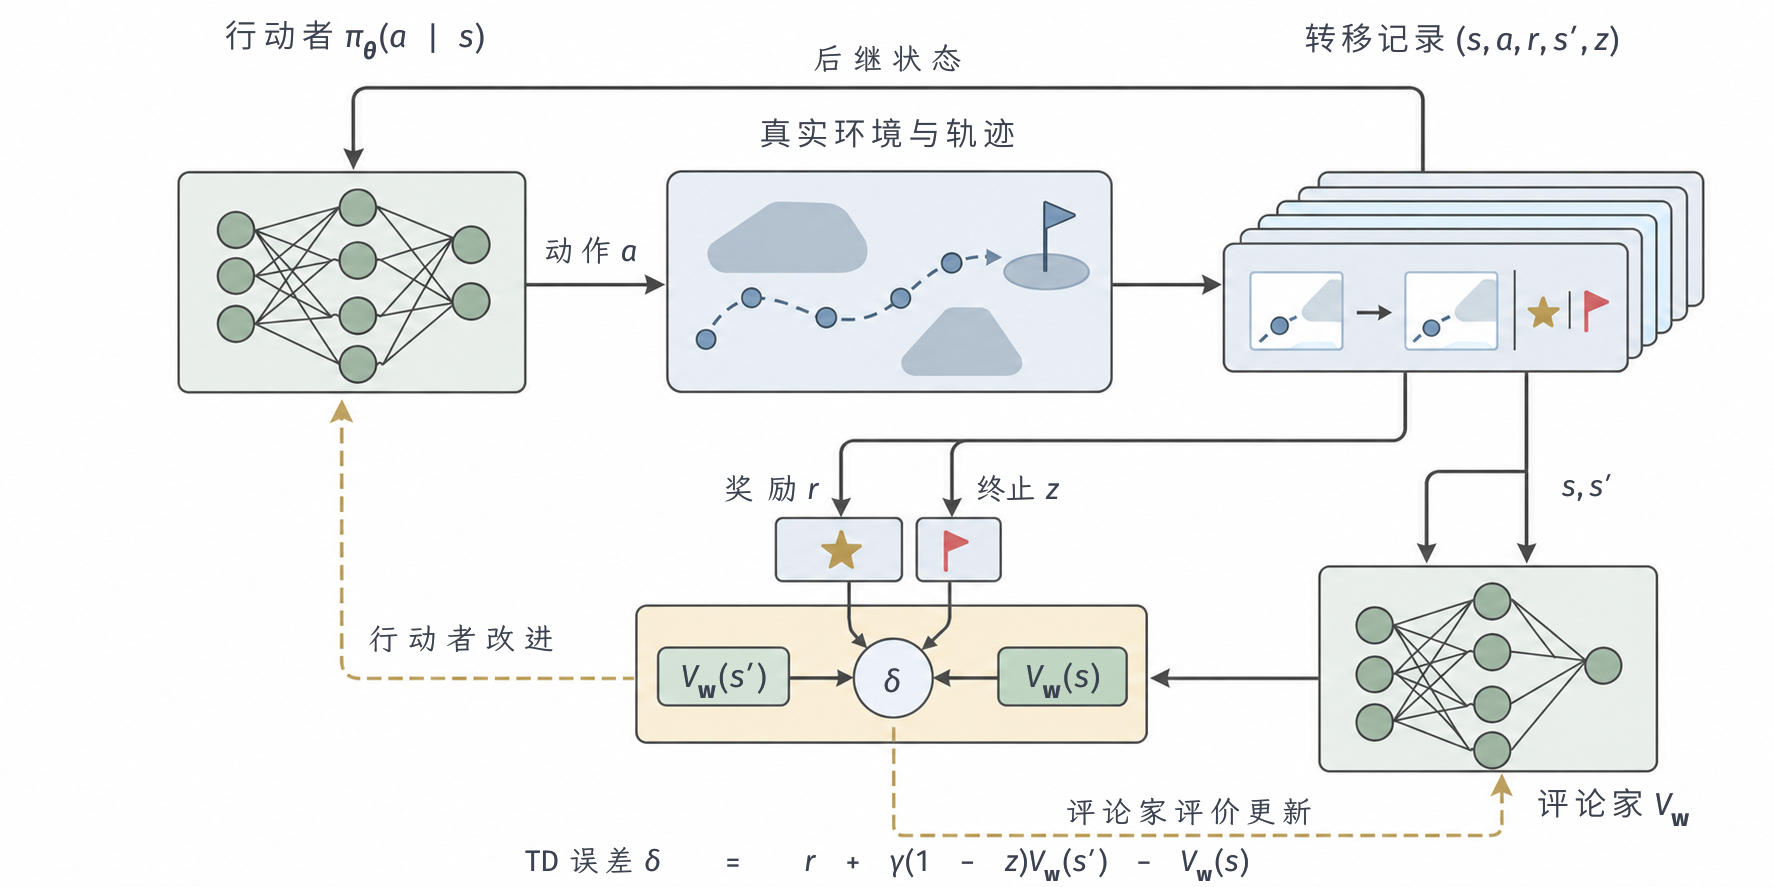
\includegraphics[width=157.400mm]{figures/10-reinforcement-learning/01-problems-and-solving/generated/rl-learning-actor-critic/figure.png}
  \caption{行动者—评论家的共享转移记录与两条更新路径。实线表示采样和价值估计，黄色虚线分别更新行动者与评论家；评论家估计的是价值。轨迹与神经节点仅为机制示意，不表示固定网络结构或轨迹长度。}
  \label{fig:rl-learning-actor-critic}
\end{figure*}

\Needspace{14\baselineskip}
A2C常把多个采样器在同一组参数下收集的短片段同步汇总再更新；A3C则允许采样器异步贡献梯度\scite{rl3-mnih2016asynchronous}
表\ref{tab:rl-learning-ac-interfaces}把这一区别落实到目标对应的轨迹采样条件。异步减少等待，不会让旧参数产生的动作自动变成当前策略动作。

\begin{table*}[t]
  \centering
  \small
  \begin{tabularx}{\linewidth}{>{\raggedright\arraybackslash}p{21mm} >{\raggedright\arraybackslash}X >{\raggedright\arraybackslash}X}
    \toprule
    接口 & 轨迹采样与更新时机 & 需要检查的条件 \\
    \midrule
    一步AC & 一次转移后更新价值与策略 & TD自举误差、步长、样本权重 \\
    A2C & 多环境短片段同步形成一个更新批次 & 批次内策略版本和终止处理一致；并行仅改变采样组织 \\
    A3C & 工作进程使用局部参数采样，异步提交梯度 & 参数滞后与更新冲突；当前全局参数下通常已非严格同策略 \\
    带GAE的AC & 冻结评价器构造片段优势，再更新策略 & $\lambda$、末端自举与估计器是否固定；重复批次优化另需分布处理 \\
    \bottomrule
  \end{tabularx}
  \caption{行动者—评论家的轨迹采样接口。同步、异步与优势长度是可以组合的不同维度。}
  \label{tab:rl-learning-ac-interfaces}
\end{table*}

经典双时间尺度分析让评论家比行动者变化得快。若评论家步长为$\alpha_t^V$、行动者为$\alpha_t$，典型要求为两者的和发散、平方和收敛，并有$\alpha_t/\alpha_t^V\to0$。再加上适用的遍历性、平滑性、参数有界性以及评论家在固定策略下存在稳定且可跟踪的解，快速过程可近似看成已经评价了当前策略，慢速过程才接近一个策略改进常微分方程。线性或兼容评论家等参数化条件决定这个方程是否为真正梯度场；非凸参数化的结果通常也只是局部或驻点性质。固定大步长、任意共享深度网络及不受控参数滞后均不由这条证明路线覆盖\scite{rl3-konda2000actor}

% Outline: 3.3.5
\subsection{连续动作、离策略与最大熵更新}
\label{sec:rl-learning-continuous-soft}

连续动作无法逐个比较，但若评论家能给出动作附近的价值变化，就可以沿价值上升方向调整行动者输出。令确定性行动者为$a=f_{\bm\theta}(s)$，其诱导策略为$\pi_{\bm\theta}$。确定性策略梯度（deterministic policy gradient, DPG）先求$Q$对动作的导数，再通过行动者传到参数；若所需函数可微、导数可积，则
\begin{equation}
  \nabla_{\bm\theta}J
    =\frac1{1-\gamma}
       \mathbb E_{s\sim d^{\pi_{\bm\theta}}}
       \left[
         (\nabla_{\bm\theta}f_{\bm\theta}(s))^\top
         \left.\nabla_a Q^{\pi_{\bm\theta}}(s,a)
                    \right|_{a=f_{\bm\theta}(s)}
       \right].
  \label{eq:rl-learning-dpg}
\end{equation}
行动者沿评论家认为价值上升的动作方向移动，再用链式法则把这个方向传到参数。环境仍不必可微，但评论家的动作导数必须有意义；动作上的函数值误差小，也不保证动作导数准确\scite{rl3-silver2014dpg}

动作方向导数可在一个局部教学评论家上观察。固定状态，令$Q(s,a)=-(a-0.6)^2$、行动者输出$a=\theta$。当前$\theta=0.2$时，$\partial_aQ=0.8$，$\partial_\theta a=1$，参数上升方向就是$0.8$；步长$0.1$使动作变为$0.28$，更靠近评论家给出的峰值。这里无需枚举实数动作，但只有评论家曲线确实反映任务价值时，这个方向才有意义。后文的双评论家和平滑目标都在处理这项依赖。

深度确定性策略梯度（deep deterministic policy gradient, DDPG）把确定性行动者、评论家、经验回放与缓慢跟踪的目标网络组合起来\scite{rl1-lillicrap2016-ddpg}
它用回放中的转移训练记录拟合$Q_{\bm w}$，目标为
$y=r+\gamma(1-z)Q_{\bar{\bm w}}(s',f_{\bar{\bm\theta}}(s'))$，
并用回放状态上的
$\nabla_{\bm\theta}f^\top\nabla_a Q_{\bm w}$
更新行动者。横线表示缓慢移动的目标参数。真实执行常在确定性输出上叠加探索噪声，再投影到动作约束内；探索用的噪声不等于行动者目标本身。

\Needspace{8\baselineskip}
记固定回放状态分布为$\nu$。它可能混合多个历史行为策略，并不一定是某一策略的归一化折扣占用，通常也不同于式\eqref{eq:rl-learning-dpg}中的$d^{\pi_{\bm\theta}}$。若另以该分布为起点定义目标
\[
  J_\nu(\bm\theta)=\mathbb E_{s\sim\nu}V^{\pi_{\bm\theta}}(s),
\]
其精确梯度的状态权重仍是从$\nu$出发、沿当前策略继续访问形成的折扣占用，而不只是$\nu$本身。仅用回放状态的链式乘积，是一个固定状态权重的行动者代理或相应离策略近似；忽略未来访问对参数的依赖，不能被“回放记录可以复用”替代为精确性证明。

双延迟深度确定性策略梯度（twin delayed deep deterministic policy gradient, TD3）在这个接口上处理三类不同误差。双评论家的较小值降低目标过估计，目标动作平滑限制行动者利用极窄的价值尖峰，延迟行动者更新则让评论家先拟合若干批回放记录。其目标可写成
\[
  \widetilde a'
    =\operatorname{proj}_{\mathsf A}
        \bigl(f_{\bar{\bm\theta}}(s')
              +\operatorname{clip}(\bm\epsilon,-c,c)\bigr),
  \qquad
  y=r+\gamma(1-z)\min_{j=1,2}Q_{\bar{\bm w}_j}(s',\widetilde a').
\]
\Needspace{14\baselineskip}
$\bm\epsilon$是人为加入的目标噪声，通常取零均值高斯。TD3的三个部件分别调整目标估值、行动者更新时机和目标动作的局部平均\scite{rl3-fujimoto2018td3}
较小值也可能低估；平滑尺度过大可能抹掉真实的窄最优区域。这些稳定化措施不消除所有评论家误差。

确定性输出通常另加噪声取得探索转移记录。另一种做法把随机性本身纳入策略目标，让高回报动作附近仍保留多个选择。\term{最大熵强化学习}（maximum entropy reinforcement learning）在原回报之外奖励策略熵，即动作分布的分散程度；温度$\alpha>0$决定愿意为这种分散程度付出多少回报。目标为
\begin{equation}
  J_\alpha(\pi)=\mathbb E_\pi\sum_{t\geq0}\gamma^t
      \bigl[r_t-\alpha\log\pi(a_t\mid s_t)\bigr].
  \label{eq:rl-learning-maxent-objective}
\end{equation}
这已经改变优化目标，不只是降低原目标梯度的方差。有限动作下，熵是
$H(p)=-\sum_a p_a\log p_a$；连续动作下使用给定参考测度的密度和微分熵，其数值依赖动作尺度，甚至可以为负。

熵如何改变选择，可以继续看两个动作。确定选择一个动作的熵为0，各以$1/2$选择的熵为$\log2$。若动作评分相差不大，增加一点随机性损失的平均回报较少，却可能得到较多熵奖励；温度$\alpha$就决定这两项如何折算。接下来不是对动作取最大，而是在全部合法动作概率分布中最大化“平均评分加熵”，因此最优解会成为软概率分布。

固定一个状态$s$，令$A_s=\mathsf A(s)$为有限非空的合法动作集，评分$q_a\in\mathbb R$、温度$\alpha>0$均固定。候选是$A_s$上的全部概率分布；熵取$H(p)=-\sum_{a\in A_s}p_a\log p_a$，约定$0\log0=0$。平均评分加熵的最大值及唯一最优分布为
\[
 \begin{aligned}
 \max_{p\in\Delta(A_s)}
   \left\{\sum_{a\in A_s}p_aq_a+\alpha H(p)\right\}
  &=\alpha\log Z,\\
 Z&=\sum_{a\in A_s}e^{q_a/\alpha},\qquad
 p_a^*=\frac{e^{q_a/\alpha}}Z.
 \end{aligned}
\]
这是有限合法动作上的Gibbs变分结果。可直接把局部目标写成$\alpha\log Z-\alpha D_{\mathrm{KL}}(p\Vert p^*)$：KL非负、仅在$p=p^*$时为0，故最优值与唯一性成立。$A_s$有限非空且评分有限保证$0<Z<\infty$和$p_a^*>0$。这个结果用于把动作评分转成软策略改进，不是实际神经行动者一定能精确拟合$p^*$的保证。

例如固定评分为$(0.7,0.4)$，软改进使动作概率之比为$\exp(0.3/\alpha)$。取$\alpha=0.3$，高评分动作概率为$e/(1+e)\approx0.7311$；取$\alpha=0.1$则约为$0.9526$。温度较低时，同一评分差带来更集中的选择。这里的概率直接来自有限动作变分解，不是神经策略一次梯度更新后的精确结果。

固定策略的软价值采用一致的熵位置约定：
\begin{align}
  Q_\alpha^\pi(s,a)
    &=R(s,a)+\gamma\mathbb E[V_\alpha^\pi(s')\mid s,a],
       \notag\\
  V_\alpha^\pi(s)
    &=\mathbb E_{a\sim\pi}
        [Q_\alpha^\pi(s,a)-\alpha\log\pi(a\mid s)].
  \label{eq:rl-learning-soft-bellman}
\end{align}
这里$Q_\alpha^\pi$不含当前动作的熵，$V_\alpha^\pi$含当前策略熵。上面的变分恒等式据此给出软策略改进。连续动作可把求和换为积分，但须满足分区函数有限及相关熵、回报可积；在无界动作空间上，常数$q$的指数函数就不能归一化成密度。

连续动作的Boltzmann分布即密度与指数动作评分成比例的分布，往往难以直接归一化和抽样；软行动者—评论家（soft actor--critic, SAC）改用可训练的参数策略近似软改进。可重参数化指先抽与参数无关的噪声，再通过可微变换生成动作，从而能够沿动作传导评论家梯度。以有界动作为例，
$\bm u=\bm m_{\bm\theta}(s)+\bm\sigma_{\bm\theta}(s)\odot\bm\epsilon$、
$\bm\epsilon\sim\mathcal N(\bm0,\bm I)$、
$a=\tanh\bm u$。
动作归一化到$(-1,1)$时，密度必须包含变换Jacobian：
\[
  \log\pi_{\bm\theta}(a\mid s)
    =\log\mathcal N(\bm u;\bm m_{\bm\theta},
                           \operatorname{diag}\bm\sigma_{\bm\theta}^2)
       -\sum_i\log(1-\tanh^2u_i).
\]
若再缩放到物理动作区间，还需加入该线性变换的对数行列式。漏掉Jacobian会同时改变熵、行动者梯度和温度更新。

重参数化把“抽动作”拆成“抽固定噪声”和“用参数变换噪声”。这样一次已抽取的$\bm\epsilon$可以固定，参数变化仍通过均值、尺度和$\tanh$连续改变动作，评论家的动作导数就能传回策略。密度修正则是另一件事：$\tanh$在靠近边界时压缩区间，把相同概率质量挤到更短的动作区间，密度因而改变。Jacobian项补偿这种区间变形，不能因为动作由网络输出就省去。

动作密度确定后，评论家和行动者在同一批回放状态上使用不同来源的动作求值：评论家评价记录动作，行动者则重新抽取当前策略动作，以提高软价值。采用不单设价值网络的常见SAC版本，在后继状态采样
$a'\sim\pi_{\bm\theta}(\cdot\mid s')$，并记当前状态重采样动作为
$a_{\bm\theta}=f_{\bm\theta}(s,\bm\epsilon)$。回放批次中一次目标和两个损失为
\begin{align}
  y&=r+\gamma(1-z)
       [\min_j Q_{\bar{\bm w}_j}(s',a')
                       -\alpha\log\pi_{\bm\theta}(a'\mid s')],
       \notag\\
  L_Q(\bm w_j)&=\tfrac12\widehat{\mathbb E}_{D}
                           [(Q_{\bm w_j}(s,a)-\operatorname{sg}(y))^2],
       \notag\\
  L_\pi(\bm\theta)&=
       \widehat{\mathbb E}_{s\sim\widehat P_D^S,\,\bm\epsilon}
       [\alpha\log\pi_{\bm\theta}(a_{\bm\theta}\mid s)
        -\min_j Q_{\bm w_j}(s,a_{\bm\theta})].
  \label{eq:rl-learning-sac-losses}
\end{align}
同一组当前评论家参数需要作两次不同求值：评论家损失使用记录动作的$Q_{\bm w_j}(s,a)$，行动者损失使用重新采样动作的$Q_{\bm w_j}(s,a_{\bm\theta})$。更新行动者时，固定$\bm w_j$，但保留第二次求值对动作的导数；更新评论家时，整个$y$停止求导。两次求值共享参数，不代表可以把记录动作的估值直接送入行动者损失。图\ref{fig:rl-learning-sac}将这两个容易混淆的路径分开。表格软策略迭代中精确评价和精确改进的结论，并不能证明这两个近似神经网络损失在任意回放分布下收敛\scite{rl3-haarnoja2018sac}

\begin{figure*}[t]
  \centering
  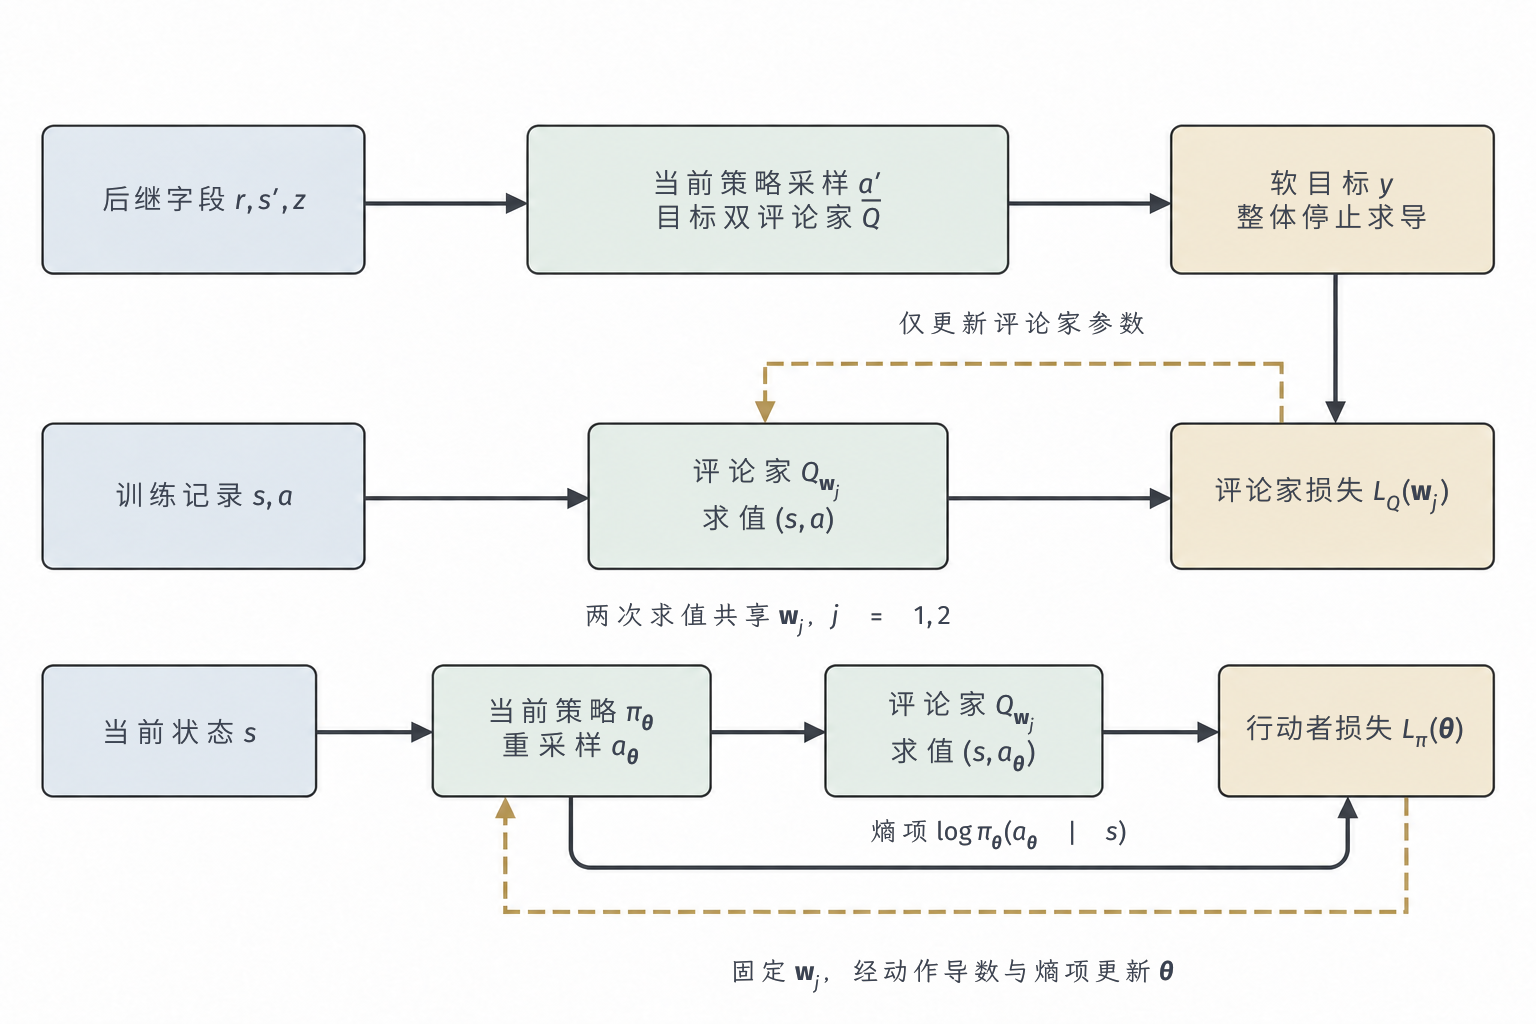
\includegraphics[width=157.400mm]{figures/10-reinforcement-learning/01-problems-and-solving/generated/rl-learning-sac/figure.png}
  \caption{SAC的目标构造、评论家拟合与行动者改进。上排由后继训练字段构造停止求导的软目标；中排用回放记录动作求值并拟合目标；下排在当前状态重新采样策略动作，再调用共享参数的评论家优化行动者。行动者更新固定评论家参数，保留其对动作的导数；目标中的后继动作来自当前策略，软价值由目标评论家计算，整个目标停止求导。}
  \label{fig:rl-learning-sac}
\end{figure*}

温度可以由目标熵$H_0$自动调整。令$\alpha=e^\xi$，对
$L_\alpha(\xi)=
\widehat{\mathbb E}[e^\xi(-\log\pi_{\bm\theta}(a\mid s)-H_0)]$
下降，且在此步固定策略样本和对数密度。当前熵低于目标时梯度为负，$\xi$上升，从而提高探索的熵奖励；高于目标时方向相反。连续动作的$H_0$可以为负，不应把它当成离散动作数的对数。算法\ref{alg:rl-learning-sac}明确了更新顺序；独立价值网络被移除与自动温度来自后续SAC算法版本，应与最初论文的实现区分\scite{rl3-haarnoja2018applications}

\begin{algorithm}[SAC的真实数据与离策略更新循环]
  \label{alg:rl-learning-sac}
  \begin{algorithmic}[1]
    \State 初始化策略、两个评论家、对应目标评论家、温度及真实回放$D$。
    \For{每个真实交互步}
      \State 由当前策略采样动作并执行，记录$(s,a,r,s',z)$；预热阶段可使用指定随机策略。
      \State 将经验写入$D$；真实终止或环境时间上限要求重置时取得新起点，否则转到$s'$。
      \State 仅时间截断仍令$z=0$，记录中的$s'$保留重置前的后继观测。
      \For{预先规定的$U$次梯度更新}
        \State 从$D$抽批次，在后继状态按当前策略采样$a'$，构造停止求导的$y$。
        \State 两个评论家分别最小化$L_Q$，不向目标网络和目标动作反向传播。
        \State 在同批状态重新采样可重参数化动作，固定评论家参数，最小化$L_\pi$。
        \State 若自动调温，固定策略输出并最小化$L_\alpha$。
        \State 目标参数更新为$\bar{\bm w}_j\gets(1-\tau)\bar{\bm w}_j+\tau\bm w_j$。
      \EndFor
    \EndFor
  \end{algorithmic}
\end{algorithm}

例如一条人工经验有$r=0.1$、$\gamma=0.9$、$z=0$，
后继动作的两个目标值为$(0.7,0.9)$，
$\log\pi(a'\mid s')=-0.5$、$\alpha=0.2$，则$y=0.1+0.9(0.7+0.1)=0.82$。
若一个表格评论家当前值为$0.6$，步长$0.1$的一次平方损失更新得到$0.622$。
在当前状态另采一个动作，若$\min Q=0.65$、$\log\pi=-0.8$，其行动者损失样本为$-0.16-0.65=-0.81$；这个数值还不足以决定参数步长，必须通过密度和$Q$的动作导数求梯度。它不等于用记录动作做监督学习。

离策略和近端约束也可以按其他方式组合。表\ref{tab:rl-learning-off-policy-actors}比较四种接口，关注的是概率比在哪个位置校正旧策略轨迹的抽样分布、哪些参数被当作旧策略，而非把分布式采样本身当成学习保证。

这些组合分别针对不同的复用困难。ACER（actor--critic with experience replay）保留截断重要性比之外的补偿，使少抽样动作的贡献不被直接丢掉。IMPALA将采样器与学习器分开，V-trace用来处理两边策略版本的差异。MPO（maximum a posteriori policy optimisation）先在评论家评分下求一份改进的动作分布，再用参数策略拟合这份分布；这里两步的目标和约束不同。APPO（asynchronous proximal policy optimization）则在异步采集的轨迹记录上组合离策略目标与近端代理。下面的表是这些职责的汇总，具体保证仍由校正位置和抽样条件决定。

\begin{table*}[t]
  \centering
  \small
  \begin{tabularx}{\linewidth}{>{\raggedright\arraybackslash}p{17mm} >{\raggedright\arraybackslash}X >{\raggedright\arraybackslash}X}
    \toprule
    方法 & 校正或约束的位置 & 轨迹采样接口与边界 \\
    \midrule
    ACER & 截断重要性比率加偏差校正项，配合Retrace评价及策略变化约束 & 回放与当前采样结合；只截断而丢掉补偿项不是相同估计器 \\
    IMPALA & V-trace校正行为策略与学习器策略差异 & 解耦采样和学习；截断阈值影响评价目标，见前文V-trace \\
    MPO & E步构造受KL约束的动作改进分布，M步在约束下拟合参数策略 & 常用回放状态和评论家；动作改进与状态分布覆盖是不同问题 \\
    APPO & 异步采样下结合V-trace目标与近端概率比代理 & 行为、目标和学习策略可能不同；须报告具体实现的目标同步及比率定义 \\
    \bottomrule
  \end{tabularx}
  \caption{轨迹记录复用、策略滞后和更新约束的几种组合。APPO是实现族名称，不能假定所有版本具有同一估计目标。}
  \label{tab:rl-learning-off-policy-actors}
\end{table*}

\Needspace{24\baselineskip}
ACER的重要性截断补偿需要同时保留被截断部分的期望校正；否则得到的是另一个有偏梯度\scite{rl3-wang2017acer}
Retrace提供评价目标，策略变化约束则限制更新幅度，两者不能替代概率比支持条件。

MPO的受约束动作分布改进与参数拟合分成两步，能分别控制非参数改进和参数投影。回放状态仍来自行为分布，动作分布上的KL约束并不自动解决未覆盖状态的问题\scite{rl3-abdolmaleki2018mpo}

\Needspace{18\baselineskip}
IMPALA已经在离策略评价中出现。APPO的具体工程版本应以使用的实现文档为准\scite{rl3-rllib-appo}
训练报告需要保存版本与配置，不能只写一个缩写就省去旧策略的定义。

% Outline: 3.3.6
\subsection{正则化与无梯度策略搜索}
\label{sec:rl-learning-regularized-search}

熵奖励鼓励保留多个动作，KL约束则限制离开参考行为。固定某状态的动作评分后，可以把两者写成同一个局部选择问题：在合法动作的概率分布中，增大平均评分，同时惩罚相对参考分布的KL。给定$q_a$、$p_a^{\mathrm{ref}}$和$\alpha>0$，考虑
\[
  \max_p\left\{\sum_a p_a q_a
          -\alpha D_{\mathrm{KL}}(p\Vert p^{\mathrm{ref}})\right\}.
\]
在参考分布的正支撑上，对概率归一化约束引入乘子并求导，
$q_a-\alpha(\log(p_a/p_a^{\mathrm{ref}})+1)-\lambda=0$，
从而
\begin{equation}
  p_a^{\mathrm{new}}
     =\frac{p_a^{\mathrm{ref}}e^{q_a/\alpha}}
            {\sum_b p_b^{\mathrm{ref}}e^{q_b/\alpha}}.
  \label{eq:rl-learning-exponential-update}
\end{equation}
参考分布取均匀分布时回到熵正则；取旧策略时得到KL几何下的一步镜像上升。若评分取当前精确优势、$\alpha=(1-\gamma)/\eta$，就得到式\eqref{eq:rl-learning-tabular-npg-step}的表格NPG策略更新；相应全局进展还依赖定理中的精确评价、初始化与共同目标条件。若$p_a^{\mathrm{ref}}=0$，任何给该动作正质量的$p$都会产生无限KL，更新无法重新发现它。这是支持集的限制，不是温度再小就能克服的数值问题。

式\eqref{eq:rl-learning-exponential-update}也说明参考分布的作用。仍取评分$(0.7,0.4)$、$\alpha=0.3$，若旧动作概率为$(0.2,0.8)$，新概率按$(0.2e,0.8)$归一化，高评分动作只增至约$0.4046$；若参考概率均为$1/2$，它会增至约$0.7311$。相同评分在不同参考分布下形成不同更新，因为这里既奖励高评分，也惩罚离开旧行为。这种在分布几何中作局部上升的做法称为镜像上升（mirror ascent）。

图\ref{fig:rl-learning-regularized-search}上半部展示这一局部更新。相似的指数权重也可从概率条件化得到，这一视角称为\term{控制即推断}（control as inference）：把奖励较高的轨迹赋予较大的“最优性”事件概率，再推断条件于该事件的行为。在离散有限时域模型中，设最优性变量的条件概率与$\exp(r_t/\alpha)$成比例，给定动作先验和真实动力学，轨迹后验便按指数回报重加权。不过，随机环境的精确后验还可能偏好幸运转移，而策略无法控制这种运气。要对应可执行控制，需固定变分轨迹族的真实环境核，只优化策略，并说明近似推断范围。因此这个构造可以解释某些熵与KL目标，不能把所有策略算法都视为同一精确后验求解\scite{rl3-levine2018inference}

以上更新需要动作评分或梯度。若策略包含不可微程序，或者只能在整回合结束后查询回报，可以改为试验多组策略参数。\term{交叉熵方法}（cross-entropy method, CEM）维护参数搜索分布，保留估计回报较高的一部分候选作为精英，再拟合这些候选以改变下一轮试验范围。若搜索分布为高斯，第$k$轮采样
$\bm\theta_i\sim\mathcal N(\bm m^{(k)},\bm C^{(k)})$，按估计回报选出精英集合$\mathcal E$，则未平滑更新为
\[
  \bm m^{(k+1)}
       =\frac1{|\mathcal E|}\sum_{i\in\mathcal E}\bm\theta_i,
  \qquad
  \bm C^{(k+1)}
       =\frac1{|\mathcal E|}\sum_{i\in\mathcal E}
       (\bm\theta_i-\bm m^{(k+1)})
       (\bm\theta_i-\bm m^{(k+1)})^\top.
\]
实际可设置最小协方差或平滑更新，防止过早塌缩。图\ref{fig:rl-learning-regularized-search}下半部使用独立一维教学回报
$F(\theta)=-(\theta-1)^2$：四个候选为$(-1,0,1,2)$，得分$(-4,-1,0,-1)$；预先约定并列时选较小参数，保留两名精英$(0,1)$，得到新均值$0.5$、最大似然方差$0.25$。这里的候选与得分都是人工给定，不是一次真实训练的测量结果\scite{rl3-rubinstein1999crossentropy}

\begin{figure*}[t]
  \centering
  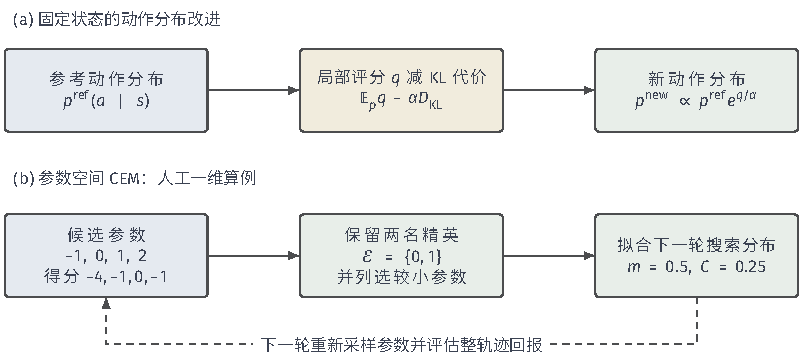
\includegraphics[width=135.961mm]{figures/10-reinforcement-learning/01-problems-and-solving/tikz/rl-learning-regularized-search.pdf}
  \caption{两类策略搜索分布。上排在固定状态对动作分布做正则化改进，下排在参数空间选择精英并拟合搜索分布；动作概率与参数采样概率不能混为一谈。}
  \label{fig:rl-learning-regularized-search}
\end{figure*}

交叉熵方法的名称来自拟合搜索分布：把精英候选看成经验目标分布，提高搜索分布在这些候选上的平均对数密度，等价于减少相应交叉熵。高斯情况下得到精英均值与协方差。这里被拟合的是“下一轮试哪些参数”的分布，不是状态下的动作策略；最终仍需从候选或搜索结果中确定一份可执行策略。

CEM只用精英筛选和拟合改变搜索分布，进化策略（evolution strategies, ES）还可以用参数扰动与回报的关系估计方向。先将原目标在高斯邻域内平均，定义
$F_\sigma(\bm\theta)=
\mathbb E_{\bm\epsilon\sim\mathcal N(\bm0,\bm I)}
J(\bm\theta+\sigma\bm\epsilon)$，则在可积条件下
\[
  \nabla F_\sigma(\bm\theta)
    =\frac1{\sigma}\mathbb E[J(\bm\theta+\sigma\bm\epsilon)\bm\epsilon].
\]
使用成对扰动可估计为
$(2N\sigma)^{-1}\sum_i
[\,\widehat J(\bm\theta+\sigma\bm\epsilon_i)
-\widehat J(\bm\theta-\sigma\bm\epsilon_i)\,]\bm\epsilon_i$。
\Needspace{16\baselineskip}
它求的是平滑后的参数目标，$\sigma$既决定探索范围也改变平滑偏差\scite{rl3-salimans2017es}

\Needspace{16\baselineskip}
CMA-ES进一步用选择结果及跨轮演化路径更新协方差和全局步长，使参数试验适应不同方向的尺度；并非仅把CEM的样本协方差换个名字\scite{rl3-hansen2001cma}

参数空间探索让一整段行为保持同一次参数扰动，可能形成时间一致的探索；每步动作噪声则在同一策略附近不断改变局部控制。前者不能免费绕过长时程困难：每组参数仍需足够回合才能辨认真实回报，高维全协方差要存储和估计二次数量的参数，排名还会被回报噪声改变。是否值得使用，应比较总真实交互、可并行程度、策略可微性和搜索维度，而不是只比较一次更新公式的长度。

% Outline: 3.4
\section{基于模型的价值学习}
\label{sec:rl-learning-model-value}

回放可以重复使用记录，却不能直接回答某个未记录动作的后果。学习环境模型把已见经验拟合成可查询的后继和奖励预测器，用它补充价值更新或当前动作比较。模型预测有两种直接用途：Dyna生成模拟经验后更新动作价值；MPC预测当前候选轨迹的回报，选出计划后只执行首动作。MPC未必训练独立价值函数，但动作仍由预计回报比较产生。用模型训练跨状态共享的参数策略，则能把部分搜索计算转移到训练阶段，供执行时直接调用。

% Outline: 3.4.1
\subsection{环境模型的表示与不确定性}
\label{sec:rl-learning-model-representation}

在基准网格的$(3,2)$执行向右，后继位置可能为$(4,2)$、$(3,3)$或$(3,1)$，概率分别是$0.8,0.1,0.1$。若把坐标当连续量并最小化平方预测误差，最优输出是条件均值$(3.8,2)$，但网格没有这个状态。平均位置既不能告诉规划器滑移会通往哪里，也不能直接代入只在合法格点上定义的价值函数。预测损失选错对象，甚至会使一个统计上正确的条件均值不适合控制。

对这个网格，合适的模型应给每个合法落点分配概率。假设在同一状态动作下观察到10次结果，其中8次到$(4,2)$、另外两个落点各1次，经验概率就是$(0.8,0.1,0.1)$。这些是教学计数，恰好与真实概率一致；实际有限样本未必如此。给定$(s,a)$后输出一份后继概率分布，就是转移概率核在这里的含义；“核”强调每个输入各有一份分布，不要求它是某个核函数。

拟合概率也需要选择准则。将每条记录的已发生后继代入预测分布，所有记录的概率相乘形成似然；取负对数后乘积变成可累加的损失。上述计数下，候选概率$(p_1,p_2,p_3)$的平均损失为$-[8\log p_1+\log p_2+\log p_3]/10$。在概率非负且和为1的约束下，最小化它得到相应经验频率。后面的神经模型保留这一“给实际结果较高概率”的原则，只是不同状态动作会共享参数。

\begin{definition}[学得环境模型的预测对象]
  \label{def:rl-learning-learned-model}
  设$S$与$\mathsf A$为可测空间，合法状态动作域为$X=\{(s,a):s\in S,\ a\in\mathsf A(s)\}$，并在$X$上约定可测结构。\term{确定性动力学模型}的候选是可测映射$\widehat f_{\bm\phi}:X\to S$；\term{随机动力学模型}的候选是从$X$到$S$的概率核$\widehat T_{\bm\phi}(\cdot\mid s,a)$。给定训练记录和学习规则后得到的具体映射或核，称为学得的动力学模型。贝叶斯方法在参数或函数上保持给定先验与似然产生的后验，并对该后验积分得到预测；集成方法保留若干分别拟合的预测器，例如通过重采样训练记录和随机初始化得到。两者描述参数不确定性的处理方式，不与确定性或随机后继预测互斥。

  奖励均值模型为可测函数$\widehat R:X\to\mathbb R$，继续概率模型为可测函数$\widehat c(s,a,s')\in[0,1]$。也可学习$(s',r,c)$的联合概率核，以保留奖励、后继与继续事件之间的相关性。
\end{definition}
这些预测量需要从真实记录中学习，而不是按控制回报直接拟合。令$c_t=0$表示执行$a_t$后真正终止，$c_t=1$表示继续。对具备随机后继、条件奖励和继续预测的模型，可以最小化记录中三个结果的负对数似然；期望按真实回放记录的经验抽样律$\widehat P_{D_{\mathrm{real}}}$取，候选变量是模型参数$\bm\phi$：有限状态时，转移核可用条件质量函数表示；连续状态时，须先选定参考测度$\nu$，并限定候选核满足$\widehat T_{\bm\phi}(\cdot\mid s,a)\ll\nu$，用条件密度$\widehat t_{\bm\phi}=\mathrm d\widehat T_{\bm\phi}/\mathrm d\nu$计算似然。奖励项同样采用所选奖励参考测度下的质量或密度，继续标记采用伯努利质量。下面统一用$\widehat t_{\bm\phi}$表示相应的质量或密度；预测核仍记为$\widehat T_{\bm\phi}$。
\[
  \mathbb E_{\widehat P_{D_{\mathrm{real}}}}\!\left[
    \begin{aligned}
      &-\log\widehat t_{\bm\phi}(s_{t+1}\mid s_t,a_t)\\
      &-\log p_{\bm\phi}(r_t\mid s_t,a_t,s_{t+1})\\
      &-\log p_{\bm\phi}(c_t\mid s_t,a_t,s_{t+1})
    \end{aligned}
  \right].
\]
训练时，将每条真实记录中的后继状态、奖励和继续标记分别送入三项负对数似然，更新模型参数。使用时，规划器给定$(s,a)$，先抽取预测后继，再生成相应奖励和继续标记；若预测可以继续，就从该后继展开下一步，否则结束这条模拟轨迹。这样得到的轨迹可用于计算候选动作的预计回报。上述损失评价的是模型对记录的预测，策略目标则评价依这些预测选择动作后能取得多少回报。

生成联合样本时，还需明确三个预测之间的依赖。将上面三项对应的分布直接相乘，隐含了给定$(s,a,s')$后奖励与继续标记条件独立的假设；若不成立，应直接拟合它们的联合分布，或让继续预测再以奖励为条件。只计算期望回报的Bellman备份时，即时奖励的条件均值已经足够；要模拟风险或奖励与后继状态的联合事件，则需保留相应的分布与相关性。终止标签也必须来自任务本身：因采集上限中断的记录不能直接标成$c_t=0$，否则模型会把记录结束学成任务结束。

确定性模型则给每个输入只输出一个后继。它适合确实确定的系统，或明确采用确定性近似的计算；若真实转移随机，输出一个均值不能自动代替随机模型。模型集成又处在另一层：每个成员本身都可以输出一份随机后继分布，成员间差异表示拟合解释的分歧，成员内随机性表示该解释允许的多种后果。这延续了前面认知与偶然不确定性的区分，但成员分歧仍需校准才能成为置信量。

当观测是图像时，可先编码成潜在状态，再预测潜在后继。图\ref{fig:rl-learning-model-anatomy}和表\ref{tab:rl-learning-model-representations}拆开了这些部件。潜在模型沿用上述训练和使用过程，只是把显式状态换成内部表示，并可增加图像重建目标来训练编码器。

潜在状态（latent state）是编码器从观测或历史计算的内部变量，目的是用较小表示支持后续预测。它的坐标不必是可直接测量的位置或速度；例如网络可以把一幅图像压成一个向量，再让动力学预测下一向量。潜在预测减少了每一步还原像素的成本，但“向量维数小”本身不保证它保留门的位置、机器人的速度或其他会改变动作后果的状态分量。

这一替换要求表示保留预测动作后果和比较长期回报所需的观测历史差别。当前一帧看不出速度时，需要结合历史构造表示；单帧重建再准确也不能补回速度。RSSM一类递归状态空间模型如何从历史形成状态，将在第\ref{chap:rl-information}章处理。模型使用给定表示进行预测的机制，与观测历史能否形成充分决策依据，需要分别分析。

\begin{figure*}[t]
  \centering
  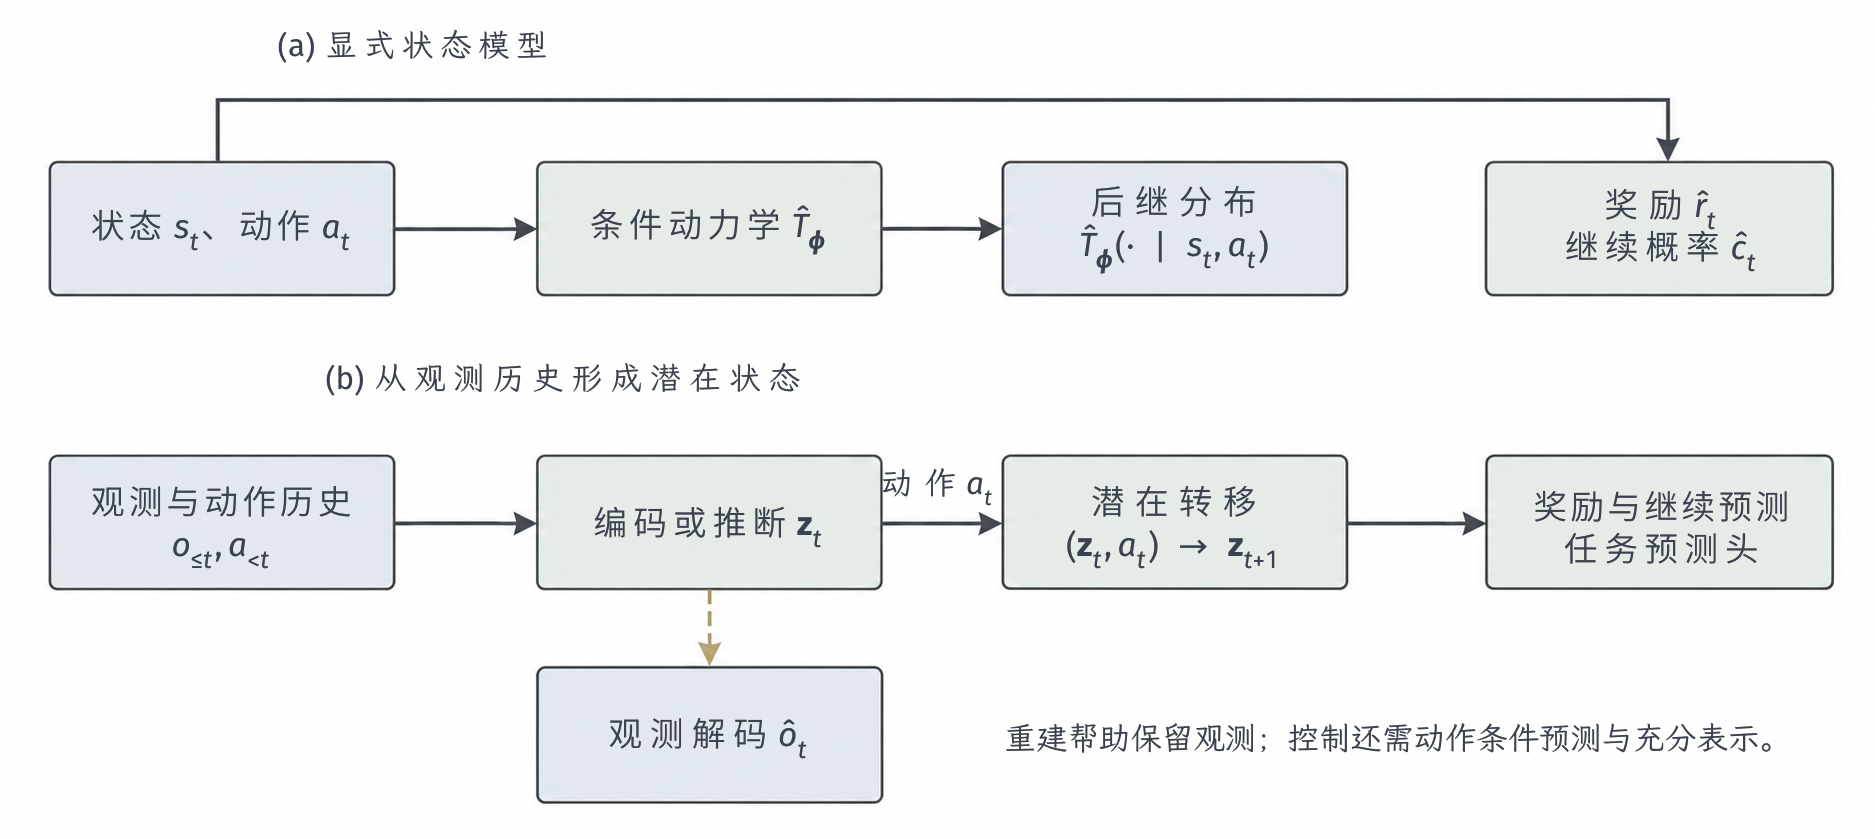
\includegraphics[width=157.400mm]{figures/10-reinforcement-learning/01-problems-and-solving/generated/rl-learning-model-anatomy/figure.png}
  \caption{学习模型的预测职责。上排直接预测可观测状态，下排先形成潜在状态；解码重建、奖励与继续预测是不同预测任务，是否需要每项预测取决于下游用途。虚线表示可选的重建支路，不表示模型生成经验。}
  \label{fig:rl-learning-model-anatomy}
\end{figure*}

\begin{table*}[t]
  \centering
  \small
  \begin{tabularx}{\linewidth}{>{\raggedright\arraybackslash}p{25mm} >{\raggedright\arraybackslash}X >{\raggedright\arraybackslash}X}
    \toprule
    表示与实例 & 拟合和保留什么 & 控制接口与局限 \\
    \midrule
    显式状态模型 & 对位置、速度等已定义状态拟合后继分布；奖励可已知或另学 & 可直接将后继送入价值函数；坐标误差须结合状态尺度与决策后果解释 \\
    World Models & 用VAE压缩图像，以混合密度递归模型预测潜在演化，控制器读取表示与记忆 & 控制器可用进化搜索训练；不同任务中模型承担表示或模拟器职责，不等于每步都做MPC \\
    PlaNet & 确定递归分量与随机潜变量共同形成RSSM；拟合观测、奖励及潜在多步关系 & 在潜在空间评估动作序列并执行首动作；搜索质量仍依赖模型滚动和状态推断 \\
    \bottomrule
  \end{tabularx}
  \caption{显式与潜在模型的区别。随机潜变量、参数后验和模型集成是不同层面的不确定性表示。}
  \label{tab:rl-learning-model-representations}
\end{table*}

\Needspace{18\baselineskip}
World Models展示了压缩视觉、递归预测与小型控制器的组合\scite{rl3-ha2018worldmodels}
PlaNet进一步将潜在模型直接用于在线规划，二者所需的训练目标与执行成本并不相同\scite{rl3-hafner2019planet}

评价模型时至少要分清三件事。一步测试误差检查测试转移样本所代表的状态动作分布上的局部预测；多步闭环误差检查策略根据预测状态继续行动后的偏离；不确定性校准检查标成某个置信水平的集合是否具有相应覆盖率。一个只在远离门口处略有坐标误差的模型，可能控制得很好；另一个平均误差更小的模型，若恰好把门前可通行格预测成墙另一侧，就会改变最优动作。在连续化房间示例中，两条预测只相差很小距离也可能落在碰撞边界两侧，后果不能按平均像素距离比较。

集成分歧可以定位模型之间尚未达成一致的区域，但所有成员若共享训练缺口、特征缺陷或错误归纳偏置，也可能一致地错。只有另有统计假设和校准过程时，集成方差才能解释为某种置信半径；不能把“多个网络很一致”直接换成“真实环境一定如此”。

% Outline: 3.4.2
\subsection{模型生成经验与价值更新}
\label{sec:rl-learning-dyna}

观察到通往终点的转移后，上游状态可能很久不再被访问，已取得的奖励样本却可以先通过已有模型影响上游估值。Dyna把真实经验更新和模型内规划接到同一Q-learning接口：先从真实样本学习，再抽取模型后果重复备份。对样本$(s,a,r,s',c)$，无论其来源如何，更新均为
\begin{equation}
  Q(s,a)\gets Q(s,a)+\alpha
  \left[r+\gamma c\max_bQ(s',b)-Q(s,a)\right].
  \label{eq:rl-learning-dyna-update}
\end{equation}
差别在于这条样本可能来自真实环境，也可能来自模型。图\ref{fig:rl-learning-dyna}用线型标出两类来源，算法\ref{alg:rl-learning-dyna}给出一个支持随机转移的表格版本。原始确定性Dyna-Q可以只记每个状态动作最后观察到的后果；随机网格应保存经验分布或学习一个能采样多种后果的模型\scite{rl3-sutton1991dyna}

\begin{figure*}[t]
  \centering
  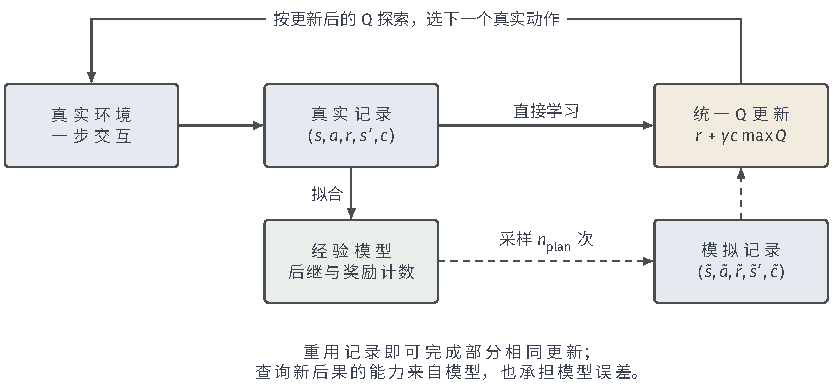
\includegraphics[width=140.959mm]{figures/10-reinforcement-learning/01-problems-and-solving/tikz/rl-learning-dyna.pdf}
  \caption{Dyna的转移记录生成与价值更新路径。实线为真实交互及其记录，虚线为学习模型生成的经验；两者进入同一种Q更新。模型采样次数是规划计算量，不是新增真实交互量。}
  \label{fig:rl-learning-dyna}
\end{figure*}

\begin{algorithm}[随机表格Dyna的一轮交互]
  \label{alg:rl-learning-dyna}
  \begin{algorithmic}[1]
    \State 在$s_t$按$Q$的探索策略选择$a_t$，真实执行并记录$(r_t,s_{t+1},c_t)$。
    \State 用式\eqref{eq:rl-learning-dyna-update}更新真实访问的$Q(s_t,a_t)$。
    \State 更新该状态动作的后继、奖励及继续标记计数，形成经验联合模型。
    \For{$i=1,\ldots,n_{\mathrm{plan}}$}
      \State 从已见状态动作中按指定规划分布选择$(\widetilde s,\widetilde a)$。
      \State 从当前经验模型采样$(\widetilde r,\widetilde s',\widetilde c)$。
      \State 用同一Q更新式更新$Q(\widetilde s,\widetilde a)$。
    \EndFor
    \State 若真正终止或达到环境的重置上限则重置；否则从$s_{t+1}$继续。仅时间截断时记录仍保留$c_t=1$及重置前的后继。
  \end{algorithmic}
\end{algorithm}

\begin{example}[不返回上游也能传播一次奖励]
  \label{ex:rl-learning-dyna-grid}
  在基准网格中，假设此前记录过
  $((3,2),\text{右},-0.04,(4,2),1)$，但当时所有Q值为0。
  现在从$(4,2)$向上恰好进入终点，用步长1把$Q((4,2),\text{上})$更新为1。
  若本轮模型从第一条记录生成相同转移，上游目标便为
  $-0.04+0.9\times1=0.86$。从当前上游Q值0出发、取规划步长$0.5$，一次模拟更新得到$0.43$，无需真实返回$(3,2)$。

  这是单条经验模型的一次更新，不是随机网格的精确Bellman备份。
  若其他后继的最大Q值仍为0，使用真实转移核的该次备份目标应为
  $-0.04+0.9(0.8\times1)=0.68$。模型中暂未记录的滑移不能因为多做模拟而消失。
\end{example}

对这条已经记录的转移，经验回放也能得到同样的$0.43$。模型的额外能力不在于重复这条算术，而在于按概率组合后果、查询未记录但可泛化到的动作，或递归生成新状态。表\ref{tab:rl-learning-generated-experience}因此把已有转移记录的复用与模型泛化分开。优先扫描还可按价值变化沿模型中的前驱关系分配规划次数；这种计算调度可以加快价值变化沿模型前驱关系的传播，但不能增加对未观察状态动作后果的真实验证。

\begin{table}[htbp]
  \centering
  \small
  \begin{tabularx}{\linewidth}{>{\raggedright\arraybackslash}p{21mm} >{\raggedright\arraybackslash}X >{\raggedright\arraybackslash}X}
    \toprule
    经验来源 & 可重用或生成什么 & 额外风险 \\
    \midrule
    经验回放 & 原始记录中的完整转移 & 覆盖不足、旧策略分布与相关性 \\
    经验表格模型 & 已见状态动作的估计后果，可求期望或采样 & 有限计数误差，重复模型采样不增加真实转移记录 \\
    参数化模型 & 在新的状态动作处预测，并递归滚动 & 分布外泛化、终止错误及虚构可达状态 \\
    \bottomrule
  \end{tabularx}
  \caption{真实记录与生成经验。更灵活的查询接口同时引入了更强的模型正确性要求。}
  \label{tab:rl-learning-generated-experience}
\end{table}

这也解释了优先扫描（prioritized sweeping）的调度对象。若某状态的价值刚大幅改变，模型中能一步到达它的状态动作称为它的前驱；优先备份这些前驱，再把新的变化向更早位置传播，就能把计算用在受影响的区域。这里的优先级控制模型备份顺序，与优先回放按记录残差改变抽样概率相关但不同；两者都不能替代一次新的真实试验。

Dyna增加多次分别采样的一步备份；也可以把连续几步预测合成当前状态的一次目标。这称为\term{模型价值扩展}（model-based value expansion, MVE）：短段奖励由模型预测，余下未来交给末端评论家。从真实回放状态$\widetilde s_0=s$出发，按待评价策略和学习模型滚动$L$步；令$\widetilde c_j$为继续标记，$w_0=1$、$w_{j+1}=w_j\widetilde c_j$，用累积继续权重屏蔽终止后的贡献，得到
\begin{equation}
  \widehat G^{\mathrm{MVE}}_0
  =\sum_{j=0}^{L-1}\gamma^j w_j\widetilde r_j
    +\gamma^L w_L V_{\bar{\bm w}}(\widetilde s_L).
  \label{eq:rl-learning-mve}
\end{equation}
奖励、后继和继续标记来自模型，起点来自真实回放中的状态记录，末端价值来自目标评论家。若预测的是联合期望，应对联合滚动取期望；不能在存在相关性时任意用各自边缘均值的乘积替代。以动作价值为目标时，第一步固定待更新动作，后续才由评价策略选动作。评论家把$\widehat G^{\mathrm{MVE}}_0$视为停止求导的目标，不在这一步沿模型反向优化策略\scite{rl3-feinberg2018mve}

若模型完全正确且没有终止，末端评论家的统一误差$\epsilon_V$只贡献$\gamma^L\epsilon_V$。增大$L$会衰减这项，却增加了需要正确预测的奖励和状态数。例如一个独立教学滚动有$L=2$、预测奖励$(0.1,0.2)$、末端价值$0.5$，则目标为$0.1+0.9(0.2)+0.9^2(0.5)=0.685$；若第二步错误预测为终止，就丢失$0.405$的末端贡献。滚动更长不是单向改善，也不能把生成一百万条轨迹解释为获得了一百万条独立真实证据。

% Outline: 3.4.3
\subsection{学习模型上的预测控制}
\label{sec:rl-learning-learned-mpc}

在当前状态，模型也可以直接比较候选计划，不必先将结果写进长期Q表。第\ref{sec:rl-planning-horizon-search}节的闭环仍然适用：优化计划，只执行首动作，再用新观测重新规划。新增条件是动力学由已采集的真实转移记录拟合；为控制计算量，每轮优化还限制为预先给定的开环动作序列。若不同随机后继需要不同后续动作，一条固定序列不能表示这种反馈选择，即使模型准确也有限制。因此，前章针对反馈决策树的前瞻保证不能直接移用。图\ref{fig:rl-learning-mpc}标明真实纠正发生在哪里：环境只反馈已执行动作，不会验证本轮所有候选轨迹。

\begin{figure*}[t]
  \centering
  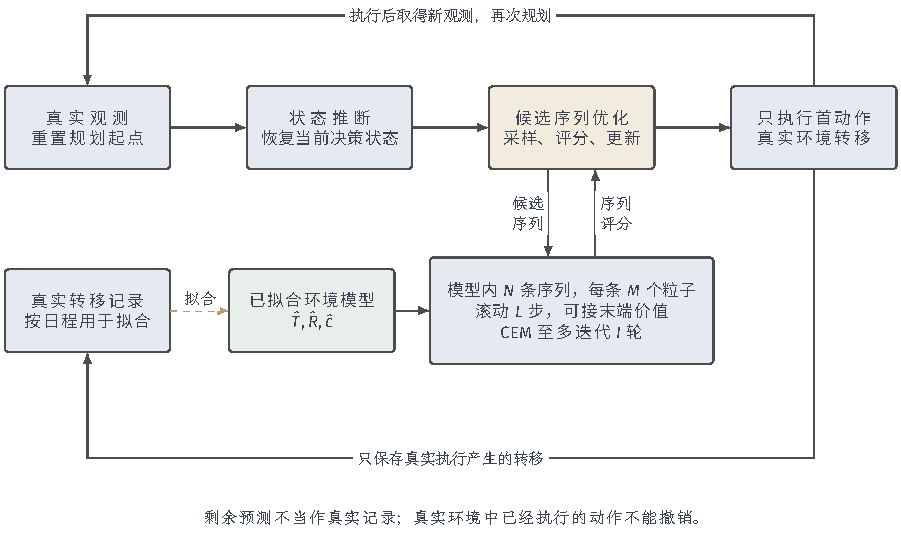
\includegraphics[width=152.615mm]{figures/10-reinforcement-learning/01-problems-and-solving/tikz/rl-learning-mpc.pdf}
  \caption{学习模型上的滚动规划。候选动作序列进入模型滚动，序列评分返回优化器；真实交互记录用于拟合环境模型。每轮从新观测建立规划起点，优化后只执行首动作；模型拟合可以较低频率进行，预测轨迹不会当作真实记录写回。}
  \label{fig:rl-learning-mpc}
\end{figure*}

当前规划的变量是一份动作序列，不是一份供所有状态调用的策略。在随机模型中，同一序列可能产生多条后继路径；粒子轨迹就是反复采样这些可能路径，用平均回报估计该序列的期望结果。候选数控制比较多少种计划，粒子数控制每种计划的评分波动，时域控制看多远。三者争用模型查询预算，增加一种数量不等于同时改善另外两种。

以有界连续动作$\bm u_j\in[\bm u_{\min},\bm u_{\max}]$为例，候选集合是长度$L$的合法动作序列。每条序列在模型中生成$M$个随机粒子轨迹，用平均预测奖励加末端价值估计期望回报，再选择评分较高的序列。评分为
\begin{equation}
  \widehat F(\bm u_{0:L-1};s)
  =\frac1M\sum_{m=1}^{M}
  \left[\sum_{j=0}^{L-1}\gamma^j\widehat r_j^{(m)}
          +\gamma^L\widehat V(\widehat s_L^{(m)})\right].
  \label{eq:rl-learning-particle-mpc}
\end{equation}
每个粒子从同一当前状态或其推断分布出发，经模型采样传播；终止时停止奖励并去掉末端价值。PETS（probabilistic ensembles with trajectory sampling，带轨迹采样的概率模型集成）使用概率动力学集成和轨迹粒子传播：模型内输出的噪声刻画随机后继，不同集成成员的预测差异反映模型拟合的不一致。其TS1传播可在每一步重选模型成员，TS$\infty$则让一个粒子在整个候选轨迹上保持同一成员；后者保留了“同一套动力学解释”在时间上的相关性，二者并不是同一个联合预测分布\scite{rl3-chua2018pets}

表\ref{tab:rl-learning-trajectory-optimizers}比较三种轨迹优化器。CEM在这里搜索的是本轮动作序列，不是前文跨状态共享的策略参数。一个可复现的教学配置为$L=5$、每轮$N=200$条候选、每条$M=20$个粒子、保留$E=20$条精英、最多$I=5$轮。初始化独立各维高斯，均值取上一步最优序列左移后的热启动，最后一步补零，标准差取动作范围的一半；第一轮没有历史序列时全取零均值。

\begin{table*}[t]
  \centering
  \small
  \begin{tabularx}{\linewidth}{>{\raggedright\arraybackslash}p{18mm} >{\raggedright\arraybackslash}X >{\raggedright\arraybackslash}X}
    \toprule
    优化器 & 候选和更新机制 & 奖励查询、梯度需求与预算 \\
    \midrule
    随机shooting & 从固定提议分布抽序列，选择预计回报最高者 & 无梯度；一次评估$N$条，不利用精英改变下一轮分布 \\
    CEM & 反复采样，截取精英，对序列分布重新做最大似然拟合 & 无梯度；需报告轮数、精英比例、方差下限及约束处理 \\
    MPPI & 对名义序列加入噪声，用指数回报或负成本权重平均扰动 & 标准路径积分推导有动力学与噪声匹配条件；通用采样实现需说明重要性校正与控制代价 \\
    \bottomrule
  \end{tabularx}
  \caption{同一模型目标的不同优化接口。PETS和PlaNet是模型与规划器的组合，不能与CEM这样的优化器放在互斥层级。}
  \label{tab:rl-learning-trajectory-optimizers}
\end{table*}

每轮从当前高斯采样并逐坐标裁剪到动作区间，按式\eqref{eq:rl-learning-particle-mpc}评分，取最高$E$条；并列按候选编号决定。用精英的逐坐标均值$\bm m_{\mathcal E}$和方差$\bm v_{\mathcal E}$更新
\[
  \bm m\gets\tfrac12\bm m+\tfrac12\bm m_{\mathcal E},
  \qquad
  \bm v\gets\max\{\bm v_{\min},
                      \tfrac12\bm v+\tfrac12\bm v_{\mathcal E}\},
\]
其中每个坐标的最小标准差预设为动作范围的$1\%$。此处“裁剪高斯”是具体实现选择，不冒充截断高斯的精确最大似然算法。完成5轮即停止，保留所有已评分候选中分数最高的一条，执行其首动作；不把未经重新评分的均值序列自动当成最佳候选。这样每个真实动作最多需要$INML=100\,000$次粒子转移调用，另加$INM$次末端价值调用。批量并行会改变耗时，但不改变这个查询计数。上述数字只用于明确预算，不是PETS的统一默认值。

MPPI式加权把本轮候选序列的评分$\widehat F_i$转成归一化权重，常写为$w_i\propto\exp((\widehat F_i-\max_j\widehat F_j)/\tau)$，其中$\tau>0$是温度，所有$w_i$的和为1。温度越小，相同评分差产生的权重比越悬殊；减去最大值只为数值稳定，不改变归一化权重。再用$\sum_iw_i\bm\epsilon_i$修正名义序列，其中$\bm\epsilon_i$是生成第$i$条候选时加入的序列扰动。如果采样分布不等于推导中的参考分布，或控制噪声结构改变，就须补相应权重，不能从这个指数形式单独推出路径积分最优控制结论\scite{rl3-williams2017mppi}

PlaNet把候选动作送入潜在动力学，以预测奖励评估序列，使用CEM选择动作；它不需要为每个候选解码整段像素。PETS则通常在给定状态坐标上预测动力学。两者都能闭环重规划，但预测对象、状态推断和每次查询成本不同。

墙边滑移说明重规划的边界。在基准网格的$(4,2)$向上，真实到达终点的概率是$0.8$，还可能左滑至$(3,2)$或撞右墙原地不动。一个错误模型若把成功概率估为$0.98$，短时域会高估立即结束的机会；过短时域且无末端价值又可能低估绕行，长时域则继续使用错误转移。下一次观测能告诉规划器这次是否滑移，却不能在动作执行前补回遗漏的风险。若把墙改成不可逆损失区域，重规划也无法撤销落入其中的动作；这种约束需要第\ref{chap:rl-trustworthy}章的安全条件，而不是单靠“闭环”一词。

% Outline: 3.4.4
\subsection{面向搜索的模型与表示}
\label{sec:rl-learning-muzero}

搜索比较向左和向右，直接需要的是各分支的奖励及长期价值，而非每个背景像素。若潜在模型在所用展开深度上保留这些预测量，并提供值得优先检查的动作，规划器就可能据此选择。MuZero学习的正是服务于搜索的表示、动力学和预测头，不要求潜在状态还原完整观测；免去重建并没有免去决策相关预测的准确性要求\scite{rl3-schrittwieser2020muzero}

MuZero的三个部件可沿一次决策理解。表示函数把当前真实历史变成搜索起点；动力学接收一个候选动作，输出预测奖励与潜在后继；预测头在该后继给出叶值及动作先验。先验只帮助分配搜索次数，搜索返回值还要沿边加上奖励，最后用访问统计形成动作分布。网络在这里同时帮助预测和安排搜索，最终决策仍包含搜索计算。

为避免与决策时可得历史$I_t$混淆，记表示函数为$e_{\bm\phi}$。从实际记录的可得历史编码得到$\bm z^0=e_{\bm\phi}(I_t)$，潜在动力学与预测头为
\begin{equation}
  (\widehat r^k,\bm z^{k+1})=g_{\bm\phi}(\bm z^k,a^k),
  \qquad
  (\bm p^k,\widehat v^k)=f_{\bm\phi}(\bm z^k).
  \label{eq:rl-learning-muzero-model}
\end{equation}
$\bm p^k$是动作先验，不是最终搜索访问分布；$\widehat v^k$是叶值，不是从根开始的全部回报。沿搜索边备份时仍需加边上奖励：
$G^k=\widehat r^k+\gamma G^{k+1}$。
如果一条新边预测奖励$-0.04$、后继叶值$0.8$，其返回值就是$0.68$，不能把$0.8$原样抄回父节点。

搜索还需要分配有限展开次数，既检查当前返回值高的动作，也检查先验看好但尚少访问的动作。已展开节点存储访问数$N(\bm z,a)$和平均返回值$\overline Q(\bm z,a)$。在合法分支上最大化“返回值加探索项”，可用常数探索系数的PUCT形式说明：
\[
  a\in\argmax_b\left[
    \overline Q(\bm z,b)
    +c\,p(b\mid\bm z)
      \frac{\sqrt{\sum_{b'}N(\bm z,b')}}{1+N(\bm z,b)}
  \right].
\]
实际MuZero还使用随访问数变化的系数、价值范围归一化和训练时根噪声等细节；应按任务实现保存配置。这一评分沿树选择到叶节点，调用一次潜在动力学生成新节点，查询预测头，再沿路径增加计数并更新均值。图\ref{fig:rl-learning-muzero}分开了搜索备份与训练监督。

\begin{figure*}[t]
  \centering
  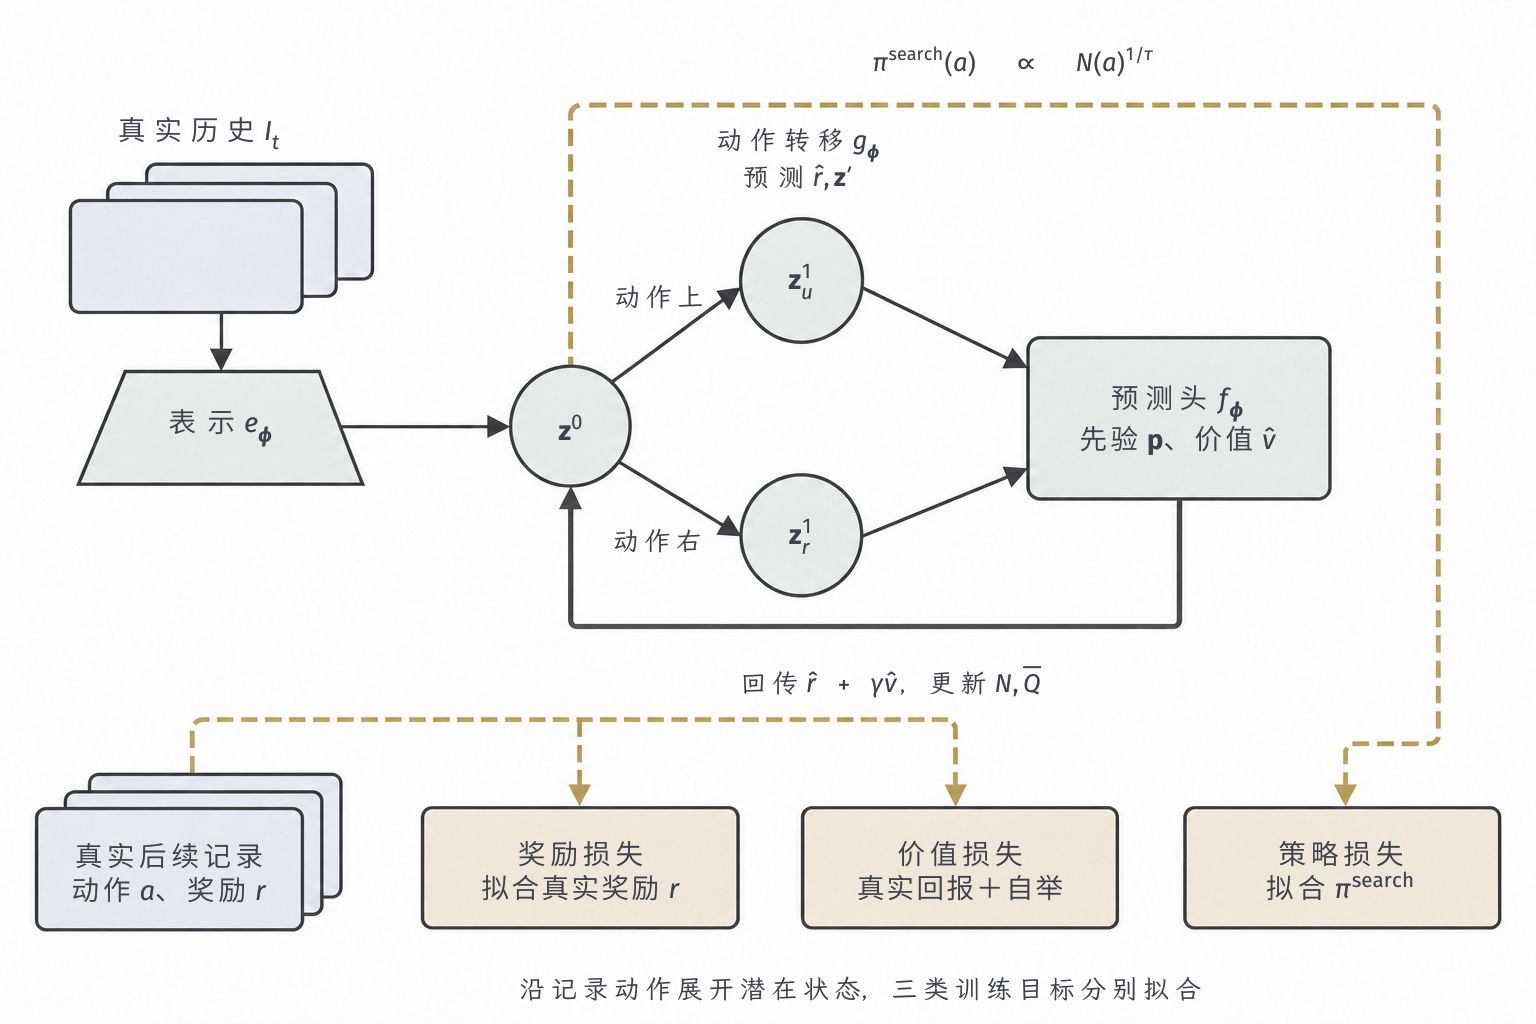
\includegraphics[width=157.400mm]{figures/10-reinforcement-learning/01-problems-and-solving/generated/rl-learning-muzero/figure.png}
  \caption{MuZero的搜索与学习。上部在潜在状态中展开并把边奖励加上折扣叶值传回根；下部用真实轨迹训练奖励与价值预测，用搜索访问分布训练策略先验。潜在后继不是新观测，访问分布也不是真实动作频率的简单重放。历史帧和搜索分支仅为示意，不固定历史长度或树规模。}
  \label{fig:rl-learning-muzero}
\end{figure*}

例如人工搜索快照中根节点先已有向右$N=2,\overline Q=0.85$，向上$N=1,\overline Q=0.6$；一次新展开给向右返回$0.68$，则其访问数变3、均值变$(2\times0.85+0.68)/3\approx0.7933$。若温度为1，四次访问对应策略目标$(3/4,1/4)$；温度趋于0时则集中到访问数最大的动作。这里的访问来自搜索模拟，不是环境在同一状态真实走了四步。

搜索得到的访问统计随后也用于训练网络。我们从真实回放取起点和后续动作，按记录动作展开$K$步：奖励头拟合真实奖励，价值头拟合真实奖励加末端搜索价值，策略头拟合搜索访问分布。令$\bm\pi^{\mathrm{search}}_{t+k}$为该时刻保存或重新计算的搜索策略目标，$z^V_{t+k}$为相应$n$步价值目标；下面的损失在各展开位置累加，按三类误差最小化模型参数：
\begin{align}
  z^V_t&=\sum_{j=0}^{n-1}\gamma^j r_{t+j}
                     +\gamma^n v^{\mathrm{search}}_{t+n}, \notag\\
  L_{\mathrm{MZ}}
    &=\sum_{k=0}^{K}
       \left[\ell_v(\widehat v^k,z^V_{t+k})
            -\sum_a\pi^{\mathrm{search}}_{t+k}(a)\log p^k_a\right]
      +\sum_{k=0}^{K-1}\ell_r(\widehat r^k,r_{t+k}).
  \label{eq:rl-learning-muzero-loss}
\end{align}
真实终止时截断奖励和自举；棋类可用最终胜负作为价值目标，Atari等还会使用变换后的离散价值表示。式中$r_{t+k}$仍是执行记录动作$a_{t+k}$后的奖励，不能把潜在展开的第一个奖励错位一格。优化损失更新三个模块；下一批真实交互再用新模块搜索，形成“搜索改进策略目标、网络拟合搜索结果”的循环。

训练中的策略目标来自搜索，价值与奖励目标又来自真实记录及末端估值。因此模型预测影响搜索，搜索影响下一批真实行为和训练目标，模型随后再拟合这些目标。搜索先验不是人工正确标签，而是这个反馈过程的一部分；模型在未验证的分支上出错时，搜索和学习也可能共同偏离真实任务。

EfficientZero针对有限真实交互训练样本补强这一循环：用记录后继的编码监督潜在展开的一致性，预测一段奖励的价值前缀以降低逐步奖励误差对备份的影响，并对旧策略轨迹记录的价值目标进行离策略修正和重新分析。以预测器$q$为例，一致性项可用
$-\operatorname{cos}(q(\widehat{\bm z}^{k}),\operatorname{sg}(e(o_{t+k})))$；
停止梯度使目标分支不被当前一致性损失同步更新，但它本身不能排除表示塌缩；实际稳定性还依赖完整训练设计。它是在MuZero搜索学习接口上提高已有交互记录的利用率，不是“增加一个重建头”就自动取得相同样本效率\scite{rl3-ye2021efficientzero}

表\ref{tab:rl-learning-model-requirements}将两种要求对照。一个模型在行为策略轨迹上准确预测价值，仍可能在很少训练过的动作组合和更深搜索中任意出错；因此“无需重建”免去的是一个输出要求，不是免去反事实检验。部署时MuZero仍主要依赖搜索访问统计选动作，单独取策略头最大值是另一个执行协议。

\begin{table*}[t]
  \centering
  \small
  \begin{tabularx}{\linewidth}{>{\raggedright\arraybackslash}p{26mm} >{\raggedright\arraybackslash}X >{\raggedright\arraybackslash}X}
    \toprule
    模型要求 & 直接训练或检查的对象 & 不能由此自动推出什么 \\
    \midrule
    可观测状态或图像重建 & 当前或未来可观测量的误差、似然 & 关键动作排序、未覆盖反事实及安全性 \\
    奖励、价值和策略预测 & 指定动作序列下的奖励、策略相关值及搜索分布 & 任意策略的回报、任意展开深度及完整环境规则 \\
    控制充分表示 & 在所需策略和干预集合上保留会影响动作选择的奖励或价值差别 & 超出这组策略、任务和干预后的继续有效性 \\
    \bottomrule
  \end{tabularx}
  \caption{重建与价值相关预测。要求应随模型实际承担的决策任务确定，不能按视觉精细程度排出统一优劣。}
  \label{tab:rl-learning-model-requirements}
\end{table*}

% Outline: 3.4.5
\subsection{潜在轨迹规划与价值引导}
\label{sec:rl-learning-tdmpc}

MuZero沿树分配离散分支的展开次数。连续动作下每个节点有无穷多候选，另一种接口是直接采样并优化短动作序列。TD-MPC将潜在动力学与TD价值结合：模型预测短段奖励和状态，末端评论家估计长尾回报，策略先验提出部分候选以缩小搜索范围。图\ref{fig:rl-learning-tdmpc}分开提议与执行，因为即使先验参与学习，最终动作仍由本轮规划评分决定。

\begin{figure*}[t]
  \centering
  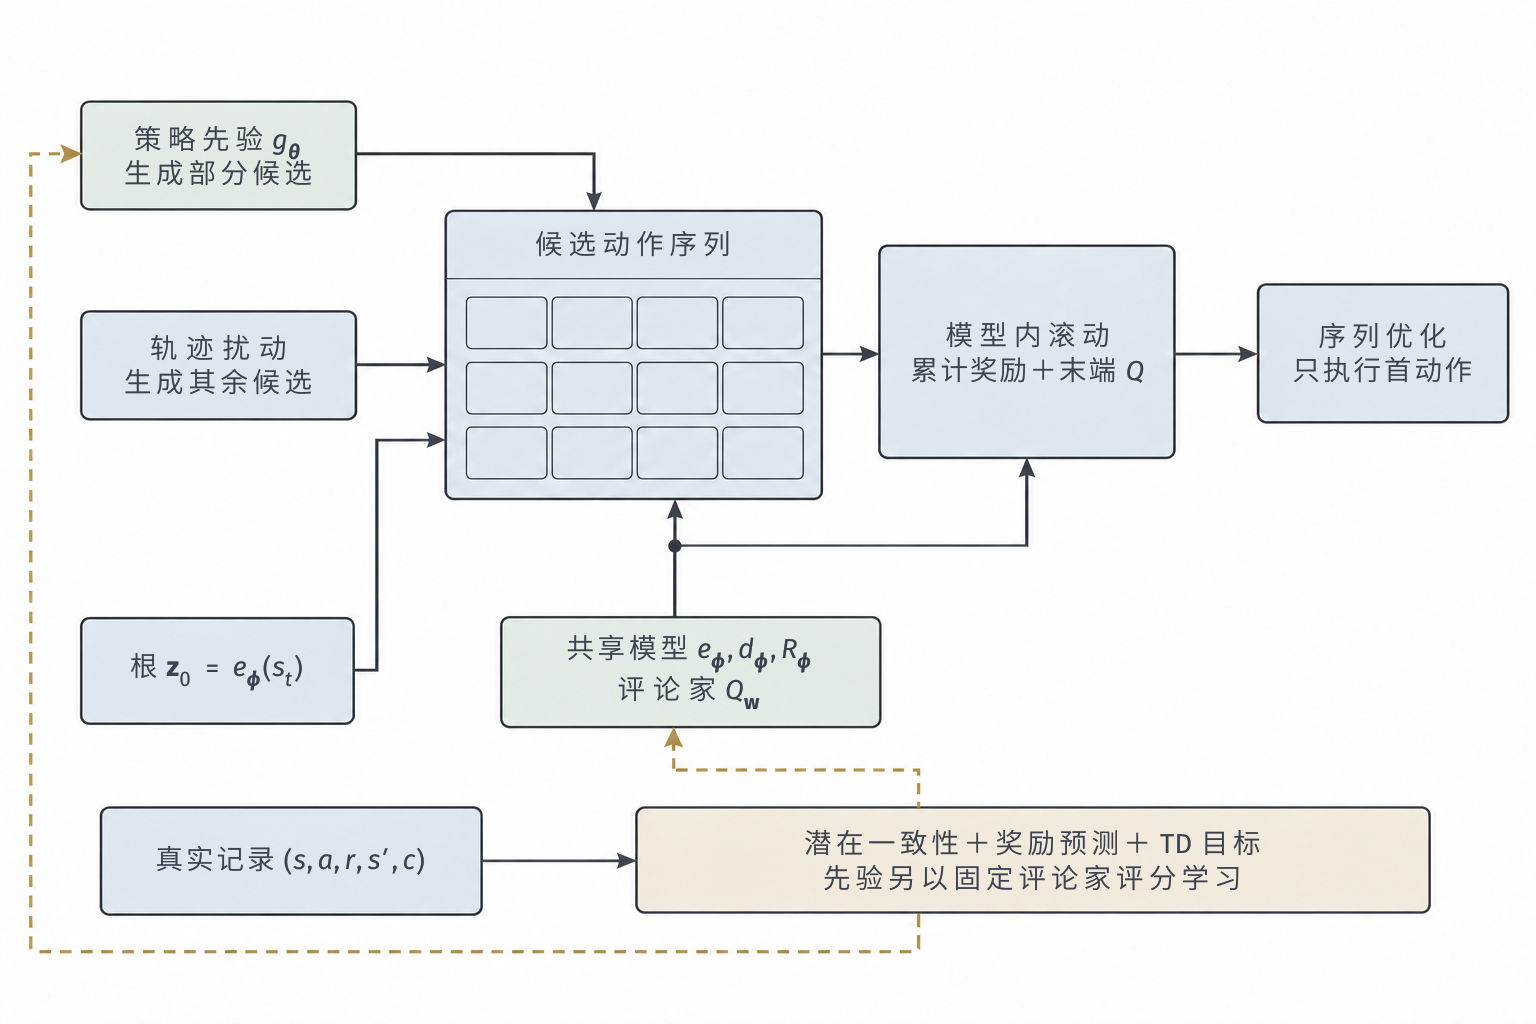
\includegraphics[width=157.400mm]{figures/10-reinforcement-learning/01-problems-and-solving/generated/rl-learning-tdmpc/figure.png}
  \caption{TD-MPC中的候选生成、模型评分与参数学习。各候选共享当前真实根；策略先验递归提出部分动作序列，其余候选由轨迹扰动形成。共享模型用于提议中的状态预测与候选评分，预测奖励累计后接末端Q；候选经回报加权或精英迭代优化后，只执行所求序列的首动作。训练虚线更新共享模型、评论家和先验参数，不指向某一条预测轨迹。轨迹格仅为示意，不规定候选数或规划时域。}
  \label{fig:rl-learning-tdmpc}
\end{figure*}

令策略先验的确定性动作映射为$g_{\bm\theta}$，其诱导策略为$\pi_{\bm\theta}(\mathrm da\mid\bm z)=\delta_{g_{\bm\theta}(\bm z)}(\mathrm da)$。先从当前真实状态编码$\bm z_0=e_{\bm\phi}(s)$，再按候选动作预测$\bm z_{j+1}=d_{\bm\phi}(\bm z_j,a_j)$。为了比较这些合法序列，评分累加前$L$步预测奖励，并在末端调用策略先验和评论家补上未展开部分：
\[
  \widehat F(a_{0:L-1})
  =\sum_{j=0}^{L-1}\gamma^j R_{\bm\phi}(\bm z_j,a_j)
      +\gamma^L Q_{\bm w}(\bm z_L,g_{\bm\theta}(\bm z_L)).
\]
上式先写规划片段内不终止的情形；有终止时，需像式\eqref{eq:rl-learning-mve}一样用继续标记屏蔽后续奖励和末端值。末端的$Q$已含末端动作的奖励，前面的和只到$L-1$，从而没有重复计数。候选可以混合高斯扰动序列与策略先验滚动；按回报加权或选精英迭代优化后，只执行首动作。即使先验在训练中不断提高，最终动作也未必等于$g_{\bm\theta}(\bm z_0)$。

真实短序列支持三类损失。用$\operatorname{sg}$表示停止梯度，以单步标量形式说明其关系：
\begin{align}
  y_t&=r_t+\gamma c_t
      Q_{\bar{\bm w}}(\bar{\bm z}_{t+1},
                             g_{\bm\theta}(\bar{\bm z}_{t+1})), \notag\\
  \ell_t&=\lambda_z\|
        d_{\bm\phi}(\bm z_t,a_t)-\operatorname{sg}(\bar{\bm z}_{t+1})
                              \|_2^2
       +\lambda_r(R_{\bm\phi}(\bm z_t,a_t)-r_t)^2 \notag\\
       &\quad+\lambda_Q(Q_{\bm w}(\bm z_t,a_t)
                                      -\operatorname{sg}(y_t))^2.
  \label{eq:rl-learning-tdmpc-loss}
\end{align}
\Needspace{14\baselineskip}
$\bar{\bm z}_{t+1}$由目标编码器对真实后继编码；多步训练时，预测分支沿记录动作递归展开，并按深度加权这些损失\scite{rl3-hansen2022tdmpc}
策略先验通过提高$Q(\bm z,g_{\bm\theta}(\bm z))$学习，优化它时需固定评论家参数；模型和价值训练则使用记录动作。目标网络、归一化、正则化及实际Q集合依具体版本而定，式\eqref{eq:rl-learning-tdmpc-loss}展示原始方法的核心接口，不是TD-MPC2全部实现细节。

TD-MPC2继续使用短潜在规划和末端价值，但对潜在状态做SimNorm归一化，采用离散分布式奖励与价值预测、Q集成和最大熵策略先验等设计来增强跨任务训练稳定性。若把向量分成多个小组，每组softmax后的分量非负且和为1，SimNorm便限制了潜在表示的尺度；这不等于获得了动力学误差的统计置信界。分布式目标改善不同奖励尺度的优化，Q集成抑制部分过估计，也不能替代真实访问覆盖。

TD-MPC2原论文报告104个在线任务、四类任务域，并另有多任务规模实验；其中317M参数、80任务的设置不能当成所有对比方法统一使用的预算。其结果支持的是相应交互训练记录、模型和任务协议下的经验结论，不是“潜在规划必然优于树搜索”的一般排序\scite{rl1-hansen2024-tdmpc2}

表\ref{tab:rl-learning-planning-budgets}按模型查询而不是名称比较三种接口。在固定总查询数$B$下，$N$条长度$L$、每条$M$粒子的轨迹大致消耗$NLM$次转移查询；树搜索可能每次模拟只扩展一个新节点，但还需遍历已建路径和维护统计。神经网络批处理、动作维数和叶值计算成本都不同，查询数相同仍不等于墙钟时间相同。

\begin{table*}[t]
  \centering
  \small
  \begin{tabularx}{\linewidth}{>{\raggedright\arraybackslash}p{23mm} >{\raggedright\arraybackslash}X >{\raggedright\arraybackslash}X >{\raggedright\arraybackslash}X}
    \toprule
    规划接口 & 主要查询模块 & 动作结构 & 预算分配 \\
    \midrule
    潜在树搜索 & 表示、动力学、奖励、策略先验、叶值 & 有限分支最直接；连续动作需额外候选机制 & 在重复访问的分支间分配展开，并复用树中统计 \\
    轨迹采样 & 动力学、奖励，可选末端价值 & 向量动作及显式约束便于联合采样 & 候选数、粒子数、时域和迭代轮数相互争用预算 \\
    价值引导短规划 & 潜在动力学、奖励、末端Q、策略先验 & 常用于连续控制 & 用评论家替代长尾滚动，把查询用于短轨迹优化 \\
    \bottomrule
  \end{tabularx}
  \caption{相同模型查询预算下仍需区分的计算。价值引导是轨迹评估的组成方式，可以与不同采样优化器组合。}
  \label{tab:rl-learning-planning-budgets}
\end{table*}

% Outline: 3.4.6
\subsection{模型偏差与规划边界}
\label{sec:rl-learning-model-bias}

验证集上的低平均误差未必保护规划动作，因为规划器查询模型的方式不是随机平均：它专门寻找预计回报最高的候选。当某个少覆盖分支被高估，增加搜索反而可能更稳定地找到它。这称为\term{模型利用偏差}（model exploitation），即优化器将预测错误当成可利用收益。图\ref{fig:rl-learning-model-exploitation}与下面的两路线例子展示了这一选择过程。

\begin{example}[优化器选择了最乐观的错误]
  \label{ex:rl-learning-model-exploitation}
  将网格局部改成两个可选路线的独立教学任务。安全路线的真实与预测回报都为$0.6$；稀少访问的“捷径”进入终点的真实概率为$0.1$，失败进入零回报吸收态，即真实回报$0.1$。模型却把成功概率估为$0.9$，于是预计回报$0.9$并反复选择捷径。
  若测试转移样本所代表的路线分布有$99\%$质量落在安全路线，则按该分布计算的平均绝对回报误差仅为$0.01\times0.8=0.008$，实际选择的动作却损失$0.5$。
  增加规划候选数可以更稳定地选中这个错误最大值，并不会自动降低误差。
\end{example}

\begin{figure}[htbp]
  \centering
  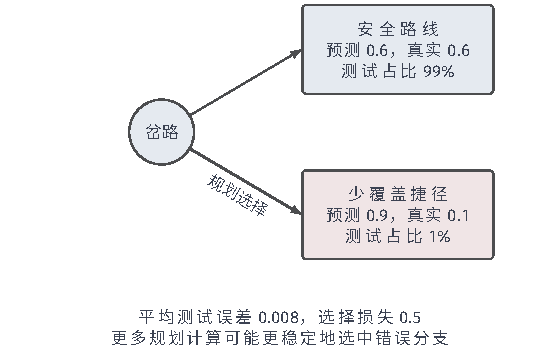
\includegraphics[width=94.749mm]{figures/10-reinforcement-learning/01-problems-and-solving/tikz/rl-learning-model-exploitation.pdf}
  \caption{少覆盖分支上的模型利用偏差。数字属于例\ref{ex:rl-learning-model-exploitation}的人工两路线任务；模型内最优动作与真实最优动作相反，测试分布的低平均误差掩盖了这一差别。}
  \label{fig:rl-learning-model-exploitation}
\end{figure}

要把模型误差变成价值误差，需要说明误差在哪些状态动作上受控。下面给出一个统一但较强的条件；它不需要模型来自某种特定学习算法，也不会从经验损失小自动成立。

\begin{theorem}[固定策略的模型误差界]
  \label{thm:rl-learning-simulation}
  在相同有限状态动作空间、折扣$0\leq\gamma<1$上，两个MDP的奖励均值为$R,\widehat R$、转移核为$T,\widehat T$。假设两者奖励均值绝对值均不超过$R_{\max}$，并且对每个合法$(s,a)$，
  \[
    |R(s,a)-\widehat R(s,a)|\leq\varepsilon_R,\qquad
    \sum_{s'}|T(s'\mid s,a)-\widehat T(s'\mid s,a)|
       \leq\varepsilon_T.
  \]
  对任意固定平稳策略$\pi$，记两个模型中的价值为$V^\pi,\widehat V^\pi$，则
  \begin{equation}
    \|V^\pi-\widehat V^\pi\|_\infty
       \leq B_{\mathrm{model}}
       :=\frac{\varepsilon_R}{1-\gamma}
        +\frac{\gamma R_{\max}\varepsilon_T}{(1-\gamma)^2}.
    \label{eq:rl-learning-simulation-bound}
  \end{equation}
  在相同初始分布下，$|J(\pi)-\widehat J(\pi)|$也不超过$B_{\mathrm{model}}$。
\end{theorem}

\begin{proof}
  对策略动作取平均后，奖励误差仍不超过$\varepsilon_R$，每一行转移分布的$L^1$误差仍不超过$\varepsilon_T$。由奖励界，
  $\|\widehat V^\pi\|_\infty\leq R_{\max}/(1-\gamma)$。
  相减两个Bellman方程，并加减$\gamma T^\pi\widehat V^\pi$，得到
  \[
    V^\pi-\widehat V^\pi
     =R^\pi-\widehat R^\pi
       +\gamma T^\pi(V^\pi-\widehat V^\pi)
       +\gamma(T^\pi-\widehat T^\pi)\widehat V^\pi .
  \]
  因$T^\pi$是随机矩阵，其中间项的无穷范数至多为
  $\gamma\|V^\pi-\widehat V^\pi\|_\infty$。对末项逐行用三角不等式，
  \[
    \|(T^\pi-\widehat T^\pi)\widehat V^\pi\|_\infty
      \leq\varepsilon_T\|\widehat V^\pi\|_\infty
      \leq\frac{R_{\max}\varepsilon_T}{1-\gamma}.
  \]
  合并三项并把带$\gamma$的价值差移到左边，即得式\eqref{eq:rl-learning-simulation-bound}。最后对相同$\mu_0$取期望，概率加权平均不超过无穷范数，得到回报差结论。
\end{proof}

这种论证通常称为模拟引理的一个形式。这里$\varepsilon_T$是$L^1$误差；若用总变差$\operatorname{TV}=\tfrac12\|\cdot\|_1$定义误差，转移项系数必须相应改变，不能直接抄同一个常数。原始有限MDP学习分析中的模拟论证也是把局部模型误差传到长期回报，但具体时域与误差规范应按所引用结果区分\scite{rl3-kearns2002efficient}

固定策略误差界还能支持模型内选出的策略，但需要误差条件统一覆盖候选所需的全部状态动作。设规划在学习模型的合法策略中最大化$\widehat J$，输出$\widehat\pi$的次优度至多$\epsilon_{\mathrm{plan}}$。若上述统一误差事件成立，模型界就同时适用于真实最优策略和依据模型训练记录选出的$\widehat\pi$。将真实性能差拆成两侧模型误差和中间规划误差，得到
\begin{align*}
  J(\pi^*)-J(\widehat\pi)
   &=J(\pi^*)-\widehat J(\pi^*)
     +\widehat J(\pi^*)-\widehat J(\widehat\pi)
     +\widehat J(\widehat\pi)-J(\widehat\pi)\\
   &\leq 2B_{\mathrm{model}}+\epsilon_{\mathrm{plan}}.
\end{align*}
中间项利用了$\widehat J(\pi^*)\leq\max_\pi\widehat J(\pi)$。若仅知道某个固定行为策略的模型误差小，第一和第三项不能同时这样控制，尤其不能把训练之后挑出的策略当成预先固定的策略。

表\ref{tab:rl-learning-model-validity}归纳了检验层次。更精细的分析可以按占用分布加权误差，减少统一界的保守性，但要补上策略覆盖或分布转移的控制。重建误差、模型似然和集成分歧都可能是有用诊断量；它们各自需要通往决策目标的论证。基于模型置信集合的鲁棒优化与风险约束留到第\ref{chap:rl-trustworthy}章。

\begin{table*}[t]
  \centering
  \small
  \begin{tabularx}{\linewidth}{>{\raggedright\arraybackslash}p{24mm} >{\raggedright\arraybackslash}X >{\raggedright\arraybackslash}X}
    \toprule
    检验层次 & 它回答的问题 & 仍需补充的条件 \\
    \midrule
    重建质量 & 已观察内容能否编码并还原 & 决策相关量是否保留、历史是否充分 \\
    预测一致性 & 已覆盖动作序列的预测是否吻合 & 更长滚动、策略变化及误差校准 \\
    反事实正确性 & 换动作后模型是否仍有效 & 对所需干预的真实覆盖或可识别结构 \\
    控制充分性 & 用该表示和模型是否保持所需策略的决策质量 & 具体任务、策略类、规划深度与误差到性能的联系 \\
    \bottomrule
  \end{tabularx}
  \caption{模型质量不是一个无条件通用的分数。前一行通过并不自动保证后一行通过。}
  \label{tab:rl-learning-model-validity}
\end{table*}

% Outline: 3.5
\section{基于模型的策略优化}
\label{sec:rl-learning-model-policy}

当前规划只为这次状态求一个动作或动作序列，下次仍需重新搜索。若要训练一份可以跨状态重复调用的策略，优化变量就从本轮$a_{0:L-1}$改成共享参数$\bm\theta$。模型可以让回报梯度经过预测动力学传到策略，也可以生成经验供行动者—评论家训练。两者都将大量计算放在训练阶段，部署动作主要来自训练后的策略；但策略读取的状态仍可能需要模型依据新观测推断。

% Outline: 3.5.1
\subsection{模型梯度与策略搜索}
\label{sec:rl-learning-model-gradient}

先考察模型如何提供真实环境无法直接给出的导数。在连续控制中，策略改变本步动作，动作改变后继状态，后继又改变下一次策略输出；求导需要保留整条依赖。先用一个只有两步的系统观察这些路径，再写一般递推。

\begin{example}[两步模型梯度]
  \label{ex:rl-learning-two-step-gradient}
  将连续控制简化为无噪声标量系统$x_{t+1}=ax_t+bu_t$，$u_t=\theta x_t$，固定$x_0=1$，仅有末端成本$C=x_2^2/2$。记$q=a+b\theta$，则$x_1=q$、$x_2=q^2$，所以
  \[
    \frac{\partial x_1}{\partial\theta}=b,\qquad
    \frac{\partial x_2}{\partial\theta}
       =q b+b x_1=2bq,\qquad
    \frac{\partial C}{\partial\theta}=2bq^3.
  \]
  人工取$a=b=1,\theta=-0.5$，梯度为$0.25$；学习率$0.1$的一次成本下降更新给$\theta'=-0.525$。若在第二步把输入状态$x_1$整体停止求导，便会丢掉上式的$q b$项，只留下本步参数直接改变动作的$b x_1$项，成本梯度变为$0.125$，恰好少一半。仅漏掉第二次策略调用中的状态导数并不等于这个操作，因为动力学对$x_1$的直接依赖仍可传回梯度。
\end{example}

设学到的动力学可重参数化为
$\bm x_{t+1}=f_{\bm\phi}(\bm x_t,\bm u_t,\bm\xi_t)$，策略为
$\bm u_t=g_{\bm\theta}(\bm x_t)$，$\bm\xi_t$是分布与策略参数无关的随机噪声。这里$g_{\bm\theta}$是确定性动作映射，其诱导策略是$\pi_{\bm\theta}(\mathrm du\mid\bm x)=\delta_{g_{\bm\theta}(\bm x)}(\mathrm du)$。固定模型参数$\bm\phi$并对一条采样轨迹求导，记
$\bm D_t=\partial\bm x_t/\partial\bm\theta$。由链式法则，
\begin{equation}
  \bm D_{t+1}
   =\left(f_{\bm x}+f_{\bm u}g_{\bm x}\right)\bm D_t
       +f_{\bm u}g_{\bm\theta},\qquad \bm D_0=\bm0.
  \label{eq:rl-learning-model-chain}
\end{equation}
这里$f_{\bm x},f_{\bm u}$分别是动力学对状态、动作的Jacobian，$g_{\bm x},g_{\bm\theta}$分别是策略对状态、参数的Jacobian，均在当前滚动状态、动作和噪声上计算。第二项是本步参数直接改变动作的影响，第一项保留先前动作经状态传来的影响。把这些敏感度乘上成本导数，就能得到模型内策略的下降方向。若有限时域成本为
$C(\bm\theta)=\mathbb E\sum_{t=0}^{L-1}c(\bm x_t,\bm u_t)+
\mathbb E c_L(\bm x_L)$，则
\[
 \nabla_{\bm\theta}C
  =\mathbb E\left[
    \sum_{t=0}^{L-1}
      \left(\bm D_t^\top\nabla_{\bm x}c_t+
       (g_{\bm x}\bm D_t+g_{\bm\theta})^\top
                                       \nabla_{\bm u}c_t\right)
          +\bm D_L^\top\nabla c_L(\bm x_L)\right].
\]
这里成本越小越好，与本章奖励最大化的关系是$r_t=-c_t$。将导数移入期望需要可微性和可积控制；接触、碰撞、离散动作及硬终止并不会自动满足这些条件。图\ref{fig:rl-learning-model-gradient}区分了训练模型与借模型训练策略的两条路径。

\begin{figure*}[t]
  \centering
  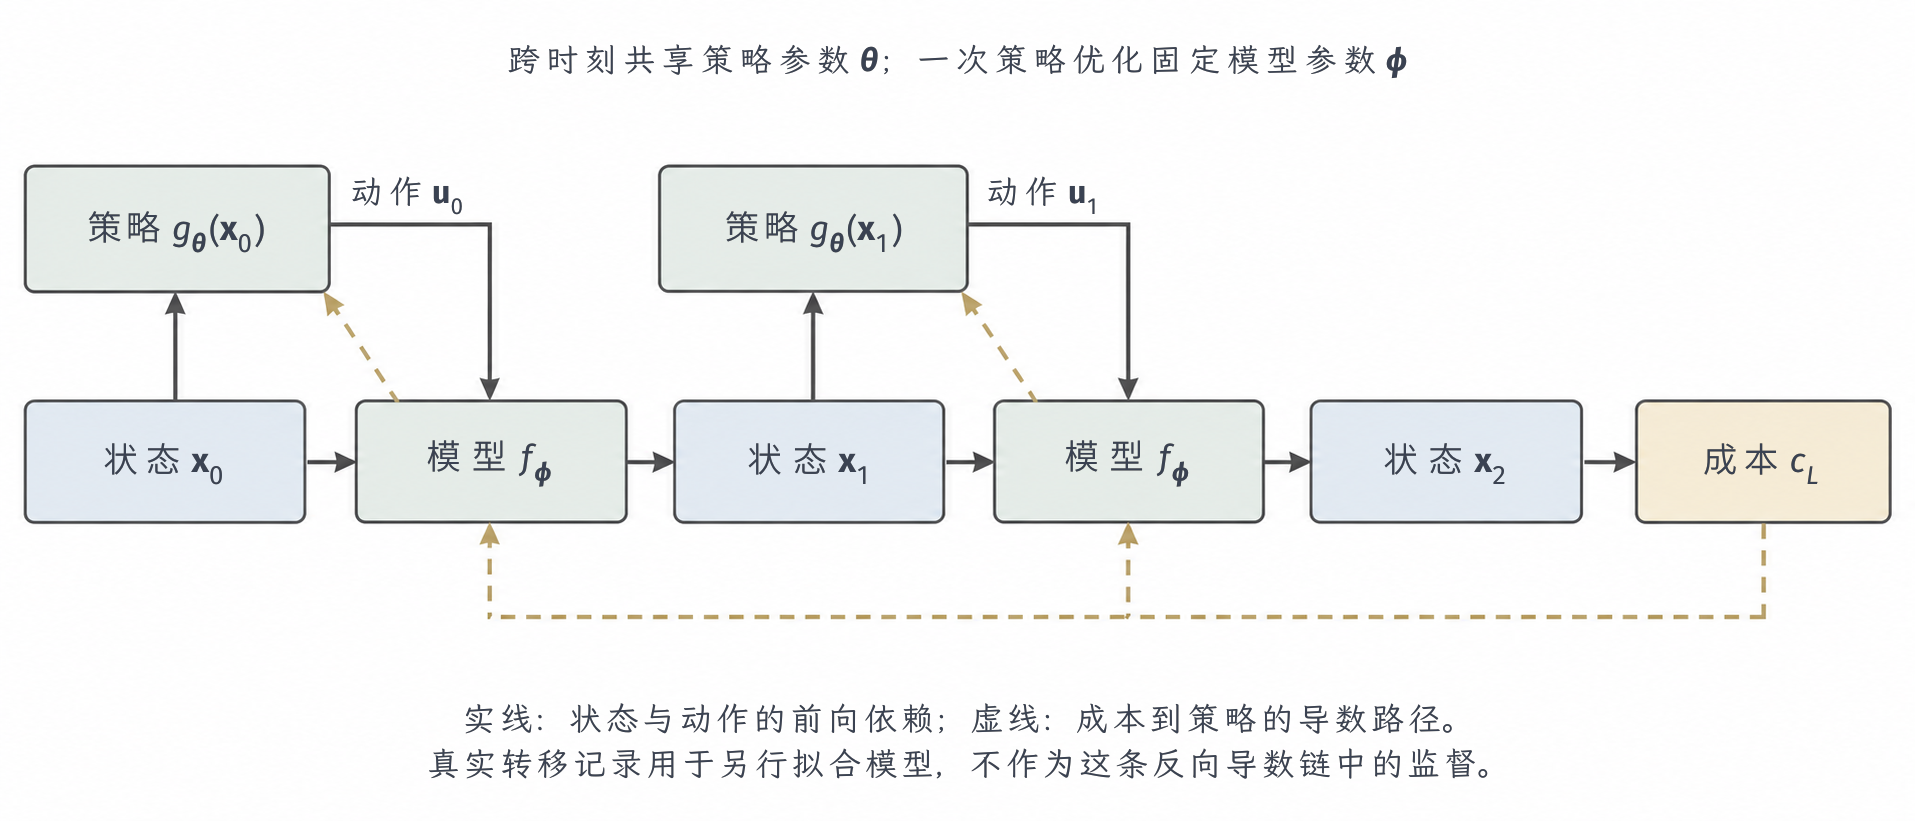
\includegraphics[width=157.400mm]{figures/10-reinforcement-learning/01-problems-and-solving/generated/rl-learning-model-gradient/figure.png}
  \caption{模型中的策略展开。每个时刻调用同一组策略参数，后继状态又进入策略；实线为前向依赖，虚线为策略优化时的反向导数。模型参数由真实转移训练记录更新，在一次策略梯度计算中固定，不因允许梯度穿过模型就同时最小化模型预测损失。}
  \label{fig:rl-learning-model-gradient}
\end{figure*}

一般递推正好包含刚才两步例中的两种影响。$\bm D_t$保存此前参数变化已经造成的状态变化；本步又通过$g_{\bm\theta}$直接改变动作。旧状态变化一方面通过动力学的$f_{\bm x}$传向后继，另一方面先改变本步策略输出，再通过$f_{\bm u}g_{\bm x}$传向后继。把这两条旧影响与本步新影响相加，才不会漏掉后续策略对输入状态的依赖。

采样路径求导需要处理随机轨迹；另一种方式是直接传播状态分布的近似参数。PILCO使用高斯过程描述动力学增量，同时保留给定动力学训练记录后的均值预测和不确定性。给定近似高斯的状态分布与参数策略，它通过矩匹配，让近似分布的均值和协方差等于所算的后继矩，递推状态分布，再对期望长期成本求导。把分布参数合记为
$\bm m_t=(\bm\mu_t,\operatorname{vec}\bm\Sigma_t)$，递推写成
$\bm m_{t+1}=F_{\bm\phi}(\bm m_t,\bm\theta)$，则
\[
 \frac{\partial\bm m_{t+1}}{\partial\bm\theta}
  =\frac{\partial F_{\bm\phi}}{\partial\bm m_t}
       \frac{\partial\bm m_t}{\partial\bm\theta}
       +\frac{\partial F_{\bm\phi}}{\partial\bm\theta}.
\]
期望成本$\bar c(\bm m_t)$的导数再乘这些敏感度。高斯近似使计算可行，却可能丢失多峰分布；高斯过程后验不确定性也依赖核和噪声假设。这个过程不是对真实非线性轨迹分布的精确积分\scite{rl3-deisenroth2011pilco}

模型也可作为黑盒评分器。固定$\bm\theta$，用它在模型里产生完整行为，再以采样回报驱动第\ref{sec:rl-learning-regularized-search}节的搜索；这不要求动力学可微，但需要更多候选评估。表\ref{tab:rl-learning-model-gradient-interfaces}对比所需的奖励查询、模型导数与随机变量密度。

\begin{table*}[t]
  \centering
  \small
  \begin{tabularx}{\linewidth}{>{\raggedright\arraybackslash}p{25mm} >{\raggedright\arraybackslash}X >{\raggedright\arraybackslash}X}
    \toprule
    接口 & 需要模型提供什么 & 主要计算与误差来源 \\
    \midrule
    采样路径反向传播 & 可微转移、奖励和策略；噪声可重参数化或另作梯度估计 & 保存或重算长度$L$的展开，导数连乘可能消失或爆炸；采样方差与模型导数偏差 \\
    分布传播的解析近似 & 可计算的分布矩、期望成本及其导数 & 传播均值和协方差；对分布形状、核和成本形式有要求，矩近似引入偏差 \\
    黑盒策略搜索 & 候选参数对应的模型回报样本 & 多候选、多噪声重复评分；不需模型Jacobian，仍会利用错误的回报排序 \\
    \bottomrule
  \end{tabularx}
  \caption{模型参与策略搜索的三种方式。可微性减少了部分搜索成本，但给模型增加了导数质量要求。}
  \label{tab:rl-learning-model-gradient-interfaces}
\end{table*}

预测误差小和导数准确是两件事。例如真实一步模型$f(u)=u$，近似模型
$\widehat f(u)=u+\epsilon\sin(\omega u)$，全域预测误差不超过$\epsilon$，而导数误差为$\epsilon\omega\cos(\omega u)$，可随$\omega$任意增大。在$u=0$两者输出甚至完全相同。前节的价值误差界控制函数值，不控制这个导数；借模型求梯度还应检查策略会用到的局部敏感度，或用真实交互的回报记录检验更新是否确实改进。

% Outline: 3.5.2
\subsection{想象轨迹中的行动者—评论家}
\label{sec:rl-learning-dreamer}

模型不必只提供导数，也可以在昂贵真实交互之间反复产生策略训练轨迹。World Models将观测编码为潜在变量，用循环模型预测后继，并在模型内搜索控制器参数。Dreamer则将这个训练环境接到行动者—评论家：策略在模型中行动，评论家评价预测回报，行动者再根据评价改进。这样复用的是学习到的预测规律，而不是新增真实证据\scite{rl3-ha2018worldmodels}

模型内训练可先按三个阶段理解。真实轨迹提供观测、动作和结果，用来训练模型；从其中一个已有观测历史推断当前内部状态，再让固定模型模拟若干步，形成策略训练材料；最后把策略拿回真实环境测试。模拟中看见的是模型预测，只有重新执行真实动作才会增加环境证据。“想象”指这段不再读取未来真实观测的模拟，不指随意编造与动作无关的画面。

\begin{definition}[想象轨迹]
  \label{def:rl-learning-imagination}
  给定一段真实观测与动作历史，先按模型的潜在后验抽取起点，再由固定的潜在转移模型和策略逐步生成后继潜变量与动作，并由预测头给出奖励和继续概率。这个模型内序列称为想象轨迹。后验属于拟合的潜在模型，不是未经证明就等于真实环境隐状态的条件分布；离开起点后没有新观测时，后继按模型先验生成，不能读取未来真实观测的编码。
\end{definition}

要区分真实起点与想象后继，需要明确模型在有观测和无观测时怎样更新。循环状态空间模型（RSSM）用确定性记忆保存历史递推，用随机潜变量表示当前状态的条件不确定性。为避免与真实历史$I_t$混用，分别记为$\bm m_t,\bm z_t$，合状态为$\bm x_t=(\bm m_t,\bm z_t)$。真实序列用观测更新后验；想象时没有新观测，只能从先验预测前进。仍把执行动作$a_t$后得到的奖励记为$r_t$：
\begin{align}
 \bm m_{t+1}&=f_{\bm\phi}(\bm m_t,\bm z_t,a_t),\notag\\
 q_{\bm\phi}(\bm z_{t+1}\mid\bm m_{t+1},o_{t+1})
       &\quad\text{用于真实观测序列的后验推断},\notag\\
 p_{\bm\phi}(\bm z_{t+1}\mid\bm m_{t+1})
       &\quad\text{用于无后续观测的先验滚动}.
 \label{eq:rl-learning-rssm}
\end{align}
奖励$r_t$及是否继续$c_t$的预测可在该转移的后继潜在状态上读出。若实现把进入状态时的奖励记作$r_{t+1}$，只须整体对齐索引，不能把旧观测之后、动作之前的奖励混进同一个目标。

这里的先验与后验比较的是同一个潜在状态。动作后、尚未看到$o_{t+1}$时，$p_{\bm\phi}$依据已有记忆预测它；看到新观测后，$q_{\bm\phi}$再用观测修正判断。真实序列能学习这种修正，无观测的想象序列只能使用预测。模型训练需要让预测接近带观测的修正，才可能从真实起点继续滚动；两者都是学习模型中的分布，不能直接认作真实隐藏状态分布。

真实序列中的观测、奖励和继续变量提供预测监督，但只有这三项还不足以训练无观测滚动：模型还需使先验接近带观测的后验。以DreamerV3的离散潜变量为例，记$q_t,p_t$为同一时刻的后验、先验。下面先累加三类负对数似然，再用分别停止一侧梯度的KL项训练先验和表示；模型参数最小化其真实序列期望：
\begin{align}
 \ell_{\mathrm{pred},t}
   &=-\log p_{\bm\phi}(o_t\mid\bm x_t)
     -\log p_{\bm\phi}(r_{t-1}\mid\bm x_t)
     -\log p_{\bm\phi}(c_{t-1}\mid\bm x_t),\notag\\
 \ell_{\mathrm{dyn},t}
   &=\max\{1,D_{\mathrm{KL}}(\operatorname{sg}(q_t)\|p_t)\},\notag\\
 \ell_{\mathrm{rep},t}
   &=\max\{1,D_{\mathrm{KL}}(q_t\|\operatorname{sg}(p_t))\},\notag\\
 L_{\mathrm{model}}&=\mathbb E\sum_t
       [\ell_{\mathrm{pred},t}+\ell_{\mathrm{dyn},t}
                         +0.1\ell_{\mathrm{rep},t}].
 \label{eq:rl-learning-dreamer-model}
\end{align}
序列首项没有对应转移监督时省去奖励和继续损失。这里$r_{t-1}$明确指进入$\bm x_t$的上一步奖励，并未改动本章的经验定义。两项KL分别调整先验和表示。nat是采用自然对数时熵与KL散度的计量单位，$1$ nat等于$1/\log2$ bit；这里的阈值1按该尺度计量散度。KL低于1 nat时，上述最大值取常数1，不再施加这项KL梯度压力；实际离散分布还混入$1\%$均匀概率以避免极端概率。观测重建帮助训练表示，但不能单独证明其对所有控制干预充分。

\begin{figure*}[t]
  \centering
  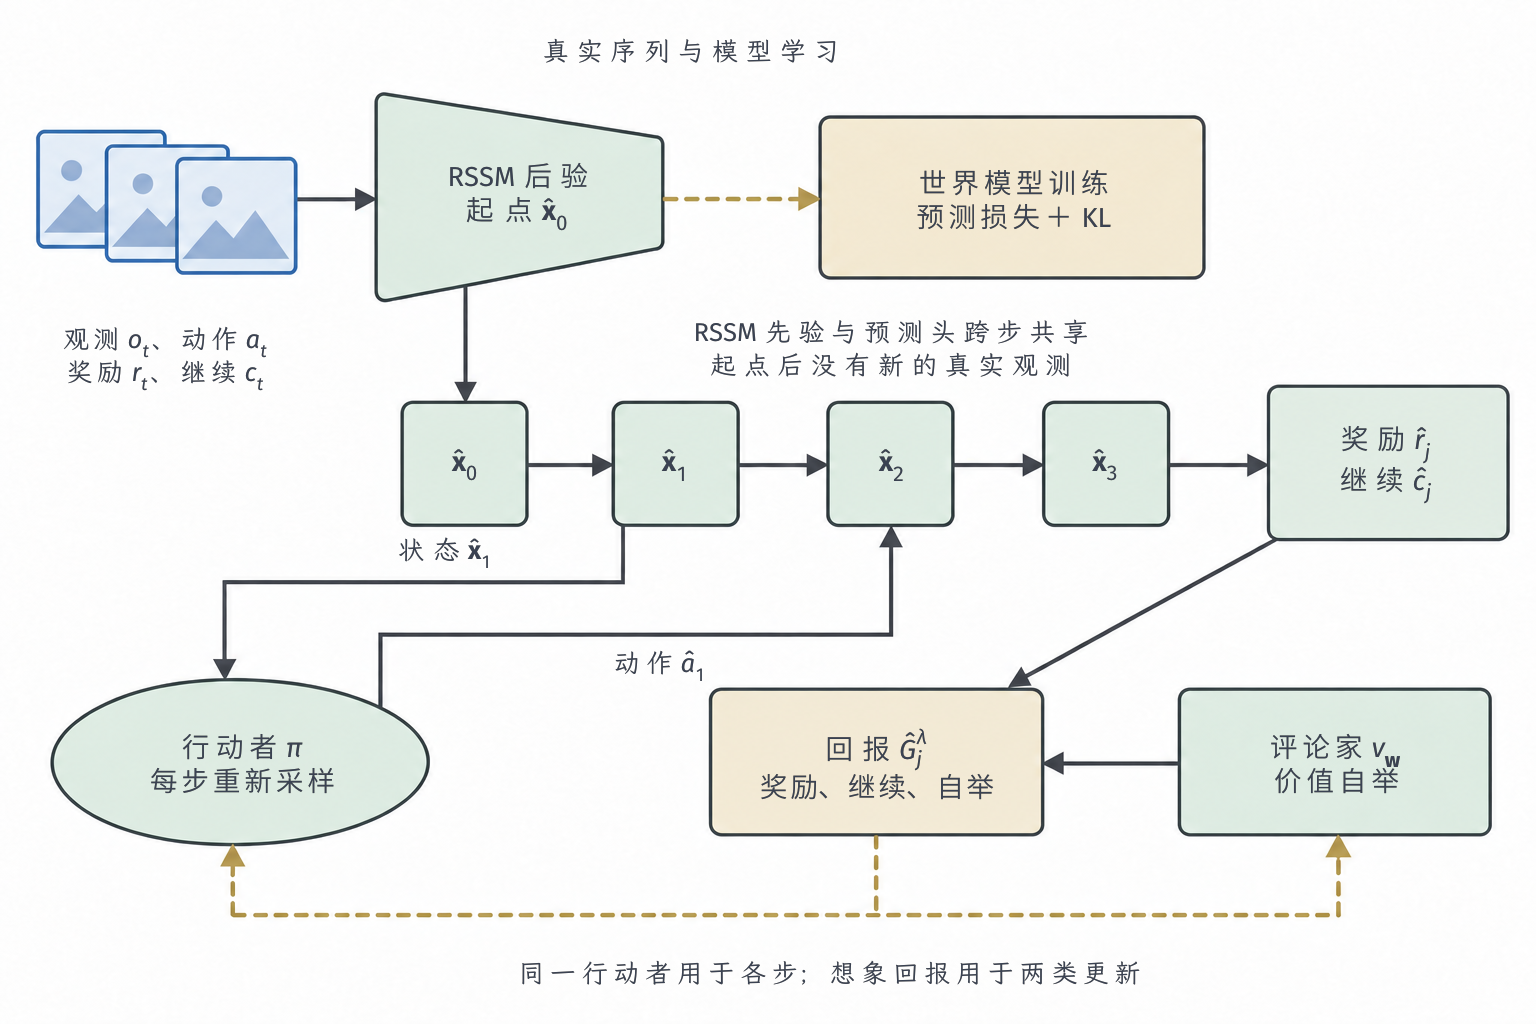
\includegraphics[width=157.400mm]{figures/10-reinforcement-learning/01-problems-and-solving/generated/rl-learning-dreamer/figure.png}
  \caption{RSSM上的真实学习与想象学习。真实序列经后验形成起点并训练世界模型；想象轨迹由先验前进，奖励和继续概率进入回报，价值给出末端自举。部署仍需用新观测更新模型状态，不能把“无逐步搜索”理解为“不再调用模型”。所示潜在格仅解释跨步复用与时序，不固定想象时域或状态维数。}
  \label{fig:rl-learning-dreamer}
\end{figure*}

模型固定后，行动者和评论家需要一个不再依赖未来真实奖励的训练目标。我们从真实后验状态$\widehat{\bm x}_0$开始想象，采样
$\widehat a_j\sim\pi_{\bm\theta}(\cdot\mid\widehat{\bm x}_j)$，再依次得到
$\widehat{\bm x}_{j+1},\widehat r_j,\widehat c_j$。记
$\widehat\gamma_j=\gamma\widehat c_j$为单步有效折扣，长度$L$的$\lambda$回报按逆序递推：
\begin{equation}
 \widehat G_L^\lambda=v_{\bm w}(\widehat{\bm x}_L),\qquad
 \widehat G_j^\lambda
  =\widehat r_j+\widehat\gamma_j
     [(1-\lambda)v_{\bm w}(\widehat{\bm x}_{j+1})
                              +\lambda\widehat G_{j+1}^\lambda].
 \label{eq:rl-learning-dreamer-return}
\end{equation}
例如教学设定$\gamma=0.9,\lambda=0.5,L=2$，两次继续概率均为1，
奖励为$(0.2,0.3)$，后继价值为$(0.4,0.6)$。于是
$\widehat G_1^\lambda=0.84$，
$\widehat G_0^\lambda=0.758$。若第二步继续概率改成0，则相应两值为$0.3$和$0.515$。这说明继续预测错误会同时污染回报与轨迹的有效权重。

Dreamer各版本使用同一训练分工，但不是同一损失。最初版本用连续随机潜变量，并在连续控制中通过模型和评论家反向传播想象回报来训练行动者。DreamerV2改用离散潜变量和直通估计，行动者结合路径导数与似然比估计的方式依动作类型、配置而异\scite{rl3-hafner2020dreamer}

V2的变化使离散视觉控制中的想象学习更实用，但不能据此把后续V3的纯似然比行动者写成相同梯度。V2的网络、目标与评估协议应按其独立论文理解\scite{rl3-hafner2021dreamerv2}

离散潜变量在前向计算中抽出离散取值，抽样操作本身没有通常的连续导数。直通估计（straight-through estimator）在反向计算时用一个连续代理的导数传递梯度，相当于为这一步另定求导规则。它使训练可执行，但一般是有偏估计；不能因为前向样本确实来自离散分布，就将反向代理称为精确导数。区分它与REINFORCE，有助于理解Dreamer不同版本怎样训练行动者。

V3还需处理不同任务的奖励尺度。本书采用2025年Nature正式版的表示：奖励和价值输出固定支撑上的离散概率，而不是直接回归一个标量。取
$b_i=\operatorname{symexp}(u_i)$，
$\operatorname{symexp}(u)=\operatorname{sign}(u)(e^{|u|}-1)$，$u_i$在$[-20,20]$上等距。若目标$y$位于$b_i,b_{i+1}$之间，two-hot目标把概率
$(b_{i+1}-y)/(b_{i+1}-b_i)$和
$(y-b_i)/(b_{i+1}-b_i)$放在相邻两点，其他为0；超出支持范围的值截到边界。训练用该目标与预测分布的交叉熵，读出的均值是$\sum_i p_i b_i$。它是在原始值域插值，不是“先在symlog域求均值，再反变换”的旧式概括。

two-hot编码将目标夹在相邻两点之间的距离转成两个概率，避免只指定最近的一个支撑点。用$\mathcal T(y)$记这一编码，评论家通过最小化它与预测分布的交叉熵拟合停止求导的想象回报，主要项为
\[
  \ell_{\mathrm{critic},j}
    =-\sum_i\mathcal T_i(\operatorname{sg}\widehat G_j^\lambda)
                   \log p_{\bm w,i}(\widehat{\bm x}_j).
\]
这里对软目标取交叉熵。正式版还用EMA评论家输出作正则，并加入真实回放上的辅助价值损失，权重为$0.3$；真实序列的目标利用对应想象起点的在策略回报作标注。这不同于把所有回报自举值统一替换为EMA目标网络。式\eqref{eq:rl-learning-dreamer-return}明确使用当前评论家，监督目标一侧停止梯度。

评论家拟合预测回报后，V3用回报减价值形成行动者优势，并对离散和连续动作均采用归一化的REINFORCE，而非让梯度直接穿过想象动力学。记
$W_j=\prod_{i<j}\widehat\gamma_i$，$c_{\mathrm{ret}}$为想象回报第95与第5百分位差的指数移动平均，则其最大化目标的采样形式为
\begin{equation}
 \sum_{j=0}^{L-1}W_j\left[
   \log\pi_{\bm\theta}(\widehat a_j\mid\widehat{\bm x}_j)
   \operatorname{sg}\left(
       \frac{\widehat G_j^\lambda-v_{\bm w}(\widehat{\bm x}_j)}
            {\max(1,c_{\mathrm{ret}})}\right)
     +\eta\,H(\pi_{\bm\theta}(\cdot\mid\widehat{\bm x}_j))
                       \right].
 \label{eq:rl-learning-dreamer-actor}
\end{equation}
状态、权重和优势在这次行动者更新中作为采样量固定，熵项鼓励而不是惩罚随机性。它从回放起点训练有限想象片段，是实际优化代理，不应声称未经校正就等于真实初始分布目标$J$的精确梯度；因此这里也没有用未归一化的采样和冒充归一化占用期望。

V3正式论文报告多个控制基准上的实验，多数基准使用5个训练种子；Minecraft与BSuite使用10个。Minecraft实验的动作包含抽象合成命令，且有加速破坏方块等协议约定。算法的真实环境证据应连同这些条件解读，不能只把“获得钻石”四字当成跨接口可比的性能单位\scite{rl1-hafner2025-dreamerv3}

表\ref{tab:rl-learning-imagination-cost}说明训练和部署的差别。图\ref{fig:rl-learning-dreamer}中的后验是观测历史的压缩推断，其何时能充当决策状态留给第\ref{chap:rl-information}章；算法把它作为行动者和评论家的潜在状态输入，其充分性需要额外验证。

\begin{table*}[t]
  \centering
  \small
  \begin{tabularx}{\linewidth}{>{\raggedright\arraybackslash}p{24mm} >{\raggedright\arraybackslash}X >{\raggedright\arraybackslash}X}
    \toprule
    阶段 & 模型及策略调用 & 不能省略的成本或检验 \\
    \midrule
    真实序列训练 & 编码观测、后验推断、重建及预测头，梯度更新模型 & 真实交互记录数量、序列长度与反向传播内存 \\
    想象训练 & 多起点先验滚动，逐步调用行动者、奖励、继续与价值头 & 模型转移数、评论家和行动者更新数；高模型回报需真实评估 \\
    部署执行 & 更新循环记忆和观测后验，从策略采样或取约定动作 & 每步状态推断仍有模型成本；随机或确定性评估须预先固定 \\
    在线再学习 & 将新经验写回回放并交替更新三个模块 & 是否允许继续交互、何时更新及更新后状态重算 \\
    \bottomrule
  \end{tabularx}
  \caption{想象学习没有消除模型计算，而是改变了计算发生的位置。部署不做候选轨迹搜索，也不等于一个无状态的策略网络即可运行。}
  \label{tab:rl-learning-imagination-cost}
\end{table*}

% Outline: 3.5.3
\subsection{短模型滚动与离策略优化}
\label{sec:rl-learning-mbpo}

长想象轨迹反复使用模型，错误状态可能继续影响后续奖励和策略输入。基于模型的策略优化（model-based policy optimization, MBPO）这一算法选择另一种折中：从真实回放状态分支，只生成几步经验，写入独立模型缓冲，再混合真实转移记录与模型合成转移训练SAC。它不在这段动力学上直接反传行动者梯度。生成经验的部件与第\ref{sec:rl-learning-dyna}节相同，主要改进对象却是显式行动者；MVE则将短滚动合成一次价值目标，三者不能仅因都用了模型样本就视为相同更新。

记真实缓冲为$D_{\mathrm{real}}$、合成缓冲为$D_{\mathrm{model}}$；每隔$F$个真实环境步拟合一次概率模型集成，每轮抽$B$个真实起点，按当前策略生成至多$k$步。训练批次中真实经验比例为$\eta_{\mathrm{real}}$，其余来自合成缓冲。$F,k,B,\eta_{\mathrm{real}}$以及模型合成转移记录保留多久，都影响旧模型和旧策略样本的占比，必须写入配置。图\ref{fig:rl-learning-mbpo}保留了真实转移记录与模型合成转移这两种来源。

\begin{figure*}[t]
  \centering
  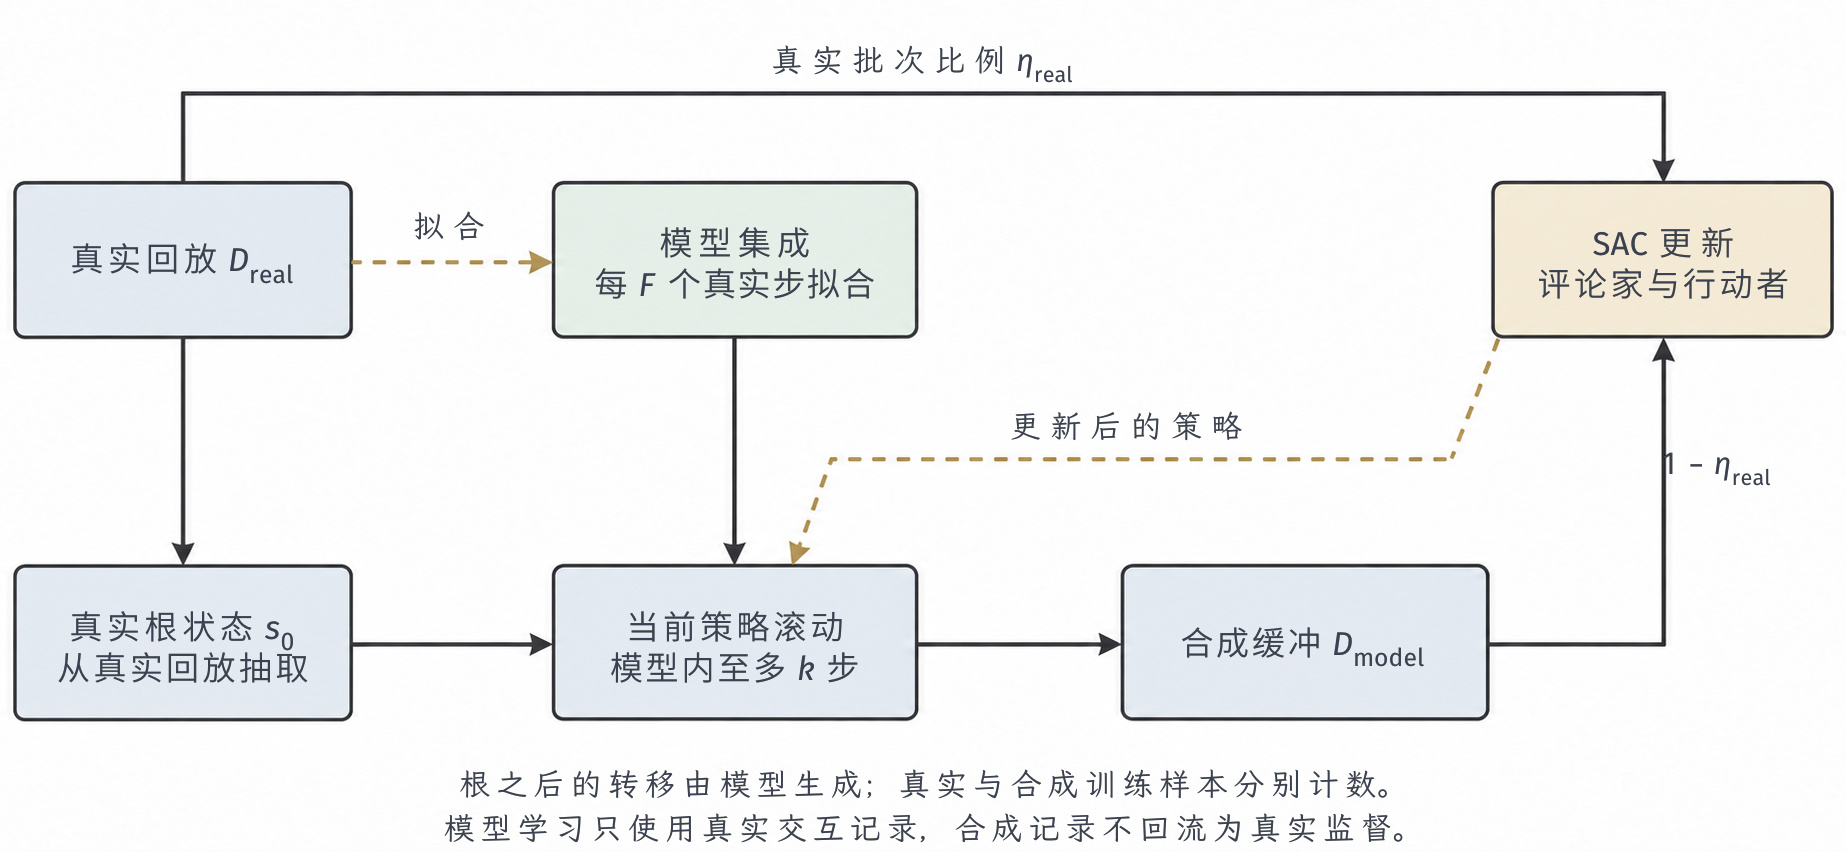
\includegraphics[width=157.400mm]{figures/10-reinforcement-learning/01-problems-and-solving/generated/rl-learning-mbpo/figure.png}
  \caption{MBPO的短分支经验。分支根来自真实回放，根之后的状态、奖励和终止由模型给出；合成缓冲与真实缓冲共同训练SAC。行动者优化时不需要沿动力学反向传播，模型学习仍只以真实交互记录为监督来源。}
  \label{fig:rl-learning-mbpo}
\end{figure*}

一次合成转移可追溯为：从真实记录抽$s=(3,1)$，当前行动者抽到向上，某个集成成员抽到后继$(3,2)$并预测奖励$-0.04$、非终止，于是按$(s,a,r,s',c)$格式把
$((3,1),\text{上},-0.04,(3,2),1)$及模型版本写入模型缓冲，其中$c=1$表示继续。送入采用真实终止字段$z$的SAC回放接口时，须转换为$z=1-c=0$，不能将第五项原样搬入。这一转移在基准网格中可能发生，但本次并没有真的执行；其采样概率取决于所选模型。设后继的SAC目标软值为$0.5$，则这条经验给出的评论家目标仍是$-0.04+0.9\times0.5=0.41$。随后行动者在混合批次的状态上最小化
$\mathbb E[\alpha\log\pi_{\bm\theta}(a\mid s)-\min_iQ_{\bm w_i}(s,a)]$。
这一更新不能因为根是真实状态，就把后继也当成真实观测。

缩短滚动直接减少连续使用错误转移的次数，但也更依赖末端价值。为了量化这项取舍，我们先比较同一起点分布、同一固定策略在真实与学习模型中的$k$步自举评分。设两种分支从$\nu$出发，深度$j$的真实状态动作分布为$q_j^\pi$；以总变差度量后继分布误差，以绝对值度量奖励均值误差，记
\[
 e_T(s,a)=\operatorname{TV}(T(\cdot\mid s,a),\widehat T(\cdot\mid s,a)),
 \qquad e_R(s,a)=|R(s,a)-\widehat R(s,a)|.
\]
假设每个$j<k$都有
$\mathbb E_{q_j^\pi}e_T\leq\epsilon_m$、
$\mathbb E_{q_j^\pi}e_R\leq\epsilon_r$，
两模型奖励均值绝对值不超过$R_{\max}$，并用同一个末端函数$V$且
$\|V\|_\infty\leq V_{\max}$。逐步使用概率核的非扩张性，得到深度$j$的两种状态分布的总变差不超过$j\epsilon_m$。于是两个$k$步自举评分相差至多
\begin{equation}
 B_k=
   \sum_{j=0}^{k-1}\gamma^j
       (\epsilon_r+2R_{\max}j\epsilon_m)
       +2\gamma^kV_{\max}k\epsilon_m.
 \label{eq:rl-learning-short-model-bound}
\end{equation}
奖励误差被分为真实访问处的模型误差与两个访问分布的差，后者乘$2R_{\max}$；末端项同理。若还要与真实无限回报比较，且
$\|V-V^\pi\|_\infty\leq\epsilon_V$，须再加
$\gamma^k\epsilon_V$。短时域降低转移误差累积，却让末端价值误差衰减得更少，不能据此推出$k$越小永远越好。

这个界使用的是目标策略在各深度真实访问处的平均误差，用于评价模型预测误差的转移样本却通常由行为策略$\beta$采集。从$q_j^\beta$转换到$q_j^\pi$，需要知道新策略是否过度访问旧策略轨迹记录很少覆盖的区域。若有
$q_j^\pi(s,a)\leq C_jq_j^\beta(s,a)$，则非负模型误差的期望至多放大$C_j$倍；只知道行为分布上的小均方误差，并不等于已知$\epsilon_m$，更不等于已控制$C_j$。另一种思路是限制
$\sup_s\operatorname{TV}(\pi(\cdot\mid s),\beta(\cdot\mid s))\leq\epsilon_\pi$：
从相同根分布出发，逐步耦合给出策略引起的轨迹分布偏离至多随深度线性增长。MBPO的原始分析正是把训练记录采集策略下的模型总变差误差与策略变化结合，讨论短分支的改进下界；它的抽象单调改进条件不等于实际集成网络加SAC必然单调改进\scite{rl3-janner2019mbpo}

式\eqref{eq:rl-learning-short-model-bound}中的两类转移误差可以按深度理解。第$j$步以前若已有小概率偏离，两种模型就会在不同状态上评分，即使此步各自预测得很准，也可能给不同奖励；这产生$j\epsilon_m$项。末端价值同样受起点之后的偏离影响。把滚动缩短会减少这些项，却让更多未展开回报依赖评论家，这才是短模型滚动的取舍。

若式\eqref{eq:rl-learning-short-model-bound}对整个候选策略集合同时成立，且模型内选择的策略对相应真实目标使用了误差受控的末端值，那么模型代理提升超过两侧总误差才支持真实提升。仅对更新前策略成立的平均验证误差不足以做此推断。表\ref{tab:rl-learning-rollout-controls}列出常用限制各自约束了什么。

\begin{table*}[t]
  \centering
  \small
  \begin{tabularx}{\linewidth}{>{\raggedright\arraybackslash}p{25mm} >{\raggedright\arraybackslash}X >{\raggedright\arraybackslash}X}
    \toprule
    设计 & 直接作用 & 仍未保证的条件 \\
    \midrule
    从真实回放分支 & 避免从模型生成的长历史起步 & 根可能来自旧策略；根之后仍会偏离真实覆盖 \\
    限制$k$并调整日程 & 减少连续使用错误转移的次数 & 不证明末端价值准确，也不证明给定长度最优 \\
    提高真实批次比例 & 减少当前更新中合成转移记录的权重 & 不能补出真实交互记录未覆盖的动作 \\
    集成分歧筛选 & 排除模型成员明显不一致的转移 & 成员可能共同犯错；分歧不是经校准的TV半径 \\
    限制合成转移记录的保留时间 & 降低旧模型生成经验的占比 & 当前模型仍可能有系统性偏差 \\
    \bottomrule
  \end{tabularx}
  \caption{短模型滚动的控制量与边界。它们是需要验证的算法设计，不是全局性能或安全证明。}
  \label{tab:rl-learning-rollout-controls}
\end{table*}

% Outline: 3.5.4
\subsection{模型误差下的策略优化边界}
\label{sec:rl-learning-model-policy-boundary}

不做部署搜索并不能避免模型利用偏差，模型梯度同样会把行动者引向高估区域。设一个独立的一步连续动作教学任务为$a\in[-1,1]$、真实奖励$R(a)=-a^2$，模型奖励
$\widehat R(a)=-a^2+0.8a$。真实训练记录若只包含执行$a=0$后的奖励反馈，模型在那里误差为0；从确定性策略$a=\theta=0$出发，模型梯度却是$0.8$。它最终把动作推到$0.4$，预测奖励$0.16$，真实奖励$-0.16$，而原策略真实奖励为0。这个例子不涉及长时域误差，已经足以说明“多做模型内策略更新”可能降低真实性能。

上例的旧策略只访问$a=0$，模型评价该策略完全准确；优化却选出了旧策略交互记录从未验证的$a=0.4$。因此，从固定策略评估扩大到模型内选策略时，误差控制也要扩大到候选策略会到达的区域，或由对依据训练记录选出的策略也同时有效的置信集合承担这一要求。第\ref{sec:rl-learning-model-bias}节的统一模拟界可支持选择后的回报结论，单点拟合则不能。图\ref{fig:rl-learning-model-feedback}展示策略改变访问分布后需要补充真实验证的反馈，表\ref{tab:rl-learning-model-policy-errors}列出处置位置与代价。

\begin{figure*}[t]
  \centering
  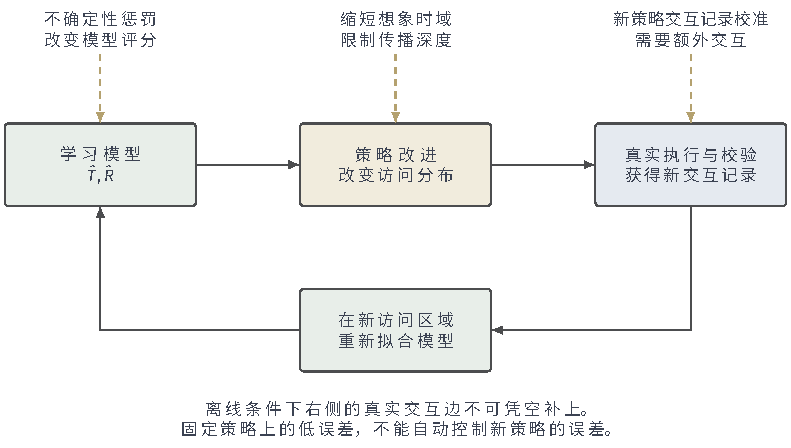
\includegraphics[width=133.960mm]{figures/10-reinforcement-learning/01-problems-and-solving/tikz/rl-learning-model-feedback.pdf}
  \caption{模型策略优化中的访问分布反馈。虚线标明三种限制分别作用的位置；补充真实转移记录要求仍有交互能力，离线训练不能假定这条边随时可用。上例中的模型梯度把策略从已验证的$a=0$推向未验证区域。}
  \label{fig:rl-learning-model-feedback}
\end{figure*}

\begin{table*}[t]
  \centering
  \small
  \begin{tabularx}{\linewidth}{>{\raggedright\arraybackslash}p{26mm} >{\raggedright\arraybackslash}X >{\raggedright\arraybackslash}X}
    \toprule
    误差处置 & 主要限制的环节 & 代价及不足 \\
    \midrule
    不确定性惩罚 & 用$\widehat R-\lambda u$降低未确信区域的代理收益 & 需要$u$对相关错误敏感；可能过度保守、阻碍必要探索 \\
    缩短想象时域 & 减少模型误差传播深度 & 更依赖末端评论家，可能漏掉延迟后果 \\
    真实转移记录校准 & 在新策略访问处验证并更新模型 & 需要额外交互；不可逆损失不能靠事后校准撤销 \\
    限制策略变化 & 避免单次更新过快远离支持区域 & 局部变化小仍可累积成大偏离，旧覆盖不永久有效 \\
    \bottomrule
  \end{tabularx}
  \caption{模型误差措施并不互相替代。惩罚改变评分，短时域改变传播，真实校准增加新策略访问处的转移记录；三者对应不同的误差来源。}
  \label{tab:rl-learning-model-policy-errors}
\end{table*}

动作条件视频模型将预测对象扩大到画面序列，但策略训练仍依赖动作后果是否正确。生成画面可以逼真，却错误地预测“按下这个键便到达门口”。判断其能否支持策略训练，需核对动作接口、视频与动作记录是否覆盖所需干预、奖励和终止的来源、部署能否闭环接收观测，以及真实环境测试结果。开放环视频质量评价观测预测，不能单独继承为闭环回报保证。

\Needspace{20\baselineskip}
Dreamer 4提供了一个具体延伸案例。这里讨论的是2025年9月29日发布的原始预印本版本\scite{rl1-hafner2025-dreamer4}
它使用VPT承包者提供的2541小时、360p、20帧每秒的Minecraft视频及键鼠和事件记录；动作接口包含23个二元按键与121类鼠标动作。模型内学习使用任务嵌入，测试有预设任务提示序列。使用这些视频、动作和事件记录的训练是离线的；即便模型内策略采样是同策略，也不意味着算法在真实环境中在线采集新的训练记录。

该版本报告在1000个随机世界、空背包、每回合60分钟的真实Minecraft测试中，获得钻石的成功率为$0.7\%$。这是闭环环境证据，强于只展示视频，却仍受动作接口、任务提示和视频、动作及事件记录的来源限制；它既不是DreamerV3抽象动作协议下的直接同预算比较，也不是机器人安全保证。模型速度、生成质量和策略成功率应分开报告。

至此，模型的用途已能按真实交互记录、模型预测与更新目标之间的依赖区分：Dyna把模拟转移用于价值备份，MPC与MuZero用模型进行当前决策搜索，Dreamer把想象轨迹用于策略训练，MBPO把短合成转移交给离策略行动者—评论家。一个系统可以同时拥有这些部件；判断其条件，应看真实交互记录如何进入、哪项预测参与了哪次更新，以及最终动作究竟由谁给出。

% Outline: 3.6
\section{时间抽象下的价值与策略学习}
\label{sec:rl-learning-temporal-abstraction}

前述更新默认每步选择一个原子动作。在房间导航中，一段“走到门口”的控制过程可以重复调用，高层不必每步重新选方向。时间抽象（temporal abstraction）把这段持续行为当作一次决策，改变的是决策间隔，而不是是否使用模型或是否优化显式策略。因此它可分别与四种求解组合结合，也仍需要学习内部动作、评价长期回报和取得覆盖相关状态动作的交互记录。

% Outline: 3.6.1
\subsection{时间抽象解决什么问题}
\label{sec:rl-learning-temporal-purpose}

考虑一个完全可观测、突出房间结构的独立确定性教学网格，区别于前文$4\times3$基准：格点为
$x=1,\ldots,8$、$y=1,\ldots,5$；$x=4$与$x=5$之间有墙，仅在$y=2,4$开门。上下左右每步确定移动一格，不合法动作不可选。起点为$(2,2)$、目标为$(7,2)$，入目标奖励1，其余步$-0.04$，$\gamma=0.9$。图\ref{fig:rl-learning-options-rooms}画出原子动作与高层决策的对应。

从起点到目标的最短路线仍需五个原子动作。若预先可调用两步的“到下门左侧$(4,2)$”和三步的“穿下门并到目标”，高层只选择两次，执行层却仍与环境交互五步。时间抽象节省的是高层决策深度：在更大房间中，探索可以保持一段有方向的行为，回报也可评价整个子任务。要取得这些收益，内部控制必须能完成调用，终止规则必须在适当时刻交回控制权；两者本身也有学习代价。

\begin{figure*}[t]
  \centering
  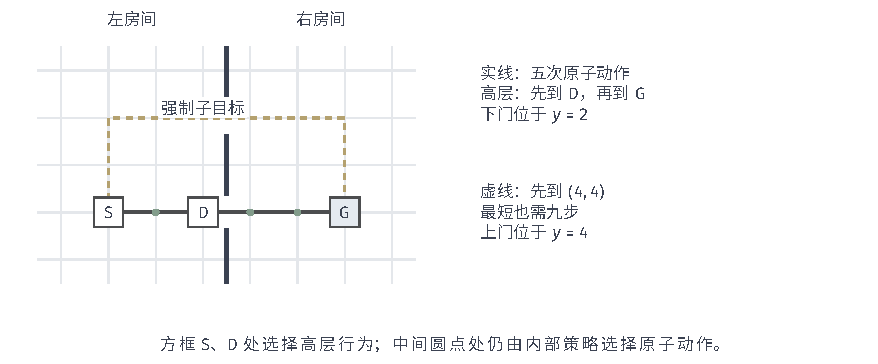
\includegraphics[width=148.749mm]{figures/10-reinforcement-learning/01-problems-and-solving/tikz/rl-learning-options-rooms.pdf}
  \caption{两房间教学网格中的时间抽象。实线路径有五个原子动作，可由两次高层调用组成；虚线路径强制经过上门左侧，多走四步。圆点表示原子时刻，方框标出高层选择时刻。图中几何与奖励规则均为独立教学设定。}
  \label{fig:rl-learning-options-rooms}
\end{figure*}

动作的取值形式与持续时间是两个维度。机器人每毫秒选择一次实数力矩，虽是连续动作，仍是原子决策；“沿墙前进直到门口”可以只有一个离散编号，却持续随机多步。时间抽象本身不改变外在奖励目标，也不承诺内部执行满足安全约束。若为了训练低层另外奖励“接近门口”，还须说明这是辅助目标，以及它是否可能与全局目标冲突。

\begin{table*}[t]
  \centering
  \small
  \begin{tabularx}{\linewidth}{>{\raggedright\arraybackslash}p{24mm} >{\raggedright\arraybackslash}X >{\raggedright\arraybackslash}X}
    \toprule
    职责 & 输入与输出 & 需要指定或学习的对象 \\
    \midrule
    高层选择 & 状态、任务$\to$行为编号或子目标 & 高层策略、每个行为的价值及可启动条件 \\
    内部控制 & 当前状态、行为或子目标$\to$原子动作 & 低层策略，必要时用子任务奖励训练 \\
    终止判定 & 当前状态、行为$\to$是否交还控制 & 终止概率、超时或到达条件；超时不必等于环境终止 \\
    \bottomrule
  \end{tabularx}
  \caption{时间抽象的三个学习对象。手工规则与自动发现是获得这些对象的不同方式，不改变它们各自的职责。}
  \label{tab:rl-learning-hierarchy-objects}
\end{table*}

表\ref{tab:rl-learning-hierarchy-objects}也指出为什么“给动作起一个高层名字”还不够：必须知道在何处可执行、执行期间如何行动、多久返回。只有这些条件明确，才能把一段行为当作新的动作参与备份。

% Outline: 3.6.2
\subsection{半马尔可夫决策与Options}
\label{sec:rl-learning-options}

调用“到门口”后，下一次高层决策可能在两步后，也可能因绕行在更晚发生。高层因此要同时记录终点、期间奖励和持续时间，不能继续把每次调用当成原来的一步动作。半马尔可夫决策保留这三种随机后果；Option则用启动条件、内部动作策略和终止规则描述一个可调用行为。

\begin{example}[持续时间不能忽略]
  \label{ex:rl-learning-option-duration}
  在房间网格的$(4,2)$到$(6,2)$，Option A走两步，Option B先绕行再用四步到同一终点；期间不碰最终目标，奖励均为$-0.04$。假设终点价值为$0.8$，则
  \[
    y_A=-0.04(1+0.9)+0.9^2(0.8)=0.572,
  \]
  \[
    y_B=-0.04(1+0.9+0.9^2+0.9^3)+0.9^4(0.8)=0.38732.
  \]
  若错误地都只折扣一次，目标变为$0.644$与$0.58244$，两者都被高估。持续时间随机时应平均$\gamma^K V(s_{t+K})$，一般不能换成$\gamma^{\mathbb E K}\mathbb E V$。
\end{example}

\begin{definition}[半马尔可夫决策与Markov Option]
  \label{def:rl-learning-option}
  在离散原子时间上，设高层决策时刻为$t_0<t_1<\cdots$，每次持续时间$K_j=t_{j+1}-t_j$为正整数。若给定当前决策状态$s_{t_j}$及所选高层动作后，下一决策状态、期间累计奖励与$K_j$的联合条件律不再依赖更早历史，则称该决策过程为半马尔可夫决策过程。一个Markov Option记为
  $\omega=(I_\omega,\pi_\omega,\beta_\omega)$：
  $I_\omega\subseteq S$是启动集，
  $\pi_\omega(a\mid s)$是内部原子动作策略，
  $\beta_\omega(s)\in[0,1]$是在到达$s$后终止的概率。
  一次调用先执行至少一个原子动作，再根据到达状态检测是否终止；启动条件、内部策略和终止概率只依赖当前状态和Option编号。高层策略$\zeta(\omega\mid s)$只在允许启动的Option中选择。
\end{definition}

“半马尔可夫”保留了决策时刻的状态条件性，但决策间隔不再固定为一步，因此持续时间也进入后果分布。启动集说明在哪些状态能调用，内部策略说明调用期间每步做什么，终止规则说明何时把控制交回高层；缺少其中一项，就不能确定这段行为对应的奖励、终点与时长。这里的$\beta_\omega$专指Option终止概率，与前面行为策略$\beta$的对象不同，下标$\omega$用于区分。

在固定内部策略和终止规则下，起点$s$与Option$\omega$决定终点及持续时间的分布，这正是半马尔可夫模型。原子动作也可保留：令其内部只执行该动作一次并立即终止，即得到持续时间$K=1$的Option。若Option依赖内部记忆或已执行时长，需把所需变量并入状态，不能继续无条件使用上述Markov形式。Options框架将这种多步行为与原有MDP的价值学习连接起来\scite{rl3-sutton1999options}

为了仍评价原任务的折扣回报，我们按一次Option的实际执行边界分组，而不按高层调用次数重新计时。设调用从$t$执行至$t+K$，前$K$步奖励归入本次行为，余下回报从$t+K$开始；逐项写出便有
\begin{align}
 G_t
   &=r_t+\gamma r_{t+1}+\cdots+\gamma^{K-1}r_{t+K-1}
          +\gamma^K(r_{t+K}+\gamma r_{t+K+1}+\cdots)\notag\\
   &=R_t^\omega+\gamma^K G_{t+K},\qquad
 R_t^\omega:=\sum_{j=0}^{K-1}\gamma^j r_{t+j}.
 \label{eq:rl-learning-option-grouping}
\end{align}
这个等式对每次持续时间有限的Option调用成立，再按给定$s_t=s,\omega_t=\omega$的分布取期望，就有
\begin{equation}
 Q^\zeta_\Omega(s,\omega)
  =\mathbb E\left[
       R_t^\omega+\gamma^K
          \sum_{\omega'}\zeta(\omega'\mid s_{t+K})
                       Q^\zeta_\Omega(s_{t+K},\omega')
                    \,\middle|\,s,\omega\right].
 \label{eq:rl-learning-option-bellman}
\end{equation}
因此高层回放至少应保存$(s_t,\omega,R_t^\omega,K,s_{t+K})$与环境终止标志。若终点是环境吸收终止，后继值为0；Option主动结束只是把控制权交回高层，后继值通常不为0。

评价固定高层策略时按$\zeta$平均下一Option；改为控制时，则在下一状态允许启动的$\Omega(s_{t+K})$中取最高估值，以改进后续高层选择。样本更新为
\[
 Q_\Omega(s_t,\omega)\leftarrow Q_\Omega(s_t,\omega)+
  \alpha\left[R_t^\omega+
        \gamma^K\max_{\omega'\in\Omega(s_{t+K})}
                          Q_\Omega(s_{t+K},\omega')
                     -Q_\Omega(s_t,\omega)\right].
\]
把$\gamma^K$写成$\gamma$相当于用高层调用次数重新定义时间，会改变原始任务，而不是同一个目标下的近似实现。

\begin{theorem}[Option备份的压缩性]
  \label{thm:rl-learning-option-contraction}
  设$S$有限，每个非终止状态的可启动Option集$\Omega(s)$有限且非空，原子奖励有界，$0\leq\gamma<1$。固定各Option的内部策略和终止规则，每次调用的持续时间$K\geq1$且几乎处处有限。设$\zeta(\cdot\mid s)$是在$\Omega(s)$上归一的合法平稳高层策略。对有界状态价值函数$V$，定义
  \[
    \begin{aligned}
    (\mathcal B_\Omega^\zeta V)(s)
       &=\sum_{\omega\in\Omega(s)}\zeta(\omega\mid s)
          \mathbb E[R_t^\omega+\gamma^K V(s_{t+K})\mid s,\omega],\\
    (\mathcal B_\Omega^*V)(s)
       &=\max_{\omega\in\Omega(s)}
          \mathbb E[R_t^\omega+\gamma^K V(s_{t+K})\mid s,\omega].
    \end{aligned}
  \]
  两算子在终止状态都定义为0，调用结束于终止状态时的后继价值也取0。对任意有界$V,W$及$\mathcal B\in\{\mathcal B_\Omega^\zeta,\mathcal B_\Omega^*\}$，有
  $\|\mathcal BV-\mathcal BW\|_\infty\leq\gamma\|V-W\|_\infty$。
\end{theorem}

\begin{proof}
  固定$s,\omega$，累计奖励在两次备份相减时抵消，余项绝对值至多为
  \[
    \mathbb E[\gamma^K|V(s_{t+K})-W(s_{t+K})|\mid s,\omega]
      \leq\mathbb E[\gamma^K\mid s,\omega]\|V-W\|_\infty
      \leq\gamma\|V-W\|_\infty.
  \]
  高层概率平均不增大此界；最大值满足
  $|\max_\omega x_\omega-\max_\omega y_\omega|
       \leq\max_\omega|x_\omega-y_\omega|$，故同样成立。对$s$取上确界即得结论。
\end{proof}

固定内部策略和终止规则后，备份误差只来自终点价值，因而实际持续时间越长，这一误差的折扣越强；压缩因子可以收紧为$\sup_{s,\omega}\mathbb E[\gamma^K\mid s,\omega]$。这里取上确界是要覆盖每个可启动状态与Option，并不说明获得长行为的训练样本更少。若Option可能永不终止，原始折扣回报仍可能有定义，但下一高层决策时刻不再总是有限；需要另行规定该事件上的回报与备份，不能直接使用上述陈述。在有界状态价值函数的一致范数空间中，空间完备，且有界奖励使这两个备份仍输出有界函数。它们因此各有唯一不动点，反复应用同一备份会按压缩率收敛；这个结论只用于固定Option集合及内部规则的价值求解。

% Outline: 3.6.3
\subsection{分层价值与策略学习}
\label{sec:rl-learning-hierarchical-learning}

Option备份暂时固定了内部策略和终止规则，接下来要决定怎样获得它们。手工指定“到下门”时，低层读取当前格点和门位置，输出方向，并可用到门奖励训练；高层读取当前房间和外在任务，选择子目标，仍以原始折扣奖励评价。如果不预先指定门位置，Option-Critic可以直接用外在回报训练内部策略及终止概率。图\ref{fig:rl-learning-hierarchy}区分各层输入、动作与奖励，避免把低层辅助目标混成全局任务。

\begin{figure*}[t]
  \centering
  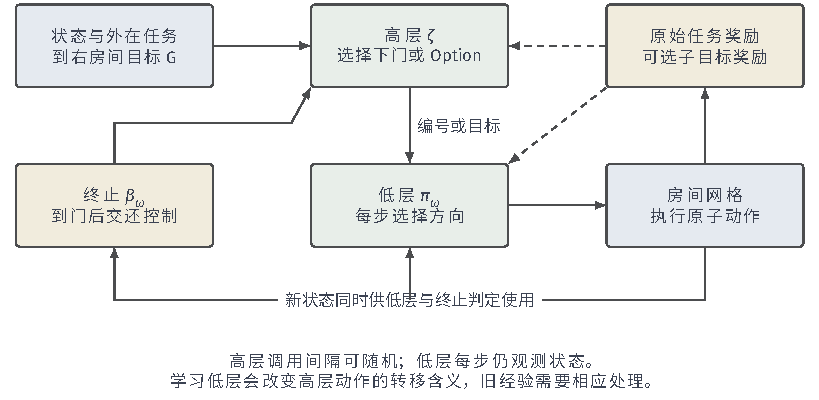
\includegraphics[width=138.747mm]{figures/10-reinforcement-learning/01-problems-and-solving/tikz/rl-learning-hierarchy.pdf}
  \caption{房间任务的分层接口。高层交付子目标或Option编号，低层持续输出原子动作，终止后才交回控制权。右侧区分原始任务奖励与可选的低层辅助奖励；Option-Critic无需人为指定这一辅助奖励。}
  \label{fig:rl-learning-hierarchy}
\end{figure*}

内部规则若也要学习，高层看见的“同一个Option”会随训练改变。过去两步能到门口的调用，今天可能更快，也可能绕行；旧高层记录中的终点和时长未必仍代表当前低层。因此先建立固定内部规则的备份，再讨论联合学习和旧记录校正，有助于分清压缩性究竟针对哪个固定算子。

每个原子步之后既可能继续当前Option，也可能终止并重选，所以评价还需保留当前Option编号。Option-Critic为这两种后续选择分别估值。假定所有Option在所有非终止状态均可启动，记$Q_\Omega(s,\omega)$为当前继续执行$\omega$的价值，
$V_\Omega(s)=\sum_{\omega'}\zeta(\omega'\mid s)Q_\Omega(s,\omega')$为重新选择的价值。到达$s'$后，尚未作终止选择的价值是
\begin{align}
 U(\omega,s')
   &=(1-\beta_\omega(s'))Q_\Omega(s',\omega)
                               +\beta_\omega(s')V_\Omega(s'),\notag\\
 Q_U(s,\omega,a)
   &=R(s,a)+\gamma\mathbb E_{s'\sim T(\cdot\mid s,a)}U(\omega,s'),\notag\\
 Q_\Omega(s,\omega)&=\sum_a\pi_\omega(a\mid s)Q_U(s,\omega,a).
 \label{eq:rl-learning-option-critic}
\end{align}
这些关系允许每个原子步更新评论家，而不必等Option结束。采样转移的目标是
$y=r_t+\gamma U(\omega_t,s_{t+1})$，环境终止时令$U=0$；内部策略则提高$Q_U$大的动作的概率。

固定高层$\zeta$及终止参数，用$\bm\theta$参数化内部策略。定义当前执行状态与Option的归一化占用
$d_\Omega(s,\omega)=(1-\gamma)\sum_{t\geq0}\gamma^t
\mathbb P(s_t=s,\omega_t=\omega)$。环境终止后以零奖励吸收态和固定虚拟Option延拓，使占用总质量仍为1；该延拓不贡献参数梯度。将普通策略梯度应用于包含Option的扩展过程，可得
\begin{equation}
 \nabla_{\bm\theta}J
   =\frac{1}{1-\gamma}
     \mathbb E_{(s,\omega)\sim d_\Omega,\ a\sim\pi_\omega}
       [\nabla_{\bm\theta}\log\pi_\omega(a\mid s)
                                    Q_U(s,\omega,a)].
 \label{eq:rl-learning-intra-option-gradient}
\end{equation}
基线$Q_\Omega(s,\omega)$与动作无关，可以减去以形成内部优势。推导中的占用仍按原子时间折扣，而不是每切换一次Option才折扣。

终止规则的方向可直接从$U$看出。若$\bm\nu$参数化$\beta$，对终止概率的局部导数是
$V_\Omega(s')-Q_\Omega(s',\omega)=-A_\Omega(s',\omega)$。展开未来各次到达的影响，得到
\begin{equation}
 \nabla_{\bm\nu}J
   =-\sum_{t\geq0}\gamma^{t+1}
       \mathbb E[
          \nabla_{\bm\nu}\beta_{\omega_t}(s_{t+1})
                          A_\Omega(s_{t+1},\omega_t)].
 \label{eq:rl-learning-termination-gradient}
\end{equation}
前面的$\gamma$来自先走一步再决定终止。若将到达分布
$(1-\gamma)\sum_t\gamma^t\mathbb P(s_{t+1},\omega_t)$归一化，上式系数就是$-\gamma/(1-\gamma)$。当前Option比重新选择更好时$A_\Omega>0$，梯度会降低终止概率；较差时则提高。高层策略本身若也需求导，应另计高层选择时刻的贡献，不能藏进这个固定$\zeta$的偏导。完整的策略与终止梯度关系见Option-Critic原论文\scite{rl3-bacon2017optioncritic}

例如人工评价值为$Q_\Omega(s',\omega)=0.6$、
$V_\Omega(s')=0.9$，当前$\beta=\sigma(\nu)=0.25$，则
$U=0.675$。前一步奖励$-0.04$、$\gamma=0.9$时，评论家目标为$0.5675$。终止logit的局部上升方向为
$-\beta(1-\beta)A_\Omega=0.05625$；把它乘对应到达折扣权重后，提高终止概率。这一方向不是“价值低就终止”，而是“继续比切换更差就终止”。

其他分层方法主要改变任务分解与交互记录复用方式，不能简单替换上述三个学习对象。Feudal RL用管理者向下层发指令，由下层完成指令获取局部奖励；状态划分与层级接口提供了强先验，也限制了能表达的行为\scite{rl3-dayan1993feudal}

MAXQ把任务写成子任务图，将“执行子任务本身的价值”与“完成它以后还剩多少价值”分开。若在父任务$i$中选择子任务$a$，完成后用$C_i(s,a)$表示父任务剩余部分，则决策评价具有
$Q_i(s,a)=V_a(s)+C_i(s,a)$的结构，完成项包含子任务持续时间的折扣。它学习的是给定分解下的价值；递归最优只要求每个子任务在固定子层下最优，比原始MDP全局最优弱\scite{rl3-dietterich2000maxq}

HIRO用高层给出的相对目标$\bm g_t$训练低层。这里改用连续状态坐标$\bm s_t\in\mathbb R^{d_s}$表示$s_t$，目标也是这组坐标中的位移向量，不通过学习编码重新定义目标距离。高层每$c$个原子步提出一次目标，$c$为固定正整数；窗口内低层以状态与相对目标为输入，并用负距离$-\lVert\bm s_i+\bm g_i-\bm s_{i+1}\rVert_2$作为辅助奖励。令$\bm g_{i+1}=\bm s_i+\bm g_i-\bm s_{i+1}$，便使绝对目的地$\bm s_i+\bm g_i$在窗口内不变。

低层更新会使旧高层动作失去原意：过去“向东两格”的目标现在可能对应另一串原子动作。重标记时保持已经观察的$\bm s_t,\ldots,\bm s_{t+c}$与$a_t,\ldots,a_{t+c-1}$不变，改变的只是起始目标。原实现从10个候选中搜索：旧目标、实际端点位移$\bm s_{t+c}-\bm s_t$，以及8个以该位移为中心的高斯提议。高层接口规定目标各坐标的上下界；高斯提议的各坐标标准差取对应允许范围的四分之一，并裁剪回该范围。这是有限候选近似，不是对任意目标求精确全局最大值。

对每个候选$\widetilde{\bm g}_t$，逐步相对目标由
$\widetilde{\bm g}_i=\bm s_t+\widetilde{\bm g}_t-\bm s_i$，
$i=t,\ldots,t+c-1$确定。用当前含探索噪声的低层行为密度$\pi_{\mathrm{low}}$计算
$\sum_{i=t}^{t+c-1}\log\pi_{\mathrm{low}}
(a_i\mid s_i,\widetilde{\bm g}_i)$，
选择评分最高的候选重标高层经验。在固定各向同性高斯动作噪声下，这相当于最小化记录动作与当前低层均值动作的平方距离和。它校正的是低层行为变化，不是把未发生的真实轨迹补出来\scite{rl3-nachum2018hiro}

HAC则把实际达到的状态作为事后高层动作，并在各层做目标重标记，以近似“下层已经能完成这个动作”的训练接口；另外安排子目标测试，对当前低层不能完成的提议施加相应惩罚。只使用成功的事后重标记、忽略测试，会让上层把不可达子目标估得过高\scite{rl3-levy2019hac}

\begin{table*}[t]
  \centering
  \small
  \begin{tabularx}{\linewidth}{>{\raggedright\arraybackslash}p{22mm} >{\raggedright\arraybackslash}X >{\raggedright\arraybackslash}X}
    \toprule
    方法 & 预先给定的结构 & 学习对象与交互记录复用难点 \\
    \midrule
    Feudal RL & 管理层级、状态抽象与指令接口 & 各层指令选择和执行策略；局部奖励可能限制全局行为 \\
    MAXQ & 子任务图、终止条件及可能的伪奖励 & 子任务值与完成项；保证依赖任务分解和状态抽象条件 \\
    Option-Critic & Option数量、参数化及启动约定 & 内部策略、终止与高层价值；可能退化为过短或重复Option \\
    HIRO & 目标坐标、执行窗口、距离奖励 & 高低层离策略策略；用当前低层动作似然校正旧目标 \\
    HAC & 各层目标空间、执行预算及测试机制 & 多层目标策略；事后动作、事后目标和子目标测试分工不同 \\
    \bottomrule
  \end{tabularx}
  \caption{分层方法的先验与学习边界。表中层级都需要明确的状态、目标、动作和奖励接口，不是把同一个单层算法重复堆叠即可。}
  \label{tab:rl-learning-hierarchy-methods}
\end{table*}

表\ref{tab:rl-learning-hierarchy-methods}所列先验可能降低学习难度，也可能排除好策略。在图\ref{fig:rl-learning-options-rooms}中，若所有高层策略都被强制先到$(4,4)$，最短路线从五步变为九步。对应回报分别是
$-0.04\sum_{j=0}^{3}0.9^j+0.9^4=0.51854$和
$-0.04\sum_{j=0}^{7}0.9^j+0.9^8\approx0.20265$。
即使每个子任务都学得完美，仍无法恢复被层级排除的下门直达路线。若同时保留全部原子动作且允许高层任意选择，它仍可表示原始最优策略，但搜索和学习未必会及时找到它。

% Outline: 3.6.4
\subsection{技能发现与下游复用}
\label{sec:rl-learning-skill-discovery}

手工指定门口已经利用了下游任务知识。没有外在奖励时，可以先训练一组产生不同可控后果的行为，随后检验它们能否被任务策略调用。先考虑取有限标签的\term{技能变量}$Z\in\{1,\ldots,m_Z\}$。固定起点$s_0$与执行时域或终止规则后，先按先验$p(z\mid s_0)$抽取标签，再从$s_0$执行技能策略$\pi(a\mid s,z)$，由策略与环境共同产生后果$Y$。$Y$可取终点、访问状态或轨迹摘要；上述抽样与执行过程共同规定$(Z,Y)$的联合律。判别器$q_{\bm\psi}(z\mid y,s_0)$从后果反推技能。不同技能若总到同一处便难以区分；若差别仅来自不可控噪声，也难以由技能稳定产生。这里希望学习的是选择行为可以改变的后果。

在房间任务中，可以让技能1趋向左下、技能2趋向左上，再训练判别器从终点判断用了哪个技能。如果两个技能总到同一处，终点不能提供辨认技能标签的证据；如果终点区域互不重叠，观察终点就能识别标签。互信息（mutual information）量化这种平均辨识收益：看到行为后果以后，对所选技能还有多少不确定性，比看到后果以前减少了多少。下面比较的是技能标签与后果的联合分布，不是单独追求后果越随机越好。

固定起点$s_0$和执行时域或终止规则。对每个技能$z$，令$Q_z(\mathrm dy\mid s_0)$为执行策略$\pi_z$后、由环境转移及所选轨迹摘要共同生成的后果分布；假设后果空间为标准Borel空间。先验满足$p(z\mid s_0)>0$且$\sum_zp(z\mid s_0)=1$，因此联合律明确为
\[
 P(Z=z,Y\in B\mid s_0)=p(z\mid s_0)Q_z(B\mid s_0).
\]
用联合律与边缘律乘积的KL比较技能选择与后果的依赖，得到
\[
 \begin{aligned}
 I(Z;Y\mid s_0)
 &=D_{\mathrm{KL}}\!\left(P_{Z,Y\mid s_0}\,\middle\|\,
          P_{Z\mid s_0}\otimes P_{Y\mid s_0}\right)\\
 &=\mathbb E\log\frac{p(Z\mid Y,s_0)}{p(Z\mid s_0)}\\
 &=H(Z\mid s_0)-H(Z\mid Y,s_0).
 \end{aligned}
\]
最后两项只对有限技能标签的先验与后验概率求Shannon熵，均有限；自然对数的单位为nat。因此$0\leq I(Z;Y\mid s_0)\leq\log m_Z$，其含义是观察后果平均减少了多少技能不确定性。$Y$可以离散、连续或混合，不能改用$Y$的两个可能无限的熵相减。连续技能等一般变量仍使用联合律的KL表达，互信息可能为无穷，熵差须另查有限性。

赋能（empowerment）用信道容量表达可区分的控制选择。例如，设原子动作集有限且在所有相关状态可用，固定执行长度$K\geq1$；预先选定一个开环动作序列，由环境生成末端状态$S_K$。对允许的序列分布优化，容量为
\[
 \max_{p(a_{0:K-1}\mid s_0)}
       I(A_{0:K-1};S_K\mid s_0).
\]
候选分布仅给合法可执行的序列分配质量。用根据途中观测调整动作的闭环技能替代开环序列，会改变允许的控制类；有限技能目标与这种容量不能直接视为同一个优化问题。

\begin{example}[后果随机，技能仍可完全区分]
  \label{ex:rl-learning-finite-skill-mi}
  在一维位置教学任务中，两个技能以各$1/2$的概率被选取。技能1停在位置0，技能2的终点在$[1,2]$上均匀分布。看见终点便能确定执行了哪个技能，所以$H(Z)=\log2$、$H(Z\mid Y)=0$，互信息为$\log2$。技能2的具体落点仍有随机性，但这不妨碍识别技能。此时$Y$同时含有点质量与连续部分，直接套用普通离散熵或微分熵的差并不合适；有限标签$Z$的熵差仍有明确含义。
\end{example}

计算互信息需要技能与后果的联合分布，但真实后验$p(z\mid y,s_0)$通常不能直接计算。以下仍以有限标签说明，并假设判别器给真实技能的概率为正、有关对数项可积。判别器给出一个可由带技能标签的交互记录拟合的替代概率；用它构造下界，策略就有可计算的训练信号。在互信息的对数比中加减$\log q_{\bm\psi}$，有
\begin{align}
 I(Z;Y\mid s_0)
   &=\mathbb E\left[\log q_{\bm\psi}(Z\mid Y,s_0)
                                  -\log p(Z\mid s_0)\right]\notag\\
   &\quad+\mathbb E_Y D_{\mathrm{KL}}
       (p(\cdot\mid Y,s_0)\|q_{\bm\psi}(\cdot\mid Y,s_0))\notag\\
   &\geq\mathbb E\left[\log q_{\bm\psi}(Z\mid Y,s_0)
                                  -\log p(Z\mid s_0)\right].
 \label{eq:rl-learning-skill-mi}
\end{align}
判别器用带已知技能标签的经验做最大似然训练；策略把括号内的量当作内部奖励。这一推导只用KL非负性，但所得到的学习质量仍取决于后果选择、判别器容量、采样覆盖与优化。固定均匀先验时$-\log p(z)$是常数，不代表每个技能已经覆盖到有用区域。

判别奖励也可以手算。两个技能先验均为$1/2$，若某终点使判别器给真实技能的概率为$0.9$，内部奖励为$\log(0.9/0.5)=\log1.8\approx0.588$；若只能给$0.5$，奖励为0。策略因此被鼓励产生较易辨认的后果，判别器则用已知标签提高分类概率。两者互相影响，并不说明这个后果已经有助于送达右房间的任务目标。

VIC以给定初始状态后的终止状态区分Option，正适合上述条件互信息。终点奖励可经策略梯度分配给整段内部动作，终止规则也是技能含义的一部分\scite{rl3-gregor2017vic}

DIAYN用访问到的状态区分技能，并加入动作熵来鼓励每个技能内的随机性。其常见内部奖励为
$\log q_{\bm\psi}(z\mid s)-\log p(z)$，再由最大熵强化学习优化。它不是VIC的同一个条件终点目标：是否给判别器起点、对哪些时刻的状态取平均，都改变要区分的对象\scite{rl3-eysenbach2019diayn}

DADS希望技能的动力学后果既可预测又不同，目标围绕$I(Z;S'\mid S)$。技能条件动力学$q_{\bm\psi}(s'\mid s,z)$给出形如
\[
 r^{\mathrm{int}}
   =\log q_{\bm\psi}(s'\mid s,z)
    -\log\left[\frac{1}{M}\sum_{m=1}^{M}
                      q_{\bm\psi}(s'\mid s,z_m)\right],
       \qquad z_m\sim p(z)
\]
的近似训练信号：给定技能要能预测后继，不给技能时却有多种可能。有限$M$、学到的动力学和依交互训练记录而定的技能分布都会影响估计，不能把这个有限样本比值一概当成精确互信息。学到的技能动力学还能支持下游在技能空间规划\scite{rl3-sharma2020dads}

\Needspace{20\baselineskip}
CIC则用状态转移与连续技能的对比学习构造行为表示，并在该表示中估计熵来提供探索奖励\scite{rl3-laskin2022cic}
以同一批记录的转移嵌入$\bm v_i$与技能嵌入$\bm u_i$为例，对非零嵌入采用余弦相似度
$\operatorname{sim}(\bm v,\bm u)=
\bm v^\top\bm u/(\lVert\bm v\rVert_2\lVert\bm u\rVert_2)$。
正温度$\tau>0$控制评分差在指数中的放大程度：温度越小，同样的相似度差产生越悬殊的匹配权重。固定技能$\bm u_i$作查询，将同批全部转移嵌入$\bm v_j$作为候选；其中$j=i$是与该技能共同记录的正匹配，其他$j$是批内负样本。按原论文的批内交叉熵形式，匹配损失为
$-\log[\exp(\operatorname{sim}(\bm v_i,\bm u_i)/\tau)/
\sum_j\exp(\operatorname{sim}(\bm v_j,\bm u_i)/\tau)]$。
分母包含正匹配，指数权重归一化后给出它在批内被识别的概率，最小化负对数提高这一相对概率。实际内在奖励还使用表示空间近邻距离的粒子熵估计，不能把这一对比损失直接等同于DIAYN的状态分类奖励。比较这类方法时，应分别检查表示训练与策略奖励的实现。

\begin{table*}[t]
  \centering
  \small
  \begin{tabularx}{\linewidth}{>{\raggedright\arraybackslash}p{19mm} >{\raggedright\arraybackslash}X >{\raggedright\arraybackslash}X}
    \toprule
    方法 & 主要区分对象 & 学习信号和容易遗漏的条件 \\
    \midrule
    VIC & 给定起点后的技能与终点 & 条件判别式下界；终止与可达性决定后果空间 \\
    DIAYN & 技能与技能下访问的状态 & 状态判别奖励加动作熵；可区分状态未必是任务相关状态 \\
    DADS & 给定状态后的技能与后继 & 技能动力学的似然比；预测性和后继多样性同时重要 \\
    CIC & 连续技能与状态转移表示 & 对比表示学习与表示熵奖励；嵌入距离及负样本设计影响结果 \\
    \bottomrule
  \end{tabularx}
  \caption{技能发现并不共享一个通用互信息损失。改变后果变量或条件变量，就改变了“行为不同”的含义。}
  \label{tab:rl-learning-skill-objectives}
\end{table*}

表\ref{tab:rl-learning-skill-objectives}中的多样性都不能单独证明任务可解。图\ref{fig:rl-learning-skill-regions}给出一个反例：三个技能分别到左房间内三个不同区域，终点可完全区分，故均匀技能的终点互信息可达到$\log3$；但所有技能都不会穿门，任意高层组合也到不了右房间目标。这里为说明达到互信息上限，技能内部均确定，且每次调用都只在左房间活动；访问区域是人工定义，不是实测热图。

\begin{figure}[t]
  \centering
  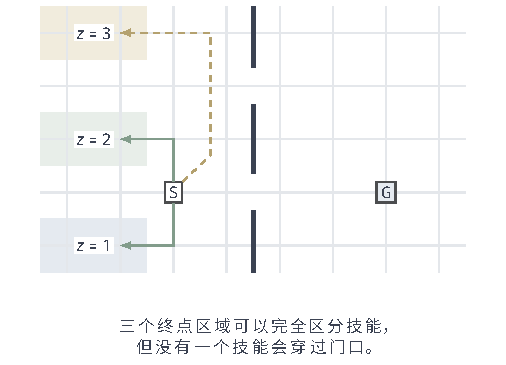
\includegraphics[width=85.750mm]{figures/10-reinforcement-learning/01-problems-and-solving/tikz/rl-learning-skill-regions.pdf}
  \caption{多样但不能完成跨房间任务的技能集合。三种填充和文字标识表示三组不同终点，所有内部策略都限制在墙左侧。可区分性并未提供穿门技能，也未保证一个技能的终点落入另一个有用技能的启动集。}
  \label{fig:rl-learning-skill-regions}
\end{figure}

即使已经有穿门技能，组合还需要启动集相容、终点分布合适和终止时机可靠。评价复用不能只看无奖励阶段相应技能标签与后果之间的互信息或访问区域覆盖面积，还要计入下游技能选择、微调和新增交互成本。这些跨任务问题在第\ref{chap:rl-transfer}章继续展开；时间抽象能改变搜索和学习的单位，但没有取消覆盖、估计与优化三方面的条件。

% Outline: 3.7
\section{样本复杂度与可学习边界}
\label{sec:rl-learning-statistical-limits}

前面给出了经验如何进入更新，也列出了渐近收敛条件。有限预算还需要回答另一个问题：在声明的环境族中，多少真实反馈足以保证输出策略近优，或控制学习期间的回报损失？达到指定策略保证所需的转移样本量，取决于访问协议、问题族和候选函数类。重复梯度与模型生成经验只重复利用已有证据，不能增加这些保证所计数的真实样本。

% Outline: 3.7.1
\subsection{保证对象与数据访问模型}
\label{sec:rl-learning-guarantees-access}

若目标是在训练后得到可部署策略，就应控制输出的次优度，而非仅控制某次训练误差。设算法用$N$次环境反馈输出$\widehat\pi_N$，参照$\pi^*$是在声明策略类中最大化$J$的策略。给定可接受损失$\epsilon$与失败概率$\delta$，大概近似正确（probably approximately correct, PAC）目标把两种要求分开：近似要求回报差不超过$\epsilon$，大概正确要求训练成功概率至少为$1-\delta$。折扣PAC目标要求训练随机性以至少$1-\delta$的概率产生损失不超过$\epsilon$的输出：
\begin{equation}
 \mathbb P\{J(\pi^*)-J(\widehat\pi_N)\leq\epsilon\}
                       \geq1-\delta.
 \label{eq:rl-learning-pac}
\end{equation}
概率覆盖训练记录及算法随机性；$J$本身已经对部署环境取期望。若限制参照为某函数类诱导的策略，就只能称为该类内的近似最优，不应写成全局最优。允许输出一个在回合开始随机选择成员的策略混合时，还应明确这个随机化接口，而不是默认为单个最后网络。

例如$\epsilon=0.1,\delta=0.05$表示：若反复重新采样并训练，至少$95\%$的训练结果应具有不超过$0.1$的期望回报损失。它不要求每条部署轨迹都只损失$0.1$；即使输出策略满足保证，某次滑移仍可能产生很差的实际回报。训练成功事件的概率与固定策略运行后的回报随机性处于两层，下面的遗憾又评价学习期间的全部决策。

有限时域设有$K$回合，每回合$H$步，$T=KH$。记算法第$k$回合使用策略$\pi^{(k)}$，其起点为$s_0^{(k)}$，常见累积伪遗憾为
\begin{equation}
 \operatorname{Reg}_K
   =\sum_{k=1}^{K}\left[
       V_0^*(s_0^{(k)})-V_0^{\pi^{(k)}}(s_0^{(k)})\right].
 \label{eq:rl-learning-episodic-regret}
\end{equation}
每项是给定本回合决策规则后的期望价值差，不是最优期望减去某条实际轨迹的偶然回报。前者关注整个学习过程付出的代价；式\eqref{eq:rl-learning-pac}只关注最终输出。表\ref{tab:rl-learning-guarantee-objects}把容易混淆的量分开。

\begin{table*}[t]
  \centering
  \small
  \begin{tabularx}{\linewidth}{>{\raggedright\arraybackslash}p{24mm} >{\raggedright\arraybackslash}X >{\raggedright\arraybackslash}X}
    \toprule
    保证对象 & 数学陈述或测量量 & 必须说明的输出条件 \\
    \midrule
    PAC输出 & 概率至少$1-\delta$时次优度不超过$\epsilon$ & 固定预算或停止规则；参照类；单策略还是混合策略 \\
    累积遗憾 & $\operatorname{Reg}_K\leq B(K,\delta)$，或其期望界 & 交互过程中全部回合；高概率与期望界不可互换 \\
    Simple regret & 输出次优度$\Delta_N=J^*-J(\widehat\pi_N)$ & 可报告$\mathbb E\Delta_N$或高概率界，须区分二者 \\
    策略识别 & $\mathbb P(\widehat\pi\in\Pi^*)\geq1-\delta$ & 精确识别通常依赖正间隙；等价最优策略可能不唯一 \\
    最后迭代 & 对$\pi^{(K)}$本身保证次优度 & 平均遗憾小不排除最后一轮很差，不能用混合输出替代 \\
    \bottomrule
  \end{tabularx}
  \caption{有限交互样本保证的对象。渐近收敛、PAC输出、学习过程遗憾与最后迭代性质回答不同问题。}
  \label{tab:rl-learning-guarantee-objects}
\end{table*}

例如在固定初始分布下，若平均伪遗憾不超过$\epsilon$，均匀抽取一个已执行策略作为输出，其条件期望次优度不超过$\epsilon$；这还不是概率$1-\delta$的PAC结论。要得到高概率选择，可增加独立评价与置信控制，或使用专门的在线到批量转换。平均策略参数也不等于随机选择策略的混合，神经网络尤其如此。

同一个输出保证，在不同访问能力下可能需要不同样本数。理论中的\term{生成模型}（generative model）是查询预言机：可指定任意合法$(s,a)$，得到独立的真实后继和奖励样本；它不是用有限交互记录训练出的预测模型。基准网格中，这个预言机可直接采样$(4,2)$向上的后果，在线智能体却必须从$(1,1)$先到达那里，还可能滑移。表\ref{tab:rl-learning-access-models}区分查询和实际到达的代价。

\begin{table*}[t]
  \centering
  \small
  \begin{tabularx}{\linewidth}{>{\raggedright\arraybackslash}p{25mm} >{\raggedright\arraybackslash}X >{\raggedright\arraybackslash}X}
    \toprule
    访问协议 & 允许的查询 & 样本保证必须承担的困难 \\
    \midrule
    生成模型 & 指定任意状态动作，抽真实独立转移 & 仍要估计小差异，但免去实际到达目标状态的代价 \\
    在线回合 & 每回合从约定分布或对手给定起点开始 & 必须通过动作取得覆盖，回合内不能任意跳到未见状态 \\
    单条持续轨迹 & 不任意重置，后续状态承接前一动作 & 可达性、返回时间和陷阱；平均奖励常需通信性等条件 \\
    低适应轮数 & 每轮批量采样规则先确定，轮间才能按新取得的转移与奖励记录调整 & 即使总样本相同，反馈轮数有限也可能增加探索成本 \\
    \bottomrule
  \end{tabularx}
  \caption{样本数只有放在访问协议中才有意义。低适应轮数是对查询反馈节奏的附加约束，可以叠加到回合或生成模型协议上。}
  \label{tab:rl-learning-access-models}
\end{table*}

“样本高效”至少应补成一条可检验的任务说明。例如，折扣版本可以是：有限$n_S=|S|,n_A=|\mathsf A|$、奖励在$[0,1]$、$\gamma=0.9$、有生成模型，以概率$0.95$输出满足$J^*-J\leq0.1$的策略，并报告总查询数。有限时域版本应改为$H=20$、$V_H=0$、在线回合采样，以及有限时域价值差；它的回报上界为20，而不是$1/(1-\gamma)=10$。平均奖励版本则需给出持续轨迹、通信MDP及例如直径$D_{\mathrm{diam}}$的条件，以长期增益$g^\pi$或$Tg^*-\sum_{t<T}r_t$为目标，不能沿用折扣$J$。

这些数字只是协议填写示例，不是某算法已达到的实验结果。后文为比较理论将分别声明奖励范围；这也不改变基准网格原有的负步成本。若论文用$K$表示回合数而另一篇用$T$表示时间步，须先代入$T=KH$。同样，按每步奖励不超过1和按整回合总奖励不超过1推导的界，会有不同的时域依赖。

\paragraph{奖励后给定的两阶段探索}
\label{sec:rl-learning-reward-free}
预先围绕一个奖励探索，可能不够支持之后的另一个任务。设机器人先勘查两条通道，再由用户指定配送区域。勘查时没有任务奖励，不能按当前已知高回报路线集中采样；需要先取得能比较未来任务动作后果的转移记录。这就是奖励无关探索要分开的两项工作：先决定访问哪里，再在给定任务奖励后决定怎样行动。

固定非空有限状态集$S$、共同非空有限动作集$\mathsf A$、整数时域$H\geq1$、初始分布$\mu_0$和未知转移核$T_t$，$0\leq t<H$。探索只能按回合从$\mu_0$启动并沿真实状态转移，不能任意跳到待查状态；它观察完整状态，但不使用任务奖励。采集结束后保留有限转移轨迹记录组
$D=(Z_1,\ldots,Z_n)$，其中
$Z_i=(s_{i,0},a_{i,0},\ldots,a_{i,H-1},s_{i,H})$。
规划阶段给出完整的确定性奖励函数组
$R=(R_0,\ldots,R_{H-1})$，每个
$R_t:S\times\mathsf A\to[0,1]$均可计算；允许的全部这类函数组记为$\mathcal R_{\mathrm{task}}$。规划规则只用$D,R$输出$\widehat\pi_{D,R}$，不再采集新的环境轨迹。目标改为有限时域、无折扣回报
$J_H^R(\pi)=\mathbb E_\pi\sum_{t=0}^{H-1}R_t(s_t,a_t)$，
$J_H^{R,*}$是在该任务全部合法策略中的最优值。

奖励可能在看过勘查结果后才确定，所以对某个事先固定奖励的置信保证还不够。给定$\varepsilon,\delta\in(0,1)$，所需的是同一探索事件对所有允许奖励有效：
\begin{equation}
 \mathbb P_{\mathrm{Explore}}\!\left\{
  \sup_{R\in\mathcal R_{\mathrm{task}}}
     [J_H^{R,*}-J_H^R(\widehat\pi_{D,R})]
       \leq\varepsilon\right\}\geq1-\delta.
 \label{eq:rl-learning-reward-free-goal}
\end{equation}
概率针对探索采样及算法随机性；$J_H^R$已经对部署时的状态转移取期望。上确界覆盖全部后给定奖励，而非按某个未声明的奖励分布取平均。一次采集若满足此事件，之后多次更换允许的奖励也无需为这些规划请求再次收集轨迹。

\begin{example}[两条通道与后给定奖励]
 \label{ex:rl-learning-reward-free-branches}
 另设两步确定性教学任务：起点$s_0$选择左或右，第二步任意动作后终止，第一步奖励恒为0。状态集合包含$L,R,B$三个可能后继；两种允许环境中，左动作都到$L$，右动作却分别到$R$和$B$。之后给出的任务甲只在第二步位于$L$时得1，其余为0；任务乙在第二步位于$L,R,B$时分别得$1/2,1,0$。这两套完整奖励函数在两环境中相同，不透露右动作的实际后继。

 若探索只执行左动作，两环境给出相同日志。任务乙中，右到$R$时应选右，右到$B$时应选左，选错都损失$1/2$。即使规划器以概率$q$选择右，两环境的次优差也分别为$(1-q)/2$和$q/2$，至少一个不小于$1/4$。因此同样的左通道日志不能在两环境中都支持误差小于$1/4$的任务乙策略。

 若左右各勘查一次，确定性假设使两个首动作的后果都已确定。任务甲选左得1；任务乙在右通往$R$时选右得1，在右通往$B$时选左得$1/2$，规划时均不用再执行新试验。两条记录足够来自本例的确定性与简单结构；随机通道需要更多样本估计后继概率，不能将这个次数推广为一般保证。
\end{example}

Jin等在有限表格、有限时域设定下构造了满足这种统一保证的探索与规划算法，并给出多项式回合样本上界。其探索先为不同的状态和时刻学习到达策略，再将这些策略组合采样，并在到达后尝试不同动作。用于寻找某状态的指示奖励由探索器自行指定，不是尚未揭示的任务奖励。规划再由记录估计转移，接入给定奖励的近似MDP求解器。覆盖要求按状态在某策略下的最大到达概率调整；对任何策略都极难到达的状态，可将其合计回报影响控制在误差预算内，因此不要求均匀访问全部状态\scite{rl3-jin2020rewardfree}

技能互信息高只说明行为后果可区分，没有给出式\eqref{eq:rl-learning-reward-free-goal}的任务保证；目标重标记也只重算已有转移在另一目标下的奖励。奖励无关探索则把取得足够转移覆盖本身作为前阶段任务，其代价须计入总交互数。这个表格结论不自动扩展到任意潜在表示或神经环境模型。

% Outline: 3.7.2
\subsection{表格MDP的样本复杂度与遗憾}
\label{sec:rl-learning-tabular-complexity}

有限状态动作可以逐对计数，因此探索能直接利用各处尚余的统计不确定性。未充分访问的动作暂留较高估值；真实访问更新经验奖励、转移和置信半径，证据增多后高估值逐渐降低。要让这项不确定性产生远处探索行为，还需通过Bellman备份传回当前可选动作。图\ref{fig:rl-learning-optimistic-grid}将计数与乐观备份并列，说明采样和决策怎样相接。

\begin{figure*}[t]
  \centering
  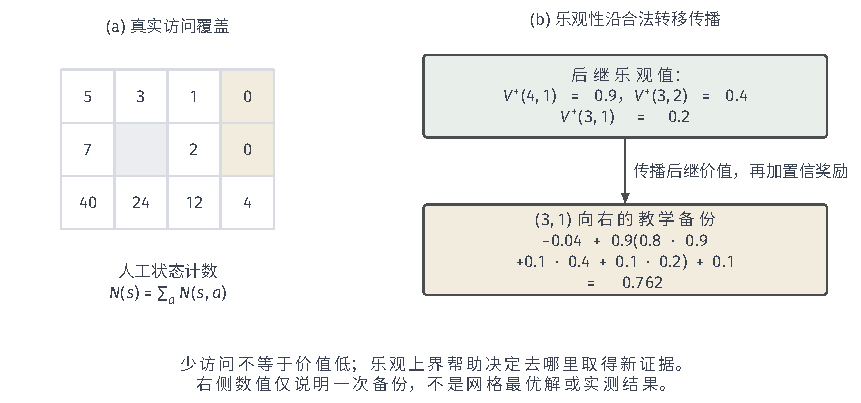
\includegraphics[width=145.750mm]{figures/10-reinforcement-learning/01-problems-and-solving/tikz/rl-learning-optimistic-grid.pdf}
  \caption{计数通过乐观备份影响上游决策。左侧是基准网格合法状态上的人工访问次数，不是实验热图；右侧用一条合法的向右转移说明未知后继的高估值如何影响当前动作。图中折扣教学备份不是下面有限时域UCBVI定理的数值实验。}
  \label{fig:rl-learning-optimistic-grid}
\end{figure*}

E$^3$区分在已知区域利用与主动走向未知区域的策略；R-MAX把不够了解的状态动作暂时接到乐观的高奖励模型\scite{rl3-brafman2002rmax}
两者的重要思想是：无法证明当前策略已经足够好时，就要能以足够概率取得能区分候选环境的新转移或奖励记录。其原始PAC型结果需要声明有限规模、奖励界，以及所用有效时域或混合条件，不能从“模型乐观”直接推出任意持续任务的保证。

回合重置并非每个任务都可用。UCRL2转向持续平均奖励MDP，并要求通信性，即每个状态都能由某种策略到达其他状态。为量化到达代价，定义
$D_{\mathrm{diam}}=\max_{s,s'}\min_\pi\mathbb E_s^\pi\tau_{s'}$
为直径，其中$\tau_{s'}$是到达$s'$的时间。有限$D_{\mathrm{diam}}$排除了某些不可逆陷阱。它在奖励与转移置信集合中选择乐观模型，并按访问计数增长重新规划；在状态与动作集合已知且有限、规模分别为$n_S,n_A$，奖励与转移规律未知、奖励取值位于$[0,1]$的设定下，原论文给出高概率
$\widetilde O(D_{\mathrm{diam}}n_S\sqrt{n_AT})$遗憾界。这个$D_{\mathrm{diam}}$不能用回合长度$H$不加说明地替换\scite{rl3-jaksch2010ucrl2}

\begin{table*}[t]
  \centering
  \small
  \begin{tabularx}{\linewidth}{>{\raggedright\arraybackslash}p{20mm} >{\raggedright\arraybackslash}X >{\raggedright\arraybackslash}X}
    \toprule
    方法 & 保证目标及访问方式 & 乐观机制与必要条件 \\
    \midrule
    E$^3$ & 有限MDP的PAC型学习，原分析包含有效时域与混合条件 & 已知区域评价与到达未知区域的探索规划分开 \\
    R-MAX & 有限MDP近最优学习；平均奖励表述依赖适当混合时间参数 & 不足计数的状态动作给予最大回报的乐观模型 \\
    UCRL2 & 无重置的持续任务遗憾 & 有限直径的通信MDP，奖励和转移置信集合上规划 \\
    UCBVI & 固定长度在线回合的遗憾 & 经验转移与价值置信奖励；下述结果使用时齐转移 \\
    \bottomrule
  \end{tabularx}
  \caption{表格探索保证的任务条件。PAC与遗憾不能只按一个样本数排列，持续任务与回合任务也不具有相同访问能力。}
  \label{tab:rl-learning-tabular-methods}
\end{table*}

理解遗憾界的数量级，可以先看平方根关系。若累积损失主项随$\sqrt T$增长，平均每步损失就随$1/\sqrt T$下降；总试验代价仍在增加，单位时间的代价却逐渐减小。后面用$O$记只关注数量级的上界，$\widetilde O$还省略对数因子；这两种记法都不表示所有预算下实际损失等于主项。显式的次要项和成立条件仍决定有限预算时能用哪个结论。

表\ref{tab:rl-learning-tabular-methods}中的UCBVI直接在经验Bellman备份上加置信奖励。为展示一个具有明确时域依赖的结果，以下固定原论文的设定：$n_S$个状态、每状态$n_A$个动作、已知确定性奖励$R(s,a)\in[0,1]$、未知时齐转移$T$，每回合$H$步，$V_H=0$，没有任意状态查询；回合起点可以由环境选定。第$k$回合前的总访问数为$N^{(k)}(s,a)$，经验转移为$\widehat T^{(k)}$。因为真实$T$不随回合内时刻改变，转移样本可跨时刻合并；若每个时刻有独立$T_t$，统计维数与界会改变。

这一有限时域目标没有折扣，后继价值按剩余步数直接加入。反向计算时，先以经验转移平均后继值，再加置信奖励得到上界；取合法动作的最大值来选择较高回报。还用全程上限$H$和历史上界限制估值，典型更新为
\[
 Q_t^{(k)}(s,a)
   =\min\left\{Q_t^{(k-1)}(s,a),\,H,\,
       R(s,a)+\widehat T^{(k)}V_{t+1}^{(k)}(s,a)
                         +b_t^{(k)}(s,a)\right\},
\]
$V_t^{(k)}=\max_aQ_t^{(k)}$；未访问项保持乐观上限。设共运行$K$回合，真实步数$T=KH$，允许失败概率$\delta\in(0,1)$；以下$L=\log(5Hn_Sn_AT/\delta)$是同时控制各回合、时刻和状态动作的对数参数，不是前面模型滚动的长度。更低的允许失败概率会增大$L$，因而扩大置信半径。简单Hoeffding半径取$H\sqrt{L/N}$量级能说明机制，但不能冒领Bernstein--Freedman（BF）版本的较好界。BF使用后继价值的经验方差，并对随机估值引入额外校正。记$N=N^{(k)}(s,a)>0$、$\widehat T=\widehat T^{(k)}(\cdot\mid s,a)$，
$n_{t+1}^{(k)}(y)$为先前回合在相应时刻访问状态$y$的次数，写出其三个部分：
\begin{align}
 b_t^{(k)}(s,a)
  &=\sqrt{\frac{8L\operatorname{Var}_{\widehat T}
                                  (V_{t+1}^{(k)})}{N}}
       +\frac{14HL}{3N}\notag\\
  &\quad+\sqrt{\frac{8}{N}\sum_y\widehat T(y)
         \min\left\{
           \frac{100^2H^3n_S^2n_AL^2}{n_{t+1}^{(k)}(y)\vee1},H^2
                  \right\}} .
 \label{eq:rl-learning-ucbvi-bonus}
\end{align}
这里数值记号$x\vee1=\max\{x,1\}$，使后继状态计数为0时分母仍至少为1，不表示逻辑“或”。第一项按经验后继价值方差设平方根半径，第二项是有限样本范围修正，第三项补偿估值本身由同批转移记录拟合造成的误差；其中求和按经验后继分布平均，各状态的修正取计数界与$H^2$中较小者。零次计数仍以乐观上限处理，末端已知零价值无需估计。若省去第三项，就不能把由同批转移记录拟合的$V_{t+1}^{(k)}$方差直接当成固定真实价值的方差来使用原保证。

\begin{theorem}[UCBVI-BF的一个有限时域遗憾界]
  \label{thm:rl-learning-ucbvi}
  设状态数$n_S\geq1$、每状态动作数$n_A\geq1$、回合长度$H\geq1$及回合数$K\geq1$均为整数，$T=KH$。奖励为已知确定性函数$R(s,a)\in[0,1]$，未知环境转移核时齐；每回合从环境给定起点在线交互$H$步，终值$V_H=0$，不能任意查询其他状态。取$\delta\in(0,1)$及$L=\log(5Hn_Sn_AT/\delta)$。采用UCBVI-BF原算法，正计数项的置信奖励为式\eqref{eq:rl-learning-ucbvi-bonus}，零计数项保持乐观上限$H$。以至少$1-\delta$的概率，
  \begin{equation}
    \operatorname{Reg}_K
      \leq30L\sqrt{Hn_Sn_AT}
          +2500H^2n_S^2n_AL^2
          +4H\sqrt{TL}.
    \label{eq:rl-learning-ucbvi-bound}
  \end{equation}
  这里的遗憾为式\eqref{eq:rl-learning-episodic-regret}的回合价值差之和。次要项没有被并入主项；只有在相应大样本区域，才适合用
  $\widetilde O(\sqrt{Hn_Sn_AT})$概括其主导尺度。
\end{theorem}

该结果来自Azar、Osband与Munos的定理2；其以回合数表示的首项为$30HL\sqrt{n_Sn_AK}$，末项为$4H^{3/2}\sqrt{KL}$，代入$T=KH$后得到上式。下面解释证明的四个支点，不将简化推导替代原论文对常数和次要项的完整处理\scite{rl3-azar2017ucbvi}

\paragraph{置信事件支持反向乐观性}
加上置信奖励的价值备份首先要成为真实价值的上界，才能指导探索。因此需在奖励已知的设定下，对全部回合、时刻和状态动作同时建立转移集中事件，而不仅保证当前所选动作。由$V_H=0$反向归纳，控制
$(\widehat T-T)V^*_{t+1}$以及同批转移记录拟合的估值带来的额外项，证明
$V_t^{(k)}\geq V_t^*$。对动作取最大保留上界；在多个历史上界中取最小也保留上界，因为它们在同一事件上均不低于真实值。只控制当前访问点，或只控制一个预先固定价值函数，均不足以完成对依赖同批转移记录的估值所作的整段归纳。

\paragraph{把回合损失分成奖励与鞅差}
乐观性使$V_0^{(k)}-V_0^{\pi^{(k)}}$足以覆盖本回合真实遗憾。沿实际访问轨迹展开Bellman关系，后继价值差的条件平均与本次实现之间留下零条件均值的随机项，这就是鞅差；其余由置信奖励和误差修正控制。相邻价值项逐步抵消后，只需累加实际访问处的这些量，不必每回合对全部$n_Sn_A$项重复付出误差。因此，下一步可以利用各处访问次数，而非仅按总时长给粗界。

\paragraph{用访问数而非时间粗界}
对同一状态动作反复访问，平方根半径大致按本地次数$n^{-1/2}$下降。将这一串递减半径求和，再合并全部状态动作的访问预算，关键关系为
\[
  \sum_{n=1}^{m}\frac1{\sqrt n}\leq2\sqrt m,\qquad
  \sum_{n=1}^{m}\frac1n\leq1+\log m,\qquad
  \sum_{s,a}\sqrt{N_T(s,a)}\leq\sqrt{n_Sn_AT}.
\]
前两个界分别控制平方根半径和逆计数修正；最后一步用Cauchy--Schwarz及$\sum_{s,a}N_T(s,a)=T$将各处次数合并。这也说明半径缩小所依据的是新的真实访问，不能用重复训练次数代替没有增加的观测数。

\paragraph{用方差避免多付一个时域因子}
计数求和仍需知道每个半径的尺度。若每步都仅用后继价值范围$H$给界，就忽略了整回合随机性的共同限制，累计时会多付时域因子。BF分析利用沿轨迹的条件方差总和与总回报方差的关系，并用Freedman不等式控制鞅项；随机估值另由式\eqref{eq:rl-learning-ucbvi-bonus}末项校正。将方差累计与访问计数结合，得到$\sqrt{Hn_Sn_AT}$主项，罕见状态和估值修正仍保留为显式次要项。

在相同在线、有限、时齐模型的适当非退化参数及足够大$T$范围内，存在问题族使最坏情形期望遗憾至少为$c\sqrt{Hn_Sn_AT}$量级，$c>0$为通用常数；因此上述主项对$n_S,n_A,H,T$的依赖有相应辨识困难支撑。这是期望下界与高概率上界的尺度比较，不是把两者概率陈述视为相同。若允许每个时刻独立变化的转移核，或者用整回合奖励归一化，必须重新比较，不应引用同一式子。第\ref{sec:rl-learning-statistical-lower}节再用可完整计算的问题对解释下界如何产生。

% Outline: 3.7.3
\subsection{结构化函数逼近的样本效率}
\label{sec:rl-learning-linear-complexity}

图像或连续状态中几乎每次观测都不同，逐状态计数无法等到每处充分访问。跨状态共享样本需要可检验的结构，而不是仅让网络在未见状态动作对上给出较小的预测误差。线性价值近似只规定预测形式；线性MDP进一步要求奖励与转移共同由已知特征线性表示，使各种后继价值的备份也留在同一特征空间。下面区分这种结构与线性混合模型，避免把名称中的“线性”当成相同保证。

仅用线性网络预测价值，约束的是一个函数的形状；让转移具有线性结构，约束的是全部动作后果。一个容易理解的特例是用两个已知非负特征，和为1，混合两份未知后继分布。给定$(s,a)$，特征决定两份分布各占多少；任何后继价值$V$的期望都按同样权重混合，所以换一个$V$仍能用原特征表达。一般线性MDP允许更广的测度表示，但始终要求最终转移是合法概率分布。正是这种对所有后继测试函数都保留的结构，让中间Bellman目标可以共享样本。

\begin{definition}[线性MDP与线性混合MDP]
  \label{def:rl-learning-linear-mdp}
  设$H,d\geq1$为整数，$S$为可测状态空间，合法状态动作域可测。在时刻$t=0,\ldots,H-1$，已知可测特征
  $\bm\phi(s,a)\in\mathbb R^d$，存在未知参数$\bm\theta_t\in\mathbb R^d$和有限有符号测度组成的向量$\bm\mu_t=(\mu_{t,1},\ldots,\mu_{t,d})$使
  \[
    R_t(s,a)=\bm\phi(s,a)^\top\bm\theta_t,\qquad
    T_t(B\mid s,a)=\bm\phi(s,a)^\top\bm\mu_t(B)
  \]
  对每个时刻$t$、每个合法$(s,a)$及每个可测集合$B\subseteq S$成立，则称为相应特征下的线性MDP。奖励均值有限，转移表达必须对各$B$非负且在$B=S$时等于1。
  线性混合MDP的一种常用形式则是已知基核$T_{t,i}$、未知混合权重$\eta_{t,i}$：
  \[
    T_t(\cdot\mid s,a)=\sum_{i=1}^d\eta_{t,i}T_{t,i}(\cdot\mid s,a),
       \qquad \bm\eta_t\in\Delta_d.
  \]
  更一般的线性混合允许其他系数约束，但仍必须保证最终概率核合法。
\end{definition}

第一种结构把状态动作依赖放在已知特征中，未知的是后继状态上的测度；第二种把每个候选后果分布预先给出，未知的是共享系数。在线性混合下，对给定$V$可计算特征
$(T_{t,1}V(s,a),\ldots,T_{t,d}V(s,a))$，它随$V$改变。在线性MDP下，原特征$\bm\phi(s,a)$不随目标改变。二者都称“线性”，并不表示证明条件可以互换。

线性MDP支持价值泛化的原因可直接推导。对任何有界后继价值$V$，
\begin{equation}
 R_t(s,a)+T_tV(s,a)
   =\bm\phi(s,a)^\top
       \left(\bm\theta_t+\int V(s')\,\mathrm d\bm\mu_t(s')\right).
 \label{eq:rl-learning-linear-backup}
\end{equation}
因此每次Bellman备份都仍是相同特征的线性组合。仅有$Q^*$线性可表示，则只约束一个最终解，不能推出任意中间$V$都满足式\eqref{eq:rl-learning-linear-backup}。

这一闭合关系允许用真实转移回归价值参数，而无需枚举后继状态。LSVI-UCB在每回合开始反向重算旧样本的后继目标，做正则化最小二乘，再按未充分约束的特征方向加置信奖励。对第$k$回合，定义先前同一时刻的特征
$\bm\phi_t^{(i)}=\bm\phi(s_t^{(i)},a_t^{(i)})$，令$Q_H^{(k)}=0$，由$t=H-1$向0计算
\begin{align}
 \bm\Lambda_t^{(k)}
   &=\lambda\bm I+\sum_{i<k}
                         \bm\phi_t^{(i)}\bm\phi_t^{(i)\top},\notag\\
 \bm w_t^{(k)}
   &=(\bm\Lambda_t^{(k)})^{-1}
       \sum_{i<k}\bm\phi_t^{(i)}
       \left[r_t^{(i)}
             +\max_aQ_{t+1}^{(k)}(s_{t+1}^{(i)},a)\right],\notag\\
 b_t^{(k)}(s,a)
   &=b_{\mathrm{conf}}\sqrt{\bm\phi(s,a)^\top
                     (\bm\Lambda_t^{(k)})^{-1}\bm\phi(s,a)},\notag\\
 Q_t^{(k)}(s,a)
   &=\min\{H,\bm\phi(s,a)^\top\bm w_t^{(k)}
                                       +b_t^{(k)}(s,a)\}.
 \label{eq:rl-learning-lsvi}
\end{align}
之后执行$a_t^{(k)}\in\argmax_aQ_t^{(k)}(s_t^{(k)},a)$收集一整回合，将真实记录加入下一轮拟合。上式使用原算法的全程上限$H$；当前回合的后继估值会重新生成旧样本的回归目标，不能把它误解成只更新最新一个样本的固定标签回归。

\begin{figure}[t]
  \centering
  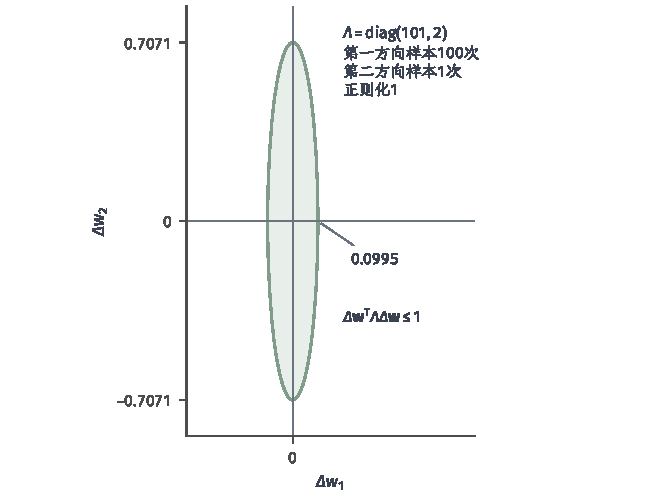
\includegraphics[width=112.000mm]{figures/10-reinforcement-learning/01-problems-and-solving/matplotlib/rl-learning-linear-design.pdf}
  \caption{经验设计矩阵约束的是特征方向。人工例子中$\bm\Lambda=\operatorname{diag}(101,2)$，参数误差椭圆在第一方向很窄、第二方向较宽。即使某个新状态从未出现，只要其特征方向已有充分回归训练样本，置信半径也可能较小。}
  \label{fig:rl-learning-linear-design}
\end{figure}

图\ref{fig:rl-learning-linear-design}中的矩阵来自$\lambda=1$、100个$\bm e_1$样本和一个$\bm e_2$样本。去掉共同系数$b_{\mathrm{conf}}$后，两方向的置信半径分别为
$1/\sqrt{101}\approx0.0995$和$1/\sqrt2\approx0.7071$。半径关心回归训练样本是否约束了该特征方向，而不是网络是否见过该状态动作对。已知特征若没有上述模型实现性，椭圆再窄也可能自信地逼近一个错误模型。

\begin{theorem}[线性MDP中LSVI-UCB的代表性保证]
  \label{thm:rl-learning-lsvi}
  设$d,H,K\geq1$为整数、$\delta\in(0,1)$。考虑可观测状态、有限非空合法动作集、$H$步在线回合，$T=KH$，初始状态允许由环境选择，奖励为确定性$R_t(s,a)\in[0,1]$。真实MDP满足定义\ref{def:rl-learning-linear-mdp}的线性MDP表示，已知
  $\|\bm\phi(s,a)\|_2\leq1$、
  $\|\bm\theta_t\|_2\leq\sqrt d$；为明确测度有界性，取充分条件
  \[
    \left\|\int v(s')\,\mathrm d\bm\mu_t(s')\right\|_2
                          \leq\sqrt d\,\|v\|_\infty
        \quad\text{对所有有界可测 }v.
  \]
  采用$\lambda=1$与充分大的通用常数$c$，令
  $b_{\mathrm{conf}}=c\,dH\sqrt{\log(2dT/\delta)}$。LSVI-UCB以至少$1-\delta$的概率满足
  \[
    \operatorname{Reg}_K
       \leq C\sqrt{d^3H^3T}\log(2dT/\delta)
       =\widetilde O(\sqrt{d^3H^3T}),
  \]
  其中$C$为通用常数。它不需要生成模型访问，也没有显式状态数依赖；动作最大化和特征计算仍必须可执行。
\end{theorem}

这是Jin等人的线性MDP结果；上面将测度规范写成对所有有界测试函数的充分有界条件，避免把有符号测度的总质量与总变差混淆。论文对奖励随机性及模型失配另有讨论，此处不把那些扩展条件省略后并入定理\scite{rl3-jin2020lsvi}

证明沿两条线推进。统计上，式\eqref{eq:rl-learning-linear-backup}使真实备份存在一个范数受控的线性参数；正则化最小二乘的误差可由
$\|\bm\phi\|_{\bm\Lambda^{-1}}$界住。训练转移记录是自适应采集的，后继估值又使用了整批训练记录，因此既要用自归一化鞅集中，也要对算法可能生成的价值类作统一控制，不能把普通独立回归置信区间直接照搬。

决策上，反向归纳得到乐观性，再把遗憾分解为访问轨迹上的置信奖励与鞅项。矩阵行列式引理给
\[
 \det(\bm\Lambda+\bm\phi\bm\phi^\top)
    =\det(\bm\Lambda)(1+\|\bm\phi\|_{\bm\Lambda^{-1}}^2),
\]
所以有限时刻内所有新方向的不确定性总和受$\log\det\bm\Lambda$控制。结合
$\det\bm\Lambda\leq(1+K/d)^d$量级的上界、Cauchy--Schwarz及$H$个时刻的求和，得到累计遗憾界。这是表格访问计数在共享特征空间中的对应物。

该保证约束了整个奖励与转移结构，而不仅是最优值的拟合误差。若任意神经网络在训练样本上能拟合$Q^*$，不能据此认定它具有已知特征、Bellman封闭性、可校准置信半径或高效动作最大化。表示学习可以帮助发现结构，但“能够训练”与“已满足该结构定理”仍是不同判断。

% Outline: 3.7.4
\subsection{一般函数类的可学习条件}
\label{sec:rl-learning-function-classes}

线性MDP的转移结构让中间备份仍可用同一特征表示。一般函数类未必如此：它可能包含最终正确答案，却不能拟合某个候选产生的下一次目标。因此需要分开约束正确答案的可实现性和中间备份的Bellman完备性，而不能只用训练容量回答两者。

先用$\mathcal F_t$记时刻$t$允许选择的价值函数集合，观察“包含答案”与“容纳下一次目标”的差别。

考虑两步、每步一个状态且只有一个动作、奖励全为0的教学任务。取
$\mathcal F_1=\{0,1\}$、$\mathcal F_0=\{0,2\}$，这里集合元素表示常数函数。真实最优值$(Q_0^*,Q_1^*)=(0,0)$在类里；但把候选$f_1=1$备份到前一步得到$\mathcal B_0^*f_1=1\notin\mathcal F_0$。因此可实现不保证每次回归目标可表示。反过来，在该有限时域、固定零终值与相同最优备份算子的完整闭合条件下，可从终点反向推出可实现性；这依赖这些匹配条件，而不是两个术语永远同义。

\begin{definition}[可实现性与Bellman完备性]
  \label{def:rl-learning-realizability}
  设$H\geq1$为整数，$S$为可测状态空间，动作空间$\mathsf A$有限，合法状态动作域可测，各非终止状态的$\mathsf A(s)$非空，终止状态补上零奖励吸收动作，奖励均值可测且有界。有限时域总回报不另加折扣。对$t=0,\ldots,H-1$，$\mathcal F_t$是合法状态动作域上的非空有界可测实函数类，令$\mathcal F_H=\{0\}$及$\mathcal F=\prod_{t=0}^{H-1}\mathcal F_t$。可实现性要求对每个$t$都有$Q_t^*\in\mathcal F_t$。最优Bellman备份定义为
  \[
    (\mathcal B_t^* f_{t+1})(s,a)
       :=R_t(s,a)+\mathbb E_{s'\sim T_t(\cdot\mid s,a)}
                   \max_{a'\in\mathsf A(s')}f_{t+1}(s',a'),
  \]
  其中$t=H-1$的终值项为0。Bellman完备性要求对每个$t$及每个$f_{t+1}\in\mathcal F_{t+1}$，整个备份函数$\mathcal B_t^*f_{t+1}$属于$\mathcal F_t$。若用另一回归类$\mathcal G_t$容纳备份，则相应要求为$\mathcal B_t^*\mathcal F_{t+1}\subseteq\mathcal G_t$，不能省略两个候选类的区别。
\end{definition}

可实现性和完备性仍不直接限制辨识所需样本。庞大候选类若每次观测只排除一个独立候选，就可能需要大量试验；若候选错误共享有限个方向，同一访问分布上的检验可同时约束许多候选。Bellman rank度量探索分布与候选平均Bellman误差之间能否由有限维内积表示，下面正式写出这种分解。

可以把候选检验排成一张表：每一行是一种把智能体带到不同位置的探索策略，每一列是一份待检验价值函数，表项是该候选在这一访问分布下的平均Bellman误差。若表项必须逐个独立检验，所需交互样本数会随表规模增长；若它们能由较少的共同方向表示，一批访问就能约束多个候选。Bellman因子分解把行和列分别映成短向量，再以内积产生表项；分解维数度量这种共享结构，而不是神经网络有多少参数。

\begin{definition}[一种Bellman因子分解]
  \label{def:rl-learning-bellman-rank}
  设$H,M\geq1$为整数、$\zeta\geq0$有限，环境初始分布$\mu_0$和奖励转移核固定，合法动作集有限非空。候选类$\mathcal F$的每个元素为$H$元组$f=(f_0,\ldots,f_{H-1})$，其中各$f_t$为合法状态动作域上的有界可测实函数，约定$f_H\equiv0$；所讨论策略下每步奖励绝对可积。对每个$f\in\mathcal F$和时刻$t$，按固定并列规则选择贪心动作$a_{f,t}(s)$，并令$\pi_f$为它诱导的确定性策略。对$f,g\in\mathcal F$，从$\mu_0$出发，在$t$之前执行$\pi_g$，在$t$及下一步执行$\pi_f$，按环境核生成奖励和后继。定义
  \[
    \operatorname{BE}_t(f,g)=\mathbb E[
       f_t(s_t,a_{f,t}(s_t))-r_t
       -f_{t+1}(s_{t+1},a_{f,t+1}(s_{t+1}))],
  \]
  其中$t=H-1$时最后一项按约定取0，不需在终止后选动作。若对每个$t$都存在映射$\bm\nu_t,\bm\xi_t:\mathcal F\to\mathbb R^M$，使对所有$f,g\in\mathcal F$都有
  \[
    \operatorname{BE}_t(f,g)=\bm\nu_t(g)^\top\bm\xi_t(f),\qquad
    \|\bm\nu_t(g)\|_2\|\bm\xi_t(f)\|_2\leq\zeta,
  \]
  则称该环境与候选类具有维度至多$M$、范数参数$\zeta$的Bellman因子分解。它依赖环境、候选类及生成访问分布的策略，不能理解为网络权重矩阵的秩。
\end{definition}

白话地说，$\bm\nu_t$描述“这次探索把我们带到了哪里”，$\bm\xi_t$描述“这个候选在那里会错多少”，二者通过有限维内积相遇。表格MDP可把状态概率与逐状态误差作为两向量；结构更强时，所需维数可以小于状态数。这种分解不要求算法知道两映射，但证明靠它限制需要多少次有用的排除。

\begin{theorem}[低Bellman rank下的有限类PAC结果]
  \label{thm:rl-learning-olive}
  考虑$H$步在线回合，可从固定初始分布重新开始，动作数为有限$n_A$，每步奖励非负且整回合奖励和几乎处处不超过1。给定有限价值类$\mathcal F$，$|\mathcal F|=N$，函数值在$[0,1]$，终值为0，且真实$Q^*$可实现。假设该类与环境满足定义\ref{def:rl-learning-bellman-rank}的分解，并将范数上界取为$\zeta\geq1$；原上界不足1时可上调为1，不改变分解条件。
  对任意$\epsilon,\delta\in(0,1)$，OLIVE采用原论文阈值与批量样本数，可在
  \[
    \widetilde O\left(
       \frac{M^2H^3n_A}{\epsilon^2}
                         \log\frac{N\zeta}{\delta}\right)
  \]
  个回合内，以至少$1-\delta$的概率输出次优度不超过$\epsilon$的贪心策略。波浪号还隐藏$M,H,n_A,1/\epsilon$的对数项；若按原子环境反馈计数，须再乘$H$。
\end{theorem}

这一陈述是Jiang等人的OLIVE结果在最优值可实现情形下的特例。原框架允许更一般的上下文决策过程及对有效候选类的比较；这里所列特例限定为MDP。其奖励按整回合归一化，不能将该$H$依赖直接与前节每步奖励$[0,1]$的界比较\scite{rl3-jiang2017olive}

OLIVE将这个分解用于候选排除。它在尚未被交互记录否定的函数中选择初始预测回报最高的$f$，再真实执行$\pi_f$检验回报。若预测与实测的差在规定阈值内，且$Q^*$一直未被排除，乐观预测就支持该策略近优；若差距大，则需要找到可检验的错误位置。沿轨迹将候选的相邻价值项抵消，得到
\[
 \mathbb E f_0(s_0,a_{f,0}(s_0))-J_H(\pi_f)
                 =\sum_{t=0}^{H-1}\operatorname{BE}_t(f,f),
\]
其中$J_H$表示该有限时域总回报。故至少一个时刻的Bellman误差足够大。算法按$\pi_f$走到这个时刻，再随机化该处动作，以重要性权重估计其他候选在同一访问分布下的误差，排除与已见奖励和转移记录不一致的候选。

置信阈值保证真实$Q^*$不被误删；分解结构和体积缩减论证保证不能无限产生新的独立错误方向。样本数中的动作因子来自检验时的动作覆盖，函数类大小以$\log N$进入统一集中。但是寻找最乐观候选、检查并维护整个候选集合可能需要枚举$N$个函数；若$N$随输入维数指数增长，样本界小也不等于运行时间小。用神经优化器近似这些步骤，需要额外分析优化与判别误差。

表格MDP给出了这张误差表的一种直接分解：行向量取时刻$t$的各状态访问概率，列向量取该候选在各状态的条件平均残差，两向量内积就是总平均误差。若所有状态的残差还能由少数共享特征控制，就可能进一步降低维数。不同复杂度概念改变的正是“用哪些交互记录、检验哪些候选函数或模型的差异”，下面的比较表沿这一对象区分它们。

\begin{table*}[t]
  \centering
  \small
  \begin{tabularx}{\linewidth}{>{\raggedright\arraybackslash}p{28mm} >{\raggedright\arraybackslash}X >{\raggedright\arraybackslash}X}
    \toprule
    复杂度 & 约束的对象 & 与Bellman因子分解的区别 \\
    \midrule
    Bellman rank & 探索分布与候选Bellman误差之间的有限维因子分解 & 直接约束平均价值一致性，含范数参数和策略类 \\
    Witness rank & 候选模型在测试函数下可被转移记录区分的程度 & 以模型失配的可观测证据为对象，依赖模型类与测试类 \\
    Eluder dimension & 依次出现的新输入上还有多少未被旧观测约束的函数差异 & 点级预测的序贯独立性，不自动包含动力学与Bellman备份 \\
    Bellman--Eluder dimension & Bellman残差类在允许访问分布上的序贯独立性 & 将点级辨识推广到残差及分布，须声明具体分布族 \\
    \bottomrule
  \end{tabularx}
  \caption{几种复杂度各自在控制什么。名称相近不意味着可以把其中一个维数直接代入另一个算法的样本界。}
  \label{tab:rl-learning-function-complexities}
\end{table*}

表\ref{tab:rl-learning-function-complexities}还列出三种相邻概念。Eluder dimension问的是：能否找到很长的新输入序列，使某两个候选在旧输入上几乎一致、在新输入上仍明显不同？它把“还需要多少次新辨识”与函数类的结构联系起来\scite{rl3-russo2013eluder}

Witness rank转向模型：转移记录能否通过某组测试函数见证候选转移与真实转移不一致，且这种证据能支撑策略改进？其条件不是只要求候选价值拟合得好。模型实现性、测试函数族及可执行的模型选择过程都要一并声明\scite{rl3-sun2019witness}

Bellman--Eluder dimension把序贯独立性施加到Bellman残差及访问分布上，覆盖多种可学习问题。相应GOLF或OLIVE分析对实现性、完备性或残差结构的要求随算法而异；低维数不自动解决非凸优化。读这类结果应依次核对“真实问题是否满足结构”“需要多少交互样本”“所需优化能否高效完成”，而不是用一个复杂度名词代替这三项检查\scite{rl3-jin2021bellmaneluder}

% Outline: 3.7.5
\subsection{统计下界与计算—统计差距}
\label{sec:rl-learning-statistical-lower}

上界给出某个算法在声明条件下足以使用的样本量，下界则限制任何算法至少需要的转移或奖励样本。组合锁展示了为什么必须先固定反馈条件：每步若能观察是否走对，就可逐层辨识正确动作；失败与进展若完全不可区分，直到末端才有奖励，一次尝试就难以指出究竟在哪一步选错。图\ref{fig:rl-learning-combination-lock}分开这两种接口，链长$H$本身并不能推出所有算法都需指数样本。

\begin{figure*}[t]
  \centering
  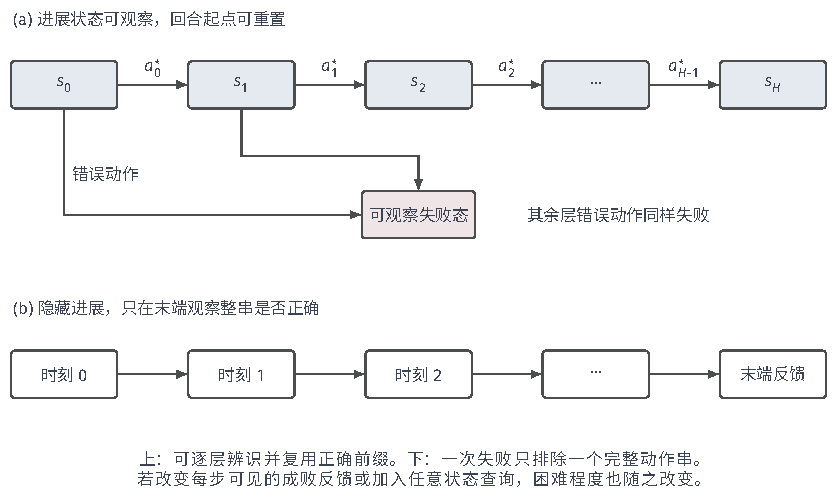
\includegraphics[width=141.750mm]{figures/10-reinforcement-learning/01-problems-and-solving/tikz/rl-learning-combination-lock.pdf}
  \caption{组合锁的难度取决于可观察性与访问方式。上图能观察正确进展或失败状态，只允许回合起点重置；下图把两者隐藏为同一观测，仅整串正确时给终点奖励。后者不是前述完全可观测表格MDP协议。}
  \label{fig:rl-learning-combination-lock}
\end{figure*}

具体地，设每层$n_A$个动作、恰有一个正确动作，确定性转移，错误进入可观察的失败态，下一回合可重置到链首。记住已经验证的前缀后，每层至多试$n_A$个动作，每次走至该层耗$O(H)$步，便有$O(n_AH^2)$步的直接辨识策略；若还有任意状态生成模型查询，连重放前缀也可省去。逐步均匀随机策略偶然成功的概率是$n_A^{-H}$，但这是该策略的表现，不是所有学习算法的下界。

若改成每步只观察时间、失败与进展状态隐藏、非末端奖励均为0，未知正确动作串从$n_A^H$个可能串中均匀选出，那么一次失败仅排除本次完整尝试。每回合最多验证一个串，固定成功概率需要$\Omega(n_A^H)$次尝试。这个教学问题族明确限制了反馈和重置能力；改变成可观察状态或允许查询隐藏状态，论证即不成立。

组合锁改变了观测条件。若仍保留完全可观测的标准设定，也能通过随机奖励的微小差异产生辨识成本。我们构造两个只有一步的环境：近优输出必须选不同动作，单次奖励却难以区分环境。下面将决策要求转换成统计检验，给出可完整计算的样本下界。

两个环境的下界思路与通常估计相反。我们先要求输出必须在两个环境中作出不同选择；再考察训练记录中的动作与奖励能否可靠地区分两个环境。如果大量记录在两环境中仍很相似，就不可能同时高概率选对。这把“策略近优”变成一个环境辨识任务，随后用记录分布的KL计算最多能积累多少证据。

\begin{theorem}[一步决策的辨识下界]
  \label{thm:rl-learning-two-instance-lower}
  设$H=1$、只有一个非终止状态和两个动作。环境$M_+$、$M_-$中动作2奖励均为Bernoulli$(1/2)$，动作1奖励分别为Bernoulli$(1/2+\Delta)$与Bernoulli$(1/2-\Delta)$，其中$0<\Delta\leq1/4$。算法可根据已见历史自适应选择动作，内部随机源在两环境中相同且独立于环境随机性；给定抽样前历史与当前动作，下一奖励仍服从该动作的指定分布。共取得$n\geq1$个奖励反馈后，算法输出任意随机策略。
  若对两环境都以至少$1-\delta$的概率输出$\epsilon$近优策略，其中$\epsilon=\Delta/4$、$0<\delta<1/4$，则
  \[
     n\geq\frac{1}{16\Delta^2}\log\frac1{4\delta}
       =\frac{1}{256\epsilon^2}\log\frac1{4\delta}.
  \]
\end{theorem}

\begin{proof}
  令$\widehat p$为输出策略选择动作1的概率。在$M_+$中$\epsilon$近优要求$\widehat p\geq3/4$；在$M_-$中要求$\widehat p\leq1/4$。故事件$E=\{\widehat p>1/2\}$给出两环境检验，且
  $\mathbb P_+(E^c)+\mathbb P_-(E)\leq2\delta$。

  设$\mathbb P_+,\mathbb P_-$为完整交互记录连同算法随机性的分布。条件于过去，算法使用同一动作选择机制；只有动作1的奖励分布不同。KL的链式法则因此给出
  \[
   D_{\mathrm{KL}}(\mathbb P_+\|\mathbb P_-)
    =\mathbb E_+[N_1(n)]\,
       \operatorname{kl}(1/2+\Delta,1/2-\Delta)
    \leq16n\Delta^2.
  \]
  最后一步利用$\Delta\leq1/4$和
  $\operatorname{kl}(1/2+\Delta,1/2-\Delta)
   =2\Delta\log[(1+2\Delta)/(1-2\Delta)]\leq16\Delta^2$。
  两分布检验不等式
  $\mathbb P_+(E^c)+\mathbb P_-(E)
       \geq\tfrac12e^{-D_{\mathrm{KL}}(\mathbb P_+\|\mathbb P_-)}$
  于是推出$2\delta\geq\tfrac12e^{-16n\Delta^2}$，移项即得结论。
\end{proof}

证明把三个步骤接在一起：奖励均值只差$2\Delta$使单次观测KL为$O(\Delta^2)$；近优策略却必须作出不同选择；检验错误概率将两者连接成样本下界。这里使用的换测度与顺序辨识思路也见最佳臂识别的原始分析，但上面的常数和$\epsilon=\Delta/4$是本书对这一教学问题对的直接推导\scite{rl3-kaufmann2016complexity}

该下界只证明一个状态、两动作、一步任务中已经需要$\epsilon^{-2}$量级奖励样本，不声称导出了前述所有$n_S,n_A,H$因子。多状态MDP下界还需构造多个必须分别辨识的局部选择，并分析访问这些选择与长期收益放大的关系。算法渐近收敛与此不矛盾：对奖励有差异的动作不断采样，最终可以区分两个环境，并不回答在$n$次反馈内能否可靠分清。

\begin{table*}[t]
  \centering
  \small
  \begin{tabularx}{\linewidth}{>{\raggedright\arraybackslash}p{26mm} >{\raggedright\arraybackslash}X >{\raggedright\arraybackslash}X}
    \toprule
    障碍 & 证据要求 & 能从中得出什么 \\
    \midrule
    记录不能区分环境 & 固定访问协议，构造难区分环境及检验下界 & 任何计算能力都不能凭不足的交互记录达到指定保证 \\
    样本有效但计算昂贵 & 有限样本算法依赖枚举大候选类或难解优化 & 当前构造不高效；若要断言所有算法都计算困难，还须规约或计算假设 \\
    计算高效但条件更强 & 如已知线性特征、合法线性转移与可执行动作最大化 & 在该结构族可同时控制交互样本量与计算量，不代表一般网络满足条件 \\
    \bottomrule
  \end{tabularx}
  \caption{可识别性、样本量与计算的边界。算法有昂贵子步骤不等于已经证明计算下界，预言机模型也必须与实际运行成本区分。}
  \label{tab:rl-learning-statistical-computational}
\end{table*}

表\ref{tab:rl-learning-statistical-computational}区分记录可识别、样本充分与计算可行三种判断。OLIVE展示一般结构下的样本可行性，LSVI-UCB在更明确的线性条件下提供可实现的更新，两环境下界则限制任何算法的奖励或转移样本需求。它们各自回答一个问题；只有把访问能力、函数类、目标精度和计算方式一起写出，才有可比较的“可学习”结论。

% Outline: 3.8
\section{算法评估和比较}
\label{sec:rl-learning-evaluation}

实验需要把前述访问能力、表示和预算落实到可复核配置。同一任务上更高的测量回报，可能来自更新机制，也可能来自更多真实交互训练记录、计算、调参或部署搜索。比较前应明确这些差别和评价目标，再报告对应预算下的回报及不确定性；否则一条较高曲线不能区分这些解释。

% Outline: 3.8.1
\subsection{数据与计算预算}
\label{sec:rl-learning-budget}

一条真实转移可以被DQN多次重放，也可以先训练模型，再产生很多合成经验。若只报“训练步”，就会把真实交互样本采集和重复计算混在一起，无法判断样本利用率或运行成本。表\ref{tab:rl-learning-budget-units}分别计真实转移、优化更新、抽样条数和模型查询，训练与部署也单列。

\begin{table*}[t]
  \centering
  \small
  \begin{tabularx}{\linewidth}{>{\raggedright\arraybackslash}p{27mm} >{\raggedright\arraybackslash}X >{\raggedright\arraybackslash}X}
    \toprule
    预算量 & 建议计数方式 & 常见误读 \\
    \midrule
    真实环境步 & 累计实际环境转移；并行环境按各自转移数相加 & 一次向量化调用不等于一次转移，动作重复后的帧数另记 \\
    梯度步 & 按优化器更新次数，并分开行动者、评论家、模型 & 两个评论家的更新不能与单个网络的一步含混合计 \\
    重放比例 & 同时报$U/N_{\mathrm{env}}$及$UB/N_{\mathrm{env}}$，$U$为更新数、$B$为批量 & 前者是更新次数比，后者是抽样条数比，数值相差$B$倍 \\
    模型样本 & 合成转移数、分支起点数与滚动长度分别记录 & 合成100万条不等于真实交互100万次 \\
    墙钟时间 & 固定硬件、并行度，分别记录采集、训练、评价及总耗时 & 只报网络更新时间会漏掉规划、仿真和轨迹采集等待 \\
    参数及内存 & 报可训练参数、目标网络与模型集成数量、峰值内存 & 相同参数数不等于相同计算，回放也占资源 \\
    部署预算 & 每次决策的模型查询、候选数、延迟分位数与硬件 & 训练时省样本可能换来每次动作的大量搜索 \\
    \bottomrule
  \end{tabularx}
  \caption{真实交互记录、记录重放与计算的不同单位。$U,B$随阶段变化时应按各批实际大小累加，不只报一个最终配置值。}
  \label{tab:rl-learning-budget-units}
\end{table*}

可以在基准网格上比较表格Q-learning与学习模型的Dyna，先固定相同的状态、动作、奖励、终止与起点规则。Dyna的模型只能用已取得经验拟合，不能暗中访问本书给出的真实转移表。两者最终都按约定贪心策略部署，探索和学习率的搜索预算相同；Dyna另报告每次真实转移后的模拟备份数。这里选择两种方法只是给出可复现的实验设计，不预先断定哪一个获胜。

一种预算视角固定真实交互数$N_{\mathrm{env}}$：在相同检查点冻结策略，用不进入训练缓冲的独立测试回合估计$J$，比较相同真实环境转移预算下的决策质量。另一种固定总计算资源与墙钟期限：把模型拟合、模拟备份和真实环境执行都计入，比较期限内得到的策略。前者允许算法多花计算提高样本利用率，后者则要求为这些计算付出代价。两种比较回答不同问题，结果不必一致。

部署成本另外测量。网格中两者都可查表选动作；若改成MPC与SAC比较，每次MPC动作的候选搜索应计入部署预算，而SAC的训练开销不应被挪进这一指标。在线更新若与动作生成共享设备，还要报告它是否影响控制延迟。

图\ref{fig:rl-learning-evaluation-protocol}给出两张曲线的作图协议，不包含实验结果。可预先约定20个独立训练种子、每个检查点100个独立测试回合；这些是教学协议的设定值，不是已经完成的运行。第$m$个种子在检查点的测试均值记为$\overline G_m$，保存
$(N_{\mathrm{env}},t_{\mathrm{wall}},\overline G_m)$及测试原始回报，同一检查点分别投到两个横轴，图例始终使用同一算法名与线型。没有实测训练与评价记录时不画领先曲线，也不以手绘趋势代替测量。

\begin{figure*}[t]
  \centering
  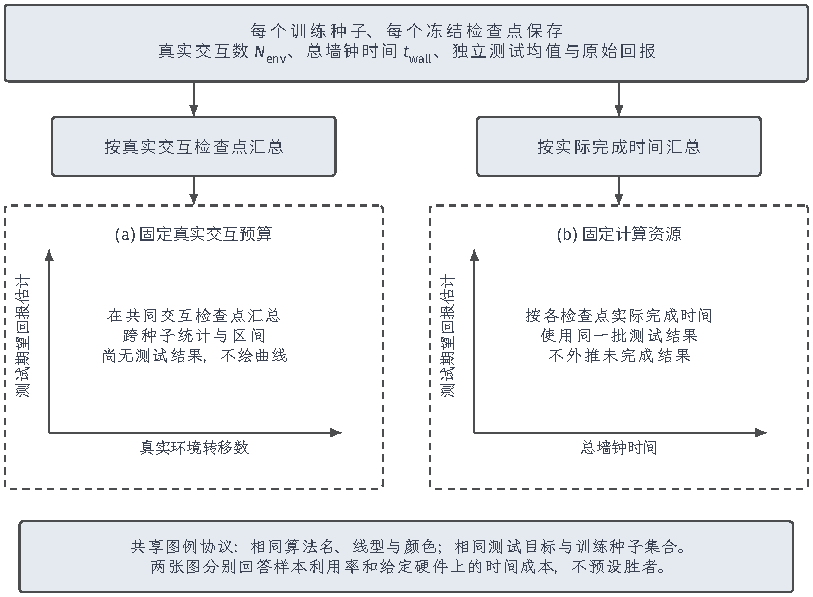
\includegraphics[width=137.615mm]{figures/10-reinforcement-learning/01-problems-and-solving/tikz/rl-learning-evaluation-protocol.pdf}
  \caption{两种预算视角的作图协议，非实验曲线。同一检查点记录同时保留交互数、墙钟时间与测试统计，分别汇总后形成交互预算和时间预算两个视图；方法标识、测试目标和抽样单位保持一致。取得实测训练与评价记录前不填曲线、误差带或排名。}
  \label{fig:rl-learning-evaluation-protocol}
\end{figure*}

画学习曲线还应预先约定插值规则。不同种子的检查点不齐时，可在共同交互预算上使用最近已完成策略，不把尚未达到的结果外推到较小预算；时间轴同理。是否平滑、平滑窗口、失败运行与提前终止如何显示，都要留在作图配置中。曲线下面积若被用作汇总，积分区间与横轴单位也是指标定义的一部分。

% Outline: 3.8.2
\subsection{统计报告与模型选择}
\label{sec:rl-learning-statistical-report}

固定一个训练后的策略测试1000回合，主要减少其环境回报估计的波动；重新训练1000次则还能观察初始化、探索和优化导致的策略差异。要评价算法而非一次幸运训练，必须分开这两个抽样层次，并明确置信区间覆盖哪一种平均性能。这里的学习结果是冻结策略，比较整个学习规则时则重新采集训练记录并重新运行训练程序；两者的期望分别对测试轨迹与训练过程取平均。只有在声明的抽样协议下，独立测试回合才估计对应策略的期望回报，不能把同一训练记录上的自举损失当作测试风险。训练模型与学习规则的两层评价可参考\BookChapterRef{chap:statistical-learning-framework}{卷3《基础、理论与可信性》中讨论机器学习理论基础的章节}。

\Needspace{8\baselineskip}
记第$m$个独立训练运行的冻结策略为$\pi^{(m)}$，第$n$次独立测试回报为$G_{m,n}$。先在每个策略的$N_{\mathrm{test}}$个回合内平均，估计这个产物的期望回报；再对$M$个训练运行平均，估计整个训练流程的平均性能：
\[
 \overline G_m=\frac1{N_{\mathrm{test}}}
                    \sum_{n=1}^{N_{\mathrm{test}}}G_{m,n},\qquad
 \overline G=\frac1M\sum_{m=1}^{M}\overline G_m .
\]
$G_{m,n}$是一次轨迹结果，$\overline G_m$估计这个训练产物的期望性能，$\overline G$估计训练流程随机运行后的平均性能。置信区间应说明覆盖哪一个对象。表\ref{tab:rl-learning-statistical-units}对应这三个层次。

\begin{table*}[t]
  \centering
  \small
  \begin{tabularx}{\linewidth}{>{\raggedright\arraybackslash}p{26mm} >{\raggedright\arraybackslash}X >{\raggedright\arraybackslash}X}
    \toprule
    抽样单位 & 主要随机性与报告量 & 不能替代的统计工作 \\
    \midrule
    单次测试轨迹 & 初始状态、环境噪声和策略采样；报告回报、长度或成功事件 & 一条幸运轨迹不代表该策略的期望性能 \\
    固定训练产物 & 多测试回合的均值与区间 & 不反映重新训练是否会失败 \\
    独立训练运行 & 种子间分布、均值或稳健汇总及区间 & 增加同一种子的测试回合不能消除训练方差 \\
    多任务基准 & 每任务分数、明确归一化后的汇总及性能分布 & 同一模型跨任务测量可能相关，不能当成全部独立样本 \\
    \bottomrule
  \end{tabularx}
  \caption{实验统计的抽样单位。种子列表、测试环境随机数与任务抽样分别记录，置信区间不能只写一个百分比而不说明覆盖对象。}
  \label{tab:rl-learning-statistical-units}
\end{table*}

两层抽样的差别可以量化。若训练产物的真实期望回报方差为$\tau^2$，给定训练产物的轨迹方差再对产物平均为$\sigma^2$，不同训练运行相互独立，且给定各自产物后测试轨迹条件独立同分布，则总方差公式给出
\[
 \operatorname{Var}(\overline G)
   =\frac{\tau^2}{M}
      +\frac{\sigma^2}{M N_{\mathrm{test}}}.
\]
增加$N_{\mathrm{test}}$只压低第二项。学习曲线的相邻检查点来自同一次训练，具有相关性；逐点区间不是“整条曲线同时被覆盖”的置信带，不能用每点95\%宣称整条曲线有95\%覆盖。

取一个教学方差配置$\tau^2=0.04,\sigma^2=0.25$，用$M=5$个训练运行、每个测试100回合，整体均值方差为$0.04/5+0.25/(5\times100)=0.0085$。把每个策略的测试增加到1000回合，只降至$0.00805$；保持100测试回合、把独立训练增加到20次，则降至$0.002125$。这些数说明当训练波动占主导时，反复测试同一模型不能代替重新训练；它们不是某个算法的实测方差。

最少应同时保留学习曲线、预先约定的最终检查点和全部运行的最终分数。跨任务平均前要说明归一化；均值敏感于极端高分，中位数可能掩盖大幅改善或退化，四分位均值（interquartile mean, IQM）取排序后中间50\%分数的平均，提供另一种稳健汇总，但它们没有共同的“正确排名”。

还可用性能分布曲线比较不同分数区域。这里固定一组$M_{\mathrm{task}}$个基准任务，先等概率抽一个任务，再按相同训练协议独立运行该任务的算法，记录预定最终检查点的归一化分数$X$；归一化所用参照也固定。曲线为$\mathbb P(X>\tau)$，表示这一任务与运行混合总体中超过阈值$\tau$的比例，而不是尚未指定的新任务总体。若任务$d$有$M_d$个最终分数$x_{d,m}$，其分层经验估计为
\[
  \widehat{\mathbb P}(X>\tau)
    =\frac{1}{M_{\mathrm{task}}}\sum_{d=1}^{M_{\mathrm{task}}}\frac1{M_d}
       \sum_{m=1}^{M_d}\mathbf1\{x_{d,m}>\tau\}.
\]
每个任务的总权重相同，避免运行较多的任务自动占更大权重；所有$M_d$相同时才等于将全部分数等权合并的尾频率。在同一任务集、预算和归一化下比较曲线，才能判断优势发生在哪些阈值区域。

区间重抽样也应匹配目标。若任务集合固定，按任务分层重抽各任务的训练运行；若关心新任务总体，还需说明任务抽样分布并在外层重抽任务。同一多任务训练产物的多个分数需以整组为单位保留相关性。少量种子下，任何区间估计仍可能很不稳定，应公开原始分数，而不是让一个窄色带制造精确感。Agarwal等人的研究系统讨论了深度强化学习少运行数评价中的区间、IQM和性能分布问题\scite{rl3-agarwal2021precipice}

\begin{example}[挑最好检查点造成的偏差]
  \label{ex:rl-learning-checkpoint-selection}
  假设两个检查点的真实测试均值都为$0.6$，各自的测量误差独立且以相同概率为$\pm0.1$。预先固定最后一个检查点，报告值的期望仍为$0.6$。若看完两次测试后挑较高者，则仅在两次都低时报告$0.5$，其他情形报告$0.7$，所以报告值期望为
  \[
    \frac14(0.5)+\frac34(0.7)=0.65.
  \]
  被选策略的真实均值仍是$0.6$。这$0.05$来自选择噪声，没有任何策略改善。
\end{example}

因此“最好检查点”可以是明确的模型选择协议，却不能在同一批测试轨迹样本上既选又报无偏性能。固定调参候选数、验证预算与选模规则，选择之后另用未参与选择的测试回合评估；若反复查看测试集并改变超参数，测试集已承担验证功能，应另留最终测试。第\ref{sec:rl-learning-dqn}节提到的Rainbow最好快照应按其原协议理解，不与固定最后检查点悄然混比。

消融也需相同预算。去掉组件后若释放大量计算，应说明是保持其他更新次数不变，还是把省下的计算重新分配；前者更接近固定实现条件下的组件作用，后者更接近固定资源下的系统比较。对失败运行不能只删去低分种子，算法性失败应按预先约定纳入分布；基础设施故障的重跑条件和次数另记。

% Outline: 3.8.3
\subsection{基准协议与复现边界}
\label{sec:rl-learning-benchmark-protocol}

使用同名环境也可能取得不同观测字段、执行不同动作或优化不同目标。以ALE为例，像素观测与模拟器内部状态记录属于不同的观测接口；动作重复、黏滞动作、随机起始空操作和生命损失处理还会改变动力学或回合边界。黏滞动作按规定概率继续上一动作，因而固定请求串不再机械复现同一轨迹。比较Atari结果时，需要记录ALE版本、ROM校验值、包装器和黏滞概率，才能确定两种方法面对的是否为同一协议\scite{rl3-machado2018ale}

Procgen有16个程序生成的游戏环境，核心协议之一是限制训练关卡种子，再在未用于训练的关卡上评价。训练与测试关卡重合时测的是另一种泛化问题；难度分布、关卡数、种子区间和版本都要记录。原论文对样本效率和泛化分别给出协议，不能把无限关卡训练与有限关卡训练的分数混在一起\scite{rl3-cobbe2020procgen}

\Needspace{20\baselineskip}
连续控制还需区分状态输入与像素输入、控制周期与底层物理仿真步长、动作重复、奖励缩放以及失败终止。DeepMind Control Suite与Gym中的相近身体模型未必有相同奖励、动作频率或终止条件，名字相似并不能建立直接可比性。其环境定义和任务设计应以具体版本为准\scite{rl3-tassa2018control}

\begin{table*}[t]
  \centering
  \small
  \begin{tabularx}{\linewidth}{>{\raggedright\arraybackslash}p{21mm} >{\raggedright\arraybackslash}X >{\raggedright\arraybackslash}X >{\raggedright\arraybackslash}X}
    \toprule
    基准 & 可见观测字段与动作接口 & 随机性与划分 & 终止及版本记录 \\
    \midrule
    ALE & 像素观测或模拟器内部状态记录、帧堆叠、动作集合、动作重复 & 黏滞动作、随机起始、训练与测试随机种子 & 真正游戏结束、生命损失包装、时间上限；ALE版本、ROM哈希 \\
    Procgen & 像素、动作映射、包装器与网络输入处理 & 训练关卡数、种子区间、未见关卡及难度分布 & 回合结束与截断；包版本、游戏配置、关卡生成种子 \\
    连续控制 & 状态或像素、动作范围、控制频率与重复 & 动力学随机性、初始分布、任务或扰动划分 & 失败终止与时间上限；仿真器、模型文件及任务版本 \\
    \bottomrule
  \end{tabularx}
  \caption{影响算法可读取的观测字段、动力学或目标的基准协议。具体概率和重复次数应从实际配置读取，不把某个流行默认值写成基准的唯一规则。}
  \label{tab:rl-learning-benchmark-settings}
\end{table*}

表\ref{tab:rl-learning-benchmark-settings}中的时间上限尤其容易改变学习目标。沿用第\ref{chap:rl-overview}章的区别，真实终止说明任务后继回报为0；采样截断可能只表示当前记录到此为止。设基准网格中一条非终止转移奖励$-0.04$，后继估值$0.8$，$\gamma=0.9$，若此处只是采样达到时间上限，正确自举目标为$0.68$；错当终止则变成$-0.04$，每次都漏掉$0.72$。若任务本来就定义为到这个时限结束，则零自举才符合目标，且剩余时间通常要进入决策状态。

实现中应分别保存\texttt{terminated}与\texttt{truncated}的含义，并按任务目标确定自举掩码。自动重置的向量环境还须使用截断前的最终观测，不能把下一回合重置后的观测当成这条转移的后继。时间上限的两种语义及其对状态与自举的影响，有专门的原始分析\scite{rl3-pardo2018timelimits}

跨游戏原始分数的单位不同，不能直接把数值大小当成统一性能。若用随机与人类参照对每个游戏缩放，就需要同时固定参照值和测量协议。以ALE常见的人类归一化分数为例，
\[
  S_{\mathrm{HN}}
   =\frac{S_{\mathrm{agent}}-S_{\mathrm{random}}}
          {S_{\mathrm{human}}-S_{\mathrm{random}}}.
\]
必须提供每个游戏的人类与随机参照值及其测量协议。若分母很小，少量原始分差会被放大；若参照顺序反常或分母为0，应说明排除或替代规则，不能直接平均。教学值
$S_{\mathrm{agent}}=30,S_{\mathrm{random}}=10,S_{\mathrm{human}}=50$
对应$0.5$，不是原始得分的“50\%”；它表示从随机到人类参照差距的一半。是否截断到某范围也会改变跨任务汇总，需明确报告。

\begin{table*}[t]
  \centering
  \small
  \begin{tabularx}{\linewidth}{>{\raggedright\arraybackslash}p{28mm} >{\raggedright\arraybackslash}X}
    \toprule
    复现记录 & 最少需要保存的内容 \\
    \midrule
    代码与配置 & 提交标识、依赖锁定、环境与包装器版本、全部实际展开后的超参数 \\
    训练记录、评价样本与随机性 & 真实交互记录与模型合成转移的来源及条数、训练与评价种子、初始分布、训练测试划分 \\
    更新语义 & 采样策略版本、目标网络与策略更新频率、终止掩码、重放比例及样本寿命 \\
    模型选择 & 候选与调参预算、验证集、停止及检查点选择规则、最终独立测试流程 \\
    失败处理 & 失败定义、原始结果、基础设施重跑规则与实际重跑次数 \\
    资源与产物 & 硬件、精度、并行度、墙钟和部署预算、模型检查点、逐运行日志与作图脚本 \\
    \bottomrule
  \end{tabularx}
  \caption{最小复现记录。分布式系统实现可在系统卷展开，但会改变采样分布或更新目标的接口必须在算法实验中说明。}
  \label{tab:rl-learning-reproducibility}
\end{table*}

表\ref{tab:rl-learning-reproducibility}不是附在论文末尾的形式清单：每一项都可能改变结论。例如异步采样器延迟会增大行为策略与目标策略的差别，回放保留期会改变访问分布，模型更新频率会改变合成经验的失配程度。采样服务与分布式存储怎样工程实现留给系统卷；这些实现选择对训练记录抽样分布和更新目标的影响，需要写入实验协议。

% Outline: 3.9
\section{本章小结}
\label{sec:rl-learning-summary}

回到章首网格问题，一次动作只能给出一次奖励和落点，我们既要用它估计长期后果，也要决定下一次去哪里取得证据。本章的四种组合给出了不同计算接口：直接更新价值或策略，或者先学模型，再用预测支持这些更新。表\ref{tab:rl-learning-final-interfaces}按主要更新对象和最终动作来源汇总；混合系统应沿交互记录、模型预测与训练目标之间的实际依赖解释，不能只凭出现了某个网络就归类。

\begin{table*}[t]
  \centering
  \small
  \begin{tabularx}{\linewidth}{>{\raggedright\arraybackslash}p{28mm} >{\raggedright\arraybackslash}X >{\raggedright\arraybackslash}X}
    \toprule
    主要接口 & 经验主要更新什么 & 最终动作主要来自哪里 \\
    \midrule
    无模型价值学习 & MC/TD回报、动作值与其函数表示 & 对动作价值贪心或按约定探索，如SARSA、Q-learning、DQN \\
    无模型策略优化 & 策略参数，通常另有评价策略的评论家 & 更新后的策略，如PPO、SAC；离策略校正与覆盖仍需检查 \\
    基于模型的价值学习与规划 & 动力学、奖励及规划需要的价值或搜索先验 & Dyna更新后的价值控制，或MPC、MuZero、TD-MPC的当前规划结果 \\
    基于模型的策略优化 & 动力学以及用模型梯度或合成转移记录训练的行动者、评论家 & 更新后的策略，如PILCO、Dreamer、MBPO；潜在状态推断仍可调用模型 \\
    \bottomrule
  \end{tabularx}
  \caption{四种组合共享探索、函数表示与时间抽象条件。混合系统按实际交互记录、模型预测与动作选择的依赖说明，不要求每个系统只学习一种对象。}
  \label{tab:rl-learning-final-interfaces}
\end{table*}

这些接口都处在同一反馈中。关键动作样本不足会使回报、转移或价值估计不可靠，估计误差又通过贪心选择或策略更新改变动作，新的访问分布进一步决定哪些误差能被修正。MC需要完整回报，因而通常等待回合结束；TD用一步奖励加后继预测，可以立即更新，却要处理自举误差。离策略评价复用旧策略的记录，还需保留行为动作概率并检查目标行为是否得到支持。它们对记录的要求不同，估计误差的来源也不同。双重采样反例提醒我们先核对损失是否对应目标；资格迹和优势估计改变信用传播长度，却不能补出未取得的奖励反馈。

是否得到可靠策略，取决于误差能否转到实际决策分布。统一动作值误差给出贪心策略损失界，低训练均方误差却可能漏掉关键岔路；性能差恒等式使用新策略占用下的优势，旧批次代理必须控制分布替代；模拟界需要奖励与转移误差覆盖被选策略，而搜索和想象优化恰会寻找高估区域。时间抽象同样保留这些要求：Option用$\gamma^K$维持原子时间目标，高层少做几次决策，并不意味着真实交互、内部控制学习或执行风险同比减少。

有限样本分析进一步把这些条件写成访问协议和问题结构。UCBVI依赖表格计数，LSVI-UCB依赖已知特征及线性奖励转移，OLIVE依赖候选误差的有限维分解；它们分别约束不同问题族，不能拼成任意神经算法的保证。实验相应地需要分别记录真实样本、重复更新、模型计算、选模和部署预算，并用独立训练运行区分训练波动与固定策略的测试波动。

因此，环境模型未知时仍可通过经验评价和改进策略，但一次更新可计算，尚不足以保证有限预算下近优。算法形式规定怎样利用记录，访问能力规定能取得什么记录，函数类规定不同状态动作的记录怎样共同约束价值或模型，预算则限制辨识和求解能做到哪里；四者共同决定策略保证的适用范围。后续各章改变观测与采集权限、奖励反馈、任务、参与者或行为要求，复用这里的部件时也需重新检查其交互记录来源、优化目标和保证条件。


\bookpart{信息与奖励受限的学习}{Learning with Limited Information and Reward}
\label{part:rl-information-and-reward}

\BookPartGuide{%
导航策略可能只取得局部相机观测，也可能只能使用过去保存的交互记录；即使允许继续行动，奖励也可能在任务结束时才出现，或只能由人工比较间接提供。这些限制作用于不同环节：观测决定行动前能够区分哪些状态，训练记录决定能够从哪些行为后果估计候选策略的价值，奖励则决定学习依据能否反映预定目标。本部分在前述规划与交互学习的共同设定上，分别研究这些限制。

第~\ref{chap:rl-information}章“信息受限下的强化学习”区分两类问题。状态不能完整观测时，需要由观测、过去动作及已见奖励形成可供决策的历史表示，或维护对可能状态的概率判断（信念）；交互记录固定时，则要检查行为策略的覆盖范围，判断候选策略的价值能否由现有训练样本确定，再讨论保守估计与受限的策略改进。两类限制同时出现时，历史表示能够预测后续观测，并不自动说明它足以评价未执行的动作。

第~\ref{chap:rl-reward}章“奖励受限下的强化学习”分别处理奖励难以观察、长期奖励难以归因和奖励与行为目标不匹配的问题。示范、偏好与可验证反馈提供不同的训练依据；奖励塑形、辅助任务和反馈模型改变学习信号，却各自需要检查策略是否仍然追求原定目标。新的策略产生新的交互记录后，还要重新核对反馈模型及其适用范围。

两章共同区分能否确定待估对象、有限训练样本下估计有多准确，以及已有学习规则能否求得合适策略。增加历史表示、补充训练记录或改变奖励反馈，解决的是其中不同的缺口；结论所需的覆盖、可识别性和目标一致性条件仍须分别成立。}


\chapter{信息受限下的强化学习}
\label{chap:rl-information}

一辆小车驶近岔路口，摄像头清楚地拍到了它的位置，控制器仍可能无法决定怎样转向。如果画面没有显示小车向哪一侧滑动，控制器需要借助过去的观测辨认当前运动状态。如果位置和速度都已知，但日志从未记录某种转向动作，学习者需要判断现有经验能否说明该动作的后果。前一种困难缺少用于辨认当前状态的观测线索，后一种缺少备选行动的后果证据。过去的观测可能帮助估计速度，但未必能精确恢复所有隐藏状态；记忆本身也不能告诉我们一个从未尝试的转向会怎样。反复训练可以重新利用日志，却不能把未记录的线索或未发生的试验变成已知事实。

第~\ref{chap:rl-learning}~章已经说明怎样从经验估计价值、优化策略和学习模型。本章考察这些方法在状态不全可见或只能使用固定日志时还能使用到哪一步。状态不可见时，我们要从当前观测转向完整历史，或构造保留动作后果预测依据的历史表示。经验固定时，首先要检查同一批可见记录是否仍允许两种不同的环境解释。例如，一个解释认为未试过的左转更好，另一个认为它更差；若两者都符合采集规律，日志本身就不能确定左转的价值。排除这种答案不唯一的困难以后，才有依据讨论基于有限训练记录的价值估计和策略改进。图~\ref{fig:rl-information-roadmap}~将这两条认识路径分开。离线部分可观测问题同时受到两类限制：既要检查历史中留下了哪些线索，也要检查收集者依据什么选择了日志中的动作。

本章先沿这两条路径分别推演，再检查它们同时存在时的条件。状态不全的路径从已有历史出发，研究怎样压缩、更新并用于动作比较；固定日志的路径从收集机制出发，研究哪些价值能确定、怎样估计，以及生成新策略时如何防止利用外推错误。允许少量新试验会改变证据来源，因此单独讨论其作用。所需概率计算主要是条件概率、加权平均和期望；新的识别条件会在对应问题中说明。

\begin{figure*}[htbp]
  \centering
  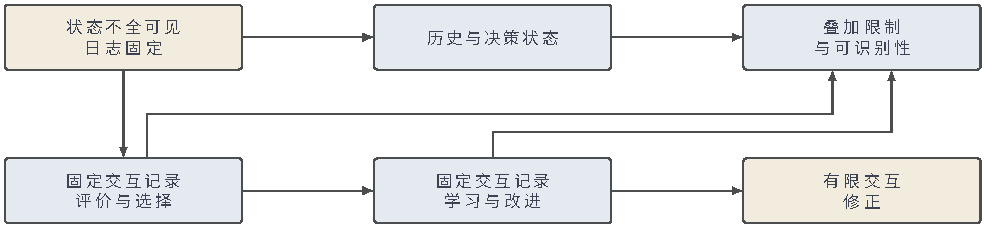
\includegraphics[width=166.857mm]{figures/10-reinforcement-learning/02-information-and-reward/tikz/rl-information-roadmap.pdf}
  \caption{本章的阅读依赖。箭头表示理解后项需要前项建立的概念，不表示算法的执行顺序。历史表示说明行动时能依据什么，固定日志上的策略评价说明已有经验能支持哪些判断；两者共同限制离线部分可观测问题中的策略结论。}
  \label{fig:rl-information-roadmap}
\end{figure*}

% Outline: 4.1
\Needspace{6\baselineskip}
\section{两类信息限制}
\label{sec:rl-information-limits}

% Outline: 4.1.1
\subsection{决策所依据的状态信息}
\label{sec:rl-information-state-information}

第~\ref{chap:rl-overview}~章的马尔可夫条件针对完整状态$s_t$：给定它和当前动作，就能描述下一步的条件分布，无须再查询更早的经历。摄像头取得的$o_t$只显示位置，未直接给出速度，给定同一画面和动作，后果仍可能随未见的速度而变化。因此，执行策略不能沿用直接依据$s_t$决策的规则，而要考虑此前已取得的记录。一步记录$(o_t,a_t,r_t,o_{t+1})$按真实交互时刻$t$排列：先看到$o_t$，再执行$a_t$，随后取得奖励$r_t$和下一观测。这个时间下标不表示训练中的梯度更新次数。

过去动作也应进入历史，因为同一对画面可以由不同控制输入产生。例如，看到小车位置没有改变，既可能是未施加动力，也可能是施力后遇到障碍；只存画面会把这两种经历合并。我们因此把每一步已经看见、已经执行、已经收到的内容按发生顺序一起保存，作为当前策略真正能读取的材料。

历史中也保留奖励，因为奖励可能帮助辨认状态。例如，碰撞后返回的奖励可以说明小车触及了画面中看不见的障碍；删去它，就可能丢掉下一次决策需要的线索。这里保留的都是已经发生的反馈，未来才揭示的状态或奖励不能提前交给当前策略。

\begin{definition}[决策历史]
  \label{def:rl-information-history}
  时刻$t$的完整记录历史按时间排列行动前已经取得的观测、动作和奖励，写为
  \[
    I_t=(o_0,a_0,r_0,\ldots,a_{t-1},r_{t-1},o_t).
  \]
  历史条件策略$\pi(a\mid I_t)$以行动前已获得的观测、动作和奖励为依据。当前观测策略仅依据$o_t$决策；长度为$L$的窗口策略仅保留最近$L$步记录，并须约定窗口在回合边界处怎样构造。
\end{definition}

\begin{example}[相同位置与不同记忆]
  \label{ex:rl-information-cue}
  考虑一个独立教学任务。小车的真实状态包括位置$x_t$和速度$v_t$，摄像头只给出位置。同样看到$x_t=0$时，若$v_t=1$，所需制动方向与$v_t=-1$时相反。为判断运动方向，可以比较相邻位置。在无噪声、采样间隔为1且速度在相邻采样间不变的简化条件下，$v_t=x_t-x_{t-1}$；两次位置观测足以恢复速度，单帧不能给出这个位移差。

  再考虑线索出现得更早的岔路任务。回合开始时，提示$c\in\{L,R\}$以相同概率显示；小车随后经过$L+1$步外观相同的走廊，途中只能前进，奖励均为0。出口处选中$c$指示的方向得1，选错得0。本例及后文均按不折扣的回合成功奖励比较，其期望就是成功概率，不采用默认折扣回报。完整历史策略可以记住提示，期望成功奖励达到1。最近$L$步窗口已经看不到提示，固定的前进动作也不能编码提示，因此这类策略的最好期望成功奖励为$1/2$。
\end{example}

在岔路任务中，窗口内的观测、动作和奖励记录对左右提示完全相同。任何只读该窗口的策略都只能给出同一动作概率：设它以概率$p$选左，成功概率为$(1/2)p+(1/2)(1-p)=1/2$。这个结果不取决于网络有多大，也不取决于$p$怎样训练；被删除的提示根本没有进入策略可读取的记录。保留一位左右记忆就足够，而不断重复读取相同走廊画面不提供新的左右提示。

位置任务只需多保留一帧，便能补出缺失的速度；岔路任务却说明，任意预先固定的窗口都可能因线索延迟更长而失效。表示是否足够，取决于它有没有保留能区分候选动作后果的观测、动作和奖励记录，而不是保留的历史记录序列单纯有多长。

% Outline: 4.1.2
\subsection{学习能够访问的经验}
\label{sec:rl-information-data-access}

现在让日志完整记录小车的位置和速度。如果收集者在某个状态从不向左转，我们仍可能不知道在那里左转会怎样。缺口不在单条记录的字段，而在整批记录涉及的行为。分析可用经验时，必须分别检查记录是否完整、收集行为覆盖了哪里，以及学习者能否主动补采样。

固定日志下，学习者可以重新抽取记录、计算梯度、拟合价值或模型，但这些操作的结果都依赖同一批原始证据。允许新交互时则不同：学习者可以真实执行过去没有尝试的动作，并看到它的结果。为比较这两种学习条件，需要把算法能算什么与算法能查询什么分开；下面的协议规定的是后者，包括用于选模或评价的真实调用。

\begin{definition}[经验访问协议]
  \label{def:rl-information-access}
  \term{固定经验}协议将可用材料限定为给定的有限交互记录组$D$及声明可用的采集元数据，训练和选模期间都不允许查询真实环境。\term{有限新增交互}协议允许在约定的轮次和预算内补充真实经验；每轮可执行的策略、重置权限和专家帮助权限均由协议规定。\term{持续在线交互}协议允许策略根据经验不断更新并继续采集交互训练记录，但重置、传感和测试权限仍须明确，不能据此假定可以从任意状态采样。
\end{definition}

固定日志即使回放一百万轮，真实访问过的状态和动作也不会增加，改变的只是算法利用这些记录的方式。学习模型生成一百万条模拟转移，同样没有新增真实查询。表~\ref{tab:rl-information-access}~沿用完整记录位置和速度的小车任务，对照交互权限改变后能够取得的证据。

\begin{table*}[htbp]
  \centering
  \small
  \begin{tabularx}{\linewidth}{p{20mm}XXXX}
    \toprule
    协议 & 记录字段 & 行为覆盖 & 主动采样权限 & 评价查询权限 \\
    \midrule
    固定经验 & 位置、速度、动作、奖励和回合边界 & 仅原日志的收集行为 & 无真实调用、无重置 & 只能离线估计；不能试跑候选 \\
    有限新增 & 原字段加策略版本、轮次和查询用途 & 原日志加预算内新增行为 & 每轮限定步数；重置单列计数 & 允许的测试也扣除预算 \\
    持续在线 & 同样记录状态与行为元数据 & 随收集策略持续变化 & 在可达轨迹上继续行动；任意状态重置仍需授权 & 独立测试记录不参与拟合或选模，查询成本单列 \\
    \bottomrule
  \end{tabularx}
  \caption{同一完全可观测小车任务中的三种经验协议。完整字段不能补齐未尝试的动作；可以继续交互，也不意味着可以像调用生成模型那样从任意指定状态采样。}
  \label{tab:rl-information-access}
\end{table*}

% Outline: 4.1.3
\subsection{观测完整性与新增交互权限的组合}
\label{sec:rl-information-two-axes}

小车能否取得完整状态，并不决定训练者能否继续驾驶它。只见位置的控制器可以被允许主动加减速，借反馈辨认运动方向；已经记录位置和速度的日志也可以禁止新增试验。表~\ref{tab:rl-information-two-axes}~将观测完整性与交互权限交叉排列，得到四种条件。

\begin{table}[htbp]
  \centering
  \small
  \begin{tabularx}{\linewidth}{p{18mm}XX}
    \toprule
    执行观测 & 可新增真实交互 & 只有固定经验 \\
    \midrule
    完整状态 & 位置、速度均可见，可继续控制小车 & 状态字段完整，但只能使用已有驾驶日志 \\
    部分观测 & 只见位置，需要历史，可主动探查 & 只见位置，需要历史，仅有固定轨迹 \\
    \bottomrule
  \end{tabularx}
  \caption{观测完整性与训练记录采集权限可以交叉组合。允许少量新增经验只放宽访问权限，不改变观测类型；这些部分观测任务的模型将在下节建立。}
  \label{tab:rl-information-two-axes}
\end{table}

历史压缩遗漏线索与日志未覆盖目标动作会导致不同的失败。两类限制同时存在时，还要核对日志保存的历史与采集者选择动作的依据，不能把一种限制的处理直接用于另一种限制。

% Outline: 4.2
\section{决策信息不完整下的强化学习}
\label{sec:rl-information-partial-observation}

% Outline: 4.2.1
\subsection{从当前观测扩展为可得历史}
\label{sec:rl-information-history-policy}

回到例~\ref{ex:rl-information-cue}~的出口：同一画面下，早期提示为左时应向左，为右时应向右。\term{观测混叠}（observation aliasing）就是不同决策处境对应同一个当前观测，因而仅凭该观测无法区分它们。完整隐藏状态可以满足马尔可夫条件，观测过程却未必满足；我们需要同时描述状态怎样演化、观测怎样产生。图~\ref{fig:rl-information-aliasing}~将这两种关系分开，也显示相同当前观测可以来自不同历史。

前章用一个状态变量同时表达“环境当前处于哪里”和“策略现在知道什么”。这里要把二者分开。小车的完整状态含位置与速度，摄像头给出的读数却可能只有位置；同一位置读数对应多种完整状态，不能再直接用观测代替状态作Bellman备份。环境仍从完整状态出发演化，我们另给一条观测生成规律，说明这一演化的哪些结果能够被控制器看见。动作还可能改变观测方式，如停下观察或主动倾听，因此反馈模型要保留动作条件。

\begin{definition}[有限部分可观测马尔可夫决策过程]
  \label{def:rl-information-pomdp}
  \term{部分可观测马尔可夫决策过程}（partially observable Markov decision process, POMDP）分别描述环境的隐藏状态和智能体取得的观测。设$S$、$\mathsf A$、$\mathsf O$分别为有限非空状态集、动作集和观测集，$\mu_0$为$S$上的初始分布，$H$为正整数时域；奖励取值于有限非空集$\mathcal R\subset\mathbb R$。

  初始观测核$K_{o,0}:S\to\Delta(\mathsf O)$在$s_0\sim\mu_0$后生成$o_0$。时刻$t=0,\ldots,H-1$，策略依据$I_t$选择$a_t$，环境随后生成$s_{t+1}$及反馈$y_{t+1}=(r_t,o_{t+1})$。令$\mathcal Y=\mathcal R\times\mathsf O$，将下一状态与反馈的条件分布合写为联合概率核$K:S\times\mathsf A\to\Delta(S\times\mathcal Y)$；对每个$(s,a)$，$K(s',y\mid s,a)\geq0$且$\sum_{s',y}K(s',y\mid s,a)=1$。其生成含义为
  \[
    K(s',y\mid s,a)
    =\mathbb P(s_{t+1}=s',y_{t+1}=y\mid s_t=s,a_t=a).
  \]
  对反馈求和得到转移核$T(s'\mid s,a)=\sum_yK(s',y\mid s,a)$；按奖励值加权所有后果，得到期望奖励
  $R(s,a)=\sum_{s',r,o'}rK(s',(r,o')\mid s,a)$。奖励有界，采用回报
  $\sum_{t=0}^{H-1}\gamma^t r_t$，其中$0\leq\gamma<1$，终端价值取0。
\end{definition}

联合核保留了奖励与观测在给定当前状态和动作后的相关性，只有满足相应独立性时，才可进一步分解为转移和观测模型。按照上述观测、奖励与历史记录约定，执行策略写作$\pi_t(a\mid I_t)$；仅使用当前观测的$\pi_t(a\mid o_t)$限制了可选择的策略。我们保留时刻$t$，因为有限时域中剩余时间也会影响动作选择，即使对隐藏状态的推断相同也如此。

\begin{figure*}[htbp]
  \centering
  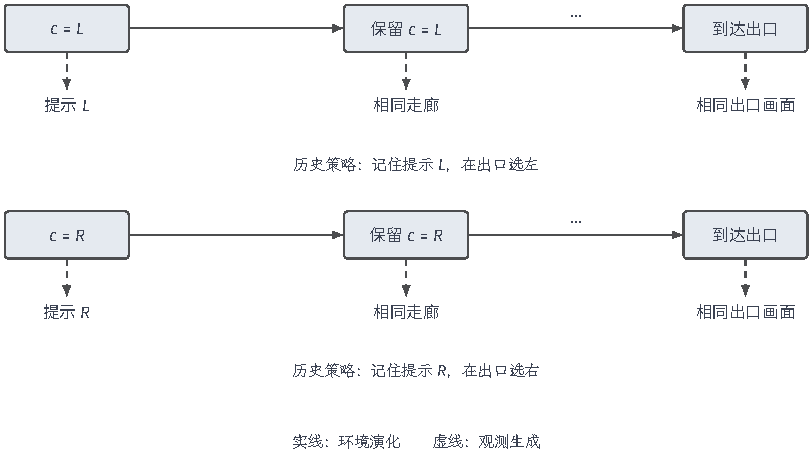
\includegraphics[width=137.534mm]{figures/10-reinforcement-learning/02-information-and-reward/tikz/rl-information-aliasing.pdf}
  \caption{早期提示任务中的两条可能轨迹。实线描述隐藏状态演化，虚线描述观测生成，途中固定为前进的动作未画出。出口画面相同，旁边单列的历史策略却因记住不同提示而选择相反方向；这些动作不属于观测。}
  \label{fig:rl-information-aliasing}
\end{figure*}

仿真器有时能在训练日志中给出$s_t$，帮助训练评论家或表示。但部署时若只能取得$o_t$，执行策略就不能读取这一特权状态，评价时也须提供部署真正可用的历史。要利用状态模型而不直接观测状态，可以推断当前状态的概率分布；下面的信念方法正是通过这一分布连接推断与决策，经典POMDP论述也采用这一思路\scite{rl1-kaelbling1998-pomdp}

% Outline: 4.2.2
\subsection{将可得历史压缩为决策状态}
\label{sec:rl-information-sufficiency}

完整历史保留了已记录的线索，但记录长度会随时间增长。下一次动作通常不需要逐字重读每个旧画面，只需要旧线索对当前状态判断留下的影响。模型已知时，可以为每个可能状态保存一个概率：过去动作先改变状态预测，新观测再改变各状态的相对可能性。这份分布称为信念状态（belief state），表示依据目前证据对真实状态的判断；它既压缩历史，又保留尚未排除的可能性。

如果把“障碍在左侧的概率为0.6”直接改成“障碍在左侧”，右侧仍有0.4概率这一可能性就被删掉了。碰撞成本很高时，这部分概率可能改变应选的动作。要说明保留完整分布为何足以支持控制，需要证明：预测奖励、更新状态推断和比较动作，都可以只使用信念完成。

\begin{definition}[信念状态]
  \label{def:rl-information-belief}
  给定有限POMDP，其隐藏状态集为$S$，策略按行动前可得的观测、过去动作与可见奖励历史$I_t$选择动作。对该过程生成律下具有正概率的可达历史$I_t$，\term{信念状态}（belief state）为
  \[
    b_t(s)=\mathbb P(s_t=s\mid I_t),\qquad
    b_t\in\Delta(S),
  \]
  其中$\Delta(S)$是$S$上的概率单纯形，即所有状态概率非负且总和为1的分布集合。$b_t$是给定历史后的后验分布，不表示另一个物理状态；只留下$\argmax_s b_t(s)$得到的点估计也不等于信念。
\end{definition}

推断从回合开始便已发生。对于具有正概率的初始观测$o_0$，按初始分布与观测似然加权并归一化，得到
$b_0(s)=\mu_0(s)K_{o,0}(o_0\mid s)/\sum_{\bar s}\mu_0(\bar s)K_{o,0}(o_0\mid\bar s)$；
仅当初始观测不改变关于初态的分布判断时，$b_0$才可直接取为$\mu_0$。

可以用带噪提示的教学变体核算初始更新。真实左右提示先验各为$1/2$，传感器以$0.8$概率报告正确提示。收到“左”时，“真实左且报告左”的概率为$0.5\times0.8=0.4$，“真实右却报告左”的概率为$0.5\times0.2=0.1$。报告左的总概率为$0.5$，归一化后真实左、右的概率为$0.8,0.2$。新观测增强了左的证据，却没有证明右不可能；再收到其他反馈时，还要继续更新这两个概率。

要证明压缩后没有丢掉最优决策所需的后果预测依据，不能只看这一次推断正确。还需检查三个操作是否都能从当前信念完成：预测一个动作带来的奖励和反馈，收到反馈后生成下一信念，按这些预测比较后续行为。下面的证明依次完成这三步，再用有限时域的反向归纳说明最优策略确实可以只读信念和时刻。

\begin{theorem}[精确信念对最优控制充分]
  \label{thm:rl-information-belief-sufficient}
  考虑定义~\ref{def:rl-information-pomdp}~中的已知有限POMDP，并假设动作选择仅依赖完整记录历史与独立的策略随机数。每个时刻$t$的最优历史价值都能写成$V_t^*(I_t)=U_t^*(b_t)$，且存在仅以$(t,b_t)$为依据的最优策略。
\end{theorem}

\begin{proof}
  先检查信念能否预测一个动作的后果。固定正概率历史$I_t$并选择$a$；由于动作只依据该历史和独立随机数，给定历史后的动作本身不再透露隐藏状态。按当前各状态的概率加权联合核，全概率公式给出
  \[
    \mathbb P(s_{t+1}=s',y_{t+1}=y\mid I_t,a)
    =\sum_s b_t(s)K(s',y\mid s,a).
  \]
  为预测可见反馈，将上式对隐藏的下一状态$s'$求和，得到
  $q(y\mid b_t,a)=\sum_{s,s'}b_t(s)K(s',y\mid s,a)$；将奖励取期望，得到
  $\bar R(b_t,a)=\sum_s b_t(s)R(s,a)$。反馈概率和奖励期望都由$(b_t,a)$确定。

  反馈出现后还需要更新推断。对$q(y\mid b_t,a)>0$的反馈，以其概率归一化状态与反馈的联合概率，贝叶斯公式给出
  \[
    b_{t+1}(s')
    =\frac{\sum_s b_t(s)K(s',y\mid s,a)}
           {q(y\mid b_t,a)}
    =:\tau(b_t,a,y)(s').
  \]
  新信念只需旧信念、动作和新反馈便可算出，这就是后验递推闭合；已经压缩的其余历史无需再读。零概率反馈不贡献期望，因此任意指定这些反馈上的$\tau$都不改变价值。

  最后用反向归纳检查最优动作比较。终点满足$V_H^*(I_H)=0$，可令$U_H^*(b)=0$。假设$t+1$时已有$V_{t+1}^*(I)=U_{t+1}^*(b(I))$；那么在$t$时选择$a$，当前奖励加上按可能反馈加权的最优继续价值为
  \[
    \bar R(b_t,a)
    +\gamma\sum_y q(y\mid b_t,a)
                      U_{t+1}^*(\tau(b_t,a,y)).
  \]
  上式仅依赖$b_t$与$a$。动作都来自有限动作集，按期望回报从中取最大值，便定义了$U_t^*(b_t)$并完成这一步归纳。在每个$(t,b)$处选取最大化动作，以固定规则处理平局，就构造出达到该值的信念策略。归纳到$t=0$，结论成立。
\end{proof}

这一结果说明最优控制不必保留信念以外的历史，并没有要求所有历史策略都在相同信念下选择同一动作。控制器可以故意按一个与未来无关的旧观测切换动作；这只是它使用了额外历史，不影响最优信念策略的存在。

上述构造需要已知模型；模型未知时，精确后验也不能直接计算。学习型潜在信念尝试用$\bm z_t$编码隐藏状态的不确定性。

信念记录的是隐藏状态概率；也可以换一个记录对象，直接保存“现在执行某串动作，会看到某串反馈”的概率。如果这些预测足以推算其他所需试验，就能直接比较动作后果，不必先恢复一套有语义名称的隐藏状态。指定动作是试验的条件，不是随机结果的一部分，这一区别会影响日志中应计算哪种概率。

另一种选择是\term{预测状态表示}（predictive state representation, PSR），用若干未来试验发生的预测概率概括历史。“试验”包含指定的未来动作和随后要观察的反馈，因此只预测收集策略自然产生的下一帧还不够。计算试验概率时，应按协议执行指定动作，再对环境反馈求概率，不能把行为策略恰好选择这些动作的概率乘进去。用日志条件频率估计试验概率时，还须说明所条件化的历史与采集随机化；仅筛出未来动作恰好匹配的记录，一般不足以完成这种校正。若这些概率能够递推所有相关试验，就可不必为隐藏状态赋予语义名称；表示是否有限维、能否从指定采集协议下的历史、动作和反馈记录学习，仍依赖结构条件\scite{rl4-littman2001-psr}

\begin{example}[动作试验概率与一次预测更新]
  \label{ex:rl-information-psr-test}
  令隐藏量$U\in\{0,1\}$在回合内保持不变，奖励均为0。执行动作$A$后观测为$U$，执行$B$后观测为$1-U$。可用“执行$A$后看到1”的概率$\zeta_t$概括当前历史；若$\zeta_t=0.3$，则“执行$B$后看到1”的概率为$0.7$。执行$A$并实际看到1后，更新为$\zeta_{t+1}=1$，随后执行$B$看到1的概率便为0。这个更新只需旧预测、执行动作和新观测。

  若采集者独立地以$0.2$概率选择$A$，日志中“选择$A$且看到1”的联合概率为$0.2\times0.3=0.06$；它包含采集动作的概率，不是执行$A$这一试验时看到1的概率$0.3$。
\end{example}

选择学习目标时，还要明确表示对什么问题充分。表~\ref{tab:rl-information-sufficiency}~分别考察未来反馈、固定策略价值和最优控制。例如，在两个隐藏状态中，“始终停止”的价值均为0，但向左、向右的奖励恰好相反。常数表示能准确预测停止策略的价值，却无法帮助选择转向动作。固定策略价值充分，不能据此推出改进所需的充分性。

\begin{table*}[htbp]
  \centering
  \small
  \begin{tabularx}{\linewidth}{p{25mm}XXX}
    \toprule
    充分性要求 & 必须保留的量 & 动作或策略范围 & 仍可丢失什么 \\
    \midrule
    未来反馈预测充分 & 各允许动作试验下的未来反馈联合分布与可递推状态 & 声明的全部试验，通常跨多个动作与时域 & 对这些预测无影响的历史细节与隐藏状态名称 \\
    给定策略价值充分 & 给定$\pi$和奖励下的条件期望回报 & 只要求该$\pi$的继续行为；还需说明执行时可读取的观测与历史 & 其他动作的价值、完整反馈分布 \\
    最优控制充分 & 允许策略类中达到最优值所需的动作比较与更新 & 所允许的控制行为；依赖任务与时域 & 不影响最优动作的预测细节 \\
    \bottomrule
  \end{tabularx}
  \caption{三种充分性对应不同问题。固定策略的回报预测正确，仍可能缺少评价其他动作或另一奖励函数所需的历史差别；已知POMDP中的精确信念则具有最优控制充分性的依据。}
  \label{tab:rl-information-sufficiency}
\end{table*}

% Outline: 4.2.3
\subsection{新观测到来后的决策状态更新}
\label{sec:rl-information-filtering}

信念充分性证明中，每次取得反馈都要生成新信念。实际计算时，给定已执行的$a_t$和收到的$y_{t+1}=(r_t,o_{t+1})$，先遍历可能的前态，用旧信念加权联合核，得到
$\widetilde b_{t+1}(s')=\sum_s b_t(s)K(s',y_{t+1}\mid s,a_t)$。这是下一状态与该反馈同时出现的概率，尚未归一化。再对所有下一状态求和，算出模型赋予该反馈的总概率；以它为分母，得到给定反馈后的状态分布：
\begin{equation}
  \label{eq:rl-information-bayes}
  b_{t+1}(s')
  =\frac{\sum_s b_t(s)K(s',y_{t+1}\mid s,a_t)}
         {\sum_{\bar s}\sum_s b_t(s)K(\bar s,y_{t+1}\mid s,a_t)}.
\end{equation}
这个条件分布只在分母为正时有定义。真实反馈若在模型中概率为0，滤波器便无法按上式归一化，需要检查模型或传感假设是否与实际过程失配。

若希望先预测状态、再单独用观测校正，就需要对联合核增加条件。假设
$K(s',(r,o')\mid s,a)=T(s'\mid s,a)K_o(o'\mid s',a)p(r\mid o',a)$，
这表示给定$o'$与$a$后，奖励不再改变对前后状态的条件分布判断。此时奖励项在分子分母中相同，可以约去；先对前态加权转移核，再按新观测的似然重新加权和归一化，得到
\begin{align}
  \label{eq:rl-information-predict-correct}
  b_{t+1}^{-}(s')&=\sum_sT(s'\mid s,a_t)b_t(s),\\
  b_{t+1}(s')&=
  \frac{K_o(o_{t+1}\mid s',a_t)b_{t+1}^{-}(s')}
       {\sum_{\bar s}K_o(o_{t+1}\mid\bar s,a_t)b_{t+1}^{-}(\bar s)}.
  \nonumber
\end{align}
碰撞奖励若由隐藏状态决定且提供了观测以外的线索，这一分解条件便不成立，更新时仍须保留奖励。

预测—校正也可以用于连续位置。此时不能逐个列出所有实数状态；若后验为高斯分布，就用均值$m_t$记录中心，用方差$\Sigma_t$记录不确定性。执行已知位移后，预测中心跟着移动；过程噪声增大预测方差。传感器再提供另一份带噪测量，校正应综合预测与测量的精度，而非总相信较新的那个数。

\begin{example}[一次标量滤波]
  \label{ex:rl-information-kalman}
  用标量教学系统$x_{t+1}=x_t+u_t+w_t$、$o_{t+1}=x_{t+1}+v_{t+1}$核算一次更新。给定已取得的历史，设当前状态的后验为$\mathcal N(m_t,\Sigma_t)$。过程噪声$w_t$与观测噪声$v_{t+1}$相互独立，也独立于当前状态和已取得的历史，均为零均值高斯量，方差分别记为$W,N$；另行记录的奖励不提供观测以外的状态线索。当前$m_t=0$、$\Sigma_t=1$，令已知控制量$u_t=1$、$W=N=1$，随后观测到2。状态预测为$m^-_{t+1}=1$、$\Sigma^-_{t+1}=2$，由此算得增益$2/3$。观测比预测大1，校正得到$m_{t+1}=1+(2/3)(2-1)=5/3$、$\Sigma_{t+1}=2/3$。方差尚未归零，所以$5/3$是后验均值，不是已知的真实位置。
\end{example}

这次增益$2/3$并非任意平均。预测位置方差为2，测量噪声方差为1，测量更精确，所以校正把两者之差的$2/3$加到预测上。若测量噪声方差改为100，其他条件相同，增益变为$2/(2+100)=1/51$，相同的测量偏差只会带来很小修正。下面的卡尔曼公式推广这种按误差协方差决定权重的关系，并明确它在哪些模型条件下是精确后验。

有限状态可以直接更新每个状态的概率；连续状态则需要适合其分布结构的表示。线性高斯模型在下述条件下使后验保持高斯，只需存储均值和协方差。设
$\bm x_{t+1}=\bm A\bm x_t+\bm B\bm u_t+\bm w_t$，
$\bm o_{t+1}=\bm C\bm x_{t+1}+\bm v_{t+1}$；
状态、控制输入与观测分别属于$\mathbb R^{d_x}$、$\mathbb R^{d_u}$和$\mathbb R^{d_o}$。
$\bm A\in\mathbb R^{d_x\times d_x}$传播状态，$\bm B\in\mathbb R^{d_x\times d_u}$将控制输入映到状态变化，$\bm C\in\mathbb R^{d_o\times d_x}$将状态映到观测。初始状态为高斯；所有时刻的过程噪声$\bm w_t$、观测噪声$\bm v_{t+1}$与初始状态相互独立，两类噪声均为零均值高斯量，协方差分别为$\bm W\in\mathbb R^{d_x\times d_x}$和$\bm N\in\mathbb R^{d_o\times d_o}$。控制输入$\bm u_t$只依据行动前已得历史和与环境独立的策略随机数，因此当前过程噪声与新观测噪声不含历史相关项；另行记录的奖励暂不改变只依据观测形成的状态后验。当前后验为
$\mathcal N(\bm m_t,\bm\Sigma_t)$时，\term{卡尔曼滤波}（Kalman filter）先传播均值和协方差，再用实际观测与预测观测的差修正它们。预测与校正递推为
\begin{align}
  \label{eq:rl-information-kalman}
  \bm m^-_{t+1}&=\bm A\bm m_t+\bm B\bm u_t,&
  \bm\Sigma^-_{t+1}&=\bm A\bm\Sigma_t\bm A^\top+\bm W,\nonumber\\
  \bm L_{t+1}&=\bm\Sigma^-_{t+1}\bm C^\top
     (\bm C\bm\Sigma^-_{t+1}\bm C^\top+\bm N)^{-1},\nonumber\\
  \bm m_{t+1}&=\bm m^-_{t+1}
       +\bm L_{t+1}(\bm o_{t+1}-\bm C\bm m^-_{t+1}),\nonumber\\
  \bm\Sigma_{t+1}&=(\bm I-\bm L_{t+1}\bm C)\bm\Sigma^-_{t+1}.
\end{align}
式中$\bm I$为$d_x$维单位矩阵，增益$\bm L_{t+1}$为$d_x\times d_o$矩阵，将观测差映为状态修正。创新$\bm e_{t+1}=\bm o_{t+1}-\bm C\bm m^-_{t+1}$就是实际观测相对预测观测的差；给定已有历史和当前控制输入，其协方差为
$\bm S_{t+1}=\bm C\bm\Sigma^-_{t+1}\bm C^\top+\bm N$，
状态预测误差与创新的交叉协方差为$\bm\Sigma^-_{t+1}\bm C^\top$。
在线性校正中，最小均方误差要求校正后的误差与创新正交，因而增益满足正规关系
$\bm L_{t+1}\bm S_{t+1}=\bm\Sigma^-_{t+1}\bm C^\top$。
这里要求$\bm S_{t+1}$可逆；解该关系便得到式中的增益，而不是任意选取预测均值与新观测的权重。联合高斯条件使这一线性校正等于条件均值；跨时独立条件保证预测式没有遗漏噪声与历史的交叉项。二者共同支持上述精确递推\scite{rl4-kalman1960-filter}。递推把传感历史压缩为下一次动作选择可用的状态后验；均值与协方差的闭合依赖这些线性高斯和独立性条件，并不适用于任意分布。相关状态估计结论可参考\BookChapterRef{chap:dynamical-systems-and-state-estimation}{卷2《数学准备：概率、因果与决策》中讨论动力系统的章节}。

这里的“创新”只表示测量与模型预测之间的新差额。预测和测量都可能出错，增益依据状态预测误差与这份差额的交叉协方差，以及差额自身的协方差设定，再把差额映成状态修正。联合高斯使条件均值可以由这种线性校正精确算出；若后验有两个相距很远的峰，仅保留均值和协方差就可能丢掉决定动作的重要区别，不能直接沿用同一个精确性结论。

显式模型若不可信，就不能直接依靠上述精确滤波。可以改为从按回合排列的交互训练记录学习递推记忆
$\bm z_{t+1}=f_{\bm\theta}(\bm z_t,a_t,r_t,o_{t+1})$，
也可以保留历史，再由注意力网络重新计算$\bm z_t$。图~\ref{fig:rl-information-memory}~对照了两种计算方式。用于计算记忆的观测、动作和奖励序列必须保持同一轨迹的时间关系，记忆按协议在回合开始重置；任意训练片段的开头未必是回合开始，不能在那里直接清零。

\begin{figure*}[htbp]
  \centering
  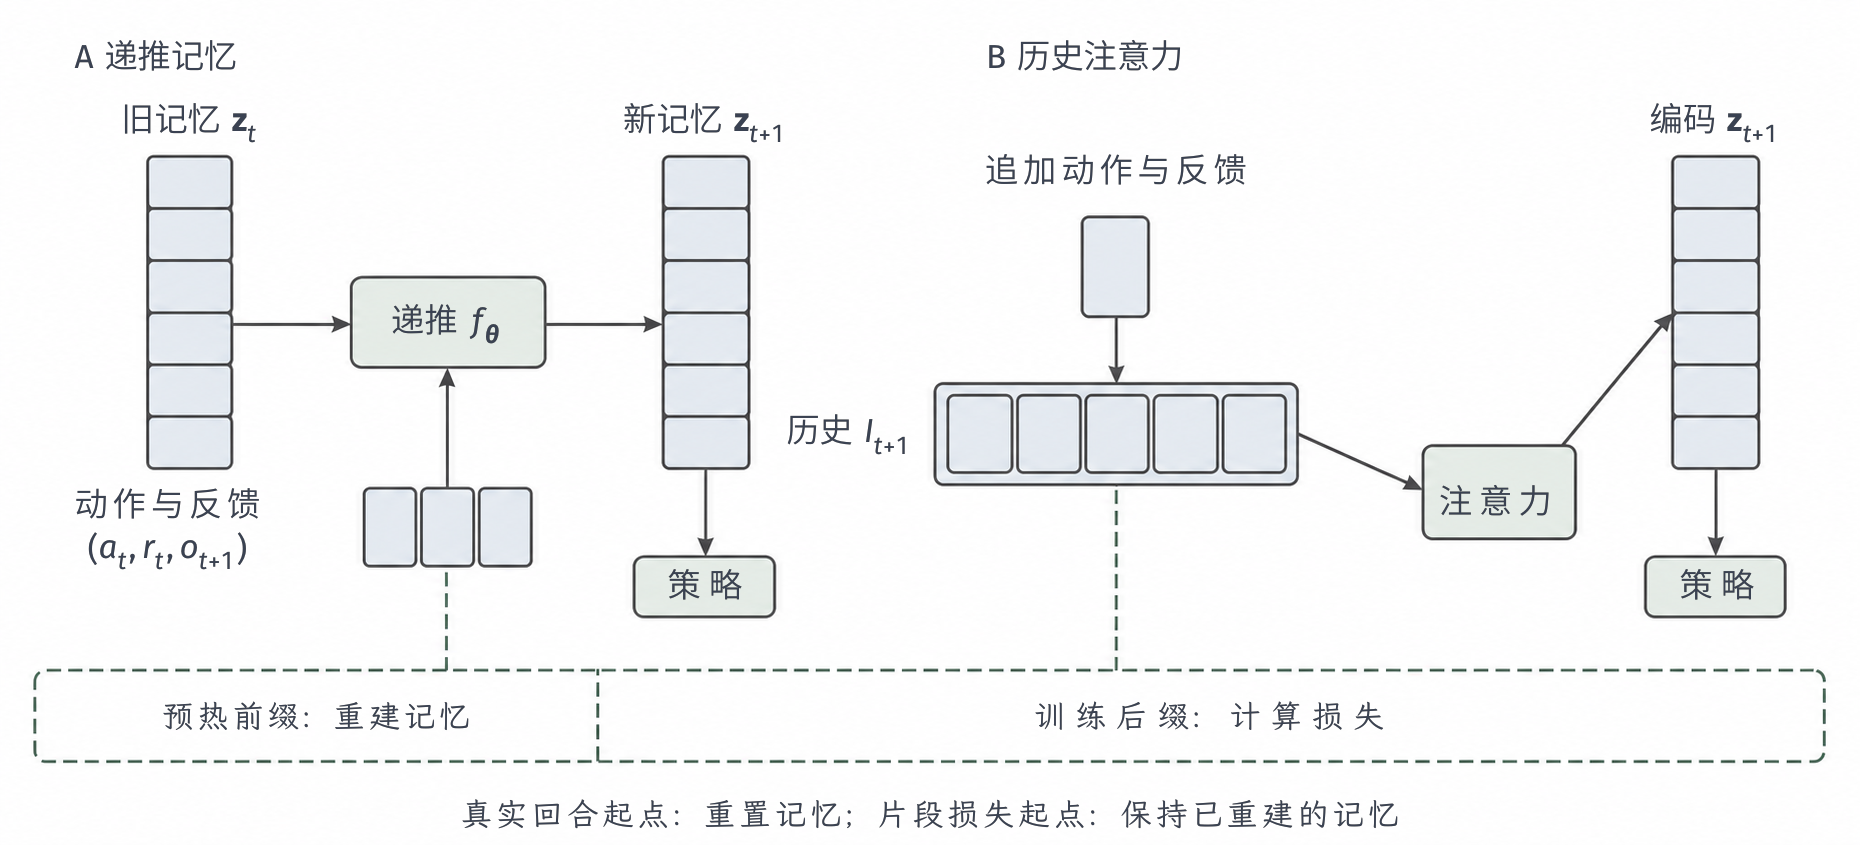
\includegraphics[width=157.400mm]{figures/10-reinforcement-learning/02-information-and-reward/generated/rl-information-memory/figure.png}
  \caption{递推记忆与历史注意力所用的交互记录及表示更新。实线描述表示与策略的计算，虚线标出训练片段及边界。预热前缀用于恢复损失起点处的记忆，不计算其训练损失。图示片段从真实回合开始；回合中部片段需用已保存状态或更早前缀初始化，片段边界本身不构成重置依据。向量与历史格数仅为示意，不规定状态维数或可见历史长度。}
  \label{fig:rl-information-memory}
\end{figure*}

训练片段与真实回合有不同边界。沿用早期提示任务，若片段从走廊中部开始，正确记忆应仍含入口提示；直接清零就使训练网络看到一段已经删掉提示的历史片段。预热让网络先读不计损失的前缀，恢复损失起点处的记忆；梯度截断则限制本次训练向多早传播。它们分别处理记忆的初始化与计算长度，不能用“只反传最近若干步”推断更早线索不重要。

\term{深度循环Q网络}（Deep Recurrent Q-Network, DRQN）将循环状态加入价值网络，使过去帧的特征可以影响当前估值。相对于堆叠有限帧，它改变了历史的保存方式，价值目标仍采用时序差分学习\scite{rl4-hausknecht2015-drqn}
序列进入重放后，还要处理参数变化导致的表示漂移和旧隐藏状态。\term{R2D2}（Recurrent Replay Distributed DQN）结合循环网络、序列重放与分布式训练，分析了这些问题。截断反向传播只限制梯度跨越多少步，并未说明更早的历史无用。burn-in即预热，先运行片段前缀恢复隐藏状态，再在后缀计算损失。也可以保存收集时的隐藏状态，减少从零启动的偏差；但网络参数更新后，保存的状态可能已不适合当前网络\scite{rl4-kapturowski2019-r2d2}

循环记忆每收到一个新记录，就把旧记忆与新取得的动作、奖励和观测变成下一记忆向量；被丢掉的细节以后通常无法重新读取。历史注意力则保留一批过去编码，计算当前表示时可以重新按相关性加权读取。前者用固定维数递推，后者用随保留窗口增长的缓存换取重读机会。两种结构都需要学习保留哪些线索，结构本身不等于已经得到精确信念。

注意力模型也可以跨片段保留过去观测、动作和奖励的编码。\term{GTrXL}（Gated Transformer-XL）在Transformer-XL中引入门控等结构调整，以适配强化学习优化。外部记忆则将历史写入独立存储，再按需读取。增加这些保存能力会带来缓存、读写和训练成本。更长的上下文或更低的预测损失，只描述保留的历史范围或训练记录上的拟合结果，尚不能证明表示满足定理~\ref{thm:rl-information-belief-sufficient}~的条件。

% Outline: 4.2.4
\subsection{基于决策状态的策略求解与动作选择}
\label{sec:rl-information-belief-control}

信念更新给出当前各状态的概率，我们还需要据此决定动作。比较时要平均可能状态的后果，并允许后续动作随新反馈改变，不能先挑一个最可能状态当成真相。\term{信念MDP}（belief MDP）把可计算的信念本身作为完全可见的决策状态。其即时奖励为
$\bar R(b,a)=\sum_s b(s)R(s,a)$，反馈概率为
$q(y\mid b,a)=\sum_{s,s'}b(s)K(s',y\mid s,a)$，状态转移通过$\tau(b,a,y)$实现。
要计算剩余时域的最优回报，可以对有限动作集$\mathsf A$中的每个动作，加上即时奖励和按反馈概率加权的继续价值，再选最大的期望回报。第~\ref{chap:rl-planning}~章的Bellman关系由此写成
\begin{equation}
  \label{eq:rl-information-belief-bellman}
  U_t^*(b)=\max_a\left\{
    \bar R(b,a)+\gamma\sum_yq(y\mid b,a)
                    U_{t+1}^*(\tau(b,a,y))\right\},
  \qquad U_H^*=0.
\end{equation}
反馈不可由控制器挑选，必须逐个更新信念、计算继续价值后按发生概率取期望。一般不能用
$U_{t+1}^*(\mathbb E[b_{t+1}])$替代$\mathbb E[U_{t+1}^*(b_{t+1})]$，因为后续动作依据实际反馈而非平均反馈选择；先平均信念会丢掉这种适应机会。

\begin{example}[Tiger中的倾听、更新与开门]
  \label{ex:rl-information-tiger}
  Tiger任务有两扇门，一侧藏着危险，另一侧可以获得奖励。隐藏状态$s\in\{L,R\}$表示危险的方向。打开安全门得10，打开危险门得$-100$，随后回合终止；倾听得$-1$，状态不变，以0.95的概率报告正确方向。令初始$b_0(L)=b_0(R)=1/2$，最多行动两次，$\gamma=0.9$，时域结束后价值为0。这些数值与两步终止规则仅用于教学，不代表所有Tiger版本。

  先比较不额外倾听的开门动作。直接打开任意一扇门，按初始危险概率加权，期望奖励都是
  $(1/2)10+(1/2)(-100)=-45$。若先倾听并得到“左侧有声”，用正确报告和错误报告的概率更新左侧危险概率，得到
  \[
    b_1(L)=\frac{0.95(1/2)}
                        {0.95(1/2)+0.05(1/2)}=0.95.
  \]
  按更新后的信念，开右门的期望奖励为$0.95(10)+0.05(-100)=4.5$，
  开左门为$0.95(-100)+0.05(10)=-94.5$；
  再次倾听只能得$-1$，之后已无动作可用，因此在这三个动作中应开右门。
  若听见右侧，按对称计算应开左门。两种反馈各以$1/2$发生，将各自的最优开门价值加权、折扣，再扣除倾听成本，初始倾听价值为
  \[
    Q_0(b_0,\text{倾听})
       =-1+0.9\bigl[(1/2)4.5+(1/2)4.5\bigr]=3.05.
  \]
  在此两步设定下，先倾听再按反馈开门的期望回报为3.05，高于直接开门的$-45$。
\end{example}

图~\ref{fig:rl-information-tiger}~显示了按反馈分开的动作比较。若固定同一个开门时刻，并把信号设为免费，最优开门收益的期望增量为$4.5-(-45)=49.5$；实际两步方案还包含倾听成本与后续折扣，不能直接使用这个增量。模型和听觉准确率虽然已知，当前危险位置仍未知，所以倾听可能有用。剩余时间不足、先验已很确定或探测成本过高时，倾听带来的开门收益增量可能不足以支付探测代价，直接开门反而更合适。

\begin{figure*}[htbp]
  \centering
  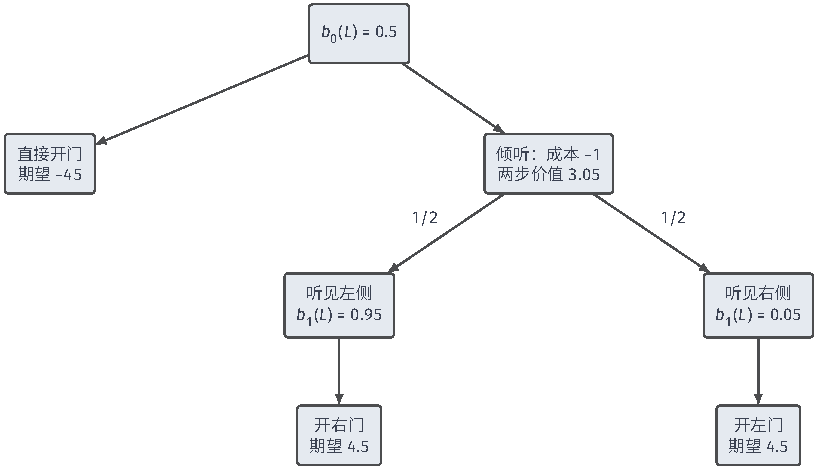
\includegraphics[width=138.511mm]{figures/10-reinforcement-learning/02-information-and-reward/tikz/rl-information-tiger.pdf}
  \caption{教学Tiger的两步决策树。$b(L)$是左门后有危险的概率。倾听反馈各以$1/2$发生，随后按新信念选择安全概率较高的门。末端标注条件期望开门奖励，根节点的3.05则计入倾听成本和折扣。}
  \label{fig:rl-information-tiger}
\end{figure*}

若只保留先验概率最大的状态，平局时任取一侧为危险，再照完全可观测解打开另一侧，预测奖励会是10，真实期望却是$-45$。这不只是平局处理的问题。将先验改为$b_0(L)=0.6$，点估计仍直接开右门，但真实期望为$0.6(10)+0.4(-100)=-34$；按0.95准确率计算两个倾听分支，先听再开的价值仍是3.05。被删除的另一侧概率影响了是否值得付费倾听，也就影响了当前动作。

\begin{example}[Tiger最后一步的回报向量]
  \label{ex:rl-information-alpha-vectors}
  沿用例~\ref{ex:rl-information-tiger}的奖励，在只剩一次行动时，按隐藏状态$(L,R)$排列，开左门、开右门和倾听对应的向量分别是$(-100,10)$、$(10,-100)$和$(-1,-1)$。令$p=b(L)$，三个信念价值分别为$10-110p$、$110p-100$和$-1$，所以$U_1^*(b)$是三者的最大值。$p=0.5$时选择倾听，价值为$-1$；$p=0.95$时选择开右门，价值为$4.5$。若只保留在$p=0.5$最优的向量，就会把$p=0.95$处的价值也估成$-1$。同一组向量在不同信念下有不同的最优者。
\end{example}

最后一步中，每个动作在两个隐藏状态下的回报构成一个向量，信念只负责给它加权。现在将这一计算推广到多步条件计划：后续动作可以随反馈分支改变，但仍能分别计算整份计划从各隐藏状态出发的期望回报。要在所有信念上比较计划，可以先保存这些回报向量，再据当前信念计算每份计划的价值。在有限非空状态集$S$、动作集$\mathsf A$、可见反馈集$\mathcal Y$及正整数时域$H$下，固定已知模型$K,R$、$0\leq\gamma\leq1$和零终端价值。把从$t$起的确定性策略写成深度至多$H-t$的条件树$\sigma$：节点规定动作，分支对应下一次可见反馈。分别从每个隐藏状态$s$开始执行这棵树，将期望折扣回报记为$\alpha_t^\sigma(s)$，这些数构成向量$\bm\alpha_t^\sigma\in\mathbb R^{|S|}$。在信念$b$下执行同一棵树的价值就是$\sum_s b(s)\alpha_t^\sigma(s)$；有限时域内这样的树只有有限棵，随机化也不能超过其中最优者。令$\bm\Lambda_t$收集这些回报向量，便有
\begin{equation}
  U_t^*(b)=\max_{\bm\alpha\in\bm\Lambda_t}\sum_{s\in S}b(s)\alpha(s).
  \label{eq:rl-information-alpha-envelope}
\end{equation}
因此，奖励最大化时的最优价值是信念单纯形上的分段线性凸函数：每棵树贡献一个线性函数，逐点取最高者形成上包络。这使连续信念上的价值比较转成有限向量比较，相关凸性背景可参考\BookChapterRef{chap:optimization}{卷1《数学准备：计算、分析与几何》中讨论最优化的章节}。

“分段线性”来自计划切换。仍令$p$为左侧危险概率，一个计划的价值是关于$p$的直线；在某个$p$范围内它最高，换到另一个范围时可能由另一条直线最高。最优值因此是这些直线的上包络，而不是把计划的回报向量先平均。一般信念有多个概率坐标，道理相同：计划固定时加权价值线性，优化时逐点选择不同计划。

完整备份须组合各反馈分支的后继树，向量数量会迅速增长。\term{点基值迭代}（point-based value iteration, PBVI）改在有限个代表信念上备份。在上述有限时域形式中，从终端零向量出发，对某个代表信念和候选动作，先在当前保留的后继向量中选出对各反馈后信念价值最高者，再把当前奖励与这些向量的模型加权折扣和合成为新向量，保留在该代表信念处价值最大的候选。这样保留下来的是定义在整个信念空间上的线性函数，而不只是各代表点的数值；但没有保留的向量仍可能在别处最优，代表信念的覆盖会影响近似质量\scite{rl4-pineau2003-pbvi}。

有限状态控制器（finite-state controller）则把过去的观测、动作和奖励压成有限个记忆节点，每个节点规定动作分布，收到反馈后按规则跳到下一节点。例如，两个节点可以分别记住左右提示，选择出口时读取节点即可。节点数限制控制器能区分多少种记忆情况，直接限制可实现的历史策略。两者分别近似价值函数和策略记忆，不能混作同一种压缩。

在特定控制问题中，估计与控制确实可以分开。线性、高斯、模型已知且没有额外约束的二次成本控制满足相应条件时，\term{线性二次高斯控制}（linear-quadratic-Gaussian control, LQG）的分离原则允许把Kalman估计的状态均值交给线性最优反馈控制器。噪声和观测机制还须与动作无关；无限时域稳定解另需可稳定性、可检测性等条件。动作若能改变观测质量，或额外奖励改变了关于隐藏状态的后验，就不能直接沿用该结论。Tiger中的倾听恰好改变后续收到的观测，因此一般POMDP没有先独立估计、再按已知状态控制的普遍保证。

模型未知时，可以把学习到的$\bm z_t$接入第~\ref{chap:rl-learning}~章的方法。循环价值学习用它构造自举目标，循环行动者—评论家用它计算动作分布和优势，潜在模型则在该表示上学习转移与奖励，用于规划或想象轨迹。这些方法学习表示、价值或动力学，但还须检查表示是否能判断未实际执行的其他动作会怎样，即是否保留了预测各候选动作后果所需的历史差别。

% Outline: 4.2.5
\subsection{近似决策状态的误差与计算边界}
\label{sec:rl-information-memory-errors}

选择历史表示时，除网络参数外，还要计算保存历史、更新表示和随后规划的成本。表~\ref{tab:rl-information-memory-cost}~按$n_S=|S|$、历史长度$t$、窗口长度$L$、单步记录的编码维度$d$、循环隐藏维度$m$和控制器节点数$n_C$列出直接实现的复杂度。这些是表中指定计算方式的成本，不是对全部模型的复杂度断言。

\begin{table*}[htbp]
  \centering
  \small
  \begin{tabularx}{\linewidth}{p{21mm}XXXX}
    \toprule
    表示 & 历史范围与存储 & 一次更新代价 & 决策或规划空间 & 充分性依据 \\
    \midrule
    完整历史 & 全部；$O(td)$ & 追加记录$O(d)$；重新读取至少随$t$增长 & 分支随时域增长的历史树 & 不主动丢弃已记录的观测、动作与奖励 \\
    精确信念 & 历史递推压缩；$O(n_S)$ & 稠密有限核$O(n_S^2)$ & $n_S-1$维单纯形；有限层可达点也可指数增长 & 已知正确模型下的充分性定理 \\
    有限窗口 & 最近$L$步；$O(Ld)$ & 缓冲追加$O(d)$，编码另计 & 窗口内记录；未必马尔可夫 & 需证明任务只依赖该窗口 \\
    有限状态控制器 & 当前节点$O(1)$；节点表另计 & 表查找可为$O(1)$ & $n_C$个记忆节点上的策略 & 策略类限制；一般非充分 \\
    学习型记忆 & 循环$O(m)$；注意力缓存随$L$增长 & 稠密循环$O(m^2+md)$；标准全窗口注意力$O(L^2m+Lm^2)$ & 学习表示上的价值或策略 & 任务与模型假设，加独立验证 \\
    \bottomrule
  \end{tabularx}
  \caption{历史与状态表示的成本及依据。注意力复杂度按宽度$m$的一层完整窗口计算，增量缓存可改变单步成本；有限状态控制器若按节点与反馈跳转，跳转表需$O(n_C^2|\mathcal Y|)$存储，若另依赖实际动作，还需乘$|\mathsf A|$。存在充分统计量不等于易于规划。}
  \label{tab:rl-information-memory-cost}
\end{table*}

例如，GTrXL中的门控与残差调整主要帮助训练保持稳定，注意力缓存和计算仍随实际保留的序列长度变化。能否较顺利地训练，与学到的表示能否充当精确决策状态，需要分别核查\scite{rl4-parisotto2020-gtrxl}

要理解压缩怎样影响动作，可以沿表示、初始化、模型和求解逐一追踪。两个历史若被编码为同一$\bm z$，却在同一动作下具有不同的反馈分布或价值，单凭$\bm z$就无法区分它们；增加训练轮数不能恢复这种表示遗漏。表示本来能保存提示，却在每个重放片段开始被清零，则是初始化错误。联合核估计不准和正确目标下优化尚未收敛，又是不同误差，各自需要对应的修正。

若要把这些误差转换为动作损失，就需要对动作价值的误差作出明确假设。固定历史$I$，在同一允许动作集上比较真实最优继续价值和近似值；假设各动作都有
$|\widehat Q(I,a)-Q^*(I,a)|\leq\delta$。分别按近似值和真实值选取最大化动作
$\hat a\in\argmax_a\widehat Q(I,a)$、$a^*\in\argmax_aQ^*(I,a)$；插入这两个动作的近似价值，真实损失满足
\[
  Q^*(I,a^*)-Q^*(I,\hat a)
  \leq
  [Q^*(I,a^*)-\widehat Q(I,a^*)]
  +[\widehat Q(I,\hat a)-Q^*(I,\hat a)]
  \leq2\delta.
\]
中间省去的差为非正，因为$\hat a$最大化近似值，即$\widehat Q(I,a^*)\leq\widehat Q(I,\hat a)$。这一界要求逐动作误差受控，平均重建损失没有直接提供该条件；没有表示误差到价值误差的论证，就不能把训练损失当作$\delta$。

例~\ref{ex:rl-information-cue}~还可以直接检验重建与控制的区别。沿用不折扣成功奖励，两个记忆节点分别保存左右提示即可达到期望值1，丢弃提示则至多达到$1/2$。即便窗口内每帧都完美重建，$1/2$的控制差距仍在。若奖励后来改为依赖另一条早期线索，仅保存$c$又可能不足，当前任务充分性不能扩展为对所有奖励目标充分。第~\ref{chap:rl-learning}~章讨论更一般的样本复杂度与函数类条件；本例先表明，表示删去的历史线索不能靠更多样本或更充分的优化补回。

% Outline: 4.3
\section{固定经验下的策略评价与选择}
\label{sec:rl-information-evaluation}

% Outline: 4.3.1
\subsection{固定经验与行为策略}
\label{sec:rl-information-logging}

下面暂时恢复完全可观测条件：每条记录都有完整状态，但学习者不能再到环境中试验。要用这些记录评价另一策略，先要弄清动作由谁、按什么概率选出。同一份状态动作表可能来自固定策略、多个策略的混合或持续更新的控制器；收集方式不同，概率校正和误差估计所用的条件也不同。

\begin{definition}[行为策略与目标策略]
  \label{def:rl-information-behavior}
  固定完全可观测环境、正整数时域$H$、$0\leq\gamma\leq1$及奖励绝对可积的回合。\term{行为策略}$\beta$生成日志动作，\term{目标策略}$\pi$是待评价或部署的决策规律。将收集的$n\geq1$个回合写为
  \[
    D=(Z_1,\ldots,Z_n),\qquad
    Z_i=(s_{i,0},a_{i,0},r_{i,0},\ldots,s_{i,H}).
  \]
  每条$Z_i$是一回合的可见记录，按采集顺序保留重复回合；状态完全可见，因而这些状态字段可以记录。理论轨迹律记为$P_{\mathcal E}^\beta$，实际记录律为$P_{\mathrm{rec}}^\beta$，两者由保留实际字段的记录映射联系。该记录组写法本身不假设各回合独立。
  有限时域评价采用价值
  $J_H(\pi)=\mathbb E_\pi[\sum_{t=0}^{H-1}\gamma^t r_t]$。
  若回合提前终止，则以吸收状态和零奖励补到$H$。$J_H$只累计有限时域，不等于无限时域的$J$；后文切换目标时将另作说明。
\end{definition}

这里有三种不同对象：环境规律规定执行动作后的真实结果，行为策略规定日志中动作怎样被选出，记录规则规定哪些字段被保存。$D$是这些机制某一次运行留下的有限材料，记录律则描述按同一协议反复采集时会出现怎样的材料。即使当前三条轨迹都相同，也不意味着其总体分布只允许这条轨迹；评价要分清样本中暂时没出现与收集机制从来不会产生。

下文$p_\sigma$表示可见记录律$P_{\mathrm{rec}}^\sigma$在离散情形的质量函数，或相对于固定共同支配测度的密度，其中$\sigma\in\{\beta,\pi\}$。支持条件针对相同记录字段；策略版本等采集元数据用于说明生成机制，不能未经说明就当成目标策略也必须复现的记录字段。

有限记录组$D$是训练或评价所用的实现样本，$P_{\mathrm{rec}}^\beta$描述这类记录的总体规律；两者都与环境及观测核所规定的生成机制不同。回合是否独立、怎样抽取转移及如何划分训练和评价记录，还须由采样协议说明。

单一马尔可夫行为策略可逐步记录$\beta(a_t\mid s_t)$。多个子策略混合时，必须区别抽取时机：每步重新按已知概率选择子策略，可以用该步混合权重加权动作概率；回合开始只抽一次，则历史会改变对所选子策略的后验，通常不能一直使用固定混合权重。后一种收集方式需要保存策略身份及相应概率并作适当的条件采样分析，或记录真正的$\beta_t(a_t\mid I_t)$；这里的历史包含行动前记录的完整状态、动作和奖励。身份字段说明了收集机制，却不能补齐某个条件层中缺失的目标动作。若策略随收集过程自适应更新，还须保存版本和选择机制。

\begin{example}[回合只抽一次控制器]
  \label{ex:rl-information-collector-mixture}
  设任务只有两步，状态只标记当前时刻。采集者在回合开始各以$1/2$概率选择“始终执行$A$”或“始终执行$B$”的控制器，于是只有$AA,BB$两种动作序列，各占$1/2$。看到首步$A$后，控制器身份已经确定，所以$\beta_1(A\mid I_1)=1$，不是$1/2$。

  对始终执行$A$的目标策略，$AA$的整轨概率比为$1/(1/2)=2$。若每步都误用固定混合概率$1/2$，就得到错误权重4。令首步奖励为0，第二步$A$得1、$B$得0，$\gamma=0.9$；正确的重加权期望为$(1/2)\times2\times0.9=0.9$，错误权重则给出1.8。回合混合与逐步混合不能只凭相同的起始权重互换。
\end{example}

动作概率描述采集者如何选动作，不是描述环境怎样给奖励。前面的回合混合例中，第一次动作揭示了本回合是哪一个控制器，所以第二次动作概率随已知历史改变；真实环境的奖励规律并未因此改变。评价必须使用实际发生的条件选择概率，才不会把同一条轨迹重复计权。

这些动作概率最好来自当时实际使用的随机化机制。机制记录正确时，概率是已知量；事后拟合的$\widehat\beta$则含有模型误差。确定性收集者没有尝试的动作，即使密度网络给出非零概率，也仍没有行为支持。表~\ref{tab:rl-information-fields}~说明哪些日志字段支撑评价中的具体计算。

\begin{table}[htbp]
  \centering
  \small
  \begin{tabularx}{\linewidth}{p{29mm}X}
    \toprule
    字段 & 支撑的计算与省略后的风险 \\
    \midrule
    状态、动作、奖励、下一状态 & 构造回报、Bellman目标及目标策略动作概率 \\
    真终止标记 & 真正终止后不再自举；终止奖励仍记在$r_t$ \\
    时间截断标记 & 区分任务结束与记录停止；持续任务截断处通常仍需继续价值 \\
    回合标识与时刻 & 恢复轨迹概率比、记忆重置和回合级划分 \\
    行为概率及策略版本 & 确定动作选择机制，区分已知概率与估计概率 \\
    初始条件、任务与目标 & 说明评价的$\mu_0$、奖励定义及任务分布是否匹配 \\
    \bottomrule
  \end{tabularx}
  \caption{完整状态日志仍需要采样元数据。有限时域的真正$H$步终止与持续任务在$H$处被时间截断，具有不同的自举目标。}
  \label{tab:rl-information-fields}
\end{table}

恢复回合边界后，还要确定统计重复的单位。独立收集的$n$个回合可以作为独立评价单位，回合内相邻转移却不能直接当作独立重复。只有一条相关长轨迹时，分块估计或相关记录的统计推断需要混合性等条件，即随时间间隔增加，相关性受到相应控制。若把相邻转移随机拆到训练与测试中，测试误差可能利用训练记录中已出现的同一条轨迹片段，也会高估独立样本数。

D4RL包含不同质量、收集者及混合任务的交互日志，因此报告时要保留具体版本、奖励定义和归一化分数的参照；仅称“专家混合日志”还不能确定实验所用的训练记录及其采集条件\scite{rl4-fu2020-d4rl}
除了日志记录组成，RL Unplugged还区分任务域与选模协议。调参是否使用在线策略测试尤其需要声明：如果依据真实环境分数选择超参数，整个选模过程就已超出纯固定经验评价\scite{rl4-gulcehre2020-unplugged}

Minari按回合提供回合记录及采集元数据接口，但具体数据集的终止、截断、环境版本和收集者说明仍须核对，存储格式并不保证行为概率可得\scite{rl4-farama-minari}
对于OGBench这样的离线目标条件强化学习基准，还要报告未记录奖励的交互轨迹组成、目标怎样选择、奖励怎样重标记以及测试目标协议。目标条件改变后，成功率不能直接横比。OGBench已有ICLR 2025正式版本；这里用它说明协议需包含哪些内容，不据其分数判断方法普遍优劣\scite{rl4-park2025-ogbench}

% Outline: 4.3.2
\subsection{策略价值的可识别性与覆盖条件}
\label{sec:rl-information-coverage}

固定日志可以交给多个候选策略评价，但每个候选会使用不同的状态动作。比较分数之前，先假设能够无限重复原收集方式，检查是否仍会有不同环境给出同样日志、却赋予候选不同价值。这是\term{可识别性}（identifiability）问题：可见回合记录的总体分布能否唯一确定目标量。若不能，增加同类样本也无法只靠估计精度解决。

\begin{definition}[策略价值可识别]
  \label{def:rl-information-identifiability}
  策略价值可识别性以给定的记录生成协议、可观察字段、环境结构假设、初始分布和目标策略为条件。若所有产生相同可见回合记录总体分布的允许环境都给出相同目标策略价值，则该价值可识别。这是总体分布的性质，不说明有限样本估计已经准确。
\end{definition}

\begin{theorem}[固定经验不能识别未覆盖动作的价值]
  \label{thm:rl-information-unseen-action}
  对单状态、单步、两个动作的任务，若日志行为只执行其中一个动作，且没有将两动作奖励联系起来的结构假设，则另一动作的价值及其相对行为策略的优劣一般不可识别。
\end{theorem}

\begin{proof}
  用两个仅在未见动作上不同的环境检验定义。唯一非终止状态为$s$，执行$a_0$或$a_1$后均终止。在$M_+$与$M_-$中，$a_0$的奖励都为0，$a_1$的奖励分别为$+1$和$-1$；两环境的行为均为$\beta(a_0\mid s)=1$。

  无论日志多大，其中只有$(s,a_0,0,s_{\mathrm{term}})$，所以可观测分布完全相同。但目标$\pi(a_1\mid s)=1$的价值分别是$+1$和$-1$，行为基线价值均为0。只使用日志的程序收到相同的有限日志记录组，在相同算法随机化规律下得到的估计或策略分布也相同，无法在两个环境中都正确确定目标价值或排序。因此，按定义，这两项结论都不可识别。
\end{proof}

这个反例中的障碍不是样本太少，而是收集规则永远不查$a_1$。如果不断重复同一规则，仍会得到完全相同的零奖励记录；在两个环境中，程序接收的证据始终一样。可识别性先检查这种“总体规律也不能区分”的缺口。只有通过这个检查，增加样本以提高估计精度才可能解决剩余困难。

给$a_1$产生数值预测还不够。神经网络可以外推，结构化动力学也可以用$a_0$的转移记录推断$a_1$的后果，但需要可核验的正确性假设说明两动作怎样联系，才可能排除上述一个环境。网络能表达这种联系，不表示日志已经证明它成立。

为检查哪些候选避开了这一缺口，可以比较候选诱导的轨迹分布和行为分布。候选可能使用而行为绝不产生的轨迹，无法通过日志重加权补出；即使没有这种绝对缺口，也要考察候选是否把大量概率放在日志极少涉及的区域。

\begin{definition}[支持、集中程度与部分覆盖]
  \label{def:rl-information-support}
  在相同可见记录空间上，目标支持条件为$P_{\mathrm{rec}}^\pi\ll P_{\mathrm{rec}}^\beta$：行为记录律赋予零概率的事件，目标记录律也赋予零概率。在共同环境核的有限模型中，目标可达历史上的每个目标动作都须有行为支持。

  若将评价改为无限时域折扣占用而非有限整条轨迹，则用前文归一化的$d^\pi(s,a)$表示目标访问概率，以$\nu(s,a)$表示训练转移记录的归一化采样分布。集中程度系数衡量目标访问相对训练记录采样可能集中到多大程度，用本质上确界记录占用比的上界而非平均大小，即取遍$\nu$支持中的状态动作、忽略$\nu$零测集。其定义为
  \[
    C_\pi=\operatorname*{ess\,sup}_{(s,a)\sim\nu}
               \frac{d^\pi(s,a)}{\nu(s,a)},
  \]
  并要求$d^\pi\ll\nu$。部分覆盖表示上述条件仅在某些策略或状态动作区域成立。可达性只说明某动作序列在环境中可能到达一处，不说明收集者赋予它正概率。
\end{definition}

有限状态下，可以把集中程度理解为各处访问权重比的最大值。假设某状态动作在训练记录采样分布中占$0.01$，在目标占用中占$0.5$，这一处比率就是50。训练记录覆盖区域中的小估计误差可能在目标策略的评价中占很大权重，所以不能只检查按训练记录采样分布平均的误差。若该处训练记录采样权重为0而目标为正，则不是把比率再放大一点的问题，而是没有支持。

非零支持排除了绝对缺口，却没有控制有限样本中的困难。目标经常使用的动作若只有$10^{-6}$行为概率，小日志很可能一次都未收集到；即使出现，概率校正也可能赋予很大权重。估计器不同，所需控制量可能是逐时占用比、轨迹密度比或其矩，不能把$C_\pi$作为所有分析的同一个条件。

\begin{table*}[htbp]
  \centering
  \small
  \begin{tabularx}{\linewidth}{p{26mm}XX}
    \toprule
    希望得到的结论 & 需要支持的行为范围 & 额外结构与不能省略的检查 \\
    \midrule
    给定策略评价 & 该策略的相关轨迹或占用 & 正确奖励、初始分布与行为机制；模型外推须有依据 \\
    候选排序 & 候选共同模型下的性能差 & 不一定要分别点识别两个价值；差的符号必须有证据 \\
    相对基线改进 & 候选与基线的比较行为 & 选择后仍有效的误差控制；训练记录不足处可限制回到基线 \\
    策略类中最优 & 足以排除所有有竞争力的替代行为 & 通常需更广覆盖或更强结构；高回报轨迹本身不够 \\
    \bottomrule
  \end{tabularx}
  \caption{结论越强，通常需要检查越多行为。结构假设可改变所需覆盖，但必须说明它如何排除与日志一致的不同环境。}
  \label{tab:rl-information-claims}
\end{table*}

表~\ref{tab:rl-information-claims}~将覆盖要求对应到结论强度。日志可能完整显示一条奖励为10的路径，却没尝试岔路处的另一动作；后者通向奖励11或$-100$，都可与日志相容。这些记录支持已观察路径可行，路径最优或偏离它的策略更好却没有同样依据。因此，少量高回报轨迹不能替代备选行为的覆盖。

% Outline: 4.3.3
\subsection{离线策略价值的估计}
\label{sec:rl-information-estimators}

价值可识别后，仍要由有限日志计算估计。\term{离策略评价}（off-policy evaluation, OPE）用其他行为策略收集的记录估计目标策略价值；这里还限制为不能新增交互。先固定待评价的$\pi$，假设回合独立、初始分布及联合奖励转移核$p$共同、行为动作概率已知，且$P_{\mathrm{rec}}^\pi\ll P_{\mathrm{rec}}^\beta$。沿用定理\ref{thm:rl-learning-importance-sampling}的矩条件，目标下每步奖励绝对可积。为确定日志应怎样加权，先按生成顺序展开有限时域马尔可夫策略的理论轨迹测度：
\[
  P_{\mathcal E}^\pi(\mathrm d\tau)=\mu_0(\mathrm ds_0)
       \prod_{t=0}^{H-1}
       \pi_t(\mathrm da_t\mid s_t)p(\mathrm dr_t,\mathrm ds_{t+1}\mid s_t,a_t).
\]
将$\pi$换为$\beta$得到行为轨迹测度；这一核乘积不要求状态或奖励有离散点概率。日志保留完整状态、动作与奖励时，在支持条件下计算两种记录律的Radon--Nikodym导数，共同初始核和环境核约去。对有限或可数动作，只需将沿途的目标动作概率除以行为概率并相乘：
\begin{equation}
  \label{eq:rl-information-weights}
  w_{i,0:t}=\prod_{k=0}^{t}
       \frac{\pi_k(a_{i,k}\mid s_{i,k})}
            {\beta_k(a_{i,k}\mid s_{i,k})}.
\end{equation}
连续动作须将每步概率比改为相应条件动作核的Radon--Nikodym导数，并核对其存在条件。这一比率把行为日志中的期望转换为目标策略下的期望，复用了第~\ref{chap:rl-learning}~章的换测度关系。初始分布若改变却未校正，或行为实际依据了未记录的观测或状态，便不能按上式消去相应因子。更一般地，当目标记录律相对行为记录律绝对连续、待求回报可积时，密度比把行为期望改写为目标期望；它只建立积分恒等式，有限方差还需二阶矩等条件。这里将该结论用于比较同一环境中两种策略的回报，可参考\BookChapterRef{chap:random-sequences-and-processes}{卷2《数学准备：概率、因果与决策》的“随机序列与随机过程”章}。

这项校正可以回接前章的一步直觉：行为以$1/2$概率选择某动作，目标以$3/4$选择它，记录该动作的样本就乘$1.5$；另一动作乘$0.5$。权重调整的是这条记录在目标评价中应占的份额，奖励数值本身不变。整条轨迹需要逐步概率比相乘，因为前面动作已经影响了后面能取得哪些状态和奖励；逐奖励评价则只乘到这项奖励产生时。

令$G_i=\sum_{t=0}^{H-1}\gamma^t r_{i,t}$。可以将每条完整回报乘以轨迹比，再对独立回合取平均；也可以对每个奖励只校正此前的动作，随后累计和平均。普通轨迹重要性采样与逐决策形式分别为
\begin{align}
  \label{eq:rl-information-is}
  \widehat J_{\mathrm{IS}}
    &=\frac1n\sum_iw_{i,0:H-1}G_i,\nonumber\\
  \widehat J_{\mathrm{PDIS}}
    &=\frac1n\sum_i\sum_{t=0}^{H-1}
                      \gamma^t w_{i,0:t}r_{i,t}.
\end{align}
奖励$r_t$在$a_t$执行后产生，校正其分布须包括$a_t$，无需包括之后的动作。截到该奖励的前缀密度比正是$w_{i,0:t}$，由此得到逐决策形式；不必另外要求目标概率为0的行为历史上后续权重条件均值为1。概率正确、支持和上述矩条件成立时，两式都无偏，但相乘的权重可能随时域快速增大。

\begin{example}[三条两步轨迹的概率校正]
  \label{ex:rl-information-ope-data}
  为核算概率校正，给定一个教学MDP：从$s_0$出发，任意动作都到$s_1$，再行动一步终止。两个时刻均可选$A,B$，奖励为$r_0(A)=1$、$r_0(B)=0$、$r_1(A)=2$、$r_1(B)=0$，奖励与转移都确定，$\gamma=0.9$。行为每步均匀选择，目标每步以$3/4$概率选择$A$。对每步目标奖励取期望再折扣，真实价值为
  $J_2(\pi)=3/4+0.9(2\times3/4)=2.1$。

  假设独立收集到$AA,BA,BB$三条轨迹。按上述动作概率计算前缀比和回报，得到
  \[
  \begin{array}{c|rrrr}
    \text{轨迹}&G_i&w_{i,0:0}&w_{i,0:1}
                    &\sum_t\gamma^t w_{i,0:t}r_{i,t}\\
    \hline
    AA&2.8&1.5&2.25&5.55\\
    BA&1.8&0.5&0.75&1.35\\
    BB&0&0.5&0.25&0
  \end{array}
  \]
  先乘完整轨迹比再平均，普通IS为$(2.25\times2.8+0.75\times1.8)/3=2.55$；
  逐奖励使用前缀比，逐决策IS为$(5.55+1.35)/3=2.3$。本批样本的两个估计都偏离2.1；无偏性说的是反复收集整批日志后的估计期望，不保证每批数值准确。
\end{example}

轨迹权重过大时，可以改动汇总方式以减轻少数样本的影响，但也会改变统计性质。自归一化估计用
$\widehat J_{\mathrm{SN}}=\sum_iw_iG_i/\sum_iw_i$，
用总权重而非$n$归一化，要求分母非零；截断估计则预先选择正阈值$c$，限制每条权重不超过$c$：
$\widehat J_{\mathrm{clip}}=n^{-1}\sum_i\min(w_i,c)G_i$。
例~\ref{ex:rl-information-ope-data}~取$w_i=w_{i,0:1}$时，
自归一化结果为$7.65/3.25\approx2.3538$；取$c=1$的未归一化截断结果为
$(2.8+0.75\times1.8)/3\approx1.3833$。前者使用随机分母，后者修改精确换测度权重，一般都会引入有限样本偏差。以拟合行为概率替代已知概率，也改变无偏性条件。

有效样本量（effective sample size, ESS）用$(\sum_iw_i)^2/\sum_iw_i^2$诊断权重集中程度。若$n$条权重都相同，这个值为$n$；若只有一条权重非零，就为1。上例权重$(2.25,0.75,0.25)$给$3.25^2/(2.25^2+0.75^2+0.25^2)\approx1.857$，说明三条记录的贡献并不均衡。这不是重新获得了1.857条独立轨迹，也没有检验奖励和行为模型是否正确，因此不能单独证明价值估计可靠。

重要性估计直接重加权已观察的回报，另一条路线则先学习目标策略的动作价值。困难是日志没有附带正确的$Q^\pi$标签。Bellman关系允许从末步开始构造标签：末步只需已观察奖励，前一步则用奖励加上已经拟合的继续价值。目标策略固定时，继续动作应按它的概率平均；取最大值会把评价问题改成控制问题。下面的拟合Q评价正是把这一反向计算交给回归器。

若日志能支持目标继续动作，也可以不乘整条轨迹的概率比，改为拟合目标策略的Bellman关系。\term{拟合Q评价}（fitted Q evaluation, FQE）固定$\pi$，用记录奖励与下一步目标价值构造回归目标，因此只评价、不取动作最大值。有限时域中令$\widehat Q_H=0$，从末步向前更新。时刻$t$在允许函数类$\mathcal F_t$中选取$f$，使训练记录上的平方残差最小；下一动作按固定$\pi_{t+1}$取期望：
\begin{equation}
  \label{eq:rl-information-fqe}
  \widehat Q_t
  \in\argmin_{f\in\mathcal F_t}
    \sum_{i}
    \left[
      f(s_{i,t},a_{i,t})
      -r_{i,t}
      -\gamma\mathbb E_{a'\sim\pi_{t+1}(\cdot\mid s_{i,t+1})}
                       \widehat Q_{t+1}(s_{i,t+1},a')
    \right]^2.
\end{equation}
其中$\mathcal F_t$限定时刻$t$可拟合的价值函数。末步$t=H-1$的继续价值直接为0，无需定义终点策略。若改为无限折扣任务，则用时间不变的函数类反复回归，以上一轮$\widehat Q^{(k)}$构造目标，得到$\widehat Q^{(k+1)}$。两种形式都在真终止处屏蔽后续项。回归后，对初始状态及目标初始动作取期望，有限时域得到$\widehat J_H(\pi)=\mathbb E_{s_0\sim\mu_0,a_0\sim\pi_0}\widehat Q_0(s_0,a_0)$；初始分布未知时，需要相应初态样本。每轮拟合要遍历训练记录或从中抽样、计算目标动作期望并求解回归，非线性函数类还会产生优化误差。小训练平方误差仅说明训练记录上的拟合，有限样本价值界另需函数类、Bellman逼近和覆盖条件\scite{rl4-le2019-fqe}

\begin{example}[在同一日志上完成FQE与DR]
  \label{ex:rl-information-fqe-dr}
  在例~\ref{ex:rl-information-ope-data}~的同三条轨迹上，每个时刻使用独立价值表。先拟合末步奖励，得到
  $\widehat Q_1(s_1,A)=2$、$\widehat Q_1(s_1,B)=0$，故
  $\widehat V_1(s_1)=0.75(2)+0.25(0)=1.5$。再将这个目标继续价值传回初始步，两个回归目标为
  \[
    \widehat Q_0(s_0,A)=1+0.9(1.5)=2.35,\qquad
    \widehat Q_0(s_0,B)=0+0.9(1.5)=1.35.
  \]
  按目标的初始动作概率加权，得到
  $\widehat J_{\mathrm{FQE}}=0.75(2.35)+0.25(1.35)=2.1$。
  本次结果精确，因为所需状态动作全已出现且后果确定；不能由此认为三条轨迹总是够用。若两时刻从零同时更新，第一轮只能拟合即时奖励，第二轮才会把1.5的继续价值传回初态。

  再将辅助预测与概率加权残差合用，观察预测不准时怎样校正。这种方法称为\term{双重稳健估计}（doubly robust estimation, DR），即权重或辅助价值有一侧正确时，在相应条件下仍可得到正确均值；具体条件将在一般公式后说明。为核算残差，事先给定不准确的辅助价值：
  $\widehat Q_1(A)=1$、$\widehat Q_1(B)=0$，
  $\widehat Q_0(A)=1.5$、$\widehat Q_0(B)=0.5$。
  对目标动作加权，得$\widehat V_1=0.75$、$\widehat V_0=1.25$。
  用实际奖励加预测继续价值减去当前预测，初始步残差$r_0+0.9\widehat V_1-\widehat Q_0$对两动作都为0.175，末步对$A$为1、对$B$为0。将这些残差按前缀比校正，加到初始预测上，三条轨迹在下面双重稳健公式中的贡献为
  \[
  \begin{aligned}
    D_{AA}&=1.25+1.5(0.175)+0.9(2.25)=3.5375,\\
    D_{BA}&=1.25+0.5(0.175)+0.9(0.75)=2.0125,\\
    D_{BB}&=1.25+0.5(0.175)=1.3375.
  \end{aligned}
  \]
  平均贡献为$2.2958$，尚有样本误差；若使用上面精确的FQE辅助值，各步残差均为0，每条轨迹都贡献2.1。
\end{example}

残差校正也可以先缩到单步教学变体。仍令行为对$A,B$各选$1/2$，目标概率为$0.75,0.25$，奖励分别为1和0。若辅助预测给$\widehat Q(A)=0.4,\widehat Q(B)=0.1$，初始预测平均为$0.325$，实际奖励相对预测的残差分别为$0.6,-0.1$。选$A$的回合贡献为$0.325+1.5(0.6)=1.225$，选$B$为$0.325+0.5(-0.1)=0.275$；按行为概率平均，得到$0.75$，恰好恢复目标回报。预测先提供一个共同起点，正确权重再补上其平均错误；有限一批记录仍会波动。

上例的DR使用有限时域逐决策形式，从预测初始价值出发，用实际反馈相对预测的Bellman残差修正。先按固定策略动作取期望，构造辅助
$\widehat V_t(s)=\mathbb E_{a\sim\pi_t}\widehat Q_t(s,a)$，
并令$\widehat V_H=0$；每个残差用截至该反馈的概率比转到目标分布，折扣累加后再平均回合贡献：
\begin{equation}
  \label{eq:rl-information-dr}
  \widehat J_{\mathrm{DR}}
  =\frac1n\sum_i\left[
    \widehat V_0(s_{i,0})
    +\sum_{t=0}^{H-1}\gamma^t w_{i,0:t}
       \bigl(r_{i,t}+\gamma\widehat V_{t+1}(s_{i,t+1})
                         -\widehat Q_t(s_{i,t},a_{i,t})\bigr)
    \right].
\end{equation}
“双重稳健”指权重或辅助价值有一侧正确时，在相应条件下仍可得到正确均值。为陈述精确无偏性，辅助函数须由与评价回合独立的辅助训练样本拟合，或交叉拟合，使评价轨迹不参与自己的辅助训练。权重正确时，残差转到目标分布，$\widehat V$和$\widehat Q$项沿时间望远镜消去，留下$J_H(\pi)$，辅助值有误也不影响等式。辅助值全部满足$\widehat Q_t=Q_t^\pi$时，给定行动前历史与当前动作，残差条件均值为0，初始价值期望则正确；有限且在反馈前确定的错误行为权重也不改变均值。两侧都错便没有这种保证，任一侧正确也不保证方差小\scite{rl4-jiang2016-dr}

辅助训练与评价分离，是为了固定一份预测以后再检验它。如果用同一个回合拟合预测并立即计算该回合残差，预测参数会随被检验的奖励一起变化，前面的固定函数期望计算就不能直接使用。交叉拟合（cross-fitting）把回合分组，每组的辅助模型由其他组拟合，再在本组计算贡献，最后合并。它重用已有回合记录但避免一条轨迹参与自己的辅助训练，仍不增加缺失动作的支持。

不使用行为概率的FQE仍需要覆盖。若上例在$s_1$只记录$B$，目标却选择$A$，$\widehat Q_1(s_1,A)$便无直接监督；其偏差$e$会以$\gamma\pi(A\mid s_1)e$进入初态目标，即使初态记录上的拟合完全正确也如此。模型评价遇到同样缺口时，传播的是奖励与转移预测误差。

轨迹比之外，还可以直接校正状态动作的分布。这里从有限时域切换到无限折扣、时间不变MDP，使用前文归一化的$d^\pi$。\term{DICE}（DIstribution Correction Estimation）类方法进行分布校正估计，不必显式拟合$\beta$，而由占用流量平衡学习
$w(s,a)=d^\pi(s,a)/\nu(s,a)$；\term{DualDICE}（Dual stationary DIstribution Correction Estimation）通过对偶优化求解这类分布校正问题\scite{rl4-nachum2019-dualdice}

\begin{example}[将分层采样校正为目标占用]
  \label{ex:rl-information-dice-flow}
  设两个状态为0、1，只有动作$a_0$，转移为$0\to1\to1$，初态为0，$\gamma=1/2$。状态0只在初始时刻访问，所以其归一化占用为$d^\pi(0,a_0)=1-\gamma=1/2$。从时刻1起，每步都处于状态1，其占用为$(1-\gamma)\sum_{t=1}^{\infty}\gamma^t=\gamma=1/2$。两处概率相加为1；后面的采样校正正是要恢复这份由实际访问路径决定的权重。

  设给定日志的转移记录已按声明的状态分层规则形成，其采样分布为$\nu(0,a_0)=0.8$、$\nu(1,a_0)=0.2$；这不是该单动作系统自然产生的折扣占用。比率为$w(0,a_0)=0.625$、$w(1,a_0)=2.5$，加权后两处质量均为$1/2$。若$R(0,a_0)=0$、$R(1,a_0)=2$，校正后的奖励均值为1，再除以$1-\gamma$得到$J=2$，与直接求和$\sum_{t\geq1}2(1/2)^t=2$一致。
\end{example}

占用校正并不是将每个状态动作看成互不相关的权重。目标策略从初态出发，经转移继续访问，各处质量必须与这条动态路径相容。上例中状态0只有起始注入，状态1不断接收从0和自身流来的质量；任意把两处占用设成别的数，一般就不再对应同一初态和动力学。下面用流量平衡约束找出相容的权重，再用它们评价奖励。

先看一个状态动作对怎样取得访问概率质量。在有限状态动作情形，目标占用满足
\[
  d^\pi(s',a')=(1-\gamma)\mu_0(s')\pi(a'\mid s')
    +\gamma\sum_{s,a}d^\pi(s,a)T(s'\mid s,a)\pi(a'\mid s').
\]
第一项是从初始分布注入的质量，第二项是此前各状态动作（包括自身）经转移和目标动作选择流入的折扣质量。把$d^\pi=\nu w$代入，对任意测试函数$f:S\times\mathsf A\to\mathbb R$加权求和，再将流入项移到左侧，就得到下面的期望关系。要求它对全部$f$成立，等价于逐个检查状态动作对的指示函数，因而给出全部流约束；$0\leq\gamma<1$时，固定初始分布、转移核与目标策略使该流方程具有唯一的折扣占用解。若有两个解，其差经状态动作转移传播并乘以$\gamma$后仍应等于自身；概率核不会增大差向量的$\ell_1$范数，而$\gamma<1$又使它收缩，因此该差只能为0。在目标占用受$\nu$支持的条件下，这些约束便确定$\nu$支持上的比率。当前测试值减去折扣后的下一测试值，其加权期望等于由初始状态与目标初始动作分布注入的概率质量；得到正确比率后再校正奖励期望：
\begin{align}
  \label{eq:rl-information-dice}
  &\mathbb E_{\nu,T,\pi}\!
       \left[w(s,a)\{f(s,a)-\gamma f(s',a')\}\right]
       =(1-\gamma)\mathbb E_{\mu_0,\pi}f(s_0,a_0),\nonumber\\
  &J(\pi)=\frac{1}{1-\gamma}\mathbb E_\nu[w(s,a)R(s,a)].
\end{align}
式中$a'\sim\pi(\cdot\mid s')$，条件正确的奖励样本可以替代奖励均值。$d^\pi$与$\nu$均归一化，而$J$是未归一化折扣回报，必须保留$(1-\gamma)^{-1}$。一般状态动作空间中，需要能辨识目标占用的足够丰富的有界测试函数类，而不是任意选取少数函数。受限函数类只能匹配其所表达的部分矩条件，不一定确定真实占用比或价值；经验求解还须分别控制函数类逼近、优化与采样误差。占用比校正仍要求目标受日志支持；省略行为拟合不会使支持外的价值可识别。

\begin{table*}[htbp]
  \centering
  \small
  \begin{tabularx}{\linewidth}{p{17mm}XXXX}
    \toprule
    估计路线 & 所需模型与日志字段 & 拟合对象 & 关键覆盖要求 & 主要误差 \\
    \midrule
    IS & 轨迹、目标与行为概率 & 可不拟合模型 & 目标轨迹相对行为绝对连续 & 乘积权重方差；概率估计偏差 \\
    模型评价 & 转移、奖励及初始条件 & $\widehat T,\widehat R$ & 目标行为后果有支持或正确结构 & 模型误设、长滚动误差 \\
    FQE & 转移、固定$\pi$、初态 & $Q^\pi$ & 目标继续动作及状态可被评价 & 回归、投影、自举传播 \\
    本节DR & IS字段和辅助价值 & $\widehat Q,\widehat V$ & 仍需目标支持；辅助拟合与评价分离 & 双方错误的交互、权重方差 \\
    DualDICE & 转移分布、初态、$\pi$ & 占用比及对偶函数 & $d^\pi\ll\nu$与可控比值 & 比率函数逼近、优化与采样误差 \\
    \bottomrule
  \end{tabularx}
  \caption{固定策略的评价路线。表中列出的是各具体形式的条件，不将某一DR或DICE变种的结论推广到全部同名方法。}
  \label{tab:rl-information-estimators}
\end{table*}

表~\ref{tab:rl-information-estimators}~按同一固定策略任务汇总了所需模型、日志字段和误差来源。评价器首先要与日志字段、支持条件相容，之后才比较方差、拟合成本和偏差控制；估计分数较高本身不是选择它的理由。

% Outline: 4.3.4
\subsection{候选策略的比较与选择}
\label{sec:rl-information-selection}

此前的估计针对固定$\pi$；若在同一日志上评价许多候选，再挑分数最高者，待报告的候选便由同一批评价记录选定了。即便每个预固定候选都无偏，最大分数也容易选中正向噪声。候选和查询次数越多，直接报告被选中的最大值越可能乐观。

候选的拟合、选择与最终报告需要区分训练样本、验证样本与测试样本。训练样本用于产生候选和拟合辅助模型，验证样本用于调参或选择候选，测试样本用于选择完成后的预定报告。各组是否独立、代表哪个总体，还须由实际划分及采样机制说明。样本少时可采用有相应依据的交叉拟合或统一误差控制；反复查看并据此选模的测试样本已经参与验证，不能再作为未参与选择的独立测试证据。所有划分仍只重用原日志，不能创造缺失支持。

对于预先固定的两个候选，可以复用同一评价轨迹计算性能差。令$\psi_\pi(Z_i)$为IS或满足相应条件的DR回合贡献，其中$\psi_\pi$是从可见回合记录到实数的统计函数，先在每个回合算$\pi_1$贡献减去$\pi_2$贡献，再平均：
\begin{equation}
  \label{eq:rl-information-paired}
  \widehat\Delta=\frac1n\sum_i[\psi_{\pi_1}(Z_i)-\psi_{\pi_2}(Z_i)].
\end{equation}
这里估计的是$\pi_1$价值减去$\pi_2$价值，真实差为正表示$\pi_1$回报更高；有限样本的估计正值还要结合误差判断。固定候选与辅助模型、使用独立同分布评价回合且贡献的二阶矩有限时，为判断差的估计波动，将相减贡献的方差展开为
\[
  \operatorname{Var}(\widehat\Delta)
  =\frac1n\left[
    \operatorname{Var}(\psi_{\pi_1}(Z))+\operatorname{Var}(\psi_{\pi_2}(Z))
    -2\operatorname{Cov}(\psi_{\pi_1}(Z),\psi_{\pi_2}(Z))\right].
\]
共享轨迹可能使两个估计同向波动，正协方差会减小差的方差，负协方差则增大它。只看两个单独价值区间是否重叠，会遗漏两种价值估计之间的协方差。

配对的收益来自共享同一份环境波动。例如某些回合整体更容易，两种策略的估计贡献可能一起升高；在同一回合先相减，这部分共同变化就可能抵消。标准误描述反复抽取同类日志时估计值的标准差，不是原始单回合奖励的标准差。下面分别给价值和性能差的标准误，说明为何应直接检查差的区间。

\begin{example}[价值区间重叠仍可比较性能差]
  \label{ex:rl-information-paired}
  构造两项价值估计5和4，各自标准误为1，两均值估计的协方差为0.98。相减得到性能差1，按方差公式计算标准误为
  $\sqrt{1+1-2(0.98)}=0.2$。另假设正态近似适用，边际95\%区间为$[3.04,6.96]$与$[2.04,5.96]$，高度重叠；配对差的95\%区间为$[0.608,1.392]$，却不包含0。这些统计量用于教学，不是实际运行实验所得。
\end{example}

图~\ref{fig:rl-information-comparison}~将单独价值与配对差的区间分开。此处价值在总体上可确定，区间来自有限样本误差；第~\ref{sec:rl-information-partial-identification}~节将改变这一条件，即使总体分布已知也可能存在多个相容价值。那里仍需比较共同模型下的差，但模型歧义与此处的采样波动是两类不确定性。

用$\widehat P_D$表示有限记录组$D$及所声明抽样权重确定的经验抽样律；只抽取状态或状态动作时，使用其相应边缘，状态边缘记为$\widehat P_D^S$。按回合均匀抽取与按单步转移均匀抽取一般不同，须随方法固定。

\begin{figure}[htbp]
  \centering
  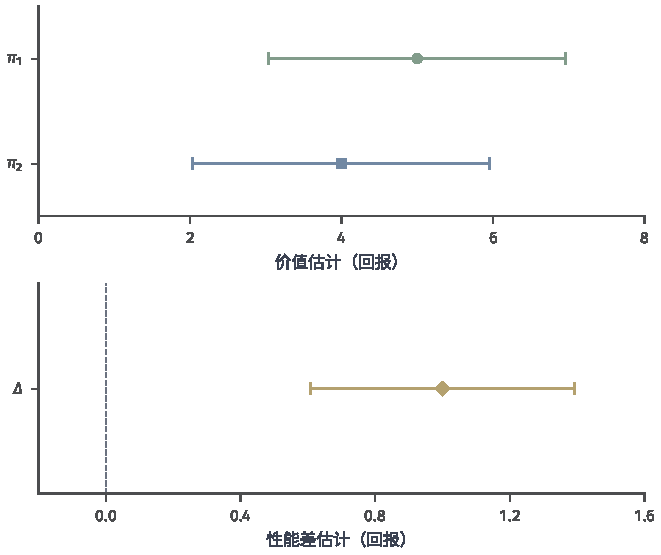
\includegraphics[width=112.000mm]{figures/10-reinforcement-learning/02-information-and-reward/matplotlib/rl-information-comparison.pdf}
  \caption{例~\ref{ex:rl-information-paired}~的教学区间。上组为两个价值的边际95\%正态近似区间，下组为共享轨迹计算的性能差区间；两组横轴各自标明量纲为回报。区间重叠与差是否包含0并非同一个判断。}
  \label{fig:rl-information-comparison}
\end{figure}

比较报告须列明候选数、产生候选所用的训练或评价记录、重复查询次数、置信水平和多重比较处理。候选集预先固定且有限时，可以分配各候选的失败概率，用并集界控制所有区间共同有效的事件；自适应增加候选不能直接沿用单候选区间。证据不足以排序时，就保留尚未排除的候选或报告无法排序。更多小数位不会增加证据。

% Outline: 4.4
\Needspace{35mm}
\section{固定经验下的策略学习与改进}
\label{sec:rl-information-offline-learning}

% Outline: 4.4.1
\subsection{策略学习的目标与数据边界}
\label{sec:rl-information-learning-boundary}

评价固定策略只检查指定行为，学习则要由日志生成新的候选。可以先以记录行为为拟合目标。\term{行为克隆}（behavioral cloning, BC）就是让策略在日志状态上给记录动作较高概率；在参数化策略类中，通过降低日志动作的平均负对数似然拟合参数：
$\min_{\bm\phi}\mathbb E_{\widehat P_D}[-\log\pi_{\bm\phi}(a\mid s)]$。
这一目标不使用奖励来重新分配概率。离线强化学习希望利用同一日志中的奖励选择行为，因此还要规定改进的比较基准。

拟合行为检查策略是否复现日志动作，提高估计回报检查学习目标是否上升。相对基线改进比较$J_H(\pi)$与$J_H(\pi_b)$，逼近最优则比较候选与允许策略类中最好的真实价值。后三者没有自动联系：优化器可能提高估计目标，却因查询日志未覆盖的动作而利用模型错误，降低真实回报。

\begin{example}[一次贪心更新利用了外推错误]
  \label{ex:rl-information-extrapolation}
  在单步教学任务中，日志只记录奖励为1的$a_0$；未记录的$a_1$真实奖励为$-10$。网络预测$\widehat Q(s,a_0)=1$、$\widehat Q(s,a_1)=5$，日志动作平方误差为0。按两个动作中的最大预测值作一次贪心更新，会选中$a_1$：估计回报从1升为5，真实回报从1降为$-10$。反复拟合原日志中的$a_0$仍不会提供$a_1$的正确后果。
\end{example}

行为克隆的目标可以用一个单状态例子看清：日志中$A$出现8次、$B$出现2次，设策略以概率$p$选$A$，平均负对数似然为$-0.8\log p-0.2\log(1-p)$，最小值在$p=0.8$。如果这两个动作的真实奖励分别为1和3，克隆策略期望奖励为$0.8(1)+0.2(3)=1.4$，而总选$B$能得3。这里两个动作都有记录，困难不是不可识别，而是拟合目标只复现动作频率，没有使用奖励来改进。

图~\ref{fig:rl-information-offline-pipeline}~把这类外推分成三个入口：策略生成新动作，价值备份查询新动作，规划器生成未观测状态动作。后续方法按限制这三个位置展开，也可组合使用。比较时保持训练记录与评价协议相同，说明优化对象、部署动作怎样产生以及额外假设；采用Transformer、扩散或流模型，并不单独说明策略是否改进。

\begin{figure*}[htbp]
  \centering
  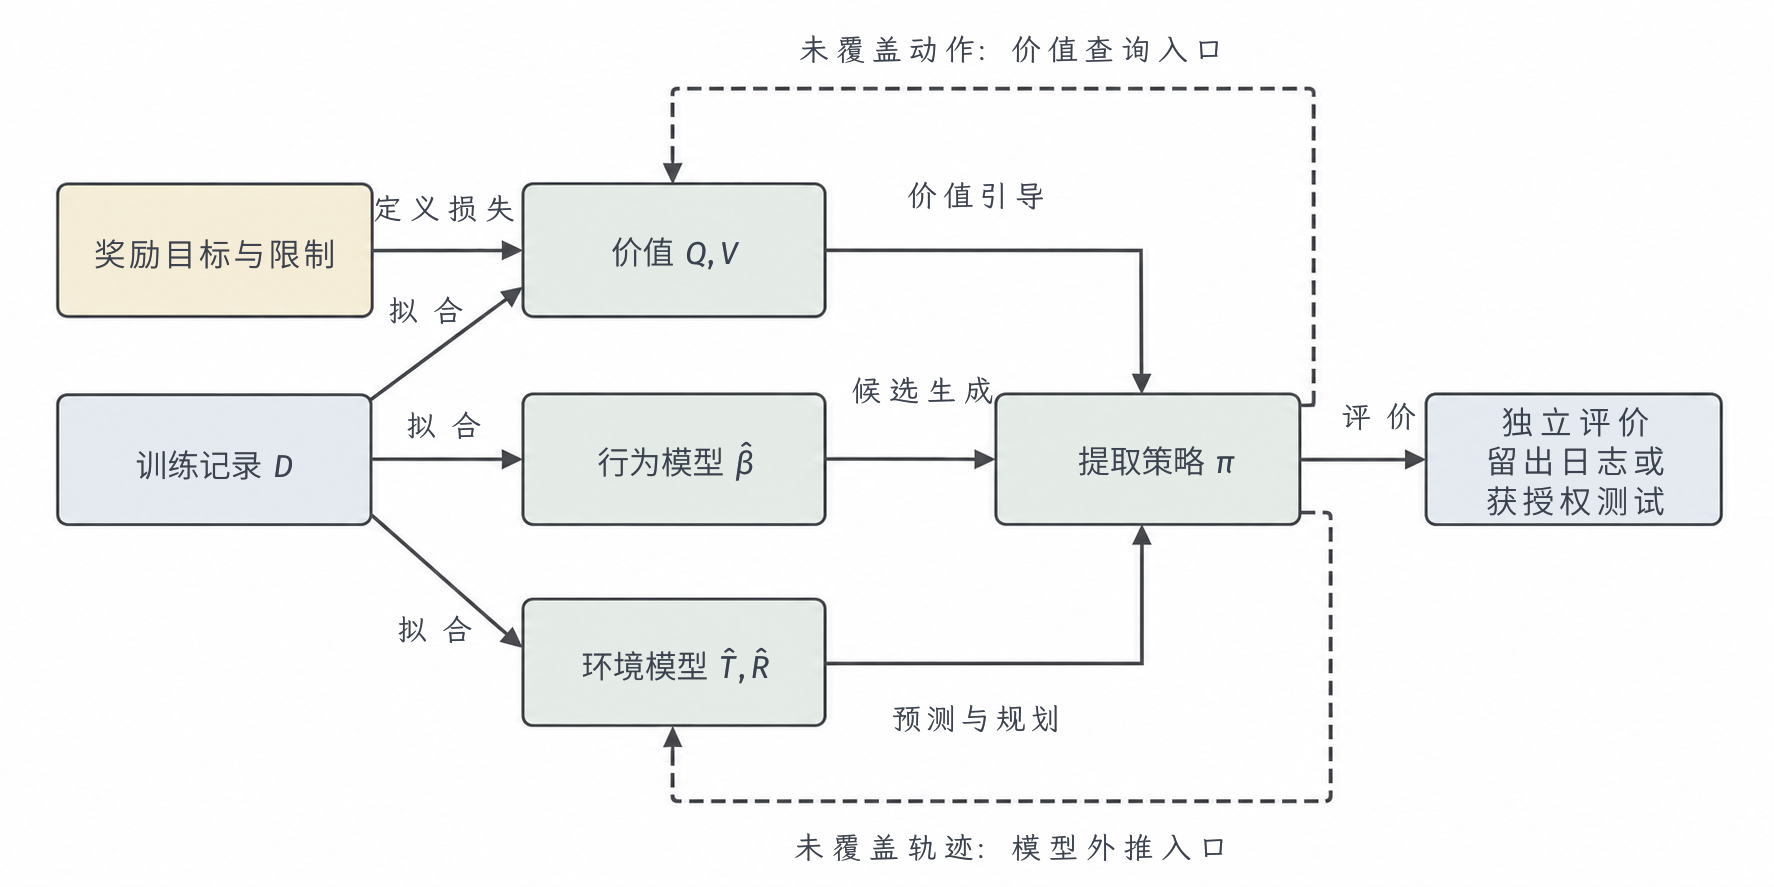
\includegraphics[width=157.400mm]{figures/10-reinforcement-learning/02-information-and-reward/generated/rl-information-offline-pipeline/figure.png}
  \caption{固定训练日志上的学习与评价。实线分别标注拟合、生成动作及评价，虚线标出外推可能进入的查询。行为约束限制动作来源，悲观价值限制对未支持动作的乐观估计，模型约束限制规划范围；任何一条学习路径仍需独立的评价证据。}
  \label{fig:rl-information-offline-pipeline}
\end{figure*}

% Outline: 4.4.2
\subsection{行为数据约束下的策略学习}
\label{sec:rl-information-behavior-constraint}

在例~\ref{ex:rl-information-extrapolation}~中，问题由策略选择未见动作触发，可以先约束候选偏离记录行为的程度。以下保持完全可观测与固定$D$，将价值目标改为无限折扣回报。TD3+BC沿用TD3的双评论家、目标网络和延迟行动者更新，在确定性行动者$f_{\bm\phi}(s)$的参数类中比较预测价值与动作平方偏差。对日志状态动作取平均，最大化价值减去偏差：
\begin{equation}
  \label{eq:rl-information-td3bc}
  \max_{\bm\phi}\ %
  \mathbb E_{(s,a)\sim\widehat P_D}
  \left[\lambda Q_{\bm\theta}(s,f_{\bm\phi}(s))
            -\lVert f_{\bm\phi}(s)-a\rVert_2^2\right].
\end{equation}
动作是向量时，范数比较各动作坐标，此处沿用动作符号$a$。为调节价值项与距离项的相对尺度，在含$N$条转移的一批训练记录上常取
$\lambda=\alpha/(\frac1N\sum_i|Q_{\bm\theta}(s_i,a_i)|)$，
其中$\alpha$控制相对强度，行动者更新时固定$\lambda$，分母为0时实现须有非零保护。按链式法则对行动者参数求梯度，可以看到两项各自推动动作的方向：
\[
  \mathbb E_{\widehat P_D}
  \left[(\nabla_{\bm\phi}f_{\bm\phi}(s))^\top
  \{\lambda\nabla_a Q_{\bm\theta}(s,a)|_{a=f_{\bm\phi}(s)}
          -2(f_{\bm\phi}(s)-a)\}\right].
\]
价值梯度推动动作朝预测价值较高处移动，距离梯度将它拉回记录动作。约束太弱可能再次利用外推，太强则接近模仿。两项的相对作用随奖励和动作尺度改变，因此比较$\alpha$必须同时给出归一化方式\scite{rl4-fujimoto2021-td3bc}

两项拉力也可手算。固定一个标量教学状态，记录动作$a=0$，暂设评论家曲线$Q(s,u)=-(u-0.6)^2$、$\lambda=1$。行动者若直接输出$u$，目标为$-(u-0.6)^2-u^2$，导数$1.2-4u$为0时得到$u=0.3$：它位于日志动作0与评论家峰值0.6之间。这只展示正则化怎样改变更新，不表示日志已证明0.3处的评论家预测正确。

平方距离还可能改变多模态行为的含义。另设左右绕障的路线参数为$-1$和1，日志各占一半，中间的0代表直行。单个确定性输出最小化平均平方偏差时得到0，却可能驶向障碍。复制均值并不等于复制两种合法路线的随机选择；这引出能够保留多个行为模式的动作生成器。

一种保留多个行为模式的办法是条件变分自编码器（conditional variational autoencoder, CVAE）。它用状态作为条件，用潜变量区分可能动作。训练时，编码器读取已记录的状态动作，将动作差别压进潜变量；解码器据状态与潜变量重构动作。部署没有待重构的真实动作，只能从先验抽潜变量，再由解码器产生候选。KL项使训练后验与采样先验保持联系，重构项让不同潜变量可以对应不同动作模式；两项都在拟合行为，不直接证明候选的真实回报。

若日志行为有多个动作模式，平方拟合可能得到模式之间日志记录稀少的均值动作。可以让行为模型生成不同模式，再在候选附近改进。\term{批量约束Q学习}（batch-constrained Q-learning, BCQ）以这种方式缩小价值筛选的动作范围。连续动作版本先在$(s,a)$记录上训练上述条件行为生成器，用$g_{\bm\omega}(s,\bm z)$表示解码器；生成候选时从规定潜变量先验采样，不再调用需要真实日志动作的编码器。随后由$\xi_{\bm\phi}(s,a)$给每个坐标加入$[-\Phi,\Phi]$内的扰动，$\Phi\geq0$，并截到合法动作域。生成$m$个候选后，仅按$Q_1$在这些修正候选中取最大值，得到执行动作：
\begin{equation}
  \label{eq:rl-information-bcq}
  a_j=g_{\bm\omega}(s,\bm z_j),\qquad
  \widetilde a_j=\operatorname{clip}_{\mathsf A}
                  (a_j+\xi_{\bm\phi}(s,a_j)),\qquad
  a_{\mathrm{exec}}\in\argmax_{\widetilde a_j,\ 1\leq j\leq m}
                  Q_1(s,\widetilde a_j).
\end{equation}

行为生成器以动作重构误差加潜变量后验相对标准先验的KL项训练。评论家备份也从下一状态生成$m$个候选，用目标网络的
$\eta\min(Q_1^-,Q_2^-)+(1-\eta)\max(Q_1^-,Q_2^-)$
评分，其中$\eta\in[0,1]$越大，越偏重两个评论家中的较小值。对候选取最高评分，构造$r_t+\gamma$倍继续价值的回归目标；真终止时后续为0。扰动网络在限幅内提高$Q_1$，目标网络缓慢更新。部署实际输出式~\eqref{eq:rl-information-bcq}~选中的动作，不是行为模型。候选数$m$为正整数，增加它会增加生成与价值计算；增大$\Phi$则放宽偏离日志的范围\scite{rl4-fujimoto2019-bcq}

例如，在一个标量教学状态下，生成器给出三个候选动作，依次为$-0.2$、$0.1$和$0.3$。扰动将它们改为$-0.15$、$0.1$和$0.25$，对应的$Q_1$评分依次为$0.4$、$0.8$和$0.6$，于是执行第二个动作$0.1$。这个筛选范围较小，却不说明三动作后果都已有充分记录：生成模型可能跨过日志缺少记录的动作区域，扰动也可能越出支持。BCQ限制的是最大化搜索范围，覆盖条件仍须检查。

其他行为正则方法也限制偏离，但度量和施加位置不同。\term{BEAR}（Bootstrapping Error Accumulation Reduction）旨在减少自举误差累积，用最大均值差异（maximum mean discrepancy, MMD）比较行动者与行为动作样本，即比较核特征中的分布均值，约束备份尽量少查询分布外动作；距离含义取决于核、样本和阈值\scite{rl4-kumar2019-bear}

这个距离先把动作映到一组用于比较分布的特征，再比较两组样本的平均特征。若只比较动作数值均值，等概率取$-1,1$与恒取0都会给均值0，无法辨别两种分布。采用更丰富的核特征，可以检查均值以外的模式差别；例如高斯核给相近动作较高相似度，远动作较低相似度。这里的核是比较动作相似性的函数，不是前面产生状态反馈的概率核。核与阈值决定能约束哪些差异，距离小仍不能证明动作后果都被日志覆盖。

\term{BRAC}（Behavior Regularized Actor Critic）考察行为正则化的行动者与评论家，比较将行为分布散度加入策略目标或价值递推的不同方式。\term{ReBRAC}（Revisited BRAC）重新考察这类设计，沿用TD3+BC，在行动者与评论家目标中分别调节行为惩罚，并检查网络、批量和归一化等实现因素。表~\ref{tab:rl-information-behavior-methods}~据此对照各自限制的位置；这些改动不增加真实转移记录\scite{rl4-wu2019-brac,rl4-tarasov2023-rebrac}

\begin{table*}[t]
  \centering
  \small
  \begin{tabularx}{\linewidth}{p{15mm}XXXX}
    \toprule
    方法 & 行为接近度 & 施加位置 & 执行动作来源 & 强度与代价 \\
    \midrule
    BEAR & 动作样本的核最大均值差异 & 行动者约束，间接限制备份 & 训练后的随机行动者；可对候选评分 & 阈值、核及拉格朗日权重；行为模型与样本比较 \\
    BRAC & 相对行为模型的KL等散度 & 策略正则，或同时进入价值递推 & 正则化行动者 & 散度权重；行为密度拟合误差 \\
    ReBRAC & 相对日志动作的平方距离 & 行动者及评论家目标的独立惩罚 & 确定性行动者 & 两处惩罚系数；日志记录的后继动作与实现配置 \\
    \bottomrule
  \end{tabularx}
  \caption{行为正则的不同位置。表中“接近”都不表示已经获得未见动作的真实后果；实际比较还需固定动作尺度、训练记录与选模预算。}
  \label{tab:rl-information-behavior-methods}
\end{table*}

还可以不用显式行为距离，改用回报条件区分日志中的动作模式。\term{Decision Transformer}是一种回报条件序列模型，将过去状态、动作与剩余回报按因果顺序编码，以监督动作预测拟合$\pi_{\bm\phi}(a_t\mid I_t,g_t)$。这里又回到有限时域，其常见条件为未折扣剩余回报$g_t=\sum_{k=t}^{H-1}r_k$，不是默认折扣$G_t$。部署由用户指定希望达到的$g_0$，每步扣去实际奖励，按$g_{t+1}=g_t-r_t$更新。训练中$g_t$描述已发生轨迹的结果，部署中它是目标愿望；条件相同不保证结果可实现\scite{rl4-chen2021-dt}

\begin{example}[回报条件不能控制外部随机结果]
  \label{ex:rl-information-return-conditioning}
  设单步教学任务的奖励与动作独立：公平硬币以$1/2$概率给1，否则给0。仅取回报1的轨迹训练条件动作模型，可以完全拟合成功轨迹记录；但部署持续输入目标1，成功概率仍为$1/2$。按结果条件化只排除了失败样本，并未得到能够改变成功概率的动作。
\end{example}

回报条件模仿由结果标签区分行为，显式距离约束则惩罚分布或动作偏离，二者目标不同。前者可以表示高回报轨迹中的动作模式，却要面对幸运随机结果、不可达目标和日志外状态。判断执行策略是否改进，仍需第~\ref{sec:rl-information-evaluation}~节的价值证据。

% Outline: 4.4.3
\subsection{价值估计与策略更新中的外推控制}
\label{sec:rl-information-pessimism}

例~\ref{ex:rl-information-extrapolation}~中的未见动作被高估，除了限制策略，也可以改变价值训练。\term{保守Q学习}（conservative Q-learning, CQL）对缺少日志记录支持的高价值增加惩罚，使策略不容易因这些预测而偏离日志\scite{rl4-kumar2020-cql}
这里保持无限折扣价值和固定训练记录，采用有限动作的一种常用形式。从所用价值函数类选择$Q$，最小化Bellman平方残差与保守正则之和。正则先对全部有限动作价值取指数、求和再取对数，使较高值有较大影响；再减去日志动作的平均价值，约束日志未覆盖的动作相对日志动作的乐观程度：
\begin{equation}
  \label{eq:rl-information-cql}
  \min_Q\
  \frac12\mathbb E_{\widehat P_D}\bigl[Q(s,a)-y(s,a,r,s')\bigr]^2
  +\alpha\mathbb E_{s\sim\widehat P_D^S}
       \left[\log\sum_{a'}e^{Q(s,a')}
                       -\mathbb E_{a\sim\widehat\beta_{D}}Q(s,a)\right].
\end{equation}
其中$\alpha\geq0$控制正则强度，$y$由固定目标网络$Q^-$构造。评价当前$\pi^{(k)}$时，按其下一动作分布取期望，可令
$y=r+\gamma\mathbb E_{a'\sim\pi^{(k)}(\cdot\mid s')}Q^-(s',a')$；
控制备份也可以使用规定的动作最大化版本，真终止处都将继续价值置0。
$\widehat\beta_{D}$是该状态下日志动作的经验分布。为检查正则修正的方向，对动作价值求导，得到
$\alpha(\operatorname{softmax}(Q)(a\mid s)-\widehat\beta_{D}(a\mid s))$；
于是无日志记录却预测很高的动作受到向下修正，日志动作得到相对支撑。连续动作不能直接枚举有限和，须按规定采样分布近似相应积分。

保守项可以看成让所有动作参与一次相对比较。Bellman回归只在日志动作上计算残差，未见动作的高预测可能没有任何修正；指数求和则会给高预测动作较大的梯度，再与日志动作频率相减。按动作价值坐标看，当某动作的softmax权重大于其日志频率时，沿保守项的负梯度更新会降低该动作的预测值。这是在控制策略容易利用的相对乐观程度，而非从未见动作获得真实负奖励标签。

沿用例~\ref{ex:rl-information-extrapolation}~的动作与日志，另设教学预测
$Q(a_0)=0,Q(a_1)=4$。未见$a_1$的正则梯度约为$0.982\alpha$，梯度下降会压低它。这解释了局部抑制机制，却不证明训练后所有$Q(s,a)$都是可信下界。CQL理论还依赖表格或特定逼近、采样误差、正则强度及策略更新条件；常用版本控制策略期望价值下界，不能扩大为每个动作的逐点下界。

也可以改变继续价值的计算，避免价值训练查询新行动者提出的日志未覆盖的动作。\term{隐式Q学习}（implicit Q-learning, IQL）从同一状态的日志动作价值中拟合偏向较高值的状态价值，再用它构造Q目标。要表达这种偏向，可用\term{期望分位数}（expectile）：以不对称权重计量高估和低估的平方误差，找出平均损失最小的位置。它不同于按概率质量切分的分位数，还考虑两侧偏差大小。对于平方可积的$X$和$\tau\in(0,1)$，比较所有实数位置$v$，定义
\begin{equation}
  \label{eq:rl-information-expectile}
  \ell_\tau(u)=|\tau-\mathbb I\{u<0\}|u^2,\qquad
  e_\tau(X)\in\argmin_v\mathbb E[\ell_\tau(X-v)].
\end{equation}
$\mathbb I$是指示函数，$u=X-v$为预测偏差。$\tau=1/2$使两侧权重相同，得到均值；$\tau>1/2$加重低估较大$X$的惩罚，使最优$v$向上移动。对离散分布求导，最优点满足
$\tau\mathbb E[(X-v)_+]=(1-\tau)\mathbb E[(v-X)_+]$。

先用一个状态的动作值观察IQL怎样改变拟合权重。我们先求上侧的状态价值$V$，再用$A(s,a)=Q(s,a)-V(s)$比较各日志动作。策略拟合时让优势较大的记录占更大权重，取$\exp(\lambda_{\mathrm{AWR}}A)$，其中$\lambda_{\mathrm{AWR}}\geq0$控制同一优势差被放大多少。它改变的是行为克隆中各记录的相对权重，后面再写成三组训练损失。

\begin{example}[三个动作的IQL更新与提取]
  \label{ex:rl-information-iql}
  在教学状态$s$，三个日志动作等频出现，目标Q值为0、1、3，取$\tau=3/4$。为找状态价值，先假设$v\in[1,3]$，将一项低估与两项高估按损失权重平衡：
  \[
    \tfrac34(3-v)=\tfrac14[(v-0)+(v-1)],
  \]
  解为$v=2$，确实落在假设区间；损失凸，故为全局最优点。对到达$s$的非终止转移，若奖励0.5、$\gamma=0.9$，继续价值便给出Q回归目标$0.5+0.9(2)=2.3$。

  提取策略时取$\lambda_{\mathrm{AWR}}=\log2$。三个优势$-2,-1,1$对应未归一化权重$1/4,1/2,2$。策略若可在所有分类分布中选择，则最大化加权对数似然等价于按等频日志动作的权重归一化，得到
  \[
    \pi(a_1\mid s)=1/11,\quad
    \pi(a_2\mid s)=2/11,\quad
    \pi(a_3\mid s)=8/11.
  \]
  若这些Q恰好等于单步真实奖励，提取策略的真实价值为$26/11$，高于等频行为的$4/3$，仍低于总选$a_3$的3。这一特殊情形也说明，拟合所得$V=2$不等于执行策略价值$26/11$。
\end{example}

在刚才的等频$0,1,3$例中，均值为$4/3$，$0.75$分位数为3，而$0.75$期望分位数为2。分位数只用两侧概率质量定位，期望分位数还平衡两侧距离，因而得到不同位置。IQL用上侧位置偏向较好的日志动作，再让策略更多拟合这些动作；随机奖励或随机后继仍由Q回归平均，不能把幸运结果也当成可选择的动作。

IQL在每个状态按日志动作的经验分布形成上述随机变量$Q(s,a)$。以下回到无限折扣价值，保持固定训练记录；$Q_{\bar{\bm\theta}}$为固定目标网络，$V_{\bm\psi}$为状态价值网络。先在各自参数类中最小化$L_V$拟合上侧位置，再最小化$L_Q$拟合奖励加继续价值，最后最小化$L_\pi$，用优势指数提高较好日志动作的拟合权重：
\begin{align}
  \label{eq:rl-information-iql}
  L_V(\bm\psi)
    &=\mathbb E_{(s,a)\sim\widehat P_D}
       \ell_\tau(Q_{\bar{\bm\theta}}(s,a)-V_{\bm\psi}(s)),\nonumber\\
  L_Q(\bm\theta)
    &=\mathbb E_{\widehat P_D}
       [Q_{\bm\theta}(s,a)-r-\gamma V_{\bm\psi}(s')]^2,\nonumber\\
  L_\pi(\bm\phi)
    &=-\mathbb E_{(s,a)\sim\widehat P_D}
       [\exp(\lambda_{\mathrm{AWR}}\widehat A(s,a))\log\pi_{\bm\phi}(a\mid s)],\\
  \widehat A(s,a)&=Q_{\bar{\bm\theta}}(s,a)-V_{\bm\psi}(s).
  \nonumber
\end{align}
每次更新将目标量固定，真终止时$V(s')=0$。$\lambda_{\mathrm{AWR}}\geq0$是逆温度，控制优势差怎样转为相对拟合权重。可先完成价值拟合再提取策略，也可交替训练，但策略梯度不反向改变价值目标。实践中还使用双Q较小值和权重截断，须报告阈值。上侧expectile施加在同状态的动作价值上，而Q平方回归仍平均奖励及随机转移，不挑选幸运反馈。原IQL用分开的$V$、$Q$目标保持了可选择动作与不可选择环境结果的区别\scite{rl4-kostrikov2022-iql}

\begin{algorithm}[固定经验上的IQL与策略提取]
  \label{alg:rl-information-iql}
  \begin{algorithmic}[1]
    \Require 固定$D$，$\gamma,\tau,\lambda_{\mathrm{AWR}}$，价值与策略更新预算，权重截断阈值
    \Ensure 可执行$\pi_{\bm\phi}$及训练、验证与最终评价记录的用途说明
    \State 初始化$Q_{\bm\theta},Q_{\bar{\bm\theta}},V_{\bm\psi},\pi_{\bm\phi}$
    \For{每次价值更新}
      \State 从$D$抽取转移批次，按$L_V$拟合日志动作Q值的expectile
      \State 按真终止标记屏蔽继续价值，构造固定目标$r+\gamma V_{\bm\psi}(s')$
      \State 按$L_Q$更新评论家，再缓慢更新目标Q参数
    \EndFor
    \For{每次策略提取更新}
      \State 固定价值网络，计算日志动作优势和截断后的指数权重
      \State 最小化加权负对数似然$L_\pi$
    \EndFor
    \State 固定提取策略，按第~\ref{sec:rl-information-evaluation}~节评价，不以$V$直接充当最终证据
  \end{algorithmic}
\end{algorithm}

算法~\ref{alg:rl-information-iql}~按给定更新预算先拟合价值，再用固定价值提取动作分布，最后将执行策略送往评价。表~\ref{tab:rl-information-extraction}~进一步对照提取方式：同一价值函数经不同动作来源形成不同策略，其逼近误差与覆盖风险也不同。

\begin{table*}[htbp]
  \centering
  \small
  \begin{tabularx}{\linewidth}{p{26mm}XXX}
    \toprule
    提取方式 & 动作来源与价值查询 & 逼近误差 & 覆盖风险 \\
    \midrule
    直接贪心 & 全动作优化或行动者提出动作；查询其Q值 & 动作优化不精确、评论家误差 & 容易主动寻找日志未覆盖的高估动作 \\
    优势加权拟合 & 用日志动作训练执行分布；训练查询日志动作的Q值 & 策略族与加权分布不匹配、优化误差 & 连续输出仍可能落在稀疏间隙 \\
    行为采样后筛选 & 生成$m$个候选，按Q取最大或重采样 & 行为生成偏差、有限$m$误差 & 生成概率非零不证明环境后果有支持 \\
    \bottomrule
  \end{tabularx}
  \caption{价值学习之后的三个动作接口。增大候选数或策略容量可能减少提取误差，也可能更充分地利用价值外推误差。}
  \label{tab:rl-information-extraction}
\end{table*}

扩散模型也可接入这些动作提取方式。

简单的单峰行动者可能难以拟合优势重加权后的多种动作模式。扩散动作模型从随机噪声开始，按学得的条件去噪步骤逐渐生成动作，借不同噪声样本保留多个模式。价值可以参与训练，使生成过程偏向高评分动作，也可以只在候选生成之后进行筛选。这两种连接改变的是梯度是否进入生成器，不能因为都生成动作就视为同一个策略更新。

\term{Diffusion-QL}（Diffusion Q-learning）将扩散动作建模与Q学习结合，拟合条件动作扩散模型，并在去噪目标外最大化生成动作的价值，让价值梯度经生成过程改变策略。行为建模与价值驱动训练由此结合，去噪步数则同时影响训练和推理成本\scite{rl4-wang2023-diffusionql}
\term{IDQL}（Implicit Diffusion Q-learning）将隐式Q学习与扩散动作模型结合，研究价值目标对应的行为重加权分布，以扩散行为模型生成候选，按评论家导出的权重重采样，或采用贪心提取变体。它试图减少简单行动者无法表示多模态隐含策略的误差；生成候选仍不提供新的环境后果证据\scite{rl4-hansenestruch2023-idql}

图~\ref{fig:rl-information-extraction}~区分价值梯度改变生成器与价值筛选已有候选。流模型也能通过可微变换把简单噪声变成动作分布，生成候选或提供动作映射；要据此说明改进，仍须接入有依据的价值加权、策略目标或规划准则。单独拟合条件生成模型没有完成这一比较步骤。

\begin{figure*}[htbp]
  \centering
  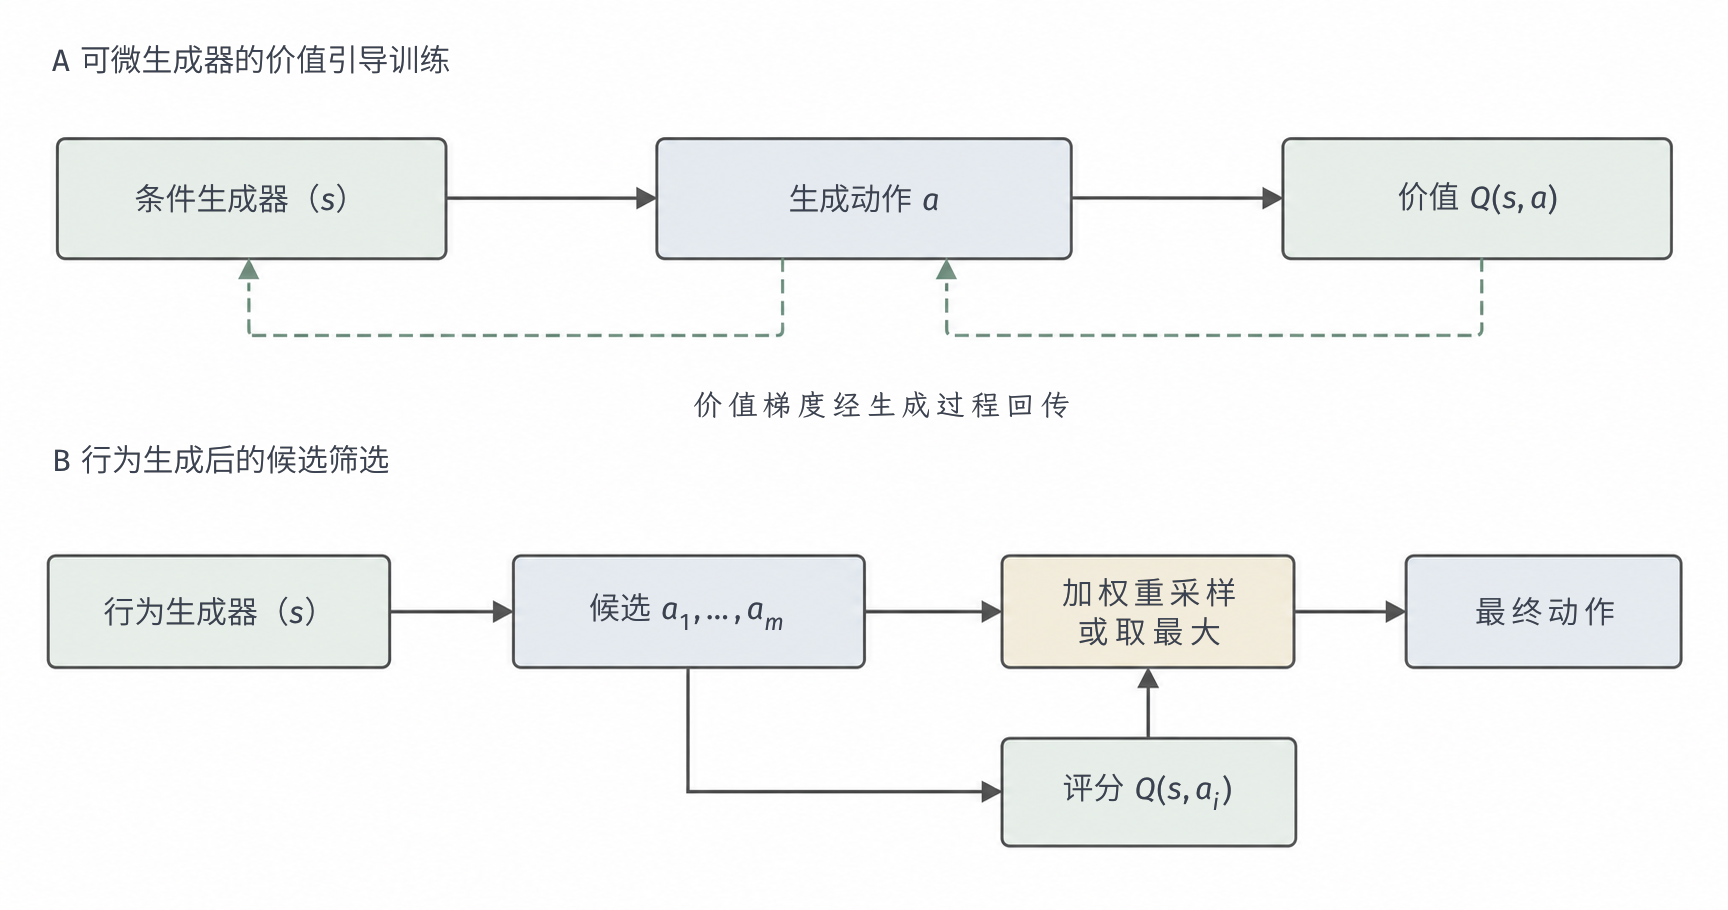
\includegraphics[width=157.400mm]{figures/10-reinforcement-learning/02-information-and-reward/generated/rl-information-extraction/figure.png}
  \caption{生成式动作的两种价值接口。实线表示动作生成、价值评价与候选选择。A的虚线将动作价值梯度经生成动作和可微生成过程回传到生成器；B把候选和对应评分分别送入筛选，再给出最终动作。A改变生成器，B筛选已有候选，两者属于不同的策略构造接口。}
  \label{fig:rl-information-extraction}
\end{figure*}

动作还可以组合为序列。近期\term{DEAS}（DEtached value learning with Action Sequence）研究动作序列上的价值学习，将其与显式行动者分离，以减轻动作块评价的过估计；其ICLR 2026正式版本研究长时程离线任务与动作序列模型。动作块减少显式选择次数，却扩大了组合动作空间；固定长度序列也不等于能够中途依反馈行动的Option，更不说明日志覆盖全部动作块。这里只将DEAS作为该接口的近期研究，基准表现不构成普遍最优性结论\scite{rl4-kim2026-deas}

% Outline: 4.4.4
\subsection{学习模型上的规划与策略优化}
\label{sec:rl-information-model-learning}

第~\ref{chap:rl-learning}~章允许新交互，因此规划器查询到模型的可疑预测后，还可采样校正；固定经验下无法这样验证。我们仍可从日志拟合$\widehat R(s,a)$和$\widehat T(s'\mid s,a)$，并计算不确定性分数$u(s,a)$。留出转移记录能检查其覆盖区域中的部分预测误差；日志未覆盖状态动作的真实后果却不能仅由小误差、小集成分歧或高似然证明。

\term{MOPO}（Model-based Offline Policy Optimization）在学习模型上进行离线策略优化，模型滚动时扣除不确定性惩罚：从日志状态出发，按当前策略在$\widehat T$中生成有限长度轨迹，以
$\widetilde R=\widehat R-\lambda u$作为模拟奖励，再混合真实与模拟转移更新策略并重复这一过程。模型只由真实$D$拟合，模拟转移保留来源标识。滚动长度控制误差可累积的范围，$\lambda$调节不确定区域的惩罚\scite{rl4-yu2020-mopo}

惩罚有两种不同含义。若$u$只是模型成员的分歧，扣去$\lambda u$会降低分歧大区域的评分，但成员也可能一致地错；这只是一项偏好调整。若能证明惩罚至少覆盖相关奖励和下一价值预测误差，扣除后才有依据称为保守下界。接下来把误差逐项写出来，说明这两个意义之间需要哪一步论证。

要把惩罚后的回报解释为真实价值下界，需要知道它扣除的量能否覆盖模型误差。固定$\pi$和无限折扣目标，令$\widehat d^\pi$为$\widehat T$下的归一化占用。为计算真实价值减去模型价值，将两个Bellman方程相减，并按模型轨迹的访问概率累积，得到
\begin{equation}
  \label{eq:rl-information-model-telescoping}
  J_M(\pi)-J_{\widehat M}(\pi)
  =\frac1{1-\gamma}\mathbb E_{\widehat d^\pi}
       \left[R-\widehat R
                  +\gamma(T-\widehat T)V_M^\pi\right].
\end{equation}
这里$(T-\widehat T)V$是两核给出的下一价值期望之差。共同$\mu_0$和有界价值使折扣尾项消失；占用已归一化，故保留$1/(1-\gamma)$。若在该策略访问区域内，
$|R-\widehat R|\leq u_R$且
$|(T-\widehat T)V_M^\pi|\leq u_T$，
则每处误差项不低于$-u_R-\gamma u_T$。按同一非负占用分布平均，得到扣除奖励与转移价值误差上界后的保守回报：
\[
  J_M(\pi)\geq
    \frac1{1-\gamma}\mathbb E_{\widehat d^\pi}
       [\widehat R-u_R-\gamma u_T].
\]
因此，$\lambda u$只有与实际误差上界建立联系，才具有上述下界含义。用它选择策略时，条件还须同时覆盖参与选择的候选，不能沿用单个预固定策略的界。所有集成模型也可能一致地学错；没有覆盖或正确结构支撑时，模型分歧仍只是启发式诊断。

除惩罚奖励外，\term{MOReL}（Model-Based Offline Reinforcement Learning）也是基于模型的离线强化学习方法，在不可信状态动作处转入低回报吸收状态，使规划器少离开可信区域\scite{rl4-kidambi2020-morel}
\term{COMBO}（Conservative Offline Model-Based Policy Optimization）在学习模型上进行保守离线策略优化，对模型滚动状态动作施加保守价值正则，不必先构造同一种显式不确定性分数\scite{rl4-yu2021-combo}
两者都仍需要真实交互记录和各自保证中的模型误差条件。表~\ref{tab:rl-information-model-methods}~在相同日志缺口下比较这些选择：未见动作若实际很好，保守限制会放弃可实现回报；若实际很差，限制可能阻止规划器利用错误预测。

\begin{table*}[t]
  \centering
  \small
  \begin{tabularx}{\linewidth}{p{17mm}XXXX}
    \toprule
    方法 & 限制位置 & 候选轨迹来源 & 真实交互记录依赖 & 保守程度与代价 \\
    \midrule
    MOPO & 模型奖励减去误差代理惩罚 & 日志状态出发的短模型滚动 & 动力学拟合及误差校准 & 惩罚系数、滚动长度；可能拒绝高回报稀疏区域 \\
    MOReL & 不可信区域进入低回报吸收态 & 悲观模型中的规划或学习 & 可信区域判定与模型置信 & 阈值与吸收惩罚；错误拒绝会缩小可达策略类 \\
    COMBO & 真实交互与模型生成转移上的保守价值正则 & 学习模型中的策略滚动 & 模型拟合及日志动作的价值支撑 & 正则及混合比例；过强会压低真实可行动作 \\
    \bottomrule
  \end{tabularx}
  \caption{模型法限制外推的三个位置。比较成立的前提是任务、日志、模型容量与查询预算相同；减少显式不确定性估计不等于不再需要误差依据。}
  \label{tab:rl-information-model-methods}
\end{table*}

另一种模型使用方式是直接生成整段轨迹。\term{Trajectory Transformer}是一种轨迹序列预测模型，自回归地预测状态、动作与奖励序列，规划时用束搜索保留高评分候选，再执行选中轨迹的首个动作；收到真实观测后重新搜索。改进还取决于搜索评分与候选可行性，不能仅由下一token预测损失推出。
\term{Diffuser}用扩散模型进行轨迹规划，按当前状态等条件，通过回报引导的扩散采样形成计划，也可执行首个动作后滚动重规划。前者搜索自回归候选，后者引导去噪生成计划，但两者轨迹都是模型预测，没有增加观测经验\scite{rl4-janner2021-trajectory,rl4-janner2022-diffuser}

部署接收反馈并重规划，不说明训练期间有在线调参权限。若为选超参数反复在真实环境执行计划，这些查询须计入第~\ref{sec:rl-information-limited-interaction}~节的新增预算。搜索与模型滚动的通用计算见第~\ref{chap:rl-planning}、\ref{chap:rl-learning}~章；固定日志下，规划器仍不能自行验证日志未覆盖区域的模型预测。

% Outline: 4.4.5
\subsection{策略改进的保证与比较}
\label{sec:rl-information-improvement}

前述三类限制都产生了候选，但候选价值超过估计基线还不等于真实改进。需要先规定比较哪些策略，以及估计误差能否同时约束它们。下面固定候选集合与基线，用共同误差事件计算选择后策略最多可能损失多少回报，不依赖特定网络或优化器。

\begin{theorem}[共同误差事件上的基线性能控制]
  \label{thm:rl-information-improvement}
  固定任务、初始分布、时域口径、非空候选策略集合$\Pi$及基线$\pi_b$，并假设所涉真实价值与估计值均为有限实数。给定$\varepsilon\geq0$；在日志与算法随机性所定义的概率空间上，若可测事件$C_{\mathrm{conf}}$中每个
  $\pi\in\Pi\cup\{\pi_b\}$均满足
  $|\widehat J(\pi)-J(\pi)|\leq\varepsilon$，且从$\Pi$中选出的可测策略$\widehat\pi$满足
  $\widehat J(\widehat\pi)\geq\widehat J(\pi_b)$，则该事件中真实价值满足
  \[
    J(\widehat\pi)\geq J(\pi_b)-2\varepsilon.
  \]
  若另给定$\delta\in[0,1]$且$\mathbb P(C_{\mathrm{conf}})\geq1-\delta$，结论也以至少$1-\delta$的概率成立。
\end{theorem}

\begin{proof}
  为把估计上的选择规则转为真实价值比较，在共同事件内插入候选和基线的估计值：
  \[
  \begin{aligned}
    J(\widehat\pi)
    &\geq\widehat J(\widehat\pi)-\varepsilon\\
    &\geq\widehat J(\pi_b)-\varepsilon\\
    &\geq J(\pi_b)-2\varepsilon.
  \end{aligned}
  \]
  第一、三步分别使用$\widehat\pi$与$\pi_b$的共同误差界，第二步使用选择规则。事件$C_{\mathrm{conf}}$发生时这条链必成立，故结论概率不低于$\mathbb P(C_{\mathrm{conf}})$。
\end{proof}

这一界允许真实回报比基线低$2\varepsilon$，并不保证严格提高。将选择阈值提高到
$\widehat J(\widehat\pi)-\widehat J(\pi_b)>2\varepsilon$，同样推导才给出严格正的真实增量。共同事件是关键条件：预固定单策略的95\%区间不能直接约束从许多候选中选出的最好者；候选集若由评价记录生成，还须处理适应性。

两侧误差可以先用数值检查。若候选估计价值为0.8、基线为0.7，二者误差各不超过0.1，允许的真实值仍包括候选0.7、基线0.8；估计领先0.1不能保证真实领先。候选估计领先必须严格超过0.2，才能排除两侧误差同时取最不利方向。这说明阈值不是任意保守系数，而来自比较时两份估计都可能出错。

共同误差界也可以进入候选策略的构造。若估计备份高的动作恰好也是日志稀少的动作，直接贪心可能选中正向估计误差；可以先扣除覆盖该误差的不确定性半径，再比较动作。\term{悲观值迭代}（pessimistic value iteration, PEVI）按这个思路反向规划。

一个单步教学例能显示扣除半径的作用。两个动作的奖励均值估计为$(0.6,0.8)$，假设已证有效的半径为$(0.05,0.4)$，悲观值就是$(0.55,0.4)$，于是选择第一个动作。若真实均值为$(0.58,0.4)$，两项绝对误差均在给定半径内；直接按估计贪心会选第二个动作，损失$0.18$，悲观选择则没有损失。此时最优动作半径给出的界为$2(0.05)=0.1$。这些构造值不提供半径有效性的统计证明；实际还须根据采集协议、模型或函数类证明共同事件。最优策略访问处缺少证据时，半径仍可很大，界也会很宽。表格或线性模型中成立的半径构造，不能仅凭同样使用悲观惩罚就移给深度CQL。

为明确其保证，改用完全可观测、时间齐次的有限MDP：$S,\mathsf A$有限非空，$H$为正整数，$t=0,\ldots,H-1$，$0\leq r_t\leq1$，不折扣，终端价值为0。日志$D$来自该MDP并保留完整转移字段；采集协议及算法随机性规定下述概率空间。真实备份作用于$v:S\to\mathbb R$：
\[
  (\mathcal B_t v)(s,a)
    =R(s,a)+\sum_{s'}T(s'\mid s,a)v(s').
\]

这项反向规划与在线探索的乐观备份方向相反。在线时，可以暂按较高价值尝试不确定动作，再用新经验修正；固定日志无法补试，因而先扣除误差半径，避免把未证实的好处当成行动依据。没有样本的动作需要用完整可能回报范围给大半径，不能因无法计算样本误差就设为0。下面的更新把固定日志不能补采记录的限制转成可计算目标。

从$\widehat V_H=0$按$t=H-1,\ldots,0$反向计算时，由同一训练日志$D$构造备份估计$\widehat m_t(s,a)$和非负半径$u_t(s,a)$。表格实现可以对相应$(s,a)$转移记录中的$r+\widehat V_{t+1}(s')$求平均，估计一次动作的奖励加继续价值；没有记录时，可例如约定$\widehat m_t(s,a)=0$、$u_t(s,a)=H-t$，用完整剩余回报范围覆盖未知备份，不能把缺失当作零误差。需要一个概率至少为$1-\delta$的共同可测事件$C_{\mathrm{pess}}$，其中$0<\delta<1$，使下式对所有$s\in S$、$a\in\mathsf A$及$t=0,\ldots,H-1$同时成立：
\begin{equation}
  \left|\widehat m_t(s,a)
       -(\mathcal B_t\widehat V_{t+1})(s,a)\right|
       \leq u_t(s,a).
  \label{eq:rl-information-pevi-confidence}
\end{equation}
这里$\widehat V_{t+1}$本身由$D$递归生成，误差界必须涵盖这一依赖；只对事先固定的$v$给出逐点置信区间还不够。减去半径后，再把数值截到剩余回报的允许范围：
\begin{equation}
  \begin{aligned}
    \widehat Q_t(s,a)
      &=\min\{H-t,\max\{0,\widehat m_t(s,a)-u_t(s,a)\}\},\\
    \widehat V_t(s)&=\max_{a\in\mathsf A}\widehat Q_t(s,a).
  \end{aligned}
  \label{eq:rl-information-pevi-backup}
\end{equation}
令$\widehat\pi_t(\cdot\mid s)$只给最大化动作分配概率，即每一步都对$\widehat Q_t$精确贪心。双侧误差界及截断使残差$(\mathcal B_t\widehat V_{t+1})(s,a)-\widehat Q_t(s,a)$位于$[0,2u_t(s,a)]$。若$V_t^\pi(s)$表示该有限MDP中从$s$起的剩余期望回报，$\pi^*$为全部时变马尔可夫策略中的最优者，则在$C_{\mathrm{pess}}$内，对每个初态$s$都有
\begin{equation}
  V_0^*(s)-V_0^{\widehat\pi}(s)
     \leq2\sum_{t=0}^{H-1}
       \mathbb E_{\pi^*}\!\left[u_t(s_t,a_t)\mid s_0=s\right].
  \label{eq:rl-information-pevi-gap}
\end{equation}
非负残差及精确贪心先给出$\widehat V_t\leq V_t^{\widehat\pi}$，因此控制$V_0^*-\widehat V_0$足以控制真实策略损失。再把$V_t^*-\widehat V_t$沿$\pi^*$的后继状态递推展开，每步残差至多为$2u_t$，便得到式~\eqref{eq:rl-information-pevi-gap}。所以右侧期望沿真实环境中的最优策略轨迹计算，已经取得的$D$及其半径保持固定；它不是把半径沿学得策略平均，也不是无条件的严格改进\scite{rl4-jin2021pessimism}。

也可以在候选形成时保留基线对日志记录稀少的状态动作区域的行为。\term{SPIBB}（Safe Policy Improvement with Baseline Bootstrapping）用基线自举约束策略改进，即日志记录稀少处沿用基线，其他动作才重新分配概率。有限MDP中以计数阈值$N_{\min}$识别稀少对，令
$\mathcal U_{\mathrm{rare}}=\{(s,a):N(s,a)<N_{\min}\}$，
其中$N(s,a)$为日志中的状态动作计数。要求$\mathcal U_{\mathrm{rare}}$内$\pi(a\mid s)=\pi_b(a\mid s)$，在其余动作上优化经验模型价值。例如基线动作概率$(0.6,0.3,0.1)$的第三项稀少，则保持0.1，而不是删去它再归一化；剩下0.9的概率可以在前两项间调整。

原始$\Pi_b$-SPIBB界依赖有限状态动作、有界奖励、已知且可执行的基线、按计数建立的模型置信条件及规定的受约束求解，控制的是相对基线容许损失。损失还随置信半径、折扣累积和经验模型增益变化，所以名称中的“安全”不表示每次运行超过基线。神经网络近似、模型误设或基线概率错误都不能直接继承表格结论\scite{rl4-laroche2019-spibb}

\begin{table*}[t]
  \centering
  \small
  \begin{tabularx}{\linewidth}{p{28mm}XXX}
    \toprule
    共同报告项 & 行为克隆 & 可复现行为策略 & 等预算离线改进方法 \\
    \midrule
    价值证据 & 留出OPE或独立测试；不是拟合准确率 & 原始版本、真实测试或日志回报及其条件 & 同一评价器、置信处理和查询权限 \\
    偏离与悲观设置 & 模型容量、拟合与执行动作的产生方式 & 原收集分布与版本 & 行为惩罚、价值惩罚、模型可信阈值 \\
    训练成本 & 训练记录遍历、批大小、更新次数 & 复现基线所需成本单列 & 评论家、生成器、模型及调参总成本 \\
    推理成本 & 一次动作预测或采样 & 原控制器调用成本 & 候选数、去噪步数、搜索与滚动长度 \\
    \bottomrule
  \end{tabularx}
  \caption{方法比较的报告口径，而非虚构的实验结果表。真实测试、离线估计和理论性能界分别标注，不能放在同一列中当作等强度证据。}
  \label{tab:rl-information-reporting}
\end{table*}

表~\ref{tab:rl-information-reporting}~将训练收益、证据类型及成本分别报告。基线本身可能回报很低，也可能违反业务安全要求，因此接近基线既不表示接近全局最优，也不说明满足碰撞概率或资源成本约束。基线性能界只控制给定条件下的相对回报；执行安全和约束保证由第~\ref{chap:rl-trustworthy}~章展开。

% Outline: 4.5
\section{有限新增经验下的策略修正}
\label{sec:rl-information-limited-interaction}

回到定理~\ref{thm:rl-information-unseen-action}~，原日志只含$a_0$的零奖励，无法区分两环境。若权限放宽，执行一次$a_1$，确定性奖励$+1$或$-1$便能排除一个解释。这里新增的是实际动作后果，而非一次模型预测。奖励有噪声时，一次查询通常还不能辨清环境，获得查询权限也不意味着估计误差已经可忽略。

这种追加交互记录的做法必须服从每轮协议：开始前声明可执行策略、步数、重置次数、专家帮助权限和验证用途。专家动作与主动随机探索的选择机制不同，新增日志要记录实际机制。即使用于最终报告而不参与梯度更新，试跑也消耗真实交互预算。

新经验加入后，原离线保守构造也要随证据重查。行为约束过强会挡住已有新增交互记录支持的动作，突然取消又可能让尚未校准的评论家驱动危险外推。\term{AWAC}（Advantage Weighted Actor Critic）采用优势加权的行动者与评论家设计，将离线与在线经验用于优势加权动作拟合，减少对显式行为密度的依赖\scite{rl4-nair2021-awac}
IQL也可将新经验接入原有$V,Q$与加权策略计算。\term{Cal-QL}（Calibrated Q-Learning）通过校准Q价值处理保守初始化的数值尺度：在下估当前策略价值时，用参考策略价值限制过度压低，减少微调初期仅为恢复尺度所作的更新。这是价值尺度校准，不是任意任务的概率校准保证\scite{rl4-nakamoto2023-calql}

\begin{table*}[t]
  \centering
  \small
  \begin{tabularx}{\linewidth}{p{18mm}XXXX}
    \toprule
    起点 & 新旧经验混合 & 评论家变化 & 行为限制变化 & 探索恢复要点 \\
    \midrule
    AWAC & 旧日志与在线回放用于动态规划和优势拟合 & 用当前继续策略的价值更新优势 & 加权似然的隐式接近度随训练记录改变 & 行动者必须真正产生可补足覆盖的新动作 \\
    IQL微调 & 新转移加入价值和策略训练 & 日志动作expectile与Q目标随新分布变化 & 温度、截断和混合比例决定偏离程度 & 不查询日志未记录动作的Q值不等于主动探索已经充分 \\
    Cal-QL & 离线初始化后混合在线经验 & 参考价值校准限制过度低估 & 保守强度与新证据一起检查 & 减轻初始价值尺度失配，仍需覆盖新增行为 \\
    \bottomrule
  \end{tabularx}
  \caption{有限交互修正中的组件职责。三行不是新的互斥算法分类；混合比例、约束强度和探索预算都需报告，不能只比较最终训练步数。}
  \label{tab:rl-information-finetuning}
\end{table*}

表~\ref{tab:rl-information-finetuning}~列出的组件可以接入同一轮修正。算法~\ref{alg:rl-information-round}~先采集新增交互记录并更新训练记录组，再形成候选，最后重新评价。新经验同时改变覆盖与行为分布，所以旧评价器的概率和误差条件也需要重新核对。

\begin{algorithm}[一轮有限经验修正]
  \label{alg:rl-information-round}
  \begin{algorithmic}[1]
    \Require 当前日志$D^{(k)}$、基线、候选，收集预算$B_k$与独立评价预算$E_k$
    \Ensure 更新后的候选集合与本轮证据支持的回报比较结论
    \State 固定本轮收集策略及版本，声明可访问状态、重置和帮助权限
    \State 在$B_k$内收集经验，保存策略概率、轨迹边界及用途标识
    \State 构成$D^{(k+1)}$，重新检查覆盖及新旧交互记录的混合权重
    \State 更新表示、价值模型、行为模型或转移与奖励模型，按选定接口提取候选
    \State 固定待比较策略，在保留日志或$E_k$内的独立交互上重新评价
    \State 依据置信规则保留、替换或拒绝候选，记录下一轮需补采的状态动作、奖励或行为概率字段
    \State 扣除收集、验证、重置及专家调用预算；预算用尽时停止
  \end{algorithmic}
\end{algorithm}

新增经验有两个可能用途：帮助排除环境解释，或检验一份已经固定的策略。前者可以随已观察反馈调整下次查询，后者需要保持待评价策略和统计目标不变。若一边看分数一边改策略，得到的是适应过程的记录，不能直接作为最终固定策略的独立测试；两种用途都要计入真实查询预算。

除了总预算，协议还决定动作能否根据上一批反馈改变。下面在相同两次查询下，只改变反馈可以进入决策的轮次。

\begin{example}[相同两次查询与不同适应轮次]
  \label{ex:rl-information-batches}
  沿用两个单步环境：$a_0$奖励0，$a_1$分别恒为$+1$或$-1$。为教学比较，假设先验各为$1/2$，共允许两个新回合，每回合一次动作。

  两次动作若都须在取得反馈前确定，预先选几次$a_1$都使两环境的平均收集回报为0。允许分两轮时，可先执行$a_1$，正奖励后再选$a_1$，负奖励后改选$a_0$；两环境总回报为2和$-1$，先验平均为$1/2$。
\end{example}

这项差距属于收集期间总回报，不是所有最终指标的差距。若只要求收集结束后确定动作，一次性设计中安排一次$a_1$也可辨认环境。相同样本预算配合不同反馈时机，仍可能产生不同的行动过程，因此多轮方法须报告原日志、每轮新增预算和反馈使用时机，并将反复测试的选择偏差纳入证据处理。

% Outline: 4.6
\section{两类信息限制叠加时的强化学习}
\label{sec:rl-information-combined}

% Outline: 4.6.1
\subsection{两类限制下的决策目标与可用信息}
\label{sec:rl-information-combined-target}

此前讨论了怎样用历史表示处理执行时状态不可见，离线评价则暂时假设日志记录完整状态。现在撤掉完整状态假设并保留固定经验：日志中的历史未必包括收集者实际使用的所有线索。因此，不能只将评价式中的$s_t$换成$\bm z_t$。需要先固定目标量，再分别核对执行策略可读取的历史、日志实际保存的字段和采集者选动作时读取的观测或状态。

以下恢复有限时域$H$，固定$\mu_0$、$0\leq\gamma<1$和执行可得历史$I_t$，以$\Pi$表示允许的历史策略类。可以针对一个$J_H(\pi)$、两个候选的差或相对基线增益提出问题；若要找$\Pi$内的最优行为，就需要比较全部相关候选。一个候选可评价，只回答该候选的问题，不足以推出能够找到全局最优。

\begin{table*}[htbp]
  \centering
  \small
  \begin{tabularx}{\linewidth}{XXX}
    \toprule
    执行策略可读历史 & 日志实际字段 & 采集者选动作的依据 \\
    \midrule
    只见位置与历史动作、奖励 & 同样的全回合历史与边界 & 同样历史及独立随机数：可建立历史条件校正 \\
    可以保留起始提示 & 日志只保留最近窗口 & 收集者记住提示：执行策略所需的历史未被日志完整保存 \\
    只见传感观测 & 记录动作概率但缺少概率所条件化的上下文 & 专家还看到未记录状态：不能把边缘频率当成随机分配机制 \\
    回合开始重置记忆 & 片段无回合标识、无前缀 & 行为控制器跨片段保留记忆：初始化机制未知 \\
    \bottomrule
  \end{tabularx}
  \caption{离线POMDP中的三类不同的决策依据与记录字段。动作概率需要连同它所依据的历史字段和收集协议解释；一个额外字段不能自动修复全部缺口。}
  \label{tab:rl-information-information-sets}
\end{table*}

表~\ref{tab:rl-information-information-sets}~第二行的日志缺少部署可保留的提示，因而无法重建待评价策略所需的可得历史；第三行缺少专家选动作的依据，还可能改变动作分组与结果之间的统计关系。这两种遗漏分别涉及隐藏状态与未记录的采集依据，却阻断评价的不同步骤。要判断模型是否足够，应按当前价值或动作比较检查，而非要求恢复所有隐藏状态名称。

例如，交换隐藏状态名称会改变参数表示，却不改变任何可执行策略的价值，控制无需唯一的隐藏语义。两个同样预测原日志的模型则可能在强制执行别的动作后给出不同后果；这种差异会改变策略判断。先声明目标结论，才能确定哪些模型差异必须识别。

\begin{definition}[给定问题上的决策等价]
  \label{def:rl-information-decision-equivalence}
  决策等价以给定的允许策略类、时域、初始条件与目标结论为条件。两个潜在模型若对该问题涉及的全部价值或动作比较给出相同结论，则在该问题上决策等价。该等价不要求隐藏状态名称一致，也不延伸到未声明的新奖励或策略类。
\end{definition}

% Outline: 4.6.2
\subsection{策略结论的可识别程度}
\label{sec:rl-information-identification-levels}

以表~\ref{tab:rl-information-information-sets}~为起点，离线POMDP至少要核对三个条件。日志应完整保留执行策略所需的观测、历史动作和奖励并具有正确回合边界；行为应只依据记录历史和独立随机化，或满足另一个明确识别条件；目标历史动作应有行为支持。物理状态隐藏不等于行为机制不明：控制器若也只见记录历史，隐藏状态虽影响反馈，却没有额外进入动作选择。

日志未必能对每个目标都满足这些条件。为了说明已记录字段的总体分布与结构假设到底排除了哪些模型，可以把具有同一可观测总体分布、又满足既定结构假设的模型保留下来，再查看它们对目标量给出了哪些答案。

可以回接只记录$a_0$零奖励的单步例子。若事先允许$a_1$的奖励为$[-1,1]$内任意数，那么每个不同奖励都对应一份与日志相容的环境。即使选一个网络给$a_1$预测0.4，其他相容环境也没有被日志排除。需要保留的是所有尚未排除的解释，以及它们对问题给出的答案；多次初始化得到的几个网络，并不自动代表这个完整集合。

\begin{definition}[一致模型集合与识别集合]
  \label{def:rl-information-identified-set}
  给定可观测日志总体分布$p_{\mathrm{obs}}$与结构假设集合$\mathcal A_0$，一致模型集合定义为
  \[
    \mathcal M(p_{\mathrm{obs}},\mathcal A_0)
       =\{M:M\text{满足}\mathcal A_0
                  \text{且产生}p_{\mathrm{obs}}\}.
  \]
  每个$M$同时指定潜在环境与相容的记录生成机制。将目标量$\theta_{\mathrm{tar}}(M)$在这些模型中的取值收集为识别集合
  $\mathcal I_{\mathrm{tar}}=\{\theta_{\mathrm{tar}}(M):M\in\mathcal M\}$，假设$\mathcal M$非空。
  $\mathcal I_{\mathrm{tar}}$为单元素时，$\theta_{\mathrm{tar}}$被点识别；若非单元素但严格包含在预先允许范围内，则得到部分识别。对于策略排序，需单独检查所有允许模型是否给出相同次序；若存在相反排序，则排序不可识别。
\end{definition}

这里$\theta_{\mathrm{tar}}$表示要回答的目标数字，如某策略的回报或两策略的回报差，不是训练参数。$\mathcal M$收集尚未排除的环境及收集机制，$\mathcal I_{\mathrm{tar}}$则把这些解释转成可能答案。若所有解释给同一个数，答案唯一；若只知道一个范围，还要看当前决策是否真的需要精确数值，还是只需知道差的符号。

确定数值与确定决策是不同要求。例如，性能差$\theta_{\mathrm{tar}}(M)=J_M(\pi_1)-J_M(\pi_2)$若原可取$[-10,10]$，日志和结构将其缩小到$[-1,2]$，便已缩小了目标量的可取范围，但正负值仍并存，不能排序。若缩小到$[1,2]$，数值仍未唯一确定，符号却足以说明$\pi_1$较好。下面按目标是否点识别、是否只有部分范围、是否仍不能回答决策展开；部分识别本身不等于无法决策。

一致模型和识别集合描述总体分布已知时的限制，有限日志还会引入采样误差，需要再构造相应目标量或识别集合的统计置信集合。一个模型拟合有限日志很好，既没有排除其他总体相容模型，也没有单独控制采样误差。

接下来将专家与部署者看到的线索分开。专家知道类型$U$，部署者却只看见相同画面；专家因此可能只在某种类型下选$a_0$，只在另一种类型下选$a_1$。日志中两组奖励的比较就同时改变了动作与类型。表中的$r(a_0),r(a_1)$表示某类型若分别执行两个动作会得到的奖励，未选动作的数值是教学模型的构造假设，不能从实际日志直接读出。我们用两份不同构造检验：保留下来的实际记录相同，是否仍能有相反的部署价值。

\begin{example}[同样日志与相反的动作价值]
  \label{ex:rl-information-confounding}
  构造单步教学任务，观测$o$恒定，类型$U\in\{0,1\}$等概率且未记录，专家却能看到它。下面给出两个模型中专家的动作和每种类型执行两动作的潜在奖励：
  \[
  \begin{array}{cc|c|rr}
    \text{模型}&U&\text{专家动作}&r(a_0)&r(a_1)\\
    \hline
    M_+&0&a_0&1&3\\
    M_+&1&a_1&-1&1\\
    M_-&0&a_1&3&1\\
    M_-&1&a_0&1&-1
  \end{array}
  \]
  两模型都以$1/2$记录$(o,a_0,1)$、以$1/2$记录$(o,a_1,1)$。部署看不到$U$，若始终选一个固定动作，其价值须按总体类型概率平均该动作后果，而非只平均专家选它的类型：
  \[
  \begin{array}{c|rr}
    &J_1(\pi_{a_0})&J_1(\pi_{a_1})\\
    \hline
    M_+&(1-1)/2=0&(3+1)/2=2\\
    M_-&(3+1)/2=2&(1-1)/2=0
  \end{array}
  \]
  因此，相同记录分布在两模型中对应相反的最优固定动作。
\end{example}

只用$o$拟合动作频率，会得到$\widehat\beta(a_0\mid o)=\widehat\beta(a_1\mid o)=1/2$。用它作普通IS，对任一固定动作目标都算得
$(1/2)\times2\times1=1$，既不是0也不是2。边缘上两动作都出现，并未恢复条件随机化：专家选该动作的样本只来自特定类型，不能代表总体类型执行该动作的结果。

行为机制是否含有额外隐藏依据，是其中一个关键区别。\term{隐藏混杂}（hidden confounding）指未记录变量同时影响动作选择与后果，观察到的动作组因而不能直接代表随机试验组。图~\ref{fig:rl-information-confounding}~对照普通隐藏状态与这种共同原因；箭头是声明的因果生成假设，不是拟合日志自动发现的事实。只有在行动前的共同历史足以阻断采集动作与潜在后果的额外联系，并且目标行动有相应支持时，才可用该历史层内的记录比较行动后果；条件分布拟合准确并不能证明这一生成假设。这里用它判断日志能否支持目标策略评价，相关因果识别条件可参考\BookChapterRef{chap:causal-inference}{卷2《数学准备：概率、因果与决策》中讨论因果响应的章节}。

\begin{figure*}[htbp]
  \centering
  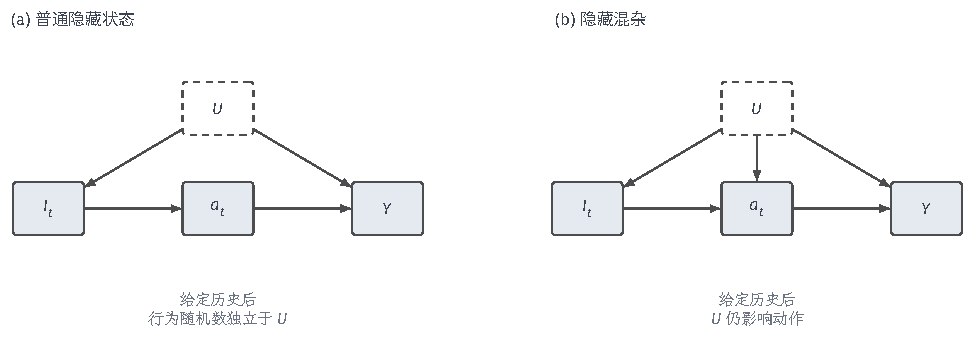
\includegraphics[width=163.714mm]{figures/10-reinforcement-learning/02-information-and-reward/tikz/rl-information-confounding.pdf}
  \caption{隐藏状态与隐藏混杂的区别。两图中的$U$均未记录，$I_t$为记录历史，$Y$为未来反馈。左图假设行为仅由$I_t$和独立随机数决定；右图多出$U\to a_t$，给定$I_t$仍不能阻断动作与后果之间的未记录共同原因。箭头表示因果假设。}
  \label{fig:rl-information-confounding}
\end{figure*}

有时可以用代理变量补充对隐藏量的间接观测，或增加传感器观测，但识别仍需明确的条件独立、可逆性或完备性等结构。字段变多不说明这些条件成立。部分POMDP离策略评价工作利用代理观测和矩阵秩条件处理隐藏机制，不能将这类结论改写为训练循环网络即可消除混杂\scite{rl4-tennenholtz2020-pomdp-ope}

% Outline: 4.6.3
\subsection{完全可识别时的历史表示与决策学习}
\label{sec:rl-information-full-identification}

先考虑不含上述隐藏混杂的一组条件：日志从回合开始完整保留$I_t$，行为以已知$\beta_t(a_t\mid I_t)$随机选择，给定历史后的随机数与潜在环境独立；目标也只使用记录历史，初始分布和环境共同，目标轨迹有行为支持。于是每个历史层内的动作按已知机制分配，物理状态隐藏不再给行为增加未知依据。我们可以据此计算目标与行为的可见回合记录比，获得点识别目标价值所需的校正。

隐藏状态本身并不阻止评价。仍用上面的$M_+$教学环境，若收集者不再按类型选动作，而是对每种类型都用独立公平随机数选$a_0$或$a_1$，两个动作组就都含有同样的总体类型混合。在总体上，$a_0$组奖励均值为$(1-1)/2=0$，$a_1$组为$(3+1)/2=2$，正好对应始终执行该动作的价值。状态类型仍不可见，改变的是动作组不再由类型挑选；正确随机化给出了将记录反馈用于目标行动的依据。

现在将第~\ref{sec:rl-information-estimators}~节的校正用于以可见历史为依据的策略。可见回合记录写成
\[
  \tau^o=(o_0,a_0,r_0,\ldots,o_H).
\]
给定历史和动作后的反馈分布记作$q(y_{t+1}\mid I_t,a_t)$。上述行为条件使目标与行为共享反馈因子。将轨迹密度按时间展开，再以目标密度除以行为密度，共同初始项和反馈项约去，得到
\begin{equation}
  \label{eq:rl-information-history-is}
  \frac{p_\pi(\tau^o)}{p_\beta(\tau^o)}
   =\frac{p(o_0)\prod_{t=0}^{H-1}
                  \pi_t(a_t\mid I_t)q(y_{t+1}\mid I_t,a_t)}
          {p(o_0)\prod_{t=0}^{H-1}
                  \beta_t(a_t\mid I_t)q(y_{t+1}\mid I_t,a_t)}
   =\prod_{t=0}^{H-1}\frac{\pi_t(a_t\mid I_t)}
                              {\beta_t(a_t\mid I_t)}.
\end{equation}
隐藏状态已在共同反馈因子中积分，因此最终只保留历史条件动作比。也可以先在完整隐藏轨迹上消去共同环境项，再求和隐藏状态；由于两策略的动作概率都只依赖可见历史，才能将它们提出该求和。

这一消去不能通过将$I_t$随意替换为$o_t$保留。行为若记住早期提示，只按当前画面拟合出的边缘频率就不是实际动作条件概率。专家若还看到例~\ref{ex:rl-information-confounding}~中的$U$，其动作项会随隐藏类型变化，无法从隐藏状态求和中提出，校正便失去依据。

识别条件成立后，可以直接按完整历史评价，或用有依据的充分表示降低计算成本。正确POMDP已知时用精确信念，预测结构可识别时可用PSR；潜在模型、循环或注意力记忆则需要检查允许动作上的预测或控制充分性。相应地，FQE可以在有限时域历史树上回归，行为约束作用于$\pi(a\mid I)$，提取动作时查询同一历史或经过论证的充分表示。直接保留历史减少了压缩假设，却可能使历史动作组合非常稀疏。

将完整历史换成$\bm z_t$，需要同时保留两种关系。一是目标策略和行为策略是否能从该表示确定实际动作概率，二是表示是否保留计算目标继续回报所需的历史差别。只证明网络能预测下一帧，不足以同时证明这两点；尤其不能把专家未记录的线索通过训练自动补进$\bm z_t$。识别是日志与生成条件提供的依据，表示是利用这些依据的计算选择。

这些计算仍有表示构造、行为概率估计、有限轨迹采样与优化误差，报告时应分开。训练用burn-in恢复记忆，部署却每$L$步清零，会变成不同策略；训练读到回合开始提示，部署只有窗口，也不是原来评价的对象。总体可识别排除了相同记录总体分布对应不同目标值的不唯一性，但在有限训练记录下，所选网络与优化程序仍未必给出准确估计。

早期提示任务可以将表示错误与不可识别分开。假设行为在每种提示下随机尝试两个出口，完整历史也被记录，则动作价值在总体上可识别。一个编码器保留$c$，另一个只重建走廊图像；延迟很长时，提示帧占平均重建损失的比例很小，两者重建误差可能相近。按原例不折扣成功奖励，前者仍可达到1，后者至多$1/2$。此时失败来自编码遗漏，不能解释为环境本来无法识别。

% Outline: 4.6.4
\subsection{部分可识别时的历史表示与决策学习}
\label{sec:rl-information-partial-identification}

若同一日志和结构仍容许多个价值，就需要保留定义~\ref{def:rl-information-identified-set}~中的一致模型集合$\mathcal M$，而不是选一个拟合模型当作唯一真相。对于固定$\pi$，比较$\mathcal M$内各模型的价值，取下确界和上确界，计算
$[\inf_MJ_M(\pi),\sup_MJ_M(\pi)]$，
作为识别集合的上下包络；也可改变允许的混杂强度，检查敏感性范围。包络只描述最小和最大边界，未必每个中间值都可实现。有限日志还须在外层加入总体分布未知的采样误差。

确定价值差的正负可能不必分别确定两个价值的数值。固定两个候选，在每个相同模型中先计算$\pi_1$价值减去$\pi_2$价值，再对$\mathcal M$取下确界。若这个最小边界仍为正，全部允许模型便给出同一排序；只看平均模型不够，因为另一个同样符合日志的模型仍可能反转次序。

\begin{example}[不知道共同偏移，仍知道谁更好]
  \label{ex:rl-information-partial-order}
  构造由$u\in[0,10]$参数化的一致模型，并令
  $J_u(\pi_1)=u+1$、$J_u(\pi_2)=u$。两个价值包络$[1,11]$与$[0,10]$大幅重叠，同一模型中的差却恒为1，因此$\pi_1$总较好。若将单独包络端点相减，$1-10=-9$对应为$\pi_1$取$u=0$、为$\pi_2$取$u=10$；这是松的包络差，不是任一共同模型的真实性能差。
\end{example}

\begin{theorem}[共同模型下的性能差确定排序]
  \label{thm:rl-information-partial-order}
  给定非空一致模型集合$\mathcal M$，在共同的任务、初始分布和时域口径下，假设两个固定候选策略在每个模型中的价值均为有限实数。若
  \[
    \inf_{M\in\mathcal M}
          [J_M(\pi_1)-J_M(\pi_2)]>0,
  \]
  则所有允许模型都给出$\pi_1$优于$\pi_2$的排序，两个单独价值区间即使重叠也不影响结论。
\end{theorem}

\begin{proof}
  将下确界记为$c>0$。定义保证任意同一个$M\in\mathcal M$均满足
  $J_M(\pi_1)-J_M(\pi_2)\geq c>0$，于是每个模型的排序相同。比较两策略时未切换模型，下确界也无须由某个模型取到，不等式仍成立。
\end{proof}

同一模型比较的要求与前面配对日志有相似的消差思路，但不确定性的来源不同。配对评价让两估计共用一条随机轨迹，可能消去采样波动；这里让两价值共用同一个尚未识别的环境，消去共同未知收益。增加独立日志可减小前者的波动，未必消除后者的模型歧义。两个单独区间因此不能不加判断地相减来替代共同模型差。

这里两候选共享未识别收益$u$，而“多得1”由额外结构假设给定，不能从拟合日志自行宣称。若允许策略只有$\pi_1,\pi_2$，为使选择在每个相容模型中都有依据，可以先各自对$u\in[0,10]$取最坏回报，再在两策略中最大化；最坏价值1和0会选中$\pi_1$。直接计算相对$\pi_2$的共同模型差下界则给出改进1。若另加不得偏离已覆盖历史的约束，且它排除了$\pi_1$的新历史，允许类只剩$\pi_2$，这项已由结构支持的改进也被放弃。保守限制可防止无依据推断，也可能因策略类过窄损失回报；系统的鲁棒优化见第~\ref{chap:rl-trustworthy}~章。

增加同类样本可以缩小采样误差，却不会自动排除总体上仍相容的模型。图~\ref{fig:rl-information-identification-width}~假设总体识别区间$[1,3]$，仅为示意将外层统计半径设为$2/\sqrt n$。样本增加时，外层范围缩到$[1,3]$而非单点。这是区分两种宽度的解析草图，不是算法经验曲线，也不是已经推导的置信保证。

\begin{figure}[htbp]
  \centering
  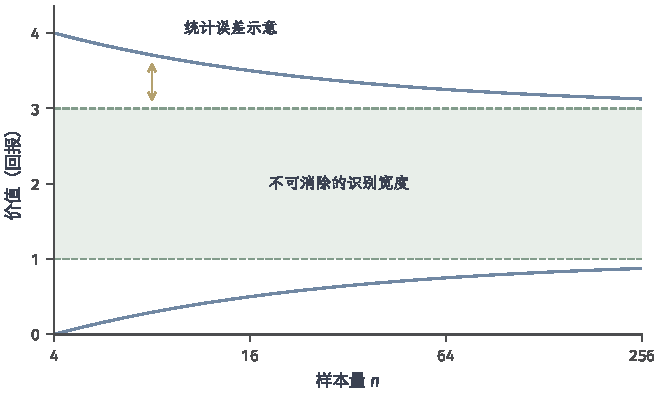
\includegraphics[width=112.000mm]{figures/10-reinforcement-learning/02-information-and-reward/matplotlib/rl-information-identification-width.pdf}
  \caption{教学识别区间$[1,3]$与示意外层范围$[1-2/\sqrt n,3+2/\sqrt n]$。实线范围随样本量缩小，虚线之间的非零宽度来自允许模型仍有差异；半径公式仅用于解释两种不确定性。}
  \label{fig:rl-information-identification-width}
\end{figure}

% Outline: 4.6.5
\subsection{不可识别时的学习边界与信息补充}
\label{sec:rl-information-unidentifiable}

若一致模型仍支持相反排序，当前目标决策就没有被识别。例~\ref{ex:rl-information-confounding}~的日志在两个模型下似然完全相同，最优动作却分别为$a_0$、$a_1$；缺口是专家选择所依据的未记录类型及其他动作的反事实后果。更细的当前观测编码不会补出未记录的类型及各类型下未尝试动作的后果，复杂模型收敛到任一解释也不能证明排序正确。

可以通过收缩目标或补充依据继续推进。缩小$\Pi$只比较日志支持的策略，或将全局最优改为基线附近的有限决策，改变的是要回答的问题。增加已知动力学、行为随机化或代理观测等可核验假设，改变的是允许模型集合。新假设须有外部依据才能排除相容解释，方便拟合的设定不能冒充原日志中的事实。

\begin{table*}[htbp]
  \centering
  \small
  \begin{tabularx}{\linewidth}{p{26mm}XX}
    \toprule
    缺失的记录或模型约束 & 可补采字段或补加假设 & 仍须核验的条件 \\
    \midrule
    较早提示未记录 & 从真实回合开始的长历史或足够记忆摘要 & 提示是否确实保留；部署可用性与回合边界一致 \\
    行为机制不明 & 当时动作概率、策略版本及相关上下文 & 动作概率所依据的历史字段完整且正确；潜在类型上的支持仍可能缺失 \\
    当前状态混叠 & 新传感器、主动辨识动作或代理变量 & 新观测能否区分与控制有关的状态；代理识别条件 \\
    目标行为无覆盖 & 受控随机交互、指定区域的实验 & 查询确实覆盖目标历史动作；代价和安全权限允许 \\
    初始或任务条件不明 & 初始状态、目标及采样分层元数据 & 评价分布与部署分布一致，或有正确校正 \\
    \bottomrule
  \end{tabularx}
  \caption{补采字段与补充假设要对应具体缺口。记录隐藏类型可以消除部分混杂，却未必补齐每种类型下未尝试的动作；新增字段与新增行为各有不同作用。}
  \label{tab:rl-information-information-repair}
\end{table*}

表~\ref{tab:rl-information-information-repair}~逐项对应了可补采的日志字段或补加的结构假设。单独补记概率未必够：例~\ref{ex:rl-information-confounding}~中专家在每种类型上都确定性行动，即使记录$U$，该类型的另一动作仍无支持。识别固定策略价值，还需在允许类型内受控随机行动，或有依据的跨类型、跨动作结构。更长的同类日志不能替代这些行为概率字段或模型结构假设。

若允许有限交互，可以分别安排状态辨识与策略验证预算。辨识选择能区分相容模型的传感或动作，并在需要时更新表示；验证则固定新策略、其可读取的历史及记忆初始化协议，取得独立的策略回报证据。自适应辨识取得的记录不能未经处理便当作独立最终测试。权限不足，或新反馈仍在相容环境中同分布时，无法判断的结论应保留。网络容量可帮助降低表示或拟合误差，却不能仅凭同分布的可见记录辨清本来不可区分的环境。

% Outline: 4.7
\section{本章小结}
\label{sec:rl-information-summary}

章首的小车问题现在可以分别回答。速度不可见时，需要由历史保留线索，或用信念与记忆形成决策依据；缺少左转经验时，需要检查收集机制与覆盖，判断左转后果能否从日志确定。Tiger说明模型已知仍可能值得付费辨认当前状态，未覆盖动作反例则说明状态完全可见也仍可能无法识别价值。仅增加记忆不能补齐动作后果，仅补充同类行为也不能找回未记录的线索。

排除了同样日志对应不同答案的歧义以后，还需要用有限记录计算价值；这一步会有样本波动、行为概率误差和模型误差。再用估计值改策略时，策略可能主动寻找高估动作，因此还要检查估计是否覆盖新的选择。行为约束限制策略偏离日志记录中的行为，悲观目标扣除未证实的收益，二者都需要自己的误差依据。最后评价的对象是实际提取出的执行策略，不能用价值网络的训练损失或模型内回报替代它。答案能够确定、数值能够估计、目标能够优化和策略能够验证，分别跨过了不同的障碍。

两类限制叠加时，执行历史、日志字段和收集者选动作的依据要共同核对。在完整历史、共同环境与初始条件、正确随机化机制和目标支持下，隐藏状态可从共同反馈项中积分，概率比只含历史条件动作概率。存在未记录行为依据时，相同日志却可能对应相反排序。部分识别仍可能通过共同模型差作出有限决策，排序不可识别时则需收缩结论或补采能区分候选模型的反馈或补加有依据的结构约束。随策略结论报告执行策略可读历史、日志机制、覆盖范围、表示假设、查询预算及误差依据，才能确定它适用于哪里。

\chapter{奖励受限下的强化学习}
\label{chap:rl-reward}

一台配送机器人已经学会移动和避障，但这只解决了“能做什么动作”；我们还必须告诉它“什么样才算一次好的配送”。前几章默认环境每步都会返回一个可信的数值奖励，本章要处理的正是这个奖励本身出问题的情形。请人示范路线可以提供可用动作，但示范者选择电梯，可能为了更快，也可能为了省电或保持包裹水平——单凭动作记录，背后的计分标准未必已经确定，还需要进一步判断这些记录究竟支持哪一种目标解释。

即使已经明确约定“正确签收且包裹完好”、也能拿到可靠的总分，学习仍有困难：终局失败只告诉我们这次配送坏了，却没有直接标出是核对、装载还是搬运哪一步出的错，需要想办法把最终结果联系回早期决策。反过来，如果贪图反馈及时，改成每移动一米就给分，反馈倒是又快又密，机器人却可能靠不停地绕路刷高分、根本不去交付——这是数值标准本身定错了，靠增加反馈或加快传播都无法补救。因此，反馈“表达了什么”“能否说明每一步的局部贡献”“是否真的符合我们想要的行为”，是三个必须分别解决的问题。

第~\ref{chap:rl-learning}章虽然不知道期望奖励是多少，但仍假定每次交互后都能读到一个奖励样本；第~\ref{chap:rl-information}章则检查能看到哪些观测、历史记录是否完整，以及日志的状态动作覆盖是否足以支持决策。本章保留前两章的全部学习工具，只改变喂给它们的反馈。我们要分别判断三件事：当根本没有可信的标量奖励时，示范、偏好、检查等其他记录能约束哪些行为目标；当只有一条轨迹的总分时，怎样用它更新中途的局部决策；当训练分数确实提高时，实际行为是否真的满足了最初的要求。图~\ref{fig:rl-reward-map}说明这三个问题如何共同支撑反馈学习。它们是可以叠加的限制，而不是必须排队依次排除的三种故障。

\begin{figure*}[htbp]
  \centering
  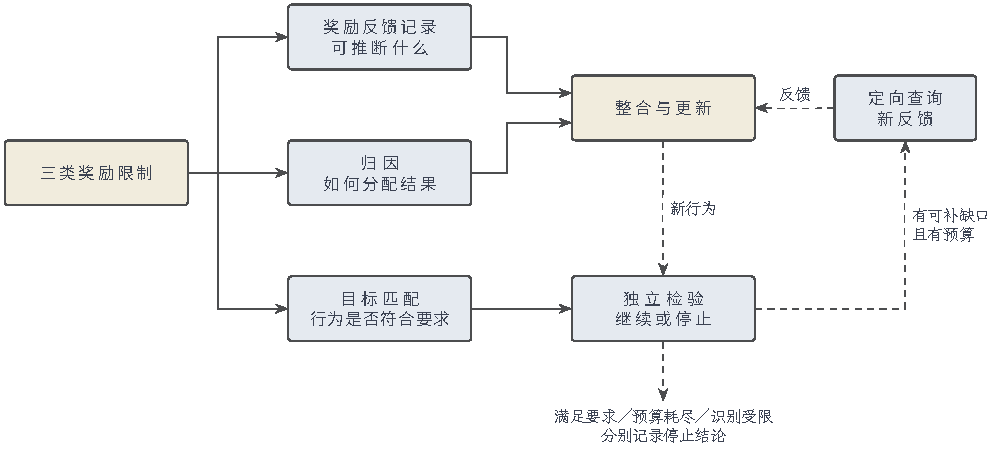
\includegraphics[width=169.000mm]{figures/10-reinforcement-learning/02-information-and-reward/tikz/rl-reward-map.pdf}
  \caption{三类奖励限制与反馈学习的关系。实线表示观测、归因和目标匹配分别为反馈整合、策略更新及行为检验提供依据，不规定三者的解决顺序；虚线表示取得新行为和新反馈后进入下一轮。停止可能因为证据已满足要求，也可能因为预算耗尽或区分候选奖励所需的反馈无法取得，三者支持的结论不同。}
  \label{fig:rl-reward-map}
\end{figure*}

本章仍用$r_t$表示执行$a_t$后的奖励，用$J(\pi)$表示未归一化的期望折扣回报。为观察反馈落在哪个环节，我们另设一个四步配送任务：机器人依次核对包裹、装载、搬运和交付，状态包含包裹身份、位置及完好情况。这个案例不沿用前文随机网格的精确动力学；除特别说明外，反馈在交付后才给出。本章用于计算的人工数字都是教学假设。

% Outline: 5.1
\section{奖励信号的三类限制}
\label{sec:rl-reward-limits}

% Outline: 5.1.1
\subsection{奖励观测受限}
\label{sec:rl-reward-observation}

机器人不知道一条路线的平均耗电量时，仍可在每次执行后读电表、再用样本均值估计期望耗电。若固定路线、负载及其他运行条件，独立重复执行，且耗电量的期望有限，就可以用可信的电表读数估计同一条件下的期望耗电；有限次执行仍有抽样误差。这仍是第~\ref{chap:rl-learning}章讨论过的未知奖励期望估计。但若目标改为“把包裹妥善交给收件人”，而日志里只记录了移动距离，问题的性质就变了：距离既没说明交给了谁，也没说明包裹有没有破损。此时缺少的是能够表达目标的观测，而不是均值估得不够精确——收集再多的距离记录，也判断不了交付质量。

同一次配送其实可以留下多种不同记录：专家当时怎样装载（示范了一个动作）、收件人给这次配送打几分（一个评分）、两条路线哪条更合意（一次比较）、包裹编号是否通过核对（一次检查）。它们绝不是四种等价的“正确标签”：动作记录描述已经发生的行为，评分给出某个尺度上的数值，比较只给相对先后，检查则只判断某个指定条件成不成立。因此必须先说清每条记录评价的对象，才能决定它应该进入动作拟合、奖励学习还是条件验证。

\begin{definition}[替代反馈的形式与粒度]
  \label{def:rl-reward-feedback}
  \term{示范}（demonstration）记录决策者实际采取的行为，可以是某状态上的动作，也可以是整条轨迹。\term{评分}（rating）按照约定尺度给被评价对象一个数值。\term{偏好}（preference）记录在相同比较条件下，评价者如何排列两个或多个对象。\term{验证反馈}（verification feedback）判断对象是否满足指定条件，并可附带检查证据。反馈的\term{粒度}（granularity）是这次判断实际评价的单位，可以是动作、步骤、轨迹片段或完整轨迹。记录到达的时间不必等于被评价动作发生的时间。
\end{definition}

粒度和到达时间是两回事，不能混为一谈。签收之后才补记一条“装载时身份错误”，它评价的仍是装载那一步，只是这条记录到达得晚；而“这次配送 0 分”评价的是整条轨迹，并不等于给每一步都打上了 0 分的标签。把一个轨迹总分送进各步的策略更新，本质上是在用总结果去估计各动作的影响（这是下一节奖励归因要处理的事），并没有自动把评价对象细化到每一步。

这四种记录描述的行为和评价内容各不相同。示范只告诉我们“当时做了什么”，对没有选择的动作毫无评价；带等距尺度的标量评分还能表达评价之间的差距，但若分数只是有序等级（比如一星到五星只表示好坏次序），数字之差就不再自动对应评价之差——把等级用于期望回报前，必须显式规定等级到训练效用的编码方式。偏好可以只给顺序而不给绝对分数；验证器的“通过”标记则只支持被检查的那一个条件。表~\ref{tab:rl-reward-forms}还单列了查询权限：读取已有的示范记录，与获准继续向专家追问，是两种不同的访问能力，前者不能代替后者。

\begin{example}[等级排序没有确定期望效用]
  \label{ex:rl-reward-ordinal-score}
  策略甲各以$1/2$概率得到1星和5星，策略乙总得4星。直接按星数计分时，甲的期望分为3，乙为4。若星级只表达次序，将1、4、5星分别编码为0、1、100仍保留这些等级的排序，此时甲的期望为50，乙为1，比较结果反转。因此，等级次序本身没有确定怎样比较这两种随机结果；按平均星数优化，可以作为任务方明确选择的训练目标约定。
\end{example}

\begin{table*}[htbp]
  \centering\small
  \begin{tabularx}{\linewidth}{@{}>{\raggedright\arraybackslash}p{17mm}*{5}{>{\raggedright\arraybackslash}X}@{}}
    \toprule
    形式 & 反馈对象 & 粒度 & 噪声来源 & 查询权限 & 可推断对象 \\
    \midrule
    示范 & 已执行动作与上下文 & 动作、轨迹 & 次优专家、漏记任务指令或专家当时可见的状态 & 固定日志或另行授权的专家查询 & 行为条件分布；附加理性假设下的奖励约束 \\
    评分 & 单个被评价行为 & 步骤、片段、轨迹 & 尺度漂移、反应延迟 & 可只提供历史评分 & 该尺度下的评价函数 \\
    偏好 & 同条件候选行为 & 一对片段或轨迹 & 次序效应、偏好异质性 & 固定比较或主动选对 & 比较概率、相对效用 \\
    验证 & 产物或状态关系 & 步骤、结果 & 规则遗漏、执行误差、误判 & 可离线复查或在线调用 & 指定条件的通过情况 \\
    \bottomrule
  \end{tabularx}
  \caption{四种反馈形式及其记录对象。形式说明记录表达什么，查询权限说明还能补充什么。人类、AI、规则和执行器描述反馈来源，同一来源可以产生多种形式。}
  \label{tab:rl-reward-forms}
\end{table*}

例如，人和模型都可以提供示范、评分或成对偏好。身份核对规则可以返回通过标记，实际执行开箱操作的检查器也可以返回破损结果。这里“人类反馈”回答谁在判断，“偏好反馈”回答判断怎样记录，两者可以同时描述同一条记录，不是互斥类别。

% Outline: 5.1.2
\subsection{奖励归因受限}
\label{sec:rl-reward-credit-limit}

假设日志已经准确记下“包裹完好、交付成功”，我们仍然不知道这份成功里哪些先前决策值得强化：核对身份、平稳搬运、甚至选了一条容易的路线，都可能与成功同时出现。\term{奖励归因}（reward credit assignment）要做的，就是把长期结果联系回此前的具体决策，为每一步的局部更新提供“贡献”判断。第~\ref{chap:rl-learning}章已经用回报、TD 误差和优势估计来传播结果；本节则要进一步检查这些工具实际读到了哪些结果评分和过程标签，以及还有哪些贡献始终没有被观测到。

四步配送如果只在最后才得到成功分，那么前三步即时奖励为 0，但这个 0 既不表示它们没有贡献，也不表示检查器判定它们出错——它只说明当前的计分规则还没有给出对早期步骤的局部评价。要更新早期动作有两条不同的路子：一是把终局结果沿动作概率的梯度回传（传播已有结果），二是补充新的过程检查（取得新的评价证据）。

\begin{table*}[htbp]
  \centering\small
  \begin{tabularx}{\linewidth}{@{}>{\raggedright\arraybackslash}p{27mm}*{3}{>{\raggedright\arraybackslash}X}@{}}
    \toprule
    现象 & 缺口 & 主要影响 & 不能直接推出什么 \\
    \midrule
    非零奖励很少 & 多数尝试没有区分信号 & 难以探索到成功轨迹 & 一旦成功就能正确归因 \\
    反馈延迟长 & 行动与反馈相隔许多步 & 贡献需跨步传播；随机轨迹下估计可能更难 & 回报方差必然增大或反馈语义错误 \\
    只有轨迹总分 & 局部贡献未被观测 & 无关动作也可能分享相同结果 & 每一步都有独立监督 \\
    反馈噪声大 & 相同行为的判断不稳定 & 估计方差和误排序增加 & 噪声一定来自时间延迟 \\
    \bottomrule
  \end{tabularx}
  \caption{影响奖励归因的四种反馈性质。非零奖励少、反馈来得晚、只评价整条轨迹及判断有噪声，可以在同一任务中同时出现，但各自造成的缺口不同。}
  \label{tab:rl-reward-credit-limits}
\end{table*}

反馈到达得晚，不等于回报方差必然增大。确定性终局得分无论晚到多少步，方差仍为零。若固定策略和随机得分$X$的分布，只把奖励发生时刻从0移到$h$，在固定$\gamma<1$下，折扣回报的方差为$\gamma^{2h}\operatorname{Var}(X)$，反而不大于原方差。较长交互中，随机状态、动作及评分噪声可能使局部贡献更难估计；判断方差怎样变化时，必须固定所比较的估计量及其他条件。若只是记录晚到、奖励所属时刻不变，离线计算的回报也不会因此改变。

按照表~\ref{tab:rl-reward-credit-limits}，我们可以先区分尚未找到成功行为与已经找到成功行为却不清楚贡献这两种情况。机器人始终找不到收件人时，增加探索或提供成功示范可能补上行为线索。若日志中已有许多成功配送，但身份核对总与无关的扫码动画一起出现，就需要辨认哪一个动作影响结果。重复收集相同组合未必能区分二者；给每次动画播放加分虽然增加了反馈频率，也没有提供能区分各动作贡献的评价依据。

% Outline: 5.1.3
\subsection{奖励与行为目标不匹配}
\label{sec:rl-reward-mismatch-limit}

若计分规则是“每移动一米得一分”，机器人就能靠不断绕圈把回报刷得很高，却始终不完成配送。这里要特别注意：优化器并没有失灵，它正忠实地最大化给定分数；出问题的是数值标准本身没有表达交付要求。要诊断这种偏差，必须把两件事分开——我们真正希望发生的行为，与训练实际在优化的数值。

\begin{definition}[奖励、回报、效用与行为要求]
  \label{def:rl-reward-objective}
  单步奖励$r_t$是交互协议返回的标量，累计回报$G_0=\sum_t\gamma^t r_t$按约定的时间权重汇总这些标量。\term{效用}（utility）表示决策者如何评价结果或结果分布，可记为$u(\tau)$或策略评价泛函$\mathcal U(\pi)$，不预设它等于$J(\pi)$。\term{行为要求}（behavioral requirement）规定希望发生什么以及在什么条件下发生，例如交给正确收件人、保持包裹完好并满足能耗要求。\term{代理奖励}（proxy reward）是训练所用的数值编码；它是否表达了这些要求，须用独立证据检验。
\end{definition}

据此再看三种限制：里程计分即使即时且准确，也可能遗漏任务目标；“正确收件人且完好”的终局标记可以表达明确的成功条件，但早期动作要经过多步才得到反馈。有效路线示范能够帮助行动，却未必确定各项奖励权重。同一任务还可以同时具备三种限制，例如示范不记录破损、评分延迟到终局，训练又额外奖励里程。

选择学习办法要先定位缺口。缺少可靠信号时需要补充能表达目标要求的示范、评分、偏好或验证结果，缺少局部贡献时需要检查结果怎样进入更新，标准遗漏要求时则需要修订目标。训练损失下降只能说明模型更符合所选训练准则，不能同时证明反馈覆盖充分、归因正确和编码完整。交付身份、完好情况及能耗的独立检查应在优化前约定；若事后随行为改变标准，就失去了判定偏差的共同依据。这一判断以配送要求、可接受行动及评价条件已经约定为前提：代理分数只是要求的数值表达，目标是否达成仍需对相应行为和结果取证。目标、训练信号与行为边界的区分可参考\BookChapterRef{chap:trust-alignment}{卷3《基础、理论与可信性》中讨论目标对齐与行为约束的章节}。

% Outline: 5.2
\section{奖励观测受限下的强化学习}
\label{sec:rl-reward-alternative}

假设配送日志拿不到可靠的逐步奖励，但保留了专家路线、两条路线的比较或签收检查结果。这时可以走三条不依赖唯一奖励的路子：直接用动作示范拟合策略、用偏好约束效用的相对大小、或用验证结果构造策略更新信号，而不必先反推出一个唯一的数值奖励。每种反馈究竟能约束什么，完全取决于记录实际表达的内容以及它在什么假设下产生。

% Outline: 5.2.1
\subsection{替代反馈与可推断对象}
\label{sec:rl-reward-inference}

在同一个配送任务中，示范可以记录专家选择电梯，偏好可以记录收件人更喜欢平稳但较慢的配送，身份验证则只检查是否交给正确的人。选择电梯没有单独说明“慢一些更好”，身份通过也没有证明包裹无破损。若把这些记录统一改成“正例”，我们就无法再分清它们支持哪种结论、排除了哪种目标解释。

当状态在示范与部署时都可读取、且两者使用相同状态字段时，策略$\pi(a\mid s)$给出某状态上的动作分布，占用度量$d^\pi(s,a)$汇总长期访问状态和动作的概率；价值$V^\pi,Q^\pi$预测给定奖励和策略下的后续回报。奖励$R(s,a)$规定单步期望计分，效用表达评价者怎样看待结果。状态不可见时，执行策略只能以部署可得历史$I_t$为依据，不能把训练日志中的特权状态直接作为部署时可读取的决策依据。这些对象相互联系，但一条记录对其中一个对象施加约束，并不自动唯一确定其他对象。表~\ref{tab:rl-reward-inference}列出各类记录可以支持的学习对象。

\begin{table*}[htbp]
  \centering\small
  \begin{tabularx}{\linewidth}{@{}>{\raggedright\arraybackslash}p{22mm}*{4}{>{\raggedright\arraybackslash}X}@{}}
    \toprule
    反馈 & 候选推断对象 & 额外假设 & 训练交互 & 拟合所得对象 \\
    \midrule
    状态动作示范 & 策略 & 记录的状态或可得历史足以确定专家的条件动作分布，覆盖可用 & 行为克隆不需要 & 动作分布 \\
    专家与策略轨迹 & 占用、软价值 & 共同环境，轨迹采样口径一致 & 占用匹配通常需要 & 策略或价值函数 \\
    专家轨迹 & 奖励、特征期望 & 专家理性、奖励函数类、动态模型 & 需规划或采样权限 & 奖励候选及策略 \\
    标量评分 & 评价函数 & 尺度、对象与时间归属明确 & 拟合本身不需要 & 评分预测器 \\
    成对偏好 & 效用差、策略 & 比较模型与共同条件 & 拟合可离线；在线RL另需新采样 & 奖励模型或偏好策略 \\
    过程、结果验证 & 条件通过概率 & 规则有效、检查前提满足 & 在线更新需可调用验证 & 验证信号与策略 \\
    \bottomrule
  \end{tabularx}
  \caption{不同记录可支持的推断、假设及所得模型或策略。同一反馈可以用于多个学习对象，同一对象也可以结合多种反馈。“不需要交互”只说明拟合阶段的访问要求，不表示固定示范记录已覆盖新策略将访问的状态和动作。}
  \label{tab:rl-reward-inference}
\end{table*}

一个单步例子即可看出不唯一性。任务只有左、右两个动作，专家总选左；奖励$(R(\text{左}),R(\text{右}))=(1,0)$和$(10,9)$都能使左最优。若记录只保留甲、乙、丙的确定排序，效用$(3,2,1)$和$(100,2,0)$也都给出甲优于乙、乙优于丙，但它们的效用差不同，未必在同一个随机偏好模型中产生相同比较概率。排序只给出先后次序，完整比较概率还给出选择频率；即使概率已知，共同加法常数等歧义通常仍然存在。

新增查询能否解除歧义，取决于它提出了什么新问题。若允许主动查询，我们可以比较此前未比较的路线，或询问专家在当前策略偏离后怎样恢复。按同一采集或评价协议取得新的独立记录，并满足相应矩条件时，可以提高已涉及行为的估计精度；仅重复使用已有记录不会增加这类统计证据，也不会补出从未涉及的要求。能识别的是动作、排序还是奖励，仍须按记录内容及生成假设分别判断。

% Outline: 5.2.2
\subsection{从示范直接学习策略}
\label{sec:rl-reward-bc-dagger}

专家既然已经给出了可用动作，最直接的想法就是让自己的策略在相似状态、或在部署时能读到的相同历史下复现这些动作。前一章把“拟合日志里实际采取的动作”称为\term{行为克隆}（behavioral cloning, BC）；在这里，它把示范记录中的状态（或可得历史）当作条件变量，把专家动作当作监督标签，本质上是一个监督学习问题。要衡量一个离散动作策略复现示范的程度，可以惩罚它给专家动作分配的概率太小。设任务有$t=0,\ldots,H-1$共$H$步，专家在各时刻访问状态的分布为$\nu_t^{\mathrm E}$；对这些状态以及专家在其中选择的动作取期望，再对时间平均，得到总体负对数似然
\begin{equation}
  L_{\mathrm{BC}}(\bm{\theta})
  =-\frac1H\sum_{t=0}^{H-1}
  \mathbb E_{\substack{s\sim\nu_t^{\mathrm E}\\
              a\sim\pi_{\mathrm E}(\cdot\mid s)}}
       \log\pi_{\bm{\theta}}(a\mid s).
  \label{eq:rl-reward-bc}
\end{equation}
最小化该损失，就是在专家访问分布上最大化示范动作的平均对数概率，并不要求每条记录的概率都同时增加。训练时用专家示范训练样本$D_{\mathrm E}$的平均负对数似然估计这个期望，其中$D_{\mathrm E}$是按声明采集机制取得的有限示范记录组；候选策略类给出允许的条件动作分布，学习规则还要规定目标构造、初始化、更新、停止与策略读出。训练拟合与独立评价使用不同职责的样本，不能仅凭训练动作似然较高断言部署回报改善。一次参数更新可写为
$\bm{\theta}^{(k+1)}=\bm{\theta}^{(k)}
-\eta\nabla_{\bm{\theta}}\widehat L_{\mathrm{BC}}$，
完成一次参数拟合，其中$\eta$为步长。这些示范记录由专家产生，不是当前策略执行得到的；每次遍历都要为记录计算策略概率和梯度，但不需要奖励标签或重新运行环境。

连续动作还可以用平方误差$\mathbb E\lVert f_{\bm\theta}(s)-a\rVert_2^2$拟合动作数值；在无限容量下，最小化这个误差得到的是条件均值。但均值动作未必能用。设想专家绕障时等概率选择$-1$和$1$（左绕或右绕），两者都是有效路线，可它们的均值$0$却可能让机器人直冲障碍。要保留示范中的多种可行动作模式，就得显式表示一个多模态的动作分布，而不能只输出平均动作。均值出错还可能有另一个原因：日志漏记了任务指令，导致相同观测其实对应不同的专家动作；这种情况下单纯加大网络也无法恢复未记录的指令。

即使动作在专家示范覆盖的状态上拟合得很准，也不能保证策略实际运行时同样准。这里存在一个被称为“复合误差”的现象：专家几乎不会走进错误走廊，因此示范里没有那些状态；而克隆策略只要偶发走错一步，就会落入示范从未覆盖的状态，此后只能在陌生状态上继续决策、往往又走错，错误于是一层层累积。为看清早期错误为何代价更大，下面在共同环境中比较专家与学习策略，用“第一次与专家分歧”的概率给出一个保守上界。

先看$H=4$的尺度。若在第一步选错走廊，后面四步都可能付额外成本；若直到最后一步才与专家不同，只剩一步可能受影响。将每个可能分歧位置的最坏后果分别累计，出现$4+3+2+1=10$这个系数。若每个专家状态分布上的分歧概率至多$0.05$，相应保守成本差界为$0.5$。这不是每次错误都实际损失余下全部成本，而是用单步成本上限控制最不利情况；下面正式说明概率条件。

\begin{theorem}[行为克隆的首次分歧界]
  \label{thm:rl-reward-bc}
  给定正整数$H$和$\varepsilon\geq0$。考虑共同非空有限状态集、各状态非空有限合法动作集、共同初始分布与共同转移核的$H$步任务，每步成本$c_t(s,a)\in[0,1]$，总成本记为
  $C_H(\pi)=\mathbb E_\pi\sum_{t=0}^{H-1}c_t(s_t,a_t)$。
  专家动作映射为$g_{\mathrm E}$，其诱导策略为$\pi_{\mathrm E}(\cdot\mid s)=\delta_{g_{\mathrm E}(s)}$；记该策略在时刻$t$的状态分布为$\nu_t^{\mathrm E}$。若合法Markov学习策略$\pi$在每个专家状态分布上均满足
  \[
    \mathbb E_{s\sim\nu_t^{\mathrm E}}
    \bigl[1-\pi(g_{\mathrm E}(s)\mid s)\bigr]\leq\varepsilon,
  \]
  则
  \[
    C_H(\pi)-C_H(\pi_{\mathrm E})
    \leq \frac{H(H+1)}2\varepsilon.
  \]
  非平稳专家可把时间加入状态，结论不变。
\end{theorem}

\begin{proof}
  将两条轨迹放在同一概率空间中，使它们从相同状态出发，并在尚未出现动作分歧时共用环境转移的随机性。另在完整专家轨迹的每个$s_t^{\mathrm E}$上，抽取服从$\pi(\cdot\mid s_t^{\mathrm E})$的候选动作。令$B_t$表示该候选动作不同于专家动作；定理假设给出$\mathbb P(B_t)\leq\varepsilon$。

  首次分歧以前，两条轨迹的状态、动作和成本相同，所以截至$t$已发生分歧，只可能是在某个$j\leq t$出现了$B_j$。这个事件包含于$\bigcup_{j=0}^{t}B_j$，由并集界，其概率不超过$(t+1)\varepsilon$。分歧后两条轨迹可以任意发展，但单步成本均在$[0,1]$内，额外成本至多为1；未分歧时额外成本为0。对这一指示变量上界取期望，再按时间求和，
  \[
    C_H(\pi)-C_H(\pi_{\mathrm E})
    \leq\sum_{t=0}^{H-1}(t+1)\varepsilon
    =\frac{H(H+1)}2\varepsilon.
  \]
  并集界使用的是完整专家轨迹上的事件概率，并未假定“此前尚未分歧”条件下的错误率也等于$\varepsilon$，因此没有额外引入条件分布假设。
\end{proof}

由于每步成本至多为1，总成本差本身还不超过$H$，可以将界的右端取为$H$与上述二次项中的较小值。二次项来自一次早期分歧可能影响余下多步的估计，不是所有任务都会二次恶化的断言；若机器人能迅速恢复，实际额外成本可以小得多。

复合误差的根源是专家轨迹与学习策略执行轨迹所访问的环境状态分布不一致。一个自然的补救办法，是让专家专门对学习策略实际误入的状态补动作标签。\term{数据集聚合}（Dataset Aggregation, DAgger）反复执行当前策略、就它访问到的状态向专家查询，再把新标签对应的状态动作记录追加到训练样本中重新拟合。它改变的是交互训练记录的状态覆盖范围，使偏离后的状态也进入下一轮训练，而不是只在专家原有轨迹附近打转。图~\ref{fig:rl-reward-dagger}分别画出执行、查询和聚合三步；Ross 等给出了这一归约及其在线学习分析\scite{ross2011}。

\begin{algorithm}[一轮DAgger更新]
  \label{alg:rl-reward-dagger}
  \begin{algorithmic}[1]
    \Require 已聚合训练记录$D^{(k)}$，策略$\pi^{(k)}$，专家查询接口，轨迹预算$m$
    \Ensure 新增训练记录$D^{(k+1)}$与候选策略$\pi^{(k+1)}$
    \State 在获准环境中执行$m$条$\pi^{(k)}$轨迹，记录实际访问的状态
    \State 对这些状态查询$a_{\mathrm E}=g_{\mathrm E}(s)$，保留失败及偏离后的状态
    \State 将新标注记录$(s,a_{\mathrm E})$追加到$D^{(k)}$，保留重复记录，得到$D^{(k+1)}$
    \State 在聚合训练记录上最小化模仿损失，得到$\pi^{(k+1)}$
    \State 在独立轨迹上评价任务表现，并记录查询数与执行风险
  \end{algorithmic}
\end{algorithm}

\begin{figure}[htbp]
  \centering
  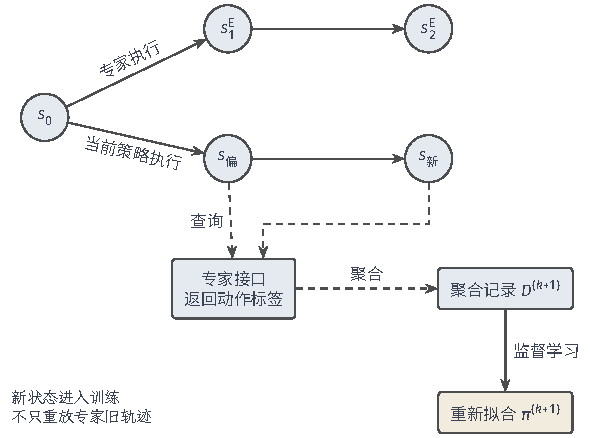
\includegraphics[width=99.977mm]{figures/10-reinforcement-learning/02-information-and-reward/tikz/rl-reward-dagger.pdf}
  \caption{DAgger补充当前策略偏离后的状态。两条轨迹从同一起点出发，分歧后对当前策略访问的新状态查询专家；新标签随追加后的状态动作训练记录进入下一轮。查询只取得动作标签，不表示专家已在环境中执行该动作。}
  \label{fig:rl-reward-dagger}
\end{figure}

例如，当前策略误入$s_{\text{偏}}$，专家标注“返回”。在二动作策略中，用logit $z$表示返回的对数几率，返回概率为$\sigma(z)$，其中$\sigma(z)=(1+\exp(-z))^{-1}$将实数转换为概率。若当前$z=0$，该标签的负对数似然梯度是$\sigma(0)-1=-1/2$；以$0.2$为步长下降，得到$z=0.1$，返回概率由$0.5$升至约$0.525$。这次更新利用了原专家示范未覆盖的错误状态。取得这些标签也有成本：每轮执行$m$条$H$步轨迹需要$mH$个环境步、至多$mH$次查询，并要重新拟合不断追加的训练记录组。

能否持续改善自身访问分布上的模仿损失，可以用在线学习的遗憾来描述：每轮损失在该轮策略访问分布上计算，比较基准则是预先指定策略类$\Pi$中，同一策略在全部轮次上的平均损失。若这些总体损失可直接获得，平均遗憾小意味着迭代策略的平均损失接近类内最小值，因而至少有一轮不超过该平均上界。

\begin{theorem}[理想化DAgger的无遗憾归约]
  \label{thm:rl-reward-dagger}
  固定正整数$H,K$、共同环境中的非空候选策略类$\Pi$，以及非负可测的模仿损失$\ell:\Pi\times S\to[0,\infty)$；假设下面各项期望均为有限实数，并给定有限常数$\varepsilon_{\mathrm{reg}}$。令$\nu_t^{\pi^{(k)}}$为第$k$轮策略在时刻$t$的状态分布，
  $\bar\nu^{(k)}=H^{-1}\sum_{t=0}^{H-1}\nu_t^{\pi^{(k)}}$，并定义
  $\ell_k(\pi)=\mathbb E_{s\sim\bar\nu^{(k)}}\ell(\pi;s)$。若$K$轮在线拟合满足
  \[
    \frac1K\sum_{k=1}^K\ell_k(\pi^{(k)})
    -\inf_{\pi\in\Pi}\frac1K\sum_{k=1}^K\ell_k(\pi)
    \leq\varepsilon_{\mathrm{reg}},
  \]
  则至少一轮$k$满足
  \[
    \ell_k(\pi^{(k)})
    \leq\inf_{\pi\in\Pi}\frac1K\sum_{j=1}^K\ell_j(\pi)
        +\varepsilon_{\mathrm{reg}}.
  \]
\end{theorem}

将遗憾不等式中的比较项移到右侧，就得到各轮自身分布损失的平均上界。再在实际生成的$K$个策略中取损失最小的一轮，利用
\[
  \min_k\ell_k(\pi^{(k)})
  \leq\frac1K\sum_k\ell_k(\pi^{(k)}).
\]
即可得到定理的结论。比较策略在所有轮次的分布上评价，分布本身不必相同。这个结果首先约束模仿损失；使用有限样本还要加入估计误差，混合执行专家时还要控制混合分布与自身分布的差异。若进一步推成任务成本界，需要模仿损失能控制动作错误，并且一次错误后专家恢复的额外成本有统一上界。平均遗憾条件本身不足以保证任意实现都具有线性时域成本界。实现时可以保存各轮候选，并按预先分配的预算，用独立验证回合比较它们；若选择依据是各候选自身访问分布上的模仿损失，还需为这些状态取得专家动作标签。验证误差须对参与选择的候选共同受控，选定后再用未参与选择的测试回合报告表现。若按任务回报选择，应另报告该指标的评价依据，不能把模仿损失的存在性结论直接当作任务回报保证。

动作模仿得像，不等于动作的后果代价相同。机器人“走错一条可以立刻返回的支路”和“把包裹交给错误的收件人”，在动作标签上都可能被记为与专家不符，但前者只多走几步、可以轻易挽回，后者却可能无法撤回。要在这两种错误之间合理地分配更新，光知道专家的正确动作还不够，还必须知道候选动作之后的长期代价。仅有动作标签时，DAgger 无法区分两种错误动作的后续代价；于是需要代价敏感的模仿或后续价值查询。\term{基于搜索的结构化预测}（search-based structured prediction, SEARN）将序贯预测转为代价敏感学习，通常通过后续执行估计各动作的代价；其中SEARN是方法专名，不是该英文名称逐词首字母的缩写。\term{聚合价值模仿}（Aggregate Values to Imitate, AggreVaTe）则聚合当前访问状态上的专家后续成本，使“动作不同但成本接近”也能进入比较。与仅查询专家动作相比，这些方法还需专家对动作后果或长期价值作出评价，相应获取成本也须单列。专家还可能无法评价陌生状态，采集时的策略执行也可能造成风险；读取固定示范不意味着已经获准执行这些查询\scite{rl5-daume2009searn,rl5-ross2014aggrevate}

% Outline: 5.2.3
\subsection{从示范推断占用与奖励}
\label{sec:rl-reward-occupancy-irl}

只在专家出现过的状态上逐动作模仿，仍可能漏掉一种长期差异：策略在常见走廊里选了与专家相同的动作，却在装载区停留得更久。要比较“整条策略长期都在做什么”，需要一个汇总不同时刻状态动作分布的量，这正是第~\ref{chap:rl-overview}~章的折扣占用度量。这里采用$0\leq\gamma<1$的无限折扣设定，回合结束后以原始奖励为零的吸收状态延拓，并把终止后的占用也计入总质量：
\begin{equation}
  d^\pi(s,a)=(1-\gamma)\sum_{t=0}^{\infty}
       \gamma^t\mathbb P_\pi(s_t=s,a_t=a).
  \label{eq:rl-reward-occupancy}
\end{equation}
该分布同时记录策略怎样选动作以及环境允许到达哪些状态。在共同环境中，完整占用匹配不仅要求已见状态上的动作相符，还约束这些状态出现的频率。对于平稳马尔可夫策略，在$d^\pi(s)>0$处可以由$d^\pi(s,a)/d^\pi(s)$恢复动作分布。比较前必须将专家和策略样本按同一折扣及吸收延拓方式加权；若在不同长度回合中均匀抽取非终止转移，通常得到的是另一种采样分布，不是这里的$d^\pi$。

怎样让策略的占用分布去逼近专家？一个思路是训练一个“判别器”：让它判断某个状态动作对究竟来自专家示范还是当前策略。专家与策略的访问分布越接近，最优来源判别就越困难；于是可以交替训练判别器和调整策略，以降低两份占用的可区分程度。能否充分匹配，还取决于策略类、判别器函数类、正则权重和实际优化结果。\term{生成对抗模仿学习}（generative adversarial imitation learning, GAIL）采用这一占用匹配目标。令$C_{\bm\omega}(s,a)$为判别器给出的“来自专家”的概率：判别器在允许的概率函数中尽量正确区分来源，策略则在共同环境可实现的策略中尽量降低这种可区分程度，并以非负权重$\lambda$鼓励动作熵。使用归一化占用，可写为
\begin{equation}
  \min_\pi\max_C
  \left\{\mathbb E_{d^{\mathrm E}}\log C
    +\mathbb E_{d^\pi}\log(1-C)
    -\lambda\mathcal H_d(\pi)\right\},
  \label{eq:rl-reward-gail}
\end{equation}
其中$\mathcal H_d(\pi)=\mathbb E_{d^\pi}[-\log\pi(a\mid s)]$在策略访问分布上计算动作熵。若暂不限制判别器函数类，固定两份占用，在有总质量的位置逐点最大化判别项，得到
$C^*=d^{\mathrm E}/(d^{\mathrm E}+d^\pi)$；
代回判别项，得到$-\log4+2\operatorname{JS}(d^{\mathrm E}\Vert d^\pi)$。这里$\operatorname{JS}$是Jensen--Shannon散度，即分别计算两个分布相对于它们平均分布的KL，再取平均；值越小表示访问分布越难区分。若$\lambda>0$，策略目标还会用较高的动作熵补偿一部分占用差异，因此即使函数类足够丰富、优化精确，最优取舍也未必是精确复现专家占用。这个推导说明判别器提供的是占用差异的度量，不是唯一真实奖励的识别结果\scite{rl5-ho2016gail}。

固定两份占用，并在训练时对专家和策略来源等量抽样，可以手算判别器含义。某状态动作在专家分布中占$0.8$，在当前策略中占$0.2$；一旦抽到它，专家来源概率为$0.8/(0.8+0.2)=0.8$。若两边在该处频率相同，来源概率为$1/2$。判别器给高专家概率，是说这类访问相对更像示范，并不是给出了真实任务奖励；以它构造策略信号是占用匹配的设计选择。

实际训练先用当前策略采集轨迹，将专家与策略样本分别标为1和0，通过交叉熵拟合判别器。随后冻结判别器，以
$\widetilde r_t=-\log(1-C_{\bm{\omega}}(s_t,a_t))$
构造策略优化的奖励：最大化这个负对数项，等价于降低式~\eqref{eq:rl-reward-gail}中的策略判别项。若两个策略样本分别得到$C=0.8$和$C=0.2$，奖励约为$1.609$和$0.223$，第一项更鼓励模仿专家，却没有证明它满足示范未记录的配送要求。若优化器使用未归一化回报，还要按前文约定换算为
$\widetilde J(\pi)=(1-\gamma)^{-1}\mathbb E_{d^\pi}\widetilde R$，
其中$\widetilde J$只表示判别奖励的回报。将整个目标乘同一正常数不改变最优策略，但会改变梯度尺度；若只换算奖励项，还必须相应调整正则化权重，才能保留两项之间的取舍。

为了比较当前策略的占用，通常需要继续与环境交互，专家一侧则可以使用固定轨迹。新轨迹采集和判别器、策略的交替优化构成主要成本，判别器过拟合、两份占用支持几乎不交叠或策略更新滞后，都可能妨碍匹配。即使占用相同，也未必满足全部轨迹要求；例如要检查步骤次序，可能需在状态中加入此前步骤的执行记录。

占用判别并不是从示范学习的唯一入口。若希望避免独立奖励网络与策略网络的对抗更新，可以直接学习软动作价值，即计入动作熵后评价后续回报的$Q$。\term{逆软Q学习}（Inverse soft-Q Learning, IQ-Learn）用软Bellman关系将奖励与策略都写成同一个$Q$的函数。在有限离散动作、熵温度取1时，先对合法动作的指数评分求和再取对数，得到软状态价值，再据此归一化动作概率，并由Bellman残差表示隐含奖励：
\begin{equation}
  \begin{aligned}
    V_Q(s)&=\log\sum_a\exp Q(s,a),\\
    \pi_Q(a\mid s)&=\exp\{Q(s,a)-V_Q(s)\},\\
    R_Q(s,a)&=Q(s,a)-\gamma\mathbb E_{s'\mid s,a}V_Q(s').
  \end{aligned}
  \label{eq:rl-reward-iq}
\end{equation}

软价值在这里有两个作用：把动作评分转成概率，并从备份关系读出隐含奖励。令某状态两个$Q$值为$\log3$和0，温度为1，则指数权重为3和1，$V_Q=\log4$，动作概率为$3/4,1/4$。若这是单步终止任务，后继价值为0，隐含奖励就是这两个$Q$值。因而改变$Q$同时改变概率和奖励解释；它不是先识别唯一奖励，再固定奖励单独优化策略。

式~\eqref{eq:rl-reward-iq}让一个$Q$同时导出动作分布和隐含奖励，但还没有规定怎样从专家示范转移记录选择$Q$。为使专家行为在隐含奖励下取得较高评价，同时限制奖励幅度，IQ-Learn采用专家奖励项与正则项组成的目标。这里选原论文讨论的$\chi^2$正则形式，保持上述温度1及归一化占用。令$\mu_0$为共同初始状态分布，$\kappa>0$为尺度参数，$c=1/(4\kappa)$为奖励平方项的系数；在选定的有界$Q$函数类内最大化
\[
  \mathcal J_{\mathrm{IQ}}(Q)
  =\mathbb E_{d^{\mathrm E}}
       \left[R_Q(s,a)-cR_Q(s,a)^2\right]
     -(1-\gamma)\mathbb E_{s_0\sim\mu_0}V_Q(s_0).
\]
\begin{example}[一个软Q同时改变奖励与动作概率]
  \label{ex:rl-reward-iq-step}
  取单步、单状态、两个动作$A,B$的教学任务，$\gamma=0$，专家总选$A$，$c=1/4$。直接将两个表格值$Q_A=Q(s,A)$、$Q_B=Q(s,B)$作为参数，则$R_Q(s,a)=Q(s,a)$，上述目标成为
  \[
    \mathcal J(Q_A,Q_B)
      =Q_A-\tfrac14Q_A^2-\log(e^{Q_A}+e^{Q_B}).
  \]
  从$Q_A=Q_B=0$出发，目标对两参数的梯度为$(1/2,-1/2)$。以$0.2$为步长上升，得到$(Q_A,Q_B)=(0.1,-0.1)$，对应$\pi_Q(A\mid s)=e^{0.1}/(e^{0.1}+e^{-0.1})\approx0.5498$。同一次Q更新既提高专家动作的概率，也改变隐含奖励；这里没有先固定一个独立恢复的真实奖励再求策略。
\end{example}

第一项提高专家访问位置上的隐含奖励，平方项抑制这些位置的奖励幅度，不是对策略样本奖励平方作正则。最后一项扣除软价值的初态评价，抵消整体抬高$Q$带来的线性奖励增量；整体平移仍可能改变平方正则项。由软Bellman关系，
$(1-\gamma)\mathbb E_{\mu_0}V_Q
=\mathbb E_{d^{\pi_Q}}R_Q+\mathcal H_d(\pi_Q)$；
因此目标比较专家与$\pi_Q$的隐含奖励，同时扣除上述策略熵项；优化对象仍是决定奖励及策略的$Q$，不能将它当作固定奖励下的策略目标。这一平方正则来自$\chi^2(d^{\pi_Q}\Vert d^{\mathrm E})$占用差异的对偶形式。在离散状态动作上，该散度是
$\sum_{s,a}[d^{\pi_Q}(s,a)-d^{\mathrm E}(s,a)]^2/d^{\mathrm E}(s,a)$，
比较的是策略占用相对专家占用，不是“恢复真实奖励”的误差。散度对应完整的对偶函数范围，受限$Q$类下采用的是相应受限目标。若策略占用超出专家支持，这种散度可以无穷大；有限训练记录与受限函数类下的目标不能自动排除该问题\scite{rl5-garg2021iq}

占用的$\chi^2$差异也不是奖励预测误差。取两处的专家占用为$(0.75,0.25)$、策略占用为$(0.5,0.5)$，差异为$0.25^2/0.75+0.25^2/0.25=1/3$。相同绝对偏离在专家较少访问处占更大权重，说明它计量的是相对访问差别。若专家给某处零质量而策略为正，完整散度会无穷；有限函数类中的平方正则代理不能自动保证消除这项支持缺口。

平方项与占用差的联系，可以先固定两份分布，只观察一个状态动作。令其专家质量为$p>0$、策略质量为$q\geq0$，暂把该处奖励$r\in\mathbb R$作为自由变量，$c>0$固定。比较专家与策略的奖励再惩罚专家加权的奖励平方，得到$(p-q)r-cpr^2$。对$r$求导并令其为0，最优奖励为$(p-q)/(2cp)$，代回便有
\[
 \max_{r\in\mathbb R}\{(p-q)r-cpr^2\}
   =\frac{(p-q)^2}{4cp}.
\]
对各状态动作求和，右侧成为策略相对专家的$\chi^2$占用差乘$1/(4c)$。这说明奖励的线性比较与平方惩罚可以对应访问分布的距离，而非奖励测量误差。这里两份分布和自由奖励固定用于解释该联系；实际IQ-Learn用受限$Q$同时决定奖励和策略，仍需另查表示、支持与优化条件。

为了给出一次可执行的更新，先看只用专家转移的离线形式。同一折扣与吸收延拓下，占用流量恒等式给出
$\mathbb E_{d^{\mathrm E},T}[V_Q(s)-\gamma V_Q(s')]
=(1-\gamma)\mathbb E_{\mu_0}V_Q(s_0)$，
其中$T$为真实转移核。设批次$\{(s_i,a_i,s'_i)\}_{i=1}^n$按专家归一化占用及转移采样，记单样本残差
$\widehat\delta_i=Q(s_i,a_i)-\gamma V_Q(s'_i)$。
用这些样本构造原论文离线形式的经验损失，并下降更新：
\[
  \widehat L_{\mathrm{IQ}}(\bm\theta)
  =\frac1n\sum_{i=1}^n
      \left[V_{Q_{\bm\theta}}(s_i)-Q_{\bm\theta}(s_i,a_i)
                    +c\widehat\delta_i^2\right],
  \qquad
  \bm\theta^{(k+1)}
  =\bm\theta^{(k)}-\eta\nabla_{\bm\theta}\widehat L_{\mathrm{IQ}}.
\]
这里$\eta>0$为步长，$\widehat\delta_i$也由$Q_{\bm\theta}$计算；所示梯度针对这一经验损失。原始轨迹可按几何折扣抽样或用等价权重，不能把任意回合的非终止转移均匀平均冒充该占用。确定性转移下$\widehat\delta_i=R_Q(s_i,a_i)$；随机转移下，条件均值仍为$R_Q$，但
$\mathbb E[\widehat\delta_i^2\mid s_i,a_i]
=R_Q(s_i,a_i)^2+\gamma^2\operatorname{Var}[V_Q(s'_i)\mid s_i,a_i]$。
故单后继平方项是经验代理，不是总体奖励平方项的无偏估计。例如，在另一个随机转移系统中，固定某状态动作对，取$Q(s,a)=1/2$、$\gamma=1/2$，下一软价值以相同概率为0或2。此时$R_Q(s,a)=1/2-(1/2)\times1=0$，但一次采样残差为$1/2$或$-1/2$，其平方均值为$1/4$。多出的$1/4$正是$\gamma^2\operatorname{Var}(V_Q(s'))$，所以经验平方还会惩罚随机后继价值的波动。吸收状态的唯一虚拟动作没有动作熵，仍须按共同协议计入占用；环境原始奖励在那里为零，不表示学出的$R_Q$必须强置零。

在线版本还可以采集策略转移，用它们估计软价值项；离线版本不需要刷新策略轨迹，却仍受固定专家转移记录的状态动作支持限制。连续动作通常需要参数化行动者近似软策略，而不再直接枚举动作求和。减少独立网络的对抗循环，也不意味着$R_Q$已具有唯一的奖励语义。

从示范反推奖励，可以先用一个最小的路线选择问题看清能推出什么、推不出什么。设电梯路线用时 4、耗能 1，楼梯用时 2、耗能 5，以非负权重$w_t,w_e$计分$R=-w_t\,\text{用时}-w_e\,\text{耗能}$。若假定专家是理性最优的、她选了电梯，就要求电梯回报不低于楼梯，即$-4w_t-w_e\geq-2w_t-5w_e$，化简得$w_t\leq2w_e$。注意这个选择只给出权重之间的一个不等式，选不出唯一权重：$(1,1)$与$(1,2)$都满足它。下面的逆强化学习把这种“专家不比备选差”的条件推广到多步动作的价值上。

若我们要解释专家为何选择这些动作，而不只复现行为，就需要约束奖励本身。\term{逆强化学习}（inverse reinforcement learning, IRL）寻找能够支持专家选择的奖励。先考虑已知环境模型、合法确定性专家动作映射$g_{\mathrm E}:S\to\mathsf A$及其诱导策略$\pi_{\mathrm E}$。Ng与Russell把专家最优性写成奖励约束：在每个相关状态$s$上，对每个合法备选动作$a\in\mathsf A(s)$要求$Q_R^{\pi_{\mathrm E}}(s,g_{\mathrm E}(s))\geq Q_R^{\pi_{\mathrm E}}(s,a)$。这表示遵循专家的后续策略时，专家动作不比备选动作差。但零奖励也满足所有不等式，使全部动作并列最优；要缩小候选范围，还需规定奖励函数类、幅度约束或动作价值间隔。专家若只是近似最优，容许误差也必须明示\scite{ng2000irl}

无法恢复唯一奖励时，还可以问策略在某一奖励类中是否具有接近专家的回报。\term{学徒学习}（apprenticeship learning）采用这一较弱目标，用示范约束长期行为特征。假设奖励为$R_{\bm w}(s,a)=\bm w^\top\bm\phi(s,a)$，其中$\bm\phi$为选定的状态动作特征，$\bm w$为权重。定义归一化特征期望$\bm m_\pi=\mathbb E_{d^\pi}\bm\phi(s,a)$后，利用占用与未归一化回报的关系可得
\begin{equation}
  J_{\bm w}(\pi)-J_{\bm w}(\pi_{\mathrm E})
  =\frac{\bm w^\top(\bm m_\pi-\bm m_{\mathrm E})}{1-\gamma}.
  \label{eq:rl-reward-feature}
\end{equation}
若权重满足$\lVert\bm w\rVert_2\leq1$，且两份特征期望的欧氏距离不超过$\delta$，Cauchy--Schwarz不等式给出绝对回报差至多$\delta/(1-\gamma)$。匹配特征因此可以同时控制这类线性奖励的回报差，却无法保证特征未编码的破损要求。计算候选策略的特征期望还需要模型规划或环境采样权限\scite{rl5-abbeel2004apprentice}

特征匹配提供的是奖励类内的统一回报界。假设教学特征期望$\bm m_\pi-\bm m_{\mathrm E}=(-0.05,0.05)^\top$，欧氏长度约为$0.0707$，$\gamma=0.9$。对所有长度不超过1的权重，回报差绝对值至多约$0.7071$；若实际权重为$(1,0)^\top$，差为$-0.5$。我们无需知道实际权重也能给该类统一界，但特征外的要求不在这个界中，不能把它解释成奖励已恢复。

专家也可能在多条可行路线间变化选择，单纯要求一个动作最优不足以描述示范频率。\term{最大熵逆强化学习}（maximum entropy inverse reinforcement learning）用轨迹概率模型解释这些变化：较高累计奖励的轨迹取得较大概率，同时保留选择的不确定性。在固定起点、有限时域及确定性动力学的简化设定下，以环境允许的轨迹为候选集合，取
\[
  p_{\bm w}(\tau)=\frac{\exp\{\bm w^\top\bm f(\tau)\}}{Z(\bm w)},
  \qquad \bm f(\tau)=\sum_t\gamma^t\bm\phi(s_t,a_t).
\]
$\bm f(\tau)$是整条轨迹的折扣特征和，$Z(\bm w)$对所有可行轨迹的指数权重求和，使概率归一化。最大化示范平均对数似然，其梯度为
$\mathbb E_{\widehat P_{D_{\mathrm E}}}\bm f-\mathbb E_{p_{\bm w}}\bm f$，
因此更新增加示范中出现更多、模型中出现更少的特征权重。配分函数和模型期望的计算需要动态规划或采样近似\scite{rl5-ziebart2008maxent}
在随机动力学下，直接给完整未来轨迹加权可能连环境噪声概率也一并改变，而智能体只能选择动作，不能选择噪声。最大因果熵表述按时间使用已经揭示的观测：每个动作只能依据行动前的可得历史$I_t$选择，环境仍按真实转移核$T$生成后继；未来才出现的观测不能反过来作为早期动作的决策依据\scite{rl5-ziebart2010causal}

最大熵轨迹拟合的梯度，可以用一个特征看清。若特征为“选电梯路线”，示范中它出现$80\%$，当前轨迹模型预测$50\%$，该权重的似然上升方向就是$0.8-0.5=0.3$。示范项推动提高已见特征，配分函数的导数扣掉模型自身已经给出的特征期望，避免只把所有轨迹评分一起抬高。这个频率解释依赖给定可行轨迹与噪声模型，不说明示范者的真实奖励唯一。

\begin{table*}[htbp]
  \centering\small
  \begin{tabularx}{\linewidth}{@{}>{\raggedright\arraybackslash}p{25mm}*{4}{>{\raggedright\arraybackslash}X}@{}}
    \toprule
    路线 & 可用训练记录 & 学习对象 & 训练结果 & 所需权限 \\
    \midrule
    直接模仿 & 专家状态动作 & 条件动作分布 & 策略 & BC可只用日志；DAgger另需执行与查询 \\
    占用匹配 & 专家及策略轨迹 & 占用差异、判别器 & 策略 & 通常持续采样环境 \\
    软价值学习 & 专家及可用转移 & 软$Q$及隐含奖励 & 价值、策略 & 离线或在线版本分开 \\
    特征期望匹配 & 示范特征与模型行为 & 特征期望差 & 一类奖励下可用的策略 & 规划或采样候选策略 \\
    奖励推断 & 专家行为与理性模型 & 奖励参数 & 奖励候选及对应策略 & 动态模型或可用于估计转移核的记录 \\
    \bottomrule
  \end{tabularx}
  \caption{示范学习路线的可用记录、所得模型或策略及查询权限。各方法学习的对象不同；即使算法输出奖励候选，也不表示示范记录已唯一确定该奖励。}
  \label{tab:rl-reward-imitation}
\end{table*}

表~\ref{tab:rl-reward-imitation}应按所求结论来读，而不只按方法名称选择。专家选电梯既可能看重每步能耗低，也可能看重包裹保持水平；两种奖励都支持当前动作，却可能在电梯停运后选择不同替代路线。因此，恢复原环境的可用策略，比恢复可跨环境使用的奖励要求更弱。第~\ref{sec:rl-reward-ambiguity}节将用未比较路径具体检验这一区别。

% Outline: 5.2.4
\subsection{从评分与偏好学习奖励或策略}
\label{sec:rl-reward-preference}

当评价者不方便亲自示范动作时，他往往仍能看着机器人刚完成的行为打个分。\term{通过评价强化手动训练智能体}（Training an Agent Manually via Evaluative Reinforcement, TAMER）就是用人工给出的标量反馈拟合一个评价函数，再按预测评分选择动作。要特别注意，这里拟合的是“人此刻的评价”，并不自动等于环境给出的长期回报；而且人从看到动作到按键反馈存在延迟，必须先判断这次按键对应的是哪一个动作，不能简单地把按键到达时刻当作被评价动作的时刻\scite{rl5-knox2009tamer}。

让人类对每一段行为都在同一尺度上打出精确分数，往往很困难；一个更容易的问法是：在包裹和路线条件相同的情况下，这两段配送你更愿意要哪一个？为了从这种带噪声的二选一记录里学出一个评价函数，需要把“两段的效用差”与“被选中的概率”联系起来。令$x,y$为两个片段，$u_{\bm\omega}(x)$为片段效用，$\sigma(z)=(1+\exp(-z))^{-1}$为逻辑函数。\term{Bradley--Terry模型}假定效用差越大，$x$胜出的概率越高，具体关系为
\begin{equation}
  \mathbb P_{\bm{\omega}}(x\succ y)
    =\sigma\!\left(u_{\bm{\omega}}(x)-u_{\bm{\omega}}(y)\right).
  \label{eq:rl-reward-bt}
\end{equation}
这种关系是关于比较噪声的可检验假设，不是所有偏好都必然满足的定义。原模型用两个正强度的相对大小表示成对选择概率，将强度取对数，就得到这里的效用差形式\scite{rl5-bradley1952paired}

比较概率比确定的排序更具体。若在相同条件下反复比较，$x$有$80\%$的概率胜出，在温度为1的Bradley--Terry模型中，需要$\sigma(\Delta)=0.8$，即$\Delta=\log(0.8/0.2)=\log4$。效用$(\log4,0)$和$(10+\log4,10)$给相同比较概率，说明记录约束的是差值。只知道“多数时候更喜欢$x$”，则尚未确定这个频率或效用差。

拟合时，应让实际被选对象取得较大的预测选择概率。用$b=1$记录选$x$，用$b=0$记录选$y$，并记$\Delta_j=u_{\bm{\omega}}(x_j)-u_{\bm{\omega}}(y_j)$。对$n$个条件独立的比较记录，最小化平均负对数似然
\begin{equation}
  L_{\mathrm{pref}}(\bm{\omega})
  =-\frac1n\sum_{j=1}^n
    \left[b_j\log\sigma(\Delta_j)
      +(1-b_j)\log\sigma(-\Delta_j)\right],
  \label{eq:rl-reward-bt-loss}
\end{equation}
就能以比较标签更新效用参数。损失对$\Delta_j$的导数为$(\sigma(\Delta_j)-b_j)/n$：预测选择概率低于实际标签时，下降更新会增大相应效用差，反之会减小。给两边效用加同一常数不改变似然，所以这个常数不可由比较识别；若同时拟合噪声温度，效用尺度还可能与温度混淆。

要将片段评价用于逐步决策，还需约定效用怎样从局部奖励组成。一种参数化为
$u_{\bm{\omega}}(x)=\sum_{t=0}^{L_x-1}\gamma^t
\widehat R_{\bm{\omega}}(s_t,a_t)$，
其中$L_x$为片段长度，片段起点重新编号为0。这个局部和是附加建模假设，不是成对偏好记录本身能确定的事实。片段长度不同时，比较总量与比较平均质量采用不同标准，改用平均分就改变了效用模型。标注者差异可以用分组或条件变量表示，呈现顺序也应随机化并记录。若稳定偏好形成循环，固定标量效用的严格排序无法表达它；若只是偶尔出现循环标签，则可能是比较噪声。两种情况需分别诊断，不能一律删掉不一致标签。

Deep RL from Human Preferences将片段比较、奖励拟合和策略更新接成循环：奖励模型为策略提供信号，更新后的策略又产生新的待比较片段。相应的语言模型训练常称为\term{基于人类反馈的强化学习}（reinforcement learning from human feedback, RLHF），即将人类评价学成奖励，再用它优化生成策略。经典安排先用指令和目标回答的监督拟合取得初始策略，通常称为监督微调（supervised fine-tuning, SFT）；再用偏好拟合奖励模型，随后优化带参考策略约束的奖励，并独立评价新行为。奖励模型拟合准确与策略行为符合要求，是两个需要分别检验的结论\scite{christiano2017}

在语言模型中，完整回答是被评价对象，词元（token）则是每步生成的文本单位，作为策略动作，二者粒度不同。令$q$为任务提示，包含指令和问题条件，$y=(y_0,\ldots,y_{T-1})$为含结束符的回答，生成前缀构成$s_t=(q,y_{<t})$，动作是$a_t=y_t$。这里采用最大长度内自然结束的有限序列，以未折扣总分评价，相当于$\gamma=1$，不使用无限折扣占用公式；强制截断时的评分及续接规则需要另行规定。奖励模型$\widehat r_{\bm{\omega}}(q,y)$预测完整回答的标量分数，价值模型$V_{\bm{\psi}}(s_t)$预测前缀之后的回报，策略$\pi_{\bm{\theta}}$逐token采样。图~\ref{fig:rl-reward-rlhf}区分这三种计算：一个序列分数可以传播到各步更新，却没有增加逐token独立标签。InstructGPT给出了经典语言模型RLHF流程\scite{ouyang2022instructgpt}

这条路径中三种模型回答不同问题。策略决定下一个token，奖励模型评价已经完成的回答，价值模型预测当前前缀之后还可能得到多少回报。将序列分数用于前面token的更新，需要回报或优势估计连接它们，不能把序列评分当成每个token都已有正确标签。参考策略则是一份固定比较基准；本轮旧策略是这批回答的实际采集者，会在下一轮刷新，两者可以不同。

为更新这批token动作，需要将终局评分与偏离参考策略的代价放入同一回报。冻结当前轮旧策略$\beta=\pi^{(k)}$、奖励模型和参考策略$\pi_{\mathrm{ref}}$，在旧策略样本上构造
\begin{equation}
  \widetilde r_t
  =\mathbf1\{t=T-1\}\widehat r_{\bm{\omega}}(q,y)
  -\lambda_{\mathrm{KL}}\log\frac{\beta(a_t\mid s_t)}
                      {\pi_{\mathrm{ref}}(a_t\mid s_t)}.
  \label{eq:rl-reward-token-reward}
\end{equation}
其中$\lambda_{\mathrm{KL}}>0$控制参考偏移的惩罚。旧策略和参考策略在各允许前缀的共同合法token集合上均须为正，新策略也不能超出该支持。采样对数概率比可以为负；只有在给定前缀并按$\beta$对动作取期望时，它才等于非负的前向KL。按照自然结束时$V_{\bm{\psi}}(s_T)=0$的边界条件，计算
$\delta_t=\widetilde r_t+V_{\bm{\psi}}(s_{t+1})-V_{\bm{\psi}}(s_t)$
及$\widehat A_t=\sum_{j=t}^{T-1}\lambda^{j-t}\delta_j$。
其中$0\leq\lambda\leq1$调节未来TD误差的权重，$\widehat A_t$用来判断当前token相对基线是否值得增加概率。令$\varrho_t(\bm{\theta})=\pi_{\bm{\theta}}(a_t\mid s_t)/\beta(a_t\mid s_t)$，并以$\epsilon>0$指定概率比剪裁范围。PPO式更新在参数化策略类中最大化下面各回答求和项的样本平均：
\begin{equation}
  \sum_{t=0}^{T-1}
  \min\!\left\{\varrho_t\widehat A_t,\,
  \operatorname{clip}(\varrho_t,1-\epsilon,1+\epsilon)\widehat A_t\right\}.
  \label{eq:rl-reward-ppo}
\end{equation}
取两项中的较小值，限制的是样本代理目标对概率比变化的收益，不是为真实策略施加硬概率约束。价值参数另用回报目标回归；本次策略更新将奖励和优势视为固定，下一轮才刷新旧策略与轨迹。参考KL也可以放进显式损失，但需使用配套推导，避免在奖励和损失中重复计罚。序列采样、参考概率计算、奖励打分及价值拟合，都是这一安排的计算成本。

可以用一条两token的教学回答区分两种概率比，第二个token为结束符。设已采到的两个token各有旧概率$0.4$、参考概率$0.2$，终局评分为1，$\lambda_{\mathrm{KL}}=0.1$。参考比均为2，每步扣$0.1\log2$，所以局部信号约为$(-0.0693,0.9307)$，未折扣总分约为$0.8614$。若当前新策略在其中一步给该token概率$0.48$，PPO比率是$0.48/0.4=1.2$。前一种比率衡量相对固定参考的偏移，后一种衡量本批更新相对采集策略的变化，不能互换。

\begin{figure*}[htbp]
  \centering
  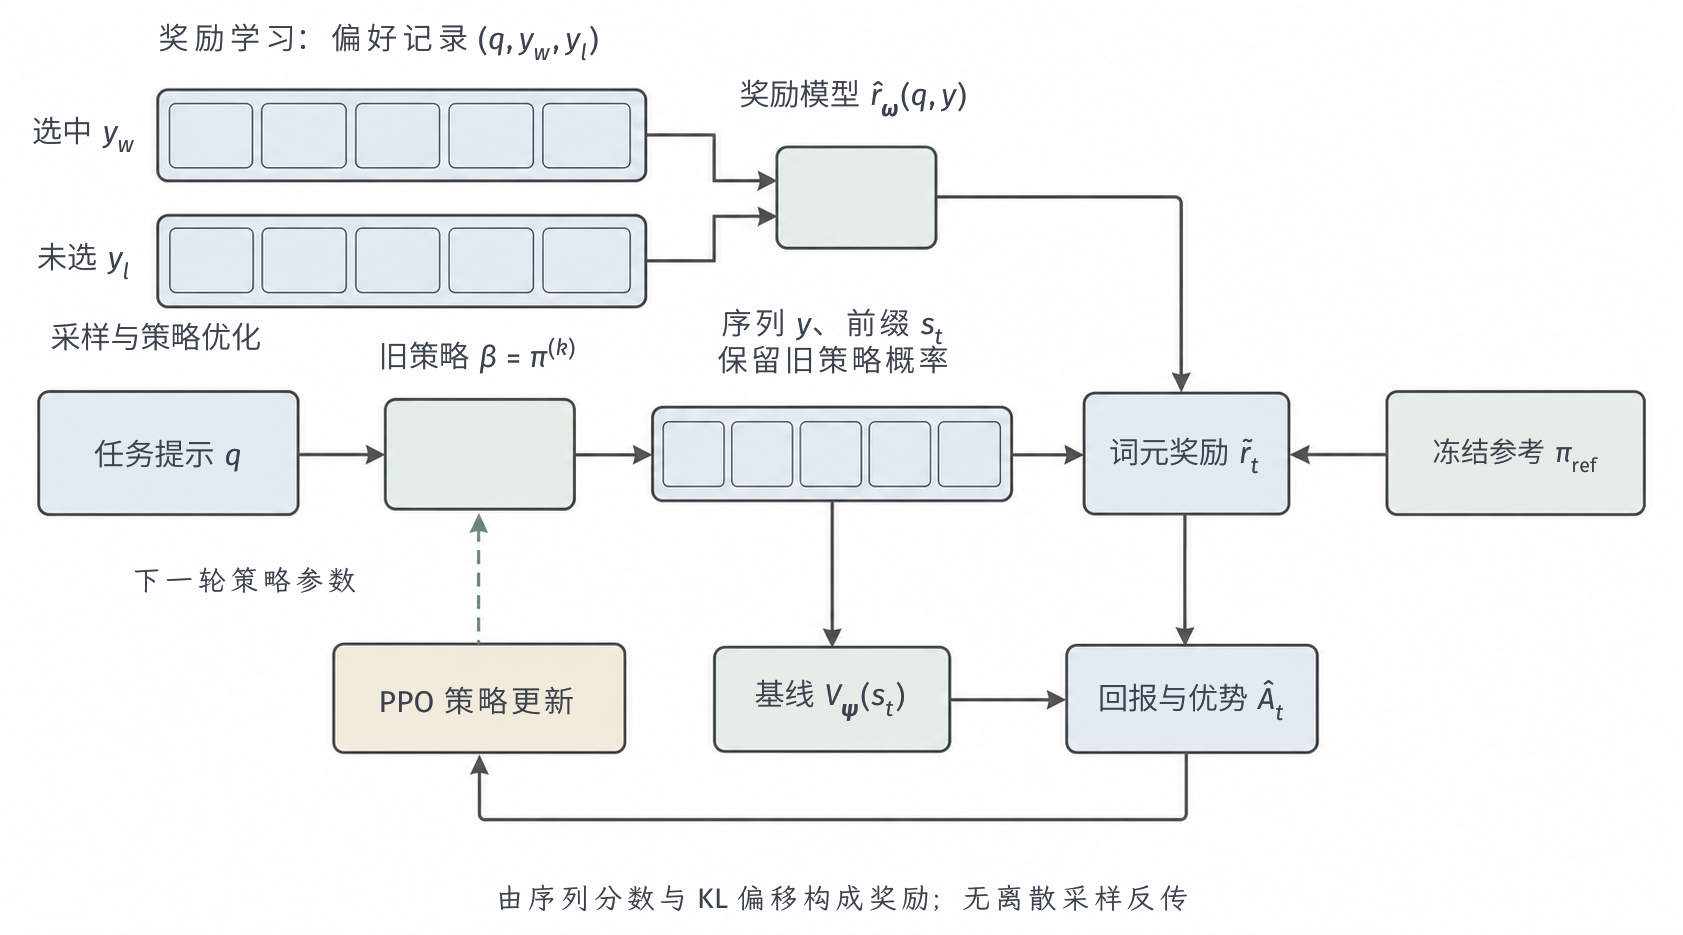
\includegraphics[width=157.400mm]{figures/10-reinforcement-learning/02-information-and-reward/generated/rl-reward-rlhf/figure.png}
  \caption{PPO式RLHF中的评价粒度。偏好标签训练完整回答评分器；旧策略逐token生成并记录采样概率，价值模型读取前缀提供基线。序列分数、旧策略概率与参考概率按式\eqref{eq:rl-reward-token-reward}构造逐token奖励，再经回报和优势估计进入策略更新；参考偏移不在更新器中重复计罚。图中连线表示回答、评分、采样概率及相应的训练信号，不表示通过离散采样端到端反向传播。图中省略部分批次字段连线：奖励模型评分仍读取本批$(q,y)$，PPO仍读取本批动作及旧策略概率。词元槽仅为示意，不规定回答长度。}
  \label{fig:rl-reward-rlhf}
\end{figure*}

逐token累加参考代价还会影响长短回答的权重。要把它与完整回答上的KL对应起来，可以使用序列概率分解所得的链式法则：
\[
  D_{\mathrm{KL}}(\pi(\cdot\mid q)\Vert\pi_{\mathrm{ref}}(\cdot\mid q))
  =\mathbb E_\pi\sum_{t<T}
    \log\frac{\pi(a_t\mid s_t)}{\pi_{\mathrm{ref}}(a_t\mid s_t)}.
\]
作为教学例，假设两个回答得分都为1，长度分别为2和4，各token的采样对数比恰好都是$0.1$。取$\lambda_{\mathrm{KL}}=0.5$，扣除参考代价后的样本分数分别为$0.9$和$0.8$。差异来自累加项，并不说明奖励模型明确偏好短回答；真实对数比也未必同号或恒定。若将KL或策略损失除以长度，就会改变长短回答的相对权重，而不是只做无影响的数值缩放。选择哪种聚合应依据任务标准，不能将一种归一化当成通用答案。

偏好标签不必都由人提供。Constitutional AI按照明确原则生成批评和修订，结合监督修订与AI偏好，再由AI偏好学习奖励、优化策略\scite{bai2022constitutional}
给定评分函数后，更换评价者不改变优化式的形式，却改变评分依据和误差来源，这些条件将在第~\ref{sec:rl-reward-sources}节检查。现在先固定奖励$r$，考察完整回答的概率分布如何在奖励与参考偏移之间取舍。下面在有限候选回答集合上优化全部概率分布，以便精确求解；实际网络只允许选择其参数可表示的分布，范围更小。

固定任务提示$q$，令$\mathcal Y$为有限非空的候选回答集合，$r(q,y)\in\mathbb R$，参考策略在每个候选上都满足$\pi_{\mathrm{ref}}(y\mid q)>0$，并取$\lambda_{\mathrm{KL}}>0$。在$\Delta(\mathcal Y)$上比较
\[
  F_q(\pi)=\mathbb E_{y\sim\pi(\cdot\mid q)}r(q,y)
   -\lambda_{\mathrm{KL}}D_{\mathrm{KL}}(\pi(\cdot\mid q)\Vert
                                    \pi_{\mathrm{ref}}(\cdot\mid q)).
\]
Gibbs变分结论表明，该目标的唯一最优分布是以参考概率为起点、按指数奖励重新加权：
\begin{equation}
  \begin{aligned}
    \pi^*(y\mid q)&=
      \frac{\pi_{\mathrm{ref}}(y\mid q)\exp(r(q,y)/\lambda_{\mathrm{KL}})}{Z(q)},\\
    Z(q)&=\sum_{z\in\mathcal Y}\pi_{\mathrm{ref}}(z\mid q)
                              \exp(r(q,z)/\lambda_{\mathrm{KL}}).
  \end{aligned}
  \label{eq:rl-reward-kl-optimum}
\end{equation}
有限集合、有限奖励与参考正支持保证$0<Z(q)<\infty$。这个结论把奖励差与最优策略相对参考策略的对数概率比联系起来，因而可用于随后将偏好拟合写成策略目标；它不保证参数化网络能够表示$\pi^*$。相关分布优化结论可参考\BookChapterRef{chap:information-theory-and-statistical-geometry}{卷2《数学准备：概率、因果与决策》的“概率分布的分析与优化”章}。

最优解并不把全部概率放在最高分回答上，而是以参考概率为起点，按$\exp(r/\lambda_{\mathrm{KL}})$重新加权。假设两个回答的参考概率都是$1/2$，奖励为$(\log3,0)$，$\lambda_{\mathrm{KL}}=1$，则$Z=2$，最优概率为$(3/4,1/4)$。若参考策略给某回答零概率，任何有限KL的策略也必须给它零概率，此时只能在参考支持内优化，不能沿用全回答空间的正支持结论。

从指数加权式取对数，得到$\log(\pi^*/\pi_{\mathrm{ref}})=r/\lambda_{\mathrm{KL}}-\log Z(q)$，于是奖励可写为“相对参考的对数概率”加$\lambda_{\mathrm{KL}}\log Z(q)$。后一个量对同一提示的所有回答相同。成对比较只需要奖励差，因此共同项恰好消去；这才使偏好拟合可以直接写成策略概率的目标，不是无条件地将奖励模型删掉。

这个精确解还提供了另一种偏好拟合方式。假定同一任务提示的偏好满足以$r$为效用的Bradley--Terry模型，便可把奖励差改写为最优策略相对参考策略的对数概率比差：
\begin{equation}
  \begin{aligned}
    r(q,y_{\mathrm w})-r(q,y_{\mathrm l})
    =\lambda_{\mathrm{KL}}\left[
      \log\frac{\pi^*(y_{\mathrm w}\mid q)}
                    {\pi_{\mathrm{ref}}(y_{\mathrm w}\mid q)}
      -\log\frac{\pi^*(y_{\mathrm l}\mid q)}
                    {\pi_{\mathrm{ref}}(y_{\mathrm l}\mid q)}
    \right].
  \end{aligned}
  \label{eq:rl-reward-dpo-change}
\end{equation}
其中$y_{\mathrm w}$和$y_{\mathrm l}$分别表示胜出和落选回答。同一任务提示的两边都有$\lambda_{\mathrm{KL}}\log Z(q)$，所以作差后消去；不同任务提示的归一化常数通常不能抵消。于是可以直接用策略概率比预测偏好，而不单独拟合奖励。以参数化策略替代$\pi^*$，将方括号内的量记为$z_{\bm{\theta}}(q,y_{\mathrm w},y_{\mathrm l})$，再最小化胜出标签的负对数似然，就得到\term{直接偏好优化}（direct preference optimization, DPO）：
\begin{equation}
  L_{\mathrm{DPO}}(\bm{\theta})
  =-\mathbb E_{(q,y_{\mathrm w},y_{\mathrm l})\sim\widehat P_{D_{\mathrm{pref}}}}
         \log\sigma\!\left(\lambda_{\mathrm{KL}} z_{\bm{\theta}}\right).
  \label{eq:rl-reward-dpo}
\end{equation}
期望在固定偏好记录$D_{\mathrm{pref}}$上计算，每条记录含同一任务提示及其胜出、落选回答。一次更新计算两条完整回答在当前策略和固定参考下的对数概率，再按式~\eqref{eq:rl-reward-dpo}下降；这个步骤既不采集新轨迹，也不训练显式价值模型。单条记录的梯度为
$-\lambda_{\mathrm{KL}}\sigma(-\lambda_{\mathrm{KL}} z_{\bm{\theta}})
[\nabla\log\pi_{\bm{\theta}}(y_{\mathrm w}\mid q)
-\nabla\log\pi_{\bm{\theta}}(y_{\mathrm l}\mid q)]$。
沿负梯度更新，局部方向提高胜出回答相对落选回答的对数概率。沿用均匀参考的双回答例，策略logit差就是$z$；当$z=0$且$\lambda_{\mathrm{KL}}=1$时，梯度为$-1/2$，以$0.2$为步长下降后$z=0.1$，胜出回答的概率约为$0.525$\scite{rafailov2023dpo}

DPO比较的是相对参考的变化，而非只看当前回答概率。另设两个回答的参考概率为$(0.8,0.2)$，当前概率为$(0.6,0.4)$，第一个是偏好标签中的胜者。两相对比为$0.75$和2，因此$z=\log(0.75)-\log2=\log(3/8)$。取$\lambda_{\mathrm{KL}}=1$，模型的胜出比较概率为$3/11\approx0.273$，即使当前第一个回答概率0.6仍高于第二个0.4。这个双回答例子说明偏好边际和动作概率是两个对象，更新关注相对参考提升了哪一个回答。

显式奖励模型加PPO，要给新采样回答评分并更新策略；标准DPO只在固定偏好比较记录上优化分类式损失。两者使用的训练记录和学习对象不同。上述换元解释了DPO与KL正则化最优策略的联系，却没有把DPO变成通常意义上的在线强化学习。实际模型类未必能表示$\pi^*$，有限记录未必覆盖所有回答，偏好也未必满足Bradley--Terry假设，所以不能由理想关系推出精确恢复最优策略。若在外层反复采样、标注再运行DPO，便形成迭代式偏好学习；在线访问和能区分候选奖励的新反馈来自外层协议，不来自分类损失本身。

% Outline: 5.2.5
\subsection{从过程与结果验证构造策略更新}
\label{sec:rl-reward-verification}

如果任务有明确的标准答案或可执行的产物，我们还可以绕开“逐对询问偏好”，直接检查候选是否满足某些条件：运行程序测试、按等价规则比对数学答案、或核对配送是否正确签收。这类检查可以反复使用同一标准，但它只能评价实际被检查到的那一个条件，不能因为几项检查通过就断言整个任务都已正确完成。

\begin{definition}[过程反馈与结果反馈]
  \label{def:rl-reward-verification}
  \term{结果反馈}（outcome feedback）评价行为结束后的产物或状态，例如答案是否等价、包裹是否正确签收。\term{过程反馈}（process feedback）评价中间状态、动作或步骤间关系，例如装载后身份是否一致、推导是否由前提合法推出。\term{可验证奖励}（verifiable reward）由明示验证规则产生；其可验证性依赖这条规则、检查时采用的前提和检查实现，不表示完整行为目标已经得到验证。
\end{definition}

过程与结果提供的证据也不能相互替代。推导可能使用非法除法却偶然得到正确答案，所以结果通过不足以证明过程有效；反过来，每步合法的变换也可能只是在反复改写题目，没有回答问题。表~\ref{tab:rl-reward-verifiers}据检查对象和前提比较验证器，自动检查是否可信仍要逐项判断。

\begin{table*}[htbp]
  \centering\small
  \begin{tabularx}{\linewidth}{@{}>{\raggedright\arraybackslash}p{21mm}*{4}{>{\raggedright\arraybackslash}X}@{}}
    \toprule
    检查器 & 可检查对象 & 检查前提 & 反馈粒度 & 主要漏检 \\
    \midrule
    规则验证器 & 格式、身份、答案等价 & 解析与等价规则符合标准 & 字段、步骤、结果 & 格式正确但内容错误；解析漏洞 \\
    执行器 & 代码、操作的实际结果 & 沙箱、程序测试用例、执行环境有效 & 工具调用或整次运行 & 未执行的程序测试用例、超时与资源副作用 \\
    形式检查器 & 形式命题及证明 & 形式化忠实，公理和检查内核可信 & 推理步骤、完整证明 & 证明了错误形式化的命题 \\
    模型评判器 & 开放式内容与解释 & 训练覆盖、提示及标准适用 & 片段、回答 & 风格偏好、位置偏差、共同模型盲点 \\
    \bottomrule
  \end{tabularx}
  \caption{四种验证器实际检查的对象及漏检范围。执行测试只支持所执行的程序测试用例，形式检查只支持所形式化的命题；两者都不能自行证明完整需求已被正确检查。}
  \label{tab:rl-reward-verifiers}
\end{table*}

拿到候选的验证得分后，可以比较同一任务提示下多个回答，为策略提供相对信号。\term{组相对策略优化}（group relative policy optimization, GRPO）以这组回答的得分为基准，给高于组均值的回答正信号，给低于均值的回答负信号，从而不必另拟合价值基线。沿用有限序列的未折扣评价，令旧策略$\beta$对$q$独立采样$m$个回答$y_i$，其验证或奖励模型得分记为$v_i$；这里$i$编号候选，不是$r_t$中的动作时刻。为中心化得分并统一组内尺度，定义
\begin{equation}
  \bar v=\frac1m\sum_{i=1}^m v_i,\qquad
  s_v=\sqrt{\frac1m\sum_{i=1}^m(v_i-\bar v)^2},\qquad
  \widehat A_i=\frac{v_i-\bar v}{s_v+\epsilon_{\mathrm{num}}},
  \label{eq:rl-reward-grpo-advantage}
\end{equation}
标准差使用分母$m$，$\epsilon_{\mathrm{num}}>0$防止分母为零。结果监督时，同一个$\widehat A_i$可以用于回答$i$的全部token，但它只表示该回答相对本组得分的高低，既不是逐token标签，也不是对状态价值函数的估计。

若两个回答都先完成相同的身份核对，随后一个正确装载、另一个拿错包裹，终局得分可以分别为1和0。组内信号会给第一条完整回答正值、第二条负值，连共同的核对步骤也使用不同符号。它适合推动完整行为概率，却不能据此判断核对在第二条轨迹中是错误动作；要作这种局部判断，仍需过程证据或有依据的归因。

为了将这个组信号接入策略更新，令$T_i$为回答长度，$\varrho_{i,t}=\pi_{\bm{\theta}}(y_{i,t}\mid q,y_{i,<t})/
\beta(y_{i,t}\mid q,y_{i,<t})$为当前与旧策略的token概率比，$\ell_{i,t}^{\mathrm{clip}}$为式~\eqref{eq:rl-reward-ppo}中以$\widehat A_i$替代$\widehat A_t$的剪裁项。一个常见实现先在每个回答内平均token项，再在组内平均，并扣除参考偏移代价，最大化代理目标
\begin{equation}
  \widehat{\mathcal L}_{\mathrm{GRPO}}
  =\frac1m\sum_{i=1}^m\frac1{T_i}
      \sum_{t=0}^{T_i-1}
       \left(\ell_{i,t}^{\mathrm{clip}}-\lambda_{\mathrm{KL}} k_{i,t}\right),
  \label{eq:rl-reward-grpo}
\end{equation}
其中$k_{i,t}$是所选参考KL估计或局部近似，常用形式为
$k=\exp(-\ell)+\ell-1$，$\ell=\log(\pi_{\bm{\theta}}/\pi_{\mathrm{ref}})$；
若当前策略和参考策略在同一合法token集合上都为正，且动作由$\pi_{\bm{\theta}}$采样，那么给定前缀有$\mathbb E_{\pi_{\bm{\theta}}}\exp(-\ell)=1$，从而$k$的期望等于前向KL。旧策略采样不自动满足这个分布条件；复用旧样本时若没有分布校正，样本平均就不能当成精确KL，更不能证明硬约束成立。长度平均、剪裁和采样KL都属于代理目标的选择，与无近似的期望奖励梯度需要区分。

GRPO中选用的$k$还区分了样本值与期望值。普通对数比$\ell$可以为负；而$e^{-\ell}\geq1-\ell$给出$e^{-\ell}+\ell-1\geq0$，所以这种样本项每次都非负。它的KL含义仍依赖正确的动作抽样分布，非负并不使旧策略样本平均自动成为当前策略的精确KL。计算形式与概率依据需要分别检查。

\begin{example}[一组验证得分的更新信号]
  \label{ex:rl-reward-grpo}
  假设$m=4$，四个得分为$(1,1,0,0)$，则$\bar v=0.5$、$s_v=0.5$。忽略极小稳定项，相对信号为$(1,1,-1,-1)$。为计算一次更新，再设任务只有一步和两个动作，成功动作概率为$p=\sigma(z)$，当前$z=0$，不加KL惩罚，概率比处在未剪裁区。这组样本对logit的梯度为
  \[
    \frac14\{2(1)(1-p)+2(-1)(-p)\}=\frac12.
  \]
  用$0.2$为步长上升，得到$z'=0.1$，成功动作概率约为$0.525$。若整组全为1或全为0，中心化后的分子都为0；稳定项只能使计算有限，不能产生奖励梯度。若实现保留KL项，正则化仍可能产生梯度。
\end{example}

标准化还改变不同结果的相对幅度。若四个分数为$(1,0,0,0)$，均值为$1/4$，标准差为$\sqrt3/4$；忽略数值稳定项，成功样本信号为$\sqrt3$，三个失败样本各为$-1/\sqrt3$。这与前面两个成功、两个失败时的$\pm1$不同。更大幅度来自本组成功比例较低，并不表示检查器证明这次成功更重要或各步骤贡献更大。

上述算例给出的是组内相对信号，不能直接当作无偏真实优势。即使不除以标准差，组均值含样本自身也会改变梯度期望。为了看清这一点，固定$q$和得分函数$v$，从$\pi$独立同分布采样，记$\bm g_i=\nabla\log\pi(y_i\mid q)$。利用$\mathbb E\bm g_i=0$，可得
\[
  \mathbb E\left[\frac1m\sum_i(v_i-\bar v)\bm g_i\right]
  =\left(1-\frac1m\right)\nabla\mathbb E_\pi v.
\]
缩放因子来自$\bar v$中与$\bm g_i$相关的自身得分，其余独立样本的交叉期望为零。再除以随机$s_v$，还会引入与组内成功比例有关的权重；二值奖励混合组中，较少见结果的标准化绝对值更大。改用不含自身的组均值可以消除这个特定缩放，但不能同时消除标准化、剪裁或复用旧样本造成的偏差。

“组均值作基线”与前章动作前固定基线的条件不同：这份均值包含正在被加权样本的自身得分，因而与其概率梯度相关。独立的其他回答部分会在期望中抵消，自身那一份却扣掉了$1/m$的梯度；所以即使只中心化也会出现上面的缩放。数值稳定或每项非负并不修复这种统计依赖，重复使用旧策略样本还要另查分布校正。

组内比较只要求给出$v_i$，并未规定它必须来自规则。DeepSeekMath提出GRPO，并讨论结果奖励模型、过程奖励模型和迭代刷新，反馈并不限于规则判分\scite{rl5-shao2024deepseekmath}
DeepSeek-R1原始技术报告中的R1-Zero及R1推理训练使用正确性、格式等规则奖励；但R1完整多阶段流程还包含监督微调及用于通用任务回答的模型奖励，不能用推理阶段的反馈概括全部训练\scite{deepseek2025r1}

\term{基于可验证奖励的强化学习}（reinforcement learning with verifiable rewards, RLVR）说明奖励由明示规则产生，GRPO则说明拿到分数后如何更新策略，两者不是同一个分类依据。验证器将未满足条件的候选判为通过，称为假阳性（false positive）；解析偏差、测试泄漏或长度与表达偏好也可能被策略用来增加得分。增加同一任务提示的采样数可提供更多组内比较，却不会补齐未检查要求。在多轮工具任务中，还要明确评分针对动作格式、工具执行还是最终完成情况；将终局成功平均分给工具调用，并没有取得独立的动作正确性标签。更长交互的前沿问题见第~\ref{chap:rl-overview}章，语言模型实现由应用卷承接。

% Outline: 5.2.6
\subsection{反馈来源与目标可识别性}
\label{sec:rl-reward-sources}

回到配送任务，已有示范可能足以复现动作，偏好记录可能足以预测路线胜负，验证器可能足以判断签收身份。要判断目标是否可识别，必须先指定想要哪种结论，再检查产生同样反馈的候选解释是否都支持它。奖励即使不唯一，候选奖励也可能一致支持当前动作；偏好即使预测准确，也不能说明未被评价的要求已经学会。这正是前章可识别性在目标反馈上的应用。

同一对行为的胜负标签可以由人判断，也可以由模型判断。比较这两种来源，主要要检查判断依据、成本和误差是否相同，而不是仅比较记录格式。形式相同不意味着评价质量相同。

\term{基于AI反馈的强化学习}（reinforcement learning from AI feedback, RLAIF）由AI承担部分评价，再用所得反馈学习策略。\term{原则指导反馈}（constitutional feedback）则以明确原则指导评价或修订，用这些原则产生批评、修订示范或偏好。前者说明评价来源，后者说明判断依据；原则不是与示范、偏好互斥的记录类型，其选择仍须由外部目标约定。

\begin{table*}[t]
  \centering\small
  \begin{tabularx}{\linewidth}{@{}>{\raggedright\arraybackslash}p{22mm}*{5}{>{\raggedright\arraybackslash}X}@{}}
    \toprule
    来源或协议 & 判断依据 & 相关偏差 & 可追溯性 & 查询成本 & 外部校验 \\
    \midrule
    人类反馈 & 任务知识、个人偏好、指南 & 疲劳、群体差异、顺序效应 & 需保留指南与标注群体 & 人工时间 & 交叉复核、真实结果 \\
    RLAIF & AI知识与提示中的标准 & 共享训练偏差、风格偏好 & 需记录模型和提示版本 & 推理及抽查成本 & 独立人评、规则或执行 \\
    原则指导反馈 & 显式原则及其解释 & 原则遗漏、冲突解释 & 原则可见不等于执行透明 & 原则维护与评价成本 & 逐原则反例测试 \\
    模型评判器 & 学得评分或比较函数 & 分布外失准、位置与长度偏差 & 需记录反馈模型的训练样本组成及模型版本 & 批量打分与刷新 & 留出来源、实物或程序检查 \\
    \bottomrule
  \end{tabularx}
  \caption{反馈来源及协议的判断依据、成本与校验方式。RLAIF可使用原则指导的模型评判器，因此同一系统可以同时属于多行，不能按互斥类别解读。}
  \label{tab:rl-reward-sources}
\end{table*}

假设人工标注员和模型都只看终点照片，两者都判断“已送达”，却都看不到包裹内部破损。增加来源一致性没有增加包裹内部破损的检查记录，因此不能推出包裹完好。来源分歧也未必是噪声：一位收件人看重速度，另一位看重省电，可能确实采用不同取舍，不应直接删除其中一方的反馈。

表~\ref{tab:rl-reward-sources}列出的外部校验，也应注明被评价行为的任务条件和适用范围。评价器只在身份、路线条件等必要字段齐全的短距离配送记录上检查过，就不能直接用于长路线、身份缺失或新包裹，并声称同样可靠。现有证据只支持已检验策略在这些配送条件和评价标准下的结论；要判断多个奖励解释是否会造成实际失配，还要比较未见行为上的排序。

% Outline: 5.3
\section{奖励归因受限下的强化学习}
\label{sec:rl-reward-credit}

假设我们已经约定了“配送成功”的确切含义、也能拿到可靠的终局反馈，剩下的问题是：怎样用这一个结果去更新核对、装载等早期动作。此时目标与反馈语义都已固定，但结果回溯、过程判断、奖励变换和辅助目标这几种做法改变的学习对象并不相同：有的需要新增步骤标签或专家评价，有的只是改变记账方式或训练安排；它们能否保持原目标，所要求的条件也各不相同。

% Outline: 5.3.1
\subsection{基于长期结果回溯构造局部学习信号}
\label{sec:rl-reward-redistribution}

在四步配送中，早期核对决定是否拿对包裹，中间搬运可能只是执行既定方案。REINFORCE或多步回报能将终局成功用于核对动作的更新，但搬运和提示播放也可能收到同一个成功回报。前章的基线和自举分别减少共同波动、缩短传播路径，并没有直接测量“改变这个动作会使结果变化多少”。这里回用第~\ref{chap:rl-learning}章的估计方法，进一步检查局部信号所表达的贡献。

\term{奖励重分配}（reward redistribution）将同一结果重新记到轨迹上的不同位置，使结果与关键事件的时间联系更短。要判断这种记账是否仍优化原目标，必须按原来的折扣权重比较整条轨迹的新旧奖励，而不能只比较未折扣总和。若要求逐轨迹保持回报，应满足
\begin{equation}
  \sum_{t=0}^{H-1}\gamma^t\widetilde r_t
    =\sum_{t=0}^{H-1}\gamma^t r_t.
  \label{eq:rl-reward-redistribution}
\end{equation}
逐轨迹相等足以保持每个策略的期望回报；也可以使用较弱条件，但需要期望相等对全部待比较策略成立。另要检查信号何时可得。依赖整段历史的新奖励通常不是原状态上的马尔可夫奖励，需要相应表示；若它依赖记账时刻之后才发生的结果，只加入过去历史仍不能使反馈当时可得。

例如$H=4$、$\gamma=0.9$，原奖励$(0,0,0,1)$对应初始回报$0.9^3=0.729$。若全部移至$t=0$，新奖励应为$(0.729,0,0,0)$；若移至$t=1$，则应为$(0,0.81,0,0)$，两者按折扣计算仍为$0.729$。直接移成$(1,0,0,0)$只保留未折扣总和，没有保留原目标。若轨迹长度可变，同样忽略折扣还会改变快慢路径的排序。

保持总回报也不意味着可以直接用新奖励计算reward-to-go，即从当前动作起的后续奖励回报，包含该动作的奖励。假设终局成败取决于最后一个动作，却将全部结果事后记到$t=0$，末步的局部回报就变为0，用它更新末步策略会丢掉该动作的影响。第~\ref{chap:rl-learning}章之所以能删去过去奖励，是因为过去结果不受当前动作影响；事后前移的信号不满足这个因果条件。将不变的完整轨迹回报与整条轨迹的对数概率梯度相乘，仍保留原目标梯度。要改用局部更新，还须另外证明重分配与估计器的配套条件。

这个失效可用四步任务的最后一次交付手算。前面三步固定，末步选择正确收件人的概率为$p=\sigma(\theta)$，成功得1、失败得0，$\gamma=0.9$。原起点目标是$J=0.729p$，导数为$0.729p(1-p)$。若事后把成功分全部记成$t=0$的$0.729$，总目标仍相同，但末步之后的重分配回报为0；用它乘末步对数概率梯度会给出零更新。完整轨迹回报仍含末步结果，乘它的对数概率梯度才能保留原导数。过去奖励可被删去所需的因果条件，不能只由总和相等推出。

一种重分配依据是观测、动作前缀对最终回报预测的影响。令$m_t$预测看到前缀后的最终回报，将$m_t-m_{t-1}$视为读入新一步记录后的回报预测增量；取$m_{-1}=0$且$m_{H-1}=G_0$，相邻差求和恰为$G_0$。若将其记为折扣局部奖励，且$0<\gamma\leq1$，可取$\widetilde r_t=\gamma^{-t}(m_t-m_{t-1})$以抵消记账位置的折扣。末端预测不等于真实回报时必须补残差，否则总回报也改变了。实际学习还需控制预测误差和$\gamma^{-t}$的放大；RUDDER用回报预测与贡献分析构造信号，其机制入口已在第~\ref{chap:rl-learning}章介绍。

回报预测增量仍不等于改变动作所产生的干预贡献。假设正确核对后屏幕总会闪光，日志中闪光与成功高度相关；但关闭闪光不会改变交付，拿错包裹才会导致失败。归因模型只依据相关性时，可能把奖励分给闪光。检验应改变无关标记、受控比较关键动作，并观察实际交付结果；仅有回报预测误差下降不足以证明贡献判断正确。对动作干预作比较，还要固定动作前的共同条件，说明允许的干预及其后续执行规则，并检验支持与相应的混杂控制条件；单纯的预测增量没有提供这些条件。这个区分用于判断局部奖励信号能否解释动作贡献，可参考\BookChapterRef{chap:causal-inference}{卷2《数学准备：概率、因果与决策》中讨论因果响应的章节}。

% Outline: 5.3.2
\subsection{基于过程反馈构造局部学习信号}
\label{sec:rl-reward-process}

若终局日志无法区分核对错误与中途换包，可以新增装载前的身份检查。这个检查提供新的中间证据，而不是将原总分分摊到各步。需要先明确它评价什么：读码动作、装载后的身份关系和到达时的包裹状态对应不同决策，只有步骤边界和被检关系清楚，才能确定反馈监督的对象。

图~\ref{fig:rl-reward-process}把人工标注、规则检查、执行记录和模型步骤评价放到同一轨迹中，标明各自覆盖的步骤。例如执行记录只证明包裹放入箱内，不证明身份正确；模型觉得搬运平稳，也不能替代破损检查。推理任务中的逐步骤评价同样需要明确标签标准及标注范围。

在Lightman等的工作中，标注者按统一规范把数学解答的步骤判为正、负或中性。带标签的解答前缀成为训练样本，\term{过程奖励模型}（process reward model, PRM）学习在题目和已生成前缀给定时预测这三类标签的概率。训练对象是这个评价模型：只对已有步骤标签拟合分类概率，未被评价的步骤不能自动补成正例。模型预测的步骤分数还须聚合，才能比较两份完整解答\scite{lightman2023verify}。

过程奖励模型预测的是评价者会怎样判断当前步骤；价值模型预测的是该前缀之后的累计回报。一步被判合法，不表示后来一定解对题目，也不直接给出这步相对其他动作的优势。要将这些分类概率用于整解排序或训练，需要另选聚合规则，并说明它对应什么问题。

设题目为$q$，一份候选解为$c=(c_1,\ldots,c_m)$，$m$是其步骤数。按该论文的主要评分约定，将中性与正类合并；令$p_j$为模型根据$(q,c_{1:j})$预测第$j$步属于这两类的概率，整解排序分数为
\begin{equation}
  F_{\mathrm{PRM}}(q,c)=\prod_{j=1}^{m}p_j.
  \label{eq:rl-reward-prm-score}
\end{equation}
例如两份两步解的预测概率分别为$(0.9,0.9)$和$(0.99,0.6)$，分数为$0.81$与$0.594$，会选择前者。这个乘积是评价模型的排序规则，不能仅凭相乘就解释为全部步骤正确的真实联合概率；步骤较多时，乘积也可能因长度而降低。原文还比较了取最小步骤分数及不同中性处理的选择，它们改变的是整解排序方式，不是环境奖励的测量规则。

即使每步概率都准确，乘积也未必是全部正确的概率。设两步同时依赖一个共同前提，前提以$0.9$概率有效；有效时两步都正确，无效时两步都错误。两步各自正确概率都是$0.9$，共同正确概率却是$0.9$而非$0.81$。概率链式法则需要逐步条件于此前步骤都正确；一般PRM的步骤预测没有自动提供这种条件量。因此乘积可作排序规则，不能仅因每项像概率就认作真实联合成功率。

在候选筛选评价中，生成器保持固定，对每道测试题采样$n$份完整解，再交付$F_{\mathrm{PRM}}$最高的一份，这就是best-of-$n$选择。它既要支付$n$次生成成本，也要评价这些候选的步骤；报告选择效果时必须固定生成器、采样预算和测试范围。该论文的主要比较按最终答案检查被选解的成功率，支持的是这一筛选用途，不能直接写成策略梯度训练带来的收益。若随后用步骤分数更新生成策略，还须另行规定采样策略、局部归因和优化目标；步骤判断概率本身不是状态价值或真实优势，过程奖励模型也没有普遍优于结果奖励模型的保证。

即使各处检查都通过，局部正确也可能没有组成全局成功。机器人每次搬运都遵守速度限制、每次放置都平稳，却只在两个中间站往返，没有交给收件人。过程条件没有覆盖最终交付；若各次身份检查只看单个字段，还可能遗漏跨步骤身份一致性。因此，将局部分数求和之前要解释它与整体要求的关系，终局检查不能仅因步骤有标准就取消。

过程反馈也增加获取和维护成本：标注量通常随步骤数增长，不同标注者还可能采用不同的步骤切分。模型反馈若有系统偏差，会在多个位置重复传入更新。可以比较只补关键步骤与标注全部步骤所需成本，统一标准版本，再检查独立交付结果是否改善。若发现检查标准遗漏了要求，就需要修订目标标准，不能只调整局部信号权重。

\begin{figure*}[htbp]
  \centering
  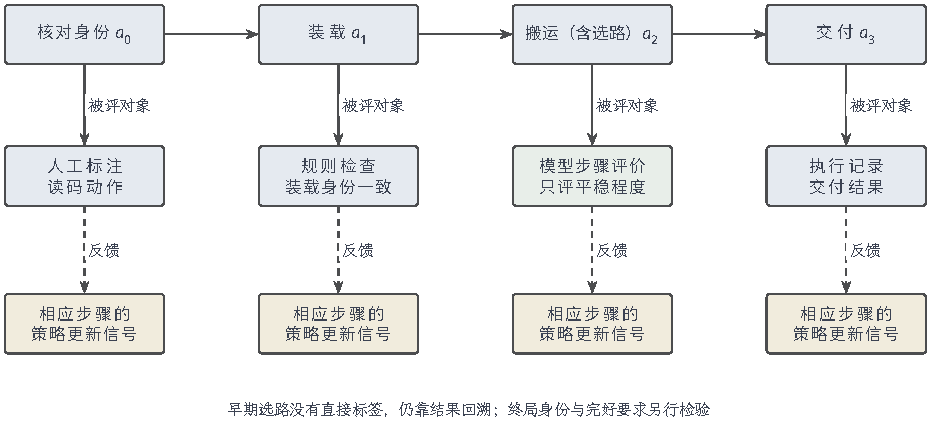
\includegraphics[width=157.618mm]{figures/10-reinforcement-learning/02-information-and-reward/tikz/rl-reward-process.pdf}
  \caption{过程反馈缩短部分决策到评价的路径。上方为按时间执行的配送步骤，下方为评价来源；由反馈指向更新对象的虚线表示学习信号。未标注步骤仍依赖终局回报传播，局部通过不取代最终身份和完好检查。}
  \label{fig:rl-reward-process}
\end{figure*}

% Outline: 5.3.3
\subsection{基于奖励变换构造局部学习信号}
\label{sec:rl-reward-shaping}

即使不增加任何新检查，也可以依据已有目标人为构造更即时的引导信号。例如希望鼓励机器人靠近终点，但简单地“只要靠近就加分”会被钻空子——机器人可以反复离开再靠近、不断领分。要避免附加分数任意改变长期目标，可以采用\term{潜势型奖励塑形}（potential-based reward shaping）：先给每个状态打一个“潜力分”，再只按与任务相同折扣的相邻潜力之差发附加奖励，使一段路途上的附加项能够逐项抵消。

\begin{definition}[潜势型塑形]
  \label{def:rl-reward-shaping}
  给定与任务相同的折扣$\gamma$及状态势函数$\Phi:S\to\mathbb R$，定义
  \[
    F(s,a,s')=\gamma\Phi(s')-\Phi(s),\qquad
    r'_t=r_t+\gamma\Phi(s_{t+1})-\Phi(s_t).
  \]
  $\Phi$是人为指定或从交互训练记录学习的状态评分，称为势函数；附加奖励必须采用这个折扣差形式，不能用任意启发式分数替代。
\end{definition}

折扣差为什么能避免给往返反复加分，可以先看两步。令起点势为0、近处势为1，$\gamma=0.9$；从起点到近处的附加奖励为$0.9$，再回起点为$-1$，折扣后的附加总和为$0.9+0.9(-1)=0$。只奖励靠近而不扣离开，会使同样往返拿到额外分。势差把同一中间状态在相邻两步中的贡献抵消，下面的推导把这个计算推广到整个轨迹并保留末端项。

为判断附加信号是否仍评价原任务，我们比较塑形前后的完整折扣回报。下面利用相邻势项相消，证明在给定条件下两者只差一个不依赖策略的期望常数；这是策略不变奖励变换的经典结论\scite{rl5-ng1999shaping}

\begin{theorem}[无限折扣时域的塑形不变性]
  \label{thm:rl-reward-shaping}
  设$0\leq\gamma<1$，固定所有待比较策略共同使用的有界可测状态势函数$\Phi:S\to\mathbb R$及初始分布$\mu_0$。假设各策略的原折扣回报作为随机级数几乎处处收敛，且所得实随机变量可积。则塑形后的回报几乎处处满足
  \[
    G'_0=G_0-\Phi(s_0),\qquad
    J'(\pi)=J(\pi)-\mathbb E_{\mu_0}\Phi(s_0).
  \]
  因而所有策略在标准期望折扣回报下的排序不变。
\end{theorem}

\begin{proof}
  先取长度为$H$的有限前缀，以便保留末端边界项。将塑形奖励代入折扣和，相邻势项逐项相消：
  \begin{align*}
    \sum_{t=0}^{H-1}\gamma^t r'_t
    &=\sum_{t=0}^{H-1}\gamma^t r_t
       +\sum_{t=0}^{H-1}
          \bigl[\gamma^{t+1}\Phi(s_{t+1})
                          -\gamma^t\Phi(s_t)\bigr]\\
    &=\sum_{t=0}^{H-1}\gamma^t r_t
       -\Phi(s_0)+\gamma^H\Phi(s_H).
  \end{align*}
  由$|\Phi(s)|\leq M$，末端项绝对值至多为$\gamma^H M$，当$H$趋于无穷时消失；若$\gamma=0$，从$H\geq1$起该项就为零。因此在原折扣级数收敛的轨迹上满足$G'_0=G_0-\Phi(s_0)$。势的有界性保证差值可积，取期望得到只依赖共同初始分布的偏移。任意两策略减去同一个期望数值，其回报差和排序均不变。
\end{proof}

保持期望排序不要求$\Phi$等于精确价值。即使势函数误将慢路线评为接近终点，只要有界且按同一折扣差加入，定理仍成立；但错误势值可能妨碍学习，使速度或有限样本回报变差。若初始状态随机，$-\Phi(s_0)$也是随机偏移，可能改变方差及\term{条件风险价值}（conditional value-at-risk, CVaR）这类尾部评价。以损失$-G_0$定义CVaR时，它评价上尾的大损失，对应回报较差的结果。第~\ref{chap:rl-trustworthy}章的风险目标需要另查不变性，不能继承这里的期望结论。

有限任务没有无穷尾项可供消去，必须保留终端势。允许势随时刻变化，采用
$r'_t=r_t+\gamma\Phi_{t+1}(s_{t+1})-\Phi_t(s_t)$。
沿相同方式展开，可得
\begin{equation}
  \sum_{t=0}^{H-1}\gamma^t r'_t
  =\sum_{t=0}^{H-1}\gamma^t r_t
      -\Phi_0(s_0)+\gamma^H\Phi_H(s_H).
  \label{eq:rl-reward-shaping-terminal}
\end{equation}
这个恒等式也适用于有限时域的$\gamma=1$。令$\Phi_H=0$足以消去末端项；若$H$固定，终端势为所有策略共享的常数也能保持排序。$\gamma=0$时末端项不影响目标，但其他折扣下必须显式处理边界。

自然终止和采样时间截断对应不同边界。自然终止后不再记账时，应将终止势设为零，或显式抵消$\gamma^T\Phi_T(s_T)$；若$T$可变且$\gamma<1$，即便终端势都是同一非零常数，折扣后的末端项也会随长度变化。若采用吸收状态并无限继续记塑形奖励，尾项可以继续相消，但不能只记进入吸收状态的一步，省略随后塑形项。训练批次截断则可能尚未结束任务，需要保留原续接价值和对应塑形价值$V'(s)=V(s)-\Phi(s)$；若不保留，就要明示改求有限时域目标。未计算续接价值不意味着它为零。

\begin{example}[遗漏终端势会改变排序]
  \label{ex:rl-reward-terminal}
  假设$H=1$、$\gamma=0.9$，从同一起点选择到终点甲或乙，原奖励都是0，且$\Phi_0(s_0)=0$。若$\Phi_1(\text{甲})=1$、$\Phi_1(\text{乙})=0$，到达后立即停止记账，新回报分别为$0.9$和0，原本并列的路径变成甲更优。将两个终端势都设为0则消除了这一差异；在含中间步骤的任务中，即使中间势不准确，只要满足相应定理条件，仍可保持期望排序。
\end{example}

现在可以具体区分这些保持条件。潜势塑形使共同起点的回报只差固定势值，重分配可以要求逐轨迹折扣回报完全相同，一般辅助奖励则不自动具有这两种性质。即使附加信号更密集、代数上保持了目标，也没有证明它等于动作的因果贡献。

% Outline: 5.3.4
\subsection{基于辅助目标构造局部学习信号}
\label{sec:rl-reward-auxiliary}

“给学习增加辅助信号”有两种作用位置完全不同的做法，必须分清。让机器人预测下一时刻的位置，是用预测误差训练状态表示，促使它保留用于后继预测的特征，行为最终仍按原任务回报评价；而为“每次到达装载区”加分，则是直接改变了策略优化的回报。两者都可能改变学习速度，但前者作用于表示、后者作用于计分，并非等价。是否更快达到同一原任务回报，或是否改善原任务，还需在相同采样与计算预算下分别检验。

为说明更新位置，设共享表示参数为$\bm{\eta}$，任务的策略或价值损失为$L_{\mathrm{task}}$，下一状态预测损失为$L_{\mathrm{aux}}$。以$\lambda$设置辅助损失权重、$\alpha$为步长，联合更新为
$\bm{\eta}^{(k+1)}=\bm{\eta}^{(k)}
-\alpha\nabla_{\bm{\eta}}(L_{\mathrm{task}}+\lambda L_{\mathrm{aux}})$。
辅助预测梯度改变共享表示，最终行为仍按原任务回报评价。若改为给动作增加辅助奖励$b_t$，采用$r'_t=r_t+\lambda b_t$，则优化目标变为
$J'(\pi)=J(\pi)+\lambda\mathbb E_\pi\sum_t\gamma^t b_t$，
除非$b_t$满足额外不变条件，这个新目标不再等于原任务。图~\ref{fig:rl-reward-auxiliary}将两条路径分别接到共享表示和回报，显示它们改变的对象。

\begin{figure*}[htbp]
  \centering
  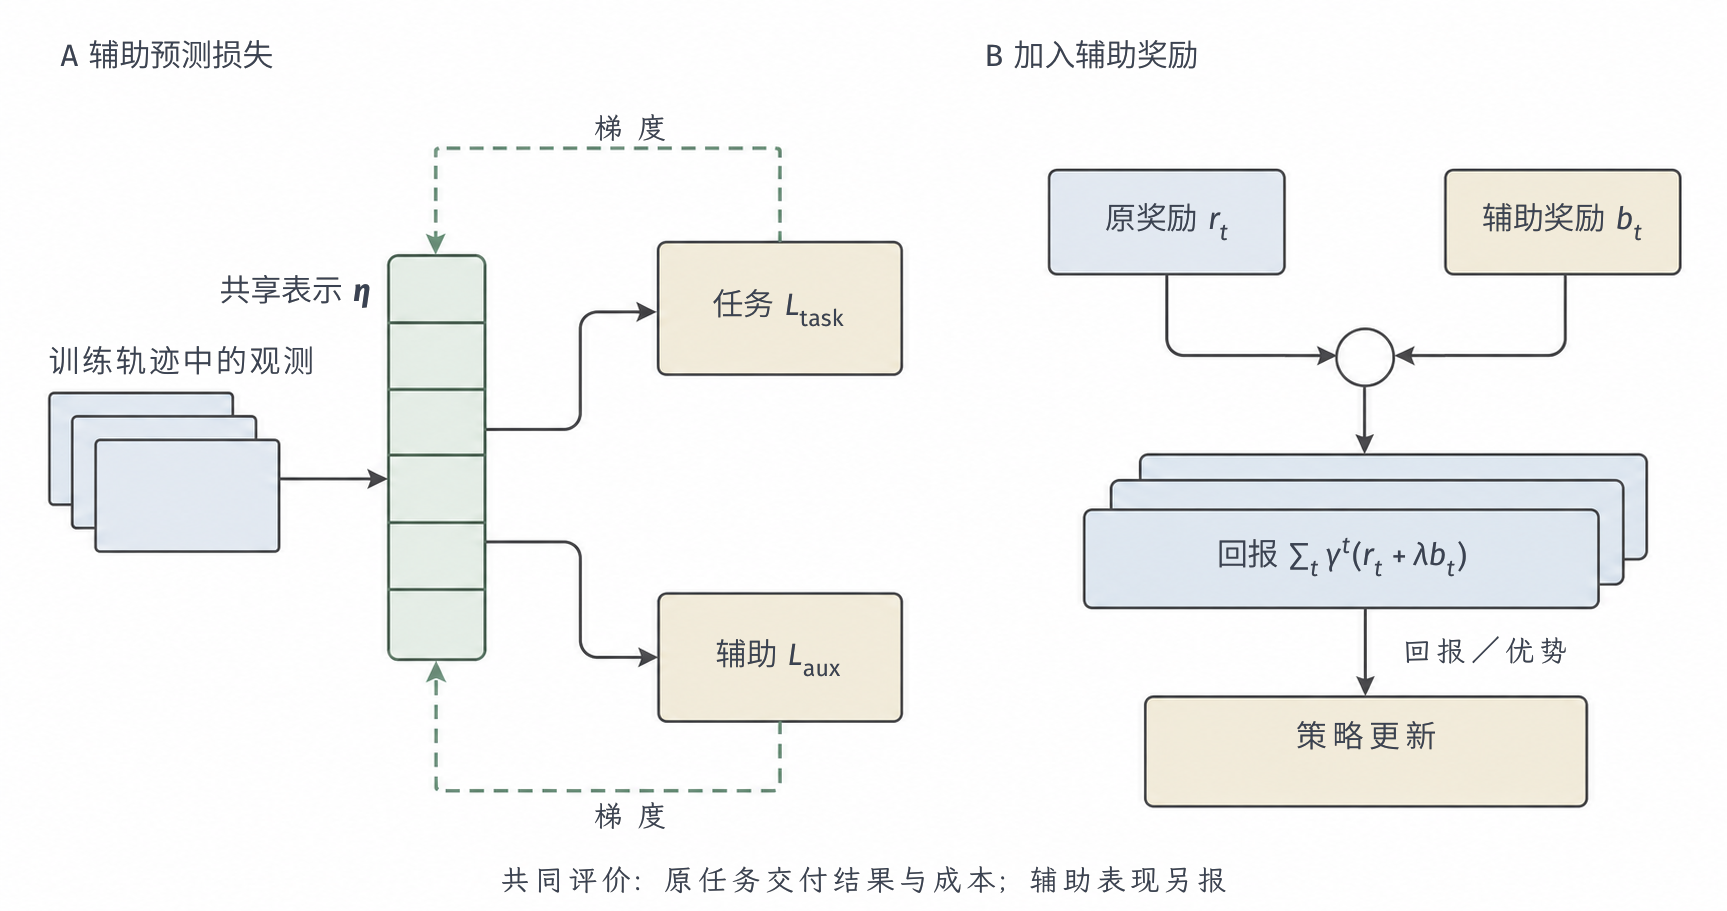
\includegraphics[width=157.400mm]{figures/10-reinforcement-learning/02-information-and-reward/generated/rl-reward-auxiliary/figure.png}
  \caption{辅助预测损失与辅助奖励的干预位置。左侧虚线为损失对共享表示的梯度；右侧辅助奖励先进入回报，再产生策略更新信号。两种训练的最终行为都应按未掺入辅助分数的原任务标准评价。帧、特征格与回报条带数量仅为示意。}
  \label{fig:rl-reward-auxiliary}
\end{figure*}

辅助梯度也可能与任务梯度冲突。用一个标量参数作教学例，令$L_{\mathrm{task}}=(\eta-1)^2/2$、$L_{\mathrm{aux}}=(\eta+1)^2/2$。在$\eta=0$，两梯度为$-1$与1；若辅助权重为1，合成梯度为0，尽管任务损失尚未最小。这个例子不说明所有辅助预测都会妨碍学习，而是说明共享参数和增加监督，并没有自动保证任务优化方向得到改善。

另外两种训练安排也需区分。训练课程改变任务分布，例如先练短路线，再增加距离；人为子目标改变决策组织，例如先到装载区，再去收件处。二者都不必增加奖励，也不等于潜势塑形。时间抽象回用第~\ref{chap:rl-learning}章；目标重标记及\term{事后经验回放}（hindsight experience replay, HER），即将轨迹按实际达到的目标重新使用，由第~\ref{chap:rl-transfer}章展开。

若进入装载区就给辅助分，机器人可能反复进出而不交付，因为计分没有限制重复次数，也未要求主任务进展。调整$\lambda$、切换课程或移除辅助信号后，应分别检查原始交付成功、辅助预测误差和子目标完成情况，不能用辅助分的上涨替代主任务收益。表示预测更准确也不证明动作贡献判断正确；共享参数上的辅助梯度还可能与任务梯度冲突。

% Outline: 5.3.5
\subsection{奖励归因方法的误差与适用边界}
\label{sec:rl-reward-credit-boundaries}

同一终局结果可以回溯记账，可以补充过程检查，也可以与塑形或辅助目标结合。要在这些办法间选择，我们需要比较步骤标签、专家评价或转移记录的获取成本、局部信号的含义和原目标的保持条件。表~\ref{tab:rl-reward-credit-methods}按这几个共同对象对照四条路线。

\begin{table*}[htbp]
  \centering\small
  \begin{tabularx}{\linewidth}{@{}>{\raggedright\arraybackslash}p{23mm}*{5}{>{\raggedright\arraybackslash}X}@{}}
    \toprule
    路线 & 额外反馈成本 & 所需轨迹字段或预测量 & 局部信号 & 原目标保持条件 & 主要失效 \\
    \midrule
    长期结果回溯 & 可无新标签；需拟合 & 前缀、终局结果 & 回报预测变化或重分配 & 同一折扣下的回报相等，或全策略期望相等 & 相关标记代替贡献、残差遗漏 \\
    过程反馈 & 关键步骤标注或检查 & 被评步骤及上下文 & 局部评分或通过标记 & 若加入回报，须另证聚合后仍保持原策略排序 & 局部正确不能组合为成功 \\
    奖励变换 & 势函数构造成本 & 相邻状态、终止类型 & 折扣势差 & 有界势、共同初始分布、正确终端项 & 截断当终止、折扣不一致 \\
    辅助目标 & 预测标签、额外任务 & 观测编码或子任务标签 & 辅助梯度、额外奖励 & 预测损失不改评价；额外奖励另证等价 & 梯度冲突、子目标循环 \\
    \bottomrule
  \end{tabularx}
  \caption{奖励归因路线的适用条件。过程反馈和一般辅助奖励没有自动保持原目标的代数保证。}
  \label{tab:rl-reward-credit-methods}
\end{table*}

即使采用同一条路线，误差也可能来自不同环节。归因模型错误把已经明确的成功结果分给无关动作；有限样本误差使现有证据不足以区分贡献；反馈标准错误则使“成功”本身遗漏破损要求。增加样本可能减轻第二种误差，但不自动修正第一种模型假设，也不会让错误标准变完整。

可以在同一配送任务中固定策略架构与预算，分别检查这些缺口。移除身份过程标签后看身份错误是否重新出现，用来判断身份过程标签的作用；打乱不影响环境的屏幕闪光，再看局部信号和策略是否改变，用来检测相关性捷径。保持原奖励不变，核查自然终止和时间截断的势值处理，则可排除记账意外改变目标。各项检查都要记录原始交付结果及错误类型，不能只比较掺入辅助分的奖励曲线。通用信用传播仍由前章工具承担，本节补充其信号来源和语义；标准本身的缺口需要转向目标诊断。

% Outline: 5.4
\section{奖励与行为目标不匹配}
\label{sec:rl-reward-mismatch}

即使策略已经能拿到大量反馈、也能把终局分数传给早期动作，它仍可能在“分数很高”的同时完成了一次错误的配送。这时问题不在学习算法，而在计分标准与真正的行为要求之间出现了偏差。诊断这种偏差，需要先把行为要求和证据讲清楚，再实际检验具体行为、辨认偏差的根因，然后才有依据修订目标或估计方法；修订后还要用新产生的行为重新检测——只给奖励换个名字并不能解决偏差。

% Outline: 5.4.1
\subsection{明确行为目标和代理奖励}
\label{sec:rl-reward-proxy}

配送要求包括交给正确收件人、保持包裹完好，以及满足约定的代价条件，训练代理却可能只给终点图像打分。继续用同一个评分器评价策略，就仍看不到内部破损。表~\ref{tab:rl-reward-requirements}将每项要求与训练编码、独立证据和未覆盖条件对应；这种逐项检查能显示平均总分可能隐藏的遗漏。

\begin{table*}[htbp]
  \centering\small
  \begin{tabularx}{\linewidth}{@{}*{4}{>{\raggedright\arraybackslash}X}@{}}
    \toprule
    行为要求 & 训练编码 & 独立评价 & 未覆盖条件 \\
    \midrule
    交给正确收件人 & 终点照片评分 & 签收身份与包裹编号双重核对 & 照片不含身份时仍缺证据 \\
    包裹完好 & 平稳搬运过程分 & 独立开箱检查或有效传感记录 & 隐性破损与传感盲区 \\
    能耗可接受 & 电量成本或偏好权重 & 校准电表、同负载路线比较 & 新载荷、不同电池状态 \\
    按时交付 & 终局成功或到达时间分 & 固定截止时间下的完成记录 & 长尾延迟与未完成轨迹 \\
    \bottomrule
  \end{tabularx}
  \caption{先建立行为要求到证据的对应，再选择数值聚合。某项无法观测意味着结论受限，不意味着它可以从目标中消失。}
  \label{tab:rl-reward-requirements}
\end{table*}

完整记录要求也不意味着所有要求都能同时改善。例如高收益配送可能更耗电，单一总分已经替决策者选定了取舍。向量奖励保留各项目标的数值，再另行指定怎样比较它们，使权衡不被藏在总分中。

图~\ref{fig:rl-reward-pareto}采用四个教学候选：甲$(2,4)$、乙$(4,7)$、丙$(6,8)$、丁$(5,5)$，横、纵坐标分别为能耗和收益，所以向左上改善。乙比丁收益高且能耗低，两个指标都不吃亏，这称为乙支配丁；甲、乙、丙在这四个候选中没有被支配。若按“收益减能耗”比较，三者得分为2、3、2，就选择乙。

在共同的任务、初始分布与时域口径下，令$\bm r_t=(r_{t,1},\ldots,r_{t,d})^\top\in\mathbb R^d$记录$d\geq1$个目标，并要求每个分量的累计回报绝对可积。期望回报向量为
$\bm J(\pi)=\mathbb E_\pi\sum_t\gamma^t\bm r_t$，求和范围取任务已约定的有限时域或无限折扣时域。
给定非空候选策略类$\Pi$，各分量均约定为越大越好；若不存在$\pi'\in\Pi$使各项$J_j(\pi')\geq J_j(\pi)$且至少一项严格大于，就说$\pi$是这组候选中的\term{Pareto最优}（Pareto optimal）策略。这表示改善一项目标必须牺牲至少一个其他目标，能耗可以用负能耗表示。
\term{标量化}（scalarization）另给一个函数，将回报向量转成单个比较值，例如$\bm w^\top\bm J(\pi)$，其中$\bm w\geq0$规定取舍；不同权重会选择不同的候选。这里将多目标比较用于配送策略选择，相关优化结论可参考\BookChapterRef{chap:optimization}{卷1《数学准备：计算、分析与几何》中讨论最优化的章节}。

改变策略类，例如允许随机混合，会改变可达集合及候选前沿。若标量化非线性，还需规定先取回报期望再变换，还是先变换随机回报再取期望，两种次序一般不等价。多目标策略集的求解可作延伸阅读\scite{rl5-vanmoffaert2014pareto}

\begin{figure}[htbp]
  \centering
  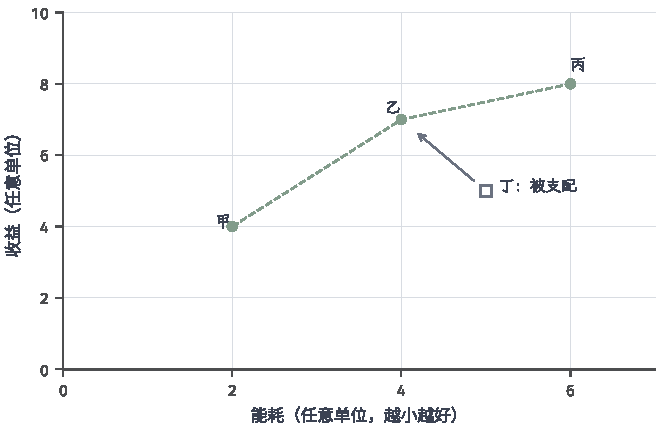
\includegraphics[width=112.000mm]{figures/10-reinforcement-learning/02-information-and-reward/matplotlib/rl-reward-pareto.pdf}
  \caption{收益越大、能耗越小越好。实心点是在四个教学候选策略中的非支配点，空心方块丁被乙支配；虚线只帮助识别候选前沿，不断言连线上的策略全部可实现。}
  \label{fig:rl-reward-pareto}
\end{figure}

据此可以区分几种看似相近的安排。预先给定偏好后求一个策略，与保留多个非支配策略供以后选择，求解的输出不同；多个来源都估计“完好交付”，则仍是同一目标的多份证据。若规定能耗必须低于上限，能耗成为不可任意用收益补偿的约束，而不只是加权分数。约束求解与执行保护由第~\ref{chap:rl-trustworthy}章展开。

% Outline: 5.4.2
\subsection{检测行为与代理奖励的偏差}
\label{sec:rl-reward-detection}

用配送代理给行为打分以前，要先检查代理是否遗漏了已知要求；策略更新以后，还要检查新行为是否超出原反馈覆盖。两种检查都需要在优化前固定独立指标、留出反馈来源和必要情形。例如按路线长度、身份字段完整性与包裹类型分层，可以主动检查训练成功轨迹中少见的情况，只从常见成功轨迹抽样则可能继续漏掉它们。

图~\ref{fig:rl-reward-overoptimization}用解析曲线演示一种待检测现象：代理分数一直上升，按独立标准衡量的行为可能先改善再恶化。两条曲线的差别提醒我们同时查看训练代理和任务证据，不说明所有训练都会遵循这个形状。真实比较还需报告指标口径、采样预算、误差范围与模型选择过程。Gao等研究了奖励模型过度优化的经验现象，本图仍是教学示意，不是该论文的测量结果\scite{gao2022overoptimization}

不同测试可以针对不同缺口。反例测试检查已有怀疑，例如照片看似送达但身份错误；压力测试增加路线长度、载荷或重复次数，考察长时交互及极端路线长度、载荷与重复运行条件。对抗测试主动寻找骗过代理的行为，例如展示别人的签收码；人工审查则分析难以形式化的失败。每次都应记录具体任务条件、行为、分数和验证器版本，使失败可以复查，不能只留下汇总总分。

如果依据留出结果调整奖励或挑选策略，这批证据就参与了开发。下一轮要补充新的独立检查，或明确报告测试复用范围，不能继续把旧结果当作未参与训练、调参与修补的测试记录上的验证。即使没有发现偏差，结论也只适用于已测情形，不能证明所有未见行为均满足要求。

\begin{figure*}[htbp]
  \centering
  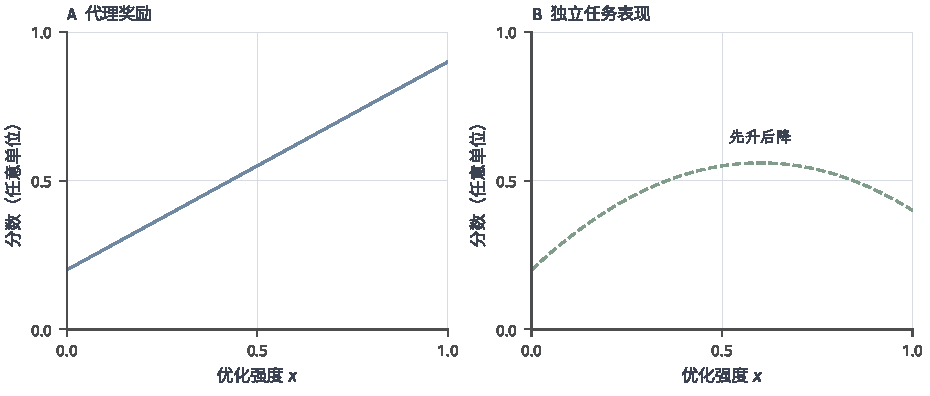
\includegraphics[width=157.400mm]{figures/10-reinforcement-learning/02-information-and-reward/matplotlib/rl-reward-overoptimization.pdf}
  \caption{代理与独立表现可能分离的双面板示意。横轴$x\in[0,1]$是归一化优化强度，曲线分别由$p(x)=0.2+0.7x$与$b(x)=0.2+1.2x-x^2$构造，纵轴为任意单位；不是实验结果，也不表示固定的普遍动力学。}
  \label{fig:rl-reward-overoptimization}
\end{figure*}

% Outline: 5.4.3
\subsection{区分奖励歧义与行为目标偏差}
\label{sec:rl-reward-ambiguity}

两个奖励都解释配送示范时，我们要继续问它们在哪些行为上等价。第~\ref{sec:rl-reward-shaping}节的势差在边界条件满足时保持所有策略的标准期望回报排序，只改变表示；另一些奖励却只在已见示范上相容，在未见路径上作出不同选择。后者限制目标外推，但要认定当前行为失配，仍需比较该行为与独立要求。

\begin{example}[示范相容不等于新路径等价]
  \label{ex:rl-reward-ambiguity}
  假设训练环境只允许专家路径$E$和路径$B$，两个终局奖励都给它们$(2,0)$，于是都支持专家选择$E$。测试环境关闭$E$，另开放此前不可行且未经专家比较的$C,D$。$R_1$给$(C,D)$的分数为$(1,-1)$，$R_2$给$(-1,1)$，而两者仍给$B$记0分。因此，对训练环境中每一条可行路径，两种奖励给出的分数相同；不同路径之间的分数并不相同。测试时两种奖励却分别支持选择$C$和$D$。即使再重复收集一万次训练选择，新增记录仍不涉及$C,D$，不能区分两种目标解释。
\end{example}

在这个例子里，原环境可用的策略可以确定，跨环境重用的奖励却不能确定。恢复原策略、解释专家奖励和恢复可迁移奖励，是强度不同的结论，第三种还要支持新选择的排序。若新状态始终没有反馈，训练得到唯一参数解也可能只是正则化或模型结构替我们作了选择，而不是示范记录识别了唯一答案。

要尝试跨环境重用奖励，一种办法是分开任务计分与依赖原环境转移规律的价值预测。\term{对抗逆强化学习}（adversarial inverse reinforcement learning, AIRL）为此将奖励项和塑形项分别参数化，再用专家与策略转移训练判别器。例如采用
\begin{equation}
  \begin{aligned}
    C(s,a,s')&=\frac{\exp f(s,a,s')}
                         {\exp f(s,a,s')+\pi(a\mid s)},\\
    f(s,a,s')&=g(s,a)+\gamma h(s')-h(s).
  \end{aligned}
  \label{eq:rl-reward-airl}
\end{equation}
其中$g$表示待恢复的奖励项，$h$表示状态上的塑形评分，$f$组合两者；$C$仍取“来自专家”的概率方向。为说明实际更新，令本轮策略$\beta=\pi^{(k)}$，用$\bm\omega$参数化$g,h$，并在式~\eqref{eq:rl-reward-airl}的分母中令$\pi=\beta$，得到$C_{\bm\omega,k}$。专家与本轮策略转移按共同的折扣和吸收协议采样，分别标为1和0。保持$\beta$固定，最大化平衡来源样本的判别对数似然
\[
  \mathcal L_C(\bm\omega)
  =\mathbb E_{\mathrm E}\log C_{\bm\omega,k}(s,a,s')
    +\mathbb E_k\log[1-C_{\bm\omega,k}(s,a,s')] .
\]
两个期望分别对应专家和本轮策略的转移分布；经验更新用各来源批次的平均替代期望，再对$\bm\omega$作梯度上升。两种来源记录的分母都使用本轮$\beta(a\mid s)$，不是在专家记录中换成专家动作概率；在所用状态动作支持上须有$\beta(a\mid s)>0$。

策略更新时冻结学出的$g,h$，原论文采用判别器的对数几率作为奖励，而非直接使用$C$或只使用$f$。由式~\eqref{eq:rl-reward-airl}可得本轮固定的信号
\[
  \widetilde r_k(s,a,s')
  =\log C_{\bm\omega,k}-\log(1-C_{\bm\omega,k})
  =f_{\bm\omega}(s,a,s')-\log\beta(a\mid s).
\]
这一等式说明判别信号包含塑形奖励及温度1的动作熵项；使用该信号时不能再重复加同一熵奖励。用本轮轨迹计算它的回报及优势估计$\widehat A_t$后，可按
$\bm\theta^{(k+1)}=\bm\theta^{(k)}
+\eta\widehat{\mathbb E}_k[
\nabla_{\bm\theta}\log\pi_{\bm\theta}(a_t\mid s_t)\widehat A_t]$
作一次策略梯度更新，梯度在旧参数处计算，$\eta>0$为步长，样本平均按本轮折扣占用加权；多步复用可采用配套的PPO等代理更新。本轮将奖励和优势视为固定，下一轮才刷新策略、转移及判别器分母，不能把冻结$\beta$的代理目标说成任意新策略下的精确熵目标。

三个数值对象可以在一条非终止转移上核算。设$g(s,a)=0.5$、$h(s)=0.2$、$h(s')=0.6$、$\gamma=0.9$，本轮动作概率$\beta(a\mid s)=0.25$。则$f=0.5+0.9(0.6)-0.2=0.84$，判别器专家概率约为$0.903$，实际策略信号为$f-\log\beta=0.84+\log4\approx2.226$。奖励分量、来源概率和训练信号数值不同；迁移讨论需要明确要带走哪个对象，而非统称“恢复奖励”。

迁移时希望重用$g$，而不是整个$f$或上述判别信号。该解释有条件：原论文的恢复分析将一般形式进一步限制为状态奖励$g(s)$，并依赖真实奖励只依赖状态、确定性动态、可分解连通条件、理想最大因果熵专家及优化等假设，且仍有允许的常数歧义。这里的连通条件是：能由同一前驱状态一步到达的两个状态视为相连，再作传递闭包，要求所有状态相连；它使当前状态项与后继状态项能够分离，而不只是要求沿路径可达。一般状态动作奖励、随机动态或有限次优示范，不会仅因写出这个分解就获得无条件恢复保证\scite{rl5-fu2018airl}

这并不意味着所有势差一换环境就失效。若保留依赖实际转移的形式
\[
  R(s,a,s')+\gamma\Phi(s')-\Phi(s),
\]
并用新环境实际后继重新计算势差，满足原边界等条件时仍可相消。若先在旧环境对后继势取期望，保存成固定状态动作奖励
$R(s,a)+\gamma\mathbb E_{T_{\mathrm{old}}}\Phi(s')-\Phi(s)$，
再直接用于新动态，旧转移期望通常不再与新轨迹上的相邻势值相消。AIRL试图区分的正是与旧动态及专家行为纠缠的部分；可否迁移需检查实际奖励形式，不能将失败归于势差本身。

旧动态期望不能直接搬用，可以用两步例子检验。起点势0，中间状态$u$势1、$v$势0，终点势0，$\gamma=0.9$。旧环境动作$A$到$u$，动作$B$到$v$，第二步都到终点；附加回报分别为$0.9+0.9(-1)=0$和0。新环境改为$A$也到$v$，若仍用旧表给$A$第一步加$0.9$，第二步在$v$加0，总和就变成$0.9$，不再与$B$相同。按新实际后继计算势差，两条路径才仍都是0。失效来自保存的旧转移期望，势差的相消形式本身没有改变。

\begin{table*}[htbp]
  \centering\small
  \begin{tabularx}{\linewidth}{@{}>{\raggedright\arraybackslash}p{25mm}*{3}{>{\raggedright\arraybackslash}X}@{}}
    \toprule
    根因 & 可观察症状 & 不能仅凭什么判断 & 补充验证 \\
    \midrule
    代理定义遗漏 & 高分行为违反未编码要求 & 训练集评分准确率 & 要求到证据审计、针对遗漏的反例 \\
    目标反馈不能区分候选奖励 & 多个相容奖励在新行为上分歧 & 奖励参数不唯一 & 有区分力的专家选择或偏好查询 \\
    反馈模型分布外误差 & 新策略行为评分与独立评价不符 & 旧分布拟合误差小 & 新行为重标、覆盖与校准检查 \\
    优化器利用漏洞 & 更新后反复产生某种虚假高分行为 & 单次异常或代理单独上涨 & 固定漏洞复现、版本对照、修补后再测 \\
    \bottomrule
  \end{tabularx}
  \caption{同一种行为偏差可能来自多个根因。奖励歧义本身不等于目标错误，唯一拟合也不能证明标准正确。}
  \label{tab:rl-reward-causes}
\end{table*}

表~\ref{tab:rl-reward-causes}将目标反馈不足、标准遗漏、分布外误差和漏洞利用分开，后两者还可能相互强化。\term{奖励投机}（reward hacking）是策略利用代理缺陷取得高分，却违反原行为要求；\term{过度优化}（overoptimization）是继续加强代理优化时，独立目标可能转而恶化。更新改变行为分布，代理在新区域评分出错，优化又偏向虚假高分行为，就可能形成这种反馈。不过分布外误差未必已被利用，奖励不唯一也未必造成错误行为，仍要用具体反例和独立要求作判断。

% Outline: 5.4.4
\subsection{修订行为目标并约束策略更新}
\label{sec:rl-reward-revision}

发现高分配送有问题后，需要按根因选择修订对象。新增“内部完好”要求，是补充原目标；为同一完好标准补充标签说明，是修订操作性标注规则。重训评分器改进对既定标准的估计，修补允许空字符串通过的验证器则修正实现。四种改动影响不同，必须保留目标、标注、验证器和策略版本，不能统称为奖励模型升级。

修订以后若仍有估计误差，可以惩罚可估计的模型不确定性，用多个奖励模型的分歧定位缺口，或限制策略更新幅度。这些措施各有边界：模型可能共享盲点，不确定性估计也可能失准；保守更新减少进入未见区域的速度，同时可能压低原本可获得的收益。KL约束只控制相对参考策略的偏移，不能补回参考策略已遗漏的要求，平均KL小也不保证每个罕见状态都不变。

新增反例及反馈训练记录应回答已经发现的缺口。例如旧签收照片骗过代理时，可以补充照片与当前包裹身份的一致性检查，再收集不同伪造变体。模型刷新后重测原反例，并检查未参与修补的新变体，才能判断修订是否扩大了正确覆盖。比较时还要记录独立任务指标的变化、采用保守更新后减少的任务收益以及新增反馈成本，不能只报告旧训练集拟合改善。

图~\ref{fig:rl-reward-revision}显示不同修订如何返回检测：目标改动要重新明确要求，估计或实现改动要重新检验新行为。关闭一个反例不表示其他要求都已满足；风险、约束违反和运行时保护还需要第~\ref{chap:rl-trustworthy}章的工具。

\begin{figure*}[htbp]
  \centering
  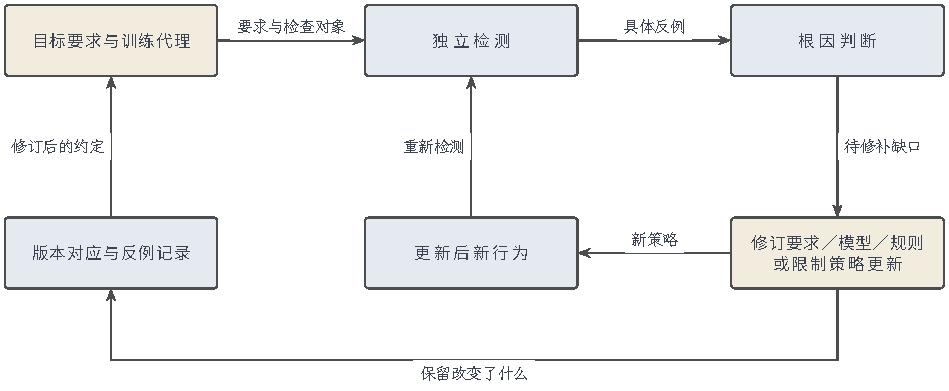
\includegraphics[width=160.616mm]{figures/10-reinforcement-learning/02-information-and-reward/tikz/rl-reward-revision.pdf}
  \caption{目标与代理的诊断回路。检测传递具体反例，根因判断决定改变要求、修订估计还是限制更新；修订后的策略产生新行为，必须重新接受独立检测。}
  \label{fig:rl-reward-revision}
\end{figure*}

% Outline: 5.5
\section{三类奖励限制叠加时的反馈学习}
\label{sec:rl-reward-loop}

真实的配送训练往往同时面临三类限制：只有少量示范、部分路线偏好、若干过程记录，加上一个并不完备的验证器。可以把这些材料组织成一轮可复查的学习闭环：先明确本轮的行为要求与每条反馈的用途，再据此更新有依据的模型或策略，然后用独立证据检验新行为，最后决定是停止还是追加反馈查询。只有在这个闭环里，各步骤才有真实的先后依赖；三类限制本身提供的是不同的诊断依据，并不要求每轮把它们依次消除。如果某种要求始终没有任何反馈涉及，再多次迭代也无法自动解除目标上的歧义。

% Outline: 5.5.1
\subsection{整合已有反馈形成当前反馈约束}
\label{sec:rl-reward-integration}

将配送示范、偏好和检查记录放在一起以前，需要知道它们各自在评价什么。一条可用记录至少包含任务指令与配送条件、被评价行为、反馈值和形式、来源、采样策略及标准版本。轨迹评分还要记录步骤范围和终止原因，偏好还要保留两个候选及呈现顺序。这些字段使我们能够区分冲突来自行为条件、评分尺度还是标准变化。

这里用“反馈约束”概括记录对候选行为和评价模型提供的限制，但实施时必须分开三件事。行为要求规定什么算完成任务，例如交给正确收件人；训练目标规定怎样利用记录拟合模型，例如动作负对数似然和偏好比较损失。策略更新限制则规定本轮允许多大偏移，或排除哪些行为。带噪偏好通常进入损失，不是每条都必须满足的硬不等式；身份要求若作为硬约束，还要有可检查条件和可靠执行机制。

表~\ref{tab:rl-reward-records}按记录、约束对象和本轮用途整合配送反馈。同一批反馈记录可以支持多个模型，但动作标签、相对排序和正确性判断的语义不同，在说明聚合依据前不能直接相加成总分。

\begin{table*}[htbp]
  \centering\small
  \begin{tabularx}{\linewidth}{@{}*{5}{>{\raggedright\arraybackslash}X}@{}}
    \toprule
    反馈记录 & 约束对象 & 可靠范围 & 冲突处理 & 本轮用途 \\
    \midrule
    专家装载动作 & 条件动作分布 & 指令完整的已见状态 & 检查隐含指令与次优示范 & 行为克隆初始化或局部纠正 \\
    同包裹路线偏好 & 相对效用 & 同一偏好群体与标准 & 保留来源分层，不强行平均 & 拟合路线效用差 \\
    装载身份检查 & 步骤关系正确性 & 可读编号且检查器有效 & 与终点身份联合复核 & 提供局部信号 \\
    签收验证 & 最终身份条件 & 签收记录可信 & 排除旧记录与解析漏洞 & 终局反馈；另留独立样本 \\
    少量完好评分 & 包裹状态评价 & 评分尺度一致 & 复核尺度与开箱依据 & 校准反馈模型 \\
    独立开箱审查 & 未覆盖要求的证据 & 被抽查任务范围 & 不用于本轮拟合 & 检查代理遗漏 \\
    \bottomrule
  \end{tabularx}
  \caption{同一轮反馈记录的五项对应。独立证据应按样本和用途隔离，不能一边参与拟合一边称为留出检验。}
  \label{tab:rl-reward-records}
\end{table*}

假设专家走楼梯，偏好却选择电梯。先比较包裹是否易碎、当时电梯是否可用、评价者是否强调节能；只有条件和标准相同时，才需要进一步判断来源可靠性或专家是否次优。装载检查通过而终局身份失败，也可能来自中途换包，局部标签各自都正确，但跨步骤一致性被破坏。保留条件和粒度才能定位这些差异，平均正负分反而可能掩盖原因。

整合后，本轮要确定明确的要求、训练目标和更新限制。例如先要求身份正确，再在满足身份条件的行为中比较完好与能耗；用动作示范拟合策略，用路线偏好和完好评分分别拟合比较模型及评分模型。策略更新还可以采用参考KL惩罚或约束，但必须说明是哪一种。身份优先的文字约定并没有自动提供动作过滤器，硬性执行能力仍要验证。所有约定都应附上适用任务条件与可得观测范围及尚未解决的分歧。

若分歧确实来自不能兼容的真实偏好，可以保留按偏好条件选择的策略或多个候选。必须聚合时，应解释分数单位、尺度、权重及权重代表的取舍；加权平均是一个新约定，不是争议已经被识别为唯一真实目标的证据。

% Outline: 5.5.2
\subsection{依据反馈约束联合更新模型与策略}
\label{sec:rl-reward-joint-update}

已有反馈及其用途确定后，要明确本轮改动哪些学习对象。对应记录可用于拟合奖励、效用或通过概率模型，归因机制再把轨迹结果转成局部信号，策略在本轮惩罚或约束下利用这些信号更新，并产生下一批行为。价值基线帮助降低方差或自举，不替代已经约定的行为评价标准。“联合更新”可以是交替拟合，也可以只改其中一项，不要求全部参数同时反向传播。图~\ref{fig:rl-reward-update}标明反馈记录、归因结果与参数更新之间的依赖，以及本轮冻结的标准和参考策略。

\begin{figure*}[htbp]
  \centering
  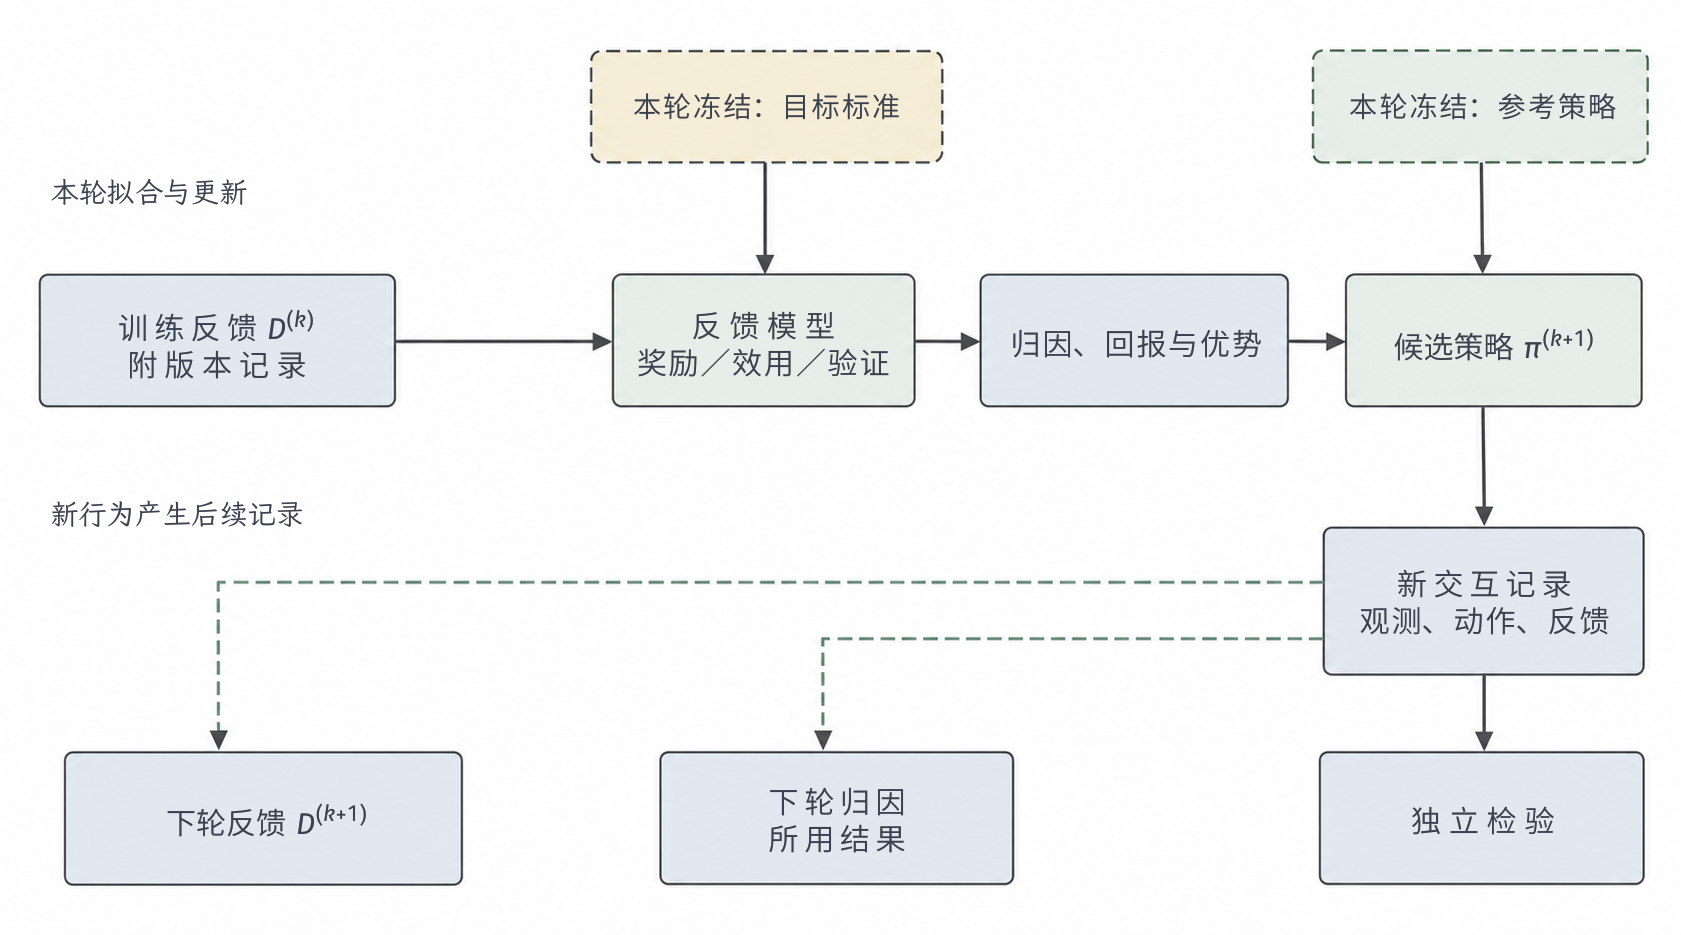
\includegraphics[width=157.400mm]{figures/10-reinforcement-learning/02-information-and-reward/generated/rl-reward-update/figure.png}
  \caption{本轮更新及下一轮补充的记录依赖。实线表示从本轮训练反馈形成反馈模型、局部信号和候选策略的依赖；候选策略产生的新交互记录，沿虚线回流箭头进入下一轮的反馈整合或归因。虚线框表示本轮冻结的目标标准和参考策略。独立检验记录不回流本轮拟合。}
  \label{fig:rl-reward-update}
\end{figure*}

在这条更新路径中，反馈来源和优化器是两个选择。RLHF与RLAIF可以采用相同策略优化器而使用不同评价者；迭代式偏好优化可以每轮补新偏好，再运行DPO；在线RLVR则对当前策略样本即时调用规则验证。\term{解耦剪裁与动态采样策略优化}（Decoupled Clip and Dynamic sAmpling Policy Optimization, DAPO）是其中一种具体更新方法。表~\ref{tab:rl-reward-loops}比较各轮更新和固定的对象，以及样本和反馈何时刷新，而不是将这些名称当成互斥算法类别。

\begin{table*}[htbp]
  \centering\small
  \begin{tabularx}{\linewidth}{@{}>{\raggedright\arraybackslash}p{23mm}*{3}{>{\raggedright\arraybackslash}X}@{}}
    \toprule
    路线 & 本轮更新对象 & 本轮固定对象 & 采样与反馈刷新 \\
    \midrule
    PPO式RLHF & 奖励模型、策略及价值可分阶段更新 & 标注标准、参考策略；策略阶段冻结奖励 & 当前策略采样，按预算补人类偏好 \\
    RLAIF & 反馈模型与策略，依实现可有价值模型 & AI评价模型、提示与标准的指定版本 & 新样本交由AI评价，独立抽查 \\
    迭代式偏好优化 & 偏好对上的策略参数 & 单轮偏好集与参考策略 & 外层采样和标注刷新，内层可离线DPO \\
    在线RLVR & 策略；基线依更新器而定 & 验证规则、参考答案或程序测试用例 & 新策略候选逐批验证 \\
    DAPO & 无独立评论家的策略更新 & 当前验证规则、旧策略批次概率 & 动态采样补充混合得分组，按token聚合损失 \\
    \bottomrule
  \end{tabularx}
  \caption{反馈闭环而非互斥算法分类。DAPO是在线可验证反馈的一种具体实现，RLAIF也可以组合不同的策略优化器。}
  \label{tab:rl-reward-loops}
\end{table*}

表中的DAPO修改集中在剪裁、样本筛选和损失聚合。它在所讨论训练设置中使用规则结果奖励，去掉参考KL项，采用不同的上下剪裁阈值，并动态补充组内同时产生成功和失败回答的任务提示。损失还从式~\eqref{eq:rl-reward-grpo}的回答内平均，改为对全部有效token平均。为比较长度权重，记剪裁项为$\ell_{i,t}$，两种聚合是
\begin{equation}
  \frac1m\sum_i\frac1{T_i}\sum_t\ell_{i,t},
  \qquad
  \frac1{\sum_iT_i}\sum_i\sum_t\ell_{i,t}.
  \label{eq:rl-reward-dapo-weight}
\end{equation}
前者赋予每个回答相同总权重，后者赋予每个token相同权重，使长回答在整批损失中占更大总权重。超长惩罚与截断处理也会改变反馈语义；论文称之为reward shaping，不意味着满足本章的潜势型不变条件。DAPO发表于NeurIPS 2025，但经验结果只对应报告中的模型、数学任务和预算，不能推出这些组件对所有任务都有收益\scite{rl5-yu2025dapo}

长度聚合的差别可以在两个回答上直接算出。令长度为2和4，各token剪裁项分别为1和$-1$。先各回答平均再平均，值为$(1-1)/2=0$；对全部token平均则为$(2-4)/6=-1/3$。前者让两回答总权重相同，后者让较长的负项回答占更多权重。两个代理数值只是权重差的示例，不表示真实任务回报也发生了同样幅度的变化。

动态采样补混合得分组，可以减少零相对信号，但筛选也改变被选入训练的任务提示分布，被丢弃候选仍消耗采样和验证预算。过滤整组失败的困难题，没有解决这些题。提高剪裁上界只是改变代理目标梯度何时饱和，不是对动作概率施加硬上限。因而比较实现时，应同时记录样本选择、组内标准差分母、长度聚合方式和验证器版本。

\begin{example}[一轮可复查的更新记录]
  \label{ex:rl-reward-round}
  假设教学轮次$k=3$使用训练反馈记录$D^{(3)}$、身份与完好标准$\texttt{std-2}$、反馈模型$\texttt{feedback-3}$、旧策略$\pi^{(3)}$和参考策略$\pi_{\mathrm{ref}}$。$D^{(3)}$有20条装载动作、12对偏好、8条完好评分，分别用于策略拟合、比较模型拟合和评分模型拟合，后两项组成$\texttt{feedback-3}$。策略更新时冻结$\texttt{std-2},\texttt{feedback-3},\pi_{\mathrm{ref}}$，独立审查记录不加入$D^{(3)}$。

  再取两条等长四步轨迹，以本轮约定的综合代理$\widetilde R$给终局记1和0分，中间奖励为零，$\gamma=0.9$，于是起点回报为$0.729$和0。冻结基线为$0.3645$，减去基线得到样本优势$0.3645$和$-0.3645$。只更新起点二动作的logit，其他动作规则固定；初始logit为0，两条轨迹各来自一个起点动作，样本平均梯度为$0.18225$。令步长为$0.2$、KL系数为$0.1$，且当前策略恰与参考相同，精确KL梯度此时为零。一次未剪裁更新得到logit $0.03645$，正优势动作概率约为$0.5091$，作为候选$\pi^{(4)}$。

  本轮记录目标为“轨迹代理回报的PPO式改进减参考KL”，并分别预留40个访问状态动作标签、20对比较、100次验证和10次人工审查的预算上限。更新后要分开检验$\texttt{feedback-3}$是否更符合反馈和$\pi^{(4)}$是否改善实际行为。这些计算是可复查的教学记录，不是实际测得的任务回报。
\end{example}

% Outline: 5.5.3
\subsection{用更新后行为检验反馈约束的有效性}
\label{sec:rl-reward-loop-check}

候选$\pi^{(4)}$产生新行为后，要按本轮开始前的标准检查，不能只重算$\pi^{(3)}$的旧日志分数。三类限制分别对应三个问题：新状态是否超出反馈覆盖，局部信号是否仍正确联系关键动作与结果，代理回报增加时独立行为指标是否改善。表~\ref{tab:rl-reward-checks}分列相应证据和失效判据，使一种检查通过不能替代其他检查。

\begin{table*}[htbp]
  \centering\small
  \begin{tabularx}{\linewidth}{@{}>{\raggedright\arraybackslash}p{20mm}*{4}{>{\raggedright\arraybackslash}X}@{}}
    \toprule
    检查 & 待检查行为与任务条件 & 独立证据 & 失效判据 & 仍未覆盖范围 \\
    \midrule
    观测与覆盖 & 新策略访问状态、长短轨迹 & 新状态专家标签、留出来源评分 & 无支持区域仍被赋予高置信评价 & 未覆盖的任务条件和状态动作 \\
    局部归因 & 关键步骤与相关标记 & 受控扰动、过程复核、终局结果 & 无关标记改变信号，关键错误不受罚 & 不可干预步骤的因果贡献 \\
    目标匹配 & 代理高分的新行为 & 独立身份、完好和成本检查 & 违反已约定要求或独立指标退化 & 未形式化与难观测要求 \\
    来源一致性 & 同行为的多来源判断 & 第三方执行或事实核对 & 分歧无法由条件差异解释 & 一致来源的共同盲点 \\
    \bottomrule
  \end{tabularx}
  \caption{检验必须说明未覆盖范围。来源一致性可以暴露冲突，却不能替代外部事实证据。}
  \label{tab:rl-reward-checks}
\end{table*}

检验结果应区分证据支持、证据不足和明确失效。若$\pi^{(4)}$在预定短路线、身份可读范围内完成全部检查，估计精度也达到事先要求，可以支持当前反馈在这个范围有效。若只测三次且均成功，仍未覆盖必要长路线或满足精度要求，就只能说暂未发现失败。若已有代理高分却交错收件人的行为，便得到明确反例；平均成功率高不能抹去这个失效。

暂未看见失败也可能只是样本少。假设固定策略在同一测试条件下每次独立有$0.1$错误率，三次都通过的概率仍为$0.9^3=0.729$。因此“三次通过”在这样的策略下很常见，不能单独证明错误率很低。这个概率不是看到三次通过后的错误率后验；它说明接受结论还需事先约定的统计精度和覆盖依据。

诊断要返回对应缺口：新状态无标签就补访问覆盖，关键步骤局部信号错误就修订归因，完好要求未编码就修订标准或代理。这样可以针对已有证据改变相关对象，不必一次失败就重训全部模型。反例若进入下一轮修订，就成为开发记录，后续不能再将它单独称为独立留出检验。

% Outline: 5.5.4
\subsection{依据检验结果与反馈预算决定停止或继续}
\label{sec:rl-reward-stopping}

即使新行为全部通过已做检查，也需要判断检查是否达到了事先约定的要求。训练前应固定独立指标的接受标准、必要覆盖、统计精度或不确定性要求，以及各类预算上限，不能看到结果后再放宽门槛。有限测试可以支持限定范围的接受，不为未测范围提供“没有失败”的保证。

\begin{table*}[htbp]
  \centering\small
  \begin{tabularx}{\linewidth}{@{}>{\raggedright\arraybackslash}p{23mm}*{3}{>{\raggedright\arraybackslash}X}@{}}
    \toprule
    证据状态 & 允许的后续动作 & 必须保留的结论范围 & 所需反馈或检查记录 \\
    \midrule
    达到预设充分性与接受标准 & 停止训练，保留复核入口 & 只接受已测任务、标准和策略版本 & 已完成覆盖、精度及成本记录 \\
    未发现失败但证据不足 & 有预算则定向查询；否则停止或收窄范围 & 未证实原范围满足要求；预算停止不等于成功 & 缺少的场景、样本或独立来源 \\
    已发现明确失效 & 暂停对该范围的接受，修订后再测；或终止 & 记录反例与不适用范围 & 根因、修补方案、验证与查询成本 \\
    \bottomrule
  \end{tabularx}
  \caption{停止训练是一种行动，接受行为是一个证据结论，二者不能混同。}
  \label{tab:rl-reward-stopping}
\end{table*}

表~\ref{tab:rl-reward-stopping}区分停止行动和接受结论。满足预设要求可以停止，预算耗尽也可以停止，但后者仍可能留有关键缺口。若获准查询只能看终点照片，不能观察包裹内部，重复评价也无法识别完好要求；这时应收窄结论或改变反馈可读取的字段或查询权限，而不是将次数当作充分性。

有剩余预算时，还要说明下一批反馈可能改善哪项判断：当前状态覆盖、候选目标排序、过程贡献或验证规则。可以估计查询减少多少候选模型分歧、是否可能改变决策，再与人工时间、采样和执行成本比较；没有用于校准查询收益估计的已有记录时，这些只是启发式依据，不是有数值保证的查询后决策收益。更换目标、反馈标准或明显改变策略访问分布后，原停止证据所对应的对象也变了，需要重新检查。

\begin{algorithm}[反馈学习的继续与停止闭环]
  \label{alg:rl-reward-loop}
  \begin{algorithmic}[1]
    \Require 目标标准、独立接受条件、必要覆盖、分项预算、初始反馈与策略
    \Ensure 候选策略、结论范围、停止原因和未解决缺口
    \While{尚未记录停止原因}
      \State 整合兼容的反馈，固定本轮标准、本轮训练反馈记录的范围及未解决分歧
      \State 只更新有相应证据支持的反馈模型、归因机制或策略
      \State 以新行为接受独立检查，分类为充分、证据不足或明确失效
      \If{覆盖与精度充分，且满足预设接受条件}
        \State 记录“在已检验范围满足要求”，停止本轮学习
      \ElsIf{预算不足，或允许查询不能区分关键目标解释}
        \State 记录“预算停止”或“识别受限”，收窄结论并停止
      \Else
        \State 按观测、归因或目标缺口选查询，必要时先修订目标标准
        \State 获取新反馈，记录成本、生成策略与标准版本，返回整合
      \EndIf
    \EndWhile
  \end{algorithmic}
\end{algorithm}

算法~\ref{alg:rl-reward-loop}只更新有相应证据支持的对象，不要求每轮全部模型变化。明确失效可能先需要修订要求，而不是马上增加样本；若获准查询无法补足缺口，也可以停止优化错误代理，并保留未解决结论。这个规则控制反馈学习是否继续，不替代系统部署审批或运行流程。

% Outline: 5.5.5
\subsection{针对反馈缺口获取新反馈}
\label{sec:rl-reward-query}

决定继续后，还需把未决问题转成可执行查询。例如错误走廊缺恢复动作，就查询该状态上的专家标签；两条新路线排序不定，就比较候选奖励意见不同的路线。表~\ref{tab:rl-reward-queries}按这类缺口列出查询能排除的解释，同时保留查询之后仍未回答的部分。

\begin{table*}[htbp]
  \centering\small
  \begin{tabularx}{\linewidth}{@{}*{4}{>{\raggedright\arraybackslash}X}@{}}
    \toprule
    具体缺口 & 查询方式 & 可以排除的解释 & 仍不能回答什么 \\
    \midrule
    偏离后不会恢复 & 当前访问状态上的专家动作 & 这些状态上的错误动作候选 & 唯一真实奖励与未查询状态 \\
    新路径排序不确定 & 比较奖励候选意见不同的路径 & 对该比较给出相反排序的目标 & 其他任务条件或评价群体的偏好 \\
    关键过程贡献不清 & 步骤标注、受控检查与结果对照 & 局部无效却被奖励的归因 & 未控制混杂下的完整因果结构 \\
    验证标准遗漏 & 新结果检查、规则边界与对抗案例 & 会接受已知错误行为的验证器 & 未被形式化的全部要求 \\
    来源共同偏差 & 独立来源和实际执行审查 & 仅依赖共同代理的解释 & 未审查行为的真实性 \\
    \bottomrule
  \end{tabularx}
  \caption{查询应取得能区分候选奖励或反馈模型的评价结果，而不只是重复已经一致的反馈。}
  \label{tab:rl-reward-queries}
\end{table*}

可回接前面的新路径歧义：两个奖励都给训练路径$E,B$相同分数，再比较这两条路径不会区分它们；两奖励对$C,D$却给相反排序。针对$C,D$取得同条件、同评价标准的比较，才可能提供新的区分证据。若反馈有噪声，还需控制误排序，而不能把一次回答当作排除所有其他解释。查询的价值在于回答未决问题，不在于再增加一条已经一致的标签。

查询的选择依据也不同。DAgger查询当前访问状态的专家动作，主动偏好查询选择可能改变候选排序的比较；不确定性采样选择反馈模型分歧大的行为，在线验证检查当前策略产物，对抗收集则寻找代理漏洞。但模型分歧的大小未必反映新反馈对真实行为要求的区分程度：共同盲点可能让模型一致自信，模糊措辞却可能造成很大分歧而不改变行为要求。保留独立随机或分层抽查，可以检查主动筛选是否遗漏重要区域。

沿示例~\ref{ex:rl-reward-round}，假设$\pi^{(4)}$主要缺恢复动作，可以查询6个实际访问状态的动作；为新路线再补4对偏好、24次验证和2次人工审查。还要分别记录取得候选所用轨迹数及环境步数。这些教学计数单位不同，相加成“36条反馈”不能说明成本；每批记录应附带生成策略$\pi^{(4)}$、标准$\texttt{std-2}$及采样筛选协议。

新反馈返回第~\ref{sec:rl-reward-integration}节时，先核对与旧标准的兼容性。沿用$\texttt{std-2}$的记录可聚合；若$\texttt{std-3}$新增内部破损要求，旧终点照片标签只支持原先被检查的条件，需视用途重标或分开使用，不能直接当作$\texttt{std-3}$的完整正例。若全部获准查询只比较速度，就仍无法区分看重完好和看重能耗的目标解释。此时应报告识别边界，闭环轮数没有补足区分这些目标解释所需的评价记录。

% Outline: 5.6
\section{本章小结}
\label{sec:rl-reward-summary}

回到配送中的反馈缺口，替代记录首先决定我们能学到什么。示范约束动作或长期占用，评分和偏好约束评价函数，验证只判断明示条件；它们不相互等价，也不必都先还原为唯一奖励。BC在已有专家分布上拟合，DAgger补当前访问状态；奖励模型加策略优化需要评分新行为，标准DPO拟合固定偏好对。GRPO怎样比较组内候选，则与分数是否来自规则是两个选择。

取得结果以后，还要判断它怎样支持早期动作更新。结果回溯重新记账，过程监督增加证据，奖励变换和辅助目标改变信号或训练位置，各有成本与保持条件。潜势塑形在有界势、共同初始分布及正确终端处理下，靠相邻势项相消保持标准期望回报排序；这不证明局部信号具有因果意义，也不保证风险排序或学习速度不变。

最后，训练信号是否表达行为要求，要用独立证据检验。反馈拟合准确不证明标准完整，相容奖励也可能在未比较行为上分歧；它们若一致支持当前策略，结论也应保留相应范围。每轮反馈学习都要固定标准、更新对象和检验证据，再取得能补具体缺口的新反馈。停止时说明是已在限定范围满足要求、预算耗尽，还是允许的查询仍无法识别关键目标。


\bookpart{任务扩展与可信决策}{Task Extensions and Trustworthy Decisions}
\label{part:rl-task-expansion-and-trustworthiness}

\BookPartGuide{%
一个策略在固定任务中取得较高回报，还不足以说明它能迁移到新任务、与其他行动者协作，或在安全约束下执行。任务改变会影响已有交互记录的适用范围，其他行动者的选择会改变行为后果，风险与安全要求则会改变策略的比较标准。本部分沿这三种扩展，检查可以复用什么、怎样训练与适应，以及哪些证据足以支持执行。

第~\ref{chap:rl-transfer}章“任务泛化与适应”先确定可复用的是表示、策略、价值、模型还是学习规则，再说明这些对象适用于哪些任务。训练任务与评价任务的划分、允许取得的目标任务交互记录、适应预算和参数更新权限共同界定问题；在这些条件下，才能比较直接迁移、基于历史的适应与基于梯度的适应，并诊断迁移退化的原因。

第~\ref{chap:rl-multi-agent}章“多智能体协作和博弈”把单一行动者扩展为多个相互影响的参与者。收益关系决定协作、竞争或混合的行为标准；各自能够读取的观测、历史与消息决定可执行策略。联合交互记录的收集、价值估计与策略更新需要共同处理其他参与者的依赖和变化，集中训练时可取得的状态也不能自动供分散执行使用。

第~\ref{chap:rl-trustworthy}章“可信强化学习”把期望回报之外的风险、模型偏差、安全约束与可靠性要求写成可检验主张。风险敏感目标、鲁棒优化、受约束学习和执行时保护分别改变不同环节，所提供的保证依赖各自的模型、扰动集合、评价协议或安全证书。三章最终都要回到适用任务、比较预算与失效条件：一次测试成功只能支持对应范围的主张，条件改变后需要重新评价。}


% Outline: 6
\chapter{任务泛化与适应}
\label{chap:rl-transfer}

前几章始终在“同一个任务”里学习：地图、终点、移动规律和奖励一旦定下，训练和部署面对的都是它。但现实中的任务很少一成不变。设想一辆小车已经学会绕过障碍：若终点换到地图另一侧，它仍然知道各方向怎样移动，只需重新选择路线；若地图不变而地面变滑，原来那条路线的到达概率就可能改变。两种变化都在问“旧知识能不能用于新任务”，可需要保留的东西和需要重新估计的东西截然不同。这就是本章的主题——任务泛化与适应：把在一批任务上学到的知识，用到没见过或已经变化的新任务上。除了“什么变了”，还有两个同样关键的问题：小车是否被告知新终点或地面参数？是否允许它通过试探弄清这些？共享的物理规律、取得的目标描述或任务交互记录、以及获准学习的权限，是三个互不替代的条件。

第~\ref{chap:rl-learning}~章已经说明怎样在单个任务中学习价值、策略与环境模型。现在把这些学习对象放到多个任务之间考察：声明哪些要素允许变化后，才能判断某个预测或行为规则是否仍有原来的含义；声明可读取的任务描述、观测和交互预算后，才能确定新任务中的策略如何形成。训练负责获得可复用知识，部署负责调用或调整这些知识，验证则检查所声明的任务范围内是否确有收益。图~\ref{fig:rl-transfer-map}~中的反馈箭头表示，失败有时要求重查共享假设，而不只是延长训练。历史能否保留会影响动作选择的观测、动作与奖励记录、固定日志能否支持新行为，分别沿用第~\ref{chap:rl-information}~章的信念与覆盖条件；反馈究竟评价什么，仍由第~\ref{chap:rl-reward}~章的目标规定。

\begin{figure*}[t]
  \centering
  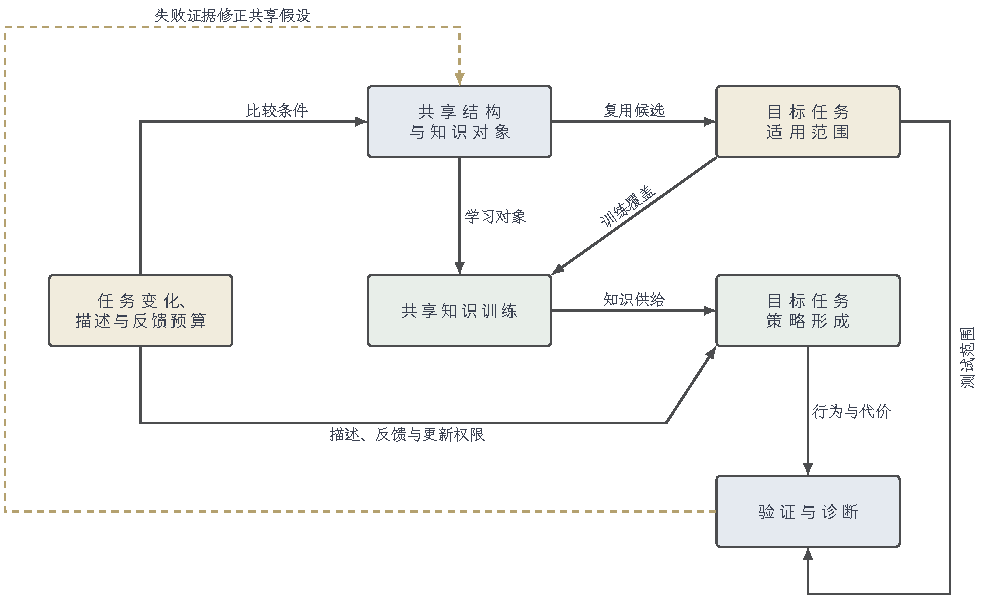
\includegraphics[width=166.345mm]{figures/10-reinforcement-learning/03-task-expansion-and-trustworthiness/tikz/rl-transfer-map.pdf}
  \caption{任务泛化与适应的论证关系。实线标明条件约束或知识供给，虚线表示验证后的修订反馈；不是所有方法都必须顺序执行的流程。部署中的记忆、参数更新和持续交互可以组合。图为本章关系的原创示意。}
  \label{fig:rl-transfer-map}
\end{figure*}

% Outline: 6.1
\section{任务泛化与适应问题}
\label{sec:rl-transfer-problem}

% Outline: 6.1.1
\subsection{任务要素的变化范围}
\label{sec:rl-transfer-components}

沿用前文宽4、高3、障碍位于$(2,2)$的导航地图，起点仍为$(1,1)$。基准任务以$(4,3)$为终点，合法意图方向以$0.8$概率执行，两侧各以$0.1$概率滑移；进入终点得1，其他非终止步得$-0.04$，吸收后奖励为0，折扣为$\gamma=0.9$。这些是统一的教学设定，不是实验测量结果。我们分别改变终点、移动噪声、观测符号或动作编码，观察旧策略会在哪一步失去依据：终点决定去哪里，移动规律决定动作会到哪里，观测符号决定怎样解释当前收到的观测，动作编码决定命令的物理含义。为把这些变化放在同一套记号下比较，用$c$标识一项任务，并把所有允许的任务组成任务族。

\begin{definition}[任务族]
  \label{def:rl-transfer-family}
  给定非空任务参数集合$\mathcal C$和共同折扣$0\leq\gamma<1$。对每个$c\in\mathcal C$，状态空间$S_c$、行动空间$\mathsf A_c$和观测空间$\mathsf O_c$均配可测结构，每个状态有非空合法动作集$\mathsf A_c(s)$。初态分布$\mu_{0,c}$是$S_c$上的概率测度，$T_c$是从合法状态—动作对到$S_c$上概率测度的转移核，$K_{o,c}$是按声明时序产生观测的概率核，$R_c(s,a)$是可积逐步奖励在状态动作给定后的条件均值。
  用$c$索引任务模型
  \[
    \mathcal M_c=(S_c,\mathsf A_c,T_c,R_c,K_{o,c},\mu_{0,c},\gamma).
  \]
  其中动态环境部分记为$\mathcal E_c=(S_c,\Sigma_{S_c},\mathsf A_c,\Sigma_{A_c},\mu_{0,c},T_c)$。任务族由动态环境、奖励与终止反馈机制、观测机制，以及执行前提供的任务描述和可记录字段共同确定。比较时须声明哪些分量随$c$改变，哪些共同固定；有终止事件或有限时域时，还须规定终止机制与时域。
\end{definition}

同一状态集合上的两个奖励函数已经定义了不同任务；状态和动作的维数相同，并不要求转移、奖励或语义相同。若要根据随机奖励和终止反馈辨识任务，还须给出这些反馈与后继状态的联合条件分布：均值$R_c$本身不能确定反馈似然。表~\ref{tab:rl-transfer-changes}~列出四种单因素变体，其中执行前可读的描述或参数由实验协议提供，不是把智能体训练中读取过的任务标签或参数一概当作已知。

\begin{table*}[t]
  \centering\small
  \begin{tabularx}{\linewidth}{@{}>{\raggedright\arraybackslash}p{23mm}*{3}{>{\raggedright\arraybackslash}X}@{}}
    \toprule
    变化分量 & 保持不变的对象 & 执行前可读的描述或参数 & 需要重算或重新学习的对象\\
    \midrule
    终点与奖励 & 地图、物理移动规律 & 可能提供目标坐标；也可能只有到达反馈 & 新目标价值、路线选择；终止规则改变时还包括有效转移\\
    移动噪声 & 目标含义、地图、命令语义 & 位置与移动结果；风参数未必给出 & 转移概率、长期后果、控制策略\\
    观测符号 & 潜在地图与物理动作 & 新符号图像；对应表可能未知 & 感知对齐，必要时重学历史表示\\
    左右命令互换 & 物理空间、目标、观测 & 命令标签与执行结果 & 动作映射、合法命令集与技能接口\\
    \bottomrule
  \end{tabularx}
  \caption{同一导航地图中的任务变化。每行单独改变一个因素，数字与任务均为教学构造。更换吸收终点会改变完整MDP的转移核，不能只因物理移动规则相同就声称共同动力学。}
  \label{tab:rl-transfer-changes}
\end{table*}

表中的终点变化还需要检查吸收约定。如果进入终点后不能继续移动，换终点就同时改变了转移核，不能只归为奖励变化。要单独检验奖励能否复用，我们改用共同终止规则：所有任务在相同时间结束，或保持固定吸收出口而只改变沿途地标的奖励。有限时域的前一种设定还须把剩余时间纳入状态，才能用同一个转移核描述到时终止。这些独立变体用于隔离复用条件，不是基准网格的另一组求解结果。

还要区分两个时间尺度。在一次适应试验中，未知风向可以固定不变，只是智能体逐渐认识它；也可以每个回合都改变。前者的证据指向同一估计对象，后者的旧证据可能已经过时。固定任务辨识在第~\ref{sec:rl-transfer-identification}~节展开，变化任务的跟踪在第~\ref{sec:rl-transfer-tracking}~节另行定义。

% Outline: 6.1.2
\subsection{目标任务信息的可用条件}
\label{sec:rl-transfer-information}

同样是换终点，地图直接标出坐标时，小车可以据此规划；只有抵达才发奖励时，它需要从经历中排除候选位置。若隐藏的是风向，即使终点已知，也可能要试一次移动才能区分转移规律。前一小节比较任务中什么发生了变化，这里固定这些变化，转而检查智能体能看见什么。已知目标只能消除目标身份的不确定性，不能同时消除动力学的不确定性。

执行前提供的目标坐标、参数或语言指令称为\term{显式任务描述}（explicit task description）：它直接告诉智能体任务的某些条件。描述未给出的条件，可以从已记录的观测、动作、奖励与终止标记中推断，下文将这组按时间保存的记录称为\term{任务交互记录}（task interaction records）。若现有记录不足以区分候选任务，还可以选择会产生不同反馈的动作；这种\term{主动辨识}（active identification）通过行动取得能区分候选任务的新观测或奖励，不是对同一份历史多计算几遍。语言指令也需要与奖励和控制接口有可信的对应关系，单独一句话并没有给出完整MDP。

设训练任务用编号1和2分别代表东、西两个终点。把编号交换、保留所有轨迹的物理内容，再相应交换训练标签，并不会改变问题难度。对于从未出现的编号3，训练记录没有告诉模型它是北端终点还是强风任务。编号能索引记住的任务，却没有坐标那样的几何语义。新编号上的零样本迁移必须另有描述映射，不能依靠编号的大小顺序。

任务编号不自带物理含义，历史编码器的输出$\bm z_t$也不自带概率含义。奖励预测或策略损失可以使这个向量保留与任务有关的线索，但没有保证它的分量构成归一化、校准的任务后验。还要先检查历史本身是否有区分力：若两个任务在所有获准动作下都产生相同的可见反馈分布，增加历史长度或模型容量也无法区分它们。第~\ref{sec:rl-transfer-belief}~节据此分别考察记录本身不能区分任务和推断器未利用已有区分线索的情形。

% Outline: 6.1.3
\subsection{零样本、少样本与持续适应预算}
\label{sec:rl-transfer-budget}

一个网络保持权重不变，却可能在历史窗口中读过大量目标任务反馈；另一个网络在固定日志上更新参数，却没有增加真实交互的权限。只报告是否更新网络，无法判断两者各用了多少目标任务观测、奖励与终止反馈。比较预算时，需要同时记录可读取的任务描述、观测及交互记录，会变化的记忆或参数，以及推断和更新所需的计算。

本章将\term{零样本执行}（zero-shot execution）限定为不使用目标任务反馈进行额外学习、记忆适应或模型选择的执行。它仍可读取给定任务描述和正常控制所需的观测。部分可观测任务中的状态滤波应预先声明：在已给定任务模型下估计当前位置，属于控制所需的状态估计；利用偏移反馈推断未知风向，则更新了对未知任务参数的判断，属于适应，即使只发生在一个回合内、网络权重始终不变。\term{少样本适应}（few-shot adaptation）使用预定数量的目标经验形成策略；经验可以来自给定日志，也可以来自获准交互。\term{持续适应}（continual adaptation）允许在部署过程中反复更新任务参数估计、潜变量记忆或策略，评价必须计入这一过程中的表现。

文献中的zero-shot可能采用不同口径，例如仅要求测试时不更新网络权重。比较论文结果时，应继续核对实际读取了哪些目标任务反馈、是否保留任务特定记忆、是否据此选择模型，再按本章预算分类；论文名称本身不能代替这些协议。

表~\ref{tab:rl-transfer-budget}~用教学协议固定这些差别。$B$表示适应交互步数，$L$表示最多保留的历史长度，$K$表示梯度步数；实际论文还应报告各回合长度，不能仅以“若干回合”比较不同任务。

\begin{table*}[t]
  \centering\small
  \begin{tabularx}{\linewidth}{@{}>{\raggedright\arraybackslash}p{19mm}*{6}{>{\raggedright\arraybackslash}X}@{}}
    \toprule
    协议 & 目标交互 & 可见反馈 & 上下文 & 参数更新 & 额外计算 & 选模查询\\
    \midrule
    零样本 & 无适应步；执行另计 & 描述、执行观测 & 不累计用于辨识未知任务的反馈 & 0 & 固定推理预算 & 0\\
    固定日志适应 & 新交互0 & 日志给定字段 & 至多$L$步 & 至多$K$步 & 推断与反传均计 & 预先固定\\
    少量在线适应 & 总计$B$步 & 约定奖励及终止 & 至多$L$步 & 至多$K$步 & 探测、规划均计 & 纳入$B$\\
    持续在线适应 & 全程累计 & 按到达时刻可见 & 记忆重置规则固定 & 频率与总量均报 & 每步和累计成本 & 不用未来成绩选模\\
    \bottomrule
  \end{tabularx}
  \caption{目标任务预算的不同分量。各列共同定义协议；“固定日志”与“固定参数”不是同义词。本表为评价口径，不是任何算法的实测回报。}
  \label{tab:rl-transfer-budget}
\end{table*}

假设每回合恰有20步，共运行10回合，这是教学预算而非实测配置。只报告第1回合、按固定控制规则响应观测且不辨识任务或更新策略，回答的是初始执行能力；允许在10回合内学习并报告全部200步回报，回答的是学习期间能否付得起试错成本；先适应10回合，再停止任务学习、另测5回合，回答的是200步适应后的控制能力，但总交互已是300步。三种分数即使相等，也没有相同含义。

初始执行只按预定规则控制和恢复，不包含用于学习任务的探测或选模；允许适应的两种评价，则还要计入这些操作的成本。试探风向和从失败位置返回消耗交互步，选择“最好的第7次更新”则需要查询目标任务成绩。只有把协议允许的这些成本计入，才能比较相同反馈量或计算上限下谁较早达到预先规定的回报，而不是只比较最终执行了多少步。

% Outline: 6.2
\section{可复用决策知识的确定}
\label{sec:rl-transfer-knowledge}

% Outline: 6.2.1
\subsection{由任务要素异同判断共享结构}
\label{sec:rl-transfer-sharing}

有了任务变化、可读取的描述与交互记录、适应预算这三个比较依据，现在可以回到核心问题：哪些旧知识在新任务里仍然“有意义”？看两个对比鲜明的例子。在共同终止规则下只换导航目标，旧的转移模型仍能正确预测“向右会到哪里”；可一旦把左右命令互换，原策略发出的“右”却会执行成向左。两种新任务的观测编码与动作命令都可以沿用相同的张量形状，但只有前者保留了原命令的控制含义。可见“接口长得一样”并不代表“含义一样”。图~\ref{fig:rl-transfer-components}~逐项标出哪些任务分量不变，作为选择复用对象的依据。

\begin{figure*}[htbp]
  \centering
  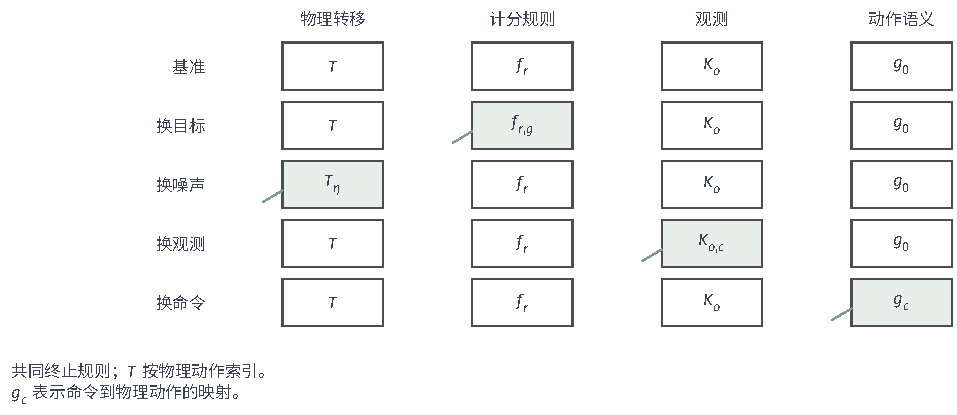
\includegraphics[width=161.988mm]{figures/10-reinforcement-learning/03-task-expansion-and-trustworthiness/tikz/rl-transfer-components.pdf}
  \caption{导航任务族的要素矩阵。相同符号与底纹表示同一分量，斜线及新符号表示变化；“换目标”行使用共同终止规则。$f_r(s,a,s')$表示给定转移后的计分规则，换目标时改为$f_{r,g}$；换噪声保留$f_r$，却可能改变均值奖励$R_c(s,a)$。$T$按物理动作索引，$g_c$把任务$c$的命令映为物理动作，基准接口记为$g_0$；若按命令标签索引，转移核也须相应变换。矩阵为控制变量设计，不表示已由交互记录证实共享关系。}
  \label{fig:rl-transfer-components}
\end{figure*}

图中不变的分量对应一项\term{共享结构}（shared structure）假设，即明确哪些任务对象具有可共同使用的关系。例如，统一状态动作语义后可以要求$T_c=T$；也可以要求奖励由同一组特征线性组合，观测映射到不混淆目标任务中不同最优动作的共同状态，或技能具有相同启动集与终止含义。每项假设约束的对象不同，强弱也不同。“任务相似”不能代替这些可检查的关系。

实验者编写的任务生成器可以保证某个模块不变，此时结构是已知的。若从训练任务的交互记录估计共同转移，再用未参与拟合的留出评价样本检验，则结构是估计结果，带有覆盖与误差条件。仅因两条学习曲线相似而猜测可以共享，只是待检验假设。控制变量比较应在相同状态、相同物理动作及相同反馈定义上检查差别；否则观测编码错误可能被误诊为动力学变化。

相似特征与相似回报都只能提供线索。一个编码器可能把两个外观相近、却需要相反动作的状态合并；两项任务也可能恰好在当前策略访问的区域一致，而在未访问区域完全不同。共同结构的声明必须带上适用状态动作范围。

% Outline: 6.2.2
\subsection{由共享结构确定可复用知识}
\label{sec:rl-transfer-objects}

即使已经确认两项任务的物理移动规律相同，也不能把所有旧参数一股脑儿保留。原因在于不同的学习对象依赖的条件不同：转移模型只预测“给定状态动作后会怎样变化”，只要完整转移与接口不变，它就可能继续适用；价值函数则在此之上还按奖励给这些变化打了分，奖励一变通常就得重算；策略直接选动作，即使动作仍能合法执行，也未必会走向新目标。因此复用要沿每个预测或决策规则的依赖条件逐项判断，而不能按整个网络文件笼统决定“用”还是“不用”。

例如，把终点从$(1,3)$换到$(4,1)$，可保留物理地图与动作效果，但到旧终点的距离和价值不能直接解释新任务。把滑移概率由基准的$0.2$改成教学假设$0.4$，目标坐标仍有相同含义，但旧到达概率必须重新估计。表~\ref{tab:rl-transfer-objects}~将复用对象与所需条件成对列出。

\begin{table*}[t]
  \centering\small
  \begin{tabularx}{\linewidth}{@{}>{\raggedright\arraybackslash}p{21mm}*{3}{>{\raggedright\arraybackslash}X}@{}}
    \toprule
    复用对象 & 共享条件 & 目标任务仍需估计的量 & 典型失效\\
    \midrule
    状态表示 & 保留会改变目标任务动作选择的状态差别；观测可对齐 & 任务特定变量、价值或策略 & 丢掉新目标需要的线索\\
    环境模型 & 相同转移机制或已知模块关系 & 风向、摩擦等特定参数 & 未建模机制改变\\
    奖励特征 & 特征语义不变，新奖励可表示 & 新权重$\bm w_c$ & 新目标不在特征类中\\
    后继表示与特征 & 固定策略、动力学和折扣 & 新奖励权重；必要时补新策略 & 转移变化或策略库覆盖差\\
    价值函数 & 原价值对应目标奖励、转移与策略 & 不满足条件时需重估价值 & 旧数值仍可算但含义已错\\
    策略初始化 & 接口兼容，少量更新有合适方向 & 目标任务参数修正 & 少量目标样本的估计波动导致负适应\\
    技能 & 启动集、可读状态或观测历史、动作效果和终止兼容 & 高层选择、组合或内部适应 & 能启动却不能达到所需效果\\
    \bottomrule
  \end{tabularx}
  \caption{可复用知识及其条件。共享条件说明对象何时有意义，不承诺从有限任务及其交互记录中训练出的模型满足这些条件。来源为本章定义与后文推导的归纳。}
  \label{tab:rl-transfer-objects}
\end{table*}

表中的技能还包含何时交还控制权。它是一段有内部策略和终止条件的持续行为，不是固定长度的动作数组。“绕过障碍”在新任务中可能仍能执行，但若新目标要求中途停在障碍旁，原终止条件就会错过需要的位置。因而要检查启动集、可读状态或观测历史、控制效果和终止条件是否仍服务于新决策，而不只是运行时有没有报错。第~\ref{chap:rl-learning}~章已定义单任务中的时间抽象，这里增加的是这些条件跨任务保持的要求。

% Outline: 6.3
\section{可复用决策知识的适用任务}
\label{sec:rl-transfer-applicability}

选定了复用对象，还必须限定它到底能面对哪些目标任务。同一个旧转移模型，可能适用于只换奖励的任务，却不适用于换了风向的任务；目标条件策略也只有在新目标描述有可解释语义时才能用。下面依次从任务生成关系、奖励变化、动力学变化、观测动作接口变化四个角度检查复用条件；同一个目标任务可能同时涉及其中几项。

% Outline: 6.3.1
\subsection{训练任务与目标任务的生成关系}
\label{sec:rl-transfer-distributions}

从同一目标和风向下多走几次，增加的是该任务的经历；另换目标或风参数，才增加了任务层的变化。要评价多任务训练的平均损失，需要把这两层随机性分别计算。用$p_{\text{训练}}(c)$表示训练任务总体分布，$p_{\text{目标}}(c)$表示声明的部署任务分布。给定$c$及行为策略$\beta$后，理论轨迹$\tau$的分布记为$P_{\mathcal E_c}^\beta$，在当前离散表示或共同支配测度下用$p_c^\beta$表示其质量函数或密度。协议实际取得的是可见记录$Z=b_c(\tau)$，其分布为$P_{\mathrm{rec},c}^\beta$；记录字段包括获准采集的状态或观测、动作、奖励与终止标记。轨迹律由初始分布、转移、观测与奖励和终止反馈的联合规律，以及行为策略共同决定；$R_c$只给出奖励均值，不能代替反馈分布。只拟合$(s,a,s')$时可以边缘化其余字段，但损失或采集策略用到的反馈必须保留。先在同任务内对轨迹取平均，再按训练任务的抽取概率平均：
\[
  \mathbb E_{c\sim p_{\text{训练}}}
  \mathbb E_{\tau\sim p_c^\beta}[\ell(c,\tau)].
\]
内层期望回答某项任务的平均损失，外层期望回答训练总体如何给各任务加权。用可见记录估计这个期望，还要求损失可由$Z$计算，或另有从记录识别损失期望的条件。即使一项任务内有大量轨迹，也没有因此获得其他目标或风向下的证据。

有限任务清单$\{c_1,\ldots,c_n\}$只给出了实际训练对象。任务生成器是可继续采样新对象的程序，其采样规则定义一个分布。理论中的总体分布则可能是对部署环境的假设，并不一定有可运行生成器。使用经验分布$n^{-1}\sum_i\delta_{c_i}$时应明确它只在已见任务上有质量，不能把这个支持集与假设总体的支持混用。

任务与轨迹的采样规则确定经验从哪里来，执行时还须另行声明任务参数$c$是否可见。用$c$指定MDP分量的设定称为\term{上下文MDP}（contextual MDP）；这里的上下文是任务条件，不一定是网络的历史窗口。物理状态与$c$都可见时，策略可直接写为$\pi(a\mid s,c)$。若物理状态可见、$c$隐藏且在适应期间固定，就需要保留各候选任务在已见历史下的概率$b_t(c)$。在给定正确任务模型和先验时，$(s_t,b_t)$构成\term{贝叶斯自适应MDP}（Bayes-adaptive MDP）的状态：它同时描述当前位置和对任务的认识，动作既改变位置，也产生更新认识的证据。物理状态也隐藏时，还须对状态与任务维护联合信念，第~\ref{sec:rl-transfer-belief}~节将展开更新。

图~\ref{fig:rl-transfer-task-plane}~给出一组教学任务划分。横轴为地图上边界目标$(x,3)$的横坐标，纵轴为总滑移概率$\eta$。训练总体仅允许$x\in\{1,2,3\}$，其中$x=3$只与$\eta\leq0.2$组合；$x=1,2$允许$0\leq\eta\leq0.4$。抽到一个未见的$(1,0.15)$仍属于同分布新任务；$(2,0.2)$可检验已见噪声值之间的插值；$(3,0.3)$的两个因素各自出现过，却在联合支持之外；$(4,0.45)$则含未见因素范围。

\begin{figure}[htbp]
  \centering
  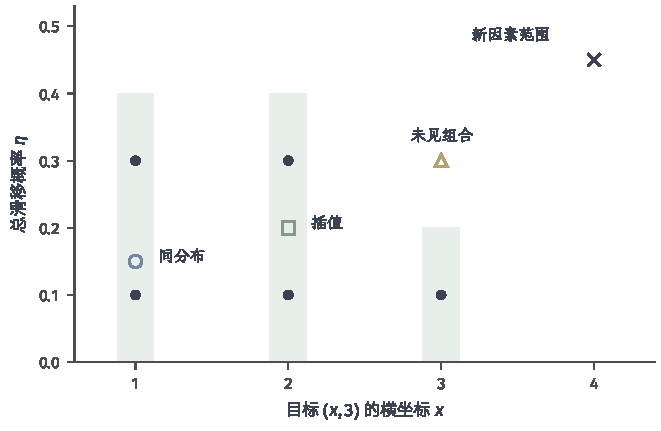
\includegraphics[width=112.000mm]{figures/10-reinforcement-learning/03-task-expansion-and-trustworthiness/matplotlib/rl-transfer-task-plane.pdf}
  \caption{目标位置与移动噪声的教学任务平面。竖向浅带表示离散目标坐标下的总体噪声支持，实点为有限训练样本，其他点形区分留出任务类型。插值只沿噪声轴解释，不把离散网格目标当成连续位置；所有点与支持范围均为教学设定。}
  \label{fig:rl-transfer-task-plane}
\end{figure}

这里“未见”相对于有限样本，“支持外”相对于声明的总体，二者不是同义词。若原总体本来就独立抽取目标与噪声，$(3,0.3)$可能只是在训练清单中缺席，而不在总体支持之外。组合测试必须说明所依据的是边缘支持、联合支持还是经验清单。

% Outline: 6.3.2
\subsection{目标与奖励变化下的可复用知识}
\label{sec:rl-transfer-reward-change}

先单独改变奖励：保持地图、移动规律和终止规则，只把沿途地标的得分换掉。旧转移模型仍可用于规划，旧价值却已经按原奖励计过分，不能直接解释新任务。若希望复用已有轨迹的长期后果，我们可以先记录经过哪些地标、付出多少步成本，再由新任务分别给这些事件赋权。

为使重新赋权可计算，设所有任务有共同$S,\mathsf A,T,\gamma$以及一致的观测、动作和终止语义。用共同的$d$维特征$\bm\phi(s,a,s')$记录一次转移中的事件，用$\bm w_c$记录任务$c$给各事件的权重。如果奖励属于这组特征的线性组合，就有
\begin{equation}
  R_c(s,a,s')=\langle\bm\phi(s,a,s'),\bm w_c\rangle,
  \qquad \bm\phi,\bm w_c\in\mathbb R^d.
  \label{eq:rl-transfer-linear-reward}
\end{equation}
内积把每个事件特征乘以对应权重再求和，因而把不变的事件描述与变化的评价规则分开。$R_c(s,a,s')$是给定这次转移后的期望奖励；再按后继状态概率平均，才得到$R_c(s,a)=\mathbb E_{s'\sim T(\cdot\mid s,a)}R_c(s,a,s')$。奖励样本$r_t$仍可有随机性，不能把上述期望当作每次实际反馈。

在固定策略下，保存未来各特征的期望折扣总量，就能用新权重重新计分。这一对象称为\term{后继特征}（successor features, SF）。对于教学路径，若前两步分别出现$\bm\phi_0=(1,0)^\top$、$\bm\phi_1=(0,1)^\top$，之后特征为0，那么$\gamma=0.9$时后继特征为$(1,0.9)^\top$；权重$(2,-1)^\top$给出价值$1.1$，换为$(0,3)^\top$则给出$2.7$。变化的是评价标准，而不是路径分布。

这个重新计分的例子固定了路径分布。若把得分地标改成一到达就吸收的新终点，后续访问也会改变，旧后继特征就不能直接使用。可以保留固定吸收出口而只改地标奖励，或重新学习包含新终止机制的后继特征。第~\ref{sec:rl-transfer-value-training}~节将从折扣求和推导这种分解，并说明多条已有策略的后果如何用于逐状态选动作。原始后继特征框架研究的也是共同动力学下的奖励迁移\scite{rl6-barreto2017-successor}

即使新奖励可表示，策略库也可能没有掌握通往新目标的行为。保存了正确的后果表示，只能评价已有行为及其可用组合，不等于已经拥有新任务的最优行为。

% Outline: 6.3.3
\subsection{动力学变化下的可复用知识}
\label{sec:rl-transfer-dynamics-change}

现在固定终点和计分规则，只改变移动噪声。进入终点仍得1，但窄路上的滑移可能使原路线更难到达。若这种变化都由一个风参数$\eta$控制，可以保留碰撞规则和模型族$T_\eta$，重新确定参数：$\eta$已给出时直接代入规划，$\eta$未知时用反馈估计。这样复用的是模型结构，不是原来那一组转移概率。

例如，在没有边界或障碍干扰的测试位置，偏离意图可以从后继位置直接辨认。令其指示量$X_j\sim\operatorname{Bernoulli}(\eta)$，独立重置采样$n$次后，用偏离比例$\widehat\eta=n^{-1}\sum_jX_j$估计风参数。独立性使和的方差等于$n\eta(1-\eta)$，取平均再除以$n^2$，所以估计方差为$\eta(1-\eta)/n$。把该参数用于全图，还需要风机制处处相同，并正确合并撞墙后留在原位的概率。墙边的不同滑移可能产生相同后继位置，此时反馈未必能直接给出$X_j$，不能照搬偏离次数估计。

共享模块可以表达“几何碰撞规则相同，风模块变化”；平滑模型可以要求，在指定参数范围内，$\eta$的差异趋于0时，同一状态动作下转移分布的$\ell_1$差异也趋于0。前者减少重复估计的对象，后者给出参数插值的依据；要得到数值误差界，还须限定参数差能使转移差增大多少，两者都不是从网络参数共享自动推出的事实。一般有限表格转移要估计约$|S||\mathsf A|(|S|-1)$个自由概率，单个风参数只估计一个量，但这个维数比较不包含辨识它所需的访问成本。

反例更直接：在同一可见岔路，两个动作分别通向奖励1和0的区域；第二个任务将两个动作的物理效果互换，图像与奖励标记完全不变。旧策略仍选原来的动作，回报由1变为0。旧后继特征预测它会访问奖励区域，因而同样失效；仅修改奖励权重不能把错误转移改对。这个单步例是从导航提取的教学简化，取消滑移与步成本。

即使新旧转移接近，也要检查这种单步误差对长期价值的影响。固定同一策略$\pi$，在共同状态动作空间上比较$T_c$和$T_{c'}$，先假设两者有相同的条件期望奖励$R(s,a)$且$|R|\leq R_{\max}$。以$\sup_{s,a}\lVert T_c-T_{c'}\rVert_1\leq\delta$限制所有相关状态动作上的转移差异；取上确界是为了防止某个策略会访问的位置被平均误差掩盖。两条Bellman关系相减后，继续价值之差贡献第一项，转移之差作用于有界价值贡献第二项：
\[
 \lVert V_c^\pi-V_{c'}^\pi\rVert_\infty
 \leq \gamma\lVert V_c^\pi-V_{c'}^\pi\rVert_\infty
      +\gamma\delta\,\frac{R_{\max}}{1-\gamma}.
\]
这里使用了$\lVert V_{c'}^\pi\rVert_\infty\leq R_{\max}/(1-\gamma)$，以及转移概率差作用于有界函数时的$\ell_1$界。把第一项移到左侧，再除以$1-\gamma$，得到$\gamma\delta R_{\max}/(1-\gamma)^2$。折扣越接近1，越远的后果进入评价，单步差异也可能积累得越大。

共同计分规则不一定给出共同均值奖励。“进入终点得1”虽未改变，到达概率变化仍会改变$R_c(s,a)$。若两者都受同一$R_{\max}$约束，价值界还须加入$\lVert R_c-R_{c'}\rVert_\infty/(1-\gamma)$。这些界限定的是固定策略及全相关状态动作上的误差，训练参数范围内较小的平均预测误差既不能替代一致界，也不能证明范围外参数仍满足它。

% Outline: 6.3.4
\subsection{观测与动作接口变化下的可复用知识}
\label{sec:rl-transfer-interface}

把地图颜色换掉，并不一定改变小车的物理位置；交换左右动作标签，则会改变同一输出命令的控制效果。对一段“右、右、上”的命令序列，单纯换色后物理轨迹可以完全不变，交换命令后却可能向相反方向移动，甚至使命令不再合法。因此观测编码与动作命令应分别对齐。

要判断换接口后是否仍是同一个控制问题，可以比较对应状态上执行对应动作的后果。设$e_c(o)$把新观测编码成原策略所需的决策表示，$m_c(a)$把原语义动作$a$转换成新环境命令，$f_c$把新任务状态对应到原任务状态。这里$m_c$与图\ref{fig:rl-transfer-components}中的$g_c$具有不同方向：$m_c$把原策略动作映为新命令，$g_c$再把新命令映为物理动作。若两任务使用同一物理动作集合，保持物理效果要求$g_c(m_c(a))=g_0(a)$；这只要求在复用动作范围内找到相匹配的命令，不要求$g_c$为双射或存在全局逆。下式的$T_0,T_c$按各自环境的命令索引，已包含相应命令的物理效果。对原任务中的任意相关后继集合$B$，$f_c^{-1}(B)$收集映射到$B$的新任务状态。一个精确复用的充分条件是奖励保持，并且到达这些对应集合的概率相等：
\[
 T_c\!\left(f_c^{-1}(B)\mid s,m_c(a)\right)
 =T_0\!\left(B\mid f_c(s),a\right)
\]
等式需对所有相关状态、合法动作和后继集合$B$成立，还要由$e_c$保留会改变目标动作选择的观测差别、由$m_c$保持动作合法性。左侧在新任务执行映射后的命令，右侧在原任务执行原动作；两者比较的是控制后果，而不是图像或向量的外观相似。图~\ref{fig:rl-transfer-interface}~把观测编码、策略决策、命令映射和执行分别标出。

\begin{figure*}[t]
  \centering
  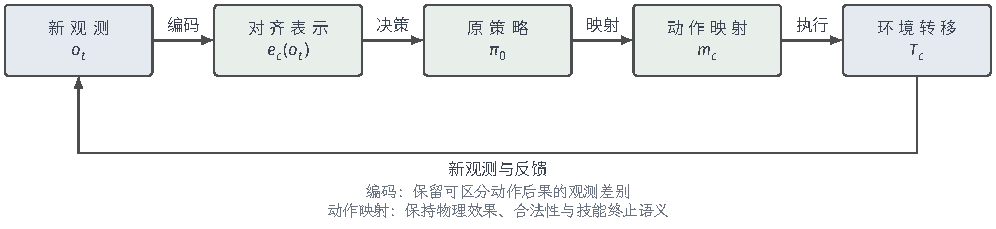
\includegraphics[width=168.575mm]{figures/10-reinforcement-learning/03-task-expansion-and-trustworthiness/tikz/rl-transfer-interface.pdf}
  \caption{观测和动作接口的迁移。观测编码需要保留动作后果预测所需的状态差别，命令映射需要保留物理效果与合法性；任何一侧缺少对应关系，原策略都不能原样解释新接口。图为上述充分条件的原创结构示意。}
  \label{fig:rl-transfer-interface}
\end{figure*}

对于技能，还要把启动状态映射到原启动集，把“到达出口”映射到相同的终止事件。只映射原始动作，而忽略技能结束条件，可能导致高层策略等待一个永远不会到来的反馈。

有限日志未必能唯一确定这些映射。若日志只记录“上”和“下”，左右动作交换前后与全部记录相容；图像重建也无法辨认未试过命令的含义。需要增加有区分力的动作记录，或者提供可信的接口说明。控制充分表示与目标量可识别性的区别见第~\ref{chap:rl-information}~章：同尺寸接口、感知相似度和重建成功都不够。

% Outline: 6.3.5
\subsection{组合与支持外任务所需的额外假设}
\label{sec:rl-transfer-composition}

训练时见过“远终点、无风”和“近终点、有风”，并不意味着已经见过“远终点、有风”。若目标模块只改变奖励、风模块只改变转移，且二者接口独立，模型可以组合这两种知识；若有一个仅在远终点且有风时出现的障碍，原来的两项任务却完全不能揭示它。

把这一区别写成集合关系，令$c=(g,\eta)$。边缘支持$\operatorname{supp}(p_g)$、$\operatorname{supp}(p_\eta)$分别表示总体允许哪些目标和风参数；联合支持$\operatorname{supp}(p_{g,\eta})$表示总体允许哪些目标与风的配对。一个允许配对的两个分量必然各自允许，所以
\[
 \operatorname{supp}(p_{g,\eta})
 \subseteq \operatorname{supp}(p_g)\times\operatorname{supp}(p_\eta),
\]
反向包含不一定成立，两个各自允许的分量未必能配对。\term{组合泛化}（compositional generalization）是在已学因素之间使用未见配对，而不只是识别每个因素。其依据可能是$T_c=T_\eta$、$R_c=R_g$等因子分解，但还需保证组合后观测、动作和终止接口仍成立；这些关系不能由两个单因素测试自动推出。

可以构造两个生成器：它们在已见组合上给出完全相同的地图，只在“远且有风”时分别保持通路或封闭通路。任何只用现有训练组合的算法面对两者取得同分布的训练交互记录，因而不能仅凭这些记录确定新组合是否可通行。增加同一组合的轨迹数量无法消除这个歧义。

未见组合仍由已见因素组成；若引入训练范围外的新动作效果，就连该因素怎样作用于环境也没有从已有训练任务的交互记录中确定。要进一步外推，需要可识别的机制、适用范围明确的平滑性或结构不变性。测试应分别留出组合和因素范围，才能知道支持的是哪一种能力；任务数量多本身并没有给出这些结构关系。

% Outline: 6.4
\section{可复用决策知识的训练}
\label{sec:rl-transfer-training}

前面回答了“什么可以复用、复用到哪里”，接下来要回答“怎样从经验中把这些可复用的知识学出来”。例如多种风向下收集的状态转移记录可以训练一个以风为条件的转移模型，多目标轨迹可以训练一个以目标为条件的价值函数，但两者拟合的对象并不相同。可学习的对象包括表示、模型、价值和策略；而任务随机化、条件化、蒸馏、目标重标记等则是将任务、交互记录或教师动作分布用于这些训练目标的手段，可以组合使用，但都仍受前面共享条件与任务支持的约束。

% Outline: 6.4.1
\subsection{训练任务与经验的构造}
\label{sec:rl-transfer-data}

训练导航任务时，可以随机抽取目标坐标和风强度，也可以用程序生成地图；后者还需检查连通性、合法动作和终止规则。任务产生后，仍要由收集策略真正走出轨迹。因此，训练记录的采样分成两层：按$q(c)$抽任务，再由任务内策略$\beta_c$访问状态动作。折扣采样下，用归一化占用度量$d_c^{\beta_c}(s,a)$描述访问概率，联合经验权重便是$q(c)d_c^{\beta_c}(s,a)$。提高某任务的抽取频率只改变第一个因子，不保证它的关键窄路已被充分访问。

改变$q$还改变了各任务对损失的贡献。若希望保留$p_{\text{训练}}$下的平均目标，就需要用概率或密度比$p_{\text{训练}}(c)/q(c)$重新加权，使按$q$采样的期望恢复为所需期望。这要求$p_{\text{训练}}$相对于$q$绝对连续，即训练目标允许的任务不能落在$q$从不采样的范围；离散时，每个$p_{\text{训练}}(c)>0$的任务都须有$q(c)>0$。重加权不能补回未采任务，过大的权重还会增加估计方差。课程学习若偏向当前较难的任务，应报告这种目标权重变化，不能只描述为增加训练次数。这里的密度比只恢复同一任务条件目标的外层权重，不校正任务内行为策略改变造成的轨迹分布差异。共享条件和绝对连续性成立时，重要性加权可以变换期望的积分分布；有限样本保证还须控制权重大小、损失矩及实际采样依赖。相关跨分布分析可参考\BookChapterRef{chap:transfer-learning-theory}{卷3《基础、理论与可信性》“迁移学习的可学习性”章}。

有些失败轨迹无需重新交互，就能回答另一个目标的问题。\term{事后经验回放}（hindsight experience replay, HER）把轨迹实际达到的位置当作替代目标，重算该目标下的反馈，再交给离策略学习器。它重新解释了已经发生的转移，没有制造另一条物理轨迹\scite{rl6-andrychowicz2017-her}

例如，教学轨迹从$(1,1)$出发，依次到达$(2,1)$、$(3,1)$和$(4,1)$，没有到达原目标$(4,3)$。用新目标$g'=(3,1)$，设到达目标得1、之前每步得$-0.04$，则前两条转移的奖励由$(-0.04,-0.04)$改为$(-0.04,1)$。若新任务到达目标立即结束，第二条转移的终止标记必须同时改为1，后续从$(3,1)$继续移动的记录不能接在这条新回合后作为有效经验。图~\ref{fig:rl-transfer-relabel}~区分真实采集与离线重标记。

\begin{figure*}[htbp]
  \centering
  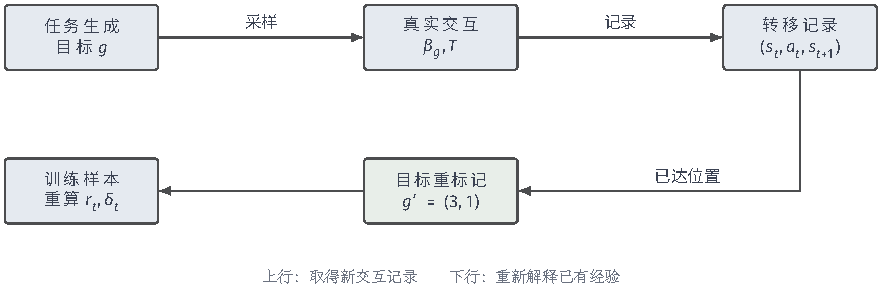
\includegraphics[width=149.296mm]{figures/10-reinforcement-learning/03-task-expansion-and-trustworthiness/tikz/rl-transfer-relabel.pdf}
  \caption{任务生成与目标重标记的两条训练记录构造路径。上行产生真实轨迹，下行重算已有轨迹的目标、奖励和终止标记；重标记箭头不回连环境，因而不增加真实状态动作覆盖。原理据HER，具体导航路径为本章教学构造。}
  \label{fig:rl-transfer-relabel}
\end{figure*}

重标记的语义有效性至少要求：目标不改变非终止物理转移，奖励及目标相关终止信号可按记录重算，动作在新解释中仍合法。若开门目标同时改变门是否锁住，就不能把旧转移当作新目标样本。即使语义有效，随机环境中的选择偏差仍是另一个问题。

设教学单步任务的同一个动作以各$1/2$概率落在左、右地标，且目标不影响转移。真实左目标下成功概率为$1/2$；如果只把“实际落在左边”的记录重标成左目标，再用这些记录估计该动作的左目标成功率，就得到1。每条保留记录都可能真实发生，但条件选择删除了失败分支。确定性动力学可避免这种特定的随机结果选择问题，随机环境则需检查重标记分布或采用适当校正；“目标不改变转移”本身不能证明估计无偏。

重标记$m$个目标会把每条原始记录扩成至多$m$条训练记录，奖励重算约需$O(m)$次调用。增加的是训练计算与目标覆盖，不是$m$倍独立环境证据。

% Outline: 6.4.2
\subsection{可复用状态表示的训练}
\label{sec:rl-transfer-representation-training}

在多个任务间共享一个状态表示，看似总能节省学习，实际上需要小心一个陷阱。不同终点的任务都需要辨认障碍的位置，障碍位置与地图几何可以共享；但在同一个岔路口，它们可能需要截然相反的动作。如果价值或策略只收到相同的观测表示，又没有目标坐标或任务描述作为其他条件，就无从区分该往哪走。因此所谓“任务不变表示”只要求共同的控制要素保持一致，而不要求不同任务的观测与目标描述被压成同一表示；那些会改变动作选择的任务变量，必须在编码器或其后的价值、策略中留有入口。

这个入口可以放在不同位置。共享编码器$\bm z=e_{\bm\theta}(o)$只处理观测，由后续价值或策略另接任务描述$c$；任务条件表示$\bm z=e_{\bm\theta}(o,c)$在编码时就使用目标。模块化表示$\bm z=(e_{\bm\theta}(o),e_{\bm\omega_c}(o,c))$则把共同几何与任务特定的观测编码或转移特征分开，其中$\bm\omega_c$是特定模块参数。三者都可向$Q(\bm z,a,c)$、$\pi(a\mid\bm z,c)$或潜在转移模型供给表示，表~\ref{tab:rl-transfer-representations}~在这些共同用途下比较共享位置与训练条件。

\begin{table*}[t]
  \centering\small
  \begin{tabularx}{\linewidth}{@{}>{\raggedright\arraybackslash}p{18mm}*{5}{>{\raggedright\arraybackslash}X}@{}}
    \toprule
    设计 & 共享部件 & 任务特定部件 & 训练信号 & 任务权重 & 适用条件\\
    \midrule
    共享编码器 & 感知与几何表示 & 条件头或独立头 & TD误差、策略梯度、预测 & 显式$q(c)$ & 编码未混淆目标任务需区别对待的观测\\
    条件表示 & 编码规则和参数 & 描述$c$或历史变量 & 条件价值、控制与预测 & 相同总量下检查各任务 & 描述语义及条件支持兼容\\
    模块化表示 & 共同子模块及组合器 & 风、传感器等模块 & 模块预测与端到端控制 & 可按模块或任务平衡 & 分解与组合接口成立\\
    \bottomrule
  \end{tabularx}
  \caption{三种表示设计。训练信号可以组合，但“参数共享”只描述实现，不能替代控制充分性证明。各列为本章机制归纳。}
  \label{tab:rl-transfer-representations}
\end{table*}

以共享编码器接入评论家为例，训练要让当前动作价值与一步反馈加继续价值一致。一条经验给出的目标为
\[
  y_t=r_t+\gamma(1-\delta_t)
      \max_{a'}\overline Q(e_{\overline{\bm\theta}}(o_{t+1}),a',c).
\]
其中$\delta_t$表示任务真正终止，最大值在后继状态的合法动作中比较继续回报；终止后不再自举。最小化$\tfrac12(Q(e_{\bm\theta}(o_t),a_t,c)-y_t)^2$惩罚当前预测与该目标的残差，梯度通过评论家进入编码器，目标网络在此次梯度中固定。重建损失可帮助感知，但重建成功不等于仍能区分会改变动作后果的观测；还需结合控制目标和充分性条件检查哪些动作后果能被区分。

在一个教学单步岔路中，目标左与目标右需要相反动作。若两项任务的价值或策略接收完全相同的决策表示，任何确定策略都只能满足其中一项；加上一个目标位即可消除这个表示冲突。另一方面，若左任务占采样的$90\%$，总体正确率$90\%$的常向左策略可能完全放弃右任务。这是任务权重造成的平均优势，不是两项任务都获得迁移。

训练计算随编码器前后向成本和样本数增长；多头设计还随任务头数量增加存储，模块化则增加组合与路由成本。诊断时应报告分任务回报、目标位消融与匹配容量的独立模型，区分关键观测差别被抹去、容量不足和优化冲突。总体损失下降不能回答这些不同问题。

% Outline: 6.4.3
\subsection{可复用环境模型的训练}
\label{sec:rl-transfer-model-training}

同一地图上不同风向的轨迹，都受到共同碰撞几何约束，却有不同偏移概率。模型可让共享模块处理几何，再由任务变量确定偏移。令$\widehat T_{\bm\theta,\bm\omega_c}(s'\mid s,a,\bm z_c)$预测下一状态的分布，其中$\bm\theta$为共享参数，$\bm\omega_c$为可选任务特定参数，$\bm z_c$来自描述或历史推断。若另学条件期望奖励与观测分布，分别用$\widehat R$和$\widehat K_o$表示。$\widehat R$预测奖励的条件均值，不是奖励概率分布；生成完整反馈还须规定奖励分布及其与后继状态、观测、终止标记的联合关系。仅拟合转移并没有得到包含全部反馈的模拟器。

在完全可观测、有限离散状态的长度$H$轨迹上，可以检查模型给真实后继状态多大概率。训练提高记录中各步条件转移概率的乘积，等价于最小化负对数似然；对数把各步概率的乘积变成和，负号使低概率预测受到较大惩罚。先对一条轨迹的$H$步平均，再按任务抽样$q$和收集策略的轨迹分布平均，得到
\begin{equation}
 \mathcal L_{\text{模型}}
 =\mathbb E_{c\sim q}\mathbb E_{\tau\sim p_c^{\beta_c}}
 \left[-\frac1H\sum_{t=0}^{H-1}
 \log\widehat T_{\bm\theta,\bm\omega_c}
 (s_{t+1}\mid s_t,a_t,\bm z_c)\right].
 \label{eq:rl-transfer-model-loss}
\end{equation}
模型以已记录的$s_t,a_t$为条件，只拟合后继分布，不把收集策略的动作概率拟合成动力学。经验目标用采到的任务和轨迹平均近似上述期望，再对模型参数求梯度。本式固定$H$并按任务平均；若回合长度不同，按回合平均和按步平均会给任务不同权重，需要另行选定。在相同训练样本、采样分布和权重下，较低训练负对数似然表示模型在这一评分上的改善，尚不能证明模型在未访问位置也正确。

图~\ref{fig:rl-transfer-model}~展示共同几何与任务条件模块如何组合。完全共享模型相当于忽略$\bm\omega_c,\bm z_c$；完全独立模型则为每项任务各拟合全部参数。模块化减少的是共同几何的重复估计，仍需估计新风向，不能以共享参数比例推算目标样本效率。

\begin{figure*}[htbp]
  \centering
  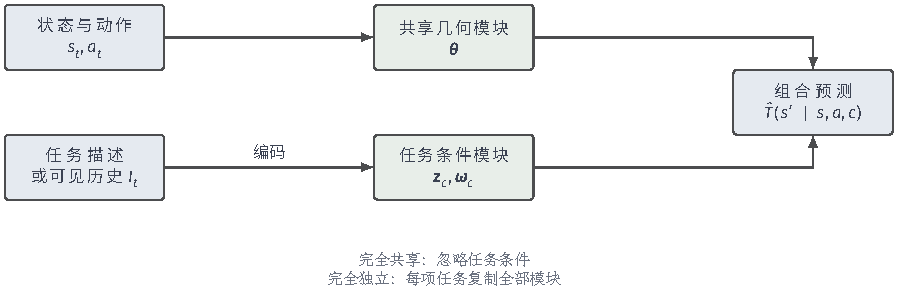
\includegraphics[width=151.987mm]{figures/10-reinforcement-learning/03-task-expansion-and-trustworthiness/tikz/rl-transfer-model.pdf}
  \caption{任务条件环境模型。状态动作进入共享模块，描述或历史进入任务模块，两者共同决定转移预测；奖励、观测头仅在确实训练时增加。图为本章模型参数化的原创示意，不表示所有环境都满足这种分解。}
  \label{fig:rl-transfer-model}
\end{figure*}

用前述一维风参数检验这个目标。在8次可辨认滑移的独立教学试验中观察到2次偏离，似然为$\eta^2(1-\eta)^6$，负对数似然便是$-2\log\eta-6\log(1-\eta)$。在$0<\eta<1$内令导数$-2/\eta+6/(1-\eta)=0$，得到$\widehat\eta=1/4$；目标在两端趋于无穷且二阶导数为正，因此该点是最小点。随后把估计送入共同碰撞模型，计算各位置转移；从测试位置扩大到全图，仍依赖同一个风参数处处适用的结构假设。

训练时知道$c$，部署时却只有历史，是一个额外推断问题。应训练从可见历史到$\bm z_c$的编码器，并在测试中只给这些历史；不能把真实风标签作为隐蔽输入。固定日志上的训练成本约为训练记录数乘单样本模型前后向成本，模型内规划还要乘候选动作序列数及前瞻深度。未覆盖风向、传感器变化和反复滚动的误差累积，都可能使训练似然较好的模型产生错误策略。

% Outline: 6.4.4
\subsection{可复用价值与策略的训练}
\label{sec:rl-transfer-value-training}

表示和转移模型确定之后，还需要按目标来评价动作。同一个岔路通往不同终点时，“向左好不好”取决于要去哪里，因此价值的输入里必须含有目标$g$。如果为每个目标单独存一张价值表，目标一多就无法承受，也无法推广到没见过的目标。\term{通用价值函数逼近器}（universal value function approximator, UVFA）的做法是用一个函数$Q_{\bm\theta}(s,a,g)$统一表示不同状态、动作和目标下的价值；目标条件MDP把$g$纳入任务描述，使这一输入有明确含义\scite{rl6-schaul2015-uvfa}。

训练时从任务$g$的行为策略取得转移，按相同目标确定奖励和终止，再拟合TD目标$r_t+\gamma(1-\delta_t)\max_{a'}\overline Q(s_{t+1},a',g)$。其中最大值比较后继状态的合法动作，表示继续控制的最高估计回报；真正终止时继续项为0。当前预测与目标的残差用于更新参数，执行时也必须查询相同的$g$。多目标共同训练改变了拟合范围，没有取消TD学习的覆盖和估计条件。

实现这种条件价值时，可以由共享评论家联合表示所有目标，也可以共享特征、为各已见任务设置独立输出头；模块化策略则分别处理几何、目标或控制模式。多头的任务编号本身不能解释新目标，UVFA接受连续坐标也不保证能外推到未训练范围。每次TD更新要计算当前价值和目标动作值，有限动作枚举成本随$|\mathsf A|$增长；连续动作不能逐一枚举，需要行动者或其他最大化近似。

条件价值仍需学习不同目标的计分结果。若希望按新奖励重用同一策略的长期后果，可以先记录未来访问次数；这与前面后继特征的两步例子相连，这里进一步说明该记录怎样计算和训练。其前身\term{后继表示}（successor representation, SR）记录固定策略下未来访问各状态的期望折扣次数。有限状态时，$M^\pi(s,u)$描述从$s$出发对状态$u$的访问量：
\[
 M^\pi(s,u)=\mathbb E_\pi\!\left[\sum_{t\geq0}\gamma^t
       \mathbb I\{s_t=u\}\mid s_0=s\right].
\]
指示量只在访问$u$时计1，折扣和区分到达早晚，期望则平均策略与转移的随机结果。若$\bm T^\pi$为策略诱导的状态转移矩阵，拆出$t=0$时的当前访问，余下从下一状态继续，便得
$\bm M^\pi=\bm I+\gamma\bm T^\pi\bm M^\pi$，从而
$\bm M^\pi=(\bm I-\gamma\bm T^\pi)^{-1}$。矩阵的谱半径是其特征值绝对值的最大值；随机矩阵$\bm T^\pi$的谱半径不超过1。乘以$\gamma<1$后，$\gamma\bm T^\pi$的每个特征值绝对值都小于1，因而1不是它的特征值，0也就不是$\bm I-\gamma\bm T^\pi$的特征值。该矩阵因此可逆，方程给出确定的访问量。SR一般存储$|S|^2$个数；若只需重新评价特定事件，可以把每个状态的指示量换成低维事件特征，得到SF\scite{rl6-dayan1993-successor}

SF需要按当前动作比较价值，因此条件中固定首动作$a$，此后再遵循$\pi$。下面对所有相关转移限制特征范数，保证无限折扣和有界；这个上确界条件是求期望和交换极限的依据，不是平均特征较小就能代替的条件。

\begin{definition}[固定策略的后继特征]
 \label{def:rl-transfer-sf}
 给定状态空间$S$、行动空间$\mathsf A$、非空合法动作集$\mathsf A(s)$及转移核$T$，各空间与核采用相容的可测结构，取共同折扣$0\leq\gamma<1$。令正整数$d\geq1$，可测特征映射$\bm\phi:S\times\mathsf A\times S\to\mathbb R^d$在所有合法转移上满足
 $\sup_{s\in S,a\in\mathsf A(s),s'\in S}\lVert\bm\phi(s,a,s')\rVert_2\leq C_\phi<\infty$。
 固定合法平稳Markov策略$\pi$，其中$\pi(\cdot\mid s)$是在$\mathsf A(s)$上的概率核；其后继特征为
 \begin{equation}
 \bm\psi^\pi(s,a)=
 \mathbb E_\pi\!\left[
 \sum_{t=0}^{\infty}\gamma^t\bm\phi(s_t,a_t,s_{t+1})
 \,\middle|\,s_0=s,a_0=a\right].
 \label{eq:rl-transfer-sf}
 \end{equation}
 首动作按条件强制执行，之后服从$\pi$。
\end{definition}

定义得到的是事件总量，还需证明它乘上权重后确实等于动作价值。对随机奖励，另假设各状态动作下的绝对一阶矩有共同有限上界；有界奖励样本是一个充分条件，这保证折扣奖励和可积。记$\bm\phi_t=\bm\phi(s_t,a_t,s_{t+1})$，由特征有界性，
$\sum_{t\geq0}\gamma^t\lVert\bm\phi_t\rVert_2\leq C_\phi/(1-\gamma)$；
对固定有限$\bm w_c$，条件期望奖励的绝对折扣和也有上界
$C_\phi\lVert\bm w_c\rVert_2/(1-\gamma)$。因此可以用支配收敛把部分和的极限移入期望，并用条件期望先把$r_t$替换成转移条件期望奖励。依次得到
\begin{align}
 Q_c^\pi(s,a)
 &=\lim_{N\to\infty}\mathbb E_\pi
       \left[\sum_{t=0}^{N}\gamma^t R_c(s_t,a_t,s_{t+1})
       \mid s_0=s,a_0=a\right]\notag\\
 &=\lim_{N\to\infty}\left\langle
       \mathbb E_\pi\left[\sum_{t=0}^{N}\gamma^t\bm\phi_t
       \mid s_0=s,a_0=a\right],\bm w_c\right\rangle\notag\\
 &=\langle\bm\psi^\pi(s,a),\bm w_c\rangle.
 \label{eq:rl-transfer-sf-value}
\end{align}
第二步使用式~\eqref{eq:rl-transfer-linear-reward}~与有限和、内积的线性性，第三步使用前述可积性。SF不含奖励权重，却仍依赖$T$和$\pi$；在新任务换掉转移后，原式右侧不再使用正确的轨迹分布。

价值分解解释了SF的用途，但完整轨迹求和不便于逐步训练。与标量价值一样，把首步特征和以后特征分开，利用马尔可夫性先平均后继状态、再按固定策略平均下一动作，就得到向量Bellman方程：
\begin{equation}
 \bm\psi^\pi(s,a)=
 \mathbb E_{s'\sim T}\left[\bm\phi(s,a,s')
 +\gamma\mathbb E_{a'\sim\pi(\cdot\mid s')}\bm\psi^\pi(s',a')\right].
 \label{eq:rl-transfer-sf-bellman}
\end{equation}
方程把长时程事件总量化成一步目标，可以用转移样本近似。表格情形从覆盖相关状态动作的行为策略$\beta$取得转移，计算
$\bm y_t=\bm\phi_t+\gamma\sum_{a'}\pi(a'\mid s_{t+1})\widehat{\bm\psi}(s_{t+1},a')$，
再令$\widehat{\bm\psi}(s_t,a_t)$向$\bm y_t$移动步长$\alpha$。终止时继续项为0。若仅采样一个$a'\sim\pi$，则以该样本替代动作期望。这里评价的是固定$\pi$，不能无说明地把下一动作改成最大值。表格每次更新的向量运算为$O(d|\mathsf A|)$，采样下一动作时为$O(d)$；网络实现还包含前后向成本。

SF训练不需要新奖励权重，但新任务计分需要它。若$\bm w_c$未知，可比较目标奖励样本$r_j$与特征预测$\bm\phi_j^\top\bm w_c$，最小化残差平方和
$\sum_j(r_j-\bm\phi_j^\top\bm w_c)^2$。平方惩罚预测偏差，样本和形成经验拟合目标；要使这项$d$维线性最小二乘拟合有唯一解，训练特征矩阵还需满列秩，有噪声时唯一拟合值仍不保证等于真实权重。若目标描述直接给出权重，则不需要这一步目标反馈，但仍须有共同动力学下训练好的SF。

有了多条策略的SF，就能按同一个新奖励计算各自的动作价值。固定调用一条策略可能错过另一条策略在某个状态的有用动作。\term{广义策略改进}（generalized policy improvement, GPI）在每个状态比较所有库内策略的动作价值，再选择估值最高的合法动作；动作执行后可以重新选择，不必整回合锁定同一条策略。先对策略取最大值，再对动作取最大值，是要利用库内任一策略提供的较高继续价值。下面的保证因此以已有策略为参照，不与未知的新任务最优策略比较\scite{rl6-barreto2017-successor}

\begin{theorem}[有一致估计误差的广义策略改进]
 \label{thm:rl-transfer-gpi}
 在同一个状态集$S$及各合法动作集$\mathsf A(s)$均有限且非空、逐步奖励有界、折扣$0\leq\gamma<1$的MDP中，取正整数$m$和$\varepsilon\geq0$，给定$m$条合法平稳Markov策略
 $\{\pi_1,\ldots,\pi_m\}$。若对每个$i=1,\ldots,m$及所有合法状态动作均满足
 $|\widehat Q^{\pi_i}(s,a)-Q^{\pi_i}(s,a)|\leq\varepsilon$，
 定义确定性策略的动作映射
 \[
 \pi(s)\in\argmax_{a\in\mathsf A(s)}\max_i\widehat Q^{\pi_i}(s,a),
 \]
 并固定平局规则；对应的策略核为该动作上的点质量，则
 \begin{equation}
 Q^\pi(s,a)\geq\max_iQ^{\pi_i}(s,a)
                -\frac{2\varepsilon}{1-\gamma}.
 \label{eq:rl-transfer-gpi-bound}
 \end{equation}
\end{theorem}

要证明逐状态拼接后仍有保证，先限制一次近似贪心选动作的损失，再沿Bellman备份累计它。令
$f(s,a)=\max_iQ^{\pi_i}(s,a)$、$\widehat f(s,a)=\max_i\widehat Q^{\pi_i}(s,a)$；
一致误差保证$|f-\widehat f|\leq\varepsilon$。由$\pi$的贪心定义，
\[
 f(s,\pi(s))\geq\widehat f(s,\pi(s))-\varepsilon
 =\max_a\widehat f(s,a)-\varepsilon
 \geq\max_a f(s,a)-2\varepsilon.
\]
两个$\varepsilon$分别来自所选动作的估值误差和最佳动作的估值误差。用$\mathcal B^\pi$表示动作价值的Bellman评价算子；下一状态按$\pi$选出的$f$值至多比最大值低$2\varepsilon$，平均并折扣后有
\begin{align*}
 \mathcal B^\pi f
 &\geq R+\gamma T\max_a f-2\gamma\varepsilon\\
 &\geq \max_i\{R+\gamma T\mathbb E_{a'\sim\pi_i}Q^{\pi_i}\}
           -2\gamma\varepsilon\\
 &=f-2\gamma\varepsilon\geq f-2\varepsilon.
\end{align*}
其中$T$表示对后继状态取期望；第二行用“每个后继状态上的最大值至少覆盖任一$\pi_i$的动作平均”，再对策略取最大。Bellman单调性以及
$\mathcal B^\pi(f-b)=\mathcal B^\pi f-\gamma b$给出
$(\mathcal B^\pi)^k f\geq f-2\varepsilon\sum_{j=0}^{k-1}\gamma^j$。
有限折扣MDP中，$\mathcal B^\pi$是压缩算子，左侧迭代收敛到$Q^\pi$；右侧几何级数收敛到$1/(1-\gamma)$，于是得到式~\eqref{eq:rl-transfer-gpi-bound}。损失容限来自一致估值误差的逐步积累。深度网络的平均TD损失较小，并没有因此满足全状态动作上误差至多$\varepsilon$的条件。

\begin{example}[两条绕障策略的新奖励评价]
 \label{ex:rl-transfer-sf-routes}
 以下简化保留导航地图与固定吸收出口$(4,3)$，取消滑移与步成本，沿途地标允许重复计分。取特征为进入$(1,3)$、进入$(4,1)$、首次进入出口的三个指示量，吸收后特征为0，$\gamma=0.9$。两条确定策略从起点分别走“上、上、右、右、右”和“右、右、右、上、上”；离开这两条路线的状态可用任一固定合法规则补全策略。

 上路在$t=1$经过第一个地标，$t=4$进入出口；下路在$t=2$经过第二个地标，$t=4$进入出口。因此从起点执行各自首动作并继续原策略时，
 \[
 \bm\psi^{\pi_1}=(0.9,0,0.6561)^\top,\qquad
 \bm\psi^{\pi_2}=(0,0.81,0.6561)^\top.
 \]
 新权重$\bm w=(1,2,1)^\top$给出两条完整路线的回报$1.5561$与$2.2761$。固定调用下路优于固定调用上路；GPI则需为每个候选首动作查询每条补全策略的SF，再逐状态选择，不能仅凭这两个整路线数字实现。

 当SF精确时，GPI在各状态不会劣于库内任一策略；当所有动作价值一致误差至多为教学假设$\varepsilon=0.01$时，本定理给出的逐动作损失容限为$0.2$。从状态开始执行GPI也满足同样的保守容限：近似贪心至多损失$2\varepsilon$，后续至多损失$2\gamma\varepsilon/(1-\gamma)$。这些保证没有比较库外最优策略；地标重复奖励甚至可能使有益循环优于直接离场。
\end{example}

策略库有$m$条策略、每个SF为$d$维时，直接GPI查询约需$m|\mathsf A|$个SF输出和$O(m|\mathsf A|d)$次乘加。相比每个新奖励都从头学习，它复用了后果计算；相比单次策略前向，它增加了查询成本。新奖励残差、新动力学误差和策略库缺失各自需要额外分析，不能全塞进未经测量的$\varepsilon$。

GPI保留多份后果表示，查询成本随策略库增长。如果部署希望用一个网络保存多个教师的已有行为，可以在教师访问的状态上拟合其动作分布，这称为\term{策略蒸馏}（policy distillation）。共同动作接口下，用教师分布到学生分布的KL散度衡量拟合差异，再按任务采样$q$和状态分布$\nu_c$平均：
\[
 \mathcal L_{\text{蒸馏}}=
 \mathbb E_{c\sim q,\,s\sim\nu_c}
 D_{\mathrm{KL}}\!\left(\pi_c^{\text{教师}}(\cdot\mid s)
       \,\Vert\,\pi_{\bm\theta}(\cdot\mid s,c)\right).
\]
$\nu_c$来自教师或其他收集行为，梯度只更新学生。教师固定时，KL中的教师熵不随学生参数变化，因而可以用交叉熵训练。一个教学二动作教师给出$(0.8,0.2)$，学生用softmax把两个动作分数（logit）转换为概率$(0.5,0.5)$，则交叉熵对这两个分数的梯度为$(-0.3,0.3)$，梯度下降提高第一动作概率。压缩教师省去部署时多个网络的独立调用，却没有保存教师从失败中学习的过程，日志外状态仍可能失配。原始策略蒸馏工作主要研究多任务策略压缩\scite{rl6-rusu2016-distillation}

蒸馏保存的是已有行为；若部署允许少量梯度更新，还可以保存一个经这些更新后能取得较高回报的参数起点。\term{模型无关元学习}（model-agnostic meta-learning, MAML）正是把更新后的任务损失作为训练初始化的目标。“模型无关”指可用于不同可微参数模型，不是强化学习中的“无模型”分类。令$L_c(\bm\theta)=-J_c(\pi_{\bm\theta})$为负回报，由$U_c$按规定的任务内训练样本和预算执行更新。在允许的参数范围内最小化更新后负回报，等价于提高更新后回报：
\begin{equation}
 \min_{\bm\theta}\ %
 \mathbb E_{c\sim p_{\text{训练}}}
 \mathbb E_{D_c^{\text{内}}\sim Q_{c,n}^{\pi_{\bm\theta}}}
 L_c\!\left(U_c(\bm\theta,D_c^{\text{内}})\right).
 \label{eq:rl-transfer-meta-objective}
\end{equation}
这里$Q_{c,n}^{\pi_{\bm\theta}}$是按内层采集协议取得整批记录的联合律，$n$是该协议规定的样本数；它与单条理论轨迹律不同；在下述可微似然条件下，以$q_{c,n}^{\pi_{\bm\theta}}$表示整批记录相对于固定支配测度的质量函数或密度。两个期望分别平均训练任务和当前初始化策略产生的内层训练样本，避免把某一次幸运采样当成适应能力。训练抽取任务$c$，收集$D_c^{\text{内}}$并更新后，还要用新策略在同一任务另采$D_c^{\text{外}}$估计更新后回报，再据此调整初始化。外层记录也参与初始化训练，不是选择结束后的最终测试样本。这个经验过程优化的是约定预算后的表现，不要求初始策略立即解决所有任务\scite{finn2017}

调整初始化需要知道它怎样影响更新后的参数。先固定内层训练样本，令可微更新为$\bm\theta'=\bm\theta-\alpha\nabla\widehat L_c^{\text{内}}$；它对初始参数的导数矩阵（Jacobian）为$\bm I-\alpha\nabla_{\bm\theta}^2\widehat L_c^{\text{内}}$，描述初始参数的微小变化怎样传到更新后参数，其中$\nabla_{\bm\theta}^2\widehat L_c^{\text{内}}$是内层损失的二阶导数矩阵。链式法则把更新后损失梯度传回初始化，给出条件导数
\[
 \nabla_{\bm\theta}L_c(\bm\theta')
 =\left(\bm I-\alpha\nabla_{\bm\theta}^2\widehat L_c^{\text{内}}\right)^\top
       \nabla_{\bm\theta'}L_c(\bm\theta').
\]
在强化学习中，内层训练样本的采集律本身依赖$\bm\theta$；若要求式~\eqref{eq:rl-transfer-meta-objective}~的完整梯度，还存在
$L_c(\bm\theta')\nabla_{\bm\theta}\log q_{c,n}^{\pi_{\bm\theta}}(D_c^{\text{内}})$
这一采样分布项。把已采轨迹当作固定张量、对普通策略梯度代理反传，并不自动得到无偏的完整高阶梯度。必须说明使用的估计器及省略项；具体目标任务更新见第~\ref{sec:rl-transfer-gradient-adaptation}~节。

\begin{example}[固定样本求导为何会漏掉采样分布项]
  \label{ex:rl-transfer-sampling-gradient}
  只取一条记录，令$D=(Y)$，其中$Y\sim\operatorname{Bernoulli}(p_\theta)$、$p_\theta=\sigma(\theta)$，并设$F(\theta,D)=Y$。记录固定后，$F$没有显式参数依赖，因此$\partial_\theta F(\theta,D)=0$。但总体目标为$\mathbb E_\theta F=p_\theta$，故
  \[
    \frac{\mathrm d}{\mathrm d\theta}\mathbb E_\theta F
       =p_\theta(1-p_\theta).
  \]
  在$\theta=0$处，这个导数为$1/4$。差异完全来自参数改变了会采到什么记录：Bernoulli记录的得分为$Y-p_\theta$，采样分布项的期望为
  \[
    \mathbb E_\theta[Y(Y-p_\theta)]=p_\theta(1-p_\theta).
  \]
  这里没有内层Hessian，却已经出现固定记录导数与完整期望导数的差别。元学习还要叠加内层更新对参数的影响，因此不能仅由是否计算二阶导数判断采样项是否完整。
\end{example}

表~\ref{tab:rl-transfer-behavior-objects}~比较四种保存方式。技能还需保存启动集$I_o$、内部策略$\pi_o$及终止概率$\beta_o$；其发现机制见第~\ref{chap:rl-learning}~章。这里的关键区别是保存已有动作规律、可重加权的后果，还是未来更新的起点。

\begin{table*}[t]
 \centering\small
 \begin{tabularx}{\linewidth}{@{}>{\raggedright\arraybackslash}p{22mm}*{3}{>{\raggedright\arraybackslash}X}@{}}
  \toprule
  对象 & 保存什么 & 目标任务还需做什么 & 接口与边界\\
  \midrule
  价值与SF & 指定行为的长期后果 & 重加权、策略改进或价值重估 & 奖励类、共同转移、策略语义\\
  蒸馏策略 & 教师动作分布 & 条件调用或额外适应 & 观测与动作编码对齐；日志外误差\\
  可迁移初始化 & 适合更新的参数起点 & 用获准目标任务样本做有限更新 & 步长、梯度质量、更新后评价\\
  技能库 & 启动集$I_o$、可读状态或历史、$\pi_o$、$\beta_o$ & 选择、组合或调整内部控制 & 动作效果、持续时间与终止含义兼容\\
  \bottomrule
 \end{tabularx}
 \caption{行为知识的四种保存方式。技能“能够运行”只验证部分接口，不保证适合新目标；表中没有把它们视为互斥算法类别。}
 \label{tab:rl-transfer-behavior-objects}
\end{table*}

% Outline: 6.5
\section{目标任务策略的形成}
\label{sec:rl-transfer-policy-formation}

前面几节准备好了可复用的知识，但到了一个具体的新任务，策略还要“落地成形”。如果新终点坐标已经直接给出，训练好的目标条件策略也许查询一下就能选出动作；但若只知道终点、不知道风向，同一个模型还得依据新收到的反馈判断当前的移动规律，才能决定怎么走。所以可复用知识只是形成目标策略的起点。新证据可以改变记忆、任务后验或网络参数中的某一个，而能否继续收集证据，则取决于协议给了多少交互权限。下面先说明任务描述和交互历史怎样一步步约束“当前是哪个任务”，再依次考察零样本、固定参数、允许梯度更新和持续交互等不同权限下如何据此选择动作。

% Outline: 6.5.1
\subsection{从显式描述与交互历史形成任务信息}
\label{sec:rl-transfer-belief}

考虑导航任务的一个独立教学变体：终点已知，风向$c\in\{\text{左风},\text{右风}\}$在整个试验期间固定，先验各为$1/2$。终点描述没有给出风向参数。在一个获准的测试位置，某个试探动作产生可见“右偏”的概率在两项任务中分别为$0.2$和$0.8$。观察一次右偏会改变对风向的判断；反复撞上同一堵墙，如果两种风都只留下“位置未变”，就可能完全没有区分力。数字仅用于说明似然更新，未作为基准网格的新转移解。

为了把“右偏后更相信右风”写成可计算的判断，先设当前物理状态可见，历史为
$I_t=(s_0,a_0,r_0,\delta_0,\ldots,s_t)$，其中$\delta_t$记录动作$a_t$之后的终止事件。有限任务集合上的\term{任务信念}（task belief）
$b_t(c)=\mathbb P(c\mid I_t)$是给定已见证据后对任务的概率分布。显式描述可以约束先验或直接确定某些任务分量；它与历史证据应进入同一条件化过程，而不是相互替代。若初始状态分布也随任务变化，看到$s_0$时便已有证据：描述条件下的先验为$p_0(c)$时，$b_0(c)\propto p_0(c)\mu_{0,c}(s_0)$，不能无条件沿用$p_0$。

令$\ell_c(s_{t+1},r_t,\delta_t\mid s_t,a_t)$为任务$c$中可用模型给出的联合似然。任务固定、奖励及终止模型正确，且动作仅由已记录历史和独立随机数选择时，贝叶斯公式给出
\begin{align}
 b_{t+1}(c)
 &=\frac{b_t(c)\,
     \ell_c(s_{t+1},r_t,\delta_t\mid s_t,a_t)}
 {\sum_{\widetilde c\in\mathcal C}b_t(\widetilde c)\,
     \ell_{\widetilde c}(s_{t+1},r_t,\delta_t\mid s_t,a_t)}.
 \label{eq:rl-transfer-belief-update}
\end{align}
分子用新反馈在任务$c$下出现的概率，对原有可信度重新加权；分母对所有候选任务求和，使更新后的概率之和为1。它也是所见反馈的预测概率，需大于0。推导中，联合概率包含
$b_t(c)\pi(a_t\mid I_t)\ell_c(\cdot)$；动作概率在各候选任务间相同，故在归一化时消去。若收集者另知隐藏任务并据此选动作，却未记录它读取的任务标签或参数，就不能不加分析地消去它。

前述右偏观测给出
$b_{t+1}(\text{右风})=0.8/(0.8+0.2)=0.8$。若独立重置到测试位置后又观察一次右偏，则后验为
$0.8^2/(0.8^2+0.2^2)=16/17$。任务后验改变的是对固定对象的认识，不是风向本身。若物理状态也隐藏，就不能继续使用包含真实状态的$I_t$。此时应改用可见历史
$I_t^{\mathrm{vis}}=(o_0,a_0,r_0,\delta_0,\ldots,a_{t-1},r_{t-1},\delta_{t-1},o_t)$，并维护
$b_t(s,c)=\mathbb P(s_t=s,c\mid I_t^{\mathrm{vis}})$。更新时先按任务$c$的转移核对旧状态求和，再用新观测、奖励与终止反馈的联合似然重新加权；这要求给出正确的任务转移模型和可见反馈模型。不能用一个任务向量代替状态滤波而省去这些条件。

右偏例子只有两个候选任务，可以逐项更新。精确枚举有限任务的单步更新需要$|\mathcal C|$次似然计算；状态同时隐藏时还包含状态转移求和。任务空间很大时，这种逐项计算通常改由历史编码器近似完成。编码器还需要训练信号，使输出保留会改变奖励、后继观测预测或动作选择的历史差别。图~\ref{fig:rl-transfer-belief-loop}~因此区分执行时的推断控制闭环与训练时的监督或变分目标，不能把网络输出直接当成真实任务标签。

\begin{figure*}[htbp]
 \centering
 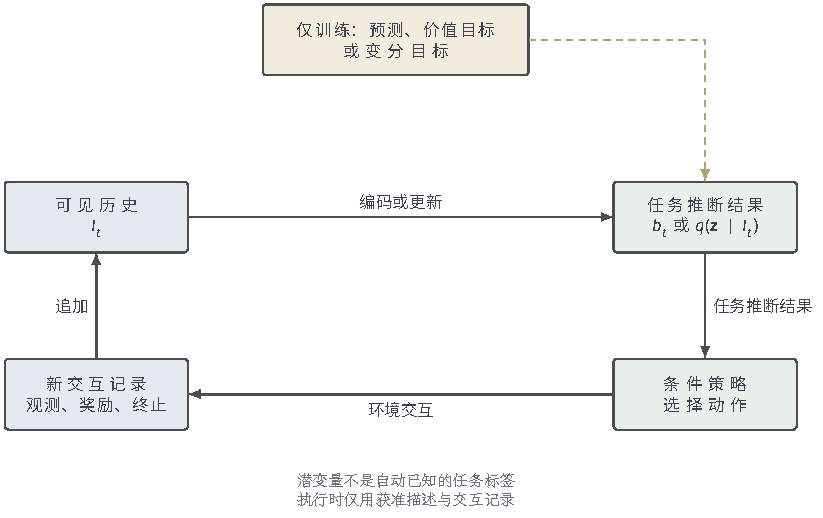
\includegraphics[width=139.446mm]{figures/10-reinforcement-learning/03-task-expansion-and-trustworthiness/tikz/rl-transfer-belief-loop.pdf}
 \caption{任务推断结果与行为的闭环。实线为执行时实际传递的观测、任务估计与动作，虚线为训练时用于塑造推断器的目标；传给策略的任务推断结果可以是精确后验、近似分布或普通历史编码，三者不能仅因向量维数相同就互换。图为本章机制的原创归纳。}
 \label{fig:rl-transfer-belief-loop}
\end{figure*}

\term{概率上下文元强化学习方法}（PEARL）把已收集的转移作为上下文$\mathcal C_t$，由编码器参数$\bm\varphi$形成潜变量$\bm z$的近似分布$q_{\bm\varphi}(\bm z\mid\mathcal C_t)$。从这个分布抽取$\bm z$后，策略据此选择动作，评论家据此评价动作。其原始设计把每条转移对应的高斯因子相乘并归一化，适合任务固定、转移可按集合处理的情形；离策略回放用于训练评论家与策略，编码器通过价值学习信号提取任务线索，相对先验的KL正则则约束潜变量分布。训练依次抽取任务、该任务上下文与回放转移，更新相应损失；部署收集获准的少量转移，更新潜变量分布，再抽样形成行为。这里保存的是任务潜变量的近似条件分布，不是已知真实风标签\scite{rl6-rakelly2019-pearl}

同样需要从历史提取任务线索，\term{变分贝叶斯自适应深度强化学习方法}（VariBAD）选择按时间递归编码历史，并通过变分目标学习潜变量。训练中的解码器用潜变量重建同一任务的奖励和转移，预测损失要求编码器保留能预测所记录奖励与后继观测的历史差别；KL项约束近似后验与先验或先前后验的差异。条件策略读取后验参数，而不只读取一个任务点估计，并以跨回合回报学习何时试探以取得新反馈、何时按现有后验选择高回报动作。执行时不需要调用训练用解码器做模型内规划。因此，训练中有预测解码器，并不能推出部署时采用基于模型的规划\scite{rl6-zintgraf2020-varibad}

回到右偏例子，现在要检验的是近似推断能否支持决策，而不是再演算一次贝叶斯公式。精确二任务模型给出$0.8$这一可核后验；近似编码器则需检查同类历史下的反馈预测与校准，不能要求某个潜变量坐标也恰好等于$0.8$。PEARL式抽样让行为在一个抽取的任务假设下连贯执行，VariBAD式条件策略可以依据分布的不确定性决定是否再探测；是否学到有效探索，仍依赖训练任务与反馈。前者要计算上下文因子及条件策略，后者要逐步维护循环状态和后验参数；两者训练还包含评论家或解码器成本，不能只比较策略前向次数。

存在比近似误差更根本的限制。构造两个终点隐藏的教学任务：在最后一次岔路选择前，预算内所有获准动作的状态、奖励和终止分布完全相同；最终向左或向右分别只在其中一个任务成功，先验各为$1/2$。任何历史编码器可读取的交互记录具有相同分布，因此最终选择左的概率在两任务中相同。若该概率为$p$，平均成功率为$\tfrac12p+\tfrac12(1-p)=1/2$。增加网络容量不能提高这项上限。只有允许额外访问会显示终点线索的状态，或提供带区分力的描述，主动辨识才可能改变预算内能够取得的任务线索。

% Outline: 6.5.2
\subsection{无目标任务更新数据下的零样本策略}
\label{sec:rl-transfer-zero-shot}

目标坐标已给出、状态编码和目标描述语义与训练一致时，策略形成可以只是一次条件查询：
$a_t\sim\pi_{\bm\theta}(\cdot\mid s_t,g)$，或
$a_t\in\argmax_a Q_{\bm\theta}(s_t,a,g)$。若同时给出可解释的新奖励权重，还可计算
\[
 a_t\in\argmax_a\max_i
 \langle\widehat{\bm\psi}^{\pi_i}(s_t,a),\bm w_g\rangle.
\]
后一种调用先用新权重给每项候选策略的后果计分，再对每个动作取策略库中的最高估值，最后选取估值最高的动作。它复用了SF策略库，不需要目标奖励样本；但共同动力学、终止与特征语义，以及第~\ref{thm:rl-transfer-gpi}~定理的估计条件仍不能省略。

这里沿用第~\ref{sec:rl-transfer-budget}~节的零样本口径：禁止用目标反馈更新权重、任务记忆或选择检查点，无论更新发生在回合内还是跨回合。当前观测仍然可见，否则连位置控制都无法执行；预先约定的物理状态滤波与未知任务辨识应分开报告。若把偏移或奖励反馈送入历史编码器，据此推断风向并改变后续控制，就已发生任务适应，即使尚未结束第一个回合、也没有一次反向传播。

可以在同一训练模型上固定目标坐标格式、动作选择规则和推理次数，分别测试图~\ref{fig:rl-transfer-task-plane}~中的$(1,0.15)$、$(3,0.3)$和$(4,0.45)$任务。它们依次代表支持内新任务、未见因素组合和范围外因素；训练参数与测试权限完全相同，变化的是所检验的任务关系。应分别报告三组零样本回报，而不是把它们合成一个“新任务平均分”。

若输入只有新编号3，条件网络无法由数字推断它代表哪个终点。若新目标需要从未形成的控制方式，或目标设备交换了左右动作接口，旧策略库即使每条策略都能前向计算，也可能没有一个合法有效的候选。零样本能力来自已有知识与描述之间成立的关系，不来自关闭更新开关本身。

% Outline: 6.5.3
\subsection{参数固定条件下基于上下文的策略适应}
\label{sec:rl-transfer-context-adaptation}

设想同一个隐藏风向的任务连续运行两个回合：第一回合先试探一下风往哪边吹，第二回合就根据观察到的偏移去绕开障碍。这已经是一种“适应”——行为根据新任务的反馈发生了改变。问题是：能不能在完全不改网络权重的前提下做到这一点？答案是可以，前提是策略必须把前一回合的证据保留下来，而不是每一步只看当前位置。此时真正变化的不是参数，而是历史记忆以及由它形成的任务估计。一个循环网络若在训练中见过足够多不同风向的任务，就可能把“如何利用历史推断任务并据此行动”这一学习过程本身，写进它的内部状态里。

\term{循环元强化学习方法}（RL$^2$）以循环策略把快速学习过程放入内部状态\scite{rl6-duan2016-rl2}
执行时固定网络参数$\bm\theta$，令
\begin{align}
 \bm m_t
 &=f_{\bm\theta}(\bm m_{t-1},o_t,a_{t-1},r_{t-1},\delta_{t-1}),\notag\\
 a_t&\sim\pi_{\bm\theta}(\cdot\mid\bm m_t).
 \label{eq:rl-transfer-rl2}
\end{align}
首步的上一动作、奖励与终止标记使用约定的空值。终止标记说明上一动作结束了物理回合；环境此时重置位置，但同一任务的$\bm m$继续保留。只有切换任务、开始新的独立适应试验时，才重置任务记忆。训练时在多项任务上优化跨多个回合的总回报，参数更新发生在这个较慢的过程里。目标覆盖同一任务的多个回合，早期探测的成本才可能由后续回合的收益补偿。

图~\ref{fig:rl-transfer-rl2-memory}~把固定参数外框与可变记忆分开。在前述教学风任务中，可构造一个实现贝叶斯更新的记忆器：初始记忆存右风概率$1/2$，第一个回合观察右偏后存$0.8$，第二回合用新概率选择路线。这个例子证明固定参数可以实现适应，不声称训练出的RL$^2$必然等价于精确贝叶斯推断。

\begin{figure*}[htbp]
 \centering
 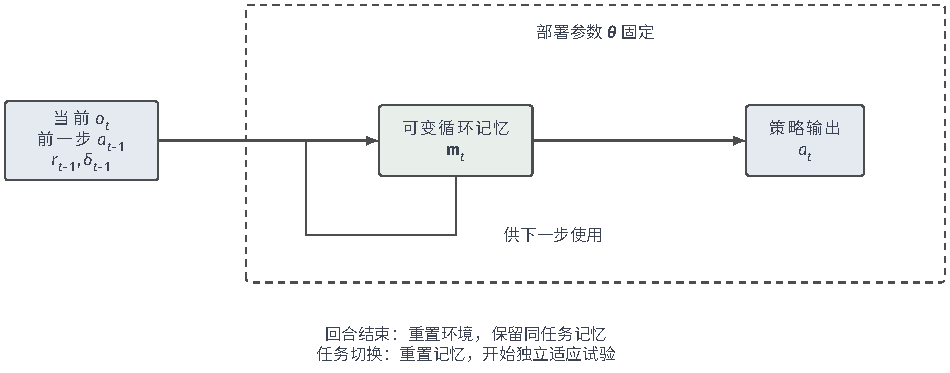
\includegraphics[width=160.800mm]{figures/10-reinforcement-learning/03-task-expansion-and-trustworthiness/tikz/rl-transfer-rl2-memory.pdf}
 \caption{固定参数中的可变记忆。输入包含当前观测及上一动作对应的奖励和终止标记；同任务回合结束仅重置物理环境，任务改变才重置记忆。图据RL$^2$的交互协议重绘，贝叶斯数值例是本章构造，不是其训练结果。}
 \label{fig:rl-transfer-rl2-memory}
\end{figure*}

若希望模型从已有算法的学习记录中学会怎样改进行为，可以保留记录中的回合顺序，而不只收集算法最终的动作。\term{算法蒸馏}（algorithm distillation, AD）据此从源强化学习算法的多回合学习记录抽取长序列，以自回归动作预测拟合
$-\sum_t\log\pi_{\bm\theta}(a_t\mid I_t)$\scite{rl6-laskin2023-ad}
输入历史包括观测、动作与奖励，训练样本保留从探索到改进的顺序；部署时把自身新经历追加到历史，固定参数继续预测动作。它模仿的是学习过程中的行为变化，而前述策略蒸馏通常只压缩已训练教师的行为。

AD的标签来自学习过程，未必是任务最优动作。\term{决策预训练Transformer}（decision pre-trained Transformer, DPT）改用任务内上下文和查询状态，预测教师给出的最优动作。训练时从任务$c$抽取上下文$D_c$和查询$s$，拟合
$-\log\pi_{\bm\theta}(a_c^*(s)\mid s,D_c)$；连续动作可使用相应密度损失。理想化地，若标签确为各任务最优动作、任务分布与上下文生成方式正确覆盖测试情形，监督条件分布会对仍与上下文相容的任务作后验混合。这解释了与后验采样的联系，不是任意有限网络都具备贝叶斯最优探索的保证\scite{rl6-lee2023-dpt}

\Needspace{26\baselineskip}
如果没有最优动作标签，也可以直接用交互回报训练记忆条件策略。\term{自适应智能体}（adaptive agent, AdA）在程序化任务空间中安排逐步调整的训练课程，训练带记忆的智能体，使跨回合反馈影响行为；其训练信号是交互回报，而非给定最优动作标签\scite{rl6-bauer2023-ada}

上下文还可以先用于评价动作，再用于形成策略。\term{可扩展上下文Q学习}（scalable in-context Q-learning, S-ICQL）利用世界模型生成任务提示，训练读取上下文的动作价值$Q$与状态价值$V$。它结合偏向高价值样本的expectile目标和优势加权策略提取。前者先拟合一个偏重高价值样本的状态价值，后者再用估计优势给策略训练样本赋权；两者解决的是不同步骤。测试上下文可以来自协议规定的在线交互或离线记录。

expectile中的“不对称”可以直接从残差看出。令待拟合状态价值为$v$，残差为$u=Q-v$；当$u>0$时，当前$v$低估了该动作价值。取$\omega\in(1/2,1)$，对正残差使用权重$\omega$，对负残差使用权重$1-\omega$，便会更重地惩罚这种低估。一个教学例有两个等权价值样本0和2，取$\omega=0.75$。在$v\in[0,2]$内，目标为
\[
  \frac12\left[0.25v^2+0.75(2-v)^2\right],
\]
导数为$v-1.5$，最小点为1.5。它高于样本均值1，却低于最大样本2，也不等于这两个样本的75\%分位数2。因而expectile是通过不对称平方惩罚改变拟合位置，并没有把最大样本直接认定为真实最优值。随后用$Q-V$构造估计优势并提高相应动作的策略拟合权重，是另一项操作。

Vintix II进一步考察DPT式决策预训练怎样使用多领域、含噪行为记录。它用这些记录构造上下文，再以示范者动作重标记监督目标，区分上下文中实际发生的行为与希望预测的动作。它的动作头不是一次回归出最终动作，而是学习怎样把噪声逐步变成动作。下面用$u\in[0,1]$表示动作生成过程的时间；$u$不是环境交互时刻$t$。

训练时，先由上下文与查询得到Transformer隐向量$\bm z_j^{\mathrm{hid}}$，再由高斯噪声$\bm x_0$和示范动作$\bm a^\star$构造线性路径
\[
  \bm x_u=(1-u)\bm x_0+u\bm a^\star.
\]
这条路径关于$u$的速度为$\bm a^\star-\bm x_0$。动作头以$\bm x_u,u,\bm z_j^{\mathrm{hid}}$为条件预测速度向量场，并用平方误差使预测速度接近这个标签。监督量因此是生成过程中的运动方向，而非把每个中间点直接回归为最终动作。

\begin{samepage}
执行时重新采样$\bm x_0$，沿学得的速度场数值积分，从$u=0$推进到$u=1$，把终点$\bm x_1$作为当前环境时刻的连续动作。用一维教学例可以区分训练与生成：噪声起点为0、示范动作为2时，路径为$x_u=2u$，训练速度标签为2。若学得的速度处处等于2，用Euler法手算两步、每步长度$0.5$，便依次得到0、1、2。真实动作分布中的速度场还依赖当前位置与上下文；这个例子只说明为何训练预测速度、执行却要积分生成动作。该方法同时研究在线与离线的上下文使用，其跨领域结果仍受所用低维观测、控制接口和训练任务支持约束，不能改写成任意视觉任务的通用保证\scite{rl1-polubarov2026-vintix}
\par
\end{samepage}

表~\ref{tab:rl-transfer-context-methods}~按上下文记录与策略形成方式对照这些方法。它们都能在固定参数下利用新上下文，但训练信号分别来自交互回报、学习历史中的动作、教师标签或条件价值估计。这些差别决定了模型能够从训练任务的交互记录及动作标签中学到什么，不能仅以是否使用Transformer判断适应机制。

\begin{table*}[t]
 \centering\small
 \begin{tabularx}{\linewidth}{@{}>{\raggedright\arraybackslash}p{20mm}*{4}{>{\raggedright\arraybackslash}X}@{}}
  \toprule
  方法 & 上下文内容 & 训练样本来源 & 目标反馈 & 策略提取\\
  \midrule
  RL$^2$ & 观测、前动作、奖励、终止 & 多任务在线跨回合交互 & 同任务内逐步到达 & 循环记忆条件策略\\
  AD & 按顺序的多回合学习历史 & 源RL算法的学习轨迹 & 追加自身交互历史 & 自回归预测动作\\
  DPT & 任务内转移及查询状态 & 上下文与教师最优动作标签 & 给定上下文或新交互 & 监督条件动作分布\\
  AdA & 跨回合观测、动作与反馈 & 程序化任务、课程与在线RL & 试验内持续反馈 & 记忆条件的RL策略\\
  S-ICQL & 任务提示与交互上下文 & 世界模型提示和离线记录 & 在线或离线上下文 & 条件价值与优势加权策略\\
  Vintix II & 多领域转移上下文 & 含噪记录、示范者动作重标 & 在线或离线上下文 & DPT式条件化与流匹配动作头\\
  \bottomrule
 \end{tabularx}
 \caption{固定参数上下文适应的不同训练信号。各方法的上下文、反馈量和策略提取成本必须单独核对；该表归纳原始方法，不表示使用同一批训练样本得到的实验排名。}
 \label{tab:rl-transfer-context-methods}
\end{table*}

表中的差别并不只在网络输出形式。AD直接拟合学习历史中的动作，S-ICQL先学习条件价值，再按估计优势给策略训练样本加权。二者都可在固定参数下适应，但历史进入决策的训练依据不同\scite{rl1-liu2026-sicql}

这类方法的运行代价不止权重存储。循环策略每步更新固定维度记忆，长序列Transformer在朴素实现中对长度$L$的完整注意力计算为$O(L^2)$；缓存可以减少重复计算，但仍要存储上下文及相关状态。条件价值可能需要额外候选动作评价；Vintix II采用的流匹配动作头还需若干生成步骤\scite{rl1-polubarov2026-vintix}
比较时应报告实际上下文长度、缓存、推理次数与延迟，不把“零梯度步”写成“零适应成本”。

任务边界错误也会改变结果：把前一任务记忆带入下一任务会污染推断，过早清空记忆会丢掉跨回合证据；截断窗口可能删掉唯一的风向线索。学习轨迹若只有无效随机行为，AD无法仅靠动作模仿获得未出现的改进规则；教师标签、世界模型和任务生成器也各有支持限制。训练中学到某种改进模式，并不意味着在任意新任务上都能保证探索和性能单调提升。

% Outline: 6.5.4
\subsection{允许有限梯度更新下的参数适应}
\label{sec:rl-transfer-gradient-adaptation}

前一小节把风向证据写进了记忆、参数始终不动。如果协议还允许修改参数，就多了一条路：把获准取得的目标任务交互记录当作适应训练样本，直接调整策略本身，这就是基于梯度的快速适应。它要估计的是“当前策略参数对目标任务回报的梯度”，而不是去预测任务编号或给风向做分类。其背后的思路常被称为“学会学习”（元学习）：在训练阶段，不只是让策略在各任务上表现好，而是让它的初始参数处在一个“只需在新任务上走几步梯度就能变好”的位置。设任务$c$在适应期间固定，从$\bm\theta^{(0)}=\bm\theta$出发，以当前策略收集$D_c^{(0)}$。对于有限时域折扣回报，令
$L_c(\bm\theta)=-\mathbb E[\sum_{t=0}^{H-1}\gamma^t r_t]$；
终端价值取0。沿用策略梯度的可微性、环境不依赖策略参数及可积性条件，可构造
\begin{align}
 \widehat{\bm g}_c
 &=-\frac1N\sum_{j=1}^N\sum_{t=0}^{H-1}
   \gamma^t\nabla_{\bm\theta}\log\pi_{\bm\theta}
        (a_{j,t}\mid I_{j,t})
   \bigl(G_{j,t}-b(I_{j,t})\bigr),\notag\\
 \bm\theta'&=\bm\theta-\alpha\widehat{\bm g}_c.
 \label{eq:rl-transfer-inner-update}
\end{align}
$N$是独立采集的轨迹数，$G_{j,t}$是轨迹$j$从动作时刻$t$起的折扣回报。把动作的对数概率梯度乘以回报，再对轨迹平均，估计提高高回报动作概率的方向；基线$b$用于减少方差，不能依赖当前所采动作，且在此梯度中视为固定。式中额外的$\gamma^t$来自起点目标的折扣；损失是负回报，所以减去负回报梯度才对应提高回报。该样本梯度可记作
$\nabla_{\bm\theta}\widehat L_c$，但不能通过把环境奖励当成参数的普通可微函数来获得它。

\begin{example}[一次目标任务参数更新]
 \label{ex:rl-transfer-gradient-step}
 将导航末端岔路简化为独立单步教学任务：向右奖励1、向左奖励0，动作概率为
 $p_\theta=\pi_\theta(\text{右})=\sigma(\theta)$，初值$\theta=0$，基线0。收集4次独立试验，假设实际抽到3次右、1次左。对于右动作，
 $\partial_\theta\log p_\theta=1-p_\theta=1/2$；左动作奖励0，贡献为0。于是
 \[
 \begin{aligned}
 \widehat g&=-\frac{3(1/2)}4=-\frac38,\qquad
 \alpha=2,\qquad \theta'=\frac34,\\
 p_{\theta'}&=\frac1{1+e^{-3/4}}\approx0.6792.
 \end{aligned}
 \]
 更新前的真实期望回报为$0.5$，更新后为$0.6792$。这里能够直接算真实值，是因为教学任务的奖励模型已完整给出；实际未知任务需要另采独立评价回合来估计回报。4条记录的经验回报$0.75$既不是更新前真实值，也不能作为更新后性能证明。
\end{example}

执行顺序因此是收集、估计、更新、另行评价。扩展为$K$步时，用
$\bm\theta^{(k+1)}=\bm\theta^{(k)}-\alpha_k\widehat{\bm g}_c^{(k)}$；
每步若按同策略估计，需要由更新后策略新采的轨迹训练样本，复用旧策略的轨迹记录则必须采用适当离策略估计并满足覆盖条件。固定日志不提供未记录动作的反事实回报，允许梯度计算也不会自动补齐这一缺口。

第~\ref{sec:rl-transfer-value-training}~节的MAML外循环还需评价更新对初始化的依赖。保留
$\bm I-\alpha\nabla^2\widehat L_c$是在给定内层样本时反传内循环导数；一阶近似以$\bm I$代替这一Jacobian，减少高阶自动微分开销。二者都还需交代整批训练样本律$Q_{c,n}^{\pi_{\bm\theta}}$的采样分布项是否纳入估计；示例~\ref{ex:rl-transfer-sampling-gradient}~说明，即使固定记录的导数为0，完整期望梯度也可能非零。部署时执行若干普通目标梯度步，本身并不需要再计算元梯度。

表~\ref{tab:rl-transfer-storage}~按新任务记录或估计结果写入的位置比较适应机制。计算成本包括训练所需的反向传播、优化器状态和独立评价，而不只是最终策略推理。

\begin{table*}[t]
 \centering\small
 \begin{tabularx}{\linewidth}{@{}>{\raggedright\arraybackslash}p{19mm}*{4}{>{\raggedright\arraybackslash}X}@{}}
  \toprule
  机制 & 记录或估计的存储位置 & 变化内容 & 重置与可逆性 & 主要代价\\
  \midrule
  上下文适应 & 历史窗口、循环状态 & 新经验与压缩记忆 & 可清空；被截断的历史记录未必可恢复 & 记忆存储、序列前向\\
  任务信念 & 离散概率或后验参数 & 各假设的相对可信度 & 可重置先验；恢复旧后验需保存证据或快照 & 似然、归一化或近似推断\\
  参数适应 & 策略、价值或模型权重 & 梯度及优化器状态 & 有初值快照才可完整回滚 & 前后向、优化器、再评价\\
  \bottomrule
 \end{tabularx}
 \caption{目标任务记录与估计结果的存储位置。这是机制比较而不是互斥分类：后验可作为上下文输入，记忆更新也可与参数更新同时执行。}
 \label{tab:rl-transfer-storage}
\end{table*}

少量样本估计的梯度可能有较大波动，过大步长可能破坏原有行为；模型错配或离策略权重过大还可能使估计方向失真。教学例中的一次改进不能推成一般单调保证。没有获准用于更新的目标任务训练样本、只获准固定参数部署，或探测动作违反可行动作约束时，就不能默认运行这套流程。

% Outline: 6.5.5
\subsection{持续交互下的任务辨识与在线适应}
\label{sec:rl-transfer-identification}

如果未知风向在整个部署期间都固定不变，那么早先收集到的有效观测始终在指向同一个当前任务，持续交互就能让判断越来越准。但这里有一个容易被忽视的陷阱：一个只沿安全边界走、从不经过受风影响位置的策略，可能拿到稳定的回报，却永远辨认不出风向。也就是说，持续交互要想真正减少不确定性，所选的行为必须能带来区分性的证据；而是否值得为此专门去“试探”，还要权衡探测本身的成本与弄清任务后能带来的控制收益——这正是第\ref{chap:rl-learning}章探索与利用张力在任务层面的再现。

把这一取舍简化为独立的两阶段、不折扣教学任务。两种风先验各半；终端安全路线奖励$0.6$，按正确风向选择的捷径奖励1、选错奖励0。直接选择时，捷径期望$0.5$，故安全路线较好。若第一阶段允许付出$0.1$奖励成本，执行一个正确率$0.8$的对称风向探测，再按信号选择捷径，则总期望回报为$-0.1+0.8=0.7$。不探测的策略在第一阶段等待且不扣分，两者使用相同两阶段时域。探测提高了终端决策的期望回报$0.2$，付出成本$0.1$，净收益$0.1$；若探测成本改为$0.3$，原方案就不再值得。

同一个正确率$0.8$的探测，在两种成本下得到不同决策，所以探测反馈的收益必须由它带来的后续回报改变量评价，不能只看任务分类准确率。在线过程可以每收集一小批转移便更新一次后验和策略，也可以逐步更新记忆、偶尔更新参数。当前任务估计影响行为，行为改变后续观测、奖励与终止记录的分布，新记录再更新任务估计或控制规则。只更新后验、只更新参数或同时更新两者，都可能形成这样的闭环，但代价和稳定性不同。

图~\ref{fig:rl-transfer-identification-curves}~刻意把任务辨识误差和控制回报画在两个坐标系中。早期两条曲线同时表现为辨识误差较大、控制回报较低，这一并存现象只提示应检查任务辨识误差是否限制控制；仅凭两条独立设定的解析曲线，不能确定低回报的原因。后来误差已经很低而回报仍未达到目标，则提示还需检查规划或控制。图中的解析曲线只描述一种待检验的诊断情形，不是任何方法的收敛率，也没有假设分类误差可以直接换算成回报。

\begin{figure}[htbp]
 \centering
 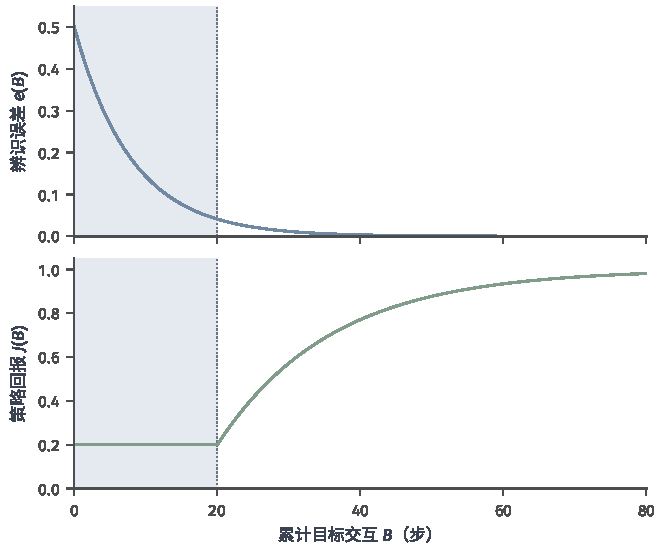
\includegraphics[width=112.000mm]{figures/10-reinforcement-learning/03-task-expansion-and-trustworthiness/matplotlib/rl-transfer-identification-curves.pdf}
 \caption{固定任务下辨识与控制的不同进度。教学解析曲线为$e(B)=0.5e^{-B/8}$和$J(B)=0.2+0.8(1-e^{-\max(B-20,0)/16})$；$B$为累计目标交互步数。竖线$B=20$用于分区说明，非实测拐点，亦非理论阈值。两图共享横轴，不共享纵轴量纲。}
 \label{fig:rl-transfer-identification-curves}
\end{figure}

误差可以按已知测试标签计算，也可以按后验对真实任务的概率或参数偏差计算，报告时需固定一种定义。部署系统没有真实任务标签时，只能用已观测反馈检查预测残差、反馈预测的校准或其他可观察证据；检验任务后验本身的校准仍需真实任务标签，不能把测试者知道的风向反送给策略。实际测量还应改变探测预算，分别检查任务辨识误差是否降低，以及固定同一组任务描述与记录后控制回报是否提高。

探测、回到测试位置、失败恢复和再评价全部消耗资源。更多交互只有在可识别、能到达相关状态且反馈权限充分时才有帮助。若辨识需要越过禁止区域，不能以“学习所必需”为理由默认开放动作；安全探索与约束可行性见第~\ref{chap:rl-trustworthy}~章。

% Outline: 6.5.6
\subsection{任务持续变化下的跟踪与适应}
\label{sec:rl-transfer-tracking}

现在把固定风向改成回合间突变，或让风强度缓慢漂移。上个回合的右偏仍是真实记录，却可能不再代表当前风向。直接把式~\eqref{eq:rl-transfer-belief-update}~用于全部历史，会把已失效的证据累积成过度自信；要继续作贝叶斯推断，需要额外给出任务变化模型，否则应采用明确的跟踪估计。

处理过时证据有几种不同办法。变化检测与重启先检查预测残差是否异常，再丢弃或下调旧模型；滑动窗口只保留最近$W$条记录；历史降权则给年龄为$j$的样本权重$\lambda^j$，其中$0<\lambda<1$。它们分别决定何时停用旧估计、保留多少近期交互记录，以及旧记录随时间减轻多少影响。窗口大或$\lambda$接近1时，稳定阶段估计方差较低，变化后的响应却较慢。例如独立Bernoulli观测在固定参数下，窗口均值的方差为$\eta(1-\eta)/W$；参数突变后，这个均值在旧记录移出前仍混合两种机制。检测阈值还要在误报、漏报和延迟间取舍。

检测出风向变化以后，重新估计和恢复控制仍会损失回报。要累计评价这段代价，需要先规定每次变化后的比较对象。考虑共同有限状态动作空间、共同初始分布$\mu_0$的回合式任务序列，各回合逐步奖励有界。第$k$回合的MDP为$\mathcal M_k$，在该回合内固定，时域为$H$；用不折扣总奖励
$V_{k,0}^{\pi}(\mu_0)=\mathbb E_{\mu_0,\pi,\mathcal M_k}
[\sum_{t=0}^{H-1}r_{k,t}]$，终端价值0。$r_{k,t}$仍按回合内动作时刻编号，与无限折扣目标分别使用。令$\pi_k$是算法基于此前观测、动作与奖励记录选择的本回合行为规则，可以在回合内依靠新历史行动。

\begin{definition}[动态遗憾与静态遗憾]
 \label{def:rl-transfer-regret}
 给定正整数$T,H$及$T$个回合任务，各回合从共同初始分布$\mu_0$启动，采用前述相同的$H$步不折扣总奖励与行动前历史权限。记$V_{k,0}^{\pi}(\mu_0)$为策略$\pi$在第$k$个任务中的期望回报，要求所比较的回报有限；$V_{k,0}^*(\mu_0)$是知道该回合任务模型、仍只按获准历史行动的策略类中的有限最优值。动态遗憾逐回合计算算法策略$\pi_k$比这一最优值少多少，再相加：
 \begin{equation}
 \operatorname{DReg}_T
 =\sum_{k=0}^{T-1}\left[
 V_{k,0}^{*}(\mu_0)-V_{k,0}^{\pi_k}(\mu_0)\right].
 \label{eq:rl-transfer-dynamic-regret}
 \end{equation}
 若比较者必须始终使用同一策略，就在预定的非空固定策略类$\Pi_{\text{固定}}$中，取整段序列累计回报的上确界；假设该上确界有限。相对于这一比较值的静态遗憾为
 \begin{equation}
 \operatorname{SReg}_T
 =\sup_{\pi\in\Pi_{\text{固定}}}
       \sum_{k=0}^{T-1}V_{k,0}^{\pi}(\mu_0)
       -\sum_{k=0}^{T-1}V_{k,0}^{\pi_k}(\mu_0).
 \label{eq:rl-transfer-static-regret}
 \end{equation}
 固定比较策略不随回合改变，可依赖回合内时间与允许观测；不能暗含当回合隐藏任务标签。若另有条件保证最优比较策略存在，上确界可以写成最大值。随机任务序列或随机算法下，另对这些随机性取期望。
\end{definition}

动态比较者在每次变化后都立即知道新的奖励与转移，显著强于部署者。静态比较者只选一个共同规则；算法若成功跟踪变化，甚至可能优于它，故静态遗憾不应解释为适应延迟。两者必须使用相同初始分布；如果还改变初始分布，应把它列入变化机制和评价条件。

动态比较者每回合都能换成当前最优策略，而部署者需要从反馈认识变化。若要使平均每回合差额随回合数增长而趋于0，即取得次线性动态遗憾，就需要约束环境变化或另给关于当前任务参数的提示。例如可限制相邻回合任务改变的次数
$S_T=\sum_{k=1}^{T-1}\mathbb I\{\mathcal M_k\ne\mathcal M_{k-1}\}$，
或者在共同有界奖励尺度下定义
\begin{align}
 B_R&=\sum_{k=1}^{T-1}\sup_{s,a}|R_k(s,a)-R_{k-1}(s,a)|,\notag\\
 B_T&=\sum_{k=1}^{T-1}\sup_{s,a}
 \lVert T_k(\cdot\mid s,a)-T_{k-1}(\cdot\mid s,a)\rVert_1.
 \label{eq:rl-transfer-variation}
\end{align}
每项上确界取相邻回合在所有状态动作上的最大变化，$B_R$累加奖励均值的变化幅度，$B_T$累加转移分布的$L^1$变化幅度。使用全部状态动作，而不只使用当前策略产生的交互记录，是为了限制环境本身的变化；未访问位置的变化也可能影响后续最优决策。变化次数、累计幅度与单次最小可检测幅度不是同一个量。频繁微小漂移可以次数多而累计幅度小；一次大跳变也可能因相关状态不可达而难以检测。是否给出变化提示、提示是否含新任务参数，以及是否已知变化预算，都需单独说明。非平稳学习理论是在这些条件下研究性能，而非取消所有条件后承诺及时适应\scite{rl6-wei2021-nonstationary}

\begin{theorem}[无预告快速变化的两臂下界]
 \label{thm:rl-transfer-linear-regret}
 在$H=1$的教学任务族中，每轮$k$独立均匀抽取
 $C_k\in\{1,2\}$，动作集合为两个臂，奖励为
 $r_k(a)=\mathbb I\{a=C_k\}$。选择动作前不给任何关于$C_k$的线索；选择后可以观察所得奖励。对任何使用过去历史、内部随机源与任务序列独立的随机算法，以知道当轮$C_k$并选择相应臂的策略作动态比较者，有
 \[
 \mathbb E[\operatorname{DReg}_T]=T/2.
 \]
\end{theorem}

\begin{proof}
 令$\mathcal F_k$包含第$k$轮之前的全部动作、奖励及算法已用的随机数。算法还可使用与任务序列独立的新随机数$U_k$，据
 $(\mathcal F_k,U_k)$选择$A_k$。由构造，$C_k$与上述$\mathcal F_k$和本轮新随机数$U_k$独立，且在两臂上均匀分布，因此不论条件动作概率如何，
 对条件概率为正的动作$a$，
 $\mathbb P(C_k=a\mid\mathcal F_k,U_k,A_k=a)=1/2$。
 对动作分支求和便得
 \begin{align*}
 \mathbb P(A_k=C_k\mid\mathcal F_k,U_k)
 &=\sum_{a=1}^2
    \mathbb P(A_k=a\mid\mathcal F_k,U_k)\,\tfrac12\\
 &=\tfrac12.
 \end{align*}
 取全期望，每轮算法的期望奖励为$1/2$。知道当前任务$C_k$的动态比较者选择臂$C_k$，每轮奖励恒为1；它不需要预知任何未来任务。由期望的线性性，
 \[
 \mathbb E[\operatorname{DReg}_T]
 =\sum_{k=0}^{T-1}\left(1-\mathbb E[r_k(A_k)]\right)
 =\sum_{k=0}^{T-1}(1-\tfrac12)=T/2.
 \]
 轮末反馈即使揭示了本轮完整任务，也不能预测独立的下一轮，所以结论不依赖算法的记忆容量、计算时间或参数更新能力。
\end{proof}

这一下界不否认缓慢变化可以跟踪，也不否认预告信号可以帮助决策。它只指出：比较者知道当前最好动作而算法在选择前毫无线索时，无规律快速变化本身足以产生线性代价。静态比较者的期望优势却小得多。令$N_1$为$T$轮中臂1高奖励的次数，最佳固定臂奖励为
$T/2+|N_1-T/2|$；由方差及Cauchy--Schwarz不等式，
$\mathbb E|N_1-T/2|\leq\sqrt{T}/2$。因此同一算法对固定臂的期望静态遗憾至多$\sqrt{T}/2$，而动态遗憾仍是$T/2$。换比较对象就换了结论。

图~\ref{fig:rl-transfer-tracking}~进一步区分变化发生、变化检测和性能恢复三个时刻。检测准确也不等于立即恢复：模型重估、规划与控制学习仍有代价。恢复阈值和观察窗口应提前规定，不能看到曲线后再选最有利时刻。

\begin{figure}[htbp]
 \centering
 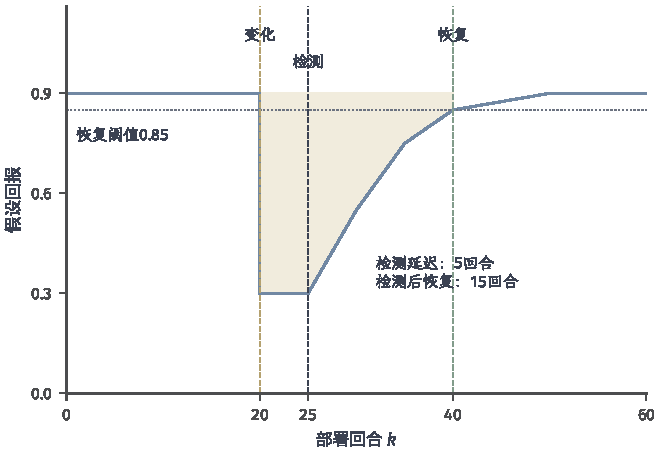
\includegraphics[width=112.000mm]{figures/10-reinforcement-learning/03-task-expansion-and-trustworthiness/matplotlib/rl-transfer-tracking.pdf}
 \caption{变化、检测与恢复的教学时间线。曲线由图源中给定的分段线性控制点生成；变化在回合20，检测在25，首次达到预设回报阈值$0.85$在40。下降、延迟和恢复期间的差额各有含义，非任何算法的实测轨迹。}
 \label{fig:rl-transfer-tracking}
\end{figure}

若系统从不按回合重置，前期动作会影响变化发生时的物理状态，就应使用适合持续过程的平均回报、动态比较规则或跟踪损失，不能原样套用共同$\mu_0$的式~\eqref{eq:rl-transfer-dynamic-regret}。变化期间的决策代价由动态比较规则或跟踪损失衡量；旧能力保留、遗忘和一般持续学习理论可参考\BookVolumeRef{vol:knowledge-learning}{卷8《学习范式：知识的获取、演进与迁移》}中的知识演进与知识迁移部分。

% Outline: 6.5.7
\subsection{任务信息与适应权限的组合边界}
\label{sec:rl-transfer-combinations}

目标坐标已知时，陌生地面仍可能要求估计摩擦参数；隐藏风向没有描述时，记忆中积累的偏移证据也可以改变条件策略，不必改网络权重。前面分别讨论的描述、记忆、梯度更新与持续交互，因此可以出现在同一系统中。描述决定已知哪些任务条件，其他机制决定怎样取得缺少的任务反馈并形成相应估计。

表~\ref{tab:rl-transfer-permissions}~以任务描述及反馈可见条件为行、机制权限为列。每格写的是该组合所需的证据和接口，而非给方法贴一个永久类别标签。

\begin{table*}[t]
 \centering\small
 \begin{tabularx}{\linewidth}{@{}>{\raggedright\arraybackslash}p{18mm}*{4}{>{\raggedright\arraybackslash}X}@{}}
  \toprule
  描述与反馈条件 & 零样本调用 & 上下文更新 & 参数更新 & 持续交互\\
  \midrule
  显式描述 & 描述语义、范围与接口兼容；不读目标反馈学习 & 描述加获准历史；反馈可补描述遗漏 & 描述加日志或新样本；允许反传 & 允许探测描述未给出的动力学；全部计费\\
  隐藏任务 & 依据先验、已给描述及正常控制所需观测选择；不据目标反馈辨识任务或选模 & 历史须含区分性反馈；规定窗口与重置 & 更新样本须支持估计；不使用隐藏标签 & 可达的区分动作、反馈权限与恢复预算\\
  \bottomrule
 \end{tabularx}
 \caption{任务描述、可见反馈与适应权限的组合。各列可同时启用，持续交互规定可采集哪些目标任务记录，不是与记忆或梯度互斥的网络结构。}
 \label{tab:rl-transfer-permissions}
\end{table*}

例如，显式目标加两步梯度更新可以用目标选择损失，再由新转移修正行动者；但两步所用交互、学习率选择和更新后评价仍须纳入预算。隐藏风向加固定参数记忆则可用第一回合判断风向、第二回合选路；它不消耗梯度步，却消耗反馈和上下文。两种组合只有在总交互次数、可读描述与反馈可比时，才有理由比较“适应更快”。

技能复用也遵循这一划分。任务描述或信念决定高层在合法启动集内选哪项技能，技能结束后根据新观测再组合下一项；若允许更新，可以只改高层选择器，也可以调整技能内部控制参数。后者可能改变持续时间与终止分布，应重新检查与高层价值估计的接口，而不能把内部更新当作无影响替换。技能定义与单任务时间抽象仍沿用第~\ref{chap:rl-learning}~章。

比较方法前应同时固定目标交互数、反馈字段、上下文容量、梯度步数及额外计算。主动辨识与基于测试成绩的选模都使用目标任务的交互反馈或测试成绩，不能从预算中删除。适应机制的组合越灵活，实验协议越需要明确。

% Outline: 6.6
\section{迁移结论的验证与修正}
\label{sec:rl-transfer-validation}

最后要问：怎样确认迁移真的发生了，以及它在什么范围内成立？一个模型在新终点上拿到较高回报，可能是真的直接调用了旧知识，也可能是在测试过程中已经偷偷读取了大量新任务的反馈；只报告一个平均成绩，还可能把强风任务上的失败淹没掉。因此，前面陆续给出的共享条件、任务描述与反馈、策略形成机制，都需要在验证环节逐项落实：测试任务从哪里来、反馈何时可见、预算如何累计、与谁作比较。只有把这些交代清楚，才能确定一个分数究竟支持的是哪一项迁移主张。

% Outline: 6.6.1
\subsection{由目标任务适用范围确定任务级数据划分}
\label{sec:rl-transfer-split}

同一风向、同一目标下的轨迹随机分成两组，只检验任务内的新经历。要回答换任务后能否复用，就应先在任务层划分：检验支持内新任务时，留出完整任务身份；检验组合泛化时，留出目标与噪声的指定组合；检验范围外能力时，把相应因素范围从训练和调参任务中排除。每一种划分都对应前面声明的一种目标任务关系。

图~\ref{fig:rl-transfer-split}~按任务、回合、片段三层展示这一差别。同一回合的相邻片段共享物理轨迹，同一任务的不同回合共享隐藏参数；把它们都视为独立任务会严重夸大证据量。

\begin{figure*}[htbp]
 \centering
 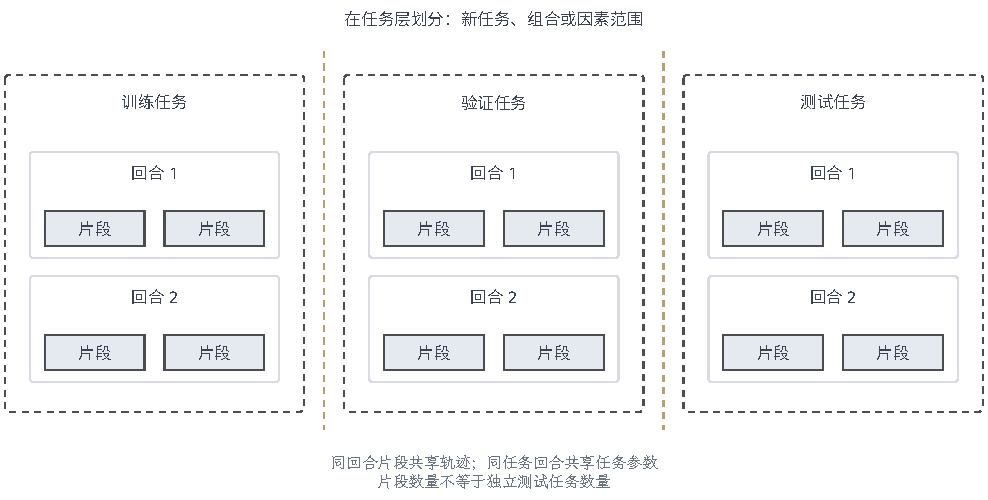
\includegraphics[width=167.238mm]{figures/10-reinforcement-learning/03-task-expansion-and-trustworthiness/tikz/rl-transfer-split.pdf}
 \caption{任务级划分与任务内采样。训练、验证、测试先按所声明的任务关系划分，再在每项任务内采集回合和片段；同色框中片段共享任务参数，不能按片段数声称独立任务数。图为抽样层级示意，不对应某批实际采集的任务或回合数量。}
 \label{fig:rl-transfer-split}
\end{figure*}

例如，三个独立生成的风向任务各采10回合，每回合切20段，共有600个片段，但任务层独立单位仍只有3个。这些是教学计数。若要评估任务平均回报的不确定性，应在任务层重采样，或用明确的分层统计模型；训练种子另是模型训练随机性的层级，不能将同一个训练种子下的600段当作600次独立训练。增加任务内完整回合主要改善已见任务中的回报估计，增加独立任务才增加关于任务总体的独立证据。一般的两层抽样界还要求固定完整学习或适应规则、在可见记录上定义有界评价损失，并核对任务独立、给定任务后的完整运行条件独立及候选选择方式；任意相邻RL片段不能直接满足这些条件。

测试协议应预先固定是否允许交互、奖励到达时刻、回合结束与任务切换的记忆重置，以及检查点数量。非平稳测试还要固定任务时间顺序；打乱时间后进行批量拟合，使用的是另一种历史读取与回合重排权限。不能让策略提前看到未来风向标签，也不能在恢复时间统计中删除失败回合。

泄漏不只来自重复轨迹。程序化生成器可能只更换纹理而复用同一路线模板，共享随机种子可能重现测试布局，目标描述可能直接包含最优动作编码。应检查生成器结构、种子谱系和描述字段。允许在一项测试任务内按既定协议适应，不等于允许根据整套测试成绩反复重设计训练方法；后一种选择应在验证任务上完成。

% Outline: 6.6.2
\subsection{在任务划分与固定预算下取得性能证据}
\label{sec:rl-transfer-evidence}

同一模型在新风向下先探测、再控制，探测期间的回报可能很低，适应完成后却能稳定到达终点。验证需要分别回答初始能做什么、学习期间付出多少代价、学完后能做什么。用$n$表示测试任务数，令$c_i$为第$i$个测试任务，$\pi_{i,0}$为尚未使用该任务的适应训练样本时的策略；$\pi_{i,B}$为按协议使用$B$步反馈后形成的策略。若使用前面的无限折扣任务，回报仍为未归一化$J_{c_i}$；若评价固定长度回合，则另注明时域、折扣和截断规则。

\term{零样本回报}为
$n^{-1}\sum_iJ_{c_i}(\pi_{i,0})$。\term{适应后回报}为
$n^{-1}\sum_iJ_{c_i}(\pi_{i,B})$，需要固定适应所得参数和任务后验或历史记忆、在独立评价回合上估计，并另报这部分交互数。评价时仍可按协议更新控制所需的物理状态估计，但不继续辨识任务；若一个记忆器无法分开这两项功能，就应明确评价中仍在适应。\term{预算内适应曲线}则记录随着累计目标交互增加，当前在线回合实际取得的回报，或在指定检查点另测的回报；这两种曲线不能混标，后者的查询成本也不能省略。

为评价学习期间的损失，固定同一目标任务、同一回合时域与初始分布，取指定比较策略$\pi_i^{\text{参照}}$。用$\pi_i^{(k)}$表示第$k$个适应回合的行为规则，区别于使用$B$步反馈后的$\pi_{i,B}$。在$M$个适应回合中定义
\begin{equation}
 \operatorname{AReg}_{i,M}
 =\sum_{k=0}^{M-1}
 \left[J_{c_i}(\pi_i^{\text{参照}})
       -J_{c_i}(\pi_i^{(k)})\right].
 \label{eq:rl-transfer-adaptation-regret}
\end{equation}
每个差额都以同一任务和回合条件下的参照回报为起点，求和得到学习期间相对该参照的累计损失。若比较者只是一条训练得到的策略，算法也可能超过它，使该量为负；名称不赋予参照者最优性，必须写出它可读取的任务标签、观测及模型字段。任务本身变化时，原来固定的$c_i$已不能代表所有回合，应另用式~\eqref{eq:rl-transfer-dynamic-regret}~及检测、恢复指标。

表~\ref{tab:rl-transfer-baselines}~给出比较协议。$B,K,L,C$分别表示目标适应步、梯度步、上下文长度和额外计算上限；它们是符号预算，不是某篇论文配置。共享训练的前期成本也应报告，即使目标任务比较只匹配部署预算。

\begin{table*}[t]
 \centering\small
 \begin{tabularx}{\linewidth}{@{}>{\raggedright\arraybackslash}p{23mm}*{3}{>{\raggedright\arraybackslash}X}@{}}
  \toprule
  比较对象 & 可用模型、任务描述与记录 & 目标预算 & 解释范围\\
  \midrule
  从头学习 & 随机初始化，不用源任务知识 & 相同$B,K,L,C$，独立评价另计 & 共享训练是否减少目标学习代价\\
  无适应 & 相同源模型，关闭任务更新 & 适应交互0、梯度0；执行预算相同 & 初始能力与适应带来的变化\\
  单任务训练 & 不共享参数的指定任务训练 & 报预训练量；目标比较仍匹配$B,K,L,C$ & 共享收益与容量、训练量差异\\
  已知任务身份 & 额外给真实任务参数 & 其余预算匹配，真实参数读取权限另标 & 知情参考；训练策略未必是上界\\
  可证明最优值 & 完整已知模型或允许额外读取真实状态或参数的可证明松弛 & 比较者权限显式列出 & 条件成立时才是性能上界\\
  \bottomrule
 \end{tabularx}
 \caption{性能证据需要的参照对象。“无适应”是刻意关闭反馈学习的消融，不能假装它花掉了与适应方法相同的学习预算；单任务参考若用目标任务交互记录预训练，必须披露这批额外目标任务训练样本。}
 \label{tab:rl-transfer-baselines}
\end{table*}

匹配预算以后，仍要区分平均水平与任务间差异。图~\ref{fig:rl-transfer-evaluation-curves}~用一组可复算的教学曲线说明汇总方法：设目标任务$i=1,\ldots,5$、训练种子$j=1,\ldots,3$，定义假设回报
\[
 \begin{aligned}
 y_{i,j}(B)&=0.2+0.7(1-e^{-B/30})+u_i e^{-B/60}+v_j,\\
 u_i&\in\{-0.16,-0.08,0,0.08,0.16\},\\
 v_j&\in\{-0.02,0,0.02\}.
 \end{aligned}
\]
式中共同项随预算$B$增加，$u_i$给出随适应减小的任务偏差，$v_j$给出训练种子偏差。所有数值都是作者设定的回报尺度，每条曲线是给定公式，不是实验测量。任务与种子均等权时，先对种子平均，再对任务平均；两组偏差分别和为0，得到均值$m(B)=0.2+0.7(1-e^{-B/30})$。阴影取种子平均后任务分数的均值加减一个样本标准差，即
$s_{\text{任务}}(B)=\sqrt{0.016}\,e^{-B/60}$，不是均值的置信区间。实际实验还需估计评价回合随机性，并说明任务与训练种子的嵌套或交叉方式。

\begin{figure}[htbp]
 \centering
 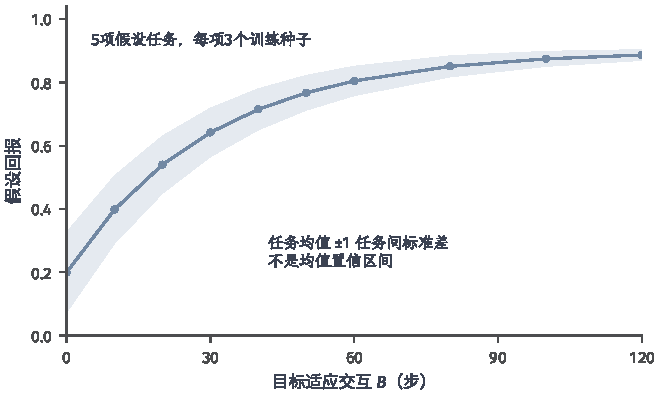
\includegraphics[width=112.000mm]{figures/10-reinforcement-learning/03-task-expansion-and-trustworthiness/matplotlib/rl-transfer-evaluation-curves.pdf}
 \caption{固定预算下均值与任务间离散程度的教学曲线。横轴为目标适应交互步数，纵轴为假设回报；线为5任务、3训练种子的等权均值，阴影为先平均种子后的任务均值$\pm1$样本标准差。图源按正文公式在所列检查点计算并线性连接，无算法实测排名；真实协议中的评价交互还须单独计入。}
 \label{fig:rl-transfer-evaluation-curves}
\end{figure}

不同任务的回报尺度不同时，可以分别报告原始分数，或使用预先固定、具有解释意义的参照范围归一化；归一化分母接近0的任务需要单独处理。不能观察测试结果后选择有利的缩放方法。汇总还应报告各任务组的失败比例、差异幅度及不确定性，避免少数高分任务掩盖多数任务无收益。训练得到的知情策略即使表现很好，也只有参考意义，不能未经证明称为最优上界。

% Outline: 6.6.3
\subsection{从迁移结果到共享假设的诊断与修正}
\label{sec:rl-transfer-diagnosis}

共享模型比从头学习模型多得了回报，首先说明在某个任务组和预算下出现了差别，还没有说明差别能否稳定重复、由什么造成。相对于明确的不共享或从头学习基线，在相同目标描述、可见反馈与预算下，以回报增加表示\term{正迁移}（positive transfer），以回报降低表示\term{负迁移}（negative transfer）；若改用损失或累计差额，改善方向也须相应改变。正负依赖任务组、指标和预算：学习早期有益、最终性能稍低，可以同时成立。因此一次更高的样本均值还不足以支持稳定的正迁移结论。

考虑四项等权教学任务，基线回报均为$0.6$，共享模型回报分别为$0.8,0.8,0.8,0.2$。共享均值为$0.65$，平均提高$0.05$，第四项任务却下降$0.4$。若第四项恰好使用未覆盖的左风，这一结果提示检查任务分层与覆盖；它本身尚不能证明动力学共享假设错误。

诊断需要补充可以区分解释的证据。训练任务或状态动作访问覆盖不足时，应控制任务采样和相关状态动作访问；表示容量不足时，应比较参数量和计算量匹配的模型，并检查目标位置、任务提示等关键观测差别是否被抹去；优化冲突时，可比较分任务梯度的内积、独立训练与任务权重调整。负梯度内积只是局部冲突信号，不自动说明两个任务在真实结构上不兼容。要检验共享结构，可保持其余训练条件，替换被怀疑的共同模块为任务条件或独立模块，并在受影响任务组上重新评价。

图~\ref{fig:rl-transfer-diagnosis}~将修订对象分开。匹配容量后仅改变任务权重便恢复性能，更支持训练机制解释；在充分覆盖与多种优化设置下，共享转移模块仍系统性地把相反风向混合，而任务条件模块消除了相应预测误差，才为重新检查共享假设提供较直接的证据。

\begin{figure*}[htbp]
 \centering
 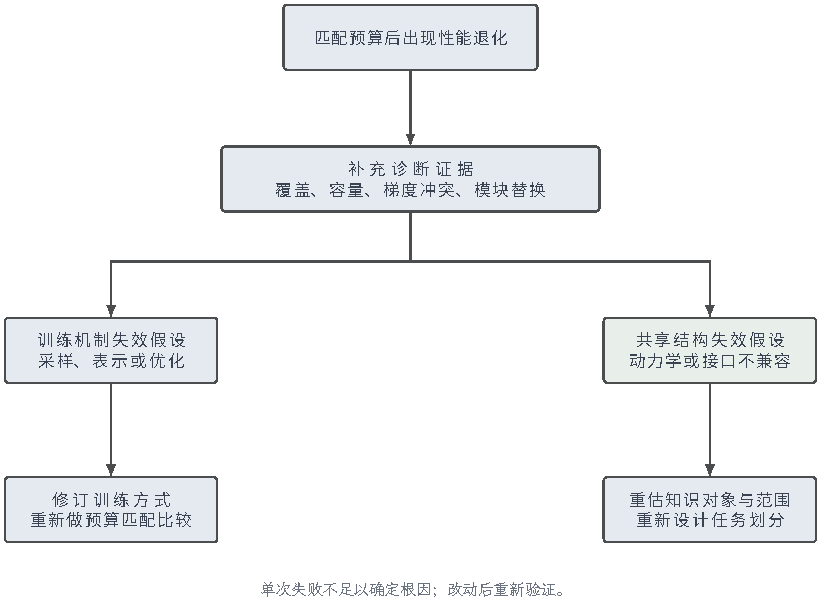
\includegraphics[width=139.019mm]{figures/10-reinforcement-learning/03-task-expansion-and-trustworthiness/tikz/rl-transfer-diagnosis.pdf}
 \caption{由退化结果形成可区分的诊断。分支表示待检验解释，不能只凭一次失败直接确定根因；训练问题修订采样、容量或优化，结构问题则重估共享对象及适用任务。图为本章诊断关系的原创示意。}
 \label{fig:rl-transfer-diagnosis}
\end{figure*}

单一基线可能容量不足，一次种子可能恰好失败，模块替换也可能同时增加容量。因此需要逐项控制差异，报告重复试验与不确定性，而不是见到改进就倒推唯一原因。共享结构一旦改变，原来的任务支持与组合假设也要重查，不能沿用旧条件下的泛化声明。

% Outline: 6.6.4
\subsection{由评测证据限定泛化与适应声明}
\label{sec:rl-transfer-claims}

同是“在新任务上成功”，支持内新终点上的直接执行，与无预告变风后的在线恢复，需要的证据不同。迁移声明应同时给出目标任务关系、可读取的任务描述与交互记录、适应预算和性能证据，才能让读者重建实际测试的问题。表~\ref{tab:rl-transfer-claims}~汇总本章导航变体分别能够支持的说法；这些结论以相应实验确实取得可靠证据为前提，本章教学数值本身不构成算法实验证据。

\begin{table*}[t]
 \centering\small
 \begin{tabularx}{\linewidth}{@{}>{\raggedright\arraybackslash}p{22mm}*{4}{>{\raggedright\arraybackslash}X}@{}}
  \toprule
  目标任务关系 & 可读任务描述与反馈 & 适应预算 & 评价证据 & 允许的结论\\
  \midrule
  支持内新目标 & 兼容的目标坐标 & 无反馈适应 & 任务级留出零样本回报 & 声明总体内的描述条件泛化\\
  未见目标与风组合 & 相同描述字段 & 固定$B,K,L,C$ & 留出联合组合的分组结果 & 指定因素与组合上的能力\\
  未见噪声范围 & 描述或获准历史 & 明确探测与更新 & 范围外分组、失败与误差 & 已测范围内的外推证据\\
  固定隐藏风向 & 无真实风标签，反馈逐步可见 & 探测、恢复、评价均计 & 辨识误差、适应回报与参照差额 & 规定描述与反馈条件下的固定任务适应\\
  变化风向序列 & 不提前见未来变化 & 按时间顺序持续交互 & 动态遗憾、检测延迟与恢复 & 指定变化预算及信号下的跟踪\\
  \bottomrule
 \end{tabularx}
 \caption{证据与声明的对应关系。支持内、组合、范围外、固定隐藏任务和变化任务不是逐级自动推出的能力；每一行都需要自身的任务划分与协议。}
 \label{tab:rl-transfer-claims}
\end{table*}

训练任务数量很大，但每项只改变同一地图的颜色时，测试高分仍不能证明新几何泛化。目标和风向都单独测过，但从未共同改变时，不能推断组合有效。若变化检测器提前读到了下一回合任务标签，快速恢复也不能支持无预告持续适应。这些反例没有否认已测分数，而是限定分数回答的问题。

还应区分平均能力与最低要求。对声明任务分布取得较高平均回报，不等于在所有允许扰动下都不低于某个阈值；后者需要明确扰动集合、风险或最坏情形准则，以及相应验证。鲁棒性与可信保证留到第~\ref{chap:rl-trustworthy}~章讨论，不能由本章经验泛化结果直接推出。

% Outline: 6.7
\section{本章小结}
\label{sec:rl-transfer-summary}

回到章首的小车：共同终止规则下换奖励目标，可以保留移动模型，却要按新奖励重算价值；若换终点还改变吸收规则，就连完整转移核也需要重查。地面变滑时，目标含义可以保留，旧后果预测却可能失效。能否迁移取决于复用对象所需的共享条件，以及新任务是否满足这些条件。参数形状相同、平均回报相近或任务编号相邻，都不能替代逐项检查。

训练得到的表示、模型、价值、策略初始化和技能，在部署中仍要结合描述、历史与权限，才能形成具体策略。固定参数可以通过记忆适应，参数更新需要获准且能支持目标估计的训练样本，持续交互只有在反馈有区分力且动作获准时，才可能取得区分候选任务所缺的观测或奖励。后继特征把共同动力学下的后果与奖励权重分开，GPI逐状态组合已有策略的候选动作；它们没有消除奖励类和策略覆盖的限制。贝叶斯任务更新则说明怎样用正确似然认识固定任务，不能直接累积过时证据来跟踪变化任务。

认识固定未知任务与追踪变化任务并不相同。每轮独立变化的两臂例子表明，计算或记忆无法补出缺失的当前最优臂提示。任务级划分、完整预算、匹配比较者和分层失败诊断，共同约束泛化与适应声明。伙伴与对手也会带来任务变化，但各自的目标与共同学习需要联合建模。第~\ref{chap:rl-multi-agent}~章将考察这些依赖，并把任务描述、反馈读取范围与适应预算的约定用于交互双方。

\chapter{多智能体协作和博弈}
\label{chap:rl-multi-agent}

前几章始终只有一个决策者，环境在它眼里是一套固定的物理规则。本章放宽这一前提：环境中同时存在多个会决策、而且可能也在学习的参与者。先看一个最日常的例子：两个人从窄通道的两端相向而行。同样是向前迈步，对方愿意等待时我就能通过，对方也往前冲时两人就可能堵在入口。也就是说，同一个动作的后果不仅取决于通道的物理规则，还取决于另一个人的选择；若对方也在学着避让，那么今天还奏效的策略，明天可能就不再管用。多智能体问题的本质，就是行动后果由所有人的选择共同决定，而各方的选择又可能随交互不断改变。

要在这种交互中套用价值学习，必须先想清楚三件事：要最大化的是谁的回报？每个人行动前能读到哪些观测、历史和消息？对方的策略会不会随交互而变化？这三者缺一不可。多方交互仍使用第\ref{chap:rl-overview}章已说明的策略、回报与价值，以及第\ref{chap:rl-learning}章的采样和更新工具，只是对象之间多了层层依赖：收益关系决定“怎样的行为才算好”，观测与消息的读取权限决定哪些策略真正能执行，联合经验用于估计行为后果，而策略一旦更新，又反过来改变下一批经验的来源。本章大致顺着这条依赖链展开——先搭共同设定、再按收益关系确定行为标准，然后讨论经验怎么采、后果怎么估、策略怎样一起更新，最后处理参与者变化以及如何评价与验证。估计后果时，可以同时保留双方动作、比较自身替代动作的后果，或直接预测伙伴会怎样行动；更新策略时可以沿收益梯度改进，也可以用历史策略来安排训练配对和响应对象。这些选择处理的是不同层面的依赖，并不互斥，可以组合使用。图\ref{fig:rl-multi-agent-map}画出这些依赖。

\begin{figure}[htbp]
  \centering
  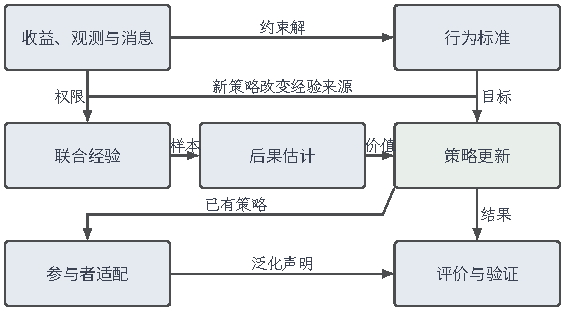
\includegraphics[width=95.652mm]{figures/10-reinforcement-learning/03-task-expansion-and-trustworthiness/tikz/rl-multi-agent-map.pdf}
  \caption{多智能体求解中的问题关系。实线连接约束、交互记录与后果估计的用途，外侧回路表示策略更新改变后续经验来源；底部的适配与评价检查行为标准在所声明参与者范围内是否成立。}
  \label{fig:rl-multi-agent-map}
\end{figure}

% Outline: 7.1
\section{收益、信息与参与者的共同设定}
\label{sec:rl-multi-agent-setting}

% Outline: 7.1.1
\subsection{用联合动作、转移与个体回报定义决策过程}
\label{sec:rl-multi-agent-process}

把通道截成一次“谁先通过”的竞争，可以得到一个确定性的教学任务。初态为两人都尚未通过的$s_{\text{入口}}$，另有“1先通过”“2先通过”和“碰撞”三个终止状态；两人都能观察当前状态，并读取自己的奖励。在入口，各人选择前进$F$或等待$W$。联合动作$(F,W)$使1先通过，两人的奖励依次为$(-1,-2)$；$(W,F)$使2先通过，奖励为$(-2,-1)$。$(F,F)$导致碰撞，双方各得$-4$并终止；$(W,W)$使系统留在入口，双方各得$-1$，下一步重新选择。三个终止状态都吸收，后续奖励为0。这里的数值是独立教学设定，不取自前几章的随机网格。

这个小任务把多人问题新增的依赖具体化：推动状态变化的是联合动作，每个人的奖励可以不同，观察权限也须逐人规定。一般环境还可能让奖励、后继观测和终止标记共同随机产生，因此需要一个联合生成模型。

\begin{definition}[多参与者序贯决策]
\label{def:rl-multi-agent-game}
给定正整数$m$、非空状态空间$S$、各人的非空行动空间$\mathsf A_i$与非空观测空间$\mathsf O_i$，均配备可测结构。设参与者集合为$\mathcal N=\{1,\ldots,m\}$，用$-i$表示除$i$之外的参与者，$\mathsf A_i(s)$为$i$在状态$s$中的非空合法动作集合，合法状态—联合动作对构成可测集合。各人动作组成$\bm a=(a_1,\ldots,a_m)\in\prod_i\mathsf A_i(s)$。以下各核与策略均可测，允许的合法策略集合非空。环境以从合法状态—联合动作对到$S\times\mathbb R^m\times\prod_i\mathsf O_i\times\{0,1\}$上概率测度的联合反馈核
\[
 K(\mathrm ds',\mathrm d\bm r,\mathrm d\bm o',\mathrm dd\mid s,\bm a)
\]
一次生成后继状态$s'$、个体奖励向量$\bm r=(r_1,\ldots,r_m)$、下一联合观测$\bm o'$及终止标记$d\in\{0,1\}$。共同转移核和期望奖励分别是这一联合律的边缘与条件均值：
\[
 \begin{aligned}
 T(B\mid s,\bm a)
 &=K\!\left(B\times\mathbb R^m\times\prod_i\mathsf O_i
              \times\{0,1\}\mid s,\bm a\right),\\
 R_i(s,\bm a)
 &=\int r_i\,K(\mathrm ds',\mathrm d\bm r,\mathrm d\bm o',\mathrm dd\mid s,\bm a).
 \end{aligned}
\]
其中$B$是$S$的可测子集，并要求各合法$(s,\bm a)$下$\int|r_i|\,\mathrm dK<\infty$。有限或可数空间中的积分按相应点质量求和。这里没有假设奖励、观测、后继状态和终止标记条件独立；若要使用因子化接口，须另行给出因子分解。

行动权限由局部历史$I_{i,t}$限定：它只包含$i$在动作$t$之前获准取得的观测、自身过去动作、可见奖励和已收到的消息。执行第$t$步联合动作后，联合反馈核先产生反馈，各人只能把协议允许其看见的部分写入$I_{i,t+1}$；策略产生的消息及其送达时刻另由通信协议规定。策略$\pi_i(a_i\mid I_i)$只依据该参与者获准取得的局部观测、消息和自身行动记录选择动作。记各人的策略合称为$\bm\pi$。初始分布$\mu_0$专指物理初态分布；下式的期望还固定初始观测、初始消息与公共信号的生成约定。要求每个参与者的折扣奖励和绝对可积，即$\mathbb E\sum_{t\geq0}\gamma^t|r_{i,t}|<\infty$；有界逐步奖励是充分条件。参与者$i$要评价的未归一化折扣回报为
\[
 J_i(\bm\pi)=\mathbb E_{\mu_0,\bm\pi}
 \left[\sum_{t=0}^{\infty}\gamma^t r_{i,t}\right],
 \qquad 0\leq\gamma<1.
\]
\end{definition}

把所有人的策略合在一起称为联合策略$\bm\pi$。它能不能写成各人策略的乘积，取决于动作是怎样产生的：给定联合历史$\bm I$后，若各人独立地各自随机化，才有$\bm\pi(\bm a\mid\bm I)=\prod_i\pi_i(a_i\mid I_i)$；若行动前先广播过一个公共随机信号$c$（比如抽签决定谁先走），那么这种独立性只能在给定$c$之后使用。把信号平均掉，得到$\sum_c p(c\mid\bm I)\prod_i\pi_i(a_i\mid I_i,c)$，一般不能再拆成各自边缘分布的乘积。若所有人都只行动一次，可以把每组联合动作的收益排成一张矩阵，得到矩阵博弈：每个格子对应一个联合动作，格子里写各方收益。加入共同状态和转移后，就相当于“在每个状态上各摆一局矩阵博弈，而这一局的动作结果又决定下一局发生在哪个状态”，这称为随机博弈（stochastic game），Shapley 建立了其完全可观测形式的经典理论\scite{rl1-shapley1953-games}。

一个自然的简化念头：既然真正要优化的只是我自己的策略，能不能把其余人也当成“环境”的一部分，继续套用单人 MDP？答案是有条件的——当其他人都使用固定的状态条件策略、并且给定$s$后他们的联合动作与我的动作独立随机化时，可以把他们各种动作出现的概率当作随机转移的一部分，按概率把转移与奖励加权平均掉。这一步边缘化给出$i$实际面对的过程：
\begin{align}
 T_i^{\bm\pi_{-i}}(s'\mid s,a_i)
 &=\sum_{\bm a_{-i}}\bm\pi_{-i}(\bm a_{-i}\mid s)
 T(s'\mid s,a_i,\bm a_{-i}),\label{eq:rl-multi-agent-induced}\\
 R_i^{\bm\pi_{-i}}(s,a_i)
 &=\sum_{\bm a_{-i}}\bm\pi_{-i}(\bm a_{-i}\mid s)
 R_i(s,a_i,\bm a_{-i}).\nonumber
\end{align}
在通道中，对方以概率$q$等待时，自己前进的通过概率为$q$，期望即时收益为$q(-1)+(1-q)(-4)=-4+3q$。若对方学习后把$q$从$0.8$降到$0.2$，这两个量都会改变，尽管共同的$T$和$R_i$没有变化。因而，对$i$而言过程不再平稳，可能仅仅是因为边缘化时使用的对方策略变了，而非物理环境发生漂移。

使用式\eqref{eq:rl-multi-agent-induced}时，要检查的是$\mathbb P(\bm a_{-i}\mid s,a_i)=\bm\pi_{-i}(\bm a_{-i}\mid s)$，而不是要求其他人彼此独立。公共信号若使双方动作相关，观察到自身动作也可能改变对其他动作的判断，不能直接用其边缘分布加权；应先把信号纳入条件，再检查等式。另一个限制来自记忆：对方若按过去碰撞次数调整让行概率，当前位置就不足以预测其下一动作。需要把相关记忆或类型纳入充分状态，或者在历史上定义过程，才能讨论相应的评价与收敛；原有平稳MDP结论不能直接沿用。

% Outline: 7.1.2
\subsection{不同收益关系下的合作、零和与一般和问题}
\label{sec:rl-multi-agent-payoffs}

保留入口和两种动作，改变奖励就会改变要解决的问题。若两人共享奖励，可另设碰撞$-2$、都等待$-1$、恰好一人前进$2$，目标是共同避免冲突并尽快通行。若只比较谁先通过，可让$(F,W)$给第一人$1$，$(W,F)$给第一人$-1$，其余为$0$，第二人取相反收益。若各人承担自己的时间成本，则等待者可能比先行者损失更多，而碰撞同时损害双方。以上是分别说明三种收益关系的教学设定，不是同一奖励表。

这三种奖励安排恰好对应多智能体中三类典型的收益关系，也是后面判断“策略是否变好”的三种不同标准。\term{完全合作}（fully cooperative）意味着所有人评价的是同一个回报目标，相当于同一支队伍：把蛋糕做大对每个人都有利。\term{两人零和}（two-player zero-sum）要求每个结果满足$r_{1,t}+r_{2,t}=0$，即一方的每一分收益恰好是另一方的损失；对整条轨迹求和取期望便有$J_2=-J_1$，最典型的就是零和对抗。\term{一般和}（general-sum）则不限制各收益之间的关系，可以同时含有共同利益与个人冲突——通道里双方都不希望碰撞，却又都想先通过。还要特别强调：目标相同不代表两人能读到相同的观测与消息，更不保证两个各自独立学习的人能自发形成彼此兼容的让行约定。表\ref{tab:rl-multi-agent-payoffs}据收益关系列出对应的行为标准，使后续“改进”有明确的比较对象。

\begin{table}[htbp]
 \centering
 \begin{tabularx}{\linewidth}{@{}l >{\raggedright\arraybackslash}X >{\raggedright\arraybackslash}X@{}}
 \toprule
 收益关系 & 标准与单方偏离 & 额外社会选择\\
 \midrule
 完全合作 & 在允许的局部观测与消息条件下最大化共同$J$；单方改动也按共同收益计 & 若存在多个最优策略，仍需选择兼容约定\\
 两人零和 & 最大化最坏收益；偏离检验可被利用的程度 & 价值标准已给定，风险限制可另设\\
 一般和 & 各自偏离是否获利；可另优化福利 & 必须另定福利、公平及取舍\\
 \bottomrule
 \end{tabularx}
 \caption{同一任务接口在不同收益关系下的行为标准。完全合作可比较共同回报，零和可比较最坏收益，一般和须另行指定社会目标。}
 \label{tab:rl-multi-agent-payoffs}
\end{table}

一般和中，总收益与个人激励可能冲突。总收益很高的结果可能诱使一人立即偏离；没有人愿意单方偏离的结果也可能使双方收益都很低。奖励求和可以定义一种福利指标，却既不规定收益如何分配，也不保证个人愿意维持该结果。评价时必须把福利、分配和稳定性分别说明。

% Outline: 7.1.3
\subsection{不同行动、观测与通信时序下的信息结构}
\label{sec:rl-multi-agent-information}

收益关系确定之后，还要确定作出选择时知道什么。通道中的“我先走”若在对方行动前送达，可以支持本轮避让；若延迟一轮，只能进入$I_{i,t+1}$。图\ref{fig:rl-multi-agent-timing}为此分别标出观测、发信、收信、行动和反馈。训练日志事后收齐消息，不意味着动作$t$可以使用它。行动本身也有时序限制：顺序行动的后手可能观察先手动作，同时行动的双方则不能据本轮尚未提交的对方动作决策。

\Needspace{16\baselineskip}
实现时，依次调用程序不等于允许依次观察行动。PettingZoo以统一接口支持多类多智能体环境，其中智能体—环境循环（agent environment cycle, AEC）接口逐个调用参与者。用它实现同时行动任务时，仍要屏蔽本轮其他人尚未共同提交的动作，否则调用顺序就意外地让后手提前读到了本轮其他人的动作\scite{rl7-terry2021}

\begin{figure}[htbp]
 \centering
 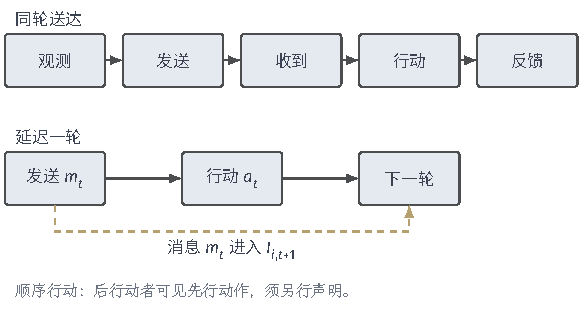
\includegraphics[width=98.616mm]{figures/10-reinforcement-learning/03-task-expansion-and-trustworthiness/tikz/rl-multi-agent-timing.pdf}
 \caption{消息何时进入策略输入。实线表示本轮可读取的观测与已送达消息，虚线表示下一轮才送达的消息；顺序行动还可能允许后手观察先行动作，这一权限不属于同时行动。}
 \label{fig:rl-multi-agent-timing}
\end{figure}

确定送达时刻后，还须规定消息携带什么。通信模型CommNet让参与者发送连续向量，把同伴发送的消息聚合成一个表示，再将其用于协作决策。这些表示能成为本轮策略输入的前提仍是动作前按协议送达，网络中的聚合运算不能替代实际通信权限\scite{rl7-sukhbaatar2016}

前面的讨论默认每个人都能看到完整状态，但真实场景往往不是这样：过道里看不到拐角后面是否有人，扑克玩家也看不到对手的底牌。于是需要给每个参与者单独规定他能看到的观测，而不是假设大家共享同一个$s$；各人看到不同信号的随机博弈称为\term{部分可观测随机博弈}（partially observable stochastic game, POSG）。把定义\ref{def:rl-multi-agent-game}中“下一观测”的条件单独取出，常将定义\ref{def:rl-multi-agent-game}中的观测条件边缘记为联合观测核$K_o(\bm o'\mid s',\bm a)$，并另给初始观测分布，说明状态怎样生成每个人看到的信号。采用这一简化接口，意味着观测边缘在给定$(s',\bm a)$后不再依赖旧状态；它不表示观测与奖励或终止反馈条件独立，完整耦合关系仍由$K$规定。局部观测$o_i$不等于完整状态$s$。若进一步共享团队奖励、并要求各策略只使用自己的历史，就得到\term{分散部分可观测马尔可夫决策过程}（decentralized POMDP, Dec-POMDP）：大家为同一个回报行动，却分别依据各自的观测、动作、奖励历史与合法消息作出选择。这里的困难超出单人 POMDP：即使把各人的观测合起来足以恢复状态，每个人在决策时也没有权限读取别人的观测。通信可以表示为动作的一部分或单独的消息阶段，顺序行动可以在状态中标记当前行动者；这些建模方式都必须保留实际观测范围和消息送达时序的限制\scite{rl7-bernstein2002}。

局部观测和可读行动历史对策略的限制可以用一个有限隐藏牌面游戏说明。这不是标准扑克；以下规则定义了全部随机性与收益。机会方以各$1/2$的概率给参与者1发高牌$H$或低牌$L$，只有1看见牌，两人先各投入一单位。1先选择下注$B$或过牌$K$：下注后由2选择弃牌$F$或跟注$C$；过牌后由2选择过牌$K$或下注$B$。若2也过牌，立即摊牌；若2下注，1再选弃牌$F$或跟注$C$，随后结束。摊牌时，高牌由1赢，低牌由2赢；无人加注时胜者净得$1$，跟注后胜者净得$2$。有人弃牌时，未弃牌者净得$1$。另一人取相反净收益，全局只有终局收益，不设折扣。

图\ref{fig:rl-multi-agent-card-tree}把这些规则展开成完整历史树：顶部机会节点生成牌面，圆节点表示决策，叶节点给出1的净收益。面对1首次下注，2不能区分高牌与低牌分支上的两个节点，因而它们属于同一\term{信息集}（information set），即依据该参与者已取得的观测、动作、奖励和消息无法区分的一组完整历史。2必须在两处使用相同的跟注概率；按牌面分别设概率就使用了参与者2并未看到的牌面。相反，2能够看见1是下注还是过牌，这两种情形必须属于不同的信息集。

\begin{figure}[htbp]
 \centering
 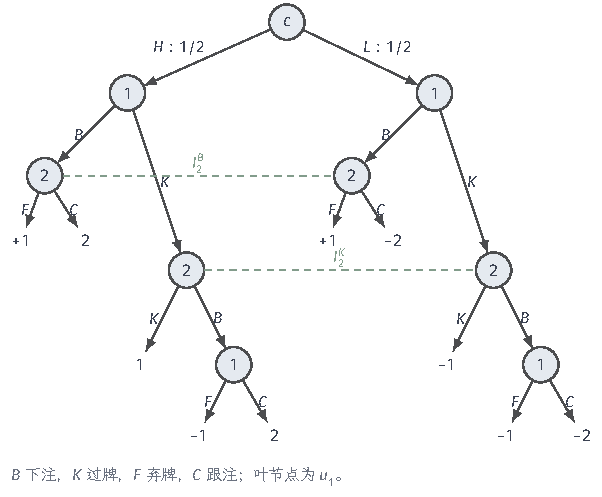
\includegraphics[width=101.946mm]{figures/10-reinforcement-learning/03-task-expansion-and-trustworthiness/tikz/rl-multi-agent-card-tree.pdf}
 \caption{隐藏牌面教学游戏的完整历史树。虚线各自连接2面对下注、面对过牌时不能区分的节点；1知道牌面，其节点不跨牌面合并。叶节点标1的净收益，2取相反数。}
 \label{fig:rl-multi-agent-card-tree}
\end{figure}

这里引入的\term{信息集}（information set），直观上就是“在某个参与者看来无法区分的一组完整局面”：处在同一信息集的节点，对他而言可能给出完全相同的观察和历史，所以他必须在这些节点上使用同一套动作概率。但信息集也不能抹掉参与者自己的记忆。\term{完全回忆}（perfect recall）要求同一信息集里的所有历史，都具有相同的“自己过去知道过什么、做过什么”序列。

% Outline: 7.1.4
\subsection{信息权限与联合策略表示}
\label{sec:rl-multi-agent-permissions}

若由一个能取得全局状态与各人历史的控制器选择联合动作，就可以集中决策。困难在于训练与部署可读取的变量不同：训练通常在仿真器或服务器上进行，可以记录全局状态、联合动作和各人的历史；真实部署时，每个人却只有局部传感器，不能即时读取其他人的位置、局部观测与历史，通信也可能受限。这些集中变量可以帮助训练评论家，但执行策略仍不能依赖部署时读不到的变量。\term{集中训练、分散执行}（centralized training with decentralized execution, CTDE）正是把这两种权限分开：训练时允许用全局状态、联合动作或其他人的历史来估计价值，行动策略在部署时则只能读取本地历史及获准送达的消息。

\begin{figure*}[htbp]
 \centering
 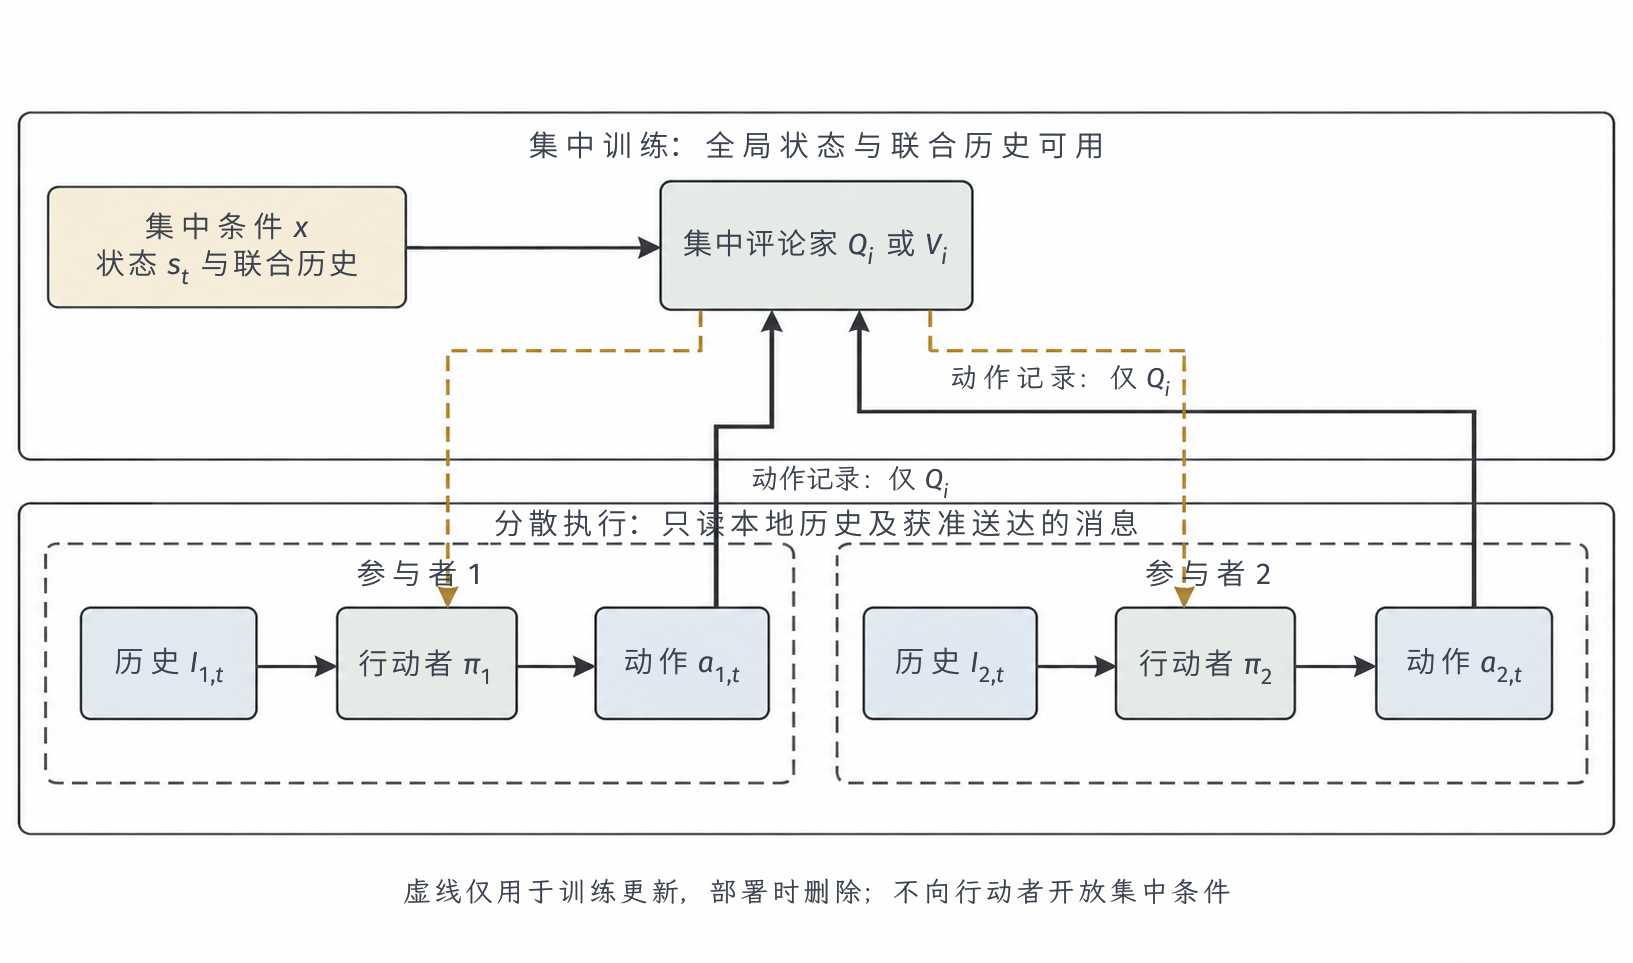
\includegraphics[width=157.400mm]{figures/10-reinforcement-learning/03-task-expansion-and-trustworthiness/generated/rl-multi-agent-ctde/figure.png}
 \caption{CTDE中的集中训练与分散执行。上区的集中评论家可使用全局状态及联合历史，下区各行动者只使用本地历史和获准消息。向评论家上送的当前动作仅用于$Q_i$，估计$V_i$时不取当前动作作为条件；部署时删除训练虚线，也不向行动者开放集中条件。两个参与者仅为示例。}
 \label{fig:rl-multi-agent-ctde}
\end{figure*}

在执行权限相同的前提下，还可以选择是否共享参数。若两人的观测、动作和角色含义兼容，共享$\pi_{\bm\theta}(a_i\mid I_i)$可让同一函数服务两人，但不会让他们读取对方的局部观测或消息。加入身份编码$e_i$后，网络可按编号形成“1先走、2等待”的约定；身份重排却可能使该约定失效。独立参数容纳不同动作接口或角色，但需分别存储和拟合各人的网络，并寻找能彼此配合的策略组合。参数量和训练样本需求还取决于网络结构与任务，不能仅由参数独立就断言样本成本更高。身份是否必要，应由任务中的角色含义决定。

通信也可以参与参数学习。可微智能体间学习（differentiable inter-agent learning, DIAL）在训练时通过可微信道传递梯度，使发送者得到关于消息用途的反馈，部署时则改用受限的离散消息。连续训练近似与实际离散信道并不相同，量化可能改变接收到的消息内容，因此仍要检查部署消息能否支持学到的协调行为\scite{rl7-foerster2016}

要检查这种训练与执行差异，协议必须说明谁向谁发送什么、何时送达，以及花费多少带宽。表\ref{tab:rl-multi-agent-communication}比较四种可与CTDE组合的接口。能否通过消息反向传播属于训练计算条件，链路延迟、带宽和接收权限则约束实际执行，两者不能相互替代。

\begin{table}[htbp]
 \centering
 \begin{tabularx}{\linewidth}{@{}l >{\raggedright\arraybackslash}X >{\raggedright\arraybackslash}X@{}}
 \toprule
 接口 & 发送者、接收者与内容 & 时序、带宽及训练／执行条件\\
 \midrule
 固定协议 & 每人向指定邻居发角色或让行码 & 动作前收信；固定比特数；两阶段协议均保持\\
 可微通信 & 所有人向聚合器或同伴发实向量 & 每轮一至多次交换；向量维数固定；执行须保留信道\\
 离散消息 & 每人向获准接收者发有限字母表符号 & 训练可用连续松弛；执行量化后重新核验\\
 图消息传递 & 节点向图邻居发嵌入或定向消息 & 边数与轮数决定带宽；部署只能使用可发现的边\\
 \bottomrule
 \end{tabularx}
 \caption{四种消息接口的执行条件。比较时须同时说明发送者与接收者、消息内容、送达时刻及通信成本，而不只报告训练中是否可微。}
 \label{tab:rl-multi-agent-communication}
\end{table}

若并非所有人都需要同一条消息，可以进一步学习发送对象。定向多智能体通信（targeted multi-agent communication, TarMAC）用定向寻址计算接收权重，让不同接收者聚合不同内容。它解决的是“消息给谁”，可以与消息内容的表示、训练信道的选择共同使用，但仍须符合部署的接收权限\scite{rl7-das2019}

% Outline: 7.1.5
\subsection{不同数据访问与参与者变化方式下的学习问题}
\label{sec:rl-multi-agent-access}

相同的两人通道，还会因交互记录的采集、访问权限和对方变化方式而形成不同学习问题。对方遵守固定避让规则时，学习者可以探索其响应；双方共同训练时，刚估计的规则下一轮可能已改变；从历史策略库抽样时，每场经验还取决于抽到了哪个版本。表\ref{tab:rl-multi-agent-access}将参与者条件与记录访问权限交叉列出。其中“可改变”只指学习者按协议能控制的因素，第三方主动改变策略不属于学习者的采集权限。

\begin{table}[htbp]
 \centering
 \begin{tabularx}{\linewidth}{@{}l >{\raggedright\arraybackslash}X >{\raggedright\arraybackslash}X >{\raggedright\arraybackslash}X@{}}
 \toprule
 参与者条件 & 在线访问 & 固定联合日志 & 有限批次访问\\
 \midrule
 固定伙伴 & 可改自身行为，伙伴不变 & 不可重采；还原固定版本 & 批间改自身，批内固定\\
 同步学习者 & 可按约定更新双方 & 仅观察历史更新，不能重放新响应 & 批间同步更新，批内冻结\\
 群体抽样 & 可改获准的抽样分布 & 只能使用已记录群体支持 & 批间改抽样，批内固定\\
 主动适应者 & 自身动作可诱发其响应，未必可控 & 响应机制可能不可识别 & 须声明对方是否随批内历史更新\\
 \bottomrule
 \end{tabularx}
 \caption{记录访问权限和参与者变化共同限定可做的采集。有限批次若包含对方的批内适应，整批就不能被描述为固定联合策略产生的交互记录。}
 \label{tab:rl-multi-agent-access}
\end{table}

多智能体建模不要求所有参与者都在学习：即使只优化一个策略，也须表示其他行为怎样共同决定结果。反过来，同时运行多个固定规则代理或多个语言模型角色，并不能说明发生了强化学习。还需给出被优化的策略、交互产生的反馈和更新所针对的回报。“多人对话”描述的是交互形式，不能代替这些学习条件。

% Outline: 7.2
\section{不同收益关系下的行为标准}
\label{sec:rl-multi-agent-solutions}

模型建好了，但“回报提高”在不同收益关系下含义完全不同：合作时是共同蛋糕变大，零和时是最坏情况下不吃亏，一般和时则要问有没有人愿意单方面改变行为。因此在讨论学习之前，必须先选定衡量行为的标准。下面保留有限两动作的教学接口，分别考察共同目标下的团队最优、零和对抗中的最坏情形价值、以及一般和博弈中的单方偏离稳定性。三者对应的收益关系不同，不能把其中一种意义上的“改进”当成另一种标准也得到了满足。

% Outline: 7.2.1
\subsection{共同目标下的联合最优标准}
\label{sec:rl-multi-agent-team}

共享回报时，目标函数很直接：最大化共同的$J(\bm\pi)$。但这里有一个初学者极易忽略的限制——可搜索的策略范围只能是部署时真正可执行的$\Pi_{\text{分散}}$，其中每条策略都必须满足局部观测范围、消息时序和公共随机性的约束。训练服务器可以用全局状态或联合历史来帮助估计、帮助求解，却不能因此让部署时的行动者直接读到这些变量。一个能看到全局的“中央大脑”当然可能做得更好，下面的包含关系就给出这种集中求解相对分散最优值的上界。

\begin{theorem}[集中与分散策略的可行集合]
\label{thm:rl-multi-agent-inclusion}
设奖励有界且$0\leq\gamma<1$。若集中控制器在每个决策时刻取得分散系统的全部可用历史，还能模拟其私有随机性、公共随机性和合法通信，就能为每个分散策略生成相同的轨迹分布。按所实现的分布识别策略，有
\[
 \Pi_{\text{分散}}\subseteq\Pi_{\text{集中}},
 \qquad
 \sup_{\bm\pi\in\Pi_{\text{分散}}}J(\bm\pi)
 \leq
 \sup_{\pi\in\Pi_{\text{集中}}}J(\pi).
\]
\end{theorem}
\begin{proof}
对任意分散策略$\bm\pi$，让集中控制器分别保存各人的局部历史，并在每一时刻按原协议产生公共信号、私有随机数和消息，再调用各$\pi_i$生成联合动作。这样既不改变随机机制，也不向局部策略额外提供其他人的观测或消息。模拟从相同的初始历史分布开始；若直到$t$的联合历史分布相同，相同策略调用就产生相同的条件动作分布，未变的联合反馈核和合法消息生成、送达协议继而产生相同的$t+1$历史分布。这里的反馈包括各人可见的奖励、观测与终止标记，不能只比较状态边缘。归纳可得所有有限轨迹分布一致。有界奖励与$\gamma<1$保证相应折扣回报期望一致，所以每个分散系统可达的回报都能由集中控制器实现。对两种可达集合取上确界，便得到不等式；若有限问题中最优策略存在，上确界可写成最大值。
\end{proof}

集中上界不一定能分散实现。设通行前产生均匀二值信号$c\in\{0,1\}$，两个值的概率各为$1/2$，只有两人都选$c$时团队得$1$，否则得$0$。集中控制器看到$c$，每次都能得$1$。对分散双方，假设各自观测均与$c$独立，不许互传观测，使用的随机数也独立于$c$及双方观测。允许公共随机数只能帮助两人协调，不能让任一人知道$c$；其动作仍与$c$独立。成功事件包含在第一人选对的事件中，故
\[
 \mathbb P(a_1=a_2=c)\leq\mathbb P(a_1=c)=\frac12.
\]
这里仅使用每个人动作与$c$的独立性，没有把逐个独立扩大为联合观测或联合动作的独立性。固定都选0可以达到$1/2$这一上界。若允许在行动前广播$c$，局部策略才有条件按信号选择，分散最优值也才恢复为1。

因此，声称团队最优时须同时给出回报目标和允许的观测、历史与消息条件。一次成功协调仅说明找到了一个有效行为，参数空间的局部最优也不等于整个可行策略集合的最优。若原问题的个人收益不同，更不能在没有另定目标的情况下把它改写成团队最大化。

% Outline: 7.2.2
\subsection{零和对抗下的极小极大标准}
\label{sec:rl-multi-agent-minimax}

先从直觉理解为什么在零和对抗中，确定性动作往往不可取、必须随机化。用一个“猜对方选哪侧”的两动作任务说明。
\begin{equation}
 \bm A=
 \begin{pmatrix}1&-1\\-1&1\end{pmatrix}.
 \label{eq:rl-multi-agent-matching}
\end{equation}
第一人固定选任一侧，第二人总能选一列使其收益为$-1$；第一人均匀随机时，两列的期望却都为0。因而随机化的用途是抵御对手对行动偏好的利用，而不是减少单条轨迹的不确定性。

把这个例子推广。对一般收益矩阵$\bm A\in\mathbb R^{p\times q}$，令$\bm x\in\Delta_p$、$\bm y\in\Delta_q$分别为两人在纯动作上的概率分布，这样的随机化称为\term{混合策略}（mixed strategy）；其中$\Delta_p$表示所有分量非负且总和为 1 的$p$维概率向量，$\Delta_q$同理。按行、列概率给各格收益加权，得到$\bm x^\top\bm A\bm y$，由第一人最大化、第二人最小化。固定对方策略后，自身的最优选择称为\term{最佳响应}（best response）；若两人都固定对方策略、谁也无法再通过单方面改变来提高收益，这样的组合就称为\term{鞍点}（saddle point）——在收益曲面上，沿一方方向是极大、沿另一方方向是极小，形如马鞍。要抵御对手利用自己的偏好，第一人不能只针对某个平均对手拿高分，而必须保证在所有允许的对手策略下都能守住一个收益下界。于是有两种设想博弈顺序：第一人先公开自己的混合策略、第二人随后针对它最小化，第一人在这个前提下取最大化；或者反过来。直观上“先承诺、后被针对”似乎吃亏，但在有限动作且双方都允许任意混合策略的条件下，两种顺序恰好给出同一个博弈值。

对正整数$p,q$及收益矩阵$\bm A\in\mathbb R^{p\times q}$，若双方允许全部行、列混合策略$\Delta_p,\Delta_q$，收益$\bm x^\top\bm A\bm y$对双方策略双线性，则有限零和极小极大结论给出
\[
 \max_{\bm x\in\Delta_p}\min_{\bm y\in\Delta_q}\bm x^\top\bm A\bm y
 =\min_{\bm y\in\Delta_q}\max_{\bm x\in\Delta_p}\bm x^\top\bm A\bm y.
\]
双方的最优混合策略都存在，组成鞍点。
这个结论把有限双线性零和问题的两种优化次序接成同一个博弈值。它让后继状态上的矩阵收益得到确定的最坏情形价值，供控制备份调用；并未说明有限样本或神经网络更新能求出这一价值。有限矩阵博弈、相关建议、遗憾与平均策略的一般分析可参考\BookChapterRef{chap:game-theory-and-multi-agent-decision}{卷2《数学准备：概率、因果与决策》“多方策略的响应与演化”章}。允许全部混合策略是关键条件；把策略限制为非凸神经网络参数类后，允许集合已经改变，不能直接沿用等式。

上述阶段博弈值可以直接嵌入多步决策。对完全可观测的两人零和折扣随机博弈，把$Q(s,\cdot,\cdot)$看成状态$s$上的一张收益矩阵，用$\operatorname{val}Q(s)$表示它的极小极大值。即时奖励之后，双方在后继状态仍按最坏情形标准选择，于是控制备份就是把单人备份里的“对动作取最大”换成“对联合矩阵取极小极大值”：
\begin{equation}
 (\mathcal B Q)(s,\bm a)
 =R_1(s,\bm a)+\gamma\sum_{s'}T(s'\mid s,\bm a)
           \operatorname{val}Q(s').
 \label{eq:rl-multi-agent-minimax-backup}
\end{equation}
极小极大Q学习（Minimax-Q）用一次采样中的$r_{1,t}+\gamma\operatorname{val}Q(s_{t+1})$替代转移期望，再按步长$\alpha_t$更新当前表项。若奖励为1、后继博弈价值为0，旧值0.4以步长0.5向目标1移动，得到0.7。与单智能体只取动作最大值不同，每个后继价值都需要求解阶段线性规划；这一运算使Minimax-Q的备份反映对手的最坏响应\scite{rl7-littman1994}

这给出了目标的计算依据，还没有给出任意实现的收敛保证。表格分析另需有界奖励、各状态联合动作充分访问、合适的随机逼近步长和正确的阶段价值求解。深度逼近改变估计误差，局部观测改变状态条件，共同学习又可能改变状态与联合动作的访问覆盖；这些情形都需单独分析。

% Outline: 7.2.3
\subsection{一般和博弈下的均衡与社会目标}
\label{sec:rl-multi-agent-equilibria}

双方收益并不严格相反时，一个稳定性问题是：给定其他人都不变，我单方面换成别的策略能不能获益？例如两人各选左$L$或右$R$作为让行约定，同选一侧时双方各得2，选不同侧时双方各得0。这是一次行动后即终止的协调博弈，收益表为
\[
 \begin{array}{c|cc}
       &L&R\\ \hline
 L&(2,2)&(0,0)\\
 R&(0,0)&(2,2)
 \end{array}.
\]
若双方都选左，任一人单独改选右就会把自己的收益从2降到0；双方都选右也一样。稳定性在此检查的是单方改变，不要求两个稳定约定中必须选出唯一一个。

一般地，给定正整数$m$、各人的非空有限动作集$\mathsf A_i$及收益函数$u_i:\prod_j\mathsf A_j\to\mathbb R$。各人独立选择混合策略$\pi_i\in\Delta(\mathsf A_i)$，联合分布为$\bm\pi=\prod_i\pi_i$。若对每个参与者$i$和每个替代混合策略$\pi_i'\in\Delta(\mathsf A_i)$都有
\[
 \mathbb E_{\bm\pi}[u_i(\bm a)]
 \geq \mathbb E_{\pi_i'\prod_{j\ne i}\pi_j}[u_i(\bm a)],
\]
就称$\bm\pi$为\term{Nash均衡}（Nash equilibrium）。它将“其他人不变”写成固定$\bm\pi_{-i}$，将“任何单方改变都无利可图”写成对全部$\pi_i'$的不等式。在上述协调博弈中，都左与都右都是纯策略Nash均衡。
若由联合分布$q(\bm a)$产生动作建议，\term{粗相关均衡}（coarse correlated equilibrium, CCE）要求在看到建议之前改用固定动作也不能获利：
\[
 \mathbb E_q[u_i(\bm a)-u_i(b_i,\bm a_{-i})]\geq0
 \quad\text{对所有 }i,b_i.
\]
\term{相关均衡}（correlated equilibrium, CE）进一步允许根据收到的自身建议选择替代动作，要求
\[
 \sum_{\bm a_{-i}}q(a_i,\bm a_{-i})
 [u_i(a_i,\bm a_{-i})-u_i(b_i,\bm a_{-i})]\geq0
 \quad\text{对所有 }i,a_i,b_i.
\]

两个建议标准的区别在于偏离决定的时刻：CCE只比较事前选定的固定动作，CE还比较收到某个建议之后的替换，故CE约束更强。定义中的CE式没有除以建议概率，罕见建议带来的收益差仍按发生概率计权。Nash限定独立随机化，CE与CCE则允许联合建议相关。在上述协调博弈中，以各$1/2$概率建议双方都左或都右可以形成CE；将其边缘化后再独立抽样，却有一半概率失配。联合分布中的相关建议因此是行为标准的一部分。

当前两动作协调例说明联合建议怎样避免失配，还不能展示CE与CCE的严格差别。每位参与者都只有两个动作时，换成某个固定动作的CCE约束已经包含唯一的非平凡建议替换。下面增加第三个动作，才把两种偏离权限分开。

\begin{example}[事前固定偏离与收到建议后的偏离]
  \label{ex:rl-multi-agent-ce-cce}
  参与者1有动作$A,B,C$，参与者2有动作$L,R$。参与者1的收益为
  \[
    \begin{array}{c|rr}
          &L&R\\ \hline
      A& 0&-1\\
      B&-1& 0\\
      C& 1&-1
    \end{array},
  \]
  参与者2的收益恒为0。联合建议以各$1/2$概率给出$(A,L)$或$(B,R)$，照做时参与者1的期望收益为0。如果事前固定改选$A,B,C$，期望收益分别为$-1/2,-1/2,0$，都不能提高收益；参与者2也没有获利偏离，因此该建议分布满足CCE。

  但参与者1收到建议$A$时，已知道对方收到$L$。此时从$A$改为$C$会把收益从0提高到1，违反CE约束。这一偏离的未条件化期望获利为$1/2$，也直接违反定义中的CE不等式。因而CCE允许的分布可以被CE排除，原因是偏离者能否利用已经收到的建议。
\end{example}

有限个参与者、各人非空有限纯动作集且允许全部混合策略时，至少存在一个混合Nash均衡；这一存在性结论用于确认上述行为标准并非空要求。它并未保证高效计算，也未保证任意学习过程都会收敛到均衡\scite{rl7-nash1950}

表\ref{tab:rl-multi-agent-equilibria}比较这些标准的偏离对象。用于多步问题时，偏离者可能同时改变后续行为，因此“替代动作”须扩展为从全部相关历史到动作的\emph{完整策略}；若只检查受限的状态条件偏离，也须明确这一限制。即使某个已访问状态满足阶段CE，后续策略改变仍可能提高整个轨迹的回报，不能据此宣称序贯稳定。

\begin{table}[htbp]
 \centering
 \begin{tabularx}{\linewidth}{@{}l >{\raggedright\arraybackslash}X >{\raggedright\arraybackslash}X@{}}
 \toprule
 标准 & 偏离对象与信号 & 保证与未规定部分\\
 \midrule
 Nash & 固定对手后换自身策略；独立随机化 & 无单方收益改进；未最大化福利\\
 CE & 根据自己收到的建议换动作 & 无建议条件偏离；需合法相关信号\\
 CCE & 看建议前改为固定动作 & 无事前固定偏离；不排除条件偏离\\
 福利目标 & 按给定聚合函数选联合结果 & 可比较社会收益；不自动保证稳定或公平\\
 \bottomrule
 \end{tabularx}
 \caption{行为标准所检查的偏离与留下的选择。表中动作条件针对固定阶段博弈；用于序贯问题时，需要声明完整策略偏离还是某个受限偏离类。}
 \label{tab:rl-multi-agent-equilibria}
\end{table}

Nash Q学习（Nash Q-learning, Nash-Q）将阶段Nash标准用于多步目标：在后继状态的各人价值矩阵中选取均衡$\bm\sigma^*(s')$，按该均衡的联合动作概率加权各人的后继价值，得到
\[
 y_i=r_i+\gamma\sum_{\bm a'}\bm\sigma^*(\bm a'\mid s')
                         Q_i(s',\bm a').
\]
例如，在后继协调矩阵中选“都左”，各人后继值均为2；即时奖励0、$\gamma=0.9$时，目标就是1.8。若多个阶段均衡给出不同收益，目标将依赖选取规则；规则的不连续还可能改变更新动态。Nash-Q原文的收敛分析要求特殊的阶段均衡条件，存在性本身不能支持一般深度Nash-Q的收敛声明\scite{rl7-hu2003}

% Outline: 7.3
\section{多智能体的联合经验获取}
\label{sec:rl-multi-agent-data}

行为标准定下来之后，紧接着的问题是：要用什么样的联合交互记录才能估计它？多智能体在这里有一个单人问题没有的特殊困难——每个人都试过自己的动作，并不等于“团队”试过所需的动作组合。在通道里，两个人各自都单独前进过很多次，但“恰好一人前进、一人等待”这种关键组合可能从未同时出现。因此采集方案不能只规定每人探索什么，而要从待估量出发，规定参与者、行动前可读的历史和他们实际采取的联合行为，再回头检查这批记录能支持什么结论。若只有一份固定日志，则整个过程要从还原它的生成条件开始，不能假设还能重新采集。

% Outline: 7.3.1
\subsection{联合经验需求与采集方案的确定}
\label{sec:rl-multi-agent-collection-plan}

评价现有让行团队，需要部署伙伴分布下的当前策略回报；寻找自身改进，需要比较候选行为；检验单方偏离，还需要候选完整策略可能到达的后续状态。即使轨迹数量相同，对这三个任务也可能提供截然不同的支持。表\ref{tab:rl-multi-agent-data-needs}据此列出联合行为需求与可以控制的采集因素。

\begin{table}[htbp]
 \centering
 \begin{tabularx}{\linewidth}{@{}l >{\raggedright\arraybackslash}X >{\raggedright\arraybackslash}X@{}}
 \toprule
 待估量 & 所需联合行为与参与者范围 & 可控因素与预算\\
 \midrule
 当前团队回报 & 当前联合策略及部署伙伴分布 & 固定策略，重复独立回合，预算按回合计\\
 自身改进价值 & 固定或条件化伙伴下的候选自身动作 & 探索强度与起点；按联合环境步计\\
 单方偏离收益 & 原对手固定，完整候选响应的轨迹 & 响应训练、验证分开；计对手查询\\
 新伙伴协调 & 留出伙伴及允许探测的历史 & 伙伴抽样、角色与通信；计适应步数\\
 \bottomrule
 \end{tabularx}
 \caption{各待估量对应的采集需求。轨迹总数不能代替所需联合行为的覆盖，预算还应列明向各类参与者分配的数量。}
 \label{tab:rl-multi-agent-data-needs}
\end{table}

执行采集前，应给出伙伴或群体分布$q(k)$、各行为策略$\beta_i^{(k)}$、角色分配、行动时序和探索噪声。记录中要区分参与者身份、参数版本及本回合是否继续更新，才能分清是谁以哪套规则产生经验。均匀抽样可以扩大预期支持，却不能保证有限样本中已出现罕见联合事件。若固定日志缺少来源，只能保留可知条件；轨迹呈现的频率不足以还原当时的行为概率。

\Needspace{24\baselineskip}
按版本组织经验的一个实例是OpenAI Five。其报告中，训练对局的80\%面向最新参数，20\%面向历史版本，历史版本的抽样分布还随对局表现调整。这说明保存历史对手本身不能还原来源组成，还须保存采样时的版本分布\scite{rl7-berner2019}

% Outline: 7.3.2
\subsection{联合轨迹采集与生成条件记录}
\label{sec:rl-multi-agent-records}

采集时，用于一步更新的联合记录至少应让当前与后继采用同一组评论家条件变量：状态评论家保存$(s_t,\bm a_t,\bm r_t,s_{t+1},d_t)$；基于联合观测或历史的评论家则保存$(\bm o_t,\bm a_t,\bm r_t,\bm o_{t+1},d_t)$，并关联轨迹顺序、回合边界，以及足以按顺序重建后继历史的消息收发、可见奖励与反馈字段。这里$d_t$是联合反馈核中的终止标记。若评论家条件还含其他集中变量，也须同时保存其当前值和后继值，不能用$\bm o_{t+1}$默认替代$s_{t+1}$。记录还要关联各人身份、策略版本和合法动作集合。离策略校正需要伙伴抽样概率，以及给定真实可用历史后的动作概率；若动作相关，还要记录公共信号或相关采样机制。版本号仅能指向参数，不能独自确定实际概率，因此还须保留参数检查点、探索噪声规则和动作屏蔽逻辑。

多人联合探索可以由一个按钮任务看清：只有双方在同一步都按按钮，协作事件才发生。若两人独立地各以0.1的概率按，事件概率为$0.1^2=0.01$。若动作前向两人广播同一个$c\sim\operatorname{Bernoulli}(0.1)$，并约定$c=1$时两人都按、$c=0$时两人都不按，则每人的按键边缘概率仍为0.1，双方同按的概率却变为0.1。变化来自共同随机性引起的动作相关，并非各人的按键次数增加。图\ref{fig:rl-multi-agent-exploration}还列出角色条件和通信这两种协调依据；每种依据都须在动作之前实际送达。

\begin{figure}[htbp]
 \centering
 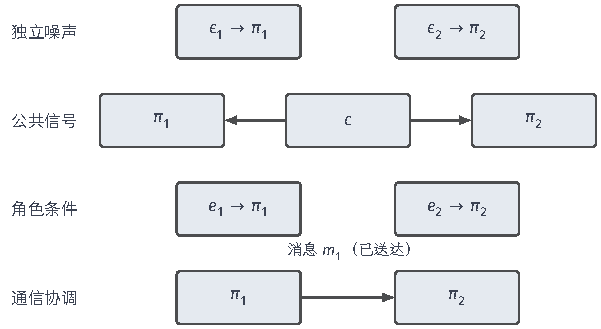
\includegraphics[width=101.741mm]{figures/10-reinforcement-learning/03-task-expansion-and-trustworthiness/tikz/rl-multi-agent-exploration.pdf}
 \caption{联合探索的四种动作与消息生成路径。独立噪声不能保证共同事件发生；公共信号、角色条件和通信分别提供协调依据，箭头表示执行者在动作前实际取得的观测、消息或随机信号。}
 \label{fig:rl-multi-agent-exploration}
\end{figure}

在公共信号例中，真实联合概率$\mathbb P(a_1=\text{按},a_2=\text{按})=0.1$，边缘概率的乘积却是0.01。若将后者作为行为概率，重要性权重就会错十倍。动作依赖通信或同一随机数时也须作同样检查：可以直接保存真实联合概率，也可以先保存使条件独立成立的信号，再计算条件概率的乘积。

% Outline: 7.3.3
\subsection{经验分布变化与目标覆盖检验}
\label{sec:rl-multi-agent-coverage}

取得联合交互记录后，先检查其生成策略、伙伴组成和采集协议是否仍适用于目标。由式\eqref{eq:rl-multi-agent-induced}，版本$k$的对手以$q^{(k)}$概率等待时，自身前进的诱导奖励为$-4+3q^{(k)}$。等待概率改变$\Delta q$，奖励就改变$3\Delta q$，后续状态占用也可能随通过概率变化。不过，版本号变化只是潜在漂移的线索；是否实际发生漂移，应结合分层统计、预测残差或已知策略概率判断。

随后要检查支持，即生成机制是否可能产生目标需要的事件。设日志只以各$1/2$概率生成$(0,0)$和$(1,1)$，非对角联合动作概率为0。每个人的两个动作都出现了，但$(0,1)$和$(1,0)$仍无支持。若两个奖励模型在对角线上都给0，在非对角线上却分别给$10$和$-10$，它们产生的日志分布完全相同，对候选偏离的预测却相反。这个反例表明：没有额外结构假设，边缘覆盖不足以识别未见的联合效果。

表\ref{tab:rl-multi-agent-support}按待估量列出需要检查的支持。实践中还须区分总体概率和样本频率：有限样本未出现某事件，不足以证明其总体概率为零，应连同频率报告不确定性。同样，未检出漂移也不足以证明生成机制恒定。

\begin{table}[htbp]
 \centering
 \begin{tabularx}{\linewidth}{@{}l >{\raggedright\arraybackslash}X >{\raggedright\arraybackslash}X@{}}
 \toprule
 估计对象 & 所需支持 & 典型缺失\\
 \midrule
 目标联合价值 & 目标到达状态及联合动作，目标伙伴 & 某种配合从未采到\\
 最佳响应 & 固定对手下候选完整策略的状态与动作 & 只记录原策略的到达状态\\
 个体反事实优势 & 固定其他动作后的自身候选动作 & 仅含对角动作的记录不能估非对角值\\
 消息条件价值 & 对应消息历史、角色、策略类型 & 未记消息使条件分布不可恢复\\
 \bottomrule
 \end{tabularx}
 \caption{待估量所需的联合支持及常见缺口。增加集中状态输入可以细化条件，却不能提供未发生的联合行为后果。}
 \label{tab:rl-multi-agent-support}
\end{table}

% Outline: 7.3.4
\subsection{覆盖充分时的可用经验构造}
\label{sec:rl-multi-agent-reweight}

目标事件有支持之后，还要处理来源比例与目标不一致的问题。只用最近窗口可缩小版本跨度，代价是丢弃旧版本策略产生的交互记录；按参与者分层可控制伙伴组成；将类型或版本输入价值网络，可分别估计不同对手条件下的后果。若已知生成概率，还可以用重要性校正把行为分布下的期望换为目标分布下的期望。这些措施分别改变样本选择、估计条件或期望测度，可以组合，但没有一种能无条件消除共同学习的非平稳性。

令$k$为一回合抽到的策略群体身份，$\tau$为长度$H$的完整理论轨迹，$q_\beta,q_\pi$分别为行为与目标的伙伴分布。要换算期望，先假设两过程具有相同的初始分布、联合反馈核$K$、环境终止规则和消息送达协议，并且目标联合轨迹分布对行为分布绝对连续，即目标有概率的事件在行为中也有概率。下面的$p_\pi,p_\beta$是相应完整轨迹律的质量函数或共同支配测度下的密度。将轨迹生成概率相除，得到
\begin{equation}
 w(\tau,k)=\frac{p_\pi(\tau,k)}{p_\beta(\tau,k)}
 =\frac{q_\pi(k)}{q_\beta(k)}
   \prod_{t=0}^{H-1}
   \frac{\bm\pi(\bm a_t\mid\bm I_t,k)}
        {\bm\beta(\bm a_t\mid\bm I_t,k)}.
 \label{eq:rl-multi-agent-is}
\end{equation}
两过程相同的联合反馈核项在比值中整体相消；这一步不要求后继状态、奖励、观测与终止反馈在核内独立。留下的是伙伴抽样与逐时刻联合动作的概率比。策略产生的消息若未包含在动作内，还须保留消息概率比；公共信号分布若改变，也须乘上其比值。只有给定记录历史与公共信号后各人条件独立，联合动作比才能分解为$\prod_i\pi_i(a_{i,t}\mid I_{i,t},k)/\beta_i(a_{i,t}\mid I_{i,t},k)$。据此，对完整轨迹函数$f$有$\mathbb E_\pi f=\mathbb E_\beta[wf]$；只估计某个时刻的奖励时，逐决策形式使用截至该奖励的前缀比，不必包含未来动作。

把该权重用于可见记录时，还须能从记录恢复计算概率比所需的动作历史、伙伴身份和消息字段。若$f$与$w$均可由记录计算，完整轨迹上的换测度等式也给出记录上的相应等式；丢弃这些必要字段后，应先边缘化得到记录密度比，不能直接沿用完整轨迹的乘积。

实际构造可以按来源分层取样，恢复真实条件概率，再以所得权重加权回报或损失。按上述个体条件分解计算时，长度$H$的轨迹需要计算$mH$个个体策略概率，还包括伙伴与信号概率。概率比连乘可能带来很大波动：每个个体比值为2时，十人同一步的乘积已经是1024，长轨迹还会继续累积。截断为$\min(w,c)$能限制极端样本影响，但所估期望也改为$\mathbb E_\beta[\min(w,c)f]$，由此产生的偏差必须报告。行为概率为零的事件则没有可加权的样本，不能通过设置无限大权重补回。

另一种处理历史策略回放记录的方法是策略指纹：把训练轮次、探索率等生成条件输入价值网络，使网络区分不同来源。它改变的是估计器读取的训练轮次、探索率等条件变量，不是概率测度，因此不带来重要性校正的无偏结论。多智能体经验回放中已有对两者的直接比较，结果仍限于相应任务和实现条件\scite{rl7-foerster2017replay}

% Outline: 7.3.5
\subsection{覆盖不足时的经验补充与学习边界}
\label{sec:rl-multi-agent-data-boundary}

若检查发现缺口，下一步由访问权限决定。有权继续采集时，可调整伙伴抽样以补充未见参与者，使用合法公共信号或通信探索未见联合动作；缺的是后续状态时，需要改变到达策略，仅在入口加噪声未必有用。若缺的是动作概率、消息等日志字段，应补充后续日志字段，已经丢失的历史通常无法追补。图\ref{fig:rl-multi-agent-data-loop}按访问权限标出哪些缺口可以回到采集环节。

\begin{figure}[htbp]
 \centering
 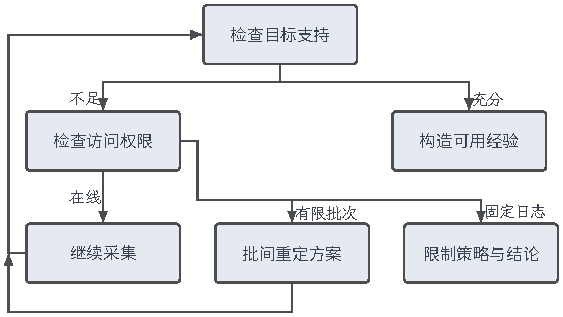
\includegraphics[width=95.282mm]{figures/10-reinforcement-learning/03-task-expansion-and-trustworthiness/tikz/rl-multi-agent-data-loop.pdf}
 \caption{覆盖缺口与记录访问权限决定的处理路径。在线访问允许补采，有限批次只允许批间调整；固定日志不能继续交互，须限制目标或明确引入可检验假设。}
 \label{fig:rl-multi-agent-data-loop}
\end{figure}

有限批次可采用如下协议：总共$B$批，第$b$批包含$N_b$个联合环境步；批内冻结行为策略、伙伴抽样与探索规则，批结束后再按反馈选择第$b+1$批方案。若对手在内部在线适应，须将其适应规则作为策略的一部分声明，并记录所依赖的历史，不能将它称为固定的状态条件对手。只有固定日志时，可将策略限制在有支持的区域、增加可检验结构假设，或按第\ref{chap:rl-information}章采用悲观评价。网络容量再大，也不能从相同日志中区分前述两个奖励模型，因而不能单独解决不可识别性。

% Outline: 7.4
\section{不同参与者依赖下的行为后果估计}
\label{sec:rl-multi-agent-estimation}

联合经验有了明确来源、也确认了覆盖后，估计“某个动作的后果”仍有多种做法，区别在于保留多少参与者之间的依赖。可以把所有人的当前动作都保留下来，估计一个完整的联合价值；也可以固定其他人的动作，只比较我换成别的动作会怎样（个体反事实）；还可以假定联合价值能由各人的局部效用组合而成（局部分解）；或者干脆去预测伙伴会怎么行动，把伙伴的行为显式建进模型；更复杂时，还要计入“我的改变会诱发伙伴如何回应”。这五种估计方式回答不同问题、服务不同计算，可以叠加使用。例如集中训练的评论家可以同时以伙伴类型为条件、又输出固定他人动作后我的全部候选动作价值；群体学习器也可以用单调分解来计算近似的相互响应。

% Outline: 7.4.1
\subsection{基于联合行为的后果估计}
\label{sec:rl-multi-agent-joint-value}

先考虑利用全局状态、联合动作及所需历史的集中评价：固定要评价的联合策略$\bm\pi$，把当前所有人的动作也作为输入，估计一个完整的联合动作价值。做这种集中评价时，评论家用于递推的条件变量$x_t$必须足以预测它会产生的后继过程：完全可观测且策略无记忆时可取$s_t$，策略依赖历史时则要取$(s_t,\bm I_t)$。
\begin{align}
 Q_i^{\bm\pi}(x,\bm a)
 &=\mathbb E[G_{i,t}\mid x_t=x,\bm a_t=\bm a],\\
 V_i^{\bm\pi}(x)
 &=\sum_{\bm a}\bm\pi(\bm a\mid x)Q_i^{\bm\pi}(x,\bm a).
\end{align}
其中$Q_i$评价本次联合动作已确定、随后照$\bm\pi$执行的长期后果，$V_i$还按现有策略平均本次动作。$\bm\pi(\bm a\mid x)$只是在集中条件变量$x$下写出各合法局部策略产生的分布，并未授予行动者读取整个$x$的权限。若现有策略不给某个合法联合动作正概率，其$Q_i$仍可通过从$x$强制执行该动作、随后遵循$\bm\pi$的过程定义；不能用零概率事件上的条件期望唯一确定它。

为从训练样本中的联合转移记录递推这些价值，将回报拆成即时奖励与折扣后的后继回报，再对后继集中条件变量及联合动作取条件平均，得到Bellman评价式
\begin{equation}
 Q_i^{\bm\pi}(x,\bm a)=R_i(x,\bm a)+
 \gamma\sum_{x',d}T_x(x',d\mid x,\bm a)(1-d)
       \sum_{\bm a'}\bm\pi(\bm a'\mid x')Q_i^{\bm\pi}(x',\bm a').
 \label{eq:rl-multi-agent-joint-bellman}
\end{equation}
连续空间中，相应求和改为积分。上式只使用期望的线性分解，没有假设$r_i$、$x'$与$d$条件独立。训练时可用一条完整联合反馈样本替代条件期望，构造
$y_i=r_i+\gamma(1-d)V_{i,\text{目标}}(x')$，再最小化$(Q_{i,\bm\phi}(x,\bm a)-y_i)^2$作TD更新。这里$d$只表示真实终止：终止后没有后继回报，因而乘$1-d$；采样截断但过程未终止时，仍须保留后继价值。日志必须按第\ref{sec:rl-multi-agent-records}节保存或重建与当前接口一致的$x'$。

若要按零和或Nash标准选择后续行为，Minimax-Q将内层策略平均换成零和阶段价值，Nash-Q换成选定均衡的收益。此时进行的是控制备份，而不是对同一个固定$\bm\pi$的评价。即使保留集中训练，也未必需要输入当前联合动作。多智能体深度确定性策略梯度（multi-agent deep deterministic policy gradient, MADDPG）使用动作价值，评价各人的连续动作组合；多智能体PPO（multi-agent PPO, MAPPO）使用状态价值，作为采样回报的比较基准。表\ref{tab:rl-multi-agent-critics}比较这两种评论家接口。

\begin{table}[htbp]
 \centering
 \begin{tabularx}{\linewidth}{@{}l >{\raggedright\arraybackslash}X >{\raggedright\arraybackslash}X@{}}
 \toprule
 方法 & 训练输入与评价对象 & 策略更新与执行\\
 \midrule
 MADDPG & 集中条件变量$x$及$\bm a$；各自$Q_i(x,\bm a)$ & 对自身动作求价值梯度；执行仅用局部输入的确定性行动者\\
 MAPPO & 集中状态或联合观测，可补个体观测或角色标签；$V_i(x)$或团队$V(x)$ & 用回报与$V$构造优势；执行仅用局部输入的随机行动者\\
 \bottomrule
 \end{tabularx}
 \caption{集中动作价值与状态价值的两种接口。联合观测是否足以预测后继过程仍须论证；状态价值评论家不必输入当前联合动作。}
 \label{tab:rl-multi-agent-critics}
\end{table}

MADDPG用集中动作价值指导确定性行动者，可处理合作或竞争收益。MAPPO研究则在合作任务中考察集中状态价值怎样配合PPO，报告的是相应实现条件下的经验表现。两者使用不同评论家，并不意味着集中训练天然优于其他训练权限\scite{rl7-lowe2017,rl7-yu2022}

两种接口都依赖联合轨迹，需承担集中状态与联合历史的传输、价值网络前后向计算和联合轨迹存储成本。这些集中条件变量可帮助区分他人动作的作用，却既不冻结他人策略，也不消除函数逼近误差。尤其当$x$只含当前观测、遗漏对方记忆时，式\eqref{eq:rl-multi-agent-joint-bellman}所需的Markov条件仍可能缺失。训练得到价值之后，行动者还须遵守第\ref{sec:rl-multi-agent-permissions}节的执行权限。

% Outline: 7.4.2
\subsection{基于个体行为反事实的后果估计}
\label{sec:rl-multi-agent-counterfactual}

合作任务里只有一个共同奖励，于是会出现“功劳算谁的”问题：一次成功通过，究竟是因为我主动前进，还是因为对方及时等待？这就是团队中的信用分配。它最干净的形式可以先在一步任务里看清：把入口截成“一次联合动作后立即终止”的独立矩阵任务（故动作价值等于即时奖励），下一小节的表示反例也沿用这一约定。

要量化个人贡献，一种直接的做法是：先规定一个参照动作$c_i$（代表“我本来可以怎么做”），再比较“我实际这么做”和“换成参照、其他人不动”两种情况下的团队奖励之差，称为\term{差分奖励}（difference reward）：
$D_i=R(x,\bm a)-R(x,(c_i,\bm a_{-i}))$。已知上述一步奖励表时，取$c_1=W$得到$D_1=3$。实际交互只执行了一个联合动作，通常没有替代动作的第二份实测结果，而且替代动作还可能改变后继状态。因此，差分的来源须明确为模型、额外试验或价值估计，不能把它作为原日志中已经观察到的事实。

若要指导长期策略更新，需比较候选动作的回报价值，而不只比较即时奖励。反事实多智能体策略梯度（counterfactual multi-agent policy gradients, COMA）用当前策略规定参照：保持其他人的本次动作$\bm a_{-i}$不变，将$i$的候选动作价值按$\pi_i$平均作基线，再与实际动作价值相减：
\begin{align}
 b_i(x,\bm a_{-i})
 &=\sum_{\tilde a_i}\pi_i(\tilde a_i\mid I_i)
       Q^{\bm\pi}(x,(\tilde a_i,\bm a_{-i})),\\
 A_i^{\text{COMA}}(x,\bm a)
 &=Q^{\bm\pi}(x,\bm a)-b_i(x,\bm a_{-i}).
 \label{eq:rl-multi-agent-coma}
\end{align}
例如，1以$1/4$概率前进、$3/4$概率等待且2已等待时，上述一步任务的基线为
$\tfrac14(2)+\tfrac34(-1)=-1/4$，前进的优势为$9/4$。它小于固定以等待为参照的差分3，是因为基线比较当前策略的平均动作，而非固定动作$W$。

依赖别人实际动作的基线，是否会改变策略梯度的期望？先将获准使用的公共信号纳入各$I_i$，并要求给定足以描述联合后继过程的条件变量$x$和其他动作$\bm a_{-i}$后，$i$的条件动作分布仍为$\pi_i(\cdot\mid I_i)$。在策略可微、支持固定且得分与基线的乘积可积时，$b_i(x,\bm a_{-i})$不随本次抽到的$a_i$改变；更新中还须把它视为常数，停止通过基线反向传播。因而可以将它提出动作求和：
\begin{align}
 &\mathbb E_{a_i\mid x,\bm a_{-i}}
   [\nabla_{\bm\theta_i}\log\pi_i(a_i\mid I_i)b_i(x,\bm a_{-i})]\nonumber\\
 &\quad=b_i(x,\bm a_{-i})
       \sum_{a_i}\nabla_{\bm\theta_i}\pi_i(a_i\mid I_i)=0.
 \label{eq:rl-multi-agent-baseline-zero}
\end{align}
最后一步使用概率归一化：$\sum_{a_i}\pi_i(a_i\mid I_i)=1$，对参数求导为零。再平均$(x,\bm a_{-i})$就得到基线项零均值，承接定理\ref{thm:rl-learning-baseline}。若两人共享未记录的随机信号，给定$\bm a_{-i}$后的自身分布可能不再是$\pi_i$，推导中的替换就失效。需要在真实联合策略中处理相关信号，重新推导得分与基线；只将得分改成另一个条件分布的对数梯度，还不足以证明估计的仍是原目标梯度。

为计算该基线，COMA评论家可一次输出自身全部候选动作价值，避免逐个候选运行完整网络。但输出规模仍随$|\mathsf A_i|$增长，连续动作还需近似积分。评论家的训练目标来自联合轨迹，未执行候选的价值仍是估计，而非新增观测。原方法据此将集中评论家与分散行动者连接起来\scite{rl7-foerster2018coma}

零均值结论只保证从精确价值中减去该基线不改变策略梯度期望，并不保证任何基线都降低方差；评论家误差还可能使优势估计失真。此处的“反事实”指固定他人当前动作的候选价值比较，不能据此宣称识别了因果结构模型中唯一真实的个人贡献。

% Outline: 7.4.3
\subsection{基于局部行为组合的后果估计}
\label{sec:rl-multi-agent-factorization}

联合价值回答了“整组动作有多好”，但部署时每个人只能在本地独立选择自己的动作，他既看不到联合价值表、也无法和所有人实时联合优化。于是需要另一种结构：让每个人只计算一个依赖本地历史的局部效用，再保证“每个人都选本地最优”这件事拼起来恰好等于“联合动作最优”。形式地说，设各人只能计算局部效用$q_i(I_i,a_i)$并各自执行$a_i^*\in\arg\max_{a_i}q_i(I_i,a_i)$，所有局部贪心动作能组成联合贪心动作这一性质称为\term{个体与整体最大化一致性}（individual-global-max, IGM）；这里效用是帮助组合团队行为的内部量，不必等于$i$自己的环境回报。

\Needspace{24\baselineskip}
图\ref{fig:rl-multi-agent-mixers}给出两种实现这种一致性的结构。价值分解网络（value decomposition networks, VDN）直接设$Q_{\text{tot}}=\sum_i q_i$，把各人的局部效用相加；单调价值函数分解方法QMIX（monotonic value function factorisation）允许训练状态决定混合器参数，但以非负权重和单调激活保证$\partial Q_{\text{tot}}/\partial q_i\geq0$。提高任一局部效用不会降低联合值，因此部署时可只保留局部贪心选择，无须读取状态。实现这一便利的代价，是分别将联合价值限制为加和或单调组合\scite{rl7-sunehag2018,rl7-rashid2018}

以下充分条件将“不降低联合值”的性质转成对局部贪心动作的保证。

\begin{theorem}[单调组合的局部贪心充分性]
\label{thm:rl-multi-agent-monotone}
固定评论家条件变量$x$及所有局部历史，假设联合动作集合是各人动作集合的笛卡尔积，且局部最大值都存在。若
\[
 Q_{\text{tot}}(x,\bm a)
 =f_x(q_1(I_1,a_1),\ldots,q_m(I_m,a_m))
\]
对每个局部效用逐坐标非减，就有
\[
 \prod_i\arg\max_{a_i}q_i(I_i,a_i)
 \ \subseteq\ \arg\max_{\bm a}Q_{\text{tot}}(x,\bm a).
\]
\end{theorem}
\begin{proof}
任取一组局部最大化动作$\bm a^*$，从任意联合动作$\bm a$开始逐个替换分量。第一分量改为$a_1^*$时，$q_1$不下降，其余效用保持不变；由$f_x$对第一坐标非减，联合值也不下降。第二分量改为$a_2^*$时理由相同，依次完成$m$次替换便有
$Q_{\text{tot}}(x,\bm a)\leq Q_{\text{tot}}(x,\bm a^*)$。由于起点$\bm a$任意，$\bm a^*$最大化联合值；又因为任意局部最大化组合都可作上述替换，故得到所述包含关系。
\end{proof}

保证方向仅从局部最大化指向联合最大化，不能无条件写成等号。例如$f_x$为常数时，全部联合动作都最优，$q_1$却可以只有一个最大化动作；平台区间与并列效用也会造成差别。若合法动作之间存在耦合约束，各人合法动作的乘积可能包含非法组合，逐分量替换就未必保持可行，需重新检验证明条件。

\begin{figure*}[htbp]
 \centering
 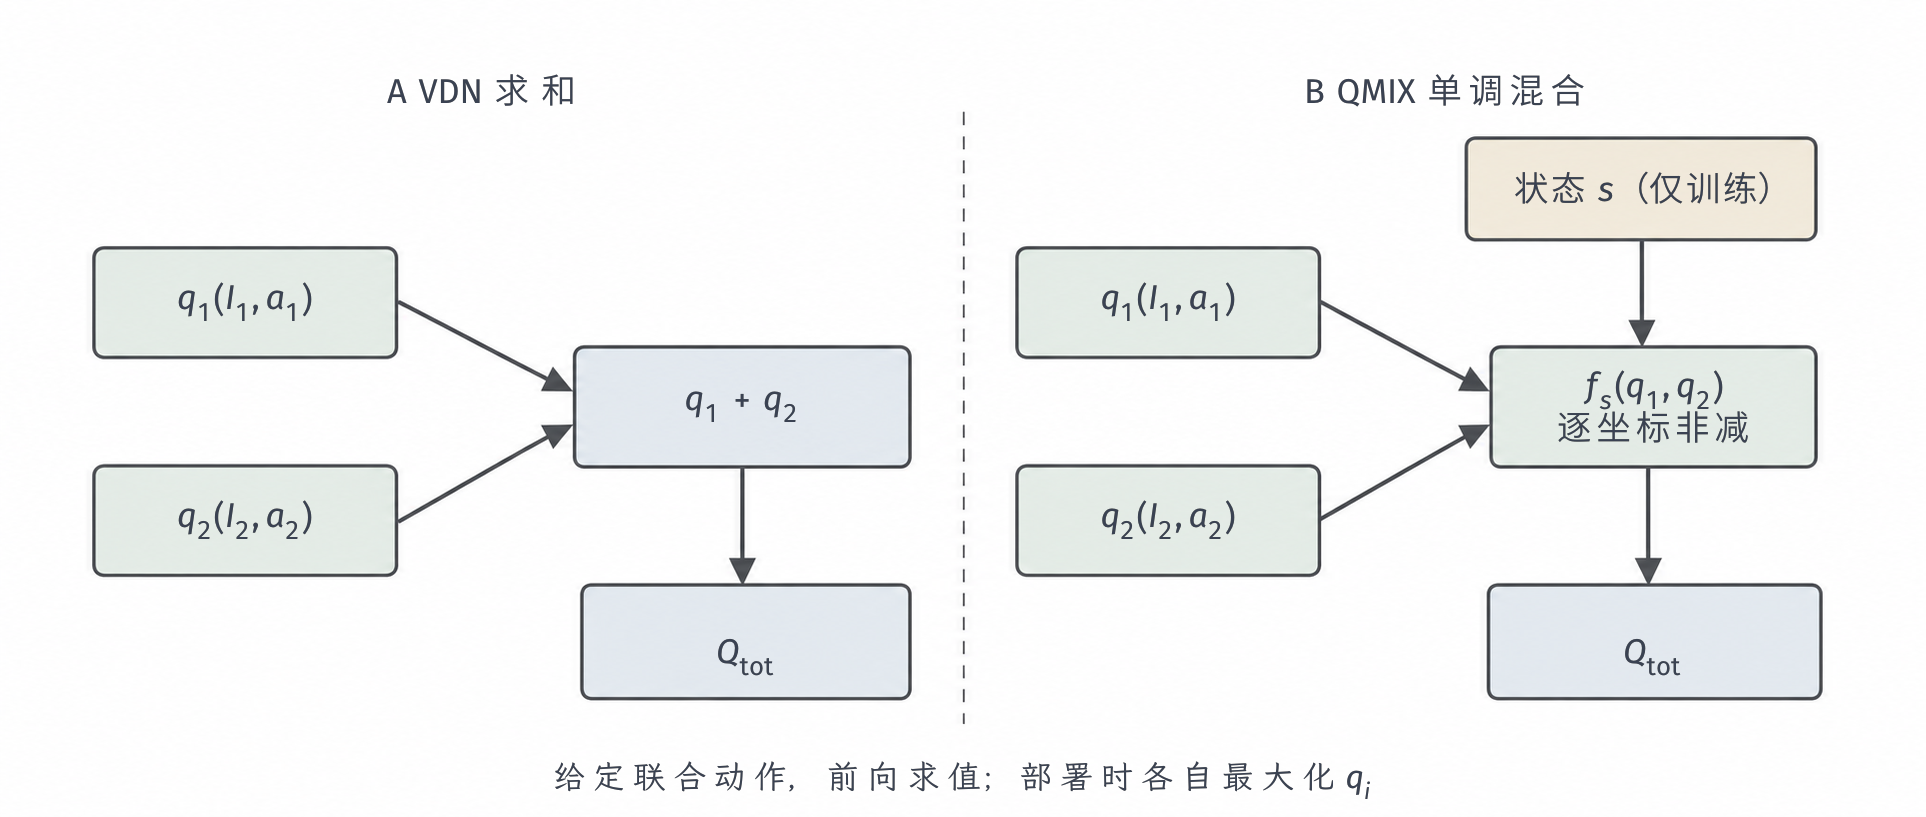
\includegraphics[width=157.400mm]{figures/10-reinforcement-learning/03-task-expansion-and-trustworthiness/generated/rl-multi-agent-mixers/figure.png}
 \caption{给定联合动作时，VDN与QMIX由标量局部效用$q_i(I_i,a_i)$组合联合价值。图中只画前向求值；训练时联合TD损失经求和或单调混合器向全部局部效用网络反传。状态仅供QMIX训练混合器使用，部署时各人选择自身$q_i$的最大化动作。}
 \label{fig:rl-multi-agent-mixers}
\end{figure*}

单调表示的限制也可以在入口一步奖励表中检验。对方前进时，1等待更好；对方等待时，1前进更好，即两列分别要求
$Q(F,F)<Q(W,F)$和$Q(F,W)>Q(W,W)$。若局部排序$q_1(F)>q_1(W)$，第一列违反非减性；若排序相反，第二列违反；若二者相等，单调混合器在两列都不能产生严格差别。因而固定历史下的标量局部效用不能用这一结构精确表示整张表。然而“1前进、2等待”的固定约定仍可分散执行并取得最优奖励。整表可表示、最优动作可执行与训练能找到该动作，是需要分别验证的三件事。

\Needspace{16\baselineskip}
若任务需要更丰富的价值模式，可以放松或改写组合约束，表\ref{tab:rl-multi-agent-factorization}列出两种方式。QTRAN用价值变换和一致性约束保持最优动作；QPLEX以优势分解表示更一般的IGM结构。它们扩大的是表示能力，不是行动者可读取的观测、历史和消息范围。结构在理论上能表示某种值，还须与实际训练是否满足约束、函数逼近误差及优化误差分开判断\scite{rl7-son2019,rl7-wang2021qplex}

\begin{table}[htbp]
 \centering
 \begin{tabularx}{\linewidth}{@{}l >{\raggedright\arraybackslash}X >{\raggedright\arraybackslash}X@{}}
 \toprule
 结构 & 保留的限制或分解 & 代价与边界\\
 \midrule
 VDN & 联合价值为局部效用之和 & 组合便宜；不能表达一般相互作用\\
 QMIX & 状态条件的逐坐标非减混合 & 增加混合器；局部排序不能随他人动作反转\\
 QTRAN & 联合价值与易分解变换在贪心处相等、其他动作满足不等式 & 需拟合联合值并施加约束；近似惩罚不保证精确满足\\
 QPLEX & 局部优势$q_i-\max q_i\leq0$以正权组合，另建联合基准值 & 优势与权重结构增加表达力；表示充分性不等于优化收敛\\
 \bottomrule
 \end{tabularx}
 \caption{局部价值组合的表示限制与代价。更换组合结构不妨碍同时使用伙伴条件化、回放管理或群体训练。}
 \label{tab:rl-multi-agent-factorization}
\end{table}

这些结构都可从联合转移构造团队TD目标，并把损失反传到局部网络。差别在于怎样计算目标中的最大值，以及可以容纳哪些联合价值模式。每人有$A$个动作时，直接枚举需处理$A^m$个组合；局部贪心只比较$mA$个效用，再调用混合器。降低的是动作最大化的计算成本，不能据此断言同样数量的样本足以准确学习所有效用。

% Outline: 7.4.4
\subsection{基于其他参与者策略的行为后果估计}
\label{sec:rl-multi-agent-opponent-model}

前面都假定别人的行为已知，但现实中伙伴的策略通常是隐藏的，只能通过交互去推断。关键的直觉是：即使我当前动作完全相同，不同类型的伙伴也会让后果不同。

要把对伙伴类型的判断写成可更新的概率分布，令伙伴信念$b_t(z)=\mathbb P(z\mid I_{i,t})$，即仅依据获准历史形成的类型分布。自身动作$a_{i,t}$可能改变随后看到的证据$e_{t+1}$，故用$\ell(e_{t+1}\mid I_{i,t},a_{i,t},z)$表示相应似然。若动作只依据已记录历史和独立随机数产生，其选择概率不随候选类型变化，可在贝叶斯归一化时相消。于是用新证据更新信念：
\[
 b_{t+1}(z)=
 \frac{\ell(e_{t+1}\mid I_{i,t},a_{i,t},z)b_t(z)}
      {\sum_{\tilde z}\ell(e_{t+1}\mid I_{i,t},a_{i,t},\tilde z)b_t(\tilde z)}.
\]
此更新要求分母大于0，即至少一个具有正先验概率的类型对所见证据赋予正似然。若动作选择使用了未记录的类型线索，动作概率就不能直接消去。若没有直接观察伙伴动作，似然还须对隐藏动作、状态或消息求和，不能在部署辨识中读取仅供训练的真实动作标签。类型若外生变化，则先通过类型转移核预测，再由证据校正。这里与式\eqref{eq:rl-transfer-belief-update}的贝叶斯步骤相同，变化的是推断对象：从任务条件转为参与者行为。

信念可用于评价候选动作。令$Q_i(I_i,b,a_i,z)$表示固定类型$z$下执行$a_i$，随后按同一套策略及信念更新规则行动的条件回报，则全期望公式给出
$Q_i(I_i,b,a_i)=\sum_z b(z)Q_i(I_i,b,a_i,z)$。
各项都须平均尚未观察的伙伴动作和状态，不能为每个类型偷偷换用“已知类型时”的最优策略，否则平均后不再对应实际可执行行为。后续若继续辨识类型，价值状态与递推也须保留信念更新；把信念冻结的近似会遗漏探测反馈对后续动作选择及回报的影响。

类型模型也可不用有限标签，而用历史编码器输出一个向量，再由该向量预测下一动作的分布。训练时最小化可见动作的负对数似然，即提高模型赋给实际观察动作的概率，学得的表示再输入条件评论家或策略。每次更新需支付历史编码、似然预测及候选动作评价的计算成本，不必直接读取对方网络参数。身份、检查点版本和潜在类型仍不能混为一谈，同一身份可以改用策略，不同身份也可能行为相同。上述估计将对手视为固定或外生变化，尚未计入自身更新诱发的响应。

% Outline: 7.4.5
\subsection{基于参与者相互响应的行为后果估计}
\label{sec:rl-multi-agent-response-model}

比“伙伴类型固定”更进一步的是：伙伴也在学习、会对你的改变作出反应。自身行为改变后，对方可能让步，也可能采用更强硬的规则；只拟合他当前的等待率，就漏掉了“我的策略改变会诱发他如何回应”这一条影响途径。

在两人问题中，固定响应前的对方参数$\bm\psi_0$，以
$\bm\psi'=\mathcal R(\bm\theta_i;\bm\psi_0)$表示对方看到$i$的策略或交互之后采用的参数，$J_{-i}$为对方目标。若$\mathcal R(\bm\theta_i;\bm\psi_0)=\bm\psi_0$，就回到固定对方的估计。若预测对方作一步学习，可规定
$\bm\psi'=\mathcal R(\bm\theta_i;\bm\psi_0)
=\bm\psi_0+\eta\left.\nabla_{\bm\psi}J_{-i}(\bm\theta_i,\bm\psi)\right|_{\bm\psi=\bm\psi_0}$，其中求响应映射对$\bm\theta_i$的导数时保持$\bm\psi_0$固定。这一规则还要求说明它使用的目标、当前策略和用于估计梯度的联合轨迹训练样本。继续增加推理层次时，还须规定对方是否知道$i$的更新规则、是否也预测$i$；增加递归深度会增加假设，而非自动增加准确性。

为区分自身直接改变与对方响应的影响，若$J_i$及$\mathcal R$在所考察邻域可微，可对复合回报使用链式法则：
\begin{equation}
 \nabla_{\bm\theta_i}J_i(\bm\theta_i,\mathcal R(\bm\theta_i;\bm\psi_0))
 =
 \left.\partial_{\bm\theta_i}J_i(\bm\theta_i,\bm\psi)
       \right|_{\bm\psi=\bm\psi'}
 +[D_{\bm\theta_i}\mathcal R(\bm\theta_i;\bm\psi_0)]^\top
 \left.\nabla_{\bm\psi}J_i(\bm\theta_i,\bm\psi)
       \right|_{\bm\psi=\bm\psi'}.
 \label{eq:rl-multi-agent-response-gradient}
\end{equation}
右侧两个回报偏导都在响应后的$(\bm\theta_i,\bm\psi')$处评价：第一项求导时固定$\bm\psi'$，第二项再用响应映射的Jacobian把对方参数变化传回自身参数；$D_{\bm\theta_i}\mathcal R$则在响应前参数$\bm\psi_0$固定时求得。

用一个独立的单步通道变体演示这两条途径。自己以前进概率$p$行动，对方以前进概率$q$行动，给定$p,q$后两人独立随机化；自己前进且对方等待时得1，其余结果得0，一步后终止。因此自身期望回报为$J(p,q)=p(1-q)$。假设对方观察到自己的策略后采用$q(p)=0.8-0.6p$，$p\in[0,1]$；此时$q$始终在$[0.2,0.8]$内。这个响应函数是教学假设，计分也与前面$-1/-4$的通道任务分开。

在内部点$p_0\in(0,1)$，先固定已经响应的$q(p_0)$，直接改变$p$所得导数为$1-q(p_0)=0.2+0.6p_0$。再计入对方前进概率的变化，间接项为$-p_0q'(p_0)=0.6p_0$，两者合计$0.2+1.2p_0$。也可先代入得到$J(p,q(p))=0.2p+0.6p^2$再求导，得到相同结果。若始终把对方固定为$q=0.8$，目标就是$0.2p$，导数才恒为0.2；两种计算对应不同的响应假设。

一步学习响应还需对对方的梯度更新求导，因而涉及梯度的导数；只有交互观测时则要先拟合响应模型，承担相应误差。学习感知的对方学习（learning with opponent-learning awareness, LOLA）据对方学习步骤构造了此类更新\scite{rl7-foerster2018lola}

式\eqref{eq:rl-multi-agent-response-gradient}暂将$\mathcal R$视为确定映射。若它由随机采集的训练样本更新产生，对一份固定样本求导仅得到条件导数；若训练样本的采集律也随$\bm\theta_i$变化，完整期望梯度还包含分布的导数。第\ref{sec:rl-transfer-value-training}节的元学习目标同样区分了固定样本求导与对采样过程求导。

若最佳响应多解或不连续，式\eqref{eq:rl-multi-agent-response-gradient}的可微映射假设可能不成立；对手若不按所设规则学习，求得的导数也只描述错设模型。更深层推理会提高计算成本并放大这种风险。预测下一次响应只是预测任务；斯塔克尔伯格式（Stackelberg）承诺解要求先行者公开承诺策略，后行者据此作最佳响应，因而还须有可承诺、可观察的先后行动协议。同时行动下的Nash均衡又要求固定他人策略后检验单方偏离。三者不能凭响应模型的复杂程度相互替代。

% Outline: 7.5
\section{多智能体的策略更新与学习动态}
\label{sec:rl-multi-agent-learning}

有了价值与优势，还要规定策略如何据此更新，而多智能体的更新比单人多了两个层面的牵连。一个训练批次可以产生价值更新或梯度步；与此同时，各学习者既可以只针对当前对手响应，也可以针对历史上出现过的行为响应；训练对手还可以由一个不断扩充的策略群体来安排配对。例如“从策略库中抽对手，再用策略梯度训练近似最佳响应，最后把新响应加回库”，就同时规定了三件事：更新怎么算（梯度/价值）、相互如何适应（对库中对手）、以及训练群体如何组织（扩充策略库）。下面分别讲清这三个环节，最后再追问：当大家都在同时学习时，这个过程是否稳定、能保证什么。

% Outline: 7.5.1
\subsection{由价值与梯度计算策略更新}
\label{sec:rl-multi-agent-update}

先在本轮计算中冻结其他策略与目标评论家。对训练批次$D_{\mathrm{batch}}$中的联合转移求后继目标，再拟合价值或构造优势，最后得到新动作规则或新策略参数。表\ref{tab:rl-multi-agent-value-updates}按这条路径比较几种价值方法。独立Q学习把他人行为边缘化，只有条件变量足以预测诱导后继过程、诱导环境平稳等前提成立，才能援引表格型单智能体Q学习保证；共同更新、压缩局部历史或使用函数逼近，都可能破坏这些前提。

\begin{table}[htbp]
 \centering
 \begin{tabularx}{\linewidth}{@{}l >{\raggedright\arraybackslash}X >{\raggedright\arraybackslash}X >{\raggedright\arraybackslash}X@{}}
 \toprule
 方法 & 价值输入 & 后继备份 & 动作与执行时可读变量\\
 \midrule
 独立Q & $I_i,a_i$ & 自身$\max Q_i$ & 局部贪心；他人行为被边缘化\\
 Minimax-Q & $s,\bm a$ & 零和矩阵价值 & 按解出的混合策略抽样；需状态\\
 Nash-Q & $s,\bm a$的各人收益 & 选定阶段均衡收益 & 按同一均衡选择约定；需状态\\
 VDN & 局部$I_i,a_i$再求和 & 局部最大值之和 & 每人局部贪心\\
 QMIX & 局部效用与训练状态 & 单调混合的局部最大值 & 每人局部贪心；执行无须状态\\
 \bottomrule
 \end{tabularx}
 \caption{由价值目标生成动作的不同接口。各行仍需规定联合采样、终止处理和目标网络；即使算出了阶段博弈解，也须检查执行所需的状态、观测或公共建议是否可读。}
 \label{tab:rl-multi-agent-value-updates}
\end{table}

一条教学样本即可显示参数化怎样影响更新。设通道样本奖励$r=2$，尚未终止，目标网络给后继联合值1，$\gamma=0.9$，则目标$y=2.9$。当前$Q=1$时，对$\tfrac12(Q-y)^2$作步长0.1的表格梯度下降，残差$-1.9$使新值为$Q'=1.19$。若改用VDN且两个局部效用为0.4和0.6，同一残差分别传到两个表项，一次同步更新后为0.59和0.79，联合值为1.38。联合值的变化不同，是因为两个参数同时改变了有效步长。QMIX传回残差时还须乘混合器对各效用的导数；Minimax-Q与Nash-Q则须为后继目标运行阶段求解器。

随机行动者也可直接沿收益梯度更新。令$\bm\pi_{\bm\theta}=\prod_i\pi_{\bm\theta_i}(a_i\mid I_i)$，暂不共享参数，并固定其他参数与环境机制。假设策略可微、支持固定，同时满足式\eqref{eq:rl-learning-policy-gradient}所需的可积支配条件，以便交换求导与折扣求和。对轨迹概率取对数后，只有$i$的动作项依赖$\bm\theta_i$；每次动作的得分只需乘其后回报，先前奖励对应的得分期望为零。将未来奖励归并为$G_{i,t}$，再用折扣占用表示时刻求和，得到
\begin{align}
 \nabla_{\bm\theta_i}J_i(\bm\pi)
 &=\sum_{t\geq0}\gamma^t
   \mathbb E_{\bm\pi}
   [\nabla_{\bm\theta_i}\log\pi_i(a_{i,t}\mid I_{i,t})G_{i,t}]
 \nonumber\\
 &=\frac{1}{1-\gamma}
   \mathbb E_{x,\bm a\sim d^{\bm\pi}}
   [\nabla_{\bm\theta_i}\log\pi_i(a_i\mid I_i)
           Q_i^{\bm\pi}(x,\bm a)].
 \label{eq:rl-multi-agent-policy-gradient}
\end{align}
这里$d^{\bm\pi}$是集中条件变量$x$与联合动作上的归一化折扣占用度量，它包含归一化因子$1-\gamma$；目标$J_i$未归一化，故第二行须保留$1/(1-\gamma)$。减去符合条件的基线可将$Q_i$换成优势。若联合策略相关，则要从真实联合概率重新推导得分，并检查第\ref{sec:rl-multi-agent-counterfactual}节的基线条件，不能直接使用各人边缘策略的得分。

此梯度把行动者局部历史与评论家集中条件变量的两种用途分开：行动者以自身局部历史计算动作得分，集中评论家提供该动作的长期后果估计。在一步终止的入口教学样本中，若前进概率$p=1/4$由logit参数生成，即以$p/(1-p)$的对数表示参数，采到$(F,W)$并采用前节精确优势$9/4$，得分为$1-p=3/4$，乘积为$27/16$。步长0.1使logit由$\log(1/3)$增至$\log(1/3)+27/160$，前进概率约为0.283。这里直接更新有限一步样本，没有使用归一化折扣占用，因此不额外乘其系数。

\Needspace{7\baselineskip}
PPO类更新用旧策略产生批次，计算自身动作的概率比$\zeta_{i,t}=\pi_i(a_{i,t}\mid I_{i,t})/
\pi_i^{\text{旧}}(a_{i,t}\mid I_{i,t})$，再最大化以下裁剪代理目标的批次均值：
\[
 \min\{\zeta_{i,t}\widehat A_{i,t},
       \operatorname{clip}(\zeta_{i,t},1-\epsilon,1+\epsilon)
                      \widehat A_{i,t}\}.
\]
其中$\widehat A_{i,t}$为优势估计，$0<\epsilon<1$规定围绕概率比1的裁剪宽度；取两项较小值，限制概率比在有利方向上继续扩大代理目标。独立PPO以局部价值估计优势，MAPPO则用集中状态价值。这里的自身概率比没有包含其他动作和后续轨迹，不能等同于完整联合轨迹的重要性比。同批次反复更新所有人时，对手与状态分布均可能变化，所以裁剪机制本身不构成共同学习的单调改进证明。

对连续可微动作，确定性行动者$a_i=f_{\bm\theta_i}(I_i)$可直接对动作价值使用链式法则。精确同策略梯度中的局部方向为
$\nabla_{\bm\theta_i}f_{\bm\theta_i}(I_i)\nabla_{a_i}Q_i^{\bm f}(x,\bm a)$，以归一化$d^{\bm f}$表示时同样带$1/(1-\gamma)$。MADDPG用目标行动者生成后继动作，由联合回放的TD损失拟合$Q_i$，再估计这一方向；用回放分布替代$d^{\bm f}$得到的是离策略代理更新，未经校正不能称为原$J_i$的无偏梯度。COMA保留随机行动者，采用式\eqref{eq:rl-multi-agent-coma}的优势。表\ref{tab:rl-multi-agent-policy-updates}按计算与采样条件比较这些接口。

\begin{table}[htbp]
 \centering
 \begin{tabularx}{\linewidth}{@{}l >{\raggedright\arraybackslash}X >{\raggedright\arraybackslash}X@{}}
 \toprule
 方法 & 价值、采样与策略方向 & 主要成本或失效处\\
 \midrule
 独立PPO & 近期联合轨迹中的局部$V_i$与裁剪得分梯度 & 价值未以其他人的动作或历史为条件；同时更新漂移\\
 MADDPG & 联合回放$Q_i$与确定性动作梯度 & 集中动作输入、回放失配、评论家动作梯度误差\\
 MAPPO & 近期轨迹中的集中$V_i$与裁剪得分梯度 & 集中状态传输、优势误差、批内复用漂移\\
 COMA & 联合$Q$与固定其他动作的候选基线 & 枚举自身候选；未见动作价值估错\\
 \bottomrule
 \end{tabularx}
 \caption{策略梯度接口的价值、采样和成本差异。梯度所针对的$J_i$由收益设定决定，不能由方法名称推断合作或竞争目标。}
 \label{tab:rl-multi-agent-policy-updates}
\end{table}

这些更新只沿图\ref{fig:rl-multi-agent-ctde}的训练梯度路径传递，部署动作仍由各人的局部决策历史及获准消息生成。团队若共享参数$\bm\theta$，每个人的动作概率都依赖它，轨迹得分便为$\sum_i\nabla_{\bm\theta}\log\pi_{\bm\theta}(a_i\mid I_i)$，用于汇总共同$J$的梯度。若各人$J_i$不同而参数仍共享，就须另定加权目标或更新调度。直接平均冲突梯度也已选择了收益取舍，不能视为不改变目标的实现细节。

% Outline: 7.5.2
\subsection{多个学习者之间的相互适应}
\label{sec:rl-multi-agent-mutual-learning}

即使每个学习者各自的更新方向都确定无误，多人一起更新时的“时序安排”仍会显著改变学习轨迹，因为每个人面对的对手都是一个移动目标。这里有一个带点反直觉、但在零和学习中很关键的现象：两个人各自针对“旧的对方”做改进，并不保证他们合起来在向均衡靠近——双方同时迈一步，可能只是在均衡点周围旋转甚至越转越远。下面用最简单的匹配硬币博弈把这种差别算清楚。记$p,q$分别为第一人、第二人选择其第一个动作的概率。
\[
 p^{(k+1)}=[p^{(k)}+\eta(4q^{(k)}-2)]_{[0,1]},\qquad
 q^{(k+1)}=[q^{(k)}-\eta(4p^{(k)}-2)]_{[0,1]}.
\]
若改为交替更新，先计算$p^{(k+1)}$，第二式就使用这一新值而非$p^{(k)}$。图\ref{fig:rl-multi-agent-trajectories}以同一$\eta=0.1$和初值$(0.7,0.5)$迭代两种规则；第三条历史响应曲线则对截至上轮的平均对手求精确最佳响应，平局时选$1/2$。这样可以在同一博弈中区分更新时序和响应对象的影响。

\begin{figure*}[htbp]
 \centering
 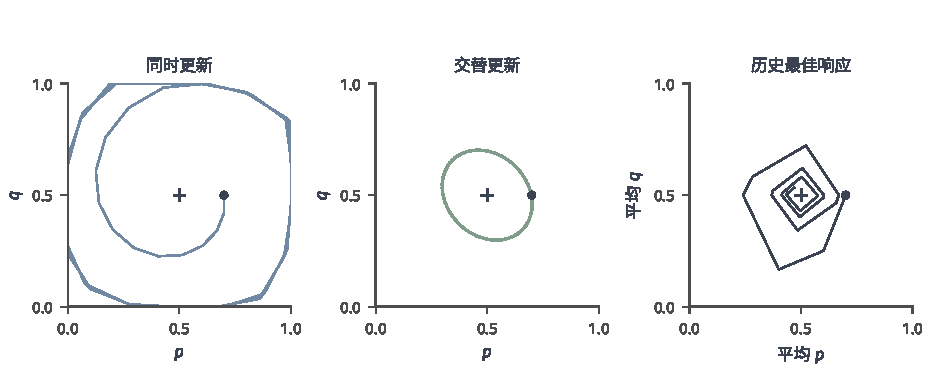
\includegraphics[width=157.400mm]{figures/10-reinforcement-learning/03-task-expansion-and-trustworthiness/matplotlib/rl-multi-agent-trajectories.pdf}
 \caption{匹配硬币博弈中三种响应规则的120次更新。曲线由图源递推式计算，并非实验成绩；圆点标初值，十字标均衡$(1/2,1/2)$，历史响应面板显示累计平均策略。}
 \label{fig:rl-multi-agent-trajectories}
\end{figure*}

在尚未触及投影边界时，令$x=p-1/2,y=q-1/2$表示相对均衡的偏移。同时更新满足
$(x')^2+(y')^2=(1+16\eta^2)(x^2+y^2)$，所以非零偏移在旋转之外还会增大。两人各自针对旧对方改进，并不意味着共同接近均衡。历史响应转而比较整个过去的对手分布，它要减少长期错失的收益，而非只击败最新版本。

要判断这种相互适应长期看是否有效，需要一个比较基准：把自己实际拿到的总收益，与“假如从头到尾固定采用某个动作”能拿到的总收益相比。这个“错失的收益”就是累计外部遗憾，它衡量规则在长期中是否留下了可被持续利用的弱点。
\begin{equation}
 R_i^{(n)}
 =\max_{b_i}\sum_{k=1}^{n}
   [u_i(b_i,\bm a_{-i}^{(k)})
        -u_i(\bm a^{(k)})].
 \label{eq:rl-multi-agent-external-regret}
\end{equation}
最大化在轮次求和之外，意味着$b_i$在所有轮次保持不变。若每轮先取最佳响应再相加，允许替代行为逐轮改变，得到更强的动态比较而非同一遗憾。混合策略版本则用每轮期望收益代替实际动作收益。

用累计遗憾可以直接构造一条很直观的适应规则：过去哪个动作让我错失的收益越多，下一轮就给它越大的选择概率。以$R_i^{(n)}(a)$保存每个固定动作的累计遗憾，记正部为$[r]_+=\max(r,0)$。\term{遗憾匹配}（regret matching）
\[
 \pi_i^{(n+1)}(a)=
 \begin{cases}
 [R_i^{(n)}(a)]_+/\sum_b[R_i^{(n)}(b)]_+,
       &\sum_b[R_i^{(n)}(b)]_+>0,\\
 1/|\mathsf A_i|,&\text{否则}.
 \end{cases}
\]
累计动作遗憾为$(3,-1,1)$时，正部和为4，新分布为$(3/4,0,1/4)$；全非正时，采用均匀回退。上述计算需要所有候选动作的收益，属于已知全部动作收益的更新。已知矩阵可查表，只有实际动作奖励时则需要探索和适当估计，不能将未观测收益直接填入。遗憾驱动的适应规则源于相关均衡学习的工作，第\ref{sec:rl-multi-agent-deviations}节将进一步区分外部与内部偏离保证\scite{rl7-hart2000}

遗憾匹配是在“整个策略”层面比较的；但在序贯博弈（比如前面的隐藏牌游戏）里，完整策略的数量会随决策节点指数增长，逐一比较成本过高。能不能改成在每个信息集局部地评价动作、再把这些局部改进汇总成完整策略的收益？这里有一个关键细节：我自己旧策略很少到达某个节点，不代表“假如我改道去那里”后也很少到达——为了评估改走这条路线的价值，计算局部量时要先把我自己先前的到达概率去掉。

要特别区分这里的“反事实”和前文出现过的两种用法：第\ref{chap:rl-planning}章的规划查询$T(\cdot\mid s,a)$，是在固定规律下预测候选动作的分布；COMA 固定他人当前动作，按自身策略对候选价值取平均作为优势基线；接下来的\term{反事实遗憾最小化}（counterfactual regret minimization, CFR）则保留对方与机会的先前到达概率、只去掉自身先前的到达因子，用局部动作的遗憾来控制完整策略的遗憾。

在图\ref{fig:rl-multi-agent-card-tree}中，将到达历史$h$的概率拆成两部分：$\rho_i^{\bm\pi}(h)$仅乘$i$先前动作的概率，$\rho_{-i}^{\bm\pi}(h)$乘其他人和机会的概率。记终局历史集合为$\mathcal Z$，在$h$强制选$a$、随后按原策略到达$z$的概率为$P^{\bm\pi}(z\mid ha)$，非后继终局取0。先平均后续终局收益，再按对方与机会的到达概率汇总同一信息集中的历史，得到未归一化反事实动作价值：
\begin{align}
 v_i^{\bm\pi}(I,a)
 &=\sum_{h\in I}\rho_{-i}^{\bm\pi}(h)
         \sum_{z\in\mathcal Z}P^{\bm\pi}(z\mid ha)u_i(z),\\
 v_i^{\bm\pi}(I)&=\sum_a\pi_i(a\mid I)v_i^{\bm\pi}(I,a).
 \label{eq:rl-multi-agent-cfr-value}
\end{align}
该式既不乘自身先前到达因子，也不除以$\sum_{h\in I}\rho_{-i}(h)$。它保留的是对方与机会的权重，不是“已到达$I$”之后归一化的普通条件期望。这样的权重将在遗憾分解中与偏离策略的自身到达因子配合，恢复完整策略的收益差。

例如，假定各动作原本均匀，1持$H$、先过牌$K$、2再下注$B$的末级信息集记为$HKB$，其真实到达概率为
$\tfrac12\cdot\tfrac12\cdot\tfrac12=1/8$，反事实权重却为
$\tfrac12\cdot\tfrac12=1/4$，其中删去的是1自身过牌的概率。这样即使1当前很少过牌，仍能比较来到此处后的跟注与弃牌。图\ref{fig:rl-multi-agent-cfr-reach}分开标出这些因子；去掉前序到达因子不同于COMA平均当前自身动作。

\begin{figure}[htbp]
 \centering
 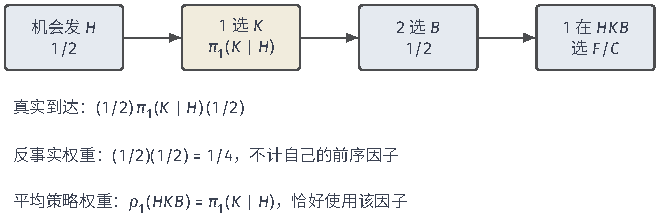
\includegraphics[width=111.651mm]{figures/10-reinforcement-learning/03-task-expansion-and-trustworthiness/tikz/rl-multi-agent-cfr-reach.pdf}
 \caption{高牌信息集$HKB$的真实与反事实到达权重。CFR价值保留机会和2的因子，去掉1的前序选择；用于汇总平均行为策略时，则需要1自身的前序因子。}
 \label{fig:rl-multi-agent-cfr-reach}
\end{figure}

CFR用这些价值在每个信息集运行局部遗憾匹配。一轮完整遍历先冻结$\bm\pi^{(k)}$，从根到叶计算到达因子，再从叶到根汇总式\eqref{eq:rl-multi-agent-cfr-value}。每个动作相对当前局部策略的价值差累加为
\[
 R_i^{(k)}(I,a)=R_i^{(k-1)}(I,a)+
        v_i^{\bm\pi^{(k)}}(I,a)-v_i^{\bm\pi^{(k)}}(I).
\]
遍历结束后，保存当前策略的平均权重，并统一由累计遗憾生成下一轮局部策略，避免同一次遍历混用新旧版本。

表\ref{tab:rl-multi-agent-cfr-round}以零遗憾和全部均匀策略开始，对隐藏牌游戏完成一轮上述计算。原策略期望收益为$J_1=1/8$，表中遗憾与概率均按各行所列动作顺序排列。

\begin{table}[htbp]
 \centering
 \begin{tabular}{@{}llll@{}}
 \toprule
 行动者与信息集 & 动作 & 本轮反事实遗憾 & 下一轮分布\\
 \midrule
 1，持$H$首次行动 & $(B,K)$ & $(3/16,-3/16)$ & $(1,0)$\\
 1，持$L$首次行动 & $(B,K)$ & $(3/16,-3/16)$ & $(1,0)$\\
 1，$HKB$ & $(F,C)$ & $(-3/8,3/8)$ & $(0,1)$\\
 1，$LKB$ & $(F,C)$ & $(1/8,-1/8)$ & $(1,0)$\\
 2，面对$B$ & $(F,C)$ & $(-1/4,1/4)$ & $(0,1)$\\
 2，面对$K$ & $(K,B)$ & $(-1/8,1/8)$ & $(0,1)$\\
 \bottomrule
 \end{tabular}
 \caption{隐藏牌游戏中全树遍历、同步更新的一轮CFR计算。2按自身收益$u_2=-u_1$计算遗憾，故不能直接复用1的收益符号。}
 \label{tab:rl-multi-agent-cfr-round}
\end{table}

以表中$HKB$这一行的计算为例，将终局收益乘上反事实权重，得$v_1(F)=-1/4$、$v_1(C)=1/2$；当前均匀策略值$v_1=1/8$，相减便得$(-3/8,3/8)$。2面对$B$时，高低牌各带对方与机会权重$1/4$，弃牌值为$-1/2$，跟注值为0，均匀当前值为$-1/4$，故只有跟注有正遗憾，下一轮必跟注。其余各行也可由已给的终局收益按同样步骤复算，无须补充游戏规则。

局部遗憾的用途不仅是改变信息集动作。在有限且完全回忆的博弈中，令$\mathcal I_i$为参与者$i$行动的信息集集合，这些局部量还给出完整策略偏离的上界：
\begin{equation}
 R_i^{(n)}
 \leq\sum_{I\in\mathcal I_i}
        \left[\max_a R_i^{(n)}(I,a)\right]_+,
 \label{eq:rl-multi-agent-cfr-bound}
\end{equation}
先用没有对手的两层树看清局部差额怎样相加。根节点选择Stop得到0，选择Go后再选Left或Right，收益分别为2和4。当前策略以$1/2$概率Go，到达下层后又以各$1/2$概率选Left或Right，故旧值为
\[
  \frac12\left(\frac12\,2+\frac12\,4\right)=1.5.
\]
考虑始终Go、随后始终Right的完整偏离，其收益为4。先只改根节点为Go、下层仍按旧策略，收益从1.5提高到3，增益为1.5；再把下层改为Right，收益从3提高到4，增益为1。两个差额相加得到
\[
  (3-1.5)+(4-3)=4-1.5=2.5.
\]
中间的3被消去，留下完整偏离的新旧收益差。下层增益按偏离策略到达下层的概率1计权，而不是按旧策略的到达概率$1/2$计权；否则会漏掉偏离后新增的访问。在博弈中还须保留对方与机会的到达权重，反事实价值正是先保存这部分，再与偏离者自身的到达因子配合。

式\eqref{eq:rl-multi-agent-cfr-bound}的左侧将式\eqref{eq:rl-multi-agent-external-regret}中的固定替代动作扩展为固定完整策略。完全回忆保证同一信息集具有相同的自身前序行动；递归分解收益差时，可以把固定偏离策略的自身到达因子提出信息集历史的求和。该因子介于0和1之间，累计局部增益因而由各信息集最大累计遗憾的正部控制。有限个信息集各自的遗憾增长为$o(n)$时，完整策略遗憾也为$o(n)$。这一结论只支持声明的完整策略偏离类，不能只凭局部观察到的动作收益就假定已取得所有信息集的反事实价值。原始CFR给出了该分解与局部遗憾界\scite{rl7-zinkevich2007}

获得这些局部量仍有成本。全树遍历的每轮计算随访问节点数增长，至少要保存$\sum_I|\mathsf A(I)|$个遗憾项及平均策略累加量。采样CFR可减少单轮访问节点，但需另给采样概率、支持条件，以及无偏反事实估计或相应误差界。任意舍弃罕见分支不能继承全遍历保证，深度近似也会引入拟合误差。

将遗憾界转为均衡保证时，要输出适当的平均策略，而非直接输出最后一轮。在完全回忆下，任取$h\in I$都具有相同的自身前序概率乘积，记为$\rho_i^{(k)}(I)$，不应在信息集内重复累加这一因子。按自身到达概率加权局部动作，得到平均行为策略
\begin{equation}
 \bar\pi_i^{(n)}(a\mid I)=
 \frac{\sum_{k=1}^{n}\rho_i^{(k)}(I)\pi_i^{(k)}(a\mid I)}
      {\sum_{k=1}^{n}\rho_i^{(k)}(I)}.
 \label{eq:rl-multi-agent-average-behavior}
\end{equation}
该比值来自自身序列实现概率的平均：分子对应到达$I$并选$a$的累加概率，分母对应到达$I$的累加概率，二者同时除以轮数后比值不变。逐层应用可恢复均匀抽取整套历史策略时的自身序列概率，而简单逐信息集算术平均通常不能。分母若为零，该信息集在平均实现计划中不可达，可规定任意合法分布，例如均匀分布。

例如，两个版本先过牌概率为0.1和0.9，在$HKB$处跟注概率为1和0。按自身到达加权的平均跟注率为0.1，而非算术平均0.5；它使“过牌再跟注”的自身序列概率为$0.5(0.1)=0.05$，正好等于$\tfrac12(0.1\cdot1+0.9\cdot0)$。若两人零和且各自平均外部遗憾至多$\varepsilon$，这些平均策略的总偏离间隙至多$2\varepsilon$，各人的偏离收益因此也至多$2\varepsilon$。第\ref{sec:rl-multi-agent-deviations}节将用零和消去证明这一结论；它不要求当前策略收敛，也不提供一般和Nash保证。

% Outline: 7.5.3
\Needspace{24\baselineskip}
\subsection{自我对弈与策略群体的迭代组织}
\label{sec:rl-multi-agent-population}

要让“针对历史响应”的学习真正发生，还得有一套训练对手的组织方式，否则很容易在几代之间丢掉重要的检验。比如一个“总让行”策略会被“总前进”克制；可若下一代只针对“总前进”训练、又把“总让行”彻底丢掉，就再也发现不了对手重新变温和时的机会——策略之间常常存在这种循环相克。

把“保留一批历史策略、再针对它们训练新策略”形式化，就得到策略库式的外循环。\term{策略空间响应预言机}（policy-space response oracles, PSRO）用策略库和库上博弈组织这一外循环。
令参与者$i$保存非空有限策略库$\mathcal P_i=\{\pi_i^1,\ldots,\pi_i^{K_i}\}$，其中$K_i\geq1$，每条策略均遵守原任务的观测、消息与行动权限。索引$k_i\in\{1,\ldots,K_i\}$指定一套完整策略。固定初态与交互协议后，库上收益表定义为
\[
 U_i(k_1,\ldots,k_m)
 =J_i(\pi_1^{k_1},\ldots,\pi_m^{k_m}).
\]
它是该组合的期望回报；由有限次对局估计得到的表另记$\widehat U_i$，并保存对局数、伙伴配对及采样随机性。因而估计误差和库中未包含的策略是两种不同限制。元混合策略$\sigma_i$是库索引上的概率分布，决定本回合使用哪套策略；它不同于环境中的$\pi_i(a_i\mid I_i)$，后者决定给定局部历史时采取哪个动作。通常先为一回合抽取一次索引，再执行整套行为策略，不在每一步重新换网络。

图\ref{fig:rl-multi-agent-psro}将库更新展开。先固定元对手$\bm\sigma_{-i}$，响应训练器对该索引分布平均回报，并优化
\[
 \mathbb E_{\bm k_{-i}\sim\bm\sigma_{-i}}
       J_i(\pi_i,\bm\pi_{-i}^{\bm k_{-i}}).
\]
响应器可调用第\ref{sec:rl-multi-agent-update}节的梯度或价值更新；元策略则可由零和求解器、遗憾更新或其他已规定的群体选择规则产生。获得$\hat\pi_i$后，估计其新增收益表项，将它加入库，再重新求元策略。原始PSRO组合的是近似响应训练与经验博弈求解，外循环并不要求响应器采用唯一的底层算法\scite{rl7-lanctot2017}

\Needspace{28\baselineskip}
实际系统未必完整计算上述元博弈，而会按任务选择群体维护方式。与第\ref{sec:rl-multi-agent-collection-plan}节的OpenAI Five版本抽样相比，AlphaStar的联赛训练（league training）设置主学习者和专门寻找其弱点的不同对手角色，再从保留的历史策略中选择训练对手\scite{rl7-vinyals2019}

OpenAI Five则主要维护共同训练的队伍，并混入历史版本对局以减少遗忘，并非为每个队员建立独立的均衡策略库。两种组织分别侧重多角色查找弱点和主训练中的历史检验。增加角色与库策略需要更多对局、存储和维护；这些机制安排了底层强化学习的经验来源，但系统规模本身不能证明已覆盖完整最佳响应。

\begin{figure}[htbp]
 \centering
 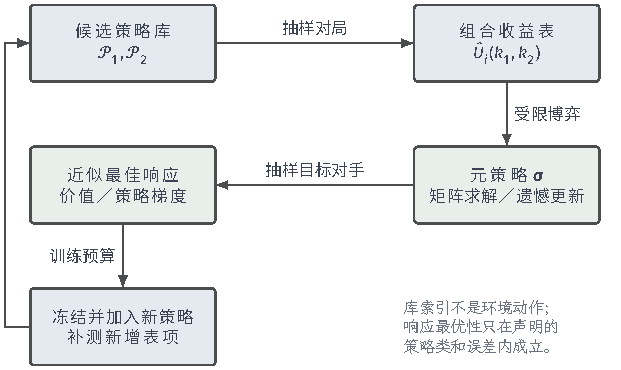
\includegraphics[width=105.184mm]{figures/10-reinforcement-learning/03-task-expansion-and-trustworthiness/tikz/rl-multi-agent-psro.pdf}
 \caption{PSRO的策略库外循环。收益表估计使用对局预算，响应训练使用交互与梯度预算；元策略规定响应对象，响应器规定底层更新计算。}
 \label{fig:rl-multi-agent-psro}
\end{figure}

策略库的限制可由三套抽象教学策略$\alpha,\beta,\chi$说明。以第一人的策略为行、第二人的策略为列，两人的索引都按$\alpha,\beta,\chi$排列，第一人的零和收益表为
\[
 \bm U=
 \begin{pmatrix}0&-1&1\\1&0&-1\\-1&1&0\end{pmatrix}.
\]
从表中可见，$\beta$必胜$\alpha$，$\chi$又必胜$\beta$，没有一套最强纯策略。若双方库只有$\{\alpha,\beta\}$，元解都选$\beta$，库内没有获利偏离；库外的$\chi$却能取得1。加入全部三套策略后，均匀混合使各行收益都为0。这区分了击败当前对手、求解已有收益表中的均衡和覆盖所有可能响应：前两项成立，第三项仍可能失败。

若双方库各有$K$套策略，每格评价$E$局，完整收益表就需$K^2E$场；增加一行一列还须补测相关组合，多方全组合表的项数则为$\prod_iK_i$。响应网络、检查点及响应训练与收益估计的对局记录也占用预算。收益估计误差、响应搜索误差及库外策略都会使元博弈与完整博弈不同，因而受限元解不能单独认证完整博弈不可利用。

% Outline: 7.5.4
\subsection{学习动态的稳定性与保证对象}
\label{sec:rl-multi-agent-stability}

更新怎么算、对谁响应、训练群体如何组织，三者合起来决定了学习动态，因此任何“会收敛/很稳定”的声明都必须对应这一完整组合，换掉其中一个模块结论就可能失效——例如把精确的表格遗憾更新换成误差不受控的神经网络近似，原来的收敛定理就不再适用。表\ref{tab:rl-multi-agent-dynamics}列出各组合实际能保证的输出对象。

\begin{table*}[htbp]
 \centering
 \begin{tabularx}{\linewidth}{@{}l l l >{\raggedright\arraybackslash}X >{\raggedright\arraybackslash}X >{\raggedright\arraybackslash}X@{}}
 \toprule
 更新接口 & 响应规则 & 训练群体 & 当前策略表现 & 平均策略表现 & 保证条件\\
 \midrule
 梯度 & 同时追随 & 当前双方 & 可旋转或发散 & 局部改进不足以保证平均间隙下降 & 另需步长、博弈与算子条件\\
 精确响应 & 历史平均 & 历史策略 & 可持续变化 & 有限两人零和的经典虚构博弈平均可收敛 & 精确响应、完整有限博弈；近似误差另计\\
 局部遗憾 & 同步CFR & 当前与平均 & 不要求收敛 & 适当平均的零和间隙受遗憾界控制 & 有限、完全回忆、正确价值或采样误差控制\\
 梯度响应器 & 元策略响应 & PSRO策略库 & 新响应未必稳健 & 元混合只解受限经验博弈 & 收益表误差、响应误差及策略类限制均需报告\\
 \bottomrule
 \end{tabularx}
 \caption{更新计算、响应规则和群体组织共同确定的保证。当前策略、平均行为策略与库上的元混合策略对应不同输出，应分别报告。}
 \label{tab:rl-multi-agent-dynamics}
\end{table*}

为直观区分这些输出，图\ref{fig:rl-multi-agent-stability}沿用匹配硬币和同一初值，计算交替更新轨迹。固定当前$(p,q)$，两人分别求最佳响应得到总单方偏离间隙
$g(p,q)=|2p-1|+|2q-1|$；检验平均策略时，则代入历轮$p,q$的均值。图中另按固定动作在整段历史上的错失收益计算
\[
 \frac1n\max\!\left\{0,\
 \left|\sum_k(2q^{(k)}-1)\right|-\sum_k u^{(k)},\
 \left|\sum_k(2p^{(k)}-1)\right|+\sum_k u^{(k)}\right\},
\]
这是两人累计平均外部遗憾正部中的较大值，其中绝对值来自比较两个固定纯动作。三条曲线使用同一序列，当前间隙波动时，平均间隙仍可下降。有限步长下遗憾还可能保留偏差，因此图形只能展示所给递推的有限轮次结果，不能据形状断言任意精度收敛。

\begin{figure}[htbp]
 \centering
 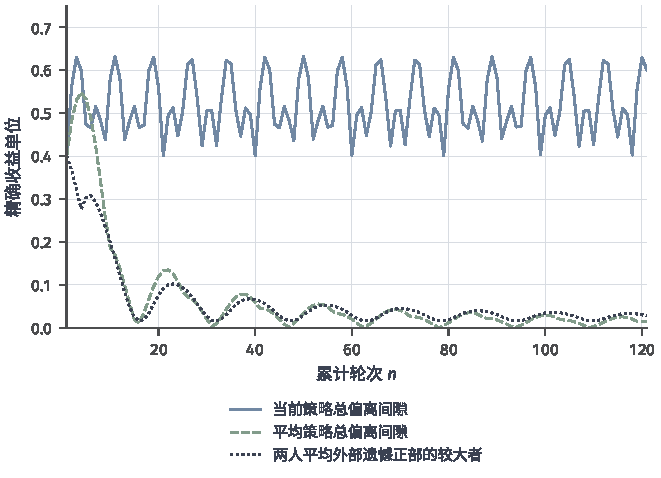
\includegraphics[width=112.000mm]{figures/10-reinforcement-learning/03-task-expansion-and-trustworthiness/matplotlib/rl-multi-agent-stability.pdf}
 \caption{同一交替梯度序列的三种检验量。当前间隙、平均策略间隙与累计平均遗憾均由精确矩阵收益计算，图源保留递推及统计公式，不代表学习基准的实验成绩。}
 \label{fig:rl-multi-agent-stability}
\end{figure}

判断保证能否沿用，需要定位每项误差作用的位置：评论家和采样误差改变收益或梯度估计，近似响应误差改变每轮与最佳响应的比较，共同学习改变下一批交互记录的分布，不完全回忆破坏信息集分解，库外策略则不在元博弈的比较类中。低外部遗憾要进一步控制平均边际策略的Nash间隙，须利用两人零和的收益抵消。一般和中通常只能得到保留相关性的联合经验分布结论，不能按相同证明推出平均独立策略达到Nash均衡。

即便阶段博弈做到了无悔，改变早先动作还会改变后面访问哪些状态。只在已访问位置比较动作，不能控制新策略将到达的位置及其后续回报。需要把后继价值向前传播，同时为未充分探索的位置保留余量。\term{V学习}（V-learning）把状态价值估计、探索与各人的局部对抗老虎机连接起来，并用训练历史构造完整的策略输出。

考虑正整数$H$和有限状态、行动空间，所有参与者在阶段$t=0,\ldots,H-1$行动前共同看到当前状态。每回合都从同一初态生成规则重新开始，转移与奖励规律可以随阶段$t$变化，但在训练回合间固定；每步奖励满足$r_{i,t}\in[0,1]$，第$H$步后终止。这里评价不折扣的整回合回报$\mathbb E\sum_{t=0}^{H-1}r_{i,t}$，与前面的无限折扣目标分开。因此，阶段$t$之后最多还有$H-t$单位回报；这一已知上界正是初始化与截断的依据。

每个参与者$i$为每个$(s,t)$保存状态价值$V_{i,t}(s)$、访问计数和一个只选择自身动作的\term{对抗老虎机}（adversarial bandit）子程序。第~\ref{sec:rl-learning-contextual}~节已说明，它用所选动作的反馈调整动作分布，以应对随历史变化的损失；此处损失会随其他人的学习而变化，不要求环境中另有恶意攻击者。价值初值为$H-t$，终端价值$V_{i,H}=0$。在$(s,t)$第$n\geq1$次访问、取得$r_i$和$s'$后，更新为
\begin{equation}
 \begin{aligned}
  \alpha_n&=\frac{H+1}{H+n},\\
  \widetilde V_{i,t}(s)&\leftarrow
      (1-\alpha_n)\widetilde V_{i,t}(s)
      +\alpha_n\bigl[r_i+V_{i,t+1}(s')+b_{i,n}\bigr],\\
  V_{i,t}(s)&\leftarrow\min\{H-t,\widetilde V_{i,t}(s)\}.
 \end{aligned}
 \label{eq:rl-multi-agent-v-learning}
\end{equation}
$\widetilde V$同样从$H-t$初始化，$b_{i,n}\geq0$是按遗憾与采样误差选取的探索余量；它使未充分采样的后果保持乐观，截断则保留已知回报上限。访问次数$n$决定更新权重，并非环境时刻$t$。局部动作子程序收到已选动作及损失$(H-r_i-V_{i,t+1}(s'))/H$，再更新自身动作分布。由于$0\leq r_i+V_{i,t+1}(s')\leq H-t\leq H$，该损失在$[0,1]$内；未选动作的损失并未全部观测，须由带相应加权遗憾保证的bandit更新处理。价值表因而不必按联合动作展开，但每个人仍需保存自己的动作概率与历史策略。

式~\eqref{eq:rl-multi-agent-v-learning}~的更新权重也规定了策略怎样混合。对已有$n$次访问的位置，第$j$次访问的历史权重为
\[
 \omega_{n,j}=\alpha_j\prod_{\ell=j+1}^{n}(1-\alpha_\ell),
 \qquad j=1,\ldots,n,\qquad\sum_{j=1}^n\omega_{n,j}=1.
\]
例如$H=2,n=2$时，$\alpha_1=1,\alpha_2=3/4$，历史权重为$(1/4,3/4)$；两份局部策略选择某动作的概率若为0.2和0.8，该次混合概率就是0.65，既不是最后一份策略的0.8，也不是均匀平均的0.5。这只演示一次局部混合。完整输出先均匀抽取训练回合索引，在每个到达的状态—时刻对，再按该索引之前的访问记录和上述权重抽取历史回合，按该回合的策略快照选择当前动作，并把抽到的索引带入下一步继续回退；未访问位置需保留初始化策略。必须保存相应计数与策略快照，不能将这一递归协议换成均匀抽取某一回合策略后整局不变。该输出一般依赖历史，不是只读取当前状态的最后一轮策略。

均衡目标决定局部遗憾和联合输出的要求。两人零和时，各人独立执行这一历史输出协议，所得乘积策略可有近似Nash保证。多人一般和时，加权外部遗憾控制对应近似CCE；若改用控制动作替换映射的加权交换遗憾子程序，则可取得近似CE。一般和的联合输出还须在执行前共享一次随机种子，同步各步抽取的历史索引，以保留所需相关性，各人的动作仍由各自策略产生。训练分散执行，并不意味着执行时可以删掉这个公共随机协议。

零和任务可按已知奖励界作正尺度变换与常数平移，采用$r_{2,t}=1-r_{1,t}$的单位区间常和计分。固定$H$时，这种等价编码保留最佳响应与均衡策略，收益误差则须按新旧尺度换算。

在上述有限表格、共同可见状态与单位区间奖励条件下，采用原论文给出的加权正则化跟随领头者（follow-the-regularized-leader, FTRL）子程序，按累计损失估计与正则项选择下一动作分布，并配合相应探索余量及完整历史输出协议。令$n_S=|S|$、$n_{A,\max}=\max_i|\mathsf A_i|$。对$\varepsilon>0$和$\delta\in(0,1)$，两人零和的$\varepsilon$-Nash与一般和的$\varepsilon$-CCE都可在
$\widetilde O(H^5n_Sn_{A,\max}/\varepsilon^2)$个训练回合后以至少$1-\delta$的概率取得；加权交换遗憾版本取得$\varepsilon$-CE的对应量级为
$\widetilde O(H^5n_Sn_{A,\max}^2/\varepsilon^2)$。这里$\varepsilon$按归一化逐步奖励的整回合收益衡量，$\widetilde O$隐藏包括失败概率和参与者数在内的对数因子，一回合至多$H$个环境步。动作规模由联合空间的乘积变为最大单人动作数，是这类结论的关键；它没有保证最后一次策略收敛，也不能直接推广到局部观测、任意神经近似或随意选取的探索余量。具体子程序与输出条件见原论文算法1、3及定理5--7\scite{rl7-jin2021vlearning}

从训练对手表现到元博弈，再到完整策略空间的最佳响应，所需验证范围逐步扩大，训练却未必自然完成这些检验。恶意通信、对抗攻击和安全约束还会改变行为要求，第\ref{chap:rl-trustworthy}章另作讨论。即便当前训练曲线稳定，也不能据此获得这些新目标的保证。

% Outline: 7.6
\section{多智能体的参与者变化适配}
\label{sec:rl-multi-agent-adaptation}

前面所有讨论都默认参与者的人数、伙伴和接口是固定的。部署时这些前提经常变化：机器人团队可能临时增加人手，合作伙伴可能换成一套从未配合过的陌生策略，竞争者也可能采用全新的行为机制。这些是性质不同的适配问题，可以沿用第\ref{chap:rl-transfer}章的训练分布、留出条件和适应预算框架，但必须把“参与者如何变化”明确写进去。跨规模、跨伙伴、跨对手分别改变的条件不同，不能因为在一种变化下协调成功，就同时声称具备了另外两种适配能力。

% Outline: 7.6.1
\subsection{参与者规模变化下的跨规模适配}
\label{sec:rl-multi-agent-scale}

先看人数变化。参与者增加时，原来为固定人数设计的策略可能连输入格式和协作约定都无法复用。例如两人网络若用固定槽位拼接“对方的位置”，就没有放入第三人的槽位；“1 先走、2 后走”的约定也没有规定第三人何时行动。

连续控制还须说明“一个参与者”控制什么。分解式多智能体集中策略梯度（factored multi-agent centralised policy gradients, FACMAC）所用多智能体MuJoCo任务按关节组控制同一系统；更换分组或观测半径会改变各人的动作集合和可见观测范围。此时即使人数相同，任务接口也可能不同，不能只比较参与者数量\scite{rl7-peng2021facmac}

对角色与动作编码相容的参与者，若编号只用于登记身份，重编号就不应改变各物理参与者的决策。把$m$人的动作前可见特征排成$\bm X\in\mathbb R^{m\times d}$，每行对应一人；邻接矩阵$\bm B\in\mathbb R^{m\times m}$记录可用的交互边。固定参数的图策略$F(\bm X,\bm B)$逐行给出各人的动作分布参数，各行使用同一动作编码。令$\bm M$为$m\times m$置换矩阵，同时重排特征行与邻接矩阵的行、列。若
\[
 F(\bm M\bm X,\bm M\bm B\bm M^\top)=\bm M F(\bm X,\bm B),
\]
就具有\term{置换等变性}（permutation equivariance）：先重编号再求策略，等于先求策略再相应重排结果。例如交换1、2两人的编号后，原1对应的策略分布应出现在新2的位置，而不是强迫两人使用相同动作。角色特征也必须随物理参与者一起重排。这是消除任意编号影响的结构要求；能够处理变长有序列表的策略不必满足它，因此变长计算与重编号对称是不同性质。

共享的邻域消息函数与不依赖邻居排列的聚合器，可以构造这种图策略：
\[
 \bm z_i=\operatorname{Agg}_{j\in\mathcal N_i}
           \phi(I_i,I_j,e_i,e_j),\qquad
 \pi_i(\cdot)=f_{\bm\theta}(I_i,e_i,\bm z_i),
\]
其中$\mathcal N_i$为$i$的邻居集合，$\phi$将一对参与者的局部特征映为消息向量，$\bm z_i$为聚合结果；此处$e_i$表示可见角色，不是任意编号，$\operatorname{Agg}$可取不依赖邻居排列的求和、均值或邻居集合上归一化的注意力。空邻域须规定合法输出，例如零向量，才能在所有图上计算策略；按身份槽位拼接一般不具有上述性质。图\ref{fig:rl-multi-agent-graph}展示同一物理图重编号后的对应。部署聚合只能使用本轮动作前实际收到的邻居消息及协议允许共享的字段，不能因图结构可写而假定邻居历史全部可见。

\begin{figure*}[htbp]
 \centering
 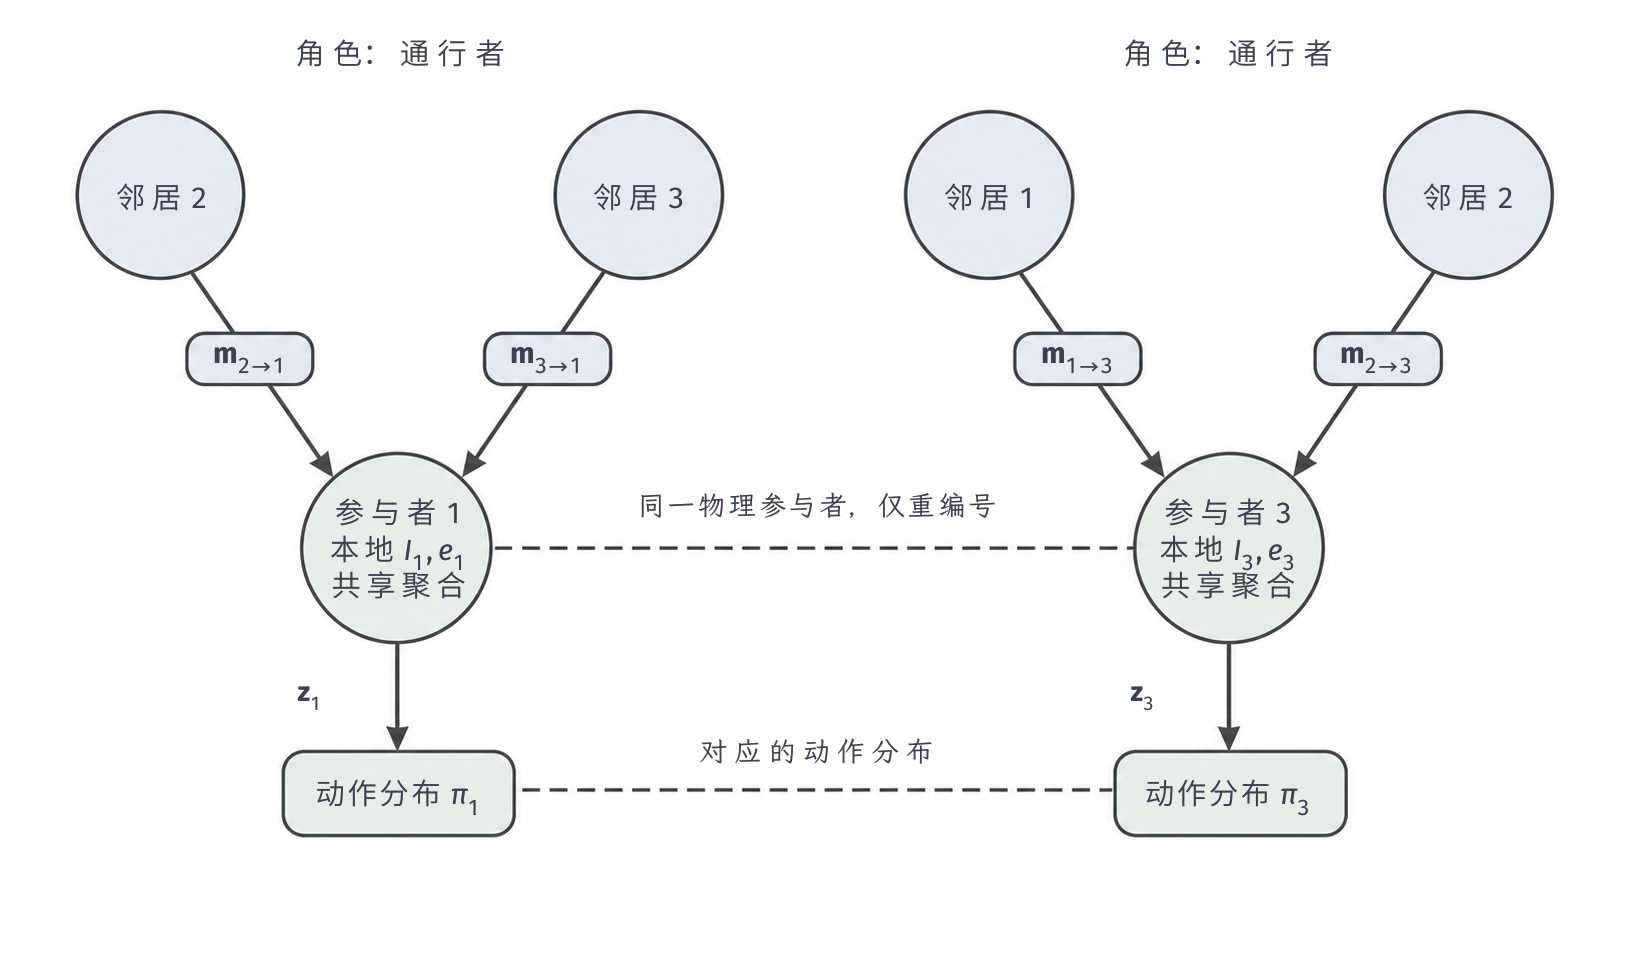
\includegraphics[width=157.400mm]{figures/10-reinforcement-learning/03-task-expansion-and-trustworthiness/generated/rl-multi-agent-graph/figure.png}
 \caption{共享邻域聚合对重编号的响应。实线把邻居消息送至本地主体，再形成动作分布；左右图仅重排同一物理节点的编号。横向虚线连接重编号前后的同一主体及相应动作分布，不是额外通信边；通行任务不变。}
 \label{fig:rl-multi-agent-graph}
\end{figure*}

当邻居很多时，逐个建模“我和每个邻居的交互”成本太高，一个自然的近似是只看群体或邻域的平均行为，把所有他人的联合影响压缩成一个“平均动作”。平均场多智能体强化学习（mean field multi-agent reinforcement learning）
\[
 \bar{\bm a}_{-i,t}
 =|\mathcal N_i|^{-1}\sum_{j\in\mathcal N_i}\bm e(a_{j,t}),
\]
其中$\bm e(a_{j,t})$为动作独热向量，求平均后得到时刻$t$实际执行后的邻域动作频率。空邻域另约定$\bar{\bm a}_{-i,t}=\bm0$，这只是无邻居标记，不是概率分布。同时行动时，参与者提交$a_{i,t}$之前不能读取尚未产生的$\bar{\bm a}_{-i,t}$；执行策略必须改用事前可得的估计$\widehat{\bar{\bm a}}_{-i,t}$。协议可以规定它由上一时刻已观察的均值、邻居策略预测，或同步求解的自洽平均场得到，但训练和评价须固定同一种构造；若通信直接公开本轮意图动作，则应把这项额外权限写入历史。已完成的联合转移可用实际$\bar{\bm a}_{-i,t}$训练评论家，而下一步TD目标中的聚合量须按同一事前规则构造$\widehat{\bar{\bm a}}_{-i,t+1}$。学习器据此将聚合行为作为$Q_i(I_i,a_i,\bar{\bm a}_{-i})$的条件。若后继目标只把事前点估计代入非线性评论家，这里采用的是点代入近似；若要计算对未来实际均值的条件期望，还需对其预测分布采样或积分。训练与评价应保留同一近似口径。原始平均场方法沿这一路线给出Q学习和行动者—评论家机制\scite{rl7-yang2018meanfield}

共享图策略可继续由联合轨迹和团队目标训练，并在训练中覆盖不同图与规模，执行时按当前邻域组装输入。令$E_G$为图边集，每轮沿各边计算消息需要$O(|E_G|)$次函数调用，传递$L$轮则乘$L$；这是固定单条消息计算结构时的调用数，不是整个网络的运行时间。网络能接受变长输入，只解决计算可定义的问题，不保证新人数$m$下回报不降。聚合方式也决定哪些局部特征差别仍可区分：求和随人数变化，均值可能丢掉邻居数量，即便置换等变也可能需要显式计数或密度特征。

平均场近似还要求个体影响较弱、聚合量足以描述交互，仅人数多并不充分。窄通道中一个关键参与者就能完全堵塞，平均前进率却未必指出谁占据瓶颈。异质角色、强配合或拓扑突变也可能使聚合量不足，所以近似有效性仍须在留出规模与交互条件下检验。

% Outline: 7.6.2
\subsection{未见合作者条件下的零样本协调与在线适配}
\label{sec:rl-multi-agent-new-partners}

换伙伴和换人数是两回事：人数不变、只换一个合作伙伴时，最容易出问题的不是技能，而是双方默认的协调约定是否兼容。

Overcooked的共享烹饪任务中也有这种区别。同一厨房下，与共同训练的伙伴完成分工，不代表能与新伙伴保持同样配合；评价须给出伙伴来源，并规定双方是否允许适应\scite{rl7-carroll2019}

先按第\ref{sec:rl-transfer-budget}节区分零样本与适应预算。本章对\term{零样本协调}（zero-shot coordination）采用同样的严格预算口径：不使用新伙伴反馈作伙伴特定的参数更新、记忆适应、类型辨识或模型选择，但可读取已给角色、约定及正常控制所需的观测。在给定任务和伙伴模型下估计当前位置，仍属普通状态估计；利用伙伴动作或回报改变对其行为类型的判断，则已发生适应。即使这一判断只在首回合内更新、网络参数始终固定，也不能按本章口径称为零样本。

文献中的zero-shot coordination有时主要强调测试伙伴未与当前策略共同训练；是否允许首回合内利用伙伴反馈，还须读取具体协议。将这些结果按本章分类时，应按实际反馈、记忆重置与参数更新权限归类。

\term{临时团队协作}（ad hoc teamwork）研究未预先共同训练或充分协调的新队伍，协议可以允许交互辨识和伙伴适配。为确定其可行策略，实验须说明是否共享左右约定、能否通信、角色是否可见、允许试探几步，以及试探失败的代价。任务名称并不自动提供这些权限。

机制选择须与可读任务约定、伙伴类型线索和交互历史对应。扩大训练伙伴群体要有多类伙伴可供交互，处理对称性要知道哪些变换保持任务不变，伙伴条件策略要有部署时可见的类型线索，在线信念更新则要有能区分类型的历史。Other-Play利用所给任务对称性，减少策略对某次自我对弈任意约定的依赖；作用范围仍由该对称性与协调条件限定，不能保证兼容任意未知伙伴\scite{rl7-hu2020otherplay}

一种在线协议先冻结基础策略与类型模型，在前$B$步用获准动作或消息收集证据，再按第\ref{sec:rl-multi-agent-opponent-model}节更新信念，以伙伴条件价值选动作。若还允许梯度适配，须另计更新次数和目标伙伴交互训练记录的来源。报告应区分零样本、仅记忆或信念适应、参数适应，并说明回合内及跨回合的记忆保留。适应后评价可继续估计物理状态，但只要反馈仍修正伙伴类型，适应过程就没有结束；若两者无法分离，也应据实计入协议。交互数量增加不保证类型可辨识，证据不足时仍可能无法区分伙伴。

最后，分工还受观测、历史和角色信号的对称性限制。双方若使用同一确定性策略、取得同一历史，又没有身份、方位或指定不同角色的公共信号，所选动作就相同，无法保证恰好一人前进。独立随机化提供打破对称的机会，却不能保证本轮形成指定分工。合法公共角色信号能改变可行策略集合，因此使用它时须在评价协议中明示。

% Outline: 7.6.3
\subsection{未见竞争者条件下的策略适应}
\label{sec:rl-multi-agent-new-opponents}

面对新竞争者，还要在“针对已知弱点尽量榨取收益”和“对手一变也不至于被反制”之间权衡。

对手条件策略可以先在训练群体中学习行为表示，部署时据可见动作、回合结果或消息更新类型信念，再选择响应。优化目标可以是给定对手分布下的收益，也可以另加已知策略类中的最坏情形限制；比较适应速度前必须先说清使用哪种目标。表\ref{tab:rl-multi-agent-opponent-adaptation}列出相应比较对象，并区分固定对手与随自身行为响应的对手。

\begin{table}[htbp]
 \centering
 \begin{tabularx}{\linewidth}{@{}l >{\raggedright\arraybackslash}X >{\raggedright\arraybackslash}X@{}}
 \toprule
 问题 & 对手、历史及允许更新 & 比较对象\\
 \midrule
 固定对手最佳响应 & 目标固定；可交互观测；按给定预算更新 & 同一对手下可行最佳响应收益\\
 群体内适应 & 见过类型的新抽样；允许历史辨识或少量更新 & 同预算的群体条件基线及零样本策略\\
 跨对手泛化 & 未见行为类型；历史与反馈权限明确 & 留出类型的平均、尾部及最坏已测收益\\
 反应型对手适应 & 对方可随自身行为改变；响应历史需记录 & 声明响应协议下的序贯收益，非固定对手值\\
 \bottomrule
 \end{tabularx}
 \caption{对手适应的目标与可用证据。需同时给出类型留出、记录采集与访问权限和比较对象；同一策略只更换随机种子并未构成类型留出。}
 \label{tab:rl-multi-agent-opponent-adaptation}
\end{table}

例如，规定20场探测再评价100场时，还须确定探测是否计分、记忆是否重置、梯度步上限，以及对手在全部120场中是否保持不变；这些数字仅定义教学预算。响应训练使用的对局不能同时充当独立测试。对手若先以温和行为诱导信念、随后切换，或在探测中继续学习，固定类型模型就可能不适用。此时须按第\ref{sec:rl-multi-agent-response-model}节重新规定响应机制，不能保留固定类型识别的保证。

% Outline: 7.6.4
\subsection{参与者变化适配的泛化与扩展边界}
\label{sec:rl-multi-agent-generalization}

无论测试跨规模、跨伙伴还是跨对手的适配，都应先声明究竟变化了哪个因素，并据此划分训练、验证与测试的参与者及交互记录；把多种变化混在同一批“新环境”测试里，成功或失败都无法归因。

\begin{table}[htbp]
 \centering
 \begin{tabularx}{\linewidth}{@{}l >{\raggedright\arraybackslash}X >{\raggedright\arraybackslash}X@{}}
 \toprule
 变化因素 & 可声明的留出方式 & 必须控制或记录\\
 \midrule
 数量与密度 & 训练2至4人，测试6人等独立设定 & 通道容量、拥挤度、邻域大小，不能只改$m$\\
 身份与组合 & 已见类型的新排列、新搭配 & 角色是否同构；是否共享编号约定\\
 合作者或对手类型 & 留出训练流程、策略家族或行为机制 & 零样本／适应预算；伙伴是否继续学习\\
 收益关系 & 固定关系内的新参数，或另测关系改变 & 团队转竞争已改变目标，不能仅称身份泛化\\
 通信与拓扑 & 留出图、延迟、带宽或接收范围 & 部署消息是否可得；公共信号是否保留\\
 \bottomrule
 \end{tabularx}
 \caption{参与者变化的留出方式与控制条件。支持内的新搭配和未见行为类型不是同一种测试，其覆盖与辨识要求不同。}
 \label{tab:rl-multi-agent-splits}
\end{table}

同一批伙伴更换环境种子，只检验给定伙伴下的运行随机性；同一策略更换编号，至多检验身份依赖。若同时改变人数、角色、奖励和通信，失败不能单独归因于规模，成功也难以辨认是哪项适配有效。因此应先作单因素留出，再评价明确的组合变化，结论范围始终受实际留出因素限定。

% Outline: 7.7
\section{多智能体的行为评价和验证}
\label{sec:rl-multi-agent-evaluation}

最后是评价。多智能体系统的“好”有多个互不替代的侧面，必须分别检验：策略取得了多高的收益？是否满足选定的行为标准（有没有单方面偏离的动机）？能否和声明范围内的新伙伴、新对手正常交互？又花费了多少资源？基准回报说明任务表现，偏离搜索检查稳定性，交叉配对检查约定是否兼容，资源统计说明代价。把这些量压成一个无条件的单一排名，会丢掉各自的验证范围。

% Outline: 7.7.1
\subsection{共同评价目标下的效用、福利与公平评价}
\label{sec:rl-multi-agent-welfare}

评价收益时应先回到各方原本的目标，不能用一个总分掩盖分配差异。

例如，教学结果$(10,0)$与$(5,5)$总收益都为10，最小收益分别为0和5，个体收益的总体方差分别为25和0。若第一种结果总由同一人承担成本，只报团队总分便看不到差异；若角色按公平规则轮换，还需区分单回合和长期分配。实际评价应至少报告均值、分布与失败率，并定义失败究竟是碰撞、超时还是某人的任务未完成。

指标还须对应具体任务接口，表\ref{tab:rl-multi-agent-benchmarks}为此区分环境库中的任务。例如，星际争霸多智能体挑战（StarCraft multi-agent challenge, SMAC）考察局部观测下的团队微操，即多个受控单位分别选择移动、攻击等战斗动作；地图和敌人脚本共同决定难度与胜率含义，不能只写环境库名称来确定评价条件\scite{rl7-samvelyan2019}。表中的MPE指多智能体粒子环境（multi-agent particle environment），其收益、观测与通信同样由具体任务配置决定。

\begin{table*}[t]
 \centering
 \begin{tabularx}{\linewidth}{@{}l >{\raggedright\arraybackslash}X >{\raggedright\arraybackslash}X >{\raggedright\arraybackslash}X >{\raggedright\arraybackslash}X@{}}
 \toprule
 具体接口 & 合作或竞争结构 & 可用观测 & 通信条件 & 主要指标\\
 \midrule
 SMAC，3m & 三个受控单位合作，对抗脚本敌人 & 各自视野内的单位特征；训练可给全局状态 & 原任务无额外学习消息，新增须声明 & 地图胜率、回报、超时率\\
 MPE，simple\_spread & 多个体覆盖地标；局部碰撞项与共享项比例需指定 & 自身及其他实体的配置相关特征 & 此任务的静默体无消息；不能外推至其他MPE任务 & 覆盖距离、碰撞及所定奖励\\
 Overcooked，cramped\_room & 两人完成共享烹饪与交付任务 & 厨房布局、物品及参与者状态的指定编码 & 原动作接口无自由语言频道 & 交付数、团队回报、分工及等待\\
 PettingZoo，rps & 两人石头剪刀布，零和 & 本轮选择在双方提交前相互隐藏 & 无显式消息；AEC调用次序不等于看见先行动作 & 各自收益及偏离间隙\\
 多智能体MuJoCo，分组HalfCheetah & 不同关节组共同控制同一系统 & 分组关节特征及指定观测半径 & 消息或额外关节状态需另列 & 回报、预先定义的失稳事件率、推理时延\\
 \bottomrule
 \end{tabularx}
 \caption{具体任务接口的收益、可见观测与评价指标。复现还须固定软件版本、地图、观测包装器、奖励配置及回合上限，不能只指定环境库。}
 \label{tab:rl-multi-agent-benchmarks}
\end{table*}

多智能体粒子环境中的收益和通信配置因任务而异，一个任务采用静默动作不能说明整个环境族都无通信。Overcooked还应将共同训练伙伴与新伙伴的结果分开，才能对应第\ref{sec:rl-multi-agent-new-partners}节所区分的协调能力。

PettingZoo石头剪刀布的检验重点包括屏蔽对方本轮尚未提交的动作。调用程序可以先保存一人的动作，另一人的策略却不能据此选择本轮动作；这正是第\ref{sec:rl-multi-agent-information}节所要求的调用顺序与可见时序分离。

连续控制则须按第\ref{sec:rl-multi-agent-scale}节记录关节分组和每组可见的关节状态，仅写“MuJoCo”不能确定控制接口。改变人数或观测半径也会改变协调条件，相应结果不能当作同一问题直接比较。

不同接口的动作粒度、回合长度和奖励尺度不同，原始分数不能直接求和。评价时提供给行动者的观测、消息及送达时序须与部署一致，不应额外提供全局状态或免费通信。若训练使用奖励塑形，宜同时给出原任务指标与实际优化回报，以区分塑形目标提高和任务确实完成。

% Outline: 7.7.2
\subsection{行为标准下的偏离收益、遗憾与可利用性验证}
\label{sec:rl-multi-agent-deviations}

平均回报高，并不代表这个局面是稳定的——也许某个参与者稍作改变就能获得更大好处。因此还要专门检查单方偏离标准：固定其他人的完整策略，搜索$i$在相同的行动前观测、历史与消息权限下能找到的最好替代策略，并比较两者回报。
\[
 \delta_i(\bm\pi)=
 \sup_{\pi_i'\in\Pi_i}J_i(\pi_i',\bm\pi_{-i})-J_i(\bm\pi).
\]
比较类$\Pi_i$必须保留原观测、消息与行动权限，并含当前$\pi_i$；不作改变就是其中一种选择，故$\delta_i\geq0$。两人零和时，本章将双方偏离收益相加，记总间隙$g=\delta_1+\delta_2$。部分软件以$g/2$称为可利用性，报告中要标明采用的约定。

匹配硬币中取$p=0.7,q=0.4$，当前$u_1=-0.08$。固定$q$，1改为第二动作得0.2，偏离收益$\delta_1=0.28$；固定$p$，2改为第二动作使1得$-0.4$，自身从0.08升到0.4，故$\delta_2=0.32$。总间隙为0.6，按半间隙约定为0.3。只对均匀对手测得零回报，无法发现这种能被针对性响应利用的偏好。

第\ref{sec:rl-multi-agent-mutual-learning}节介绍了产生低遗憾的机制。下面从遗憾定义推导可验证的结论，并保留其中的联合分布与零和条件。

固定正整数$n$与$\varepsilon\geq0$，将各人非空有限动作集上的固定有限阶段博弈重复$n$轮，实际联合动作为$\bm a^{(k)}$，按联合动作频率定义经验分布
$\hat q_n(\bm a)=n^{-1}\sum_{k=1}^n\mathbf1\{\bm a^{(k)}=\bm a\}$。
若每个人对每个固定替代动作的累计外部遗憾都不超过$n\varepsilon$，则$\hat q_n$满足$\varepsilon$粗相关均衡约束。若进一步对每对动作$a_i,b_i$，仅在实际选$a_i$的轮次改用$b_i$的内部遗憾满足
\[
 \sum_{k=1}^n\mathbf1\{a_i^{(k)}=a_i\}
 [u_i(b_i,\bm a_{-i}^{(k)})-u_i(\bm a^{(k)})]
 \leq n\varepsilon,
\]
则$\hat q_n$满足每对动作的未条件化$\varepsilon$相关均衡偏离约束。
这个结论按联合动作频率合并遗憾和：外部遗憾对应事前固定偏离，内部遗憾只保留实际建议为$a_i$的轮次，因此对应未条件化的建议替换。两者都保留联合频率，不要求各人的动作独立；它们用于检验重复交互的经验行为标准，不能单凭它们认证最后一轮策略已经收敛。

若改为评价收到$a_i$后的条件收益，需要两边同时除以建议概率$\hat q_{n,i}(a_i)$，条件误差界成为$\varepsilon/\hat q_{n,i}(a_i)$，对罕见建议可能很大。零概率建议不需定义条件期望。若允许同时替换多个建议，逐对约束的误差相加还会累积，不能直接把每对动作的$\varepsilon$解释为任意交换映射的同一界。

保留联合频率是结论成立的关键。协调约定$(L,L)$和$(R,R)$各占一半时，经验分布从不失配，但各人边缘都是均匀分布；取边缘乘积就出现$1/2$的失配概率。一般和的低遗憾控制前一种相关分布，通常不控制后一种独立边际平均策略的Nash偏离。

固定正整数$n,p,q$与$\varepsilon_1,\varepsilon_2\geq0$，考虑有限两人零和收益矩阵$\bm A\in\mathbb R^{p\times q}$。第$k$轮采用混合策略$\bm x^{(k)}\in\Delta_p,\bm y^{(k)}\in\Delta_q$，候选集合为全部行、列动作概率分布。若按期望收益计算的双方累计外部遗憾分别不超过$n\varepsilon_1,n\varepsilon_2$，则各自平均策略
$\bar{\bm x}=n^{-1}\sum_{k=1}^n\bm x^{(k)}$、$\bar{\bm y}=n^{-1}\sum_{k=1}^n\bm y^{(k)}$满足
\[
 \max_{\bm x\in\Delta_p}\bm x^\top\bm A\bar{\bm y}
 -\min_{\bm y\in\Delta_q}\bar{\bm x}^\top\bm A\bm y
 \leq\varepsilon_1+\varepsilon_2.
\]
左侧是这对平均策略的总单方偏离间隙，用于把双方无悔证据转成平均策略的均衡误差。收益对各方混合策略的线性性允许按轮次平均，而两人零和使双方遗憾中的当前收益和相消；一般和时不能沿用这个抵消。这个界约束适当平均策略，不要求最后一轮策略收敛。

若统计的是实际纯动作及其实际遗憾，可把纯动作当作单纯形顶点，沿用此论证。若只有期望遗憾界，要作高概率经验声明还需相应集中界。一般和中两人收益不互为负数，当前收益项不能如此消去，因而同一推导不能给出Nash结论。

用于有限扩展式博弈时，可将完整确定性应对计划视为纯策略，并在完全回忆下用式\eqref{eq:rl-multi-agent-average-behavior}恢复平均实现计划。用于随机博弈时，还须明确比较完整策略偏离、状态条件偏离还是给定轨迹的局部替换。完整策略改变会改变后续状态访问，原轨迹上逐步动作遗憾的和不能直接控制这些新状态中的收益。表\ref{tab:rl-multi-agent-guarantees}据此区分验证对象和访问要求。

\begin{table}[htbp]
 \centering
 \begin{tabularx}{\linewidth}{@{}l >{\raggedright\arraybackslash}X >{\raggedright\arraybackslash}X@{}}
 \toprule
 指标 & 对象与计算权限 & 可支持的结论\\
 \midrule
 固定对手回报 & 对某对手的重复对局 & 该对手分布下的收益，非均衡认证\\
 阶段外部／内部遗憾 & 固定阶段收益；需替代动作收益或受控估计 & 联合经验的CCE／相应CE约束\\
 平均策略间隙 & 两人零和；完整比较类的双方遗憾或响应 & 该平均策略及策略类下的偏离界\\
 当前策略可利用性 & 固定当前对方，分别搜索并评价最佳响应 & 精确响应给间隙；近似响应通常只揭示下界\\
 \bottomrule
 \end{tabularx}
 \caption{偏离相关评价量所需的对象与权限。对平均策略取得保证，不等于已认证当前策略；近似搜索和精确响应也提供不同强度的证据。}
 \label{tab:rl-multi-agent-guarantees}
\end{table}

实际搜索若只找到$\tilde\pi_i$，其真实偏离收益不超过$\delta_i$，故只能揭示可利用性的下界。没有找到强响应，不能证明强响应不存在。若另证搜索误差$\eta_i$，即最佳响应值至多高出已找到值$\eta_i$，才可给出相应上界；有限对局估值还须加统计不确定性。宜分别保留用于拟合响应策略的训练样本、用于筛选响应的验证样本，以及选择结束后用于最终估值的测试样本，既避免把搜索中的偶然高分当作真实漏洞，也避免以搜索失败认证不可利用。

% Outline: 7.7.3
\subsection{基于交叉对局与留出参与者的泛化验证}
\label{sec:rl-multi-agent-cross-play}

要评价策略对陌生伙伴的泛化能力，必须先说明测试参与者是从哪里来的：训练伙伴、独立训练的新策略、还是从未见过的整个策略家族。不同来源检验的能力完全不同，不能用更多对局数来替代“留出”这一设计。

图\ref{fig:rl-multi-agent-cross-play}用两约定教学任务比较前两种协议。同一约定得团队分10，不同得0；独立训练来源A、B都固定采用$L$，来源C固定采用$R$。矩阵行列表示训练来源，而非同一网络不同回合的随机数。三格主对角均得10，A、B与C交叉配对却得0，说明只看同来源结果会遗漏约定不兼容。

\begin{figure}[htbp]
 \centering
 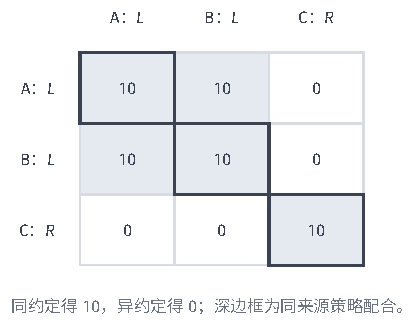
\includegraphics[width=69.977mm]{figures/10-reinforcement-learning/03-task-expansion-and-trustworthiness/tikz/rl-multi-agent-cross-play.pdf}
 \caption{两约定任务的交叉配合矩阵。各格给团队分，深边框标同来源对角；A、B使用$L$，C使用$R$，不兼容配对得0。数值由教学规则精确计算，并非实测成绩。}
 \label{fig:rl-multi-agent-cross-play}
\end{figure}

测试前应冻结训练群体、检查点选择和各伙伴的对局预算。可先对每个留出伙伴测零样本结果，再在预设$B\in\{0,5,20\}$等教学预算网格上测适应后表现；横轴记录实际交互，另列梯度步及记忆重置规则。若反复利用测试对手结果选检查点，它已被用于开发，需要重新留出，而非继续称为未见。

图中九格均匀平均为$50/9$，最差格为0，只平均三格对角却得到10。伙伴分布改变时，加权平均也改变，因此应同时报告矩阵、权重、平均和最坏已测表现。有限对局并未穷尽所有对手，最坏已测值仍不同于完整策略空间的最坏值，群体平均也不能提供不可利用性上界。

% Outline: 7.7.4
\subsection{固定样本、通信与计算预算下的效率评价}
\label{sec:rl-multi-agent-efficiency}

多智能体系统的资源消耗比单人复杂得多（一个联合环境步里其实包含$m$个参与者的动作），因此评价效率前必须统一计数口径，否则“更快”可能只是少算了某些通信或对手对局。

表\ref{tab:rl-multi-agent-resources}在每人$A$个离散动作、图边集$E_G$、消息维度$d_c$和消息传递轮数$L$的条件下，比较结构性操作成本。采样统一计联合步数$N$，达到某回报所需的$N$仍须实测。表中的计算阶数只说明列出的操作如何增长，不构成样本需求的推导。

\begin{table*}[htbp]
 \centering
 \begin{tabularx}{\linewidth}{@{}l >{\raggedright\arraybackslash}X >{\raggedright\arraybackslash}X >{\raggedright\arraybackslash}X >{\raggedright\arraybackslash}X@{}}
 \toprule
 结构 & 人数与动作计算 & 采样及训练权限 & 训练通信／存储 & 部署推理与通信\\
 \midrule
 联合价值枚举 & $m$人，$A^m$组合 & $N$联合步；集中输入 & 联合转移、动作与价值表或网络 & 若集中选动作，须具备实时集中权限\\
 VDN／QMIX & 局部比较$mA$次 & $N$联合步；QMIX混合器用状态 & 联合TD目标及训练反传 & $m$次局部网络；无必需执行消息\\
 集中评论家、局部行动者 & 每人一次动作输出 & $N$联合步；声明评论家状态／动作输入 & 回放或近期轨迹及集中特征 & 局部推理；共享参数不等于共享观测\\
 图消息策略 & $m$节点、$|E_G|$条边 & $N$联合步；合法训练图 & 消息及历史按实现记录 & $L|E_G|d_c$量级消息元素，$L$轮同步\\
 PSRO群体 & 双方各$K$个库策略 & 响应样本加收益表对局；权限继承响应器 & $K^2$表项及多个检查点 & 回合抽索引再执行；未必同时运行全部网络\\
 \bottomrule
 \end{tabularx}
 \caption{训练与部署的结构性资源需求。所列复杂度只针对对应操作，不等于总运行时间，也不证明达到某一回报的样本复杂度。}
 \label{tab:rl-multi-agent-resources}
\end{table*}

消息拓扑对成本的影响可由图\ref{fig:rl-multi-agent-scaling}的串行模型说明。设每条有向边处理一条消息耗时0.01毫秒，全部节点动作计算耗时$0.05m$毫秒。全连接具有$m(m-1)$条边；局部图在此按每人恰向$\min(4,m-1)$个出邻居发消息计算，共有$m\min(4,m-1)$条边，这是“最多4个”的满额情形。按节点和边逐项相加，得到
\[
 \begin{aligned}
 T_{\text{全连}}(m)&=0.05m+0.01m(m-1),\\
 T_{\text{局部}}(m)&=0.05m+0.01m\min(4,m-1).
 \end{aligned}
\]
代入$m=20$，两种解析时延分别为4.8和1.8毫秒。它们只成立于所给串行模型，并非硬件测试；真实设备的并行、拥塞及同步开销都可能改变结果。

\begin{figure}[htbp]
 \centering
 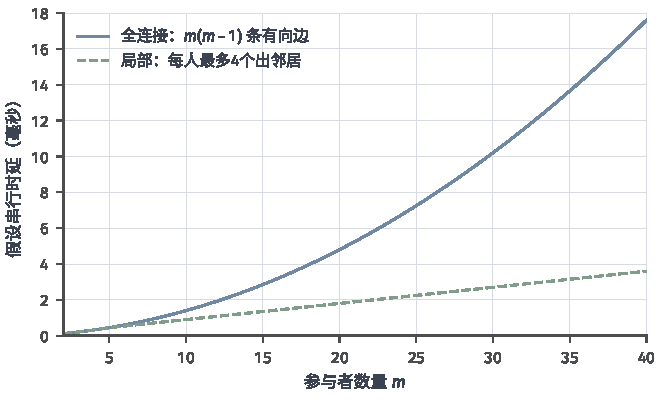
\includegraphics[width=112.000mm]{figures/10-reinforcement-learning/03-task-expansion-and-trustworthiness/matplotlib/rl-multi-agent-scaling.pdf}
 \caption{串行消息模型中的跨规模成本。全连接与最多4邻居的局部交互采用相同节点和边成本；稀疏图降低消息量，但可能同时删去任务需要的远端参与者状态或消息。}
 \label{fig:rl-multi-agent-scaling}
\end{figure}

资源比较应保留这些取舍：复用同一结构的参数可减少模型存储，却仍须为不同历史计算动作；集中状态与联合历史可帮助估计，却增加训练传输；通信可改善协调，却增加收发与同步开销，是否增加总时延还取决于并行实现。跨规模测试还须控制拥挤度、瓶颈容量和观测、历史与消息读取权限，否则成本增长与任务难度变化混在一起，难以解释曲线。

% Outline: 7.7.5
\subsection{行为评价与复现所需的协议信息}
\label{sec:rl-multi-agent-protocol}

多智能体结果尤其难复现，因为即使恢复了网络参数和随机种子，只要训练时的对手配对、各人行动前可读取的观测、历史与消息等交互条件没还原，结果就可能完全不同。因此复现不仅要恢复参数和随机种子，还须恢复参与者配对与交互权限。

\begin{table*}[htbp]
 \centering
 \small
 \begin{tabularx}{\linewidth}{@{}l >{\raggedright\arraybackslash}X >{\raggedright\arraybackslash}X@{}}
 \toprule
 协议项 & 必须记录的内容 & 主要影响环节\\
 \midrule
 参数共享与身份 & 共享哪些模块；编号、角色编码及重排规则 & 参数梯度汇总与执行约定\\
 集中状态与屏蔽 & 评论家输入；合法动作掩码由谁提供 & 训练权限及执行动作分布\\
 死亡、退出与终止 & 占位观测、动作、损失屏蔽；全局或个体终止 & 价值目标、占用统计和人数\\
 回放与版本 & 来源检查点、窗口、概率字段、校正与采样权重 & 联合经验的目标匹配\\
 对手与伙伴抽样 & 库版本、保留及淘汰、抽样概率、是否在线学习 & 训练和评价的参与者分布\\
 通信 & 发送／接收权限、载荷、时序、延迟、带宽 & 部署可行性与成本\\
 回报与评价 & 奖励尺度、塑形、回合上限、偏离类及间隙约定 & 行为标准和比较口径\\
 \bottomrule
 \end{tabularx}
 \caption{复现多智能体结果所需的最小协议。各项可能改变策略、环境或验证对象，因此超参数表之外还需保存这些交互条件。}
 \label{tab:rl-multi-agent-protocol}
\end{table*}

还应保存伙伴与对手的生成流程、策略库和检查点标识、用于检查点选择的验证参与者，以及各组合的评估场数。训练初始化、环境随机性和伙伴抽样宜采用可追踪的独立随机源。若5次独立训练各评价1000局，独立训练运行仍只有5个，不能把5000场对局当作5000次独立训练。同一检查点或同一适应链上的对局可能相关，区间估计应保留训练运行与伙伴层级。

第三方对手、外部游戏版本或消息服务若无法恢复，应列明限制。所存材料可以支持在这些伙伴与接口下重现结果，未必支持对所有未知参与者成立。只有声明、协议和证据对应同一对象，评价范围才清楚。

% Outline: 7.8
\section{本章小结}
\label{sec:rl-multi-agent-summary}

同一个通道动作会随对方行为产生不同后果，因而多智能体求解要先明确收益、观测与消息权限及参与者变化。收益关系决定采用团队最优、极小极大还是单方偏离标准，社会分配目标须另行规定；观测与消息读取权限限定策略可依赖的历史字段，集中训练不能扩大部署可见范围；其他人继续学习时，边缘化后的行为后果也可能不再平稳。

经验采集须记录联合动作、消息与参与者来源，并检查目标的联合支持；边缘动作都出现过，仍可能无法识别所需的配合效果。在此基础上，联合价值、个体替代、局部组合、伙伴类型和响应模型保留不同依赖，可共同提供更新所需的估计。价值或梯度计算还须与相互适应和群体组织配合。局部贪心一致不等于整表可表示，单次改进不等于共同动态稳定，库内近似响应也不能认证完整博弈不可利用。

验证时，外部与内部遗憾分别约束粗相关和相关经验分布；利用零和抵消才能进一步控制适当平均策略的鞍点间隙，当前策略却未必收敛。训练对手收益、留出伙伴协调、跨规模表现与资源成本也须分别报告。使用伙伴反馈更新记忆或类型已属适应，即使参数不变，也不能记为零样本。明确行为标准、参与者范围、可读观测与消息和交互预算之后，结果才有可解释的边界。第\ref{chap:rl-trustworthy}章将转向风险、扰动和安全约束这一类行为要求；性能证据并不自动成为安全保证，多方任务仍需保留本章的联合行为、局部观测与消息时序条件。

% Outline: 8
\chapter{可信强化学习}
\label{chap:rl-trustworthy}

前几章评价一个策略时，默认问题几乎只有一个：它的期望回报有多高。这个标准在多数回合表现正常时足够好用，却回答不了一类更尖锐的问题——“出状况的那几次怎么办”。考虑一台导航机器人：它在大多数回合很快到达终点，只在少数回合严重延误。平均到达时间即使很短，也把顺利回合和糟糕回合混在了一起，无法说明这些延误是否可以承受。更麻烦的是，训练时假设的环境与部署时未必相同：地面变湿时，原来学到的制动规律可能整体失效；而在机器人上启用一个会在危急时刻接管的紧急保护器后，“没有碰撞”又可能只是保护器替换了危险动作的结果，并不能说明原策略本身可靠。于是部署判断需要回答两个层次不同的问题：第一，我们究竟希望机器人满足什么行为要求——是平均表现好，还是最差的回合也不能太糟，是湿滑地面也要能用，还是任何时候都不许碰撞；第二，手头的证据——无论是有限的试验记录还是基于模型的证明——是否足以支持这些要求。前者是在规定“什么算合格”，后者是在核查“凭什么相信它合格”。

本章沿用第~\ref{chap:rl-overview}~章的策略与轨迹，以及第~\ref{chap:rl-planning}、\ref{chap:rl-learning}~章的规划和学习工具。回答第一个问题时，三种要求分别从三个不同的环节收紧决策：风险敏感决策改变的是随机后果的评价方式，例如不再只看平均损失，而比较最差那部分回合的损失；鲁棒决策改变的是环境范围，要求同一策略在允许的环境变化下都维持表现；安全约束改变的是可行策略集合，把不满足成本预算或边界要求的策略直接排除。三者改动的对象不同，可以组合使用，但并无必须依次采用的演进顺序。求出候选策略后，第二个问题——证据——才登场：此时评价一个已经冻结的策略、评价一条固定学习规则重复训练出的多个策略、以及评价一个带保护器的完整执行系统，是三种随机性来源不同、结论也不同的取证任务，必须分开处理。

图~\ref{fig:rl-trustworthy-map}~将三类要求放在相同的任务设定下。各分支先给出要维护的性质和求解方法，再由验证过程检查候选方案；方案比较中的保证只在相应运行条件和证据范围内成立。

\begin{figure*}[t]
  \centering
  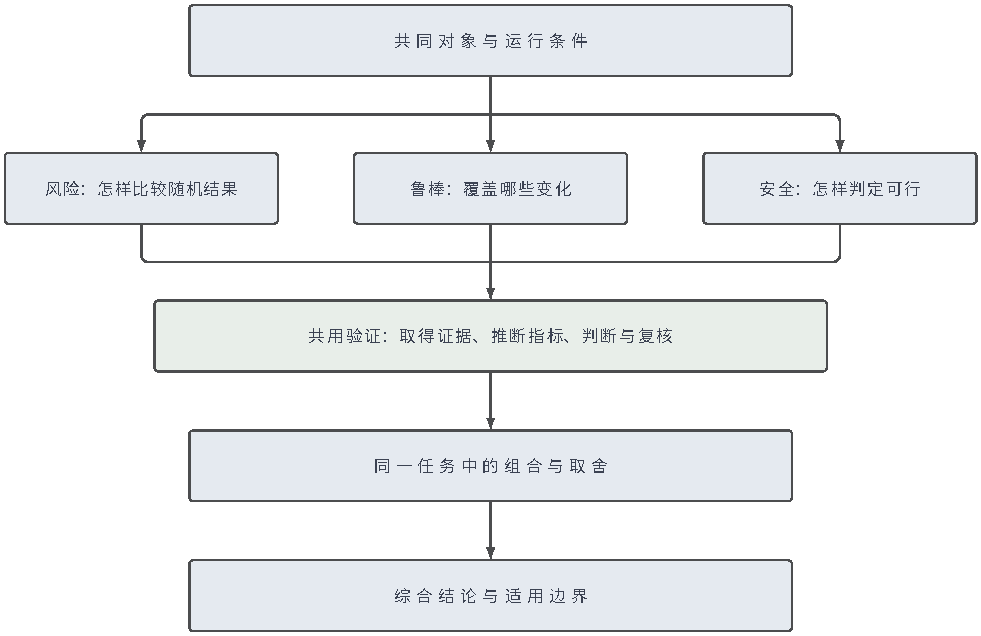
\includegraphics[width=166.169mm]{figures/10-reinforcement-learning/03-task-expansion-and-trustworthiness/tikz/rl-trustworthy-map.pdf}
  \caption{可信强化学习的章内关系。共同设定固定决策对象和运行条件，三个分支提出行为要求与候选策略，验证过程据此判断组合方案。箭头表示模型、策略、验证记录与结论之间的依赖，不表示风险、鲁棒与安全必须依次执行；综合结论仍保留各分支的适用条件。}
  \label{fig:rl-trustworthy-map}
\end{figure*}

% Outline: 8.1
\section{行为要求与保证对象}
\label{sec:rl-trustworthy-requirements}

要把上面三个要求讲清楚，先得学会做“只改一项条件”的受控比较——如果好几个因素同时变化，观察到的成功率改变就无法归因。仍考察从起点驶向终点的移动机器人。在相同的几何路线、初始位置与动力学下，比较不同速度控制策略诱导的到达时间分布，可以检查偶发严重延误；固定策略与目标，改变地面摩擦，可以检查制动距离。若环境不变，只把一块原本可以穿越的地带声明为危险区，改变的则是行为是否被允许的判定标准。最后，启用会替换危险动作的保护层，改变了实际执行机制。四种比较各自只改变一项条件，因而能够分别识别结果分布、环境变化、行为可行性和保护器的影响；一个总成功率无法区分这些影响。

离散导航示意沿用宽4、高3的网格、起点$(1,1)$、终点$(4,3)$和障碍$(2,2)$。数值例子会分别声明采用基准滑移模型，还是把整段路线汇总为一次选择的教学模型；路线模型用于手算，不是随机网格的精确解。连续控制仍写作$\bm{x}_{t+1}=\bm{A}\bm{x}_t+\bm{B}\bm{u}_t+\bm{w}_t$，状态可以包含位置和速度；允许扰动$\bm{w}_t$的范围来自另行给定的运行条件，不能从动力学方程本身读出。

在给出具体要求之前，先要统一描述“一次运行会产生什么、我们又能测量什么”，因为后面三类准则比较的正是这些不同的量。同一回合既可能效率高，也可能靠近过危险区，还可能发生碰撞；只用一个标量回报无法同时表达这些后果。下面先固定评价对象，再谈怎样用它们提要求。

\begin{definition}[回报、损失、成本与失败事件]
  \label{def:rl-trustworthy-objects}
  固定动态环境$\mathcal E$、观测与反馈机制和策略$\pi$，得到理论轨迹律$P_{\mathcal E}^\pi$；实际可取得的评价记录服从$P_{\mathrm{rec}}^\pi$。若损失含未记录状态，还须说明能否由这些记录识别损失的分布。记相应的轨迹样本空间为$\Omega_{\mathrm{traj}}$，其事件$\sigma$代数为$\mathcal F_{\mathrm{traj}}$（即我们能对其讨论“发生概率”的那些轨迹集合，例如“所有发生过碰撞的轨迹”构成的集合）。无限时域取$0\leq\gamma<1$，并要求下面的奖励和成本级数绝对可积；有界逐步奖励与成本足以满足这一条件。
  对轨迹$\tau=(s_0,a_0,r_0,s_1,\ldots)$，回报为
  $G(\tau)=\sum_{t\geq0}\gamma^t r_t$，目标$J(\pi)=\mathbb E_\pi G$不作归一化。
  损失$L(\tau)$表示需要抑制的后果，数值越大越差；它可以是累计延误，也可以是$-G$，但必须明确选择。
  安全成本$c_{i,t}\geq0$记录第$i$类危险暴露或损害，其累计量为
  $C_i(\tau)=\sum_{t\geq0}\gamma^t c_{i,t}$。
  失败事件$F_H\in\mathcal F_{\mathrm{traj}}$是轨迹空间中的可测事件，因而$F_H\subseteq\Omega_{\mathrm{traj}}$；例如，它可以表示前$H$次动作中至少碰撞一次。
  有限时域任务取正整数$H$，求和截至$H-1$，不折扣时直接使用有限和；其期望也要求相应累计量可积。
\end{definition}

导航任务中，奖励可以衡量到达效率，损失可以记录延误，成本可以累计靠近危险区的时间，失败事件可以定义为发生碰撞。优化方向也随对象而异：回报越大越好，损失和成本越小越好，事件概率则须低于给定阈值。同一次碰撞可以同时增加损失和成本，但成本能够区分事故次数或严重程度，事件指示量$\mathbf 1\{F_H\}$只记录是否发生；比较尾部损失还要问最差的一部分结果究竟有多严重。

有了这些量，就可以从三个互不替代的角度提要求。三者回答的问题分别是“随机结果怎样比较”“环境可以怎样变”“哪些行为根本不许做”。\term{风险准则}（risk criterion）规定怎样根据随机结果的分布比较策略，例如比较最差回合的延误，而非只比较均值。\term{鲁棒要求}（robustness requirement）规定同一策略必须应对哪些动力学、观测或动作执行机制的变化，例如摩擦的物理区间或传感器的误差范围。\term{安全约束}（safety constraint）规定哪些行为可行，例如成本不超过预算、碰撞概率低于阈值，或始终不离开允许状态集。这里的允许集合由任务规格、设备能力或模型误差界确定；算法负责在这些条件下求解，并不自行决定什么后果可以接受。

\term{可靠性}（reliability）在本章指指定对象在声明运行条件下持续满足要求的程度。这里需要特别区分“算法在优化什么”和“系统实际做到了什么”：算法采用了风险目标或安全约束，只说明它尝试优化什么，还没有说明交付对象实际满足什么。要把“可靠”从一个形容词变成可判断的结论，还需要统计或模型证据支撑。

同样说“这个策略可靠”，被评价的对象不同，结论的含义也完全不同，因此需要先锁定保证对象。表~\ref{tab:rl-trustworthy-guarantee-objects}~据此区分三种保证对象。策略冻结后，轨迹差异只来自环境与动作采样，重复运行相当于对同一随机机制重复抽样；重新训练时，还会加入训练记录的采集与回放次序、参数初始化和探索随机性的差异，两次训练可能得到两个不同的策略；保护层启用后，实际动作可能不同于策略提出的动作，碰撞记录所评价的便是策略与保护层的组合，而不是原策略本身。

\begin{table}[htbp]
  \centering
  \begin{tabularx}{\linewidth}{@{}>{\raggedright\arraybackslash}p{20mm}XXX@{}}
    \toprule
    保证对象 & 随机性来源 & 评价单位 & 要求作用时机 \\
    \midrule
    固定策略$\pi$ & 初态、转移、观测、动作采样 & 一个完整运行回合 & 策略冻结后的部署 \\
    学习规则 & 训练种子、训练样本、探索与优化 & 一次完整训练及其输出 & 训练中或输出策略上 \\
    策略与保护层 & 上述运行随机性，以及保护器所用状态估计、模型预测及动作执行的误差 & 实际执行系统的一回合 & 所有受保护执行时刻 \\
    \bottomrule
  \end{tabularx}
  \caption{保证对象决定抽样单位。每行还须固定初态分布、观测接口、时域、交互权限及其他参与者的范围，不能把训练曲线平稳等同于系统安全。}
  \label{tab:rl-trustworthy-guarantee-objects}
\end{table}

为了让“可靠”有可判定的含义，需要把运行范围写入协议：从哪些位置启动，摩擦允许怎样变化，传感器误差多大，能否主动试探，其他机器人按什么规则行动，以及保护器是否启用。后文的风险分布、鲁棒模型集合和安全可行集合都在这份协议下定义；改变协议，就可能改变原声明的真假。

协议还须区分两个极易混淆的百分数：行为概率与统计置信水平。前者描述系统本身多常出错，后者描述我们这套估计程序有多常给出正确结论。$p=\mathbb P_\pi(F_H)$表示策略在运行中多常失败；$1-\delta$表示反复采用取证与推断程序时，所得界覆盖真实$p$的比例要求。前者描述行为，后者描述推断程序。例如$p\leq0.01$是在限制失败概率，置信水平$0.95$是在限制程序的覆盖错误，两者不能交换。阈值、运行范围和允许的推断错误率须在验证前确定；根据结果反复修改标准，既改变行为声明，也可能破坏原有统计覆盖。

% Outline: 8.2
\section{风险敏感决策}
\label{sec:rl-trustworthy-risk}

从这一节起，先处理三个要求中的第一个：环境模型和运行范围都固定不变，只比较其中的随机后果。即便环境的概率规律完全已知且保持不变，策略的随机化、初态和转移的随机性也会让每一回合的损失不同；期望回报准则把这些差异平均掉，只保留一个数。当决策者真正在意的是糟糕回合时，就需要一套对分布形状敏感的评价方式。这里还有一个时间维度上的选择：决策者可以在出发前评价整段累计损失，并承诺执行据此选出的方案；也可以要求到达每个历史后，依据当前已取得的观测与损失记录，按同一种条件风险规则继续选择。前者评价出发时的结果分布，后者逐阶段评价条件分布。两者都可能通过递推求解，但递推形式相似不意味着目标相同——后面会看到，同一个方案在两种评价下甚至可能给出相反的选择。

% Outline: 8.2.1
\subsection{累计结果分布上的风险决策}
\label{sec:rl-trustworthy-static-risk}

为什么只看均值会漏掉关键的损失分布差别？用两个等均值分布最能说明问题。把到达时间抽象为无量纲损失，沿用两种等均值分布，以便随后检查策略随机化的尾部梯度：确定损失策略每回合损失恒为1，另一策略以0.95概率损失0、以0.05概率损失20。期望损失都是1，方差却分别为0和$0.05\times20^2-1^2=19$。均值相同，是因为多数回合的改善抵消了少数回合的严重损失；若最坏5\%的回合需要人工接管，决策者关心的恰是均值没有单独保留的这部分后果。可见期望这个汇总方式把顺利回合和糟糕回合直接相加，自动抹掉了分布形状上的差别；要识别这种差别，必须换一种打分方式。

第一种思路是改变“损失如何计分”：先把损失变换后再取期望，让大损失被额外放大。最小化$\mathbb E u(L)$时，若$u$在损失范围上递增且凸，增加同样大小的损失，在高损失处受到的惩罚不会更轻；凸性本身不保证惩罚严格增大，线性函数仍只按固定比例计分。对上述非负损失取$u(l)=l^2$，两个目标值分别为1和20，不过变换也改变了损失单位；允许负损失时，平方函数不再处处递增。

平方变换虽能区分两策略，但它仍对整个损失分布计分，没有直接选出“最差的那一小部分回合”。上述平方项衡量损失相对0的二阶偏离；在二阶矩有限时，把损失减去其均值后再平方取期望，得到的才是方差。也可以在均值上加入离散程度，得到\term{均值--方差准则}（mean--variance criterion）$\mathbb E L+\lambda\operatorname{Var}(L)$，其中$\lambda\geq0$调节惩罚强度。它需要二阶矩存在，且同时惩罚向均值两侧的偏离。若只想关注严重损失，分位数给出某个概率位置的阈值，尾部均值进一步汇总阈值之外的严重程度。这些准则分别使用损失的均值、方差、分位点或尾部平均，因而可能对同一组策略给出不同排序。要计算上尾，先按任务要求选定分位水平$\alpha$，例如$\alpha=0.95$对应最差5\%概率质量；损失越大越差，因此从高损失一侧选取。阈值可以在损失尺度上的实数中选择：分位点找累计概率至少达到$\alpha$的最低位置，尾部均值则用阈值加上缩放后的超额损失来表示，并对阈值取下确界。阈值的最小化只是在确定尾部计算方式，不是让决策者删去不利结果；下面的导数条件会说明它为何恰好选出所需概率质量。

固定概率空间上的实值可积轨迹损失$L$，即$\mathbb E|L|<\infty$；在策略评价中，该分布由已声明的环境、初态与策略诱导。连续、离散与混合分布统一使用左分位约定。对$0<\alpha<1$，\term{风险价值}（value at risk, VaR）与\term{条件风险价值}（conditional value at risk, CVaR）分别为
\begin{align}
 \operatorname{VaR}_\alpha(L)
 &=\inf\{z\in\mathbb R:\mathbb P(L\leq z)\geq\alpha\},\\
 \operatorname{CVaR}_\alpha(L)
 &=\inf_{\eta\in\mathbb R}\left\{\eta+\frac{\mathbb E(L-\eta)_+}{1-\alpha}\right\},
 \label{eq:rl-trustworthy-cvar}
\end{align}
其中$(x)_+=\max(x,0)$。前者给尾部阈值，后者平均最差$1-\alpha$概率质量，必要时只取分位点原子的一部分；这里用它们区分完整回合的随机后果，并构造后续尾部策略目标。分位、尾部与条件风险的一般分析可参考\BookChapterRef{chap:policy-value-and-optimization}{卷2《数学准备：概率、因果与决策》“策略的价值与优化”章}。

式~\eqref{eq:rl-trustworthy-cvar}~中的阈值只决定怎样选取尾部，不改变损失分布。令$F(z)=\mathbb P(L\leq z)$，阈值目标在$\eta$处达到最小值的条件为$F(\eta-)\leq\alpha\leq F(\eta)$。取左分位点$q_\alpha=\operatorname{VaR}_\alpha(L)$，相应尾部均值为
\begin{equation}
 \operatorname{CVaR}_\alpha(L)
 =\frac{\mathbb E[L\mathbf1\{L>q_\alpha\}]
       +q_\alpha\bigl((1-\alpha)-\mathbb P(L>q_\alpha)\bigr)}{1-\alpha}.
 \label{eq:rl-trustworthy-tail-mass}
\end{equation}
计算时先收入严格超过$q_\alpha$的全部损失，再从分位点原子补足尾部质量。直接取$\mathbb E[L\mid L\geq q_\alpha]$通常会纳入过多概率质量；离散回合损失的尾部估计必须检查这一差别。

代入两个教学分布，$\operatorname{VaR}_{0.95}$分别为1和0，$\operatorname{CVaR}_{0.95}$却分别为1和20。对第二个分布，若用$\mathbb E[L\mid L\geq0]$计算，会把全部样本纳入平均而得到1，不再是最差5\%的平均损失。图~\ref{fig:rl-trustworthy-loss}~因此画出离散概率质量：确定损失策略从1处原子只取5\%质量，另一策略则取20处全部5\%质量。均值重合并不妨碍分位点和尾部不同。

\begin{figure}[htbp]
  \centering
  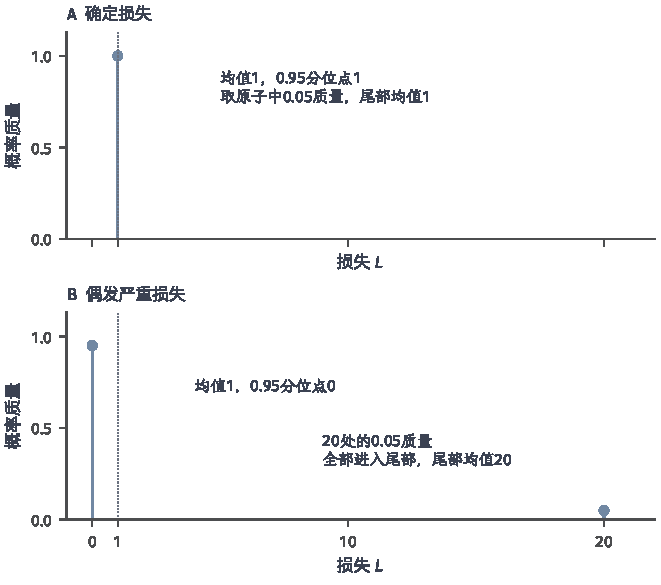
\includegraphics[width=112.000mm]{figures/10-reinforcement-learning/03-task-expansion-and-trustworthiness/matplotlib/rl-trustworthy-loss.pdf}
  \caption{两个教学损失分布，横轴为无量纲损失，纵轴为概率质量。粗实线和实心点表示原子，虚线标均值；图中文字说明用于计算CVaR的最差5\%质量，不是连续概率密度。}
  \label{fig:rl-trustworthy-loss}
\end{figure}

上面的定义假定损失分布已知。模型未知但允许运行当前策略时，可以直接用完整回合的样本估计累计损失，而不必先求转移核——因为我们只需要比较整个回合的后果，不需要知道每一步的转移核长什么样。设策略为$\pi_{\bm{\theta}}$，一回合损失为$L(\tau)$，把策略参数与尾部阈值组成联合目标
\[
  \Phi(\bm{\theta},\eta)
  =\eta+\frac{1}{1-\alpha}
      \mathbb E_{\tau\sim\pi_{\bm{\theta}}}(L(\tau)-\eta)_+.
\]
在环境不依赖策略参数、随机策略可微且支持不随参数突变，并能交换微分与期望的条件下，可用第~\ref{chap:rl-learning}~章的似然比方法求导。轨迹概率由逐步动作概率和环境转移概率相乘而成，环境项的参数导数为0，故其对数导数是
$\sum_{t=0}^{H-1}\nabla_{\bm{\theta}}\log\pi_{\bm{\theta}}(a_t\mid I_t)$。固定阈值，用超额损失加权这一轨迹得分，得到
\begin{equation}
  \nabla_{\bm{\theta}}\Phi
  =\frac{1}{1-\alpha}\mathbb E\left[
    (L-\eta)_+
    \sum_{t=0}^{H-1}\nabla_{\bm{\theta}}
       \log\pi_{\bm{\theta}}(a_t\mid I_t)\right].
  \label{eq:rl-trustworthy-tail-gradient}
\end{equation}
式~\eqref{eq:rl-trustworthy-tail-gradient}~中，未超过阈值的轨迹权重为0，超过阈值的轨迹按严重程度贡献策略更新。阈值本身的一个次梯度为
$1-(1-\alpha)^{-1}\mathbb P(L>\eta)$；在$L=\eta$处可以按$[0,1]$中的权重分配质量。算法~\ref{alg:rl-trustworthy-static-cvar}~据此同时更新阈值与策略，不需要把当前样本分位数当作真实分位数。

\begin{algorithm}[累计CVaR的轨迹更新]
  \label{alg:rl-trustworthy-static-cvar}
  \begin{algorithmic}[1]
    \Require 分位水平$\alpha$，时域$H$，批量$n$，步长序列，初值$\bm{\theta}^{(0)},\eta^{(0)}$
    \Ensure 候选策略及其阈值；可靠性另用留出评价样本验证
    \For{$k=0,\ldots,K-1$}
      \State 冻结当前参数，用$\pi_{\bm{\theta}^{(k)}}$独立启动$n$条轨迹，记录逐步损失并计算$L_j$
      \State 在旧参数、旧阈值上，用式~\eqref{eq:rl-trustworthy-tail-gradient}~的样本均值计算$\widehat{\bm{g}}_\theta$
      \State 计算$\widehat g_\eta=1-\frac{1}{n(1-\alpha)}\sum_j\mathbf 1\{L_j>\eta^{(k)}\}$，按需处理阈值处原子
      \State $\bm{\theta}^{(k+1)}=\bm{\theta}^{(k)}-\alpha_{\theta,k}\widehat{\bm{g}}_\theta$，
        $\eta^{(k+1)}=\eta^{(k)}-\zeta_k\widehat g_\eta$
    \EndFor
  \end{algorithmic}
\end{algorithm}

回到两条路线，可以直接检查梯度的行为含义。设出发时以概率$p=\operatorname{sigmoid}(\theta)$选偶发严重损失策略，否则选确定损失策略。对$0\leq p\leq1$，最差5\%质量由$0.05p$的损失20和$0.05(1-p)$的损失1组成，CVaR为$1+19p$。在$p=1/2$、最优阈值$\eta=1$处，精确策略梯度为$19p(1-p)=4.75$；沿负梯度更新会减小$\theta$，进而减少选择高尾部损失路线的概率。这个数由分布解析计算得到，不是训练实验的结果。

每批需要$nH$次交互与相应的策略求导，保存整批轨迹的空间也与$nH$成正比。经验分位数若通过排序求得，另需$O(n\log n)$；阈值次梯度只需$O(n)$。尾部估计还受有效回合数限制：用于最差部分的样本量约为$n(1-\alpha)$，这个数很小时，更新依赖极少数尾部回合，一整批也可能没有关键严重事件。误差还取决于损失尾部的大小及矩条件，不能只由这一回合数判断。

同批完整轨迹若既用于选择策略，又用于报告其尾部损失，还会引入选择偏差。模型轨迹能够减少真实交互，但模型在罕见区域的误差会直接影响尾部目标。百分位风险约束中的策略梯度和行动者--评论家方法同样需要估计风险、更新策略并调整约束，其局部收敛结论依赖特定假设；这些结论既不消除尾部估计误差，也不是任意神经网络训练的全局最优保证\scite{rl8-chow2018-percentile}

与无模型方法相对，已知有限时域模型时，也可以用动态规划求同一个静态目标，关键在于补齐状态。以累计损失
$L=\sum_{t=0}^{H-1}\gamma^t\ell_t$为例，只保存物理状态无法知道终点的超额损失，因而再记录已经积累的损失$z$。先固定出发前选定的$\eta$，把终端目标设为$(z-\eta)_+$，再用普通期望向后递推：
\begin{align}
  W_H^\eta(s,z)&=(z-\eta)_+, \nonumber\\
  W_t^\eta(s,z)&=\min_{a\in\mathsf A(s)}
       \mathbb E\!\left[
       W_{t+1}^\eta(s',z+\gamma^t\ell_t)\mid s,a\right].
  \label{eq:rl-trustworthy-augmented-risk}
\end{align}
再在出发前最小化
$\eta+(1-\alpha)^{-1}\mathbb E_{s_0\sim\mu_0}W_0^\eta(s_0,0)$。
每步把$\gamma^t\ell_t$加到累计量中，模型期望同时覆盖后继状态与本步损失；策略因此可以依赖时间、状态和已观察的累计损失。损失支持离散且有限时，可枚举可达$z$；$z$连续时，离散化或插值会扩大状态规模并引入误差。阈值仍属于事前承诺，途中重置为新的条件分位数会改变目标。另有增广方法保存尾部概率预算；原论文以尾部质量为参数，换成本章记号时应使用$1-\alpha$\scite{rl8-chow2015-cvar}

\begin{example}[静态CVaR的时间不一致]
  \label{ex:rl-trustworthy-time-inconsistency}
  设$H=2$且不折扣。$t=0$只有一个虚拟动作，损失为0，随后进入可观察的分支A或B，概率分别为0.1与0.9。$t=1$在B只有一个动作，损失固定为10；在A可以选safe，损失12，也可以选risky，损失以0.9概率为0、以0.1概率为20。决策者在$t=0$选择并承诺一个完整条件策略，在到达A后执行约定动作。

  取$\alpha=0.9$。承诺safe时，总损失分布为$10(0.9),12(0.1)$，CVaR为12。承诺risky时，分布为$0(0.09),10(0.9),20(0.01)$，最坏10\%由全部1\%的20和9\%的10组成，所以
  \[
    \operatorname{CVaR}_{0.9}(L_{\text{risky}})
       =\frac{0.01\times20+0.09\times10}{0.1}=11.
  \]
  事前准则严格选择risky。但一旦到达A，重新最小化条件CVaR，safe与risky的数值分别为12与20，因而严格选择safe。环境和可选动作没有改变，改变的是条件化之后用于定义尾部的概率质量。
\end{example}

反例中分支已被观察，冲突仍然发生：到达A后，定义最差10\%时不再计入B的概率质量。静态CVaR若只在原物理状态上套用普通Bellman递推，就可能丢掉事前评价的这层含义。式~\eqref{eq:rl-trustworthy-augmented-risk}~通过累计损失和固定阈值保留事前目标；若任务反而要求每个历史下都按当前条件重新评价，则需要下一小节的动态目标。

% Outline: 8.2.2
\subsection{逐阶段条件风险下的决策}
\label{sec:rl-trustworthy-dynamic-risk}

静态准则的时间不一致反例提示了另一种决策观：如果决策者不打算事先承诺，而是保留在每次取得新的观测、奖励或损失记录后重新决策的权利，就需要逐阶段地评价风险。到达A后，B已经被排除，未来方案可以只按A下的后果比较。\term{条件风险映射}（conditional risk mapping）执行的就是这一步：把下一阶段的不确定损失汇总成以当前已揭示记录为条件的风险数值。该数值在当前历史下已知，在更早时刻却仍可能随机。令$\mathcal F_t$为截至时刻$t$已揭示的状态或观测、已执行动作及已到达奖励或损失记录生成的$\sigma$代数；协议额外给出的公共信号也一并纳入。映射$\rho_t$把$\mathcal F_{t+1}$可测损失变成$\mathcal F_t$可测量。条件CVaR在式~\eqref{eq:rl-trustworthy-cvar}~中改用$\mathbb E[\cdot\mid\mathcal F_t]$，阈值也改为$\mathcal F_t$可测的随机变量；一般概率空间上使用本质下确界，即忽略零概率集合后仍成立的最大下界。有限树上，这等于在每个正概率历史的条件分布内分别优化阈值。不同策略的风险各自按其诱导分布计算；要比较这种排序能否跨时刻保持，则须在同一概率空间及同一组按时刻递增的$\sigma$代数下进行，不将不同策略的两条轨迹直接逐点配对。这样的几乎处处结论也不自动覆盖运行分布未支持的历史。

为将条件风险用于逐阶段交互控制，固定正整数时域$H$、$0\leq\gamma\leq1$、概率空间$(\Omega,\mathcal F,\mathbb P)$及递增$\sigma$代数族$\mathcal F_0\subseteq\cdots\subseteq\mathcal F_H$。令$L^\infty(\mathcal F_t)$表示相对于$\mathbb P$几乎处处有界、在$\mathcal F_t$下可测的随机变量。
  取归一化$\rho_t(0)=0$的一步条件风险映射$\rho_t:L^\infty(\mathcal F_{t+1})\to L^\infty(\mathcal F_t)$。对阶段损失$\ell_t\in L^\infty(\mathcal F_{t+1})$，定义
  \[
    \mathcal R_t
      =\rho_t(\ell_t+\gamma\mathcal R_{t+1}),
      \qquad \mathcal R_H=0.
  \]
  这一递归是\term{嵌套风险}（nested risk），即把后一步风险当作当前待评价的未来损失。
  动态风险族具有\term{时间一致性}（time consistency），如果对任意$0\leq u<v\leq H$和上述同一空间上的两个损失序列，它们在$u,\ldots,v-1$几乎处处相同，且$v$时刻的条件风险几乎处处满足$\mathcal R_v\leq\widetilde{\mathcal R}_v$，就有
  $\mathcal R_u\leq\widetilde{\mathcal R}_u$。
  所有几乎处处比较均相对于同一个$\mathbb P$。有界空间使逐层输入和输出仍在映射定义域内；无界损失的动态风险须另给可积性与定义域封闭条件，不能只沿用静态CVaR的可积假设。

共同概率空间可以先按一棵固定的随机树理解：分支、分支概率和前段损失不变，只比较两套后续损失。例如两个叶节点上的损失分别为$X=(2,4)$与$Y=(3,5)$，就能在同一叶节点逐项比较$X\leq Y$；单调的条件风险把这种排序逐层向前传递。这里检查的是同一条件风险规则怎样评价不同损失，并不是把两个机器人各自运行得到的轨迹强行配对。

控制优化还要加入动作对后继分布的影响。不同动作可以产生不同的下一状态分布，因而下面分别用$\rho_{t,s,a}$表示给定状态动作后的一步条件风险。先按每个动作对应的条件分布计算风险，再比较动作，与前面的共同空间排序性质并不冲突。

时间一致性保留跨时刻的排序：两方案前段损失相同，若以后在每个可能历史下一个方案的条件风险都不更高，较早评价也不应把它排得更差。各$\rho_t$单调时，将$v$时刻的不等式逐层代入递归，就能传到$u$。这一论证控制的是条件风险排序，并未断言每条轨迹都没有损失。动态风险及其Markov表示的系统论述见原始工作\scite{rl8-ruszczynski2010-risk}

在示例~\ref{ex:rl-trustworthy-time-inconsistency}~中，每层采用$\alpha=0.9$的条件CVaR。先在A内汇总叶节点，risky得到20，safe得到12；B的风险为10。再汇总分支风险$20(0.1),10(0.9)$，risky的嵌套风险为20，safe则为12。图~\ref{fig:rl-trustworthy-risk-tree}~对照这两种运算：静态准则直接使用叶节点的联合概率，嵌套准则先把分支后果压成条件风险。选择从risky变为safe，来自评价对象改变，而非静态求解精度提高。

\begin{figure*}[t]
  \centering
  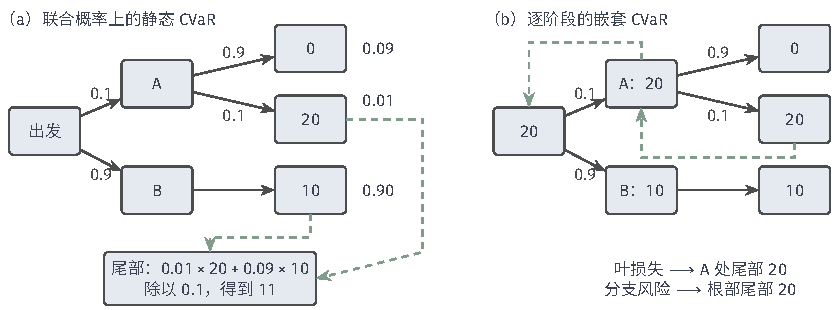
\includegraphics[width=141.390mm]{figures/10-reinforcement-learning/03-task-expansion-and-trustworthiness/tikz/rl-trustworthy-risk-tree.pdf}
  \caption{同一教学决策树的两种风险汇总，均取$\alpha=0.9$、$H=2$且不折扣。图中展示承诺risky的分支；实线表示随机转移，带文字的回传箭头表示风险计算。safe只需将A的两个叶节点替换为固定损失12。}
  \label{fig:rl-trustworthy-risk-tree}
\end{figure*}

分支树可以逐层回传，状态价值递推却还要求状态保存决定后继条件分布和风险映射的历史记录、累计损失或剩余预算。这里要求给定$(t,s,a)$后，后继条件分布、风险映射及其水平不再依赖未记录的历史；各映射在相应条件分布的有界后继变量上定义，并满足单调性，使后续风险的改善能够传到当前评价。设动作确定后，一步损失$\ell(s,a)$已知，$\rho_{s,a}$只评价后继状态上的随机量。若风险满足平移等变性，即加上当前已知常数会使风险增加同一常数，就能把这一步损失移到映射外。有限时域Markov风险问题于是可向后归纳为
\begin{equation}
  V_t(s)=\min_{a\in\mathsf A(s)}
    \{\ell_t(s,a)+\rho_{t,s,a}(\gamma V_{t+1}(s'))\},
  \qquad V_H=0.
  \label{eq:rl-trustworthy-risk-bellman}
\end{equation}
式~\eqref{eq:rl-trustworthy-risk-bellman}~先评价每个动作下的未来风险，再选损失风险最小的动作。一步损失若也随机，须将$\ell_t+\gamma V_{t+1}$一起放入联合分布的风险映射；风险水平若依赖剩余预算或历史，相应的剩余预算或历史记录也须进入状态。这里采用确定性Markov动作选择。允许随机动作时，还要规定风险在随机化之前还是之后评价，否则算子所优化的目标并未确定。

\begin{theorem}[折扣风险算子的压缩性]
  \label{thm:rl-trustworthy-risk-contraction}
  设状态集$S$及每个可行动作集$\mathsf A(s)$有限且非空，确定阶段损失$\ell(s,a)$有界，$0<\gamma<1$。对每个$(s,a)$，固定后继条件分布及风险规则，映射$\rho_{s,a}:\mathbb R^{|S|}\to\mathbb R$在所有有限后继值向量上有定义，迭代中不改变；所需历史已计入状态。
  每个映射满足单调性，即逐后继状态$X\leq Y$推出$\rho_{s,a}(X)\leq\rho_{s,a}(Y)$，并对任意实常数$b$满足平移等变性
  $\rho_{s,a}(X+b)=\rho_{s,a}(X)+b$。
  对已经按声明的风险问题建立的算子
  \[
    (\mathcal B V)(s)=\min_{a\in\mathsf A(s)}\{\ell(s,a)+\rho_{s,a}(\gamma V(s'))\},
  \]
  对任意$V,W\in\mathbb R^{|S|}$，有$\lVert\mathcal B V-\mathcal B W\rVert_\infty\leq\gamma\lVert V-W\rVert_\infty$。
  因而该算子有唯一不动点，反复应用$\mathcal B$从任意有限初值收敛到该点。
\end{theorem}
\begin{proof}
  令$\varepsilon=\lVert V-W\rVert_\infty$。对所有后继状态，
  $\gamma W-\gamma\varepsilon\leq\gamma V\leq\gamma W+\gamma\varepsilon$。
  单调性把不等式传入$\rho_{s,a}$，平移等变性把两端的常数移出，得到
  \[
    \rho_{s,a}(\gamma W)-\gamma\varepsilon
      \leq\rho_{s,a}(\gamma V)
      \leq\rho_{s,a}(\gamma W)+\gamma\varepsilon.
  \]
  记每个动作的花括号表达式为$q_V(s,a)$和$q_W(s,a)$，则
  $|q_V-q_W|\leq\gamma\varepsilon$。对所有动作的下界取最小值，得
  $(\mathcal B V)(s)\geq(\mathcal B W)(s)-\gamma\varepsilon$；取上界的最小值，得反向界。因此所需无穷范数界成立。

  $\mathbb R^{|S|}$配无穷范数是非空完备度量空间，上述算子把它映回自身，且压缩因子为$\gamma<1$。压缩不动点结论因此给出唯一不动点及任意有限初值的几何收敛，并有
  $\lVert V^{(k)}-V^\star\rVert_\infty\leq\gamma^k\lVert V^{(0)}-V^\star\rVert_\infty$。
  相关基础可参考\BookChapterRef{chap:metric-spaces}{卷1《数学准备：计算、分析与几何》“度量空间”章}。这里保证的是已经按声明风险建立的固定算子的求解，不保证环境或风险模型本身正确。
\end{proof}

证明用单调性传递上下界，用平移等变性移出误差常数，没有使用正齐次性，因而将折扣留在$\rho(\gamma V)$内部即可。它回答的是价值迭代是否收敛。不动点是否代表希望求解的风险目标，还须核对时间一致性、状态所保存的历史与预算和允许策略类，数值压缩性本身不证明这些建模条件。

以已知有限模型的条件CVaR价值迭代为例，每轮先冻结$V^{(k)}$。对每个$(s,a)$，列出后继值$\gamma V^{(k)}(s')$及概率，按值排序并从最大值累计$1-\alpha$质量，再由式~\eqref{eq:rl-trustworthy-tail-mass}~求风险；加上$\ell(s,a)$后，对动作取最小值。排序是在寻找严重损失尾部，动作最小化则是在改善决策。迭代到残差
$\lVert\mathcal B V^{(k)}-V^{(k)}\rVert_\infty\leq(1-\gamma)\epsilon$时，
压缩界与三角不等式给出
$\lVert V^{(k)}-V^\star\rVert_\infty\leq\epsilon$。
在两阶段树上，从终端0开始，A的回传立即得到$\min(12,20)=12$，B得到10，根部再得到12，完成一次可复核的向后计算。

记状态数为$m$、每状态最多$b$个动作，稠密转移下每轮排序更新需$O(bm^2\log m)$，模型存储需$O(bm^2)$。若只有指定状态动作的采样接口，就需用独立后继批次估计条件分布；条件CVaR是分布的非线性函数，单个后继样本的风险一般不能无偏估计总体风险。每步近似算子误差若一致不超过$e$，迭代误差满足
$\Delta_{k+1}\leq\gamma\Delta_k+e$，长期误差上限为$e/(1-\gamma)$。
因此，风险策略梯度需要与嵌套目标相符的风险权重，分布评论家则需估计相应的条件后果分布。把期望评论家的价值预测换成尾部分位数，只改变了一个预测量；还须推导它如何参与目标和更新，才能得到所声明的风险算法。

% Outline: 8.3
\section{不确定环境下的鲁棒决策}
\label{sec:rl-trustworthy-robust}

风险准则处理的是一个固定概率模型内部的随机性。现在放宽“模型已知且准确”这个前提：部署环境可能与训练时不同，问题转为同一策略能否在允许的变化范围内维持要求。注意这里不假设各环境以某个概率出现——工程师通常只知道摩擦的物理区间、传感器的误差规格，而不知道“今天是干地还是湿地”的概率，因此不能简单取期望，只能保证整个范围内的最坏表现。变化进入系统的位置不同，应对手段也不同。图~\ref{fig:rl-trustworthy-channels}~固定交互闭环，区分三个扰动位置：摩擦变化影响真实状态转移，传感读数修改影响策略读取的观测，制动力削弱影响请求动作的实际执行。对抗训练是在这些位置搜索不利变化的求解手段，不是第四种扰动对象。

\begin{figure*}[t]
  \centering
  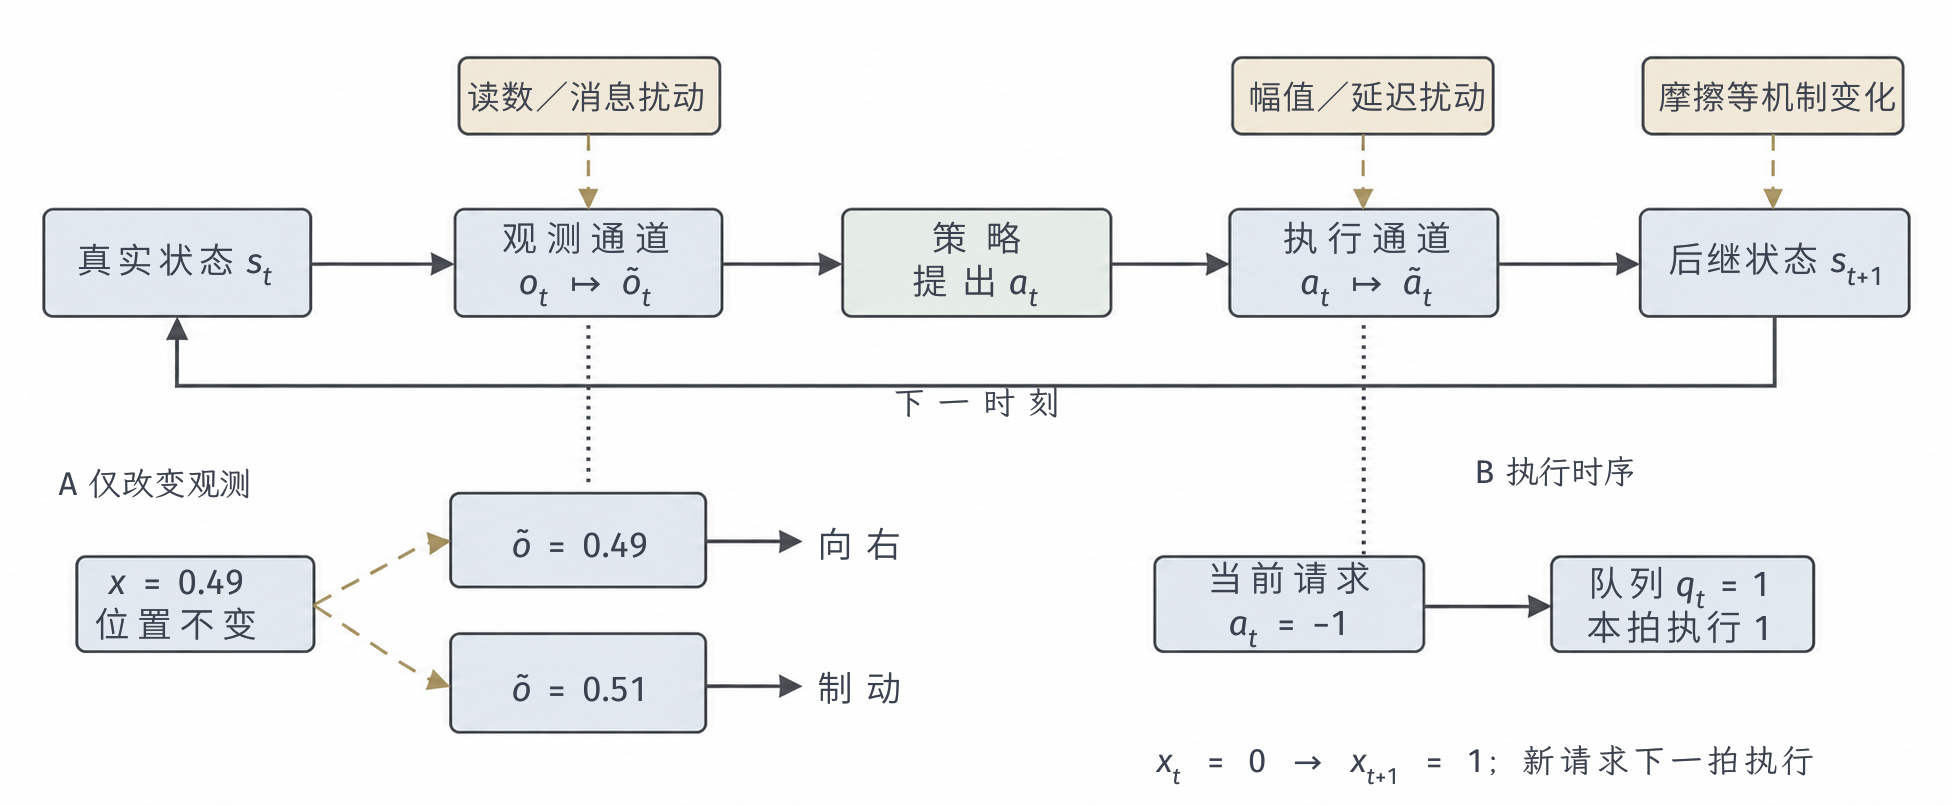
\includegraphics[width=157.400mm]{figures/10-reinforcement-learning/03-task-expansion-and-trustworthiness/generated/rl-trustworthy-channels/figure.png}
  \caption{扰动进入交互闭环的三个位置。实线传递状态、观测与动作，虚线表示不同扰动权限。下方两个局部面板分别只突出观测误差和执行延迟，二者均不等于直接改变当前真实位置。点状引线只定位下方对应通道的局部示意，不表示额外运行路径。}
  \label{fig:rl-trustworthy-channels}
\end{figure*}

% Outline: 8.3.1
\subsection{环境机制变化下的鲁棒决策}
\label{sec:rl-trustworthy-mechanism}

先处理动力学本身的不确定性。摩擦系数的点估计0.6给出标称模型$\widehat T$，用它规划相当于赌真实摩擦恰好是0.6；物理测量若只支持区间$[0.4,0.8]$，则给出一族可能转移核$\mathcal U$，鲁棒规划要在这一族上都站得住。前者适合预测标称表现，后者适合检查整个允许范围内的不利表现。固定奖励$R$和初态分布$\mu_0$，只让转移核变化，从而单独识别动力学不确定性的影响。区间没有规定各模型出现的概率，因而尚不能对模型作概率平均；即使另给概率权重，平均回报较高也可能掩盖某个允许模型下的低回报。要为集合内每个模型提供统一下界，就先对同一策略取回报的下确界，再选择这个下界最大的策略；每个模型内部的随机轨迹仍由$J_T(\pi)$取期望。

\begin{definition}[最坏情形回报]
  \label{def:rl-trustworthy-robust-return}
  固定有限状态动作、非空可行动作、有界奖励$R$、初态分布$\mu_0$和$0\leq\gamma<1$。令$\mathcal U$为非空允许转移核集合，各核均给出每个状态动作下的概率分布；$J_T(\pi)$是在核$T$下由$\mu_0$启动、按策略$\pi$运行的期望折扣回报。给定非空合法候选策略类$\Pi$，其中每条策略均按其获准历史选择合法动作。对固定$\pi\in\Pi$，鲁棒回报及该类中的最优值为
  \[
    J_{\mathrm{rob}}(\pi)=\inf_{T\in\mathcal U}J_T(\pi),
    \qquad J_{\mathrm{rob}}^\star=\sup_{\pi\in\Pi}J_{\mathrm{rob}}(\pi).
  \]
  集合$\mathcal U$描述允许的环境，而不是轨迹中随机转移结果的集合。若奖励或初态也不确定，应把它们与$T$一起列入模型集合。
  候选类$\Pi$还须指定允许确定性、随机化和历史依赖的范围。最优值能否由某条策略取到需另证；保证取到以后，才可把上确界写成最大值。
\end{definition}

区间可以来自设备的物理界，也可以来自转移记录的联合置信区域；两种来源的保证不同。若$\mathcal U=\mathcal U(D)$由转移记录$D$构造，模型假设还需附带统计覆盖事件
$\{T_{\text{真}}\in\mathcal U(D)\}$。在该事件上，任何被评价策略都有
$J_{T_{\text{真}}}(\pi)\geq\inf_{T\in\mathcal U}J_T(\pi)$。
这是集合内的确定性比较：真实模型只要被包含，最坏回报便是其回报下界。集合若以至少$1-\delta$的概率覆盖真实模型，才能进一步形成带置信水平的声明。集合过小可能漏掉真实环境，过大则可能降低可保证的回报，付出不必要的保守代价。鲁棒MDP需要同时说明集合结构和转移记录所给出的置信区域\scite{rl8-wiesemann2013-robust}

最坏回报定义是对整个模型一次性取最坏，但Bellman备份每次只处理一个状态动作；要让局部选择拼出一个合法的全局最坏环境，集合还须能够分解。\term{状态--动作矩形性}（state-action rectangularity）指
$\mathcal U=\prod_{s,a}\mathcal U_{s,a}$，也就是从各局部集合任选一个转移分布，组合后仍是允许模型。相应动态对手看到当前状态和已选动作后，在$\mathcal U_{s,a}$中选择下一步分布，不受跨状态或跨时间的共享剩余预算约束。下面采用最小值写法时，还要求各$\mathcal U_{s,a}$是概率单纯形中的非空紧集，使连续的线性目标能够取到最小值；若只知道局部集合非空而不能保证取到，则应把内层写成下确界。按这些条件与权限得到
\begin{equation}
  (\mathcal B_{\mathrm{rob}}V)(s)
    =\max_{a\in\mathsf A(s)}
      \left\{R(s,a)+\gamma
        \min_{p\in\mathcal U_{s,a}}\sum_{s'}p(s')V(s')\right\}.
  \label{eq:rl-trustworthy-robust-bellman}
\end{equation}
式~\eqref{eq:rl-trustworthy-robust-bellman}~的外层最大化回报，内层最小化给定动作下的后继价值。先选动作再让对手选择分布，正是前述对手读取当前状态与动作的权限；若对手须在看到动作前承诺一个跨动作共享的参数，允许的局部选择会变少，不能直接沿用同一算子。

\begin{theorem}[矩形鲁棒Bellman算子的压缩性]
  \label{thm:rl-trustworthy-robust-contraction}
  设状态集$S$及可行动作集$\mathsf A(s)$有限且非空，奖励$R(s,a)$有界，$0<\gamma<1$，每个$\mathcal U_{s,a}$都是$S$上概率单纯形中的非空紧集。令全局转移核集合为$\mathcal U=\prod_{s,a}\mathcal U_{s,a}$，对手在当前状态和动作已知后选择本步分布，不受跨步共享约束；状态是双方所用历史的共同充分表示。固定这些奖励、集合与权限后，式~\eqref{eq:rl-trustworthy-robust-bellman}~作为$\mathbb R^{|S|}$上的算子，在无穷范数下是$\gamma$压缩映射。
\end{theorem}
\begin{proof}
  令$\varepsilon=\lVert V-W\rVert_\infty$。对任意概率向量$p$，
  \[
    \left|\sum_{s'}p(s')V(s')-\sum_{s'}p(s')W(s')\right|
      \leq\sum_{s'}p(s')\varepsilon=\varepsilon.
  \]
  记内层最小值为$m_V,m_W$。上式对集合中每个$p$都成立，故
  $\sum pV\geq\sum pW-\varepsilon\geq m_W-\varepsilon$，取最小值得
  $m_V\geq m_W-\varepsilon$。由于紧性保证$W$的最小点$p_W$存在，
  $m_V\leq\sum p_WV\leq m_W+\varepsilon$。于是$|m_V-m_W|\leq\varepsilon$。
  加入相同的$R(s,a)$并乘以$\gamma$，每个动作的表达式相差至多$\gamma\varepsilon$。
  对各动作的上下界分别取最大值，得到
  \[
    (\mathcal B_{\mathrm{rob}}W)(s)-\gamma\varepsilon
      \leq(\mathcal B_{\mathrm{rob}}V)(s)
      \leq(\mathcal B_{\mathrm{rob}}W)(s)+\gamma\varepsilon.
  \]
  对状态取最大绝对差，结论成立。不动点存在、唯一及价值迭代收敛，由定理~\ref{thm:rl-trustworthy-risk-contraction}~中使用的非空完备空间上的压缩不动点结论得到。
\end{proof}

压缩证明控制的是数值迭代，矩形性则把局部最坏选择接成合法的全局环境。不动点处，各状态可取一个外层最优动作，各状态动作可取一个内层最差分布；由于这些分布可自由组合，它们共同给出$T^\star\in\mathcal U$。固定平稳Markov策略时，将外层最大化换成按$\pi(a\mid s)$平均，保留各动作下的内层最小化，就得到该策略在矩形模型族中的最坏回报评价。

历史依赖策略还需在状态中保留所用记忆，但状态增广不自动产生矩形性。若以$(s,m)$表示物理状态与记忆，同一个物理参数在不同记忆副本间共享的关系仍须保留；不能仅因$m$不同，就允许对手分别选择彼此不相容的参数。否则得到的是更大的不确定集合，后面的共享参数示例~\ref{ex:rl-trustworthy-coupling}~说明了这种扩大怎样改变最坏回报。局部备份与动态对手的对应，由有限时域逐步归纳和无限时域折扣极限建立；有限时域模型族还须允许各时刻局部分布独立组合。空间上的矩形性并不自动赋予时间上的自由变化，任意耦合集合也不满足这套分解条件。

求解式~\eqref{eq:rl-trustworthy-robust-bellman}~时，置信多面体使内层成为线性目标$\sum pV$的线性规划；只有两个后继状态的概率区间时，线性目标在端点取最小值。教学例取后继价值10与0、$\gamma=0.9$、当前奖励0，好状态概率$p\in[0.7,0.9]$。最坏选择为$p=0.7$，备份为$0.9\times0.7\times10=6.3$；标称$p=0.8$时为7.2。另一动作若确定到达价值7.5的后继，其备份为6.75，于是标称选择第一个动作，鲁棒选择第二个动作。

每轮冻结旧价值，逐状态动作求内层最小值，再取外层最大值。记一次内层优化代价为$C_{\text{内}}$，每轮需$O(mbC_{\text{内}})$。内层求解残差、模型集合估计误差和价值逼近误差影响不同步骤，应分别记录，不能只报告最终迭代残差。

\begin{example}[共享参数不能随状态独立取坏值]
  \label{ex:rl-trustworthy-coupling}
  一个两阶段教学任务以相同概率从$s_1,s_2$启动，各只有一个动作，第一步奖励0。下一步到达成功状态得到奖励1，失败状态得到0，随后终止。整个环境共享一个固定未知参数$\vartheta\in[0,1]$，成功概率分别是
  $p_1=\vartheta$与$p_2=1-\vartheta$。
  对任意合法环境，初态平均回报都为
  $\gamma(p_1+p_2)/2=\gamma/2$。
  如果只保留每个概率各自属于$[0,1]$，逐状态最坏选择会取$p_1=p_2=0$，得到回报0；然而不存在同时产生这两个概率的$\vartheta$。
\end{example}

图~\ref{fig:rl-trustworthy-rectangular}~的斜线给出共享参数真正允许的组合，方形则允许局部概率各自取坏值。扩大集合的算子即使严格收敛，也是在解更保守的另一个问题。共享参数若能由历史观测逐渐识别，新观测还可能通过辨识共享参数来改善后续控制；保留参数信念或相关历史才能利用它，将每次访问都当作对手重新任意选参数会丢掉这一机会。

\begin{figure}[htbp]
  \centering
  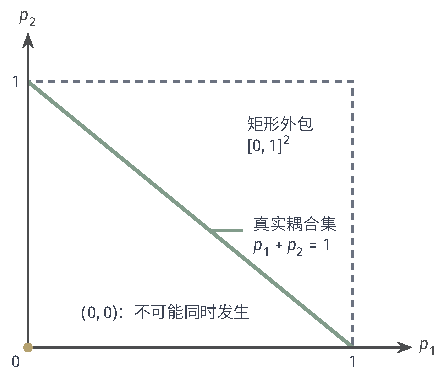
\includegraphics[width=75.805mm]{figures/10-reinforcement-learning/03-task-expansion-and-trustworthiness/tikz/rl-trustworthy-rectangular.pdf}
  \caption{教学耦合集$\{(p_1,p_2):p_1+p_2=1\}$与矩形外包$[0,1]^2$。方形左下角给出局部最坏选择，却不属于共享参数模型。坐标是两状态的成功概率。}
  \label{fig:rl-trustworthy-rectangular}
\end{figure}

“分布鲁棒”仍须说明哪个分布不确定。可能变化的是后继状态转移分布$p(\cdot\mid s,a)$，也可能是随机环境参数$\vartheta$的分布$\nu$；后一种问题优化
$\inf_{\nu\in\mathfrak U}\mathbb E_{\vartheta\sim\nu}J_{T_\vartheta}(\pi)$。
回合开始时抽取模型并保持不变，会使整段轨迹共享参数；每步重新抽取通常产生不同过程。Xu与Mannor的分布鲁棒MDP用参数分布的嵌套集合约束表示已知的参数概率或概率界，并建立相应状态分解与求解条件；这些条件不是把任意参数分布歧义集逐状态拆开的许可\scite{rl8-xu2010-distributional}

表~\ref{tab:rl-trustworthy-uncertainty}~按不确定对象对齐集合来源和求解条件。其他参与者造成的转移变化，还须符合第~\ref{chap:rl-multi-agent}~章的联合行为模型，不能擅自赋予其任意局部变化权限；识别未知参数后再适应，则涉及第~\ref{chap:rl-transfer}~章的任务推断。

\begin{table}[htbp]
  \centering
  \begin{tabularx}{\linewidth}{@{}>{\raggedright\arraybackslash}p{20mm}XX@{}}
    \toprule
    不确定对象 & 集合来源与矩形条件 & 内层求解及保证范围 \\
    \midrule
    参数$\vartheta\in\Theta$ & 物理区间或联合置信集；共享参数通常耦合状态 & 在$\Theta$上优化；覆盖整个参数族，不自动支持局部备份 \\
    转移分布$p\in\mathcal U_{s,a}$ & 距离球、矩或似然约束；须说明各对之间能否自由组合 & 线性、凸或专门分布优化；只覆盖声明集合 \\
    参数分布$\nu\in\mathfrak U$ & 对模型参数随机性的矩、支持或概率质量约束 & 对分布求最坏期望；需说明参数抽取时机及依赖 \\
    \bottomrule
  \end{tabularx}
  \caption{三种不同层次的不确定性。置信覆盖是构造集合的额外统计性质，不由“鲁棒”或“分布鲁棒”的名称保证。}
  \label{tab:rl-trustworthy-uncertainty}
\end{table}

% Outline: 8.3.2
\subsection{观测信息受扰下的鲁棒决策}
\label{sec:rl-trustworthy-observation}

第二类扰动不改动物理世界，而在机器人感知世界的读数上做手脚——这对应传感器误差或针对感知的攻击。摩擦模型的不确定性已经明确，下面固定真实动力学与路线，只改变传感器报告。记真实状态为$s_t$，原始观测为$o_t$，受扰观测为$\widetilde o_t$，策略能够使用的历史为
$\widetilde I_t=(\widetilde o_0,a_0,\ldots,\widetilde o_t)$。
为确定最坏情形，先声明威胁模型，也就是扰动者的修改范围与观测、策略参数和历史读取权限。例如传感器误差规格给出$\epsilon$，扰动者在原始观测产生后、策略采样动作前选择
$\widetilde o_t\in\mathcal B_\epsilon(o_t)=\{o:\lVert o-o_t\rVert_\infty\leq\epsilon\}$；
它能看到当前原始观测和策略参数，不能看到未来噪声或尚未采样的动作。总预算若还满足$\sum_t\lVert\widetilde o_t-o_t\rVert\leq B$，先前修改会消耗后续权限，剩余预算便须进入对手状态。逐步误差界与整回合预算约束不同，两者产生的最坏情形也不同。

图~\ref{fig:rl-trustworthy-channels}~的观测面板固定真实位置$x=0.49$。教学策略在读数小于0.5时向右，否则制动；读数0.49与0.51都满足$|\widetilde o-x|\leq0.02$，却触发不同动作。机器人没有因此移动到0.51，变化只发生在策略读取的观测。若测试只覆盖$\widetilde o=0.48,0.49$，就没有触及允许集合另一侧的动作切换；两个测试通过不足以覆盖整个误差范围。

训练时，可以先冻结当前策略，在允许预算内搜索使回报降低的观测序列，再用受扰轨迹更新策略，最后以未参与更新的扰动规则和启动条件检验。令$\iota_t$表示威胁模型允许扰动者在时刻$t$读取的观测、策略参数与历史记录；在上述示例中，它只能由当前原始观测、策略参数以及协议明确允许的记录组成。以无记忆确定性连续动作策略为例，若有只依赖$\iota_t$与动作的可微一步价值代理，可从$o_t$初始化并进行投影梯度搜索：
\[
  \widetilde o^{(j+1)}
   =\operatorname{Proj}_{\mathcal B_\epsilon(o_t)}
      \left(\widetilde o^{(j)}
       -\xi\nabla_{\widetilde o}
          \widehat Q(\iota_t,\pi_{\bm{\theta}}(\widetilde o^{(j)}))\right).
\]
这里$\xi>0$是搜索步长，$\widehat Q$按奖励回报计分。负梯度搜索以降低这一代理价值为目标，投影使修改后的观测仍在允许误差集合内；步长与代理光滑性不合适时，单步也未必降低目标。该式只处理逐步误差球，若另有整回合预算，还须限制本步支出并更新剩余预算。模拟训练若额外把真实状态$s_t$输入评论家，就属于特权训练：只有$s_t$能由$\iota_t$确定，或最终扰动规则已经去除特权输入并能仅凭$\iota_t$执行时，该规则才属于上述威胁模型的允许集合；否则它评价的是允许读取额外真实状态或历史的另一威胁模型，不能充当前允许规则的攻击证据。无论依据哪些允许读取的观测或记录，投影搜索都只是在局部代理上寻找不利观测，没有保证整条轨迹最坏。随机策略须对动作分布下的期望价值求导，不能把分布本身当作动作输入$\widehat Q$；有记忆策略则须把协议允许的受扰历史纳入$\iota_t$，并保留它对策略内部状态的影响。

生成受扰样本后，可用第~\ref{chap:rl-learning}~章的策略更新提高受扰回报。更新后的参数又改变下一轮攻击目标，因此对手梯度与策略梯度须分开计算。每步若搜索$K_{\text{攻}}$次，梯度计算代价约增为普通采样的该倍数；增加搜索量也不等于证明搜索完备。

除了受扰训练，还可以减少观测所对应的状态歧义。鲁棒状态估计将读数转成与误差模型相容的状态集合，历史方法借助动力学和多次观测排除部分状态，观测保护则修复或拒绝可疑读数。它们分别依赖有效误差界、足够准确的动力学或可识别的异常观测。

修复器输出$\widehat o$若仍有误差$\|\widehat o-o\|\leq e$，要将它传到行为上，还需确定性连续动作策略在该区域满足Lipschitz条件，即观测距离能按固定比例控制动作距离。此时
$\|\pi(\widehat o)-\pi(o)\|\leq L_\pi e$；进一步得到回报或安全界，还需价值或闭环动力学的敏感性界。前述阈值策略在切换面附近不满足这种连续性估计。信念与历史状态的构造见第~\ref{chap:rl-information}~章。

把满足前述修改范围、可读观测与记录及预算的整回合扰动规则组成集合$\mathcal N$，以$\nu$表示其中一条规则；此处$\nu$不是上一小节的参数分布。固定策略与规则后，$J(\pi,\nu)$是在其诱导轨迹分布下的期望回报，定义真实最坏回报$J_{\min}=\inf_{\nu\in\mathcal N}J(\pi,\nu)$。近似搜索若找到允许规则$\widehat\nu\in\mathcal N$，则
$J_{\min}\leq J(\pi,\widehat\nu)$：该规则的期望回报对最坏回报只是一个上界，单次攻击样本或有限样本均值却不必满足这一确定性比较。只有另外证明内层误差
$J(\pi,\widehat\nu)-J_{\min}\leq e_{\text{攻}}$，才能得到
$J_{\min}\geq J(\pi,\widehat\nu)-e_{\text{攻}}$。
若期望回报也由样本估计，所得下界还须扣除相应统计误差。近似攻击只找到允许集合中的一个候选，其他扰动可能更坏。覆盖全部允许的观测扰动规则，仍需搜索完备性、可验证的内层误差界或形式化分析；若干攻击下表现良好只支持已测条件下的结论。

% Outline: 8.3.3
\subsection{动作执行受扰下的鲁棒决策}
\label{sec:rl-trustworthy-actuation}

第三个扰动位置在感知之后、物理世界之前：执行机构。前两小节默认“策略决定的动作会被精确执行”，但真实的电机和刹车都有幅值误差、饱和与延迟。即使观测准确，策略请求制动也不意味着制动力立即足量施加。记请求动作为$a_t$，实际动作为$\widetilde a_t$。幅值误差可写成$\widetilde a_t=a_t+e_t$、$\|e_t\|\leq\epsilon_a$，其中$\epsilon_a$来自执行器误差规格；若有饱和，还须把实际动作限制在设备能力内。动作篡改须声明攻击者何时读取请求，延迟须声明队列和最大滞后。图~\ref{fig:rl-trustworthy-channels}~的执行面板区分了请求与实际动作。

固定一拍延迟时，下一步执行的是旧请求，物理系统满足
$x_{t+1}=f(x_t,a_{t-1},w_t)$。当前状态$x_t$和请求$a_t$不足以确定下一步分布，还须知道队列内容。把它记为$q_t=a_{t-1}$并增广状态
$z_t=(x_t,q_t)$，得到
\begin{equation}
  x_{t+1}=f(x_t,q_t,w_t),\qquad q_{t+1}=a_t.
  \label{eq:rl-trustworthy-delay}
\end{equation}
若$w_t$在给定$z_t,a_t$后由固定核抽取，增广状态就恢复了马尔可夫转移。教学系统$x_{t+1}=x_t+\widetilde a_t$在$x_t=0,q_t=1$时，即使请求$a_t=-1$，下一步仍到$x_{t+1}=1$；新请求只将队列改为$-1$。省略队列会遗漏真正决定本步运动的动作，进而误判制动请求的效果。

执行误差集合已知时，应对每个请求动作评价其可能的实际效果。以回报价值$V$为例，集合只规定允许的执行误差，没有给这些误差的概率权重；要覆盖集合中每种误差，就取后继期望价值的下确界，而不能用若干误差的平均值代替。内层最坏后继价值为
\begin{equation}
  \inf_{e\in E(s,a)}
       \mathbb E\!\left[V\bigl(f(s,a+e,w)\bigr)\right].
  \label{eq:rl-trustworthy-actuation-backup}
\end{equation}
这里$E(s,a)$来自设备误差界或所声明的攻击权限，$e$由扰动者选择；$w$是按声明条件分布抽取的其他随机扰动。$f$将实际动作$a+e$映射到后继状态，$V$衡量其未来收益。先选择$e$再对$w$求期望，表示对手不能预见尚未抽取的$w$。完整备份还须加入即时奖励与折扣，并按实际对手权限组织外层动作优化；即时奖励若也依赖$e$，须纳入同一个内层优化。

可用模型或真实交互搜索不利执行动作，再训练策略提高受扰回报；近似搜索的证据方向仍与上一小节相同。反馈补偿则从实际运动估计误差，修正下一次请求。这需要足够快的测量、可辨识的误差和剩余控制能力；完全失去制动力或超过响应能力的延迟，不会因加入反馈而变得可补偿。

若执行通道在给定当前状态动作后与更早历史条件独立，且条件分布$K$固定，可以将它积分进有效转移核
\[
  T_{\mathrm{eff}}(s'\mid s,a)
    =\int T(s'\mid s,\widetilde a)\,K(d\widetilde a\mid s,a).
\]
这个积分把固定、无记忆的执行通道吸收到转移模型中。有记忆的延迟、相关误差或对手剩余预算不能这样无损消去；实际动作不可见时，还可能需要由历史推断队列或误差状态。保存一拍离散动作队列会使表格规划状态数从$m$增至$m|\mathsf A|$，多拍队列又可使规模指数增长。

模型学习也须区分请求与执行：学习物理模型$T(s'\mid s,\widetilde a)$需要实际动作，学习包含执行通道的$T_{\mathrm{eff}}(s'\mid s,a)$则需要请求动作和固定通道协议。日志因而应同时保存两种动作及干预原因，避免把通道变化归给物理动力学。补偿即使提高平均回报，也未必排除危险动作；实际动作是否满足安全要求，还须用下一节的约束与保护条件判断。

% Outline: 8.4
\section{安全约束下的策略学习与保护}
\label{sec:rl-trustworthy-safety}

鲁棒回答的是“环境变了策略还灵不灵”，但即使环境范围固定，仍有一个更直接的问题没有回答：哪些行为本身就不被允许？这正是第三类要求。导航中，平均危险区停留时间不超过预算、整回合碰撞概率不超过阈值、任何时刻都不越界，是三种不同要求：前两种允许个别轨迹违约（只要总体的平均值或概率达标），最后一种在声明范围内不允许违约——哪怕只发生一次也不行。它们无法互相替代：平均停留时间短不代表不会碰撞，碰撞概率低也不代表绝对不会越界。表~\ref{tab:rl-trustworthy-constraint-types}~按判定方式加以区分。交互记录的来源、动力学知识和保护器权限决定求解手段，但不会把一种约束变成另一种。

\begin{table}[htbp]
  \centering
  \begin{tabularx}{\linewidth}{@{}>{\raggedright\arraybackslash}p{22mm}XXX@{}}
    \toprule
    约束对象 & 个别轨迹能否违反 & 是否区分严重程度 & 覆盖时机 \\
    \midrule
    期望累计成本 & 可以；只限制总体平均 & 由成本大小决定 & 通常约束输出策略，训练另查 \\
    轨迹事件概率 & 可以；总概率有上限 & 事件本身只计真假 & 须指定回合或整个学习过程 \\
    逐步或逐轨迹硬要求 & 在声明范围内不允许 & 可另设轨迹预算 & 只有从训练起执行才覆盖训练 \\
    \bottomrule
  \end{tabularx}
  \caption{约束的三种判定方式。“不允许”仍以动力学、扰动范围、可读状态或观测和执行机制满足前提为条件，不表示无条件排除现实中的一切事故。}
  \label{tab:rl-trustworthy-constraint-types}
\end{table}

% Outline: 8.4.1
\subsection{期望累计成本约束下的安全学习}
\label{sec:rl-trustworthy-cmdp}

先看期望累计成本约束：它要求平均意义上达标。若导航规格限制的是平均危险暴露时间，就在普通MDP上为危险暴露单独记账：增加成本$c_i(s,a)$和预算$b_i$。注意成本不是奖励的权重，而是一个独立记账、且有独立上限的量。这样得到\term{约束马尔可夫决策过程}（constrained Markov decision process, CMDP），即在成本可行的策略中最大化回报：
\begin{equation}
  \max_\pi J(\pi)
  \quad\text{满足}\quad
  J_{c_i}(\pi):=\mathbb E_\pi\sum_{t\geq0}\gamma^tc_i(s_t,a_t)
       \leq b_i,\qquad i=1,\ldots,m_c.
  \label{eq:rl-trustworthy-cmdp}
\end{equation}
预算来自任务的允许暴露量，不是奖励权重。成本若由转移结果产生，可先用条件期望定义$c_i(s,a)$，采样时仍记录实际值。式~\eqref{eq:rl-trustworthy-cmdp}~只限制平均累计成本，因此允许少量高成本轨迹。单步教学任务若以0.99概率成本0、以0.01概率碰撞并产生成本10，期望成本为0.1；预算0.1允许这一策略，碰撞却仍有可能发生。

有限状态动作、已知转移核且$0\leq\gamma<1$时，可沿用第~\ref{chap:rl-planning}~章的占用度量。它将策略运行中访问各状态动作的权重直接作为变量，因而回报和成本都变成线性函数。令$d(s,a)$为归一化折扣占用量，CMDP等价于
\begin{align}
  \max_{d\geq0}\quad&
       \frac{1}{1-\gamma}\sum_{s,a}d(s,a)R(s,a), \nonumber\\
  \text{满足}\quad&
       \sum_a d(s,a)
       =(1-\gamma)\mu_0(s)
          +\gamma\sum_{\bar s,\bar a}d(\bar s,\bar a)
                   T(s\mid\bar s,\bar a), \nonumber\\
  &\sum_{s,a}d(s,a)c_i(s,a)\leq(1-\gamma)b_i
       \quad (i=1,\ldots,m_c).
  \label{eq:rl-trustworthy-cmdp-lp}
\end{align}
第一组等式把初始流和前驱状态流接到当前状态，是折扣流守恒；对状态求和可得$\sum_{s,a}d(s,a)=1$。归一化使目标中的回报需要除以$1-\gamma$，也使原累计成本预算在约束右侧需要乘$1-\gamma$。求出可行占用量后，在$d(s)=\sum_a d(s,a)>0$处取
$\pi(a\mid s)=d(s,a)/d(s)$，零占用状态任取合法分布。该策略代回流方程会产生原占用量，因而保留求得的回报和成本。不同于无约束折扣MDP，成本预算可能使最优策略必须随机化。

\begin{example}[期望成本预算下的单步随机化]
  \label{ex:rl-trustworthy-randomization}
  单步任务只有一个初始状态，两个动作的回报与成本分别为$(1,1)$和$(0,0)$，期望成本预算为$1/2$。第一个确定动作违反预算，第二个确定动作可行且回报为0，因此确定性可行最优回报为0。
  以概率$p\in[0,1]$选择第一个动作时，期望回报与期望成本均为$p$；约束给出$p\leq1/2$，取$p=1/2$得到随机策略的最优回报$1/2$。随机化在期望预算内分配动作比例，并未让每回合成本都不超过$1/2$。
\end{example}

这个例子用随机化在平均预算下分配高收益动作，并没有让每条轨迹的成本都变为$1/2$。最优策略仍有一半回合成本为1；要求若改为每回合成本不超过$1/2$，第一个动作就不能再被采用，只有第二个动作可行。

模型未知时，无法直接列出占用流，可改用轨迹估计回报与成本。把每项预算违反量乘以非负惩罚系数，得到拉格朗日目标
\begin{equation}
  \mathcal L(\bm{\theta},\bm{\lambda})
    =J(\pi_{\bm{\theta}})
       -\sum_i\lambda_i\bigl(J_{c_i}(\pi_{\bm{\theta}})-b_i\bigr),
  \qquad \lambda_i\geq0.
  \label{eq:rl-trustworthy-lagrangian}
\end{equation}
策略最大化$\mathcal L$以争取收益，乘子最小化$\mathcal L$以惩罚约束违反。由
$\partial\mathcal L/\partial\lambda_i=b_i-J_{c_i}$，乘子下降一步得到
\[
  \lambda_i^{(k+1)}
   =\left[\lambda_i^{(k)}
       +\eta_k\bigl(\widehat J_{c_i}^{(k)}-b_i\bigr)\right]_+.
\]
更新中的超标量为正时增大惩罚，预算有富余时降低惩罚；投影确保乘子非负。策略更新则固定当前乘子，把奖励优势减去加权成本优势。先假定实际执行的是可微平稳随机策略$\pi_{\bm{\theta}}$，环境和初态不依赖参数，并满足第~\ref{chap:rl-learning}~章策略梯度的正则条件。使用奖励优势$A_r^\pi$和成本优势$A_{c_i}^\pi$，有
\begin{equation}
  \begin{aligned}
    \nabla_{\bm{\theta}}\mathcal L
      &=\frac{1}{1-\gamma}
        \mathbb E_{(s,a)\sim d^\pi}
          \left[\nabla_{\bm{\theta}}\log\pi_{\bm{\theta}}(a\mid s)
                 A_{\bm{\lambda}}^\pi(s,a)\right],\\
    A_{\bm{\lambda}}^\pi(s,a)
      &=A_r^\pi(s,a)-\sum_i\lambda_iA_{c_i}^\pi(s,a).
  \end{aligned}
  \label{eq:rl-trustworthy-cost-gradient}
\end{equation}
式~\eqref{eq:rl-trustworthy-cost-gradient}~用$A_{\bm{\lambda}}^\pi$比较一个动作相对当前策略的收益与成本，$1/(1-\gamma)$则来自占用归一化。常数可吸收入优化步长，报告梯度和成本单位时却须保留这一约定。保护器若改写动作，实际动作就不再是候选策略的直接采样；须重新定义组合机制的价值、占用和得分，或者将请求作为策略输出、把固定保护通道纳入环境，再推导更新。

\begin{algorithm}[带成本评论家的原始--对偶更新]
  \label{alg:rl-trustworthy-primal-dual}
  \begin{algorithmic}[1]
    \Require 成本定义与预算$b_i$，当前策略，奖励及成本评论家，非负乘子
    \For{$k=0,\ldots,K-1$}
      \State 用当前策略$\pi_{\bm{\theta}}$采样并直接执行，记录$(s_t,a_t,r_t,c_{1,t},\ldots,s_{t+1})$
      \State 以$r_t+\gamma\widehat V_r(s_{t+1})$及$c_{i,t}+\gamma\widehat V_{c_i}(s_{t+1})$为目标更新各评论家；真正终止处不自举，仅采样时间截断仍保留继续价值
      \State 从相同批次构造$\widehat A_r,\widehat A_{c_i}$，按式~\eqref{eq:rl-trustworthy-cost-gradient}~作策略上升
      \State 从初态回合或初态价值估计$\widehat J_{c_i}$，按超标量作乘子投影更新
      \State 记录策略、成本界、乘子与保护干预；另用独立评价样本决定能否交付
    \EndFor
  \end{algorithmic}
\end{algorithm}

算法~\ref{alg:rl-trustworthy-primal-dual}~中的优势平均须匹配$d^\pi$。从$\mu_0$启动，再独立抽取
$\mathbb P(T=t)=(1-\gamma)\gamma^t$，所得$(s_T,a_T)$恰服从$d^\pi$，因为抽样时刻的概率正是归一化折扣权重。实现中也可对有限轨迹加折扣权重；若$c_i\leq c_{i,\max}$，截断到$H$后遗漏的期望成本至多
$\gamma^Hc_{i,\max}/(1-\gamma)$。预算判断须包括这个余项与评论家误差，否则低估的成本可能被误判为达标。

在单步随机化例中，$\mathcal L=p-\lambda(p-1/2)$。固定$\lambda<1$时策略倾向增大$p$，固定$\lambda>1$时倾向减小$p$，而$\lambda=1$时所有$p$的拉格朗日值相同。找到这个乘子还不能区分违反预算的$p$和可行最优的$p=1/2$，仍须恢复并检查策略。

图~\ref{fig:rl-trustworthy-primal-dual}~区分优势对策略的反馈与超标量对乘子的反馈。每次批量更新需要轨迹总步数对应的交互，成本数$m_c$越多，评论家也越多，反向传播代价则取决于网络规模。乘子变化过快会让策略追逐不断变化的目标；成本稀疏或严重低估又会使惩罚长期不足。离策略交互记录须满足第~\ref{chap:rl-information}~章的覆盖与校正条件，保护器日志也须按实际行为机制处理，不能视作未保护策略的同策略样本。

\begin{figure}[htbp]
  \centering
  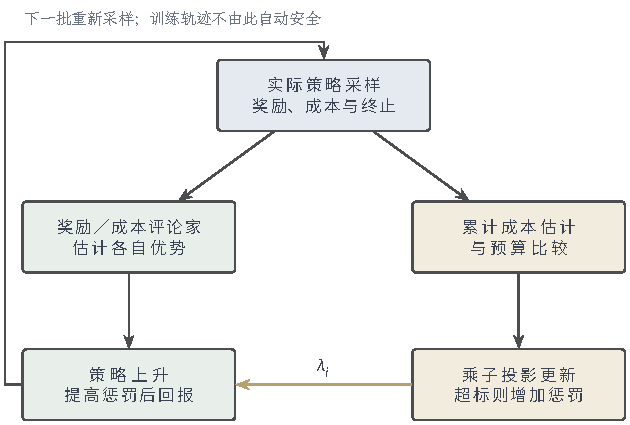
\includegraphics[width=106.659mm]{figures/10-reinforcement-learning/03-task-expansion-and-trustworthiness/tikz/rl-trustworthy-primal-dual.pdf}
  \caption{期望成本约束的两条反馈。奖励与成本优势共同推动策略更新，累计成本与预算的差推动乘子更新；这是一种求解循环，不是每次采样均满足约束的证书。}
  \label{fig:rl-trustworthy-primal-dual}
\end{figure}

\begin{theorem}[有限折扣CMDP的强对偶]
  \label{thm:rl-trustworthy-strong-duality}
  固定有限状态集、各状态非空有限动作集、转移核$T$和初态分布$\mu_0$，取$0\leq\gamma<1$。奖励$R(s,a)$、非负成本$c_i(s,a)$及有限预算$b_i$均固定且有界，$J$和$J_{c_i}$为从$\mu_0$启动的未归一化折扣期望。至少有一个满足全部预算的策略时，允许随机平稳策略的CMDP与占用度量线性规划等价，且
  \[
    \begin{aligned}
      \max_{\pi:\,J_{c_i}(\pi)\leq b_i}J(\pi)
        &=\min_{\bm{\lambda}\geq0}g(\bm{\lambda}),\\
      g(\bm{\lambda})
        &=\sum_i\lambda_i b_i+
          \max_\pi\left\{J(\pi)-\sum_i\lambda_iJ_{c_i}(\pi)\right\}.
    \end{aligned}
  \]
  原始最优解和有限维线性规划的对偶最优解存在。
\end{theorem}

证明以式~\eqref{eq:rl-trustworthy-cmdp-lp}~的占用量替代策略。可行占用集是非空、有界、闭多面体，线性目标有有限最优值，有限维线性规划强对偶因而给出相等的原始与对偶最优值。流守恒对应状态价值变量，成本不等式对应非负乘子；保留成本乘子并对占用流最大化，就得到定理中的$g$。这里使用的是原始问题非空且最优值有限的有限维线性规划强对偶，用于核对CMDP目标与乘子目标是否等价；相关基础可参考\BookChapterRef{chap:optimization}{卷1《数学准备：计算、分析与几何》“最优化”章}。

互补松弛还要求
$\lambda_i^\star(J_{c_i}(\pi^\star)-b_i)=0$：预算严格富余时乘子必须为0，预算恰好用尽时乘子却未必严格为正。强对偶依赖占用多面体的线性结构，不依赖任意神经网络参数集的凸性。参数化策略可能表示不了最优占用量，交替梯度也可能停在非全局解，因此上述定理不能直接当作神经网络训练的收敛保证。

乘子通过惩罚间接推动成本达标，\term{约束策略优化}（constrained policy optimization, CPO）则在旧策略附近直接限制一次更新的成本代理。代理沿用旧策略的状态分布，候选策略实际运行后却有新的状态分布，因此还需控制两者之差。令旧策略$\pi$与候选策略$\pi'$均为平稳Markov策略，对奖励或任一成本$f$定义
\[
  \begin{aligned}
    S_f(\pi',\pi)
      &=J_f(\pi)+\frac{1}{1-\gamma}
          \mathbb E_{s\sim d^\pi,a\sim\pi'}A_f^\pi(s,a),\\
    \epsilon_f
      &=\max_s\left|\mathbb E_{a\sim\pi'}A_f^\pi(s,a)\right|.
  \end{aligned}
\]
在共同MDP、共同初态和有界优势下，有
\begin{align}
  J(\pi')&\geq S_r(\pi',\pi)
      -\frac{2\gamma\epsilon_r}{(1-\gamma)^2}\overline D_{\mathrm{TV}},
      \nonumber\\
  J_{c_i}(\pi')&\leq S_{c_i}(\pi',\pi)
      +\frac{2\gamma\epsilon_{c_i}}{(1-\gamma)^2}\overline D_{\mathrm{TV}},
  \label{eq:rl-trustworthy-cpo-bound}\\
  \overline D_{\mathrm{TV}}
    &=\mathbb E_{s\sim d^\pi}
          \frac12\sum_a|\pi'(a\mid s)-\pi(a\mid s)|. \nonumber
\end{align}
式~\eqref{eq:rl-trustworthy-cpo-bound}~给回报下界和成本上界，方向不同，是因为收益需要不太低、成本需要不太高。其关键是占用变化界
$\|d^{\pi'}-d^\pi\|_1\leq
2\gamma\overline D_{\mathrm{TV}}/(1-\gamma)$。
性能差恒等式原本在$d^{\pi'}$下平均优势；将其换成$d^\pi$，用$\epsilon_f$乘上占用差，再除以$1-\gamma$，就得到上述误差项。若
$\mathbb E_{d^\pi}D_{\mathrm{KL}}(\pi'\|\pi)\leq\kappa$，Pinsker不等式和Jensen不等式进一步给出
$\overline D_{\mathrm{TV}}\leq\sqrt{\kappa/2}$。因此，精确求得
$S_{c_i}$加上误差余量不超过$b_i$，才直接推出下一策略成本达标。完整的界与CPO构造见原论文\scite{rl8-achiam2017-cpo}

实际CPO以样本优势、成本约束的一阶近似和KL的二阶近似求局部步，再用线搜索检查代理量；通常也没有精确估计$\epsilon_f$的全状态上界。只让线性化成本代理低于预算，至多得到仍带余项的成本界，不能据此省略余项而宣称严格可行。

Lagrangian PPO或SAC将乘子惩罚接入各自策略目标，仍继承对应采样和近似误差；SAC若包含熵奖励，所优化回报还发生了改变。奖励约束策略优化（reward constrained policy optimization, RCPO）采用便于学习的替代惩罚与多时间尺度更新，其收敛依赖替代惩罚和原约束的关系、步长及优化假设。任意换一个奖励，并不能由此推出原成本约束达标\scite{rl8-tessler2019-rcpo}

只有离线日志、不能继续试错时，乘子更新还面临另一项困难：候选策略改变状态访问分布，而原日志中的成本均值未必是候选策略的成本。COptiDICE（Offline Constrained Reinforcement Learning via Stationary Distribution Correction Estimation）沿用第~\ref{chap:rl-information}~章DICE的占用流校正，将固定策略评价扩展为带成本约束的占用优化。为看清其接口，仍取有限状态动作、时间不变MDP、$0\leq\gamma<1$、固定初态$\mu_0$及有界奖励和非负成本。日志训练样本$D$包含状态、动作、奖励、各项成本与下一状态，另需与目标启动条件相符的初态样本；令$d_D(s,a)$表示日志转移记录的状态动作抽样分布。它可以来自多种行为机制的混合，不要求已知某个单一行为策略$\beta(a\mid s)$。

把候选归一化占用写成$d(s,a)=d_D(s,a)w(s,a)$，其中$w\geq0$。与式~\eqref{eq:rl-information-dice}~评价固定目标策略不同，此处策略也待求解，因此先匹配状态流：对每个状态测试函数$v:S\to\mathbb R$，理想总体约束为
\begin{equation}
 \mathbb E_{(s,a)\sim d_D,\,s'\sim T(\cdot\mid s,a)}
   \left[w(s,a)\{v(s)-\gamma v(s')\}\right]
   =(1-\gamma)\mathbb E_{s_0\sim\mu_0}v(s_0).
 \label{eq:rl-trustworthy-coptidice-flow}
\end{equation}
全部$v$的约束对应式~\eqref{eq:rl-trustworthy-cmdp-lp}~的状态流守恒，使加权后的记录可解释为某个候选策略的折扣访问，而非任意提高高奖励样本的权重。方法在归一化奖励目标$\mathbb E_{d_D}[wR]$中减去$\eta\mathbb E_{d_D}f(w)$，其中$\eta>0$，$f$为满足$f(1)=0$的严格凸可微函数，以惩罚占用量过度偏离日志分布；成本约束配非负乘子，状态流配状态势函数，经对偶化用转移样本学习$w$。这一占用正则化会改变无正则CMDP的优化目标，不能将两者的最优回报直接等同。

只代入经验均值$\mathbb E_{d_D}[wc_i]$仍可能低估成本。COptiDICE进一步对成本作稳健的上侧估计：将初态样本与$(s,a,s')$转移记录组成的联合样本律作为扰动对象，限制其相对经验联合律的KL距离不超过$\epsilon_{\mathrm{rob}}\geq0$，并要求扰动后的初始分布、转移条件律及$\widetilde p(s,a)w(s,a)$仍满足同一占用流方程。随后求这些兼容分布下加权成本$\mathbb E_{\widetilde p}[wc_i]$的上确界，再将上侧估计经非负乘子接入策略优化。原论文的对偶成本目标因此含状态势函数的流残差修正，不能替换为只对状态动作边缘分布任取KL球的$\mathbb E[wc_i]$。$\eta$控制占用正则强度，$\epsilon_{\mathrm{rob}}$控制成本扰动范围，两者具有不同作用。由于这里$J_{c_i}$未归一化，归一化占用下的成本上侧估计应与$(1-\gamma)b_i$比较，不能直接与$b_i$比较\scite{rl8-lee2022coptidice}

获得满足相应流约束的占用比后，有限动作情形可按
\begin{equation}
 \pi_w(a\mid s)=
   \frac{d_D(s,a)w(s,a)}
        {\sum_{a'\in\mathsf A(s)}d_D(s,a')w(s,a')},
 \qquad \sum_{a'}d_D(s,a')w(s,a')>0
 \label{eq:rl-trustworthy-coptidice-policy}
\end{equation}
恢复候选策略。式~\eqref{eq:rl-trustworthy-coptidice-policy}~归一化的是日志状态动作质量乘占用比，不是要求先恢复原行为概率。例如只有一个自循环状态、两个动作$L,R$、初态就在该状态时，取$d_D=(3/4,1/4)$和$w=(1/3,3)$，得到候选占用$(1/4,3/4)$，其总质量为1，满足任意$0\leq\gamma<1$下的状态流；恢复的动作概率也为$(1/4,3/4)$。这是抽取步骤的手算示例，不是算法在某个基准上学得的结果。连续动作通常用$\mathbb E_{d_D}[w\log\pi_{\bm\theta}(a\mid s)]$作加权行为克隆，所提取策略还会增加函数逼近与拟合误差。

原总体推导以日志分布充分支持为条件；支持不全时只能在已覆盖的经验CMDP中求解。分母为0的状态可另选合法策略，但日志没有据此识别这些选择的回报或成本；$d_D(s,a)=0$处也不能靠有限权重创造正占用。还须存在受日志支持且满足所选成本稳健约束的候选方案，否则惩罚和乘子都不能创造缺失的可行策略。在精确求解相应稳健问题时，成本上界针对所声明的联合扰动集；真实运行律是否被该集合覆盖须另有依据，KL半径本身不构成普遍的有限样本安全保证。采样、流匹配函数类、比率优化与策略抽取误差仍需核查，最终固定策略的成本也仍须按第~\ref{sec:rl-trustworthy-inference}~节的评价协议取证。

理想占用规划的全局最优与强对偶、近似更新的误差控制、最终策略的原成本验证，至此已有各自依据。它们仍未约束每条训练轨迹：即使输出策略平均成本达标，先前探索也可能违反安全要求。要约束整个学习过程，还须明确其事件或硬安全标准。

% Outline: 8.4.2
\subsection{轨迹事件概率约束下的安全学习}
\label{sec:rl-trustworthy-chance}

第二类约束直接盯住“出事”这件事本身，而不是出事造成的平均成本。如果要求直接限制整次导航出事的可能性，平均碰撞成本就不是所需指标。例如规格要求发生任意碰撞的概率不超过1\%。设$E_t$为动作$t$导致碰撞的事件，定义
\[
  F_H=\bigcup_{t=0}^{H-1}E_t,\qquad
  \mathbb P_\pi(F_H)\leq\varepsilon.
\]
这就是\term{机会约束}（chance constraint）：允许违约发生，但指定事件的概率须不超过阈值。阈值来自任务要求，时域$H$决定哪些动作纳入事件。$\mathbf1\{F_H\}$不区分一次与多次碰撞，也不区分损坏1个与100个部件，因此相同失败概率仍可能对应不同事故成本。

首次碰撞之后再次碰撞，不应重复计入“至少发生一次”的概率。为保存这段历史，把失败标记加入状态：令$z_0=0$、$z_t\in\{0,1\}$，并递推
$z_{t+1}=z_t\lor\mathbf1\{E_t\}$。若原系统和碰撞判定在状态、动作与后继状态上是马尔可夫的，则$(s_t,z_t)$也是马尔可夫状态，且
$\mathbb P_\pi(F_H)=\mathbb E_\pi z_H$。
对于以状态集合$\mathcal B$表示的危险区域，也可令$z_0=\mathbf1\{s_0\in\mathcal B\}$，将初始失败纳入事件；两种起始约定不能混用。

固定时间相关策略$\pi_t$后，从终端标记向前求期望，即可得到概率价值$v_t(s,z)$：
\begin{align}
  v_H(s,z)&=z,\nonumber\\
  v_t(s,z)&=\sum_a\pi_t(a\mid s,z)
       \sum_{s'}T(s'\mid s,a)
         v_{t+1}\bigl(s',z\lor e(s,a,s')\bigr),
  \label{eq:rl-trustworthy-probability-value}
\end{align}
其中$e(s,a,s')$为本步事件指示量。按$t=H-1,\ldots,0$回传，最后对$\mu_0$平均$v_0(s,0)$，就得到整回合失败概率；若计入初始危险状态，则改为平均$v_0(s,z_0(s))$。这里求的是事件概率，不是折扣回报，因此不应额外乘奖励任务的折扣因子。在$z_0=0$的约定下，也可定义首次失败成本
$k_t=\mathbf1\{z_t=0,z_{t+1}=1\}$，则$\sum_tk_t=z_H$；普通碰撞次数之和一般不等于$z_H$。

把单步要求接成回合要求，只需同一概率空间上的事件关系。取正整数时域$H$和任意可测事件$E_0,\ldots,E_{H-1}$，并集界给出
\[
 \mathbb P(F_H)=\mathbb P\left(\bigcup_{t=0}^{H-1}E_t\right)
 \leq\sum_{t=0}^{H-1}\mathbb P(E_t).
\]
因此，非负预算若满足$\mathbb P(E_t)\leq\varepsilon_t$且$\sum_t\varepsilon_t\leq\varepsilon$，就支持整回合失败概率不超过$\varepsilon$。这个结论不要求各步事件独立，用途是把可检查的单步概率预算接到回合事件；相关概率工具可参考\BookChapterRef{chap:random-variables}{卷2《数学准备：概率、因果与决策》的“随机变量与概率基础”章}。

并集界将各步事件概率相加，一条轨迹上的多次碰撞可能被重复计入，所以界可能保守。若预算针对尚未失败时的下一步，则应改用存活条件。令
$S_t=\bigcap_{j<t}E_j^c$，在$\mathbb P(S_t)>0$时定义
$q_t=\mathbb P(E_t\mid S_t)$，则由条件概率乘法
\[
  \mathbb P(F_H)=1-\mathbb P(S_H)
       =1-\prod_{t=0}^{H-1}(1-q_t).
\]
取条件预算$\beta_t\in[0,1]$，则$q_t\leq\beta_t$推出
$\mathbb P(F_H)\leq1-\prod_t(1-\beta_t)\leq\sum_t\beta_t$。
乘积来自连续存活的条件概率链，不来自事件独立性。$q_t$已对所有存活历史求平均；要求每个存活历史下的条件概率都不超过$\beta_t$，是更强的充分条件。某时刻存活概率若为0，整回合失败概率已经是1，无须再定义后续条件概率。因此，无条件$\mathbb P(E_t)$、存活条件$q_t$和特定状态下的概率，不能共用同一预算解释。

教学计算中，若每步给定存活后的碰撞概率都是0.01，则$H=10$时整回合概率为
$1-0.99^{10}\approx0.0956$，$H=100$时为
$1-0.99^{100}\approx0.6340$。这两个数不需要额外假设各$E_t$独立，因为条件概率已被直接给定。若要求100步整回合不超过0.01，并且均匀分配条件预算，每步应满足
$\beta\leq1-0.99^{1/100}\approx0.00010050$。
图~\ref{fig:rl-trustworthy-events}~另将多个训练回合括在一起：最终策略单回合的$F_H$与训练期间任一回合出事的事件，具有不同样本空间和时域。

\begin{figure}[htbp]
  \centering
  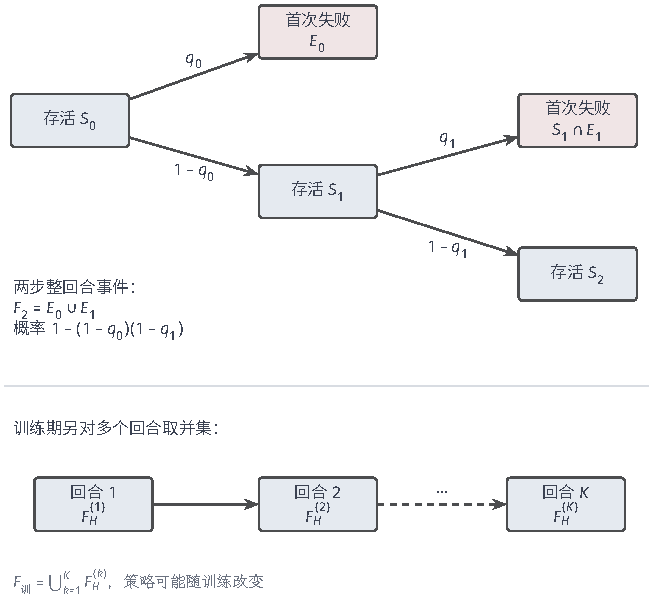
\includegraphics[width=110.652mm]{figures/10-reinforcement-learning/03-task-expansion-and-trustworthiness/tikz/rl-trustworthy-events.pdf}
  \caption{单步事件、整回合事件与整个学习过程事件。树在首次失败后合并成终止分支；下方回合可以使用不同策略，不能直接套用固定策略独立同分布的频率模型。}
  \label{fig:rl-trustworthy-events}
\end{figure}

事件定义明确后，学习方法取决于能否取得模型。直接采样时，每回合记录一次$z_H$，以均值估计概率，再用轨迹得分
$z_H\sum_t\nabla\log\pi(a_t\mid I_t)$估计概率梯度，并据此作拉格朗日约束更新。稀有事件使失败概率的相对误差更难控制，概率梯度也可能主要由极少数失败回合贡献；一批全为零的事件标记会使这份样本的梯度估计为0，但这只是没有观测到失败，不是安全证明。

模型已知时，可由式~\eqref{eq:rl-trustworthy-probability-value}~评价候选，或在时间和失败标记增广状态上优化期望终端成本，单次稠密评价代价为$O(H|S|^2|\mathsf A|)$。两种方法都需要完整事件标记；超时截断后未记录的事故，不能被当作没有发生。

如果不同后继状态需要不同风险余量，还可将剩余允许概率作为决策状态。到达尚未失败的$(t,s)$，剩余预算为$b\in[0,1]$，候选动作$a$的立即失败概率为$p_f(s,a)$，即对$e(s,a,s')=1$的后继转移概率求和。给未失败后继分配$b(s')\in[0,1]$，用全概率将立即失败和未来失败分开：
\begin{equation}
  p_f(s,a)+
    \sum_{s':\,e(s,a,s')=0}T(s'\mid s,a)b(s')\leq b.
  \label{eq:rl-trustworthy-risk-budget}
\end{equation}
\begin{samepage}
一个两分支计算可以说明后继预算的含义。设动作以0.1概率立即失败，以0.3和0.6概率分别到达两个安全后继$s_1,s_2$，这三项概率之和为1。给后继分配$b(s_1)=0.2$、$b(s_2)=0.05$，若两个后继的后续策略分别保证失败概率不超过这些预算，则整个后续失败概率的上界为
\[
  0.1+0.3\times0.2+0.6\times0.05=0.19.
\]
当前预算$b=0.2$时，这项分配通过当前一步的预算检验；整体可行还要求两个后继预算均可实现。到达$s_1$后，0.2是条件于已经到达该状态且此前未失败的后续概率上限；到达$s_2$后，相应上限为0.05。二者先经到达概率加权，才与立即失败概率一起接受当前预算检验，因此不能都用$0.2-0.1$作为同一个“剩余概率”。
\par
\end{samepage}

式\eqref{eq:rl-trustworthy-risk-budget}右侧的$b$限制的是条件于当前尚未失败状态的整个后续失败概率。选择满足该式且未来回报最高的动作与预算分配，到达$s'$后携带$b(s')$继续；最后一步后未来失败概率为0，向后归纳即可证明总概率不超过$b$。随机化动作时，还须对动作取平均并保留选定分支的预算。连续预算增加状态维度，网格化则带来规模和近似误差；随意从$b$减去一个“风险分数”没有对应的概率依据。

直接处理事件概率困难时，可以考虑CVaR的保守替代，但需要让损失编码与失败事件对应。令$X(\tau)>0$恰好表示失败，例如轨迹上最大的边界超出量。$X$可积时，有
\[
  \operatorname{CVaR}_{1-\varepsilon}(X)\leq0
  \quad\Longrightarrow\quad
  \operatorname{VaR}_{1-\varepsilon}(X)\leq0
  \quad\Longrightarrow\quad
  \mathbb P(X>0)\leq\varepsilon.
\]
第一个箭头依据尾部均值不小于分位点，第二个依据分位点定义；CVaR因而同时约束尾部严重程度，通常比原事件要求更强。反向不成立：以0.99概率取$X=-1$、以0.01概率取$X=100$，满足$\varepsilon=0.05$的机会约束，但最差5\%均值为
$(0.01\times100-0.04)/0.05=19.2>0$。若直接令$X=\mathbf1\{F_H\}$，则
$\operatorname{CVaR}_{1-\varepsilon}(X)=\min(1,p/\varepsilon)$；
把这一非负量限制为0，要求的是$p=0$，远强于原机会约束。采用替代目标前，须检查损失编码是否保留了所需事件含义，不能只匹配CVaR的名称和分位水平。

表~\ref{tab:rl-trustworthy-chance-methods}~将所需模型或记录与方法对应：完整回合支持直接采样，可信模型支持概率递推和预算分配，违约量的尾部分布支持CVaR替代。选择的既是求解手段，也可能是一个更保守的约束，因此须同时核对模型、采样条件和行为含义。

\begin{table}[htbp]
  \centering
  \begin{tabularx}{\linewidth}{@{}>{\raggedright\arraybackslash}p{21mm}XX@{}}
    \toprule
    方法 & 所需模型与记录 & 计算及主要边界 \\
    \midrule
    整回合采样 & 完整事件标记、固定时域与初态协议 & 每回合一个Bernoulli量；罕见事件样本少 \\
    概率价值递推 & 转移模型、时间、已失败标记 & 逐阶段备份；模型漏掉危险转移即失效 \\
    风险预算分配 & 上述模型、剩余预算及后继分配 & 增广预算空间；可行分配未必存在 \\
    CVaR替代 & 可积违约量及其尾部分布 & 同时限制尾部严重程度；通常更保守 \\
    \bottomrule
  \end{tabularx}
  \caption{机会约束的四种处理方式。它们分别解决估计、规划或保守替代问题，不能用相同数值阈值互相替换。}
  \label{tab:rl-trustworthy-chance-methods}
\end{table}

\begin{samepage}
若学习过程有$K$回合，记第$k$回合失败事件为$F_H^{(k)}$，训练期事件是
$F_{\text{训}}=\bigcup_{k=1}^KF_H^{(k)}$。即使每个训练回合都有概率上界$\varepsilon_k$，也只能直接得到
$\mathbb P(F_{\text{训}})\leq\sum_k\varepsilon_k$；自适应训练中可先对过去训练历史给条件上界，再用全期望与并集界。仅验证训练结束后的策略，完全没有约束先前探索使用的策略序列。
\par
\end{samepage}

% Outline: 8.4.3
\subsection{逐步与逐轨迹硬要求下的安全学习}
\label{sec:rl-trustworthy-hard-safety}

逐步与逐轨迹硬要求直接排除声明范围内的违规行为。这时候逐时刻检查“当前是否合法”是不够的。若要求任何时刻都不越界，检查当前机器人位置仍合法还不够：高速逼近边界且制动力不足时，即使此刻仍在界内，下一步也可能已经没有任何安全动作。硬安全需要的是往前看一步，找到那些“进去之后还能一直安全待下去”的状态。对已知离散系统
$\bm{x}_{t+1}=f(\bm{x}_t,\bm{u}_t,\bm{w}_t)$，用任务规格定义允许状态集$\mathcal X$，用执行器能力定义输入集$\mathcal U(\bm{x})$，用运行协议或模型误差界定义扰动集$\mathcal W(\bm{x},\bm{u})$。

\begin{definition}[控制不变集与可恢复集]
  \label{def:rl-trustworthy-invariance}
  对已知离散动力学$\bm{x}_{t+1}=f(\bm{x}_t,\bm{u}_t,\bm{w}_t)$，固定允许状态集$\mathcal X$、各状态可执行输入集$\mathcal U(\bm{x})$及输入确定后的允许扰动集$\mathcal W(\bm{x},\bm{u})$。
  集合$\mathcal K\subseteq\mathcal X$是鲁棒控制不变的，如果每个$\bm{x}\in\mathcal K$都有输入$\bm{u}\in\mathcal U(\bm{x})$，使所有
  $\bm{w}\in\mathcal W(\bm{x},\bm{u})$对应的后继状态仍在$\mathcal K$。
  一个从$\mathcal K$内选择这类输入的规则称为备份策略。
  给定备份不变集和非负整数步数$N$，可恢复集由那些存在非预见控制策略、能在所有允许扰动下始终留在$\mathcal X$并于至多$N$步进入$\mathcal K$的状态组成；非预见指本步输入只能使用已观察历史，不能使用尚未发生的扰动。
\end{definition}

定义中的量词顺序是“存在同一个输入，使所有允许扰动都安全”，不是针对每个扰动事后另选输入。允许状态集未必满足这一条件，可恢复集也随输入限幅、扰动范围和可用时间改变。若还要求整条轨迹成本不超过$B$，须保留剩余预算
$b_{t+1}=b_t-c_t$、$b_0=B$，并在增广状态$(\bm{x}_t,b_t)$上要求$b_t\geq0$及未来可行。折扣预算对应扣减$\gamma^tc_t$，或采用一致的相对时刻预算递推；不能用期望成本评论家替代每条轨迹的余额。

\begin{theorem}[安全集的一步封闭性保证]
  \label{thm:rl-trustworthy-invariance}
  考虑离散系统
  \[
    \bm{x}_{t+1}=f(\bm{x}_t,\bm{u}_t,\bm{w}_t).
  \]
  固定集合$\mathcal K\subseteq\mathcal X$、可执行输入集$\mathcal U(\bm{x})$和允许扰动集$\mathcal W(\bm{x},\bm{u})$。假定动力学$f$已知，实际状态可准确获得，初态$\bm{x}_0\in\mathcal K$，实际扰动始终在声明集合内。若每个$\bm{x}\in\mathcal K$的可行保护输入集合
  \[
    \begin{aligned}
      \mathcal U_{\mathcal K}(\bm{x})
        =\bigl\{\bm{u}\in\mathcal U(\bm{x}):\ &
          f(\bm{x},\bm{u},\bm{w})\in\mathcal K,\\
        &\text{对所有 }\bm{w}\in\mathcal W(\bm{x},\bm{u})\bigr\}
    \end{aligned}
  \]
  非空，且执行器在每步实际施加其中一个输入，则每条允许扰动轨迹都满足$\bm{x}_t\in\mathcal K$，$t\geq0$。
\end{theorem}
\begin{proof}
  固定任意满足扰动集合限制的轨迹。初始条件给出$\bm{x}_0\in\mathcal K$，这是归纳起点。
  假设在某个$t$有$\bm{x}_t\in\mathcal K$。集合非空保证能够选择
  $\bm{u}_t\in\mathcal U_{\mathcal K}(\bm{x}_t)$；按定义，对所有允许扰动，特别是实际发生的$\bm{w}_t$，
  \[
    \bm{x}_{t+1}=f(\bm{x}_t,\bm{u}_t,\bm{w}_t)\in\mathcal K.
  \]
  归纳步成立，故所有有限$t$都有$\bm{x}_t\in\mathcal K$。由于起初固定的轨迹任意，结论对每条允许扰动轨迹均成立。
\end{proof}

归纳证明把每步的全称保持条件传到整条轨迹，因此每项前提都影响结论。$\mathcal U_{\mathcal K}$若为空，就不存在满足要求的保护输入；状态判断若有误，所选动作可能不属于真实状态的可行集合；扰动越界或未建模延迟也会破坏一步封闭性。状态只能估计为集合$\widehat{\mathcal X}_t$时，须让同一个输入对全部可能真实状态和允许扰动有效，并另行保证真实状态确实在估计集合内。

定理~\ref{thm:rl-trustworthy-invariance}~也给出了执行检查：先有已验证不变集$\mathcal K$，再检查候选输入是否使全部允许后继仍在$\mathcal K$内。这样的数学条件及其成立依据称为\term{安全证书}（safety certificate），也就是可据以检验行为的证明条件。算法~\ref{alg:rl-trustworthy-filter}~使用这一不变集证书；屏障函数和预测过滤器则提供构造或检验保持条件的其他方式。距离最小的修正只用于尽量保留候选意图，并不产生安全性；只有保护输入集合非空且距离最小值取到时，算法才能要求最近点。若最小值不取到或求解器未在时限内返回经验证的可行点，只能改用当前仍满足同一保持条件的备份；集合为空或备份也未通过当前检查时，须报告保证失效。

\begin{algorithm}[带可行性检查的安全过滤]
  \label{alg:rl-trustworthy-filter}
  \begin{algorithmic}[1]
    \Require 候选策略、有效状态估计集合、动力学及误差集合、已验证不变集$\mathcal K$及其一步保持条件、可用备份
    \For{每个执行时刻$t$}
      \State 取得候选动作$\bm{u}^{\text{候}}_t$，更新状态估计集合
      \State 按定理~\ref{thm:rl-trustworthy-invariance}~构造保护输入集合：同一输入须使所有可能真实状态在所有允许扰动下的后继都留在$\mathcal K$
      \State 若候选动作在集合中，直接使用；否则，仅在最近点存在且求解器及时返回时使用距离最小的可行输入
      \State 若最近点不存在或优化超时，改用经过当前一步保持检查的备份；若集合为空或备份也不可行，报告保证失效并触发预设应急机制
      \State 执行实际动作，记录候选、实际动作、干预原因和后继状态，反馈给学习器
    \EndFor
  \end{algorithmic}
\end{algorithm}

过滤优化超时后，备份能否接管仍要在当前状态检查。应急停止只有满足相同模型和可行性条件时，才是证明中的安全输入；若已经没有安全制动距离，“优化失败就刹车”不能恢复已丢失的保证。图~\ref{fig:rl-trustworthy-filter}~因而将模型、状态估计和备份直接送入保护模块，并把实际动作反馈给学习器。

\begin{figure*}[t]
  \centering
  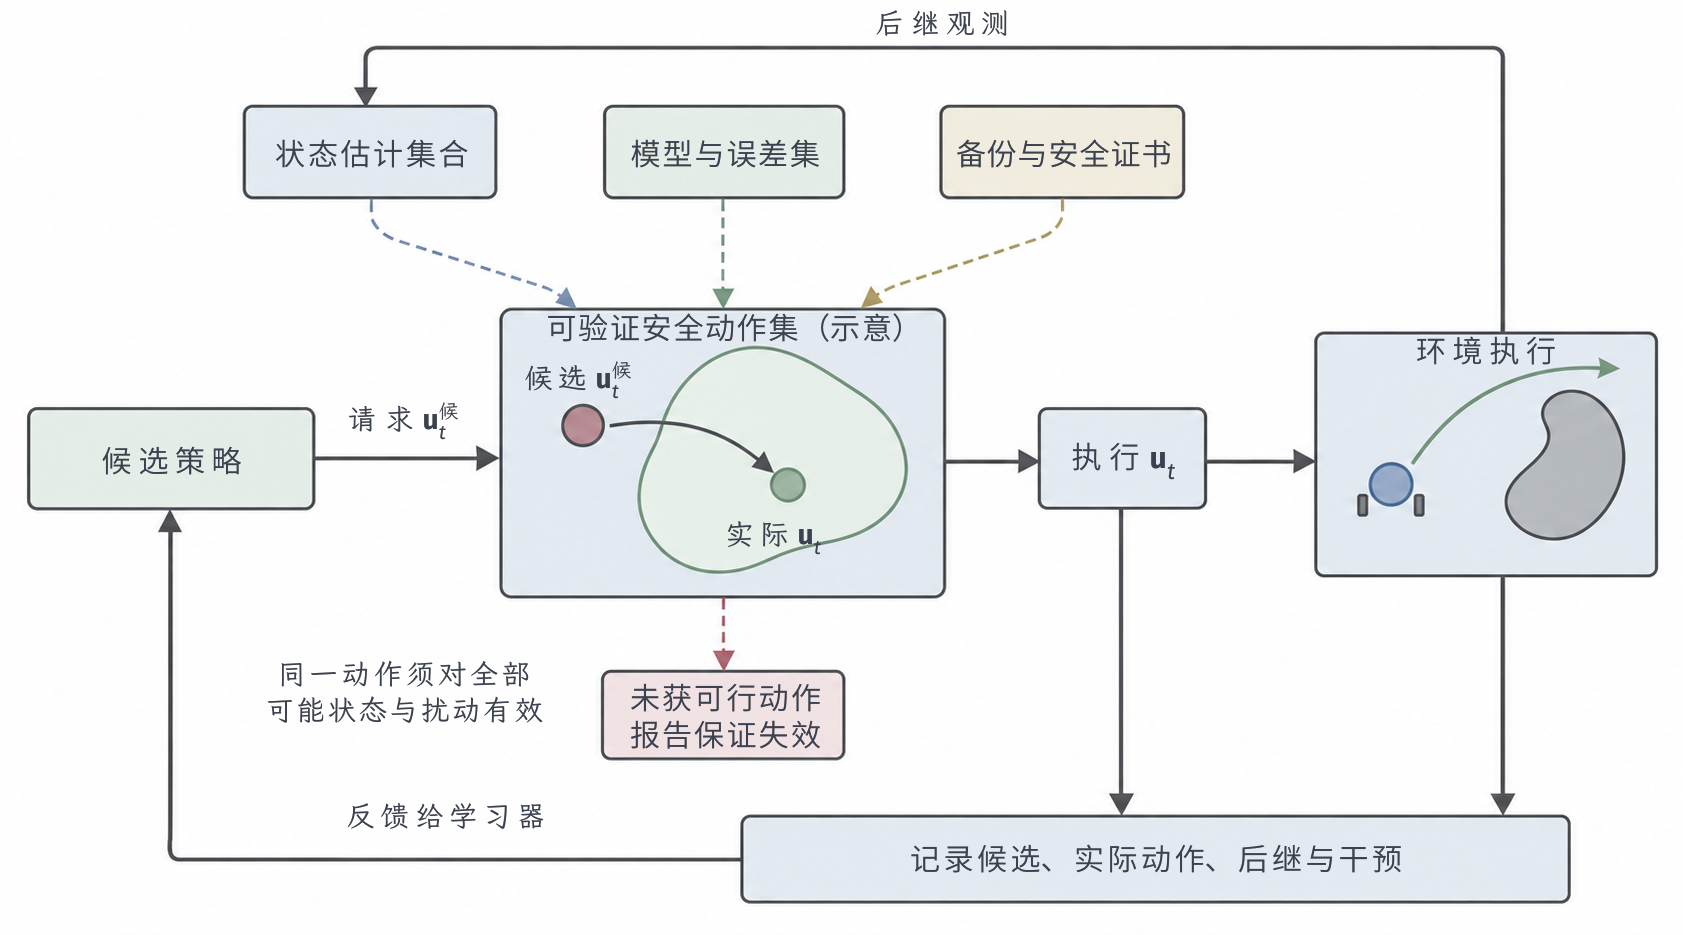
\includegraphics[width=157.400mm]{figures/10-reinforcement-learning/03-task-expansion-and-trustworthiness/generated/rl-trustworthy-filter/figure.png}
  \caption{保护器对控制动作的筛选与执行。实线连接候选动作、实际动作、环境和执行记录，虚线给出保护判断依赖的状态估计、模型与证书。动作区域仅为集合示意，不表示凸性、最近点存在或精确投影；未取得可验证动作时报告保证失效。右侧避障场景仅示意执行，评价仍须说明保护是否启用及保证针对哪个组合系统。}
  \label{fig:rl-trustworthy-filter}
\end{figure*}

离散动作下，可以屏蔽不满足一步保持条件的动作。若安全动作上的候选策略总质量为正，就将这些动作的原概率按该总质量归一化；若总质量为0，例如确定性候选只提出危险动作，则改用预先声明且经当前保持条件验证的备份分布。安全动作集为空，或备份分布不再受其支持时，屏蔽规则没有可执行的安全选择，必须报告保证失效。任务规格若含历史要求，屏蔽状态还可能包括表示规格进展的任务自动机或历史标记。普通\term{动作屏蔽}（action masking）只删除“向墙内移动”等即时非法动作，未必保留未来安全；按安全规格构造的屏蔽则在抽象模型上维护允许后继，其保证取决于抽象是否覆盖真实系统\scite{alshiekh2018shielding}

连续输入下，若可行集非空且最近点存在，可在其中找距离候选最近的动作，以尽量保留候选意图：
\[
  \min_{\bm{u}\in\mathcal U_{\mathcal K}(\bm{x})}
          \|\bm{u}-\bm{u}^{\text{候}}\|^2.
\]
教学系统$x_{t+1}=x_t+u_t+w_t$取$\mathcal K=[0,1]$、
$u_t\in[-0.2,0.2]$、$w_t\in[-0.05,0.05]$。鲁棒一步条件为
$0.05-x_t\leq u_t\leq0.95-x_t$。在$x_t=0.96$时，候选$u_t=0.1$会使最坏后继达到1.11；与输入限幅取交后，可行集为$[-0.2,-0.01]$，投影得到$u_t=-0.01$，后继范围为$[0.90,1.00]$。投影将朝边界的正动作改为负动作，是因为可行区间已计入最坏扰动；后继范围的显式计算才是保持安全的依据。

为了把“始终留在安全区”这一几何条件变成算法可以逐次检查的输入约束，\term{控制屏障函数}（control barrier function, CBF）用$h(\bm{x})\geq0$表示允许区域（状态安全当且仅当$h$非负），并限制输入使$h$不变为负。离散时间须检查
$h(f(\bm{x},\bm{u},\bm{w}))\geq0$对允许扰动成立，或者使用能够推出这一条件的更强不等式。连续时间控制仿射系统
$\dot{\bm{x}}=\bm{f}(\bm{x})+\bm{g}(\bm{x})\bm{u}$则常使用
\[
  \nabla h(\bm{x})^\top
       \bigl(\bm{f}(\bm{x})+\bm{g}(\bm{x})\bm{u}\bigr)
        \geq-\alpha_h(h(\bm{x})).
\]
其中$h$连续可微，$\alpha_h$是适当的扩展类$\mathcal K$函数，即连续、严格递增且$\alpha_h(0)=0$。不等式限制$h$下降的速度，使它在边界处不能继续朝负值方向穿越。在边界处$\nabla h\neq0$、声明时域内闭环解存在且唯一、输入约束下不等式始终可行、实际反馈满足不等式且初态在集合内等条件下，比较原理支持正向不变性，即闭环轨迹在声明时域内留在允许集合。它在此用于限制训练所得策略请求的动作；相关控制基础可参考\BookChapterRef{chap:policy-realization-and-control}{卷2《数学准备：概率、因果与决策》“策略的实现与轨迹控制”章}。

控制仿射性使输入以线性形式出现在约束中，常可和二次投影目标组成\term{二次规划}（quadratic program, QP）。输入饱和或多个约束冲突仍可能使QP不可行。连续时间不等式只约束所分析的连续闭环，采样间隔、执行延迟和模型误差还须通过余量或离散分析另行覆盖\scite{rl8-ames2017-barrier}

\term{预测安全过滤器}（predictive safety filter）把检查延伸到未来控制计划：预测时域内状态和输入都满足约束，末端进入已有备份能够维持的不变集，优化目标则可优先保留当前候选动作\scite{rl8-wabersich2021-filter}
鲁棒版本须使用反馈计划或误差管束；管束保存的是各步所有允许状态，而非一条标称避障轨迹。若执行一步后真实状态仍在旧的可行管束内，下一时刻就可向前平移旧计划，并在末端接上备份控制。这给出递归可行性的依据，即本次可行能为下一次留下可行方案。

误差集合突然扩大、终端集失效、状态估计离开管束或求解未按时完成，都可能破坏这一依据。预测步数、状态维度和非线性误差传播还决定在线代价，因此采用“MPC过滤”并不免除模型覆盖、可行性和求解时限的检查。

过滤维持当前可行性，恢复控制则把系统带回已验证区域，并须在返回过程中保持约束。停止学习任务、返回安全种子可以是整体方案的一部分。近期安全复位研究联合建模到达复位区域与避开危险；无人干预学习因此还要检查回合之间的重置，而不只检查单回合动作。这扩大了保证时域，也增加了复位路径、时间和控制能力的要求，不能假定复位天然安全或没有代价\scite{rl8-begzadic2025-reset}

上述过滤依赖动力学，模型未知时通常要从已知安全种子区域或备份控制开始，用保护器实际执行后取得的状态、实际动作及后继状态记录缩小模型误差集，再扩展可验证区域。高斯过程（Gaussian process, GP）可以预测均值与不确定区间；但证书需要真实动力学在声明状态输入范围及所有取证时刻上，以至少$1-\delta$的概率同时被模型集合覆盖。联合覆盖通常依赖函数正则性、噪声假设、置信参数及对自适应采样的控制。稳定性证书与GP误差界相结合的安全学习依赖这些条件，单有预测方差还不能支撑安全声明\scite{rl8-berkenkamp2017-safe}

记联合模型覆盖事件为$C_{\mathrm{cov}}$，结论可分两步表述：“在$C_{\mathrm{cov}}$上，过滤器按不变性条件保持安全；取证程序满足$\mathbb P(C_{\mathrm{cov}})\geq1-\delta$。”前一步是条件于模型覆盖的逻辑保证，后一步才是统计覆盖。单个点的95\%预测区间不能替代整条闭环轨迹的联合事件。扰动若有无界支持，也不能无条件假定所有时刻均在有界集合内；有限时域高概率覆盖与无限时域逐轨迹保证须分别论证。

多机器人共享狭窄通道时，两个机器人若都假定“对方会等待”，各自可能有可行计划，联合执行却会相撞。团队保证因而还须核对联合输入约束、通信延迟和参与者的建模承诺。去中心化过滤只有在局部假设相容、联合可行域非空且执行时可读取的观测、状态与消息符合证明条件时，才可能支持团队安全；个体QP各有一个解不够。参与者响应模型仍由第~\ref{chap:rl-multi-agent}~章提供。

% Outline: 8.5
\section{可靠性评价与保证}
\label{sec:rl-trustworthy-evidence}

前面几节解决的是“怎样求出一个试图满足要求的策略”，但求解器在训练中优化了某个代理目标，不等于交付对象真的满足原要求；受保护系统长期无事故，也可能只是保护器在起作用，无法说明移除保护后的表现。所以还需要一个独立于训练的取证环节：预先固定取证协议，再依据评价样本或模型证明，估计各项指标落在什么范围、保证覆盖到哪里。图~\ref{fig:rl-trustworthy-validation}~显示这一依赖：运行条件改变时，旧成功次数是否仍可使用，须先重新核对协议。

\begin{figure*}[t]
  \centering
  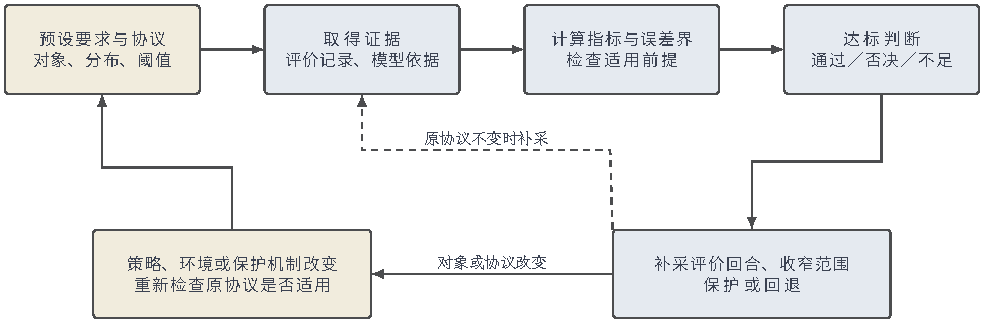
\includegraphics[width=166.617mm]{figures/10-reinforcement-learning/03-task-expansion-and-trustworthiness/tikz/rl-trustworthy-validation.pdf}
  \caption{运行记录、性能估计与可靠性判断之间的依赖。判断可以触发补充取证、收窄范围、保护或回退；原协议不变时，虚线返回允许补采记录。评价对象、保护配置或协议改变时，先重新核对协议，再取证和估计。流程本身不替代统计覆盖或模型证明。}
  \label{fig:rl-trustworthy-validation}
\end{figure*}

% Outline: 8.5.1
\subsection{确定验证协议并取得证据}
\label{sec:rl-trustworthy-protocol}

取证的第一步不是算统计量，而是把“这次运行到底在检验什么”固定下来。导航验证可以改变初始位置、训练种子或摩擦条件，但三种变化回答不同问题。固定策略从不同位置启动，评价其运行分布；换种子重新训练，评价学习规则产生的训练模型的变化；同一系统换摩擦条件，检查声明运行范围。未经区分就汇总成功率，会把策略、初态与环境三方面的影响混在一起，无法归因。

协议首先按保证对象冻结不同内容。评价固定策略或策略与保护层的组合时，冻结交付策略和保护器版本；评价固定学习规则的重复训练时，冻结训练流程、训练记录的生成与采样机制、训练样本预算、种子分布以及输出策略的验收规则，单次训练产生的输出策略本身是随机对象，不能事先冻结。随后再确定统计单位、初态与环境抽样分布、时域和终止规则、允许扰动与参与者、失败判定、回报与成本阈值及置信要求。这些约定决定怎样把一次运行或一次完整训练转成证据。碰撞若定义为“机身越过边界”，仅记录报警就不足以判定事件。恢复时间也须约定起点和恢复集合；观察结束仍未恢复，意味着真实恢复时间尚不完整，应按删失或超时规则处理，不能删去这些回合后计算平均值。

表~\ref{tab:rl-trustworthy-evidence-sources}~对应证据来源与可支持结论。模型证明覆盖显式模型的全部允许情况，运行试验则有助于发现实际系统中的模型遗漏。两者可以互补，但模型前提和试验抽样范围都须保留在结论中。

\begin{table*}[t]
  \centering
  \begin{tabularx}{\linewidth}{@{}>{\raggedright\arraybackslash}p{23mm}XXX@{}}
    \toprule
    证据来源 & 统计单位与可控条件 & 可支持结论 & 关键缺口 \\
    \midrule
    重复训练 & 一次完整训练；算法、预算、种子分布固定 & 输出策略指标分布、训练失败概率 & 不能只挑最好种子报告 \\
    固定策略重复运行 & 一回合；策略和运行协议冻结 & 协议分布下的回报、成本和事件概率 & 回合独立性、有效样本量 \\
    压力测试 & 指定极端场景或攻击；权限固定 & 已测条件下的失效及响应 & 不直接给常态运行失败频率 \\
    已有日志 & 日志中的回合；行为机制可追溯 & 覆盖与校正条件下的离线评价 & 漏报事件、选择性记录、支持不足 \\
    形式化模型分析 & 模型中的状态、轨迹或扰动集合 & 前提成立时的全称性质 & 真实系统是否满足抽象与误差前提 \\
    \bottomrule
  \end{tabularx}
  \caption{取证方式与保证对象的对应关系。重复训练的一条学习曲线不是一次固定策略运行，主动挑选的极端情况也不是从日常运行分布随机抽到的回合。}
  \label{tab:rl-trustworthy-evidence-sources}
\end{table*}

要避免选择偏差，最终检验使用的任务与运行记录也须与开发使用的任务及训练记录区分。任务、攻击和训练种子一旦用于更新策略，就不再是未使用的测试证据；验证集若用于反复挑选策略，也已参与选择。可以分开开发、策略选择和最终验收，或事先使用对整个候选类同时有效的界。只留出随机种子仍不够：困难地形若被反复用于调节保护阈值，这些地形上的运行反馈已经参与方案调整。对预先冻结的候选，独立评价样本支持相应的固定候选风险界；从同一批样本中选择候选时，须让界同时覆盖预定候选类，或在选择后另取独立评价样本。相关原则可参考\BookChapterRef{chap:trust-reliability}{卷3《基础、理论与可信性》“可靠性”章}。

为还原执行机制，每回合须保留初始条件、请求动作、实际动作、奖励、损失、成本、事件标记、接管时刻和恢复时间。失败后的运行记录有助于诊断后果和恢复，不应因回合“已经失败”而从日志消失。干预率还须固定分母：被替换动作占总动作的比例，和至少接管过一次的回合比例，衡量的是不同性质。

稀有事件的难点是有效危险样本少，复制成功轨迹不会增加独立的运行记录。重要性采样可以提高危险场景出现频率，但须知道目标运行分布相对采样分布的密度比、覆盖目标支持，并对完整事件统计加权。主动压力测试若没有这一密度比，只提供所测场景的证据。相关回合、长轨迹的重叠窗口或共享未重置环境状态的连续试验，也不能直接计作独立样本。

% Outline: 8.5.2
\subsection{由证据估计指标与保证范围}
\label{sec:rl-trustworthy-inference}

协议固定、评价记录收集完成后，下一步才是从有限样本估计指标，并说明这些估计可能偏出真实值多远。策略和协议冻结后，第$j$条完整轨迹给出$G_j,L_j,C_{i,j}$与失败标记$Y_j=\mathbf1\{F_H^{(j)}\}$。回报和成本可取样本均值，失败概率可取$\widehat p=n^{-1}\sum_jY_j$；尾部损失则需经验分位数或式~\eqref{eq:rl-trustworthy-cvar}~的样本目标。各统计量使用的轨迹函数与损失样本不同：CVaR主要依赖少量尾部质量，不能直接沿用回报均值的标准误；恢复时间则须纳入观察结束仍未恢复的回合。

由评价样本计算的点估计只是一个数。置信界控制推断程序的覆盖错误，模型误差界控制近似模型与真实系统的偏差，形式化性质则给出前提下的逻辑结论。三者不能互相替代。单回合内状态可以高度相关，只要回合独立，整回合失败标记仍可作Bernoulli分析；把每步当成独立回合，却会同时改变事件和有效样本量。

对预先冻结的策略、运行分布和失败事件，固定正整数样本量$n$。若完整回合的失败标记独立同分布为$\operatorname{Bernoulli}(p)$，取$0<\delta<1$，观察到零次失败时，精确二项单侧置信上界为
\[
 U_0(n,\delta)=1-\delta^{1/n}.
\]
这里用它判断完整运行记录能否支持部署失败概率阈值；它不证明$p=0$，也不覆盖根据已见评价记录选择样本量或策略的未经校正程序。相关保证与证据原则可参考\BookChapterRef{chap:trust-foundations}{卷3《基础、理论与可信性》“可信机器学习基础”章}。

覆盖性质可以按一个完整推断程序理解：零失败时返回$U_0$，出现失败时返回1。真实$p\leq U_0$时它从不漏盖，$p>U_0$时漏盖只能发生在零失败批次，概率为$(1-p)^n<\delta$，所以程序覆盖率至少为$1-\delta$。这是重复抽样程序的保证，不是关于固定$p$的后验概率。

这个上界可以检查零失败记录是否足以支持部署阈值。取$\delta=0.05$，100次零失败的95\%单侧上界约为0.029513，即2.95\%，还不能支持1\%阈值。令$1-\delta^{1/n}\leq\varepsilon$并解出样本量，得到事先应选择
\[
  n\geq
  \left\lceil\frac{\log\delta}{\log(1-\varepsilon)}\right\rceil.
\]
因此，1\%阈值至少需要299次，0.1\%阈值至少需要2995次。表~\ref{tab:rl-trustworthy-zero-failure}~列出公式计算值，不是机器人实验结果。成功回合较多与能够排除指定稀有失败水平，是不同结论。

\begin{table}[htbp]
  \centering
  \begin{tabular}{@{}rrl@{}}
    \toprule
    固定样本量$n$ & 95\%失败概率上界 & 与阈值比较 \\
    \midrule
    100  & 0.02951305 & 尚不能支持$p\leq0.01$ \\
    299  & 0.00996915 & 支持$p\leq0.01$ \\
    1000 & 0.00299125 & 尚不能支持$p\leq0.001$ \\
    2995 & 0.00099974 & 支持$p\leq0.001$ \\
    \bottomrule
  \end{tabular}
  \caption{零失败的解析教学上界。每行分别代表预先固定样本量的独立验证，不代表持续查看同一次试验并在达标时停止的程序。}
  \label{tab:rl-trustworthy-zero-failure}
\end{table}

如果不允许运行候选策略而只有日志，先要判断日志能否识别其风险。按第~\ref{chap:rl-information}~章的轨迹重要性采样，固定共同环境、初态与完整记录字段，设已知行为机制$\beta$覆盖目标$\pi$。动作有限或可数时，可用沿途动作点概率比
$W_j^\pi=\prod_{t=0}^{H-1}\pi(a_{j,t}\mid I_{j,t})/
\beta(a_{j,t}\mid I_{j,t})$。
连续动作则要求目标条件动作核相对行为条件动作核绝对连续，将每个因子改为前者相对后者的Radon--Nikodym导数，在已记录动作处求值；若使用密度比，还须声明共同支配测度。对能由完整记录计算、且在目标下可积的$G,C_i$，就有
$\mathbb E_\beta[W^\pi G]=J_H(\pi)$及
$\mathbb E_\beta[W^\pi C_i]=J_{c_i,H}(\pi)$。
权重将行为分布下的期望换成目标分布下的期望，失败事件同样可用$W^\pi Y$估计。动作覆盖还不等于日志完整：碰撞后结果若被删去，权重不能恢复缺失记录。隐藏混杂、执行通道变化或目标动作无支持，都可能使安全指标无法由日志识别。

要同时检验性能改进和成本达标，可以分别构造回报差下界与成本上界。设固定候选$\pi$和固定基线$\pi_b$共用$n$条独立同分布行为回合，两者轨迹分布都相对行为分布绝对连续，即目标可能轨迹在行为分布下也有支持；只覆盖候选不足以评价它与基线之差。定义
$Z_j=(W_j^\pi-W_j^{\pi_b})G_j$与
$X_{i,j}=W_j^\pi C_{i,j}$。若已知
$Z_j\in[z_-,z_+]$、$X_{i,j}\in[0,x_{i,+}]$几乎处处成立，则Hoeffding不等式给出
\begin{align}
  J_H(\pi)-J_H(\pi_b)
     &\geq \overline Z
        -(z_+-z_-)\sqrt{\frac{\log(1/\delta_r)}{2n}}
        =:\mathrm{LCB}_{\Delta J}, \nonumber\\
  J_{c_i,H}(\pi)
     &\leq \overline X_i
        +x_{i,+}\sqrt{\frac{\log(1/\delta_i)}{2n}}
        =:\mathrm{UCB}_{c_i}.
  \label{eq:rl-trustworthy-offline-joint}
\end{align}
换测度恒等式给出$\mathbb E Z$为回报差、$\mathbb E X_i$为候选成本，再对有界独立样本分别施加单侧浓缩不等式，即得到式~\eqref{eq:rl-trustworthy-offline-joint}~。此处独立单位是一回合完整可见记录，已知权重和累计量的界使所估变量有界，因而满足所用单侧集中界的抽样条件。回报差从均值减去余量，成本从均值加上余量，分别保留所需的不利方向。用并集界，所有声明同时成立的概率至少为
$1-\delta_r-\sum_i\delta_i$，无须各估计量相互独立。检验
$\mathrm{LCB}_{\Delta J}\geq-\epsilon_{\text{改进}}$与
$\mathrm{UCB}_{c_i}\leq b_i$，才分别支持“不比基线差太多”和“成本达标”。折扣无限时域评价还要补上截断余项。

这套界的强假设是权重和结果有已知界；长时域的乘积权重可能极大，置信区间也就可能宽到无法判断。截断权重能降低方差，却引入须另行控制的偏差；模型辅助估计则引入模型前提。

基线自举的安全策略改进（safe policy improvement with baseline bootstrapping, SPIBB）将支持不足区域的行为限制在基线附近，研究相应行为日志与模型假设下的期望回报改进。这里的“safe”针对相对基线的性能，不直接针对成本或碰撞概率：基线可能本就不安全，候选也可能以较高风险换取较高回报。行为安全仍需单独的成本或事件上界\scite{rl4-laroche2019-spibb}

候选$\pi$若由同一批评价样本选出，固定策略的式~\eqref{eq:rl-trustworthy-offline-joint}~就不能原样使用。可以对预先确定的有限候选集分配总错误预算，采用对策略类一致有效的界，或冻结最终策略后使用独立留出评价样本。日志中的动作若被保护器替换，权重分母须描述实际行为机制；目标也是受保护系统时，分子也须描述组合机制。只有概率比对应交付对象，估计才是在回答其性能和安全问题。

表~\ref{tab:rl-trustworthy-indicators}~汇总各指标的覆盖条件。回报、尾部、事件和恢复过程可以来自同一份日志，误差控制却须分别建立；不变性还需核对真实闭环是否满足证书前提，不能由日志均值代替。

\begin{table*}[t]
  \centering
  \begin{tabularx}{\linewidth}{@{}>{\raggedright\arraybackslash}p{19mm}XXXX@{}}
    \toprule
    指标或性质 & 估计／验证方法 & 覆盖条件 & 主要误差来源 & 保证对象 \\
    \midrule
    平均回报、成本 & 回合均值、离线校正与单侧界 & 固定策略和协议；独立或已处理相关性 & 抽样、截断、权重与模型偏差 & 指定策略的期望值 \\
    尾部损失、动态风险 & 累计损失的分位及CVaR估计；嵌套目标另需逐阶段条件估计 & 损失与尾部样本假设；动态目标还需条件分布覆盖 & 稀有样本、阈值估计、选择及递推误差 & 事先声明的累计或动态风险 \\
    失败概率 & 完整事件频率、二项或加权界 & 事件、时域、运行分布明确 & 漏报、相关回合、分布改变 & 固定执行系统的回合事件 \\
    恢复时间 & 完整或删失的恢复时间记录分析 & 恢复集合、起止和删失规则固定 & 超时删除、选择性接管 & 指定恢复机制 \\
    不变性 & 模型、误差集、可行性证明 & 真实闭环满足全部模型前提 & 状态估计、未建模执行与越界扰动 & 证书覆盖的保护系统 \\
    \bottomrule
  \end{tabularx}
  \caption{不同指标需要不同的误差控制。一个回报评论家准确，并不意味着碰撞概率或尾部损失已被准确估计。}
  \label{tab:rl-trustworthy-indicators}
\end{table*}

模型校准也需要明确分布：价值、后果分布和世界模型应在哪个策略诱导分布下接受检查？在训练轨迹经常访问的环境状态上预测准确，未必覆盖新策略频繁访问的边界状态；多个模型一致，也可能共同漏掉危险机制，所以集成分歧不自动构成置信界。形式化结论还须逐项核对真实动力学、状态估计、保护动作与执行器，不能只检查名义控制算法。

% Outline: 8.5.3
\subsection{依据要求作出判断并持续复核}
\label{sec:rl-trustworthy-decision}

有了带误差范围的指标界，还要按正确的方向与阈值比较，并如实区分“达标、不达标、证据不足”三种结论，而不是非黑即白地只看点估计。指标界得到后，应在不利方向与阈值比较。失败概率要求$p\leq\varepsilon$时，$U_p\leq\varepsilon$支持达标，$L_p>\varepsilon$支持不达标；区间跨阈值则现有样本尚不足以判断是否达标。回报要求$J\geq j_{\min}$时方向相反，$L_J\geq j_{\min}$支持达标，$U_J<j_{\min}$支持不达标。多项要求还须预先控制联合置信错误率，各项分别有95\%区间并不意味着整体仍有95\%覆盖。

图~\ref{fig:rl-trustworthy-intervals}~上半部分中，两组零失败评价记录的点估计都为0，但100次试验的上界仍高于1\%，299次的上界才低于1\%。下半部分只用示意区间展示回报应检查下界，没有对应实验。样本尚不足以判断是否达标时，可按新的预设方案补充证据，或收窄部署范围到已有覆盖的条件。此时尚不能确认达标，也没有证实不达标；直接批准原范围部署同样缺少依据。

\begin{figure*}[t]
  \centering
  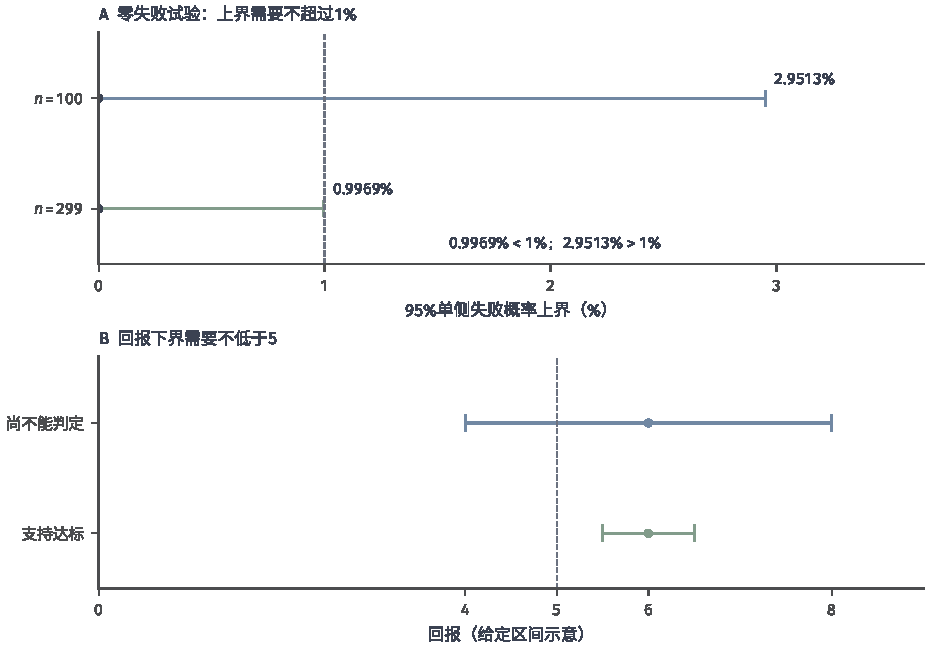
\includegraphics[width=157.400mm]{figures/10-reinforcement-learning/03-task-expansion-and-trustworthiness/matplotlib/rl-trustworthy-intervals.pdf}
  \caption{置信界与阈值的方向。上图按$n$次零失败的解析公式计算95\%单侧上界；下图仅以给定区间示意回报判断，不代表某个统计估计器或实验。点标估计，线段标可支持的指标范围。}
  \label{fig:rl-trustworthy-intervals}
\end{figure*}

达标判断还须绑定策略和协议版本。摩擦范围改变会影响轨迹分布，策略更新会影响状态动作占用，保护器升级会改变执行行为，参与者增加会改变闭环假设。旧运行记录未必全部失效，但须逐项说明哪些条件仍匹配、哪些运行记录需要重加权或补充、哪些模型性质须重新证明。交付对象或运行范围不再匹配时，旧安全声明不能直接沿用。

持续运行时，监测应检查保证前提：误差是否越出集合、备份是否仍可行、事件记录是否完整、干预比例是否明显改变。变化可触发保护、回退、收窄范围或补充取证，监测基础设施由系统卷讨论。统计判断也要覆盖查看方式：反复查看固定样本区间直到首次达标，并不自动保留原错误率。可预先为多次检验分配错误预算，或在相应评价记录的抽样条件下使用\term{置信序列}（confidence sequence），即对整个查看时间序列同时有效的界\scite{rl8-howard2021-sequences}

% Outline: 8.6
\section{多种要求的组合与取舍}
\label{sec:rl-trustworthy-combination}

三类要求至此分别讲完。为避免在不同任务上比较而让“任务本身的差异”掩盖“准则的差异”，现在把三类要求用于同一个导航选择。将基准网格抽象成单步路线选项任务：初态固定为起点，动作一次选择整段路线，结果给出到达终点总用时$T$、碰撞标记$I$和成本$C=10I$。这是独立教学模型，不使用基准网格的0.8滑移核；取$H=1$、不折扣、回报$G=-T$和损失$L=T$。路线内部的执行与恢复汇总为一次结果，时间以教学单位计。

候选集合先限定为四条确定路线A、B、C、D，所有比较固定同一初态和这组候选。干燥环境下，A以0.95概率用时5、以0.05概率用时25，B、C、D分别固定用时7、8、9。湿滑环境只将A、B用时各增加10，C、D不变。允许环境集合在本例中由这两个教学情形枚举给定，不是从观测记录估计的置信集。

两种环境中的碰撞概率依次为0.02、0.005、0.003、0。为分离时间与安全成本的影响，规定$I$和$T$独立，碰撞也不另外终止路线选项。这些假设共同确定联合分布，仅服务于控制变量比较，不是关于真实机器人碰撞与恢复的经验规律。

表~\ref{tab:rl-trustworthy-comparison}~据该联合分布精确计算。例如A平均用时为
$0.95\times5+0.05\times25=6$，0.95分位水平的CVaR为25，期望成本为$10\times0.02=0.2$，其余行用同样公式计算。回报越大越好，用时尾部、碰撞概率和成本越小越好。全部路线都关闭外部保护，干预为0；这只是固定执行机制，不是安全达标的证据。

\begin{table*}[t]
  \centering
  \begin{tabularx}{\linewidth}{@{}>{\raggedright\arraybackslash}p{14mm}XXXXXXX@{}}
    \toprule
    路线 & 标称平均回报 & 标称尾部损失 & 湿滑平均回报 & 碰撞概率 & 期望成本 & 干预比例 & 证据强度 \\
    \midrule
    A：捷径 & $-6$ & $25$ & $-16$ & $0.02$ & $0.20$ & $0$ & 教学模型精确值 \\
    B：定时 & $-7$ & $7$ & $-17$ & $0.005$ & $0.05$ & $0$ & 教学模型精确值 \\
    C：抗滑 & $-8$ & $8$ & $-8$ & $0.003$ & $0.03$ & $0$ & 教学模型精确值 \\
    D：保守 & $-9$ & $9$ & $-9$ & $0$ & $0$ & $0$ & 教学模型精确值 \\
    \bottomrule
  \end{tabularx}
  \caption{同一候选集合的解析教学比较。尾部损失为$\operatorname{CVaR}_{0.95}(T)$；碰撞概率和成本在两环境下按假设相同。D的零概率仅属于该指定模型，所有行均无真实部署统计证据。}
  \label{tab:rl-trustworthy-comparison}
\end{table*}

只最大化标称平均回报，会选A，却留下25的最差5\%平均用时。改为最小化标称尾部损失，选B，但其平均回报从干燥时的$-7$降到湿滑时的$-17$，回报减少10，也就是平均用时增加10。若最大化干燥与湿滑中的最坏平均回报，则选C；若仍优化标称均值，只增加期望成本预算$b=0.01$，四个确定候选中只有D可行。同一策略跨环境的下降幅度，还须与变化后的绝对值一起看：C、D的平均回报都没有下降，但变化后分别为$-8$与$-9$；若要求平均用时不超过8.5，C满足而D不满足。反过来，只看湿滑回报也无法区分原来就慢与湿滑额外造成的延误。这里的比较仍固定初态、候选和用时单位，每次求解只改一类要求，并非四个依次执行的算法阶段。

允许策略类若扩大到出发前随机选路线，结论还会变化。以0.2概率选B、0.8概率选D，期望成本为$0.2\times0.05=0.01$，平均用时为$0.2\times7+0.8\times9=8.6$，优于确定选D的9。因此D的上述最优性只针对四个确定候选，与示例~\ref{ex:rl-trustworthy-randomization}~相符。一次运行仍会完整选择B或D，不会走一条“平均路线”，B回合的碰撞可能也仍存在。

上面每次只施加一类要求。当它们同时出现时，不能简单地先按一个准则选策略、再指望它碰巧满足其余要求，而要把“在满足其余要求的策略中优化主目标”写成一个带约束的优化问题。这些要求若同时存在，须先由物理范围、枚举场景或观测记录给出的覆盖界确定模型族$\mathcal M$，再确定允许策略类$\Pi$。可以在保证最坏回报不太低、最坏成本不太高的前提下，最小化最坏风险：
\begin{align}
  \min_{\pi\in\Pi}\quad&
      \sup_{M\in\mathcal M}\mathcal R_M(L^\pi), \nonumber\\
  \text{满足}\quad&
      \inf_{M\in\mathcal M}J_M(\pi)\geq j_{\min}, \nonumber\\
  &\sup_{M\in\mathcal M}J_{c_i,M}(\pi)\leq b_i
       \quad (i=1,\ldots,m_c).
  \label{eq:rl-trustworthy-combined-problem}
\end{align}
这里$\mathcal R_M$须事先选为静态或动态风险，$\Pi$须说明历史依赖和随机化范围。风险与成本越大越差，故对模型取上确界；回报越小越差，故取下确界。这使每项要求分别覆盖全部允许模型。在路线例中，$\mathcal M$可以就是干燥与湿滑两情形；没有场景概率时，不能对二者作概率平均，即使给出概率，平均达标仍可能由干燥时的收益抵消湿滑时的违反，不能代替逐模型约束。只对回报作鲁棒优化，不会自动使成本鲁棒；鲁棒成本达标也不保证任务收益足够。

图~\ref{fig:rl-trustworthy-intersection}~将各项阈值对应的允许策略画成集合，最终可行域是这些集合与$\Pi$的交集。固定目标和策略类后，增加约束只能保持或缩小可行域，不会使最优值自动改善。在四个确定路线中，同时要求标称CVaR不超过8、最坏平均用时不超过9、期望成本不超过0.01，就没有可行选项：C满足前两项而成本超标，D满足后两项而尾部用时为9。此时须扩大策略类、改变环境或协商阈值；求解器返回的最少违反方案仍未满足原要求。

\begin{figure}[htbp]
  \centering
  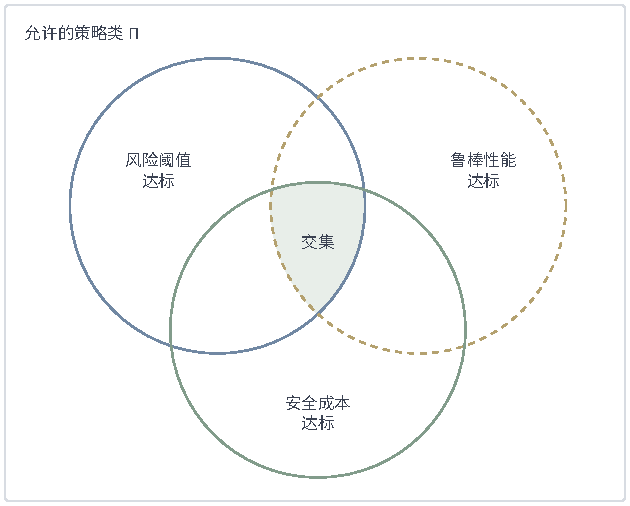
\includegraphics[width=106.652mm]{figures/10-reinforcement-learning/03-task-expansion-and-trustworthiness/tikz/rl-trustworthy-intersection.pdf}
  \caption{可行策略集合的概念示意，不是教学路线数值的几何嵌入。阴影为三种阈值共同允许的策略；在具体任务中，交集也可能为空。集合边界形状没有凸性含义。}
  \label{fig:rl-trustworthy-intersection}
\end{figure}

要识别保护器贡献，再固定同一候选，只切换保护是否启用。图~\ref{fig:rl-trustworthy-protected-path}~保留基准网格起终点和障碍，但采用无滑移的确定教学动力学，并将$(3,1)$规定为危险格。关闭保护，候选沿下方五步路径穿过危险格；启用保护，在$(2,1)$拒绝向右请求，转交已验证备份返回$(1,1)$，再沿上方到终点，共七步。该备份在这一确定模型中不进入障碍和危险格；恢复随机滑移后，须重新检查所有允许后继，原路径不能直接成为鲁棒安全证书。

\begin{figure}[htbp]
  \centering
  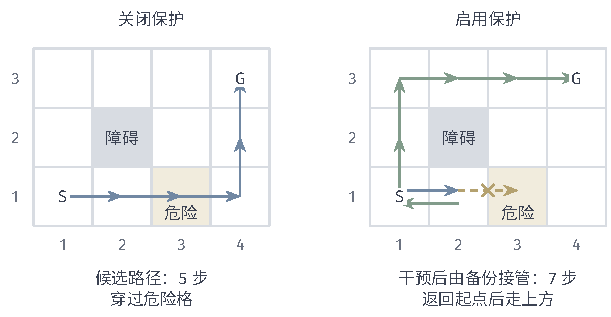
\includegraphics[width=103.470mm]{figures/10-reinforcement-learning/03-task-expansion-and-trustworthiness/tikz/rl-trustworthy-protected-path.pdf}
  \caption{同一候选启用或关闭保护的确定性路径示意，坐标、障碍和起终点沿用基准网格。虚线为被拒绝的请求，实线为实际路径；右图在干预后使用备份，不表示候选策略已自行学会绕行。}
  \label{fig:rl-trustworthy-protected-path}
\end{figure}

右图避免了一次危险格穿越，代价是两步额外行程和一次转入备份控制的切换。保持安全的是受保护系统，未保护候选仍请求经过危险格。图中一次拒绝也不等于全回合只替换一个动作，后续备份动作仍须由日志区分。保护改变了实际执行过程及其可见记录分布，学习器看到的安全轨迹可能来自外部修正；继续训练时须保留请求与实际动作，才能判断学到的是候选能力还是保护贡献。

这些比较同时呈现收益与代价。扩大不确定集合能增加覆盖范围，却可能降低可达到的回报；收紧尾部或安全阈值可能增加绕行与接管；加强保护能减少危险探索，却也会减少某些动作的观测，使其效果更难识别。因此方案结论需要同时声明行为标准、环境范围、执行机制与证据，单一平均分数不足以表达取舍。序贯决策的验证还须把其他已经明确的行为要求落实到实际策略、运行机制和评价记录，逐项规定可计算的指标、适用条件及证据。

% Outline: 8.7
\section{本章小结}
\label{sec:rl-trustworthy-summary}

导航例中，平均最快的路线未必尾部延误最小，尾部延误较小的路线未必耐受湿滑，耐受湿滑的路线又可能违反成本预算。风险准则比较随机后果，鲁棒要求覆盖允许环境，安全约束划定可行策略；三者可以组合，各自的评价目标、观测或环境模型要求及证明条件仍须分别保留。

\begin{table*}[htbp]
  \centering
  \begin{tabularx}{\linewidth}{@{}>{\raggedright\arraybackslash}p{22mm}XXX@{}}
    \toprule
    要求 & 决定性条件 & 方法 & 相应证据 \\
    \midrule
    控制累计尾部 & 损失、分位水平及事前承诺明确 & 静态CVaR采样更新、状态增广 & 尾部估计误差与留出轨迹 \\
    条件风险一致 & 条件映射及状态分量与递归目标匹配 & 嵌套风险Bellman更新 & 算子性质及条件风险估计 \\
    覆盖环境变化 & 扰动位置、扰动者可读字段与集合结构明确 & 鲁棒规划、受扰训练、状态估计 & 模型覆盖、内层误差与压力测试 \\
    平均成本达标 & 成本单位、初态、折扣及策略类明确 & 占用规划、原始--对偶与局部约束更新 & 最终策略的成本上界 \\
    事件概率达标 & 事件、时域、条件预算一致 & 事件采样、概率递推、预算分配 & 完整事件记录与有效概率上界 \\
    逐轨迹保持安全 & 误差范围有效、初态可行且保护输入存在 & 屏蔽、不变集、屏障与预测过滤 & 真实闭环符合证书全部前提 \\
    可靠地作出判断 & 交付对象、运行协议和取证程序固定 & 留出验证、联合置信与持续复核 & 界与阈值比较，并标明现有样本尚不足以判断达标 \\
    \bottomrule
  \end{tabularx}
  \caption{本章的要求、条件、方法与证据。算法的优化目标与交付时能够成立的保证是两件需要分别检查的事。}
  \label{tab:rl-trustworthy-summary}
\end{table*}

静态累计CVaR保留事前损失分布，嵌套风险逐层评价条件后果，状态增广与时间一致性要服务于对应目标。鲁棒备份须明确扰动作用于动力学、观测还是执行通道，并保存对手权限所需的状态；矩形性才使局部最坏选择组成合法模型。期望成本允许个别高成本轨迹，事件概率允许有限违约概率，硬要求则在声明范围内排除违约。乘子、概率预算和安全过滤据此维护不同性质。

表~\ref{tab:rl-trustworthy-summary}~对应每项要求的条件、方法与证据。方法的名称不足以判断可信性，还需确定它维护的性质、评价固定策略还是受保护系统、依赖哪些模型和记录采集前提，以及这些前提改变后哪些结论仍成立。



若日志支持不足或隐藏风险不可识别，需要回到第~\ref{chap:rl-information}~章的观测范围、日志字段与动作覆盖条件；若奖励没有表达真正意图，需要第~\ref{chap:rl-reward}~章的奖励分析。新任务识别与适应由第~\ref{chap:rl-transfer}~章讨论，其他参与者响应由第~\ref{chap:rl-multi-agent}~章提供模型。这些条件改变时，既要检查决策问题是否改变，也要复核原证据是否仍覆盖交付对象；求解结束本身并不构成可信性保证。


\clearpage
